\documentclass[twoside]{book}

% Packages required by doxygen
\usepackage{fixltx2e}
\usepackage{calc}
\usepackage{doxygen}
\usepackage[export]{adjustbox} % also loads graphicx
\usepackage{graphicx}
\usepackage[utf8]{inputenc}
\usepackage{makeidx}
\usepackage{multicol}
\usepackage{multirow}
\PassOptionsToPackage{warn}{textcomp}
\usepackage{textcomp}
\usepackage[nointegrals]{wasysym}
\usepackage[table]{xcolor}

% Font selection
\usepackage[T1]{fontenc}
\usepackage[scaled=.90]{helvet}
\usepackage{courier}
\usepackage{amssymb}
\usepackage{sectsty}
\renewcommand{\familydefault}{\sfdefault}
\allsectionsfont{%
  \fontseries{bc}\selectfont%
  \color{darkgray}%
}
\renewcommand{\DoxyLabelFont}{%
  \fontseries{bc}\selectfont%
  \color{darkgray}%
}
\newcommand{\+}{\discretionary{\mbox{\scriptsize$\hookleftarrow$}}{}{}}

% Page & text layout
\usepackage{geometry}
\geometry{%
  a4paper,%
  top=2.5cm,%
  bottom=2.5cm,%
  left=2.5cm,%
  right=2.5cm%
}
\tolerance=750
\hfuzz=15pt
\hbadness=750
\setlength{\emergencystretch}{15pt}
\setlength{\parindent}{0cm}
\setlength{\parskip}{3ex plus 2ex minus 2ex}
\makeatletter
\renewcommand{\paragraph}{%
  \@startsection{paragraph}{4}{0ex}{-1.0ex}{1.0ex}{%
    \normalfont\normalsize\bfseries\SS@parafont%
  }%
}
\renewcommand{\subparagraph}{%
  \@startsection{subparagraph}{5}{0ex}{-1.0ex}{1.0ex}{%
    \normalfont\normalsize\bfseries\SS@subparafont%
  }%
}
\makeatother

% Headers & footers
\usepackage{fancyhdr}
\pagestyle{fancyplain}
\fancyhead[LE]{\fancyplain{}{\bfseries\thepage}}
\fancyhead[CE]{\fancyplain{}{}}
\fancyhead[RE]{\fancyplain{}{\bfseries\leftmark}}
\fancyhead[LO]{\fancyplain{}{\bfseries\rightmark}}
\fancyhead[CO]{\fancyplain{}{}}
\fancyhead[RO]{\fancyplain{}{\bfseries\thepage}}
\fancyfoot[LE]{\fancyplain{}{}}
\fancyfoot[CE]{\fancyplain{}{}}
\fancyfoot[RE]{\fancyplain{}{\bfseries\scriptsize Generated by Doxygen }}
\fancyfoot[LO]{\fancyplain{}{\bfseries\scriptsize Generated by Doxygen }}
\fancyfoot[CO]{\fancyplain{}{}}
\fancyfoot[RO]{\fancyplain{}{}}
\renewcommand{\footrulewidth}{0.4pt}
\renewcommand{\chaptermark}[1]{%
  \markboth{#1}{}%
}
\renewcommand{\sectionmark}[1]{%
  \markright{\thesection\ #1}%
}

% Indices & bibliography
\usepackage{natbib}
\usepackage[titles]{tocloft}
\setcounter{tocdepth}{3}
\setcounter{secnumdepth}{5}
\makeindex

% Hyperlinks (required, but should be loaded last)
\usepackage{ifpdf}
\ifpdf
  \usepackage[pdftex,pagebackref=true]{hyperref}
\else
  \usepackage[ps2pdf,pagebackref=true]{hyperref}
\fi
\hypersetup{%
  colorlinks=true,%
  linkcolor=blue,%
  citecolor=blue,%
  unicode%
}

% Custom commands
\newcommand{\clearemptydoublepage}{%
  \newpage{\pagestyle{empty}\cleardoublepage}%
}

\usepackage{caption}
\captionsetup{labelsep=space,justification=centering,font={bf},singlelinecheck=off,skip=4pt,position=top}

%===== C O N T E N T S =====

\begin{document}

% Titlepage & ToC
\hypersetup{pageanchor=false,
             bookmarksnumbered=true,
             pdfencoding=unicode
            }
\pagenumbering{roman}
\begin{titlepage}
\vspace*{7cm}
\begin{center}%
{\Large Ricci\+Flow\+Extremal\+Length }\\
\vspace*{1cm}
{\large Generated by Doxygen 1.8.11}\\
\end{center}
\end{titlepage}
\clearemptydoublepage
\tableofcontents
\clearemptydoublepage
\pagenumbering{arabic}
\hypersetup{pageanchor=true}

%--- Begin generated contents ---
\chapter{Namespace Index}
\section{Namespace List}
Here is a list of all namespaces with brief descriptions\+:\begin{DoxyCompactList}
\item\contentsline{section}{\hyperlink{namespace_mesh_lib}{Mesh\+Lib} }{\pageref{namespace_mesh_lib}}{}
\item\contentsline{section}{\hyperlink{namespacestrutil}{strutil} }{\pageref{namespacestrutil}}{}
\end{DoxyCompactList}

\chapter{Hierarchical Index}
\section{Class Hierarchy}
This inheritance list is sorted roughly, but not completely, alphabetically\+:\begin{DoxyCompactList}
\item \contentsline{section}{Mesh\+Lib\+:\+:C\+Base\+Embed$<$ C\+Vertex, C\+Edge, C\+Face, C\+Half\+Edge $>$}{\pageref{class_mesh_lib_1_1_c_base_embed}}{}
\begin{DoxyCompactList}
\item \contentsline{section}{Mesh\+Lib\+:\+:C\+Euclidean\+Embed$<$ C\+Vertex, C\+Edge, C\+Face, C\+Half\+Edge $>$}{\pageref{class_mesh_lib_1_1_c_euclidean_embed}}{}
\end{DoxyCompactList}
\item \contentsline{section}{Mesh\+Lib\+:\+:C\+Base\+Mesh$<$ C\+Vertex, C\+Edge, C\+Face, C\+Half\+Edge $>$}{\pageref{class_mesh_lib_1_1_c_base_mesh}}{}
\item \contentsline{section}{Mesh\+Lib\+:\+:C\+Base\+Mesh$<$ Mesh\+Lib\+:\+:C\+Vertex, Mesh\+Lib\+:\+:C\+Edge, Mesh\+Lib\+:\+:C\+Face, Mesh\+Lib\+:\+:C\+Half\+Edge $>$}{\pageref{class_mesh_lib_1_1_c_base_mesh}}{}
\item \contentsline{section}{Mesh\+Lib\+:\+:C\+Base\+Mesh$<$ Mesh\+Lib\+:\+:V, Mesh\+Lib\+:\+:E, Mesh\+Lib\+:\+:F, Mesh\+Lib\+:\+:H $>$}{\pageref{class_mesh_lib_1_1_c_base_mesh}}{}
\item \contentsline{section}{Mesh\+Lib\+:\+:C\+Base\+Mesh$<$ V, E, F, H $>$}{\pageref{class_mesh_lib_1_1_c_base_mesh}}{}
\begin{DoxyCompactList}
\item \contentsline{section}{Mesh\+Lib\+:\+:C\+Dynamic\+Mesh$<$ V, E, F, H $>$}{\pageref{class_mesh_lib_1_1_c_dynamic_mesh}}{}
\end{DoxyCompactList}
\item \contentsline{section}{Mesh\+Lib\+:\+:C\+Base\+Ricci\+Flow$<$ V, E, F, H $>$}{\pageref{class_mesh_lib_1_1_c_base_ricci_flow}}{}
\begin{DoxyCompactList}
\item \contentsline{section}{Mesh\+Lib\+:\+:C\+Tangential\+Ricci\+Flow$<$ V, E, F, H $>$}{\pageref{class_mesh_lib_1_1_c_tangential_ricci_flow}}{}
\begin{DoxyCompactList}
\item \contentsline{section}{Mesh\+Lib\+:\+:C\+Tangential\+Ricci\+Flow\+Extremal\+Length$<$ V, E, F, H $>$}{\pageref{class_mesh_lib_1_1_c_tangential_ricci_flow_extremal_length}}{}
\end{DoxyCompactList}
\end{DoxyCompactList}
\item \contentsline{section}{Mesh\+Lib\+:\+:C\+Boundary$<$ C\+Vertex, C\+Edge, C\+Face, C\+Half\+Edge $>$}{\pageref{class_mesh_lib_1_1_c_boundary}}{}
\item \contentsline{section}{Mesh\+Lib\+:\+:C\+Boundary$<$ V, E, F, H $>$}{\pageref{class_mesh_lib_1_1_c_boundary}}{}
\item \contentsline{section}{Mesh\+Lib\+:\+:C\+Circle}{\pageref{class_mesh_lib_1_1_c_circle}}{}
\item \contentsline{section}{Mesh\+Lib\+:\+:C\+Edge}{\pageref{class_mesh_lib_1_1_c_edge}}{}
\item \contentsline{section}{Mesh\+Lib\+:\+:C\+Face}{\pageref{class_mesh_lib_1_1_c_face}}{}
\item \contentsline{section}{Mesh\+Lib\+:\+:C\+Half\+Edge}{\pageref{class_mesh_lib_1_1_c_half_edge}}{}
\item \contentsline{section}{Mesh\+Lib\+:\+:C\+Loop$<$ C\+Vertex, C\+Edge, C\+Face, C\+Half\+Edge $>$}{\pageref{class_mesh_lib_1_1_c_loop}}{}
\item \contentsline{section}{Mesh\+Lib\+:\+:C\+Parser}{\pageref{class_mesh_lib_1_1_c_parser}}{}
\item \contentsline{section}{Mesh\+Lib\+:\+:C\+Point}{\pageref{class_mesh_lib_1_1_c_point}}{}
\item \contentsline{section}{Mesh\+Lib\+:\+:C\+Point2}{\pageref{class_mesh_lib_1_1_c_point2}}{}
\item \contentsline{section}{Mesh\+Lib\+:\+:C\+Structure$<$ Mesh, V, E, F, H $>$}{\pageref{class_mesh_lib_1_1_c_structure}}{}
\item \contentsline{section}{Mesh\+Lib\+:\+:C\+Token}{\pageref{class_mesh_lib_1_1_c_token}}{}
\item \contentsline{section}{Mesh\+Lib\+:\+:C\+Vertex}{\pageref{class_mesh_lib_1_1_c_vertex}}{}
\begin{DoxyCompactList}
\item \contentsline{section}{Mesh\+Lib\+:\+:C\+Ricci\+Flow\+Vertex}{\pageref{class_mesh_lib_1_1_c_ricci_flow_vertex}}{}
\end{DoxyCompactList}
\item \contentsline{section}{Mesh\+Lib\+:\+:Face\+Edge\+Iterator$<$ C\+Vertex, C\+Edge, C\+Face, C\+Half\+Edge $>$}{\pageref{class_mesh_lib_1_1_face_edge_iterator}}{}
\item \contentsline{section}{Mesh\+Lib\+:\+:Face\+Halfedge\+Iterator$<$ C\+Vertex, C\+Edge, C\+Face, C\+Half\+Edge $>$}{\pageref{class_mesh_lib_1_1_face_halfedge_iterator}}{}
\item \contentsline{section}{Mesh\+Lib\+:\+:Face\+Vertex\+Iterator$<$ C\+Vertex, C\+Edge, C\+Face, C\+Half\+Edge $>$}{\pageref{class_mesh_lib_1_1_face_vertex_iterator}}{}
\item \contentsline{section}{Mesh\+Lib\+:\+:Mesh\+Edge\+Iterator$<$ C\+Vertex, C\+Edge, C\+Face, C\+Half\+Edge $>$}{\pageref{class_mesh_lib_1_1_mesh_edge_iterator}}{}
\item \contentsline{section}{Mesh\+Lib\+:\+:Mesh\+Face\+Iterator$<$ C\+Vertex, C\+Edge, C\+Face, C\+Half\+Edge $>$}{\pageref{class_mesh_lib_1_1_mesh_face_iterator}}{}
\item \contentsline{section}{Mesh\+Lib\+:\+:Mesh\+Half\+Edge\+Iterator$<$ C\+Vertex, C\+Edge, C\+Face, C\+Half\+Edge $>$}{\pageref{class_mesh_lib_1_1_mesh_half_edge_iterator}}{}
\item \contentsline{section}{Mesh\+Lib\+:\+:Mesh\+Vertex\+Iterator$<$ C\+Vertex, C\+Edge, C\+Face, C\+Half\+Edge $>$}{\pageref{class_mesh_lib_1_1_mesh_vertex_iterator}}{}
\item \contentsline{section}{strutil\+:\+:Tokenizer}{\pageref{classstrutil_1_1_tokenizer}}{}
\item \contentsline{section}{Mesh\+Lib\+:\+:Vertex\+Edge\+Iterator$<$ C\+Vertex, C\+Edge, C\+Face, C\+Half\+Edge $>$}{\pageref{class_mesh_lib_1_1_vertex_edge_iterator}}{}
\item \contentsline{section}{Mesh\+Lib\+:\+:Vertex\+Face\+Iterator$<$ C\+Vertex, C\+Edge, C\+Face, C\+Half\+Edge $>$}{\pageref{class_mesh_lib_1_1_vertex_face_iterator}}{}
\item \contentsline{section}{Mesh\+Lib\+:\+:Vertex\+In\+Halfedge\+Iterator$<$ C\+Vertex, C\+Edge, C\+Face, C\+Half\+Edge $>$}{\pageref{class_mesh_lib_1_1_vertex_in_halfedge_iterator}}{}
\item \contentsline{section}{Mesh\+Lib\+:\+:Vertex\+Out\+Halfedge\+Iterator$<$ C\+Vertex, C\+Edge, C\+Face, C\+Half\+Edge $>$}{\pageref{class_mesh_lib_1_1_vertex_out_halfedge_iterator}}{}
\item \contentsline{section}{Mesh\+Lib\+:\+:Vertex\+Vertex\+Iterator$<$ C\+Vertex, C\+Edge, C\+Face, C\+Half\+Edge $>$}{\pageref{class_mesh_lib_1_1_vertex_vertex_iterator}}{}
\end{DoxyCompactList}

\chapter{Class Index}
\section{Class List}
Here are the classes, structs, unions and interfaces with brief descriptions\+:\begin{DoxyCompactList}
\item\contentsline{section}{\hyperlink{class_mesh_lib_1_1_c_base_embed}{Mesh\+Lib\+::\+C\+Base\+Embed$<$ C\+Vertex, C\+Edge, C\+Face, C\+Half\+Edge $>$} \\*\hyperlink{class_mesh_lib_1_1_c_base_embed}{C\+Base\+Embed} class }{\pageref{class_mesh_lib_1_1_c_base_embed}}{}
\item\contentsline{section}{\hyperlink{class_mesh_lib_1_1_c_base_mesh}{Mesh\+Lib\+::\+C\+Base\+Mesh$<$ C\+Vertex, C\+Edge, C\+Face, C\+Half\+Edge $>$} \\*\hyperlink{class_mesh_lib_1_1_c_base_mesh}{C\+Base\+Mesh}, base class for all types of mesh classes }{\pageref{class_mesh_lib_1_1_c_base_mesh}}{}
\item\contentsline{section}{\hyperlink{class_mesh_lib_1_1_c_base_ricci_flow}{Mesh\+Lib\+::\+C\+Base\+Ricci\+Flow$<$ V, E, F, H $>$} \\*Base\+Class \hyperlink{class_mesh_lib_1_1_c_base_ricci_flow}{C\+Base\+Ricci\+Flow} }{\pageref{class_mesh_lib_1_1_c_base_ricci_flow}}{}
\item\contentsline{section}{\hyperlink{class_mesh_lib_1_1_c_boundary}{Mesh\+Lib\+::\+C\+Boundary$<$ C\+Vertex, C\+Edge, C\+Face, C\+Half\+Edge $>$} \\*\hyperlink{class_mesh_lib_1_1_c_boundary}{C\+Boundary} Boundary class }{\pageref{class_mesh_lib_1_1_c_boundary}}{}
\item\contentsline{section}{\hyperlink{class_mesh_lib_1_1_c_circle}{Mesh\+Lib\+::\+C\+Circle} \\*\hyperlink{class_mesh_lib_1_1_c_circle}{C\+Circle} class, circle on the plane }{\pageref{class_mesh_lib_1_1_c_circle}}{}
\item\contentsline{section}{\hyperlink{class_mesh_lib_1_1_c_dynamic_mesh}{Mesh\+Lib\+::\+C\+Dynamic\+Mesh$<$ V, E, F, H $>$} \\*\hyperlink{class_mesh_lib_1_1_c_dynamic_mesh}{C\+Dynamic\+Mesh} class \+: Dynamic mesh }{\pageref{class_mesh_lib_1_1_c_dynamic_mesh}}{}
\item\contentsline{section}{\hyperlink{class_mesh_lib_1_1_c_edge}{Mesh\+Lib\+::\+C\+Edge} \\*\hyperlink{class_mesh_lib_1_1_c_edge}{C\+Edge} class, which is the base class of all kinds of edge classes }{\pageref{class_mesh_lib_1_1_c_edge}}{}
\item\contentsline{section}{\hyperlink{class_mesh_lib_1_1_c_euclidean_embed}{Mesh\+Lib\+::\+C\+Euclidean\+Embed$<$ C\+Vertex, C\+Edge, C\+Face, C\+Half\+Edge $>$} \\*C\+Embed class }{\pageref{class_mesh_lib_1_1_c_euclidean_embed}}{}
\item\contentsline{section}{\hyperlink{class_mesh_lib_1_1_c_face}{Mesh\+Lib\+::\+C\+Face} \\*\hyperlink{class_mesh_lib_1_1_c_face}{C\+Face} base class of all kinds of face classes }{\pageref{class_mesh_lib_1_1_c_face}}{}
\item\contentsline{section}{\hyperlink{class_mesh_lib_1_1_c_half_edge}{Mesh\+Lib\+::\+C\+Half\+Edge} \\*\hyperlink{class_mesh_lib_1_1_c_half_edge}{C\+Half\+Edge} Base class of all kinds of halfedges }{\pageref{class_mesh_lib_1_1_c_half_edge}}{}
\item\contentsline{section}{\hyperlink{class_mesh_lib_1_1_c_loop}{Mesh\+Lib\+::\+C\+Loop$<$ C\+Vertex, C\+Edge, C\+Face, C\+Half\+Edge $>$} \\*\hyperlink{class_mesh_lib_1_1_c_loop}{C\+Loop} Boundary loop class }{\pageref{class_mesh_lib_1_1_c_loop}}{}
\item\contentsline{section}{\hyperlink{class_mesh_lib_1_1_c_parser}{Mesh\+Lib\+::\+C\+Parser} \\*\hyperlink{class_mesh_lib_1_1_c_parser}{C\+Parser} class }{\pageref{class_mesh_lib_1_1_c_parser}}{}
\item\contentsline{section}{\hyperlink{class_mesh_lib_1_1_c_point}{Mesh\+Lib\+::\+C\+Point} \\*\hyperlink{class_mesh_lib_1_1_c_point}{C\+Point} class, three dimensional point }{\pageref{class_mesh_lib_1_1_c_point}}{}
\item\contentsline{section}{\hyperlink{class_mesh_lib_1_1_c_point2}{Mesh\+Lib\+::\+C\+Point2} \\*\hyperlink{class_mesh_lib_1_1_c_point2}{C\+Point2} class, two dimensional point }{\pageref{class_mesh_lib_1_1_c_point2}}{}
\item\contentsline{section}{\hyperlink{class_mesh_lib_1_1_c_ricci_flow_vertex}{Mesh\+Lib\+::\+C\+Ricci\+Flow\+Vertex} \\*\hyperlink{class_mesh_lib_1_1_c_ricci_flow_vertex}{C\+Ricci\+Flow\+Vertex} class }{\pageref{class_mesh_lib_1_1_c_ricci_flow_vertex}}{}
\item\contentsline{section}{\hyperlink{class_mesh_lib_1_1_c_structure}{Mesh\+Lib\+::\+C\+Structure$<$ Mesh, V, E, F, H $>$} \\*Conversion class }{\pageref{class_mesh_lib_1_1_c_structure}}{}
\item\contentsline{section}{\hyperlink{class_mesh_lib_1_1_c_tangential_ricci_flow}{Mesh\+Lib\+::\+C\+Tangential\+Ricci\+Flow$<$ V, E, F, H $>$} \\*Class \hyperlink{class_mesh_lib_1_1_c_tangential_ricci_flow}{C\+Tangential\+Ricci\+Flow} }{\pageref{class_mesh_lib_1_1_c_tangential_ricci_flow}}{}
\item\contentsline{section}{\hyperlink{class_mesh_lib_1_1_c_tangential_ricci_flow_extremal_length}{Mesh\+Lib\+::\+C\+Tangential\+Ricci\+Flow\+Extremal\+Length$<$ V, E, F, H $>$} \\*C\+Inversive\+Distance\+Ricci\+Flow\+Extremal\+Length class }{\pageref{class_mesh_lib_1_1_c_tangential_ricci_flow_extremal_length}}{}
\item\contentsline{section}{\hyperlink{class_mesh_lib_1_1_c_token}{Mesh\+Lib\+::\+C\+Token} \\*\hyperlink{class_mesh_lib_1_1_c_token}{C\+Token} class, key=(value), e.\+g. uv=(x y) }{\pageref{class_mesh_lib_1_1_c_token}}{}
\item\contentsline{section}{\hyperlink{class_mesh_lib_1_1_c_vertex}{Mesh\+Lib\+::\+C\+Vertex} \\*\hyperlink{class_mesh_lib_1_1_c_vertex}{C\+Vertex} class, which is the base class of all kinds of vertex classes }{\pageref{class_mesh_lib_1_1_c_vertex}}{}
\item\contentsline{section}{\hyperlink{class_mesh_lib_1_1_face_edge_iterator}{Mesh\+Lib\+::\+Face\+Edge\+Iterator$<$ C\+Vertex, C\+Edge, C\+Face, C\+Half\+Edge $>$} \\*\hyperlink{class_mesh_lib_1_1_face_edge_iterator}{Face\+Edge\+Iterator}, transverse all the edges of a face C\+C\+Wly }{\pageref{class_mesh_lib_1_1_face_edge_iterator}}{}
\item\contentsline{section}{\hyperlink{class_mesh_lib_1_1_face_halfedge_iterator}{Mesh\+Lib\+::\+Face\+Halfedge\+Iterator$<$ C\+Vertex, C\+Edge, C\+Face, C\+Half\+Edge $>$} \\*\hyperlink{class_mesh_lib_1_1_face_halfedge_iterator}{Face\+Halfedge\+Iterator}, transverse all the halfedges of a face C\+C\+Wly }{\pageref{class_mesh_lib_1_1_face_halfedge_iterator}}{}
\item\contentsline{section}{\hyperlink{class_mesh_lib_1_1_face_vertex_iterator}{Mesh\+Lib\+::\+Face\+Vertex\+Iterator$<$ C\+Vertex, C\+Edge, C\+Face, C\+Half\+Edge $>$} \\*\hyperlink{class_mesh_lib_1_1_face_vertex_iterator}{Face\+Vertex\+Iterator}, transverse all the vertices of a face C\+C\+Wly }{\pageref{class_mesh_lib_1_1_face_vertex_iterator}}{}
\item\contentsline{section}{\hyperlink{class_mesh_lib_1_1_mesh_edge_iterator}{Mesh\+Lib\+::\+Mesh\+Edge\+Iterator$<$ C\+Vertex, C\+Edge, C\+Face, C\+Half\+Edge $>$} \\*\hyperlink{class_mesh_lib_1_1_mesh_edge_iterator}{Mesh\+Edge\+Iterator}, transverse all the edges in the mesh }{\pageref{class_mesh_lib_1_1_mesh_edge_iterator}}{}
\item\contentsline{section}{\hyperlink{class_mesh_lib_1_1_mesh_face_iterator}{Mesh\+Lib\+::\+Mesh\+Face\+Iterator$<$ C\+Vertex, C\+Edge, C\+Face, C\+Half\+Edge $>$} \\*\hyperlink{class_mesh_lib_1_1_mesh_face_iterator}{Mesh\+Face\+Iterator}, transverse all the faces in the mesh }{\pageref{class_mesh_lib_1_1_mesh_face_iterator}}{}
\item\contentsline{section}{\hyperlink{class_mesh_lib_1_1_mesh_half_edge_iterator}{Mesh\+Lib\+::\+Mesh\+Half\+Edge\+Iterator$<$ C\+Vertex, C\+Edge, C\+Face, C\+Half\+Edge $>$} \\*\hyperlink{class_mesh_lib_1_1_mesh_half_edge_iterator}{Mesh\+Half\+Edge\+Iterator}, transverse all the halfedges in the mesh }{\pageref{class_mesh_lib_1_1_mesh_half_edge_iterator}}{}
\item\contentsline{section}{\hyperlink{class_mesh_lib_1_1_mesh_vertex_iterator}{Mesh\+Lib\+::\+Mesh\+Vertex\+Iterator$<$ C\+Vertex, C\+Edge, C\+Face, C\+Half\+Edge $>$} \\*\hyperlink{class_mesh_lib_1_1_mesh_vertex_iterator}{Mesh\+Vertex\+Iterator}, transverse all the vertices in the mesh }{\pageref{class_mesh_lib_1_1_mesh_vertex_iterator}}{}
\item\contentsline{section}{\hyperlink{classstrutil_1_1_tokenizer}{strutil\+::\+Tokenizer} \\*String \hyperlink{classstrutil_1_1_tokenizer}{Tokenizer} }{\pageref{classstrutil_1_1_tokenizer}}{}
\item\contentsline{section}{\hyperlink{class_mesh_lib_1_1_vertex_edge_iterator}{Mesh\+Lib\+::\+Vertex\+Edge\+Iterator$<$ C\+Vertex, C\+Edge, C\+Face, C\+Half\+Edge $>$} \\*\hyperlink{class_mesh_lib_1_1_vertex_edge_iterator}{Vertex\+Edge\+Iterator}, transverse all the neighboring edges of a vertex ccwly }{\pageref{class_mesh_lib_1_1_vertex_edge_iterator}}{}
\item\contentsline{section}{\hyperlink{class_mesh_lib_1_1_vertex_face_iterator}{Mesh\+Lib\+::\+Vertex\+Face\+Iterator$<$ C\+Vertex, C\+Edge, C\+Face, C\+Half\+Edge $>$} \\*\hyperlink{class_mesh_lib_1_1_vertex_face_iterator}{Vertex\+Face\+Iterator}, transverse all the neighboring faces of a vertex ccwly }{\pageref{class_mesh_lib_1_1_vertex_face_iterator}}{}
\item\contentsline{section}{\hyperlink{class_mesh_lib_1_1_vertex_in_halfedge_iterator}{Mesh\+Lib\+::\+Vertex\+In\+Halfedge\+Iterator$<$ C\+Vertex, C\+Edge, C\+Face, C\+Half\+Edge $>$} \\*\hyperlink{class_mesh_lib_1_1_vertex_in_halfedge_iterator}{Vertex\+In\+Halfedge\+Iterator}, transverse all the incoming halfedges of a vertex ccwly }{\pageref{class_mesh_lib_1_1_vertex_in_halfedge_iterator}}{}
\item\contentsline{section}{\hyperlink{class_mesh_lib_1_1_vertex_out_halfedge_iterator}{Mesh\+Lib\+::\+Vertex\+Out\+Halfedge\+Iterator$<$ C\+Vertex, C\+Edge, C\+Face, C\+Half\+Edge $>$} \\*\hyperlink{class_mesh_lib_1_1_vertex_out_halfedge_iterator}{Vertex\+Out\+Halfedge\+Iterator}, transverse all the outgoing halfedges of a vertex ccwly }{\pageref{class_mesh_lib_1_1_vertex_out_halfedge_iterator}}{}
\item\contentsline{section}{\hyperlink{class_mesh_lib_1_1_vertex_vertex_iterator}{Mesh\+Lib\+::\+Vertex\+Vertex\+Iterator$<$ C\+Vertex, C\+Edge, C\+Face, C\+Half\+Edge $>$} \\*\hyperlink{class_mesh_lib_1_1_vertex_vertex_iterator}{Vertex\+Vertex\+Iterator}, transverse all the neighboring vertices of a vertex ccwly }{\pageref{class_mesh_lib_1_1_vertex_vertex_iterator}}{}
\end{DoxyCompactList}

\chapter{File Index}
\section{File List}
Here is a list of all files with brief descriptions\+:\begin{DoxyCompactList}
\item\contentsline{section}{Mesh\+Lib/algorithm/\+Riemannian/\+Ricci\+Flow/\hyperlink{_base_embed_8h}{Base\+Embed.\+h} \\*Isometrically embed a mesh with canonical metric onto the canonical domain }{\pageref{_base_embed_8h}}{}
\item\contentsline{section}{Mesh\+Lib/algorithm/\+Riemannian/\+Ricci\+Flow/\hyperlink{_base_ricci_flow_8h}{Base\+Ricci\+Flow.\+h} \\*Base class for Ricci flow algorithm }{\pageref{_base_ricci_flow_8h}}{}
\item\contentsline{section}{Mesh\+Lib/algorithm/\+Riemannian/\+Ricci\+Flow/\hyperlink{_euclidean_embed_8h}{Euclidean\+Embed.\+h} \\*Isometrically embed a mesh with flat metric onto the plane }{\pageref{_euclidean_embed_8h}}{}
\item\contentsline{section}{Mesh\+Lib/algorithm/\+Riemannian/\+Ricci\+Flow/\hyperlink{_ricci_flow_mesh_8h}{Ricci\+Flow\+Mesh.\+h} \\*Mesh for Ricci Flow }{\pageref{_ricci_flow_mesh_8h}}{}
\item\contentsline{section}{Mesh\+Lib/algorithm/\+Riemannian/\+Ricci\+Flow/\hyperlink{_tangential_ricci_extremal_length_8h}{Tangential\+Ricci\+Extremal\+Length.\+h} \\*Euclidean Tangential Ricci flow for Extremal Length }{\pageref{_tangential_ricci_extremal_length_8h}}{}
\item\contentsline{section}{Mesh\+Lib/algorithm/\+Riemannian/\+Ricci\+Flow/\hyperlink{_tangential_ricci_flow_8h}{Tangential\+Ricci\+Flow.\+h} \\*General Euclidean Ricci flow algorithm }{\pageref{_tangential_ricci_flow_8h}}{}
\item\contentsline{section}{Mesh\+Lib/algorithm/\+Structure/\hyperlink{_structure_8h}{Structure.\+h} \\*Algorithms for converting one structure to another }{\pageref{_structure_8h}}{}
\item\contentsline{section}{Mesh\+Lib/core/\+Geometry/\hyperlink{_circle_8h}{Circle.\+h} \\*Planar circle }{\pageref{_circle_8h}}{}
\item\contentsline{section}{Mesh\+Lib/core/\+Geometry/\hyperlink{_point_8h}{Point.\+h} \\*Three dimensional point class }{\pageref{_point_8h}}{}
\item\contentsline{section}{Mesh\+Lib/core/\+Geometry/\hyperlink{_point2_8h}{Point2.\+h} \\*Two dimensional point class }{\pageref{_point2_8h}}{}
\item\contentsline{section}{Mesh\+Lib/core/\+Mesh/\hyperlink{_base_mesh_8h}{Base\+Mesh.\+h} \\*Base Mesh Class for all types of Mesh Classes }{\pageref{_base_mesh_8h}}{}
\item\contentsline{section}{Mesh\+Lib/core/\+Mesh/\hyperlink{boundary_8h}{boundary.\+h} }{\pageref{boundary_8h}}{}
\item\contentsline{section}{Mesh\+Lib/core/\+Mesh/\hyperlink{_dynamic_mesh_8h}{Dynamic\+Mesh.\+h} \\*Dynamic Mesh Class for edge swap, face split, edge split }{\pageref{_dynamic_mesh_8h}}{}
\item\contentsline{section}{Mesh\+Lib/core/\+Mesh/\hyperlink{_edge_8h}{Edge.\+h} \\*Base class of edge }{\pageref{_edge_8h}}{}
\item\contentsline{section}{Mesh\+Lib/core/\+Mesh/\hyperlink{_face_8h}{Face.\+h} \\*Base class of face }{\pageref{_face_8h}}{}
\item\contentsline{section}{Mesh\+Lib/core/\+Mesh/\hyperlink{_half_edge_8h}{Half\+Edge.\+h} \\*Base class of Half\+Edge }{\pageref{_half_edge_8h}}{}
\item\contentsline{section}{Mesh\+Lib/core/\+Mesh/\hyperlink{iterators_8h}{iterators.\+h} }{\pageref{iterators_8h}}{}
\item\contentsline{section}{Mesh\+Lib/core/\+Mesh/\hyperlink{_vertex_8h}{Vertex.\+h} \\*Base class of vertex }{\pageref{_vertex_8h}}{}
\item\contentsline{section}{Mesh\+Lib/core/\+Parser/\hyperlink{parser_8h}{parser.\+h} \\*Parse the trait strings of vertex, edge, halfedge , face etc }{\pageref{parser_8h}}{}
\item\contentsline{section}{Mesh\+Lib/core/\+Parser/\hyperlink{strutil_8h}{strutil.\+h} \\*Std\+::string utilities }{\pageref{strutil_8h}}{}
\item\contentsline{section}{Mesh\+Lib/core/\+Parser/\hyperlink{traits__io_8h}{traits\+\_\+io.\+h} }{\pageref{traits__io_8h}}{}
\end{DoxyCompactList}

\chapter{Namespace Documentation}
\hypertarget{namespace_mesh_lib}{}\section{Mesh\+Lib Namespace Reference}
\label{namespace_mesh_lib}\index{Mesh\+Lib@{Mesh\+Lib}}
\subsection*{Classes}
\begin{DoxyCompactItemize}
\item 
class \hyperlink{class_mesh_lib_1_1_c_base_embed}{C\+Base\+Embed}
\begin{DoxyCompactList}\small\item\em \hyperlink{class_mesh_lib_1_1_c_base_embed}{C\+Base\+Embed} class. \end{DoxyCompactList}\item 
class \hyperlink{class_mesh_lib_1_1_c_base_mesh}{C\+Base\+Mesh}
\begin{DoxyCompactList}\small\item\em \hyperlink{class_mesh_lib_1_1_c_base_mesh}{C\+Base\+Mesh}, base class for all types of mesh classes. \end{DoxyCompactList}\item 
class \hyperlink{class_mesh_lib_1_1_c_base_ricci_flow}{C\+Base\+Ricci\+Flow}
\begin{DoxyCompactList}\small\item\em Base\+Class \hyperlink{class_mesh_lib_1_1_c_base_ricci_flow}{C\+Base\+Ricci\+Flow}. \end{DoxyCompactList}\item 
class \hyperlink{class_mesh_lib_1_1_c_boundary}{C\+Boundary}
\begin{DoxyCompactList}\small\item\em \hyperlink{class_mesh_lib_1_1_c_boundary}{C\+Boundary} Boundary class. \end{DoxyCompactList}\item 
class \hyperlink{class_mesh_lib_1_1_c_circle}{C\+Circle}
\begin{DoxyCompactList}\small\item\em \hyperlink{class_mesh_lib_1_1_c_circle}{C\+Circle} class, circle on the plane. \end{DoxyCompactList}\item 
class \hyperlink{class_mesh_lib_1_1_c_dynamic_mesh}{C\+Dynamic\+Mesh}
\begin{DoxyCompactList}\small\item\em \hyperlink{class_mesh_lib_1_1_c_dynamic_mesh}{C\+Dynamic\+Mesh} class \+: Dynamic mesh. \end{DoxyCompactList}\item 
class \hyperlink{class_mesh_lib_1_1_c_edge}{C\+Edge}
\begin{DoxyCompactList}\small\item\em \hyperlink{class_mesh_lib_1_1_c_edge}{C\+Edge} class, which is the base class of all kinds of edge classes. \end{DoxyCompactList}\item 
class \hyperlink{class_mesh_lib_1_1_c_euclidean_embed}{C\+Euclidean\+Embed}
\begin{DoxyCompactList}\small\item\em C\+Embed class. \end{DoxyCompactList}\item 
class \hyperlink{class_mesh_lib_1_1_c_face}{C\+Face}
\begin{DoxyCompactList}\small\item\em \hyperlink{class_mesh_lib_1_1_c_face}{C\+Face} base class of all kinds of face classes. \end{DoxyCompactList}\item 
class \hyperlink{class_mesh_lib_1_1_c_half_edge}{C\+Half\+Edge}
\begin{DoxyCompactList}\small\item\em \hyperlink{class_mesh_lib_1_1_c_half_edge}{C\+Half\+Edge} Base class of all kinds of halfedges. \end{DoxyCompactList}\item 
class \hyperlink{class_mesh_lib_1_1_c_loop}{C\+Loop}
\begin{DoxyCompactList}\small\item\em \hyperlink{class_mesh_lib_1_1_c_loop}{C\+Loop} Boundary loop class. \end{DoxyCompactList}\item 
class \hyperlink{class_mesh_lib_1_1_c_parser}{C\+Parser}
\begin{DoxyCompactList}\small\item\em \hyperlink{class_mesh_lib_1_1_c_parser}{C\+Parser} class. \end{DoxyCompactList}\item 
class \hyperlink{class_mesh_lib_1_1_c_point}{C\+Point}
\begin{DoxyCompactList}\small\item\em \hyperlink{class_mesh_lib_1_1_c_point}{C\+Point} class, three dimensional point. \end{DoxyCompactList}\item 
class \hyperlink{class_mesh_lib_1_1_c_point2}{C\+Point2}
\begin{DoxyCompactList}\small\item\em \hyperlink{class_mesh_lib_1_1_c_point2}{C\+Point2} class, two dimensional point. \end{DoxyCompactList}\item 
class \hyperlink{class_mesh_lib_1_1_c_ricci_flow_vertex}{C\+Ricci\+Flow\+Vertex}
\begin{DoxyCompactList}\small\item\em \hyperlink{class_mesh_lib_1_1_c_ricci_flow_vertex}{C\+Ricci\+Flow\+Vertex} class. \end{DoxyCompactList}\item 
class \hyperlink{class_mesh_lib_1_1_c_structure}{C\+Structure}
\begin{DoxyCompactList}\small\item\em Conversion class. \end{DoxyCompactList}\item 
class \hyperlink{class_mesh_lib_1_1_c_tangential_ricci_flow}{C\+Tangential\+Ricci\+Flow}
\begin{DoxyCompactList}\small\item\em Class \hyperlink{class_mesh_lib_1_1_c_tangential_ricci_flow}{C\+Tangential\+Ricci\+Flow}. \end{DoxyCompactList}\item 
class \hyperlink{class_mesh_lib_1_1_c_tangential_ricci_flow_extremal_length}{C\+Tangential\+Ricci\+Flow\+Extremal\+Length}
\begin{DoxyCompactList}\small\item\em C\+Inversive\+Distance\+Ricci\+Flow\+Extremal\+Length class. \end{DoxyCompactList}\item 
class \hyperlink{class_mesh_lib_1_1_c_token}{C\+Token}
\begin{DoxyCompactList}\small\item\em \hyperlink{class_mesh_lib_1_1_c_token}{C\+Token} class, key=(value), e.\+g. uv=(x y) \end{DoxyCompactList}\item 
class \hyperlink{class_mesh_lib_1_1_c_vertex}{C\+Vertex}
\begin{DoxyCompactList}\small\item\em \hyperlink{class_mesh_lib_1_1_c_vertex}{C\+Vertex} class, which is the base class of all kinds of vertex classes. \end{DoxyCompactList}\item 
class \hyperlink{class_mesh_lib_1_1_face_edge_iterator}{Face\+Edge\+Iterator}
\begin{DoxyCompactList}\small\item\em \hyperlink{class_mesh_lib_1_1_face_edge_iterator}{Face\+Edge\+Iterator}, transverse all the edges of a face C\+C\+Wly. \end{DoxyCompactList}\item 
class \hyperlink{class_mesh_lib_1_1_face_halfedge_iterator}{Face\+Halfedge\+Iterator}
\begin{DoxyCompactList}\small\item\em \hyperlink{class_mesh_lib_1_1_face_halfedge_iterator}{Face\+Halfedge\+Iterator}, transverse all the halfedges of a face C\+C\+Wly. \end{DoxyCompactList}\item 
class \hyperlink{class_mesh_lib_1_1_face_vertex_iterator}{Face\+Vertex\+Iterator}
\begin{DoxyCompactList}\small\item\em \hyperlink{class_mesh_lib_1_1_face_vertex_iterator}{Face\+Vertex\+Iterator}, transverse all the vertices of a face C\+C\+Wly. \end{DoxyCompactList}\item 
class \hyperlink{class_mesh_lib_1_1_mesh_edge_iterator}{Mesh\+Edge\+Iterator}
\begin{DoxyCompactList}\small\item\em \hyperlink{class_mesh_lib_1_1_mesh_edge_iterator}{Mesh\+Edge\+Iterator}, transverse all the edges in the mesh. \end{DoxyCompactList}\item 
class \hyperlink{class_mesh_lib_1_1_mesh_face_iterator}{Mesh\+Face\+Iterator}
\begin{DoxyCompactList}\small\item\em \hyperlink{class_mesh_lib_1_1_mesh_face_iterator}{Mesh\+Face\+Iterator}, transverse all the faces in the mesh. \end{DoxyCompactList}\item 
class \hyperlink{class_mesh_lib_1_1_mesh_half_edge_iterator}{Mesh\+Half\+Edge\+Iterator}
\begin{DoxyCompactList}\small\item\em \hyperlink{class_mesh_lib_1_1_mesh_half_edge_iterator}{Mesh\+Half\+Edge\+Iterator}, transverse all the halfedges in the mesh. \end{DoxyCompactList}\item 
class \hyperlink{class_mesh_lib_1_1_mesh_vertex_iterator}{Mesh\+Vertex\+Iterator}
\begin{DoxyCompactList}\small\item\em \hyperlink{class_mesh_lib_1_1_mesh_vertex_iterator}{Mesh\+Vertex\+Iterator}, transverse all the vertices in the mesh. \end{DoxyCompactList}\item 
class \hyperlink{class_mesh_lib_1_1_vertex_edge_iterator}{Vertex\+Edge\+Iterator}
\begin{DoxyCompactList}\small\item\em \hyperlink{class_mesh_lib_1_1_vertex_edge_iterator}{Vertex\+Edge\+Iterator}, transverse all the neighboring edges of a vertex ccwly. \end{DoxyCompactList}\item 
class \hyperlink{class_mesh_lib_1_1_vertex_face_iterator}{Vertex\+Face\+Iterator}
\begin{DoxyCompactList}\small\item\em \hyperlink{class_mesh_lib_1_1_vertex_face_iterator}{Vertex\+Face\+Iterator}, transverse all the neighboring faces of a vertex ccwly. \end{DoxyCompactList}\item 
class \hyperlink{class_mesh_lib_1_1_vertex_in_halfedge_iterator}{Vertex\+In\+Halfedge\+Iterator}
\begin{DoxyCompactList}\small\item\em \hyperlink{class_mesh_lib_1_1_vertex_in_halfedge_iterator}{Vertex\+In\+Halfedge\+Iterator}, transverse all the incoming halfedges of a vertex ccwly. \end{DoxyCompactList}\item 
class \hyperlink{class_mesh_lib_1_1_vertex_out_halfedge_iterator}{Vertex\+Out\+Halfedge\+Iterator}
\begin{DoxyCompactList}\small\item\em \hyperlink{class_mesh_lib_1_1_vertex_out_halfedge_iterator}{Vertex\+Out\+Halfedge\+Iterator}, transverse all the outgoing halfedges of a vertex ccwly. \end{DoxyCompactList}\item 
class \hyperlink{class_mesh_lib_1_1_vertex_vertex_iterator}{Vertex\+Vertex\+Iterator}
\begin{DoxyCompactList}\small\item\em \hyperlink{class_mesh_lib_1_1_vertex_vertex_iterator}{Vertex\+Vertex\+Iterator}, transverse all the neighboring vertices of a vertex ccwly. \end{DoxyCompactList}\end{DoxyCompactItemize}
\subsection*{Typedefs}
\begin{DoxyCompactItemize}
\item 
typedef \hyperlink{class_mesh_lib_1_1_c_euclidean_embed}{C\+Euclidean\+Embed}$<$ \hyperlink{class_mesh_lib_1_1_c_ricci_flow_vertex}{C\+Ricci\+Flow\+Vertex}, C\+Ricci\+Flow\+Edge, C\+Ricci\+Flow\+Face, C\+Ricci\+Flow\+Half\+Edge $>$ \hyperlink{namespace_mesh_lib_abdc9df09977d6c620bf5be5a4af503c5}{C\+R\+F\+Embed}
\end{DoxyCompactItemize}
\subsection*{Functions}
\begin{DoxyCompactItemize}
\item 
double \& \hyperlink{namespace_mesh_lib_a7c52b467ab87ddda5e6fe7b6d0a25148}{dtheta\+\_\+du} ()
\begin{DoxyCompactList}\small\item\em C\+Ricci\+Flow\+Edge class. \end{DoxyCompactList}\item 
\hyperlink{class_mesh_lib_1_1_c_circle}{C\+Circle} \hyperlink{namespace_mesh_lib_ab6a6d932f384fb9578367cefca9f3b38}{orthogonal} (\hyperlink{class_mesh_lib_1_1_c_circle}{C\+Circle} C\mbox{[}3\mbox{]})
\item 
int \hyperlink{namespace_mesh_lib_a072ef33d5d14e9cc879d55884baef73f}{\+\_\+circle\+\_\+circle\+\_\+intersection} (\hyperlink{class_mesh_lib_1_1_c_circle}{C\+Circle} C0, \hyperlink{class_mesh_lib_1_1_c_circle}{C\+Circle} C1, \hyperlink{class_mesh_lib_1_1_c_point2}{C\+Point2} \&p0, \hyperlink{class_mesh_lib_1_1_c_point2}{C\+Point2} \&p1)
\item 
void \hyperlink{namespace_mesh_lib_a6697ead353dba659c806ddcfb0baf487}{operator$>$$>$} (const std\+::string \&str, \hyperlink{class_mesh_lib_1_1_c_point}{C\+Point} \&p)
\item 
\hyperlink{class_mesh_lib_1_1_c_point2}{C\+Point2} \hyperlink{namespace_mesh_lib_aeacba552862f8445b222e130ff81f578}{operator+} (\hyperlink{class_mesh_lib_1_1_c_point2}{C\+Point2} \&uv0, \hyperlink{class_mesh_lib_1_1_c_point2}{C\+Point2} \&uv1)
\item 
\hyperlink{class_mesh_lib_1_1_c_point2}{C\+Point2} \hyperlink{namespace_mesh_lib_a06843ee204e7d5adb0f8709c0388b52f}{operator-\/} (\hyperlink{class_mesh_lib_1_1_c_point2}{C\+Point2} \&uv0, \hyperlink{class_mesh_lib_1_1_c_point2}{C\+Point2} \&uv1)
\item 
\hyperlink{class_mesh_lib_1_1_c_point2}{C\+Point2} \hyperlink{namespace_mesh_lib_ad2193c7504c0ea252000b503b887f977}{operator$\ast$} (\hyperlink{class_mesh_lib_1_1_c_point2}{C\+Point2} \&uv0, const double s)
\item 
\hyperlink{class_mesh_lib_1_1_c_point2}{C\+Point2} \hyperlink{namespace_mesh_lib_a9938d2b3974eb39cf1ec9067f9c0c48b}{operator/} (\hyperlink{class_mesh_lib_1_1_c_point2}{C\+Point2} \&uv0, const double s)
\item 
\hyperlink{class_mesh_lib_1_1_c_point2}{C\+Point2} \hyperlink{namespace_mesh_lib_ab3f63719ad0e28580cfbb25f9af38da7}{operator+} (const \hyperlink{class_mesh_lib_1_1_c_point2}{C\+Point2} \&uv0, const \hyperlink{class_mesh_lib_1_1_c_point2}{C\+Point2} \&uv1)
\item 
\hyperlink{class_mesh_lib_1_1_c_point2}{C\+Point2} \hyperlink{namespace_mesh_lib_a40e50ff27b1a51bfb49fffee095133a4}{operator-\/} (const \hyperlink{class_mesh_lib_1_1_c_point2}{C\+Point2} \&uv0, const \hyperlink{class_mesh_lib_1_1_c_point2}{C\+Point2} \&uv1)
\item 
\hyperlink{class_mesh_lib_1_1_c_point2}{C\+Point2} \hyperlink{namespace_mesh_lib_a8d5edb06e9ddc9bcd3b978853603f9be}{operator$\ast$} (const \hyperlink{class_mesh_lib_1_1_c_point2}{C\+Point2} \&uv0, const double s)
\item 
\hyperlink{class_mesh_lib_1_1_c_point2}{C\+Point2} \hyperlink{namespace_mesh_lib_a0bb356861876e4732adba54c4b4f1816}{operator/} (const \hyperlink{class_mesh_lib_1_1_c_point2}{C\+Point2} \&uv0, const double s)
\item 
double \hyperlink{namespace_mesh_lib_af2c139d9c9d6112e8e72508d7e5c6bcf}{mag2} (\hyperlink{class_mesh_lib_1_1_c_point2}{C\+Point2} \&uv)
\item 
double \hyperlink{namespace_mesh_lib_afc6768df7d6cacb0068fd7f24038b154}{mag} (\hyperlink{class_mesh_lib_1_1_c_point2}{C\+Point2} \&uv)
\item 
double \hyperlink{namespace_mesh_lib_a2ade6b60ae078fba88d883854f653f84}{cross} (\hyperlink{class_mesh_lib_1_1_c_point2}{C\+Point2} uv1, \hyperlink{class_mesh_lib_1_1_c_point2}{C\+Point2} uv2)
\item 
double \hyperlink{namespace_mesh_lib_aebfbcaa5edd6ab9a3ff4cea0946932b7}{operator$\ast$} (\hyperlink{class_mesh_lib_1_1_c_point2}{C\+Point2} a, \hyperlink{class_mesh_lib_1_1_c_point2}{C\+Point2} b)
\item 
double \hyperlink{namespace_mesh_lib_ab10449a08569b7043e65ddd4b02fce35}{operator$^\wedge$} (\hyperlink{class_mesh_lib_1_1_c_point2}{C\+Point2} uv1, \hyperlink{class_mesh_lib_1_1_c_point2}{C\+Point2} uv2)
\item 
void \hyperlink{namespace_mesh_lib_a60590be9181e047574356d660f294629}{operator$>$$>$} (const std\+::string \&str, \hyperlink{class_mesh_lib_1_1_c_point2}{C\+Point2} \&c)
\item 
{\footnotesize template$<$typename M , typename V , typename E , typename F , typename H $>$ }\\void \hyperlink{namespace_mesh_lib_a92dbd8987379bb2330d0e1dd88541cef}{\+\_\+write\+\_\+vertex\+\_\+uv} (M $\ast$p\+Mesh)
\item 
{\footnotesize template$<$typename M , typename V , typename E , typename F , typename H $>$ }\\void \hyperlink{namespace_mesh_lib_a56e0c746d2f0831f190276f351973eed}{\+\_\+read\+\_\+vertex\+\_\+uv} (M $\ast$p\+Mesh)
\item 
{\footnotesize template$<$typename M , typename V , typename E , typename F , typename H $>$ }\\void \hyperlink{namespace_mesh_lib_a4f1406eba0ac53ede756bca8efacd788}{\+\_\+read\+\_\+vertex\+\_\+z} (M $\ast$p\+Mesh)
\item 
{\footnotesize template$<$typename M , typename V , typename E , typename F , typename H $>$ }\\void \hyperlink{namespace_mesh_lib_a92f633b4ea7e30c040b81dc8895f71e7}{\+\_\+read\+\_\+vertex\+\_\+father} (M $\ast$p\+Mesh)
\item 
{\footnotesize template$<$typename M , typename V , typename E , typename F , typename H $>$ }\\void \hyperlink{namespace_mesh_lib_a7ed997bd5b6fa91b0c9de6129f8b3f5e}{\+\_\+read\+\_\+vertex\+\_\+mu} (M $\ast$p\+Mesh)
\item 
{\footnotesize template$<$typename M , typename V , typename E , typename F , typename H $>$ }\\void \hyperlink{namespace_mesh_lib_a9b33c0e7e2116a58961c6d004cf6799d}{\+\_\+read\+\_\+vertex\+\_\+normal} (M $\ast$p\+Mesh)
\item 
{\footnotesize template$<$typename M , typename V , typename E , typename F , typename H $>$ }\\void \hyperlink{namespace_mesh_lib_aac275eedfecdadd5de1801c33904274f}{\+\_\+read\+\_\+vertex\+\_\+rgb} (M $\ast$p\+Mesh)
\item 
{\footnotesize template$<$typename M , typename V , typename E , typename F , typename H $>$ }\\void \hyperlink{namespace_mesh_lib_a7ce9ef901694368ab52b10d899d4f0a2}{\+\_\+read\+\_\+edge\+\_\+length} (M $\ast$p\+Mesh)
\item 
{\footnotesize template$<$typename M , typename V , typename E , typename F , typename H $>$ }\\void \hyperlink{namespace_mesh_lib_aaf7a33dcbd7f629d69de2d7afb5fcf26}{\+\_\+read\+\_\+edge\+\_\+sharp} (M $\ast$p\+Mesh)
\item 
{\footnotesize template$<$typename M , typename V , typename E , typename F , typename H $>$ }\\void \hyperlink{namespace_mesh_lib_a06158718dbbcbd1ee2b29abe2e606d9c}{\+\_\+write\+\_\+vertex\+\_\+z} (M $\ast$p\+Mesh)
\item 
{\footnotesize template$<$typename M , typename V , typename E , typename F , typename H $>$ }\\void \hyperlink{namespace_mesh_lib_a4bfb121963ba879caaa7c306f33b193f}{\+\_\+write\+\_\+vertex\+\_\+mu} (M $\ast$p\+Mesh)
\item 
{\footnotesize template$<$typename M , typename V , typename E , typename F , typename H $>$ }\\void \hyperlink{namespace_mesh_lib_ae6730ffd9542087c760392db42735aec}{\+\_\+write\+\_\+vertex\+\_\+u} (M $\ast$p\+Mesh)
\item 
{\footnotesize template$<$typename M , typename V , typename E , typename F , typename H $>$ }\\void \hyperlink{namespace_mesh_lib_a2a9154a87dcd05710107028de17b77fd}{\+\_\+write\+\_\+vertex\+\_\+rgb} (M $\ast$p\+Mesh)
\item 
{\footnotesize template$<$typename M , typename V , typename E , typename F , typename H $>$ }\\void \hyperlink{namespace_mesh_lib_aa18d5be66ec31c430180096e99b2c04c}{\+\_\+write\+\_\+edge\+\_\+sharp} (M $\ast$p\+Mesh)
\item 
{\footnotesize template$<$typename M , typename V , typename E , typename F , typename H $>$ }\\void \hyperlink{namespace_mesh_lib_a0420a9c8c7e4fa00c4e43824dcb9a666}{\+\_\+write\+\_\+edge\+\_\+du} (M $\ast$p\+Mesh)
\item 
{\footnotesize template$<$typename M , typename V , typename E , typename F , typename H $>$ }\\void \hyperlink{namespace_mesh_lib_a1ca033523a32826241d6aa0c028d6f3a}{\+\_\+input\+\_\+traits} (M $\ast$p\+Mesh)
\item 
{\footnotesize template$<$typename M , typename V , typename E , typename F , typename H $>$ }\\void \hyperlink{namespace_mesh_lib_a9a2cf62d8e8109d49ebdb83497cf6f91}{\+\_\+output\+\_\+traits} (M $\ast$p\+Mesh)
\end{DoxyCompactItemize}


\subsection{Typedef Documentation}
\index{Mesh\+Lib@{Mesh\+Lib}!C\+R\+F\+Embed@{C\+R\+F\+Embed}}
\index{C\+R\+F\+Embed@{C\+R\+F\+Embed}!Mesh\+Lib@{Mesh\+Lib}}
\subsubsection[{\texorpdfstring{C\+R\+F\+Embed}{CRFEmbed}}]{\setlength{\rightskip}{0pt plus 5cm}typedef {\bf C\+Euclidean\+Embed}$<${\bf C\+Ricci\+Flow\+Vertex}, C\+Ricci\+Flow\+Edge, C\+Ricci\+Flow\+Face, C\+Ricci\+Flow\+Half\+Edge$>$ {\bf Mesh\+Lib\+::\+C\+R\+F\+Embed}}\hypertarget{namespace_mesh_lib_abdc9df09977d6c620bf5be5a4af503c5}{}\label{namespace_mesh_lib_abdc9df09977d6c620bf5be5a4af503c5}


Definition at line 166 of file Euclidean\+Embed.\+h.



\subsection{Function Documentation}
\index{Mesh\+Lib@{Mesh\+Lib}!\+\_\+circle\+\_\+circle\+\_\+intersection@{\+\_\+circle\+\_\+circle\+\_\+intersection}}
\index{\+\_\+circle\+\_\+circle\+\_\+intersection@{\+\_\+circle\+\_\+circle\+\_\+intersection}!Mesh\+Lib@{Mesh\+Lib}}
\subsubsection[{\texorpdfstring{\+\_\+circle\+\_\+circle\+\_\+intersection(\+C\+Circle C0, C\+Circle C1, C\+Point2 \&p0, C\+Point2 \&p1)}{_circle_circle_intersection(CCircle C0, CCircle C1, CPoint2 &p0, CPoint2 &p1)}}]{\setlength{\rightskip}{0pt plus 5cm}int Mesh\+Lib\+::\+\_\+circle\+\_\+circle\+\_\+intersection (
\begin{DoxyParamCaption}
\item[{{\bf C\+Circle}}]{C0, }
\item[{{\bf C\+Circle}}]{C1, }
\item[{{\bf C\+Point2} \&}]{p0, }
\item[{{\bf C\+Point2} \&}]{p1}
\end{DoxyParamCaption}
)\hspace{0.3cm}{\ttfamily [inline]}}\hypertarget{namespace_mesh_lib_a072ef33d5d14e9cc879d55884baef73f}{}\label{namespace_mesh_lib_a072ef33d5d14e9cc879d55884baef73f}


Definition at line 118 of file Circle.\+h.

\index{Mesh\+Lib@{Mesh\+Lib}!\+\_\+input\+\_\+traits@{\+\_\+input\+\_\+traits}}
\index{\+\_\+input\+\_\+traits@{\+\_\+input\+\_\+traits}!Mesh\+Lib@{Mesh\+Lib}}
\subsubsection[{\texorpdfstring{\+\_\+input\+\_\+traits(\+M $\ast$p\+Mesh)}{_input_traits(M *pMesh)}}]{\setlength{\rightskip}{0pt plus 5cm}template$<$typename M , typename V , typename E , typename F , typename H $>$ void Mesh\+Lib\+::\+\_\+input\+\_\+traits (
\begin{DoxyParamCaption}
\item[{M $\ast$}]{p\+Mesh}
\end{DoxyParamCaption}
)}\hypertarget{namespace_mesh_lib_a1ca033523a32826241d6aa0c028d6f3a}{}\label{namespace_mesh_lib_a1ca033523a32826241d6aa0c028d6f3a}


Definition at line 390 of file traits\+\_\+io.\+h.

\index{Mesh\+Lib@{Mesh\+Lib}!\+\_\+output\+\_\+traits@{\+\_\+output\+\_\+traits}}
\index{\+\_\+output\+\_\+traits@{\+\_\+output\+\_\+traits}!Mesh\+Lib@{Mesh\+Lib}}
\subsubsection[{\texorpdfstring{\+\_\+output\+\_\+traits(\+M $\ast$p\+Mesh)}{_output_traits(M *pMesh)}}]{\setlength{\rightskip}{0pt plus 5cm}template$<$typename M , typename V , typename E , typename F , typename H $>$ void Mesh\+Lib\+::\+\_\+output\+\_\+traits (
\begin{DoxyParamCaption}
\item[{M $\ast$}]{p\+Mesh}
\end{DoxyParamCaption}
)}\hypertarget{namespace_mesh_lib_a9a2cf62d8e8109d49ebdb83497cf6f91}{}\label{namespace_mesh_lib_a9a2cf62d8e8109d49ebdb83497cf6f91}


Definition at line 422 of file traits\+\_\+io.\+h.

\index{Mesh\+Lib@{Mesh\+Lib}!\+\_\+read\+\_\+edge\+\_\+length@{\+\_\+read\+\_\+edge\+\_\+length}}
\index{\+\_\+read\+\_\+edge\+\_\+length@{\+\_\+read\+\_\+edge\+\_\+length}!Mesh\+Lib@{Mesh\+Lib}}
\subsubsection[{\texorpdfstring{\+\_\+read\+\_\+edge\+\_\+length(\+M $\ast$p\+Mesh)}{_read_edge_length(M *pMesh)}}]{\setlength{\rightskip}{0pt plus 5cm}template$<$typename M , typename V , typename E , typename F , typename H $>$ void Mesh\+Lib\+::\+\_\+read\+\_\+edge\+\_\+length (
\begin{DoxyParamCaption}
\item[{M $\ast$}]{p\+Mesh}
\end{DoxyParamCaption}
)}\hypertarget{namespace_mesh_lib_a7ce9ef901694368ab52b10d899d4f0a2}{}\label{namespace_mesh_lib_a7ce9ef901694368ab52b10d899d4f0a2}


Definition at line 198 of file traits\+\_\+io.\+h.

\index{Mesh\+Lib@{Mesh\+Lib}!\+\_\+read\+\_\+edge\+\_\+sharp@{\+\_\+read\+\_\+edge\+\_\+sharp}}
\index{\+\_\+read\+\_\+edge\+\_\+sharp@{\+\_\+read\+\_\+edge\+\_\+sharp}!Mesh\+Lib@{Mesh\+Lib}}
\subsubsection[{\texorpdfstring{\+\_\+read\+\_\+edge\+\_\+sharp(\+M $\ast$p\+Mesh)}{_read_edge_sharp(M *pMesh)}}]{\setlength{\rightskip}{0pt plus 5cm}template$<$typename M , typename V , typename E , typename F , typename H $>$ void Mesh\+Lib\+::\+\_\+read\+\_\+edge\+\_\+sharp (
\begin{DoxyParamCaption}
\item[{M $\ast$}]{p\+Mesh}
\end{DoxyParamCaption}
)}\hypertarget{namespace_mesh_lib_aaf7a33dcbd7f629d69de2d7afb5fcf26}{}\label{namespace_mesh_lib_aaf7a33dcbd7f629d69de2d7afb5fcf26}


Definition at line 220 of file traits\+\_\+io.\+h.

\index{Mesh\+Lib@{Mesh\+Lib}!\+\_\+read\+\_\+vertex\+\_\+father@{\+\_\+read\+\_\+vertex\+\_\+father}}
\index{\+\_\+read\+\_\+vertex\+\_\+father@{\+\_\+read\+\_\+vertex\+\_\+father}!Mesh\+Lib@{Mesh\+Lib}}
\subsubsection[{\texorpdfstring{\+\_\+read\+\_\+vertex\+\_\+father(\+M $\ast$p\+Mesh)}{_read_vertex_father(M *pMesh)}}]{\setlength{\rightskip}{0pt plus 5cm}template$<$typename M , typename V , typename E , typename F , typename H $>$ void Mesh\+Lib\+::\+\_\+read\+\_\+vertex\+\_\+father (
\begin{DoxyParamCaption}
\item[{M $\ast$}]{p\+Mesh}
\end{DoxyParamCaption}
)}\hypertarget{namespace_mesh_lib_a92f633b4ea7e30c040b81dc8895f71e7}{}\label{namespace_mesh_lib_a92f633b4ea7e30c040b81dc8895f71e7}


Definition at line 112 of file traits\+\_\+io.\+h.

\index{Mesh\+Lib@{Mesh\+Lib}!\+\_\+read\+\_\+vertex\+\_\+mu@{\+\_\+read\+\_\+vertex\+\_\+mu}}
\index{\+\_\+read\+\_\+vertex\+\_\+mu@{\+\_\+read\+\_\+vertex\+\_\+mu}!Mesh\+Lib@{Mesh\+Lib}}
\subsubsection[{\texorpdfstring{\+\_\+read\+\_\+vertex\+\_\+mu(\+M $\ast$p\+Mesh)}{_read_vertex_mu(M *pMesh)}}]{\setlength{\rightskip}{0pt plus 5cm}template$<$typename M , typename V , typename E , typename F , typename H $>$ void Mesh\+Lib\+::\+\_\+read\+\_\+vertex\+\_\+mu (
\begin{DoxyParamCaption}
\item[{M $\ast$}]{p\+Mesh}
\end{DoxyParamCaption}
)}\hypertarget{namespace_mesh_lib_a7ed997bd5b6fa91b0c9de6129f8b3f5e}{}\label{namespace_mesh_lib_a7ed997bd5b6fa91b0c9de6129f8b3f5e}


Definition at line 134 of file traits\+\_\+io.\+h.

\index{Mesh\+Lib@{Mesh\+Lib}!\+\_\+read\+\_\+vertex\+\_\+normal@{\+\_\+read\+\_\+vertex\+\_\+normal}}
\index{\+\_\+read\+\_\+vertex\+\_\+normal@{\+\_\+read\+\_\+vertex\+\_\+normal}!Mesh\+Lib@{Mesh\+Lib}}
\subsubsection[{\texorpdfstring{\+\_\+read\+\_\+vertex\+\_\+normal(\+M $\ast$p\+Mesh)}{_read_vertex_normal(M *pMesh)}}]{\setlength{\rightskip}{0pt plus 5cm}template$<$typename M , typename V , typename E , typename F , typename H $>$ void Mesh\+Lib\+::\+\_\+read\+\_\+vertex\+\_\+normal (
\begin{DoxyParamCaption}
\item[{M $\ast$}]{p\+Mesh}
\end{DoxyParamCaption}
)}\hypertarget{namespace_mesh_lib_a9b33c0e7e2116a58961c6d004cf6799d}{}\label{namespace_mesh_lib_a9b33c0e7e2116a58961c6d004cf6799d}


Definition at line 155 of file traits\+\_\+io.\+h.

\index{Mesh\+Lib@{Mesh\+Lib}!\+\_\+read\+\_\+vertex\+\_\+rgb@{\+\_\+read\+\_\+vertex\+\_\+rgb}}
\index{\+\_\+read\+\_\+vertex\+\_\+rgb@{\+\_\+read\+\_\+vertex\+\_\+rgb}!Mesh\+Lib@{Mesh\+Lib}}
\subsubsection[{\texorpdfstring{\+\_\+read\+\_\+vertex\+\_\+rgb(\+M $\ast$p\+Mesh)}{_read_vertex_rgb(M *pMesh)}}]{\setlength{\rightskip}{0pt plus 5cm}template$<$typename M , typename V , typename E , typename F , typename H $>$ void Mesh\+Lib\+::\+\_\+read\+\_\+vertex\+\_\+rgb (
\begin{DoxyParamCaption}
\item[{M $\ast$}]{p\+Mesh}
\end{DoxyParamCaption}
)}\hypertarget{namespace_mesh_lib_aac275eedfecdadd5de1801c33904274f}{}\label{namespace_mesh_lib_aac275eedfecdadd5de1801c33904274f}


Definition at line 177 of file traits\+\_\+io.\+h.

\index{Mesh\+Lib@{Mesh\+Lib}!\+\_\+read\+\_\+vertex\+\_\+uv@{\+\_\+read\+\_\+vertex\+\_\+uv}}
\index{\+\_\+read\+\_\+vertex\+\_\+uv@{\+\_\+read\+\_\+vertex\+\_\+uv}!Mesh\+Lib@{Mesh\+Lib}}
\subsubsection[{\texorpdfstring{\+\_\+read\+\_\+vertex\+\_\+uv(\+M $\ast$p\+Mesh)}{_read_vertex_uv(M *pMesh)}}]{\setlength{\rightskip}{0pt plus 5cm}template$<$typename M , typename V , typename E , typename F , typename H $>$ void Mesh\+Lib\+::\+\_\+read\+\_\+vertex\+\_\+uv (
\begin{DoxyParamCaption}
\item[{M $\ast$}]{p\+Mesh}
\end{DoxyParamCaption}
)}\hypertarget{namespace_mesh_lib_a56e0c746d2f0831f190276f351973eed}{}\label{namespace_mesh_lib_a56e0c746d2f0831f190276f351973eed}


Definition at line 70 of file traits\+\_\+io.\+h.

\index{Mesh\+Lib@{Mesh\+Lib}!\+\_\+read\+\_\+vertex\+\_\+z@{\+\_\+read\+\_\+vertex\+\_\+z}}
\index{\+\_\+read\+\_\+vertex\+\_\+z@{\+\_\+read\+\_\+vertex\+\_\+z}!Mesh\+Lib@{Mesh\+Lib}}
\subsubsection[{\texorpdfstring{\+\_\+read\+\_\+vertex\+\_\+z(\+M $\ast$p\+Mesh)}{_read_vertex_z(M *pMesh)}}]{\setlength{\rightskip}{0pt plus 5cm}template$<$typename M , typename V , typename E , typename F , typename H $>$ void Mesh\+Lib\+::\+\_\+read\+\_\+vertex\+\_\+z (
\begin{DoxyParamCaption}
\item[{M $\ast$}]{p\+Mesh}
\end{DoxyParamCaption}
)}\hypertarget{namespace_mesh_lib_a4f1406eba0ac53ede756bca8efacd788}{}\label{namespace_mesh_lib_a4f1406eba0ac53ede756bca8efacd788}


Definition at line 91 of file traits\+\_\+io.\+h.

\index{Mesh\+Lib@{Mesh\+Lib}!\+\_\+write\+\_\+edge\+\_\+du@{\+\_\+write\+\_\+edge\+\_\+du}}
\index{\+\_\+write\+\_\+edge\+\_\+du@{\+\_\+write\+\_\+edge\+\_\+du}!Mesh\+Lib@{Mesh\+Lib}}
\subsubsection[{\texorpdfstring{\+\_\+write\+\_\+edge\+\_\+du(\+M $\ast$p\+Mesh)}{_write_edge_du(M *pMesh)}}]{\setlength{\rightskip}{0pt plus 5cm}template$<$typename M , typename V , typename E , typename F , typename H $>$ void Mesh\+Lib\+::\+\_\+write\+\_\+edge\+\_\+du (
\begin{DoxyParamCaption}
\item[{M $\ast$}]{p\+Mesh}
\end{DoxyParamCaption}
)}\hypertarget{namespace_mesh_lib_a0420a9c8c7e4fa00c4e43824dcb9a666}{}\label{namespace_mesh_lib_a0420a9c8c7e4fa00c4e43824dcb9a666}


Definition at line 366 of file traits\+\_\+io.\+h.

\index{Mesh\+Lib@{Mesh\+Lib}!\+\_\+write\+\_\+edge\+\_\+sharp@{\+\_\+write\+\_\+edge\+\_\+sharp}}
\index{\+\_\+write\+\_\+edge\+\_\+sharp@{\+\_\+write\+\_\+edge\+\_\+sharp}!Mesh\+Lib@{Mesh\+Lib}}
\subsubsection[{\texorpdfstring{\+\_\+write\+\_\+edge\+\_\+sharp(\+M $\ast$p\+Mesh)}{_write_edge_sharp(M *pMesh)}}]{\setlength{\rightskip}{0pt plus 5cm}template$<$typename M , typename V , typename E , typename F , typename H $>$ void Mesh\+Lib\+::\+\_\+write\+\_\+edge\+\_\+sharp (
\begin{DoxyParamCaption}
\item[{M $\ast$}]{p\+Mesh}
\end{DoxyParamCaption}
)}\hypertarget{namespace_mesh_lib_aa18d5be66ec31c430180096e99b2c04c}{}\label{namespace_mesh_lib_aa18d5be66ec31c430180096e99b2c04c}


Definition at line 338 of file traits\+\_\+io.\+h.

\index{Mesh\+Lib@{Mesh\+Lib}!\+\_\+write\+\_\+vertex\+\_\+mu@{\+\_\+write\+\_\+vertex\+\_\+mu}}
\index{\+\_\+write\+\_\+vertex\+\_\+mu@{\+\_\+write\+\_\+vertex\+\_\+mu}!Mesh\+Lib@{Mesh\+Lib}}
\subsubsection[{\texorpdfstring{\+\_\+write\+\_\+vertex\+\_\+mu(\+M $\ast$p\+Mesh)}{_write_vertex_mu(M *pMesh)}}]{\setlength{\rightskip}{0pt plus 5cm}template$<$typename M , typename V , typename E , typename F , typename H $>$ void Mesh\+Lib\+::\+\_\+write\+\_\+vertex\+\_\+mu (
\begin{DoxyParamCaption}
\item[{M $\ast$}]{p\+Mesh}
\end{DoxyParamCaption}
)}\hypertarget{namespace_mesh_lib_a4bfb121963ba879caaa7c306f33b193f}{}\label{namespace_mesh_lib_a4bfb121963ba879caaa7c306f33b193f}


Definition at line 265 of file traits\+\_\+io.\+h.

\index{Mesh\+Lib@{Mesh\+Lib}!\+\_\+write\+\_\+vertex\+\_\+rgb@{\+\_\+write\+\_\+vertex\+\_\+rgb}}
\index{\+\_\+write\+\_\+vertex\+\_\+rgb@{\+\_\+write\+\_\+vertex\+\_\+rgb}!Mesh\+Lib@{Mesh\+Lib}}
\subsubsection[{\texorpdfstring{\+\_\+write\+\_\+vertex\+\_\+rgb(\+M $\ast$p\+Mesh)}{_write_vertex_rgb(M *pMesh)}}]{\setlength{\rightskip}{0pt plus 5cm}template$<$typename M , typename V , typename E , typename F , typename H $>$ void Mesh\+Lib\+::\+\_\+write\+\_\+vertex\+\_\+rgb (
\begin{DoxyParamCaption}
\item[{M $\ast$}]{p\+Mesh}
\end{DoxyParamCaption}
)}\hypertarget{namespace_mesh_lib_a2a9154a87dcd05710107028de17b77fd}{}\label{namespace_mesh_lib_a2a9154a87dcd05710107028de17b77fd}


Definition at line 312 of file traits\+\_\+io.\+h.

\index{Mesh\+Lib@{Mesh\+Lib}!\+\_\+write\+\_\+vertex\+\_\+u@{\+\_\+write\+\_\+vertex\+\_\+u}}
\index{\+\_\+write\+\_\+vertex\+\_\+u@{\+\_\+write\+\_\+vertex\+\_\+u}!Mesh\+Lib@{Mesh\+Lib}}
\subsubsection[{\texorpdfstring{\+\_\+write\+\_\+vertex\+\_\+u(\+M $\ast$p\+Mesh)}{_write_vertex_u(M *pMesh)}}]{\setlength{\rightskip}{0pt plus 5cm}template$<$typename M , typename V , typename E , typename F , typename H $>$ void Mesh\+Lib\+::\+\_\+write\+\_\+vertex\+\_\+u (
\begin{DoxyParamCaption}
\item[{M $\ast$}]{p\+Mesh}
\end{DoxyParamCaption}
)}\hypertarget{namespace_mesh_lib_ae6730ffd9542087c760392db42735aec}{}\label{namespace_mesh_lib_ae6730ffd9542087c760392db42735aec}


Definition at line 288 of file traits\+\_\+io.\+h.

\index{Mesh\+Lib@{Mesh\+Lib}!\+\_\+write\+\_\+vertex\+\_\+uv@{\+\_\+write\+\_\+vertex\+\_\+uv}}
\index{\+\_\+write\+\_\+vertex\+\_\+uv@{\+\_\+write\+\_\+vertex\+\_\+uv}!Mesh\+Lib@{Mesh\+Lib}}
\subsubsection[{\texorpdfstring{\+\_\+write\+\_\+vertex\+\_\+uv(\+M $\ast$p\+Mesh)}{_write_vertex_uv(M *pMesh)}}]{\setlength{\rightskip}{0pt plus 5cm}template$<$typename M , typename V , typename E , typename F , typename H $>$ void Mesh\+Lib\+::\+\_\+write\+\_\+vertex\+\_\+uv (
\begin{DoxyParamCaption}
\item[{M $\ast$}]{p\+Mesh}
\end{DoxyParamCaption}
)}\hypertarget{namespace_mesh_lib_a92dbd8987379bb2330d0e1dd88541cef}{}\label{namespace_mesh_lib_a92dbd8987379bb2330d0e1dd88541cef}


Definition at line 44 of file traits\+\_\+io.\+h.

\index{Mesh\+Lib@{Mesh\+Lib}!\+\_\+write\+\_\+vertex\+\_\+z@{\+\_\+write\+\_\+vertex\+\_\+z}}
\index{\+\_\+write\+\_\+vertex\+\_\+z@{\+\_\+write\+\_\+vertex\+\_\+z}!Mesh\+Lib@{Mesh\+Lib}}
\subsubsection[{\texorpdfstring{\+\_\+write\+\_\+vertex\+\_\+z(\+M $\ast$p\+Mesh)}{_write_vertex_z(M *pMesh)}}]{\setlength{\rightskip}{0pt plus 5cm}template$<$typename M , typename V , typename E , typename F , typename H $>$ void Mesh\+Lib\+::\+\_\+write\+\_\+vertex\+\_\+z (
\begin{DoxyParamCaption}
\item[{M $\ast$}]{p\+Mesh}
\end{DoxyParamCaption}
)}\hypertarget{namespace_mesh_lib_a06158718dbbcbd1ee2b29abe2e606d9c}{}\label{namespace_mesh_lib_a06158718dbbcbd1ee2b29abe2e606d9c}


Definition at line 241 of file traits\+\_\+io.\+h.

\index{Mesh\+Lib@{Mesh\+Lib}!cross@{cross}}
\index{cross@{cross}!Mesh\+Lib@{Mesh\+Lib}}
\subsubsection[{\texorpdfstring{cross(\+C\+Point2 uv1, C\+Point2 uv2)}{cross(CPoint2 uv1, CPoint2 uv2)}}]{\setlength{\rightskip}{0pt plus 5cm}double Mesh\+Lib\+::cross (
\begin{DoxyParamCaption}
\item[{{\bf C\+Point2}}]{uv1, }
\item[{{\bf C\+Point2}}]{uv2}
\end{DoxyParamCaption}
)\hspace{0.3cm}{\ttfamily [inline]}}\hypertarget{namespace_mesh_lib_a2ade6b60ae078fba88d883854f653f84}{}\label{namespace_mesh_lib_a2ade6b60ae078fba88d883854f653f84}
cross product of two \hyperlink{class_mesh_lib_1_1_c_point2}{C\+Point2} 
\begin{DoxyParams}{Parameters}
{\em uv1} & the first two diemenional point \\
\hline
{\em uv2} & the second two diemenional point \\
\hline
\end{DoxyParams}
\begin{DoxyReturn}{Returns}
the cross product of the two points \[ \left| \begin{array}{cc} x_1 & y_1\\ x_2 & y_2 \\ \end{array} \right| \] 
\end{DoxyReturn}


Definition at line 242 of file Point2.\+h.

\index{Mesh\+Lib@{Mesh\+Lib}!dtheta\+\_\+du@{dtheta\+\_\+du}}
\index{dtheta\+\_\+du@{dtheta\+\_\+du}!Mesh\+Lib@{Mesh\+Lib}}
\subsubsection[{\texorpdfstring{dtheta\+\_\+du()}{dtheta_du()}}]{\setlength{\rightskip}{0pt plus 5cm}double\& Mesh\+Lib\+::dtheta\+\_\+du (
\begin{DoxyParamCaption}
{}
\end{DoxyParamCaption}
)}\hypertarget{namespace_mesh_lib_a7c52b467ab87ddda5e6fe7b6d0a25148}{}\label{namespace_mesh_lib_a7c52b467ab87ddda5e6fe7b6d0a25148}


C\+Ricci\+Flow\+Edge class. 

Edge class for Ricci flow trait\+: edge length edge weight \$f \{ \}\{ u\+\_\+j\} = w\+\_\+k $ edge inversive distance $   $, intersection angle is $\$ $\ast$/ class C\+Ricci\+Flow\+Edge \+: public \hyperlink{class_mesh_lib_1_1_c_edge}{C\+Edge} \{ public\+: /$\ast$! C\+Ricci\+Flow\+Edge constructor $\ast$/ C\+Ricci\+Flow\+Edge() \{ m\+\_\+length = 0; m\+\_\+weight = 0; m\+\_\+sharp = false; \}; /$\ast$! C\+Ricci\+Flow\+Edge destructor $\ast$/ $\sim$\+C\+Ricci\+Flow\+Edge()\{\}; /$\ast$! edge weight trait $\ast$/ double \& weight() \{ return m\+\_\+weight; \}; /$\ast$! edge length trait $\ast$/ double \& length() \{ return m\+\_\+length; \}; /$\ast$! edge inversive distance $\ast$/ double \& inversive\+\_\+distance() \{ return m\+\_\+inversive\+\_\+distance; \}; /$\ast$! edge sharp $\ast$/ bool sharp() \{ return m\+\_\+sharp; \}; /$\ast$! read sharp trait from the edge string $\ast$/ void \+\_\+from\+\_\+string() \{ \hyperlink{class_mesh_lib_1_1_c_edge_a18e3af9e9a7dc8e6f60a2483bb19ad24}{C\+Edge\+::\+\_\+from\+\_\+string()}; \hyperlink{class_mesh_lib_1_1_c_parser}{C\+Parser} parser( m\+\_\+string );

for( std\+::list$<$\+C\+Token$\ast$$>$\+::iterator iter = parser.\+tokens().begin() ; iter != parser.\+tokens().end(); ++ iter ) \{ \hyperlink{class_mesh_lib_1_1_c_token}{C\+Token} $\ast$ token = {\itshape iter; if( token-\/$>$m\+\_\+key == \char`\"{}sharp\char`\"{} ) \{ m\+\_\+sharp = true; break; \} \} \}; /}! write no traits to edge string $\ast$/ void \+\_\+to\+\_\+string() \{ \hyperlink{class_mesh_lib_1_1_c_edge_a420d6973d64a53c21ef4dc15c557b36f}{C\+Edge\+::\+\_\+to\+\_\+string()}; \};

protected\+: /$\ast$! edge weight trait $\ast$/ double m\+\_\+weight; //edge length double m\+\_\+length; //inversive distance double m\+\_\+inversive\+\_\+distance; /$\ast$! if edge is sharp $\ast$/ bool m\+\_\+sharp; \};

/$\ast$! C\+Ricci\+Flow\+Half\+Edge class

Half\+Edge class for Ricci flow trait\+: corner angle $\ast$/

class C\+Ricci\+Flow\+Half\+Edge \+: public \hyperlink{class_mesh_lib_1_1_c_half_edge}{C\+Half\+Edge} \{ public\+: C\+Ricci\+Flow\+Half\+Edge() \{ m\+\_\+angle = 0.\+0; \}; $\sim$\+C\+Ricci\+Flow\+Half\+Edge() \{\}; /$\ast$! corner angle $\ast$/ double \& angle() \{ return m\+\_\+angle; \}; /$\ast$! on half edge \mbox{[}v\+\_\+i,v\+\_\+j\mbox{]}, 

Definition at line 282 of file Ricci\+Flow\+Mesh.\+h.

\index{Mesh\+Lib@{Mesh\+Lib}!mag@{mag}}
\index{mag@{mag}!Mesh\+Lib@{Mesh\+Lib}}
\subsubsection[{\texorpdfstring{mag(\+C\+Point2 \&uv)}{mag(CPoint2 &uv)}}]{\setlength{\rightskip}{0pt plus 5cm}double Mesh\+Lib\+::mag (
\begin{DoxyParamCaption}
\item[{{\bf C\+Point2} \&}]{uv}
\end{DoxyParamCaption}
)\hspace{0.3cm}{\ttfamily [inline]}}\hypertarget{namespace_mesh_lib_afc6768df7d6cacb0068fd7f24038b154}{}\label{namespace_mesh_lib_afc6768df7d6cacb0068fd7f24038b154}
norm of the \hyperlink{class_mesh_lib_1_1_c_point2}{C\+Point2} $ \sqrt{x^2+y^2}$ 
\begin{DoxyParams}{Parameters}
{\em uv} & input two dimensional point \\
\hline
\end{DoxyParams}
\begin{DoxyReturn}{Returns}
norm of the point 
\end{DoxyReturn}


Definition at line 222 of file Point2.\+h.

\index{Mesh\+Lib@{Mesh\+Lib}!mag2@{mag2}}
\index{mag2@{mag2}!Mesh\+Lib@{Mesh\+Lib}}
\subsubsection[{\texorpdfstring{mag2(\+C\+Point2 \&uv)}{mag2(CPoint2 &uv)}}]{\setlength{\rightskip}{0pt plus 5cm}double Mesh\+Lib\+::mag2 (
\begin{DoxyParamCaption}
\item[{{\bf C\+Point2} \&}]{uv}
\end{DoxyParamCaption}
)\hspace{0.3cm}{\ttfamily [inline]}}\hypertarget{namespace_mesh_lib_af2c139d9c9d6112e8e72508d7e5c6bcf}{}\label{namespace_mesh_lib_af2c139d9c9d6112e8e72508d7e5c6bcf}
square of the norm of the \hyperlink{class_mesh_lib_1_1_c_point2}{C\+Point2} $x^2+y^2$ 
\begin{DoxyParams}{Parameters}
{\em uv} & input two dimensional point \\
\hline
\end{DoxyParams}
\begin{DoxyReturn}{Returns}
square of the norm of the point 
\end{DoxyReturn}


Definition at line 212 of file Point2.\+h.

\index{Mesh\+Lib@{Mesh\+Lib}!operator$\ast$@{operator$\ast$}}
\index{operator$\ast$@{operator$\ast$}!Mesh\+Lib@{Mesh\+Lib}}
\subsubsection[{\texorpdfstring{operator$\ast$(\+C\+Point2 \&uv0, const double s)}{operator*(CPoint2 &uv0, const double s)}}]{\setlength{\rightskip}{0pt plus 5cm}{\bf C\+Point2} Mesh\+Lib\+::operator$\ast$ (
\begin{DoxyParamCaption}
\item[{{\bf C\+Point2} \&}]{uv0, }
\item[{const double}]{s}
\end{DoxyParamCaption}
)\hspace{0.3cm}{\ttfamily [inline]}}\hypertarget{namespace_mesh_lib_ad2193c7504c0ea252000b503b887f977}{}\label{namespace_mesh_lib_ad2193c7504c0ea252000b503b887f977}
multiply by a scalor 
\begin{DoxyParams}{Parameters}
{\em uv0} & input two dimensional point \\
\hline
{\em s} & scalor \\
\hline
\end{DoxyParams}
\begin{DoxyReturn}{Returns}
product of uv0 and s 
\end{DoxyReturn}


Definition at line 140 of file Point2.\+h.

\index{Mesh\+Lib@{Mesh\+Lib}!operator$\ast$@{operator$\ast$}}
\index{operator$\ast$@{operator$\ast$}!Mesh\+Lib@{Mesh\+Lib}}
\subsubsection[{\texorpdfstring{operator$\ast$(const C\+Point2 \&uv0, const double s)}{operator*(const CPoint2 &uv0, const double s)}}]{\setlength{\rightskip}{0pt plus 5cm}{\bf C\+Point2} Mesh\+Lib\+::operator$\ast$ (
\begin{DoxyParamCaption}
\item[{const {\bf C\+Point2} \&}]{uv0, }
\item[{const double}]{s}
\end{DoxyParamCaption}
)\hspace{0.3cm}{\ttfamily [inline]}}\hypertarget{namespace_mesh_lib_a8d5edb06e9ddc9bcd3b978853603f9be}{}\label{namespace_mesh_lib_a8d5edb06e9ddc9bcd3b978853603f9be}
multiply by a scalor 
\begin{DoxyParams}{Parameters}
{\em uv0} & input two dimensional point \\
\hline
{\em s} & scalor \\
\hline
\end{DoxyParams}
\begin{DoxyReturn}{Returns}
product of uv0 and s 
\end{DoxyReturn}


Definition at line 189 of file Point2.\+h.

\index{Mesh\+Lib@{Mesh\+Lib}!operator$\ast$@{operator$\ast$}}
\index{operator$\ast$@{operator$\ast$}!Mesh\+Lib@{Mesh\+Lib}}
\subsubsection[{\texorpdfstring{operator$\ast$(\+C\+Point2 a, C\+Point2 b)}{operator*(CPoint2 a, CPoint2 b)}}]{\setlength{\rightskip}{0pt plus 5cm}double Mesh\+Lib\+::operator$\ast$ (
\begin{DoxyParamCaption}
\item[{{\bf C\+Point2}}]{a, }
\item[{{\bf C\+Point2}}]{b}
\end{DoxyParamCaption}
)\hspace{0.3cm}{\ttfamily [inline]}}\hypertarget{namespace_mesh_lib_aebfbcaa5edd6ab9a3ff4cea0946932b7}{}\label{namespace_mesh_lib_aebfbcaa5edd6ab9a3ff4cea0946932b7}
inner product of two \hyperlink{class_mesh_lib_1_1_c_point2}{C\+Point2} 
\begin{DoxyParams}{Parameters}
{\em a} & the first two diemenional point \\
\hline
{\em b} & the second two diemenional point \\
\hline
\end{DoxyParams}
\begin{DoxyReturn}{Returns}
the inner product of the two points 
\end{DoxyReturn}


Definition at line 254 of file Point2.\+h.

\index{Mesh\+Lib@{Mesh\+Lib}!operator+@{operator+}}
\index{operator+@{operator+}!Mesh\+Lib@{Mesh\+Lib}}
\subsubsection[{\texorpdfstring{operator+(\+C\+Point2 \&uv0, C\+Point2 \&uv1)}{operator+(CPoint2 &uv0, CPoint2 &uv1)}}]{\setlength{\rightskip}{0pt plus 5cm}{\bf C\+Point2} Mesh\+Lib\+::operator+ (
\begin{DoxyParamCaption}
\item[{{\bf C\+Point2} \&}]{uv0, }
\item[{{\bf C\+Point2} \&}]{uv1}
\end{DoxyParamCaption}
)\hspace{0.3cm}{\ttfamily [inline]}}\hypertarget{namespace_mesh_lib_aeacba552862f8445b222e130ff81f578}{}\label{namespace_mesh_lib_aeacba552862f8445b222e130ff81f578}
summation of two two dimensional points 
\begin{DoxyParams}{Parameters}
{\em uv0} & input two dimensional point \\
\hline
{\em uv1} & input two dimensional point \\
\hline
\end{DoxyParams}
\begin{DoxyReturn}{Returns}
summation of uv0 and uv1 
\end{DoxyReturn}


Definition at line 116 of file Point2.\+h.

\index{Mesh\+Lib@{Mesh\+Lib}!operator+@{operator+}}
\index{operator+@{operator+}!Mesh\+Lib@{Mesh\+Lib}}
\subsubsection[{\texorpdfstring{operator+(const C\+Point2 \&uv0, const C\+Point2 \&uv1)}{operator+(const CPoint2 &uv0, const CPoint2 &uv1)}}]{\setlength{\rightskip}{0pt plus 5cm}{\bf C\+Point2} Mesh\+Lib\+::operator+ (
\begin{DoxyParamCaption}
\item[{const {\bf C\+Point2} \&}]{uv0, }
\item[{const {\bf C\+Point2} \&}]{uv1}
\end{DoxyParamCaption}
)\hspace{0.3cm}{\ttfamily [inline]}}\hypertarget{namespace_mesh_lib_ab3f63719ad0e28580cfbb25f9af38da7}{}\label{namespace_mesh_lib_ab3f63719ad0e28580cfbb25f9af38da7}
summation of two two dimensional points 
\begin{DoxyParams}{Parameters}
{\em uv0} & input two dimensional point \\
\hline
{\em uv1} & input two dimensional point \\
\hline
\end{DoxyParams}
\begin{DoxyReturn}{Returns}
summation of uv0 and uv1 
\end{DoxyReturn}


Definition at line 165 of file Point2.\+h.

\index{Mesh\+Lib@{Mesh\+Lib}!operator-\/@{operator-\/}}
\index{operator-\/@{operator-\/}!Mesh\+Lib@{Mesh\+Lib}}
\subsubsection[{\texorpdfstring{operator-\/(\+C\+Point2 \&uv0, C\+Point2 \&uv1)}{operator-(CPoint2 &uv0, CPoint2 &uv1)}}]{\setlength{\rightskip}{0pt plus 5cm}{\bf C\+Point2} Mesh\+Lib\+::operator-\/ (
\begin{DoxyParamCaption}
\item[{{\bf C\+Point2} \&}]{uv0, }
\item[{{\bf C\+Point2} \&}]{uv1}
\end{DoxyParamCaption}
)\hspace{0.3cm}{\ttfamily [inline]}}\hypertarget{namespace_mesh_lib_a06843ee204e7d5adb0f8709c0388b52f}{}\label{namespace_mesh_lib_a06843ee204e7d5adb0f8709c0388b52f}
difference between two two dimensional points 
\begin{DoxyParams}{Parameters}
{\em uv0} & input two dimensional point \\
\hline
{\em uv1} & input two dimensional point \\
\hline
\end{DoxyParams}
\begin{DoxyReturn}{Returns}
difference between uv0 and uv1 
\end{DoxyReturn}


Definition at line 128 of file Point2.\+h.

\index{Mesh\+Lib@{Mesh\+Lib}!operator-\/@{operator-\/}}
\index{operator-\/@{operator-\/}!Mesh\+Lib@{Mesh\+Lib}}
\subsubsection[{\texorpdfstring{operator-\/(const C\+Point2 \&uv0, const C\+Point2 \&uv1)}{operator-(const CPoint2 &uv0, const CPoint2 &uv1)}}]{\setlength{\rightskip}{0pt plus 5cm}{\bf C\+Point2} Mesh\+Lib\+::operator-\/ (
\begin{DoxyParamCaption}
\item[{const {\bf C\+Point2} \&}]{uv0, }
\item[{const {\bf C\+Point2} \&}]{uv1}
\end{DoxyParamCaption}
)\hspace{0.3cm}{\ttfamily [inline]}}\hypertarget{namespace_mesh_lib_a40e50ff27b1a51bfb49fffee095133a4}{}\label{namespace_mesh_lib_a40e50ff27b1a51bfb49fffee095133a4}
difference between two two dimensional points 
\begin{DoxyParams}{Parameters}
{\em uv0} & input two dimensional point \\
\hline
{\em uv1} & input two dimensional point \\
\hline
\end{DoxyParams}
\begin{DoxyReturn}{Returns}
difference between uv0 and uv1 
\end{DoxyReturn}


Definition at line 177 of file Point2.\+h.

\index{Mesh\+Lib@{Mesh\+Lib}!operator/@{operator/}}
\index{operator/@{operator/}!Mesh\+Lib@{Mesh\+Lib}}
\subsubsection[{\texorpdfstring{operator/(\+C\+Point2 \&uv0, const double s)}{operator/(CPoint2 &uv0, const double s)}}]{\setlength{\rightskip}{0pt plus 5cm}{\bf C\+Point2} Mesh\+Lib\+::operator/ (
\begin{DoxyParamCaption}
\item[{{\bf C\+Point2} \&}]{uv0, }
\item[{const double}]{s}
\end{DoxyParamCaption}
)\hspace{0.3cm}{\ttfamily [inline]}}\hypertarget{namespace_mesh_lib_a9938d2b3974eb39cf1ec9067f9c0c48b}{}\label{namespace_mesh_lib_a9938d2b3974eb39cf1ec9067f9c0c48b}
divide by a scalor 
\begin{DoxyParams}{Parameters}
{\em uv0} & input two dimensional point \\
\hline
{\em s} & scalor \\
\hline
\end{DoxyParams}
\begin{DoxyReturn}{Returns}
quotient between uv0 and s 
\end{DoxyReturn}


Definition at line 153 of file Point2.\+h.

\index{Mesh\+Lib@{Mesh\+Lib}!operator/@{operator/}}
\index{operator/@{operator/}!Mesh\+Lib@{Mesh\+Lib}}
\subsubsection[{\texorpdfstring{operator/(const C\+Point2 \&uv0, const double s)}{operator/(const CPoint2 &uv0, const double s)}}]{\setlength{\rightskip}{0pt plus 5cm}{\bf C\+Point2} Mesh\+Lib\+::operator/ (
\begin{DoxyParamCaption}
\item[{const {\bf C\+Point2} \&}]{uv0, }
\item[{const double}]{s}
\end{DoxyParamCaption}
)\hspace{0.3cm}{\ttfamily [inline]}}\hypertarget{namespace_mesh_lib_a0bb356861876e4732adba54c4b4f1816}{}\label{namespace_mesh_lib_a0bb356861876e4732adba54c4b4f1816}
divide by a scalor 
\begin{DoxyParams}{Parameters}
{\em uv0} & input two dimensional point \\
\hline
{\em s} & scalor \\
\hline
\end{DoxyParams}
\begin{DoxyReturn}{Returns}
quotient between uv0 and s 
\end{DoxyReturn}


Definition at line 201 of file Point2.\+h.

\index{Mesh\+Lib@{Mesh\+Lib}!operator$>$$>$@{operator$>$$>$}}
\index{operator$>$$>$@{operator$>$$>$}!Mesh\+Lib@{Mesh\+Lib}}
\subsubsection[{\texorpdfstring{operator$>$$>$(const std\+::string \&str, C\+Point \&p)}{operator>>(const std::string &str, CPoint &p)}}]{\setlength{\rightskip}{0pt plus 5cm}void Mesh\+Lib\+::operator$>$$>$ (
\begin{DoxyParamCaption}
\item[{const std\+::string \&}]{str, }
\item[{{\bf C\+Point} \&}]{p}
\end{DoxyParamCaption}
)\hspace{0.3cm}{\ttfamily [inline]}}\hypertarget{namespace_mesh_lib_a6697ead353dba659c806ddcfb0baf487}{}\label{namespace_mesh_lib_a6697ead353dba659c806ddcfb0baf487}
Read a \hyperlink{class_mesh_lib_1_1_c_point}{C\+Point} from a string 
\begin{DoxyParams}{Parameters}
{\em str} & string \\
\hline
{\em p} & three dimenionsal point \\
\hline
\end{DoxyParams}
\begin{DoxyReturn}{Returns}
the (x,y,z) value is read from str and assigned to p. 
\end{DoxyReturn}


Definition at line 189 of file Point.\+h.

\index{Mesh\+Lib@{Mesh\+Lib}!operator$>$$>$@{operator$>$$>$}}
\index{operator$>$$>$@{operator$>$$>$}!Mesh\+Lib@{Mesh\+Lib}}
\subsubsection[{\texorpdfstring{operator$>$$>$(const std\+::string \&str, C\+Point2 \&c)}{operator>>(const std::string &str, CPoint2 &c)}}]{\setlength{\rightskip}{0pt plus 5cm}void Mesh\+Lib\+::operator$>$$>$ (
\begin{DoxyParamCaption}
\item[{const std\+::string \&}]{str, }
\item[{{\bf C\+Point2} \&}]{c}
\end{DoxyParamCaption}
)\hspace{0.3cm}{\ttfamily [inline]}}\hypertarget{namespace_mesh_lib_a60590be9181e047574356d660f294629}{}\label{namespace_mesh_lib_a60590be9181e047574356d660f294629}
read in a \hyperlink{class_mesh_lib_1_1_c_point2}{C\+Point2} from a string 
\begin{DoxyParams}{Parameters}
{\em str} & input string \\
\hline
{\em c} & the reference to a point \\
\hline
\end{DoxyParams}
\begin{DoxyReturn}{Returns}
the value of (x,y) read out from the string is assigned bo c 
\end{DoxyReturn}


Definition at line 278 of file Point2.\+h.

\index{Mesh\+Lib@{Mesh\+Lib}!operator$^\wedge$@{operator$^\wedge$}}
\index{operator$^\wedge$@{operator$^\wedge$}!Mesh\+Lib@{Mesh\+Lib}}
\subsubsection[{\texorpdfstring{operator$^\wedge$(\+C\+Point2 uv1, C\+Point2 uv2)}{operator^(CPoint2 uv1, CPoint2 uv2)}}]{\setlength{\rightskip}{0pt plus 5cm}double Mesh\+Lib\+::operator$^\wedge$ (
\begin{DoxyParamCaption}
\item[{{\bf C\+Point2}}]{uv1, }
\item[{{\bf C\+Point2}}]{uv2}
\end{DoxyParamCaption}
)\hspace{0.3cm}{\ttfamily [inline]}}\hypertarget{namespace_mesh_lib_ab10449a08569b7043e65ddd4b02fce35}{}\label{namespace_mesh_lib_ab10449a08569b7043e65ddd4b02fce35}
cross product of two \hyperlink{class_mesh_lib_1_1_c_point2}{C\+Point2} 
\begin{DoxyParams}{Parameters}
{\em uv1} & the first two diemenional point \\
\hline
{\em uv2} & the second two diemenional point \\
\hline
\end{DoxyParams}
\begin{DoxyReturn}{Returns}
the cross product of the two points 
\end{DoxyReturn}


Definition at line 266 of file Point2.\+h.

\index{Mesh\+Lib@{Mesh\+Lib}!orthogonal@{orthogonal}}
\index{orthogonal@{orthogonal}!Mesh\+Lib@{Mesh\+Lib}}
\subsubsection[{\texorpdfstring{orthogonal(\+C\+Circle C[3])}{orthogonal(CCircle C[3])}}]{\setlength{\rightskip}{0pt plus 5cm}{\bf C\+Circle} Mesh\+Lib\+::orthogonal (
\begin{DoxyParamCaption}
\item[{{\bf C\+Circle}}]{C\mbox{[}3\mbox{]}}
\end{DoxyParamCaption}
)\hspace{0.3cm}{\ttfamily [inline]}}\hypertarget{namespace_mesh_lib_ab6a6d932f384fb9578367cefca9f3b38}{}\label{namespace_mesh_lib_ab6a6d932f384fb9578367cefca9f3b38}
Computing a circle orthogonal to three other circles 

Definition at line 64 of file Circle.\+h.


\hypertarget{namespacestrutil}{}\section{strutil Namespace Reference}
\label{namespacestrutil}\index{strutil@{strutil}}
\subsection*{Classes}
\begin{DoxyCompactItemize}
\item 
class \hyperlink{classstrutil_1_1_tokenizer}{Tokenizer}
\begin{DoxyCompactList}\small\item\em String \hyperlink{classstrutil_1_1_tokenizer}{Tokenizer}. \end{DoxyCompactList}\end{DoxyCompactItemize}
\subsection*{Functions}
\begin{DoxyCompactItemize}
\item 
std\+::string \hyperlink{namespacestrutil_ab231c71e590e3a864bcc33b9533a3282}{trim\+Left} (const std\+::string \&str)
\item 
std\+::string \hyperlink{namespacestrutil_af7e41abccf3798fcfc8146dacd6a0e6e}{trim\+Right} (const std\+::string \&str)
\item 
std\+::string \hyperlink{namespacestrutil_ae97dd8d01282a53dff197b2640aaf6a2}{trim} (const std\+::string \&str)
\item 
std\+::string \hyperlink{namespacestrutil_a30dcaa35899109b36dede8d7b65bacb4}{trim} (const std\+::string \&str, const std\+::string \&delimitor)
\item 
std\+::string \hyperlink{namespacestrutil_a33217c775cf7388f4c4e1af1e1fb45a8}{to\+Lower} (const std\+::string \&str)
\item 
std\+::string \hyperlink{namespacestrutil_aa77b45238488b49ad55d2b73294c88ae}{to\+Upper} (const std\+::string \&str)
\item 
bool \hyperlink{namespacestrutil_a5526a6beb76b21d3961809b8ff9d629d}{starts\+With} (const std\+::string \&str, const std\+::string \&substr)
\item 
bool \hyperlink{namespacestrutil_af34e7273311c772c2c0d7b804aa5fb49}{ends\+With} (const std\+::string \&str, const std\+::string \&substr)
\item 
bool \hyperlink{namespacestrutil_a4038560d84d6462679bcd4aaf7499d0e}{equals\+Ignore\+Case} (const std\+::string \&str1, const std\+::string \&str2)
\item 
std\+::string \hyperlink{namespacestrutil_a60b48671666d33f31761ca4fc121c1c4}{to\+String} (const bool \&value)
\item 
{\footnotesize template$<$bool $>$ }\\bool \hyperlink{namespacestrutil_a0776455dafd1a05a3dafc302001d8520}{parse\+String} (const std\+::string \&str)
\item 
{\footnotesize template$<$class T $>$ }\\T \hyperlink{namespacestrutil_ad4e6e4f5f146b8e4c08638557a3d0c3f}{parse\+String} (const std\+::string \&str)
\item 
{\footnotesize template$<$class T $>$ }\\T \hyperlink{namespacestrutil_a28042779b9abcbc8d7b34885b03182d4}{parse\+Hex\+String} (const std\+::string \&str)
\item 
{\footnotesize template$<$class T $>$ }\\std\+::string \hyperlink{namespacestrutil_aea824deca39d542003d5a6b81323f421}{to\+String} (const T \&value)
\item 
{\footnotesize template$<$class T $>$ }\\std\+::string \hyperlink{namespacestrutil_afb6f8558583be9e708aea845d79b4f0e}{to\+Hex\+String} (const T \&value, int width)
\item 
std\+::vector$<$ std\+::string $>$ \hyperlink{namespacestrutil_aa1f64676ef9cc60bfdc94d7ddb86fa5b}{split} (const std\+::string \&str, const std\+::string \&delimiters)
\end{DoxyCompactItemize}


\subsection{Function Documentation}
\index{strutil@{strutil}!ends\+With@{ends\+With}}
\index{ends\+With@{ends\+With}!strutil@{strutil}}
\subsubsection[{\texorpdfstring{ends\+With(const std\+::string \&str, const std\+::string \&substr)}{endsWith(const std::string &str, const std::string &substr)}}]{\setlength{\rightskip}{0pt plus 5cm}bool strutil\+::ends\+With (
\begin{DoxyParamCaption}
\item[{const std\+::string \&}]{str, }
\item[{const std\+::string \&}]{substr}
\end{DoxyParamCaption}
)\hspace{0.3cm}{\ttfamily [inline]}}\hypertarget{namespacestrutil_af34e7273311c772c2c0d7b804aa5fb49}{}\label{namespacestrutil_af34e7273311c772c2c0d7b804aa5fb49}


Definition at line 70 of file strutil.\+h.

\index{strutil@{strutil}!equals\+Ignore\+Case@{equals\+Ignore\+Case}}
\index{equals\+Ignore\+Case@{equals\+Ignore\+Case}!strutil@{strutil}}
\subsubsection[{\texorpdfstring{equals\+Ignore\+Case(const std\+::string \&str1, const std\+::string \&str2)}{equalsIgnoreCase(const std::string &str1, const std::string &str2)}}]{\setlength{\rightskip}{0pt plus 5cm}bool strutil\+::equals\+Ignore\+Case (
\begin{DoxyParamCaption}
\item[{const std\+::string \&}]{str1, }
\item[{const std\+::string \&}]{str2}
\end{DoxyParamCaption}
)\hspace{0.3cm}{\ttfamily [inline]}}\hypertarget{namespacestrutil_a4038560d84d6462679bcd4aaf7499d0e}{}\label{namespacestrutil_a4038560d84d6462679bcd4aaf7499d0e}


Definition at line 75 of file strutil.\+h.

\index{strutil@{strutil}!parse\+Hex\+String@{parse\+Hex\+String}}
\index{parse\+Hex\+String@{parse\+Hex\+String}!strutil@{strutil}}
\subsubsection[{\texorpdfstring{parse\+Hex\+String(const std\+::string \&str)}{parseHexString(const std::string &str)}}]{\setlength{\rightskip}{0pt plus 5cm}template$<$class T $>$ T strutil\+::parse\+Hex\+String (
\begin{DoxyParamCaption}
\item[{const std\+::string \&}]{str}
\end{DoxyParamCaption}
)}\hypertarget{namespacestrutil_a28042779b9abcbc8d7b34885b03182d4}{}\label{namespacestrutil_a28042779b9abcbc8d7b34885b03182d4}


Definition at line 104 of file strutil.\+h.

\index{strutil@{strutil}!parse\+String@{parse\+String}}
\index{parse\+String@{parse\+String}!strutil@{strutil}}
\subsubsection[{\texorpdfstring{parse\+String(const std\+::string \&str)}{parseString(const std::string &str)}}]{\setlength{\rightskip}{0pt plus 5cm}template$<$bool $>$ bool strutil\+::parse\+String (
\begin{DoxyParamCaption}
\item[{const std\+::string \&}]{str}
\end{DoxyParamCaption}
)}\hypertarget{namespacestrutil_a0776455dafd1a05a3dafc302001d8520}{}\label{namespacestrutil_a0776455dafd1a05a3dafc302001d8520}


Definition at line 88 of file strutil.\+h.

\index{strutil@{strutil}!parse\+String@{parse\+String}}
\index{parse\+String@{parse\+String}!strutil@{strutil}}
\subsubsection[{\texorpdfstring{parse\+String(const std\+::string \&str)}{parseString(const std::string &str)}}]{\setlength{\rightskip}{0pt plus 5cm}template$<$class T $>$ T strutil\+::parse\+String (
\begin{DoxyParamCaption}
\item[{const std\+::string \&}]{str}
\end{DoxyParamCaption}
)}\hypertarget{namespacestrutil_ad4e6e4f5f146b8e4c08638557a3d0c3f}{}\label{namespacestrutil_ad4e6e4f5f146b8e4c08638557a3d0c3f}


Definition at line 97 of file strutil.\+h.

\index{strutil@{strutil}!split@{split}}
\index{split@{split}!strutil@{strutil}}
\subsubsection[{\texorpdfstring{split(const std\+::string \&str, const std\+::string \&delimiters)}{split(const std::string &str, const std::string &delimiters)}}]{\setlength{\rightskip}{0pt plus 5cm}std\+::vector$<$std\+::string$>$ strutil\+::split (
\begin{DoxyParamCaption}
\item[{const std\+::string \&}]{str, }
\item[{const std\+::string \&}]{delimiters}
\end{DoxyParamCaption}
)\hspace{0.3cm}{\ttfamily [inline]}}\hypertarget{namespacestrutil_aa1f64676ef9cc60bfdc94d7ddb86fa5b}{}\label{namespacestrutil_aa1f64676ef9cc60bfdc94d7ddb86fa5b}


Definition at line 192 of file strutil.\+h.

\index{strutil@{strutil}!starts\+With@{starts\+With}}
\index{starts\+With@{starts\+With}!strutil@{strutil}}
\subsubsection[{\texorpdfstring{starts\+With(const std\+::string \&str, const std\+::string \&substr)}{startsWith(const std::string &str, const std::string &substr)}}]{\setlength{\rightskip}{0pt plus 5cm}bool strutil\+::starts\+With (
\begin{DoxyParamCaption}
\item[{const std\+::string \&}]{str, }
\item[{const std\+::string \&}]{substr}
\end{DoxyParamCaption}
)\hspace{0.3cm}{\ttfamily [inline]}}\hypertarget{namespacestrutil_a5526a6beb76b21d3961809b8ff9d629d}{}\label{namespacestrutil_a5526a6beb76b21d3961809b8ff9d629d}


Definition at line 65 of file strutil.\+h.

\index{strutil@{strutil}!to\+Hex\+String@{to\+Hex\+String}}
\index{to\+Hex\+String@{to\+Hex\+String}!strutil@{strutil}}
\subsubsection[{\texorpdfstring{to\+Hex\+String(const T \&value, int width)}{toHexString(const T &value, int width)}}]{\setlength{\rightskip}{0pt plus 5cm}template$<$class T $>$ std\+::string strutil\+::to\+Hex\+String (
\begin{DoxyParamCaption}
\item[{const T \&}]{value, }
\item[{int}]{width}
\end{DoxyParamCaption}
)}\hypertarget{namespacestrutil_afb6f8558583be9e708aea845d79b4f0e}{}\label{namespacestrutil_afb6f8558583be9e708aea845d79b4f0e}


Definition at line 117 of file strutil.\+h.

\index{strutil@{strutil}!to\+Lower@{to\+Lower}}
\index{to\+Lower@{to\+Lower}!strutil@{strutil}}
\subsubsection[{\texorpdfstring{to\+Lower(const std\+::string \&str)}{toLower(const std::string &str)}}]{\setlength{\rightskip}{0pt plus 5cm}std\+::string strutil\+::to\+Lower (
\begin{DoxyParamCaption}
\item[{const std\+::string \&}]{str}
\end{DoxyParamCaption}
)\hspace{0.3cm}{\ttfamily [inline]}}\hypertarget{namespacestrutil_a33217c775cf7388f4c4e1af1e1fb45a8}{}\label{namespacestrutil_a33217c775cf7388f4c4e1af1e1fb45a8}


Definition at line 51 of file strutil.\+h.

\index{strutil@{strutil}!to\+String@{to\+String}}
\index{to\+String@{to\+String}!strutil@{strutil}}
\subsubsection[{\texorpdfstring{to\+String(const bool \&value)}{toString(const bool &value)}}]{\setlength{\rightskip}{0pt plus 5cm}std\+::string strutil\+::to\+String (
\begin{DoxyParamCaption}
\item[{const bool \&}]{value}
\end{DoxyParamCaption}
)\hspace{0.3cm}{\ttfamily [inline]}}\hypertarget{namespacestrutil_a60b48671666d33f31761ca4fc121c1c4}{}\label{namespacestrutil_a60b48671666d33f31761ca4fc121c1c4}


Definition at line 81 of file strutil.\+h.

\index{strutil@{strutil}!to\+String@{to\+String}}
\index{to\+String@{to\+String}!strutil@{strutil}}
\subsubsection[{\texorpdfstring{to\+String(const T \&value)}{toString(const T &value)}}]{\setlength{\rightskip}{0pt plus 5cm}template$<$class T $>$ std\+::string strutil\+::to\+String (
\begin{DoxyParamCaption}
\item[{const T \&}]{value}
\end{DoxyParamCaption}
)}\hypertarget{namespacestrutil_aea824deca39d542003d5a6b81323f421}{}\label{namespacestrutil_aea824deca39d542003d5a6b81323f421}


Definition at line 111 of file strutil.\+h.

\index{strutil@{strutil}!to\+Upper@{to\+Upper}}
\index{to\+Upper@{to\+Upper}!strutil@{strutil}}
\subsubsection[{\texorpdfstring{to\+Upper(const std\+::string \&str)}{toUpper(const std::string &str)}}]{\setlength{\rightskip}{0pt plus 5cm}std\+::string strutil\+::to\+Upper (
\begin{DoxyParamCaption}
\item[{const std\+::string \&}]{str}
\end{DoxyParamCaption}
)\hspace{0.3cm}{\ttfamily [inline]}}\hypertarget{namespacestrutil_aa77b45238488b49ad55d2b73294c88ae}{}\label{namespacestrutil_aa77b45238488b49ad55d2b73294c88ae}


Definition at line 58 of file strutil.\+h.

\index{strutil@{strutil}!trim@{trim}}
\index{trim@{trim}!strutil@{strutil}}
\subsubsection[{\texorpdfstring{trim(const std\+::string \&str)}{trim(const std::string &str)}}]{\setlength{\rightskip}{0pt plus 5cm}std\+::string strutil\+::trim (
\begin{DoxyParamCaption}
\item[{const std\+::string \&}]{str}
\end{DoxyParamCaption}
)\hspace{0.3cm}{\ttfamily [inline]}}\hypertarget{namespacestrutil_ae97dd8d01282a53dff197b2640aaf6a2}{}\label{namespacestrutil_ae97dd8d01282a53dff197b2640aaf6a2}


Definition at line 35 of file strutil.\+h.

\index{strutil@{strutil}!trim@{trim}}
\index{trim@{trim}!strutil@{strutil}}
\subsubsection[{\texorpdfstring{trim(const std\+::string \&str, const std\+::string \&delimitor)}{trim(const std::string &str, const std::string &delimitor)}}]{\setlength{\rightskip}{0pt plus 5cm}std\+::string strutil\+::trim (
\begin{DoxyParamCaption}
\item[{const std\+::string \&}]{str, }
\item[{const std\+::string \&}]{delimitor}
\end{DoxyParamCaption}
)\hspace{0.3cm}{\ttfamily [inline]}}\hypertarget{namespacestrutil_a30dcaa35899109b36dede8d7b65bacb4}{}\label{namespacestrutil_a30dcaa35899109b36dede8d7b65bacb4}


Definition at line 43 of file strutil.\+h.

\index{strutil@{strutil}!trim\+Left@{trim\+Left}}
\index{trim\+Left@{trim\+Left}!strutil@{strutil}}
\subsubsection[{\texorpdfstring{trim\+Left(const std\+::string \&str)}{trimLeft(const std::string &str)}}]{\setlength{\rightskip}{0pt plus 5cm}std\+::string strutil\+::trim\+Left (
\begin{DoxyParamCaption}
\item[{const std\+::string \&}]{str}
\end{DoxyParamCaption}
)\hspace{0.3cm}{\ttfamily [inline]}}\hypertarget{namespacestrutil_ab231c71e590e3a864bcc33b9533a3282}{}\label{namespacestrutil_ab231c71e590e3a864bcc33b9533a3282}


Definition at line 21 of file strutil.\+h.

\index{strutil@{strutil}!trim\+Right@{trim\+Right}}
\index{trim\+Right@{trim\+Right}!strutil@{strutil}}
\subsubsection[{\texorpdfstring{trim\+Right(const std\+::string \&str)}{trimRight(const std::string &str)}}]{\setlength{\rightskip}{0pt plus 5cm}std\+::string strutil\+::trim\+Right (
\begin{DoxyParamCaption}
\item[{const std\+::string \&}]{str}
\end{DoxyParamCaption}
)\hspace{0.3cm}{\ttfamily [inline]}}\hypertarget{namespacestrutil_af7e41abccf3798fcfc8146dacd6a0e6e}{}\label{namespacestrutil_af7e41abccf3798fcfc8146dacd6a0e6e}


Definition at line 28 of file strutil.\+h.


\chapter{Class Documentation}
\hypertarget{class_mesh_lib_1_1_c_base_embed}{}\section{Mesh\+Lib\+:\+:C\+Base\+Embed$<$ C\+Vertex, C\+Edge, C\+Face, C\+Half\+Edge $>$ Class Template Reference}
\label{class_mesh_lib_1_1_c_base_embed}\index{Mesh\+Lib\+::\+C\+Base\+Embed$<$ C\+Vertex, C\+Edge, C\+Face, C\+Half\+Edge $>$@{Mesh\+Lib\+::\+C\+Base\+Embed$<$ C\+Vertex, C\+Edge, C\+Face, C\+Half\+Edge $>$}}


\hyperlink{class_mesh_lib_1_1_c_base_embed}{C\+Base\+Embed} class.  




{\ttfamily \#include $<$Base\+Embed.\+h$>$}



Inheritance diagram for Mesh\+Lib\+:\+:C\+Base\+Embed$<$ C\+Vertex, C\+Edge, C\+Face, C\+Half\+Edge $>$\+:
\nopagebreak
\begin{figure}[H]
\begin{center}
\leavevmode
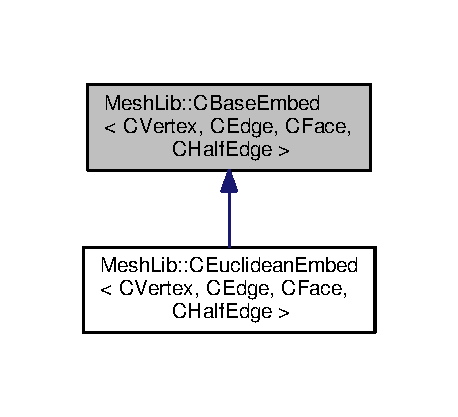
\includegraphics[width=220pt]{class_mesh_lib_1_1_c_base_embed__inherit__graph}
\end{center}
\end{figure}
\subsection*{Public Member Functions}
\begin{DoxyCompactItemize}
\item 
\hyperlink{class_mesh_lib_1_1_c_base_embed_ac6cfdbea469712b1d86d814e9bfae1a0}{C\+Base\+Embed} (C\+Ricci\+Flow\+Mesh$<$ \hyperlink{class_mesh_lib_1_1_c_vertex}{C\+Vertex}, \hyperlink{class_mesh_lib_1_1_c_edge}{C\+Edge}, \hyperlink{class_mesh_lib_1_1_c_face}{C\+Face}, \hyperlink{class_mesh_lib_1_1_c_half_edge}{C\+Half\+Edge} $>$ $\ast$p\+Mesh)
\begin{DoxyCompactList}\small\item\em C\+Embed constructor. \end{DoxyCompactList}\item 
\hyperlink{class_mesh_lib_1_1_c_base_embed_a97493bfd00df5af9048599c35f7722ef}{$\sim$\+C\+Base\+Embed} ()
\begin{DoxyCompactList}\small\item\em C\+Embed destructor. \end{DoxyCompactList}\item 
void \hyperlink{class_mesh_lib_1_1_c_base_embed_a5128819dbda9081bcaf0e4e75f82fa91}{\+\_\+embed} ()
\end{DoxyCompactItemize}
\subsection*{Protected Member Functions}
\begin{DoxyCompactItemize}
\item 
virtual void \hyperlink{class_mesh_lib_1_1_c_base_embed_a1a05d4cad7181da5a1ccc66265609f89}{\+\_\+embed\+\_\+first\+\_\+face} (\hyperlink{class_mesh_lib_1_1_c_face}{C\+Face} $\ast$head)=0
\item 
virtual void \hyperlink{class_mesh_lib_1_1_c_base_embed_a41a602699326b590a718570141923258}{\+\_\+embed\+\_\+face} (\hyperlink{class_mesh_lib_1_1_c_face}{C\+Face} $\ast$head)=0
\item 
void \hyperlink{class_mesh_lib_1_1_c_base_embed_ab064a0d24575758805edc7829b5e2d6e}{\+\_\+initialize} ()
\end{DoxyCompactItemize}
\subsection*{Protected Attributes}
\begin{DoxyCompactItemize}
\item 
C\+Ricci\+Flow\+Mesh$<$ \hyperlink{class_mesh_lib_1_1_c_vertex}{C\+Vertex}, \hyperlink{class_mesh_lib_1_1_c_edge}{C\+Edge}, \hyperlink{class_mesh_lib_1_1_c_face}{C\+Face}, \hyperlink{class_mesh_lib_1_1_c_half_edge}{C\+Half\+Edge} $>$ $\ast$ \hyperlink{class_mesh_lib_1_1_c_base_embed_a78bc5d476b39b3b3cb0d627de477d2f4}{m\+\_\+p\+Mesh}
\item 
std\+::queue$<$ \hyperlink{class_mesh_lib_1_1_c_face}{C\+Face} $\ast$ $>$ \hyperlink{class_mesh_lib_1_1_c_base_embed_a3ab9dc6044ded5990cd90643b99d8298}{m\+\_\+queue}
\end{DoxyCompactItemize}


\subsection{Detailed Description}
\subsubsection*{template$<$class C\+Vertex, class C\+Edge, class C\+Face, class C\+Half\+Edge$>$\\*
class Mesh\+Lib\+::\+C\+Base\+Embed$<$ C\+Vertex, C\+Edge, C\+Face, C\+Half\+Edge $>$}

\hyperlink{class_mesh_lib_1_1_c_base_embed}{C\+Base\+Embed} class. 

embed a mesh with canonical metric onto the canonical domain 

Definition at line 24 of file Base\+Embed.\+h.



\subsection{Constructor \& Destructor Documentation}
\index{Mesh\+Lib\+::\+C\+Base\+Embed@{Mesh\+Lib\+::\+C\+Base\+Embed}!C\+Base\+Embed@{C\+Base\+Embed}}
\index{C\+Base\+Embed@{C\+Base\+Embed}!Mesh\+Lib\+::\+C\+Base\+Embed@{Mesh\+Lib\+::\+C\+Base\+Embed}}
\subsubsection[{\texorpdfstring{C\+Base\+Embed(\+C\+Ricci\+Flow\+Mesh$<$ C\+Vertex, C\+Edge, C\+Face, C\+Half\+Edge $>$ $\ast$p\+Mesh)}{CBaseEmbed(CRicciFlowMesh< CVertex, CEdge, CFace, CHalfEdge > *pMesh)}}]{\setlength{\rightskip}{0pt plus 5cm}template$<$class C\+Vertex , class C\+Edge , class C\+Face , class C\+Half\+Edge $>$ {\bf Mesh\+Lib\+::\+C\+Base\+Embed}$<$ {\bf C\+Vertex}, {\bf C\+Edge}, {\bf C\+Face}, {\bf C\+Half\+Edge} $>$\+::{\bf C\+Base\+Embed} (
\begin{DoxyParamCaption}
\item[{C\+Ricci\+Flow\+Mesh$<$ {\bf C\+Vertex}, {\bf C\+Edge}, {\bf C\+Face}, {\bf C\+Half\+Edge} $>$ $\ast$}]{p\+Mesh}
\end{DoxyParamCaption}
)}\hypertarget{class_mesh_lib_1_1_c_base_embed_ac6cfdbea469712b1d86d814e9bfae1a0}{}\label{class_mesh_lib_1_1_c_base_embed_ac6cfdbea469712b1d86d814e9bfae1a0}


C\+Embed constructor. 



Definition at line 61 of file Base\+Embed.\+h.

\index{Mesh\+Lib\+::\+C\+Base\+Embed@{Mesh\+Lib\+::\+C\+Base\+Embed}!````~C\+Base\+Embed@{$\sim$\+C\+Base\+Embed}}
\index{````~C\+Base\+Embed@{$\sim$\+C\+Base\+Embed}!Mesh\+Lib\+::\+C\+Base\+Embed@{Mesh\+Lib\+::\+C\+Base\+Embed}}
\subsubsection[{\texorpdfstring{$\sim$\+C\+Base\+Embed()}{~CBaseEmbed()}}]{\setlength{\rightskip}{0pt plus 5cm}template$<$class C\+Vertex , class C\+Edge , class C\+Face , class C\+Half\+Edge $>$ {\bf Mesh\+Lib\+::\+C\+Base\+Embed}$<$ {\bf C\+Vertex}, {\bf C\+Edge}, {\bf C\+Face}, {\bf C\+Half\+Edge} $>$\+::$\sim${\bf C\+Base\+Embed} (
\begin{DoxyParamCaption}
{}
\end{DoxyParamCaption}
)\hspace{0.3cm}{\ttfamily [inline]}}\hypertarget{class_mesh_lib_1_1_c_base_embed_a97493bfd00df5af9048599c35f7722ef}{}\label{class_mesh_lib_1_1_c_base_embed_a97493bfd00df5af9048599c35f7722ef}


C\+Embed destructor. 



Definition at line 30 of file Base\+Embed.\+h.



\subsection{Member Function Documentation}
\index{Mesh\+Lib\+::\+C\+Base\+Embed@{Mesh\+Lib\+::\+C\+Base\+Embed}!\+\_\+embed@{\+\_\+embed}}
\index{\+\_\+embed@{\+\_\+embed}!Mesh\+Lib\+::\+C\+Base\+Embed@{Mesh\+Lib\+::\+C\+Base\+Embed}}
\subsubsection[{\texorpdfstring{\+\_\+embed()}{_embed()}}]{\setlength{\rightskip}{0pt plus 5cm}template$<$class C\+Vertex , class C\+Edge , class C\+Face , class C\+Half\+Edge $>$ void {\bf Mesh\+Lib\+::\+C\+Base\+Embed}$<$ {\bf C\+Vertex}, {\bf C\+Edge}, {\bf C\+Face}, {\bf C\+Half\+Edge} $>$\+::\+\_\+embed (
\begin{DoxyParamCaption}
{}
\end{DoxyParamCaption}
)}\hypertarget{class_mesh_lib_1_1_c_base_embed_a5128819dbda9081bcaf0e4e75f82fa91}{}\label{class_mesh_lib_1_1_c_base_embed_a5128819dbda9081bcaf0e4e75f82fa91}
\+\_\+embed the mesh 

Definition at line 109 of file Base\+Embed.\+h.

\index{Mesh\+Lib\+::\+C\+Base\+Embed@{Mesh\+Lib\+::\+C\+Base\+Embed}!\+\_\+embed\+\_\+face@{\+\_\+embed\+\_\+face}}
\index{\+\_\+embed\+\_\+face@{\+\_\+embed\+\_\+face}!Mesh\+Lib\+::\+C\+Base\+Embed@{Mesh\+Lib\+::\+C\+Base\+Embed}}
\subsubsection[{\texorpdfstring{\+\_\+embed\+\_\+face(\+C\+Face $\ast$head)=0}{_embed_face(CFace *head)=0}}]{\setlength{\rightskip}{0pt plus 5cm}template$<$class C\+Vertex , class C\+Edge , class C\+Face , class C\+Half\+Edge $>$ virtual void {\bf Mesh\+Lib\+::\+C\+Base\+Embed}$<$ {\bf C\+Vertex}, {\bf C\+Edge}, {\bf C\+Face}, {\bf C\+Half\+Edge} $>$\+::\+\_\+embed\+\_\+face (
\begin{DoxyParamCaption}
\item[{{\bf C\+Face} $\ast$}]{head}
\end{DoxyParamCaption}
)\hspace{0.3cm}{\ttfamily [protected]}, {\ttfamily [pure virtual]}}\hypertarget{class_mesh_lib_1_1_c_base_embed_a41a602699326b590a718570141923258}{}\label{class_mesh_lib_1_1_c_base_embed_a41a602699326b590a718570141923258}


Implemented in \hyperlink{class_mesh_lib_1_1_c_euclidean_embed_aa77b6c218a33dbb01bc1eb5aad444c32}{Mesh\+Lib\+::\+C\+Euclidean\+Embed$<$ C\+Vertex, C\+Edge, C\+Face, C\+Half\+Edge $>$}.

\index{Mesh\+Lib\+::\+C\+Base\+Embed@{Mesh\+Lib\+::\+C\+Base\+Embed}!\+\_\+embed\+\_\+first\+\_\+face@{\+\_\+embed\+\_\+first\+\_\+face}}
\index{\+\_\+embed\+\_\+first\+\_\+face@{\+\_\+embed\+\_\+first\+\_\+face}!Mesh\+Lib\+::\+C\+Base\+Embed@{Mesh\+Lib\+::\+C\+Base\+Embed}}
\subsubsection[{\texorpdfstring{\+\_\+embed\+\_\+first\+\_\+face(\+C\+Face $\ast$head)=0}{_embed_first_face(CFace *head)=0}}]{\setlength{\rightskip}{0pt plus 5cm}template$<$class C\+Vertex , class C\+Edge , class C\+Face , class C\+Half\+Edge $>$ virtual void {\bf Mesh\+Lib\+::\+C\+Base\+Embed}$<$ {\bf C\+Vertex}, {\bf C\+Edge}, {\bf C\+Face}, {\bf C\+Half\+Edge} $>$\+::\+\_\+embed\+\_\+first\+\_\+face (
\begin{DoxyParamCaption}
\item[{{\bf C\+Face} $\ast$}]{head}
\end{DoxyParamCaption}
)\hspace{0.3cm}{\ttfamily [protected]}, {\ttfamily [pure virtual]}}\hypertarget{class_mesh_lib_1_1_c_base_embed_a1a05d4cad7181da5a1ccc66265609f89}{}\label{class_mesh_lib_1_1_c_base_embed_a1a05d4cad7181da5a1ccc66265609f89}
embed the first face 
\begin{DoxyParams}{Parameters}
{\em head} & the first face \\
\hline
\end{DoxyParams}


Implemented in \hyperlink{class_mesh_lib_1_1_c_euclidean_embed_a6910ac47a9c2b101b8dca4049a533141}{Mesh\+Lib\+::\+C\+Euclidean\+Embed$<$ C\+Vertex, C\+Edge, C\+Face, C\+Half\+Edge $>$}.

\index{Mesh\+Lib\+::\+C\+Base\+Embed@{Mesh\+Lib\+::\+C\+Base\+Embed}!\+\_\+initialize@{\+\_\+initialize}}
\index{\+\_\+initialize@{\+\_\+initialize}!Mesh\+Lib\+::\+C\+Base\+Embed@{Mesh\+Lib\+::\+C\+Base\+Embed}}
\subsubsection[{\texorpdfstring{\+\_\+initialize()}{_initialize()}}]{\setlength{\rightskip}{0pt plus 5cm}template$<$class C\+Vertex , class C\+Edge , class C\+Face , class C\+Half\+Edge $>$ void {\bf Mesh\+Lib\+::\+C\+Base\+Embed}$<$ {\bf C\+Vertex}, {\bf C\+Edge}, {\bf C\+Face}, {\bf C\+Half\+Edge} $>$\+::\+\_\+initialize (
\begin{DoxyParamCaption}
{}
\end{DoxyParamCaption}
)\hspace{0.3cm}{\ttfamily [protected]}}\hypertarget{class_mesh_lib_1_1_c_base_embed_ab064a0d24575758805edc7829b5e2d6e}{}\label{class_mesh_lib_1_1_c_base_embed_ab064a0d24575758805edc7829b5e2d6e}
initialization 

Definition at line 71 of file Base\+Embed.\+h.



\subsection{Member Data Documentation}
\index{Mesh\+Lib\+::\+C\+Base\+Embed@{Mesh\+Lib\+::\+C\+Base\+Embed}!m\+\_\+p\+Mesh@{m\+\_\+p\+Mesh}}
\index{m\+\_\+p\+Mesh@{m\+\_\+p\+Mesh}!Mesh\+Lib\+::\+C\+Base\+Embed@{Mesh\+Lib\+::\+C\+Base\+Embed}}
\subsubsection[{\texorpdfstring{m\+\_\+p\+Mesh}{m_pMesh}}]{\setlength{\rightskip}{0pt plus 5cm}template$<$class C\+Vertex , class C\+Edge , class C\+Face , class C\+Half\+Edge $>$ C\+Ricci\+Flow\+Mesh$<${\bf C\+Vertex},{\bf C\+Edge},{\bf C\+Face},{\bf C\+Half\+Edge}$>$$\ast$ {\bf Mesh\+Lib\+::\+C\+Base\+Embed}$<$ {\bf C\+Vertex}, {\bf C\+Edge}, {\bf C\+Face}, {\bf C\+Half\+Edge} $>$\+::m\+\_\+p\+Mesh\hspace{0.3cm}{\ttfamily [protected]}}\hypertarget{class_mesh_lib_1_1_c_base_embed_a78bc5d476b39b3b3cb0d627de477d2f4}{}\label{class_mesh_lib_1_1_c_base_embed_a78bc5d476b39b3b3cb0d627de477d2f4}
the mesh to be embedded 

Definition at line 51 of file Base\+Embed.\+h.

\index{Mesh\+Lib\+::\+C\+Base\+Embed@{Mesh\+Lib\+::\+C\+Base\+Embed}!m\+\_\+queue@{m\+\_\+queue}}
\index{m\+\_\+queue@{m\+\_\+queue}!Mesh\+Lib\+::\+C\+Base\+Embed@{Mesh\+Lib\+::\+C\+Base\+Embed}}
\subsubsection[{\texorpdfstring{m\+\_\+queue}{m_queue}}]{\setlength{\rightskip}{0pt plus 5cm}template$<$class C\+Vertex , class C\+Edge , class C\+Face , class C\+Half\+Edge $>$ std\+::queue$<${\bf C\+Face}$\ast$$>$ {\bf Mesh\+Lib\+::\+C\+Base\+Embed}$<$ {\bf C\+Vertex}, {\bf C\+Edge}, {\bf C\+Face}, {\bf C\+Half\+Edge} $>$\+::m\+\_\+queue\hspace{0.3cm}{\ttfamily [protected]}}\hypertarget{class_mesh_lib_1_1_c_base_embed_a3ab9dc6044ded5990cd90643b99d8298}{}\label{class_mesh_lib_1_1_c_base_embed_a3ab9dc6044ded5990cd90643b99d8298}
queue of faces 

Definition at line 54 of file Base\+Embed.\+h.



The documentation for this class was generated from the following file\+:\begin{DoxyCompactItemize}
\item 
Mesh\+Lib/algorithm/\+Riemannian/\+Ricci\+Flow/\hyperlink{_base_embed_8h}{Base\+Embed.\+h}\end{DoxyCompactItemize}

\hypertarget{class_mesh_lib_1_1_c_base_mesh}{}\section{Mesh\+Lib\+:\+:C\+Base\+Mesh$<$ C\+Vertex, C\+Edge, C\+Face, C\+Half\+Edge $>$ Class Template Reference}
\label{class_mesh_lib_1_1_c_base_mesh}\index{Mesh\+Lib\+::\+C\+Base\+Mesh$<$ C\+Vertex, C\+Edge, C\+Face, C\+Half\+Edge $>$@{Mesh\+Lib\+::\+C\+Base\+Mesh$<$ C\+Vertex, C\+Edge, C\+Face, C\+Half\+Edge $>$}}


\hyperlink{class_mesh_lib_1_1_c_base_mesh}{C\+Base\+Mesh}, base class for all types of mesh classes.  




{\ttfamily \#include $<$Base\+Mesh.\+h$>$}

\subsection*{Public Types}
\begin{DoxyCompactItemize}
\item 
typedef \hyperlink{class_mesh_lib_1_1_c_vertex}{C\+Vertex} $\ast$ \hyperlink{class_mesh_lib_1_1_c_base_mesh_adcf412e8267910b50f3145d6416947da}{t\+Vertex}
\item 
typedef \hyperlink{class_mesh_lib_1_1_c_half_edge}{C\+Half\+Edge} $\ast$ \hyperlink{class_mesh_lib_1_1_c_base_mesh_a30024aa977abb5ab248e7c87ba1ec109}{t\+Half\+Edge}
\item 
typedef \hyperlink{class_mesh_lib_1_1_c_edge}{C\+Edge} $\ast$ \hyperlink{class_mesh_lib_1_1_c_base_mesh_a966f6321c2cf92b849e77b931a36821b}{t\+Edge}
\item 
typedef \hyperlink{class_mesh_lib_1_1_c_face}{C\+Face} $\ast$ \hyperlink{class_mesh_lib_1_1_c_base_mesh_ad231546551e85dffb41c9aa9bcf5b86b}{t\+Face}
\end{DoxyCompactItemize}
\subsection*{Public Member Functions}
\begin{DoxyCompactItemize}
\item 
\hyperlink{class_mesh_lib_1_1_c_base_mesh_ac0fb8b8bec22dcfc33d694bae1905e9e}{C\+Base\+Mesh} ()
\item 
\hyperlink{class_mesh_lib_1_1_c_base_mesh_a875ca1255924a0ce68566150d4c55e76}{$\sim$\+C\+Base\+Mesh} ()
\item 
void \hyperlink{class_mesh_lib_1_1_c_base_mesh_a65338968dc92c9d326956a9a60d08f35}{copy} (\hyperlink{class_mesh_lib_1_1_c_base_mesh}{C\+Base\+Mesh} \&mesh)
\item 
void \hyperlink{class_mesh_lib_1_1_c_base_mesh_ad711e992ab1cd7371690eba2b6292b35}{read\+\_\+obj} (const char $\ast$filename)
\item 
void \hyperlink{class_mesh_lib_1_1_c_base_mesh_af885e691fce7e793d5d4185ea286d1cc}{write\+\_\+obj} (const char $\ast$output)
\item 
void \hyperlink{class_mesh_lib_1_1_c_base_mesh_ace7e07c6b5f0d07cdfda11d3f73139f4}{read\+\_\+m} (const char $\ast$input)
\item 
void \hyperlink{class_mesh_lib_1_1_c_base_mesh_aac9e4fdd74de34f44e8ac7afad00c322}{write\+\_\+m} (const char $\ast$output)
\item 
void \hyperlink{class_mesh_lib_1_1_c_base_mesh_a15db6845a5ce5460a92a6afb0fcd1a31}{read\+\_\+off} (const char $\ast$input)
\item 
void \hyperlink{class_mesh_lib_1_1_c_base_mesh_a1ec12eff25a713eb43d2cdef1b452743}{write\+\_\+off} (const char $\ast$output)
\item 
int \hyperlink{class_mesh_lib_1_1_c_base_mesh_a180ba1fbde1e68a4a2201928e6573dc7}{num\+Vertices} ()
\item 
int \hyperlink{class_mesh_lib_1_1_c_base_mesh_a59246eb0edbe1ad11f0e6ecb41444135}{num\+Edges} ()
\item 
int \hyperlink{class_mesh_lib_1_1_c_base_mesh_ac750e49625e3ebbc50a135f77cbbdf87}{num\+Faces} ()
\item 
bool \hyperlink{class_mesh_lib_1_1_c_base_mesh_a74e917019ff789ac7e4e402de81cbe94}{is\+Boundary} (\hyperlink{class_mesh_lib_1_1_c_base_mesh_adcf412e8267910b50f3145d6416947da}{t\+Vertex} v)
\item 
bool \hyperlink{class_mesh_lib_1_1_c_base_mesh_a9cd94b0e1dd28c2aecce5c15975e0bd8}{is\+Boundary} (\hyperlink{class_mesh_lib_1_1_c_base_mesh_a966f6321c2cf92b849e77b931a36821b}{t\+Edge} e)
\item 
bool \hyperlink{class_mesh_lib_1_1_c_base_mesh_a8d60d481e391e80b3ef710811fe83352}{is\+Boundary} (\hyperlink{class_mesh_lib_1_1_c_base_mesh_a30024aa977abb5ab248e7c87ba1ec109}{t\+Half\+Edge} he)
\item 
\hyperlink{class_mesh_lib_1_1_c_base_mesh_adcf412e8267910b50f3145d6416947da}{t\+Vertex} \hyperlink{class_mesh_lib_1_1_c_base_mesh_af03a301faaed2e2ea23ddca3b96a8b23}{id\+Vertex} (int id)
\item 
int \hyperlink{class_mesh_lib_1_1_c_base_mesh_a5f2f3d6715095a364f390321868aaa8a}{vertex\+Id} (\hyperlink{class_mesh_lib_1_1_c_base_mesh_adcf412e8267910b50f3145d6416947da}{t\+Vertex} v)
\item 
\hyperlink{class_mesh_lib_1_1_c_base_mesh_ad231546551e85dffb41c9aa9bcf5b86b}{t\+Face} \hyperlink{class_mesh_lib_1_1_c_base_mesh_aad0fd30815bc0a4b414e9ad7b9d6c81f}{id\+Face} (int id)
\item 
int \hyperlink{class_mesh_lib_1_1_c_base_mesh_a721b0f334a34d5e6e23b99ba186f0606}{face\+Id} (\hyperlink{class_mesh_lib_1_1_c_base_mesh_ad231546551e85dffb41c9aa9bcf5b86b}{t\+Face} f)
\item 
\hyperlink{class_mesh_lib_1_1_c_base_mesh_a966f6321c2cf92b849e77b931a36821b}{t\+Edge} \hyperlink{class_mesh_lib_1_1_c_base_mesh_ae8a58acc899cab99f651b0845250d311}{vertex\+Edge} (\hyperlink{class_mesh_lib_1_1_c_base_mesh_adcf412e8267910b50f3145d6416947da}{t\+Vertex} v0, \hyperlink{class_mesh_lib_1_1_c_base_mesh_adcf412e8267910b50f3145d6416947da}{t\+Vertex} v1)
\item 
\hyperlink{class_mesh_lib_1_1_c_base_mesh_a30024aa977abb5ab248e7c87ba1ec109}{t\+Half\+Edge} \hyperlink{class_mesh_lib_1_1_c_base_mesh_ad43e40c6eef135e91d792ed9f4dfbccf}{vertex\+Halfedge} (\hyperlink{class_mesh_lib_1_1_c_base_mesh_adcf412e8267910b50f3145d6416947da}{t\+Vertex} v0, \hyperlink{class_mesh_lib_1_1_c_base_mesh_adcf412e8267910b50f3145d6416947da}{t\+Vertex} v1)
\item 
\hyperlink{class_mesh_lib_1_1_c_base_mesh_a30024aa977abb5ab248e7c87ba1ec109}{t\+Half\+Edge} \hyperlink{class_mesh_lib_1_1_c_base_mesh_a94ac4a6222c7ec036d586b1beb5c81d6}{corner} (\hyperlink{class_mesh_lib_1_1_c_base_mesh_adcf412e8267910b50f3145d6416947da}{t\+Vertex} v, \hyperlink{class_mesh_lib_1_1_c_base_mesh_ad231546551e85dffb41c9aa9bcf5b86b}{t\+Face} f)
\item 
\hyperlink{class_mesh_lib_1_1_c_base_mesh_ad231546551e85dffb41c9aa9bcf5b86b}{t\+Face} \hyperlink{class_mesh_lib_1_1_c_base_mesh_ad244041d5d03f443128eec0c589e6a5c}{halfedge\+Face} (\hyperlink{class_mesh_lib_1_1_c_base_mesh_a30024aa977abb5ab248e7c87ba1ec109}{t\+Half\+Edge} he)
\item 
\hyperlink{class_mesh_lib_1_1_c_base_mesh_adcf412e8267910b50f3145d6416947da}{t\+Vertex} \hyperlink{class_mesh_lib_1_1_c_base_mesh_ab306584de9fde74de2038c0b0113d0a0}{halfedge\+Vertex} (\hyperlink{class_mesh_lib_1_1_c_base_mesh_a30024aa977abb5ab248e7c87ba1ec109}{t\+Half\+Edge} he)
\item 
\hyperlink{class_mesh_lib_1_1_c_base_mesh_adcf412e8267910b50f3145d6416947da}{t\+Vertex} \hyperlink{class_mesh_lib_1_1_c_base_mesh_a019148ba8fcdc951366bb297f7cf706d}{halfedge\+Target} (\hyperlink{class_mesh_lib_1_1_c_base_mesh_a30024aa977abb5ab248e7c87ba1ec109}{t\+Half\+Edge} he)
\item 
\hyperlink{class_mesh_lib_1_1_c_base_mesh_adcf412e8267910b50f3145d6416947da}{t\+Vertex} \hyperlink{class_mesh_lib_1_1_c_base_mesh_aa3e98fc14c2dae20fd4fada65c5d13a2}{halfedge\+Source} (\hyperlink{class_mesh_lib_1_1_c_base_mesh_a30024aa977abb5ab248e7c87ba1ec109}{t\+Half\+Edge} he)
\item 
\hyperlink{class_mesh_lib_1_1_c_base_mesh_a30024aa977abb5ab248e7c87ba1ec109}{t\+Half\+Edge} \hyperlink{class_mesh_lib_1_1_c_base_mesh_a172ab9124d1c0236a66e104fe1cce404}{halfedge\+Next} (\hyperlink{class_mesh_lib_1_1_c_base_mesh_a30024aa977abb5ab248e7c87ba1ec109}{t\+Half\+Edge} he)
\item 
\hyperlink{class_mesh_lib_1_1_c_base_mesh_a30024aa977abb5ab248e7c87ba1ec109}{t\+Half\+Edge} \hyperlink{class_mesh_lib_1_1_c_base_mesh_a9d89bff17b86a5d8f0dc13f4eb7f5b6f}{halfedge\+Prev} (\hyperlink{class_mesh_lib_1_1_c_base_mesh_a30024aa977abb5ab248e7c87ba1ec109}{t\+Half\+Edge} he)
\item 
\hyperlink{class_mesh_lib_1_1_c_base_mesh_a30024aa977abb5ab248e7c87ba1ec109}{t\+Half\+Edge} \hyperlink{class_mesh_lib_1_1_c_base_mesh_a4905fc3ff11c836e07395dd424d37ece}{halfedge\+Sym} (\hyperlink{class_mesh_lib_1_1_c_base_mesh_a30024aa977abb5ab248e7c87ba1ec109}{t\+Half\+Edge} he)
\item 
\hyperlink{class_mesh_lib_1_1_c_base_mesh_a966f6321c2cf92b849e77b931a36821b}{t\+Edge} \hyperlink{class_mesh_lib_1_1_c_base_mesh_ada3fa889304e08af51bc8734512ab38e}{halfedge\+Edge} (\hyperlink{class_mesh_lib_1_1_c_base_mesh_a30024aa977abb5ab248e7c87ba1ec109}{t\+Half\+Edge} he)
\item 
\hyperlink{class_mesh_lib_1_1_c_base_mesh_a30024aa977abb5ab248e7c87ba1ec109}{t\+Half\+Edge} \hyperlink{class_mesh_lib_1_1_c_base_mesh_a46a10c439e6a7c13f0dec5bd62ce1565}{vertex\+Halfedge} (\hyperlink{class_mesh_lib_1_1_c_base_mesh_adcf412e8267910b50f3145d6416947da}{t\+Vertex} v)
\item 
std\+::list$<$ \hyperlink{class_mesh_lib_1_1_c_base_mesh_a966f6321c2cf92b849e77b931a36821b}{t\+Edge} $>$ \& \hyperlink{class_mesh_lib_1_1_c_base_mesh_a73ddf93eff3bcb04f5657bb858403cc1}{vertex\+Edges} (\hyperlink{class_mesh_lib_1_1_c_base_mesh_adcf412e8267910b50f3145d6416947da}{t\+Vertex} v)
\item 
\hyperlink{class_mesh_lib_1_1_c_base_mesh_adcf412e8267910b50f3145d6416947da}{t\+Vertex} \hyperlink{class_mesh_lib_1_1_c_base_mesh_ae5e25339a32fa919bb4c3600b03435f9}{edge\+Vertex1} (\hyperlink{class_mesh_lib_1_1_c_base_mesh_a966f6321c2cf92b849e77b931a36821b}{t\+Edge} e)
\item 
\hyperlink{class_mesh_lib_1_1_c_base_mesh_adcf412e8267910b50f3145d6416947da}{t\+Vertex} \hyperlink{class_mesh_lib_1_1_c_base_mesh_a348d1cc713885bf04be5684727dcbf21}{edge\+Vertex2} (\hyperlink{class_mesh_lib_1_1_c_base_mesh_a966f6321c2cf92b849e77b931a36821b}{t\+Edge} e)
\item 
\hyperlink{class_mesh_lib_1_1_c_base_mesh_ad231546551e85dffb41c9aa9bcf5b86b}{t\+Face} \hyperlink{class_mesh_lib_1_1_c_base_mesh_aa00d7192146f94c4853fb1b660a449c6}{edge\+Face1} (\hyperlink{class_mesh_lib_1_1_c_base_mesh_a966f6321c2cf92b849e77b931a36821b}{t\+Edge} e)
\item 
\hyperlink{class_mesh_lib_1_1_c_base_mesh_ad231546551e85dffb41c9aa9bcf5b86b}{t\+Face} \hyperlink{class_mesh_lib_1_1_c_base_mesh_ab52850e9a6bb778f3372b925d01e2783}{edge\+Face2} (\hyperlink{class_mesh_lib_1_1_c_base_mesh_a966f6321c2cf92b849e77b931a36821b}{t\+Edge} e)
\item 
\hyperlink{class_mesh_lib_1_1_c_base_mesh_a30024aa977abb5ab248e7c87ba1ec109}{t\+Half\+Edge} \hyperlink{class_mesh_lib_1_1_c_base_mesh_ab1bc4850fcc8e74cfdf16560ecb9558a}{edge\+Halfedge} (\hyperlink{class_mesh_lib_1_1_c_base_mesh_a966f6321c2cf92b849e77b931a36821b}{t\+Edge} e, int id)
\item 
\hyperlink{class_mesh_lib_1_1_c_base_mesh_a30024aa977abb5ab248e7c87ba1ec109}{t\+Half\+Edge} \hyperlink{class_mesh_lib_1_1_c_base_mesh_a24655b5a0c6cba60c236c84def777e9a}{face\+Halfedge} (\hyperlink{class_mesh_lib_1_1_c_base_mesh_ad231546551e85dffb41c9aa9bcf5b86b}{t\+Face} f)
\item 
\hyperlink{class_mesh_lib_1_1_c_base_mesh_a30024aa977abb5ab248e7c87ba1ec109}{t\+Half\+Edge} \hyperlink{class_mesh_lib_1_1_c_base_mesh_a170cd5aafa0925c710c0d770789b2f6d}{vertex\+Most\+Clw\+Out\+Half\+Edge} (\hyperlink{class_mesh_lib_1_1_c_base_mesh_adcf412e8267910b50f3145d6416947da}{t\+Vertex} v)
\item 
\hyperlink{class_mesh_lib_1_1_c_base_mesh_a30024aa977abb5ab248e7c87ba1ec109}{t\+Half\+Edge} \hyperlink{class_mesh_lib_1_1_c_base_mesh_ac0a1fd4394382d87004048cff63e2efe}{vertex\+Next\+Ccw\+Out\+Half\+Edge} (\hyperlink{class_mesh_lib_1_1_c_base_mesh_a30024aa977abb5ab248e7c87ba1ec109}{t\+Half\+Edge} he)
\item 
\hyperlink{class_mesh_lib_1_1_c_base_mesh_a30024aa977abb5ab248e7c87ba1ec109}{t\+Half\+Edge} \hyperlink{class_mesh_lib_1_1_c_base_mesh_a90c1bfc4bc7d1467c1d36dbc792d5481}{vertex\+Most\+Ccw\+Out\+Half\+Edge} (\hyperlink{class_mesh_lib_1_1_c_base_mesh_adcf412e8267910b50f3145d6416947da}{t\+Vertex} v)
\item 
\hyperlink{class_mesh_lib_1_1_c_base_mesh_a30024aa977abb5ab248e7c87ba1ec109}{t\+Half\+Edge} \hyperlink{class_mesh_lib_1_1_c_base_mesh_af2f1696c5e66668c8b1f3fe98b4c5d92}{vertex\+Next\+Clw\+Out\+Half\+Edge} (\hyperlink{class_mesh_lib_1_1_c_base_mesh_a30024aa977abb5ab248e7c87ba1ec109}{t\+Half\+Edge} he)
\item 
\hyperlink{class_mesh_lib_1_1_c_base_mesh_a30024aa977abb5ab248e7c87ba1ec109}{t\+Half\+Edge} \hyperlink{class_mesh_lib_1_1_c_base_mesh_a3966eec3d8d8a301bfaac27e380210fc}{vertex\+Most\+Clw\+In\+Half\+Edge} (\hyperlink{class_mesh_lib_1_1_c_base_mesh_adcf412e8267910b50f3145d6416947da}{t\+Vertex} v)
\item 
\hyperlink{class_mesh_lib_1_1_c_base_mesh_a30024aa977abb5ab248e7c87ba1ec109}{t\+Half\+Edge} \hyperlink{class_mesh_lib_1_1_c_base_mesh_a721933757b5348b4c251d519e95a9a96}{vertex\+Next\+Ccw\+In\+Half\+Edge} (\hyperlink{class_mesh_lib_1_1_c_base_mesh_a30024aa977abb5ab248e7c87ba1ec109}{t\+Half\+Edge} he)
\item 
\hyperlink{class_mesh_lib_1_1_c_base_mesh_a30024aa977abb5ab248e7c87ba1ec109}{t\+Half\+Edge} \hyperlink{class_mesh_lib_1_1_c_base_mesh_a201002431101172f57da7ec748a2770e}{vertex\+Most\+Ccw\+In\+Half\+Edge} (\hyperlink{class_mesh_lib_1_1_c_base_mesh_adcf412e8267910b50f3145d6416947da}{t\+Vertex} v)
\item 
\hyperlink{class_mesh_lib_1_1_c_base_mesh_a30024aa977abb5ab248e7c87ba1ec109}{t\+Half\+Edge} \hyperlink{class_mesh_lib_1_1_c_base_mesh_a29d3d0c0a41b3e54e777b9546cbd88f6}{vertex\+Next\+Clw\+In\+Half\+Edge} (\hyperlink{class_mesh_lib_1_1_c_base_mesh_a30024aa977abb5ab248e7c87ba1ec109}{t\+Half\+Edge} he)
\item 
\hyperlink{class_mesh_lib_1_1_c_base_mesh_a30024aa977abb5ab248e7c87ba1ec109}{t\+Half\+Edge} \hyperlink{class_mesh_lib_1_1_c_base_mesh_a093a262a9ac1648f4a9071b46858634f}{face\+Most\+Clw\+Half\+Edge} (\hyperlink{class_mesh_lib_1_1_c_base_mesh_ad231546551e85dffb41c9aa9bcf5b86b}{t\+Face} face)
\item 
\hyperlink{class_mesh_lib_1_1_c_base_mesh_a30024aa977abb5ab248e7c87ba1ec109}{t\+Half\+Edge} \hyperlink{class_mesh_lib_1_1_c_base_mesh_ae935733ecd2d03ea094f93e5e174c775}{face\+Most\+Ccw\+Half\+Edge} (\hyperlink{class_mesh_lib_1_1_c_base_mesh_ad231546551e85dffb41c9aa9bcf5b86b}{t\+Face} face)
\item 
\hyperlink{class_mesh_lib_1_1_c_base_mesh_a30024aa977abb5ab248e7c87ba1ec109}{t\+Half\+Edge} \hyperlink{class_mesh_lib_1_1_c_base_mesh_a1ab17a733e28d417106f6e32be8a80cf}{face\+Next\+Ccw\+Half\+Edge} (\hyperlink{class_mesh_lib_1_1_c_base_mesh_a30024aa977abb5ab248e7c87ba1ec109}{t\+Half\+Edge} he)
\item 
\hyperlink{class_mesh_lib_1_1_c_base_mesh_a30024aa977abb5ab248e7c87ba1ec109}{t\+Half\+Edge} \hyperlink{class_mesh_lib_1_1_c_base_mesh_af9fef8808ee51bfa9c3d043bde7b3db4}{face\+Next\+Clw\+Half\+Edge} (\hyperlink{class_mesh_lib_1_1_c_base_mesh_a30024aa977abb5ab248e7c87ba1ec109}{t\+Half\+Edge} he)
\item 
double \hyperlink{class_mesh_lib_1_1_c_base_mesh_a2f1e00892d9f3c970937a2c20196d225}{edge\+Length} (\hyperlink{class_mesh_lib_1_1_c_base_mesh_a966f6321c2cf92b849e77b931a36821b}{t\+Edge} e)
\item 
std\+::list$<$ \hyperlink{class_mesh_lib_1_1_c_base_mesh_a966f6321c2cf92b849e77b931a36821b}{t\+Edge} $>$ \& \hyperlink{class_mesh_lib_1_1_c_base_mesh_ac4b7febcad1cc9a1539d517fb3d3c97a}{edges} ()
\item 
std\+::list$<$ \hyperlink{class_mesh_lib_1_1_c_base_mesh_ad231546551e85dffb41c9aa9bcf5b86b}{t\+Face} $>$ \& \hyperlink{class_mesh_lib_1_1_c_base_mesh_a8eb590668265fbcfe64f60567580c80f}{faces} ()
\item 
std\+::list$<$ \hyperlink{class_mesh_lib_1_1_c_base_mesh_adcf412e8267910b50f3145d6416947da}{t\+Vertex} $>$ \& \hyperlink{class_mesh_lib_1_1_c_base_mesh_a28d9bd75c518e0e5f4c9fab50008b8aa}{vertices} ()
\item 
\hyperlink{class_mesh_lib_1_1_c_base_mesh_adcf412e8267910b50f3145d6416947da}{t\+Vertex} \hyperlink{class_mesh_lib_1_1_c_base_mesh_a04ee0f997dd274fdcf5ba6bc7b979569}{create\+Vertex} (int id=0)
\item 
\hyperlink{class_mesh_lib_1_1_c_base_mesh_a966f6321c2cf92b849e77b931a36821b}{t\+Edge} \hyperlink{class_mesh_lib_1_1_c_base_mesh_a24b4f0bd948452d506631015deb704df}{create\+Edge} (\hyperlink{class_mesh_lib_1_1_c_base_mesh_adcf412e8267910b50f3145d6416947da}{t\+Vertex} v1, \hyperlink{class_mesh_lib_1_1_c_base_mesh_adcf412e8267910b50f3145d6416947da}{t\+Vertex} v2)
\item 
\hyperlink{class_mesh_lib_1_1_c_base_mesh_ad231546551e85dffb41c9aa9bcf5b86b}{t\+Face} \hyperlink{class_mesh_lib_1_1_c_base_mesh_a5c1a9a5b45a58d766a664595f8c799b1}{create\+Face} (\hyperlink{class_mesh_lib_1_1_c_base_mesh_adcf412e8267910b50f3145d6416947da}{t\+Vertex} v\mbox{[}$\,$\mbox{]}, int id)
\item 
\hyperlink{class_mesh_lib_1_1_c_base_mesh_ad231546551e85dffb41c9aa9bcf5b86b}{t\+Face} \hyperlink{class_mesh_lib_1_1_c_base_mesh_a2ae791035daa07ac116913aa6866e990}{create\+Face} (std\+::vector$<$ \hyperlink{class_mesh_lib_1_1_c_base_mesh_adcf412e8267910b50f3145d6416947da}{t\+Vertex} $>$ \&v, int id)
\item 
void \hyperlink{class_mesh_lib_1_1_c_base_mesh_a1a037d32457d70216d0885c31a2d889a}{delete\+Face} (\hyperlink{class_mesh_lib_1_1_c_base_mesh_ad231546551e85dffb41c9aa9bcf5b86b}{t\+Face} p\+Face)
\item 
void \hyperlink{class_mesh_lib_1_1_c_base_mesh_a7f7c5053e7254f0b3a9ed4869848885f}{label\+Boundary} (void)
\end{DoxyCompactItemize}
\subsection*{Public Attributes}
\begin{DoxyCompactItemize}
\item 
bool \hyperlink{class_mesh_lib_1_1_c_base_mesh_a36ba9fb8f3b289de348f1133ee6ab4bb}{m\+\_\+with\+\_\+texture}
\item 
bool \hyperlink{class_mesh_lib_1_1_c_base_mesh_a105ddccad80953028cc54cd317dee8a4}{m\+\_\+with\+\_\+normal}
\end{DoxyCompactItemize}
\subsection*{Static Public Attributes}
\begin{DoxyCompactItemize}
\item 
static unsigned long long \hyperlink{class_mesh_lib_1_1_c_base_mesh_a09dbf8905e5b0dbe3c8353070f83ae81}{m\+\_\+input\+\_\+traits}
\item 
static unsigned long long \hyperlink{class_mesh_lib_1_1_c_base_mesh_af1a7720a0b51675ac91cc8c00d1959a3}{m\+\_\+output\+\_\+traits}
\end{DoxyCompactItemize}
\subsection*{Protected Attributes}
\begin{DoxyCompactItemize}
\item 
std\+::list$<$ \hyperlink{class_mesh_lib_1_1_c_base_mesh_a966f6321c2cf92b849e77b931a36821b}{t\+Edge} $>$ \hyperlink{class_mesh_lib_1_1_c_base_mesh_a5986476cf61a1ea5b5932f33302b6c10}{m\+\_\+edges}
\item 
std\+::list$<$ \hyperlink{class_mesh_lib_1_1_c_base_mesh_adcf412e8267910b50f3145d6416947da}{t\+Vertex} $>$ \hyperlink{class_mesh_lib_1_1_c_base_mesh_a5738a63ce99209aa5085982ecc9ba50a}{m\+\_\+verts}
\item 
std\+::list$<$ \hyperlink{class_mesh_lib_1_1_c_base_mesh_ad231546551e85dffb41c9aa9bcf5b86b}{t\+Face} $>$ \hyperlink{class_mesh_lib_1_1_c_base_mesh_a4699846e3f577e064c3b871183d8ba0a}{m\+\_\+faces}
\item 
std\+::map$<$ int, \hyperlink{class_mesh_lib_1_1_c_base_mesh_adcf412e8267910b50f3145d6416947da}{t\+Vertex} $>$ \hyperlink{class_mesh_lib_1_1_c_base_mesh_ad92d530f9eacd1eb2adef1770fd0ff80}{m\+\_\+map\+\_\+vert}
\item 
std\+::map$<$ int, \hyperlink{class_mesh_lib_1_1_c_base_mesh_ad231546551e85dffb41c9aa9bcf5b86b}{t\+Face} $>$ \hyperlink{class_mesh_lib_1_1_c_base_mesh_afdcd24f68c0ab83a6b172a64753b7482}{m\+\_\+map\+\_\+face}
\end{DoxyCompactItemize}


\subsection{Detailed Description}
\subsubsection*{template$<$class C\+Vertex, class C\+Edge, class C\+Face, class C\+Half\+Edge$>$\\*
class Mesh\+Lib\+::\+C\+Base\+Mesh$<$ C\+Vertex, C\+Edge, C\+Face, C\+Half\+Edge $>$}

\hyperlink{class_mesh_lib_1_1_c_base_mesh}{C\+Base\+Mesh}, base class for all types of mesh classes. 

This is the fundamental class for meshes. It includes a list of vertices, a list of edges, a list of faces. All the geometric objects are connected by pointers, vertex, edge, face are connected by halfedges. The mesh class has file IO functionalities, supporting .obj, .m and .off file formats. It offers Euler operators, each geometric primative can access its neighbors freely.


\begin{DoxyTemplParams}{Template Parameters}
{\em \hyperlink{class_mesh_lib_1_1_c_vertex}{C\+Vertex}} & vertex class, derived from \hyperlink{class_mesh_lib_1_1_c_vertex}{Mesh\+Lib\+::\+C\+Vertex} class \\
\hline
{\em \hyperlink{class_mesh_lib_1_1_c_edge}{C\+Edge}} & edge class, derived from \hyperlink{class_mesh_lib_1_1_c_edge}{Mesh\+Lib\+::\+C\+Edge} class \\
\hline
{\em \hyperlink{class_mesh_lib_1_1_c_face}{C\+Face}} & face class, derived from \hyperlink{class_mesh_lib_1_1_c_face}{Mesh\+Lib\+::\+C\+Face} class \\
\hline
{\em \hyperlink{class_mesh_lib_1_1_c_half_edge}{C\+Half\+Edge}} & halfedge class, derived from \hyperlink{class_mesh_lib_1_1_c_half_edge}{Mesh\+Lib\+::\+C\+Half\+Edge} class \\
\hline
\end{DoxyTemplParams}


Definition at line 47 of file Base\+Mesh.\+h.



\subsection{Member Typedef Documentation}
\index{Mesh\+Lib\+::\+C\+Base\+Mesh@{Mesh\+Lib\+::\+C\+Base\+Mesh}!t\+Edge@{t\+Edge}}
\index{t\+Edge@{t\+Edge}!Mesh\+Lib\+::\+C\+Base\+Mesh@{Mesh\+Lib\+::\+C\+Base\+Mesh}}
\subsubsection[{\texorpdfstring{t\+Edge}{tEdge}}]{\setlength{\rightskip}{0pt plus 5cm}template$<$class C\+Vertex, class C\+Edge, class C\+Face, class C\+Half\+Edge$>$ typedef {\bf C\+Edge}$\ast$ {\bf Mesh\+Lib\+::\+C\+Base\+Mesh}$<$ {\bf C\+Vertex}, {\bf C\+Edge}, {\bf C\+Face}, {\bf C\+Half\+Edge} $>$\+::{\bf t\+Edge}}\hypertarget{class_mesh_lib_1_1_c_base_mesh_a966f6321c2cf92b849e77b931a36821b}{}\label{class_mesh_lib_1_1_c_base_mesh_a966f6321c2cf92b849e77b931a36821b}


Definition at line 53 of file Base\+Mesh.\+h.

\index{Mesh\+Lib\+::\+C\+Base\+Mesh@{Mesh\+Lib\+::\+C\+Base\+Mesh}!t\+Face@{t\+Face}}
\index{t\+Face@{t\+Face}!Mesh\+Lib\+::\+C\+Base\+Mesh@{Mesh\+Lib\+::\+C\+Base\+Mesh}}
\subsubsection[{\texorpdfstring{t\+Face}{tFace}}]{\setlength{\rightskip}{0pt plus 5cm}template$<$class C\+Vertex, class C\+Edge, class C\+Face, class C\+Half\+Edge$>$ typedef {\bf C\+Face}$\ast$ {\bf Mesh\+Lib\+::\+C\+Base\+Mesh}$<$ {\bf C\+Vertex}, {\bf C\+Edge}, {\bf C\+Face}, {\bf C\+Half\+Edge} $>$\+::{\bf t\+Face}}\hypertarget{class_mesh_lib_1_1_c_base_mesh_ad231546551e85dffb41c9aa9bcf5b86b}{}\label{class_mesh_lib_1_1_c_base_mesh_ad231546551e85dffb41c9aa9bcf5b86b}


Definition at line 54 of file Base\+Mesh.\+h.

\index{Mesh\+Lib\+::\+C\+Base\+Mesh@{Mesh\+Lib\+::\+C\+Base\+Mesh}!t\+Half\+Edge@{t\+Half\+Edge}}
\index{t\+Half\+Edge@{t\+Half\+Edge}!Mesh\+Lib\+::\+C\+Base\+Mesh@{Mesh\+Lib\+::\+C\+Base\+Mesh}}
\subsubsection[{\texorpdfstring{t\+Half\+Edge}{tHalfEdge}}]{\setlength{\rightskip}{0pt plus 5cm}template$<$class C\+Vertex, class C\+Edge, class C\+Face, class C\+Half\+Edge$>$ typedef {\bf C\+Half\+Edge}$\ast$ {\bf Mesh\+Lib\+::\+C\+Base\+Mesh}$<$ {\bf C\+Vertex}, {\bf C\+Edge}, {\bf C\+Face}, {\bf C\+Half\+Edge} $>$\+::{\bf t\+Half\+Edge}}\hypertarget{class_mesh_lib_1_1_c_base_mesh_a30024aa977abb5ab248e7c87ba1ec109}{}\label{class_mesh_lib_1_1_c_base_mesh_a30024aa977abb5ab248e7c87ba1ec109}


Definition at line 52 of file Base\+Mesh.\+h.

\index{Mesh\+Lib\+::\+C\+Base\+Mesh@{Mesh\+Lib\+::\+C\+Base\+Mesh}!t\+Vertex@{t\+Vertex}}
\index{t\+Vertex@{t\+Vertex}!Mesh\+Lib\+::\+C\+Base\+Mesh@{Mesh\+Lib\+::\+C\+Base\+Mesh}}
\subsubsection[{\texorpdfstring{t\+Vertex}{tVertex}}]{\setlength{\rightskip}{0pt plus 5cm}template$<$class C\+Vertex, class C\+Edge, class C\+Face, class C\+Half\+Edge$>$ typedef {\bf C\+Vertex}$\ast$ {\bf Mesh\+Lib\+::\+C\+Base\+Mesh}$<$ {\bf C\+Vertex}, {\bf C\+Edge}, {\bf C\+Face}, {\bf C\+Half\+Edge} $>$\+::{\bf t\+Vertex}}\hypertarget{class_mesh_lib_1_1_c_base_mesh_adcf412e8267910b50f3145d6416947da}{}\label{class_mesh_lib_1_1_c_base_mesh_adcf412e8267910b50f3145d6416947da}


Definition at line 51 of file Base\+Mesh.\+h.



\subsection{Constructor \& Destructor Documentation}
\index{Mesh\+Lib\+::\+C\+Base\+Mesh@{Mesh\+Lib\+::\+C\+Base\+Mesh}!C\+Base\+Mesh@{C\+Base\+Mesh}}
\index{C\+Base\+Mesh@{C\+Base\+Mesh}!Mesh\+Lib\+::\+C\+Base\+Mesh@{Mesh\+Lib\+::\+C\+Base\+Mesh}}
\subsubsection[{\texorpdfstring{C\+Base\+Mesh()}{CBaseMesh()}}]{\setlength{\rightskip}{0pt plus 5cm}template$<$class C\+Vertex, class C\+Edge, class C\+Face, class C\+Half\+Edge$>$ {\bf Mesh\+Lib\+::\+C\+Base\+Mesh}$<$ {\bf C\+Vertex}, {\bf C\+Edge}, {\bf C\+Face}, {\bf C\+Half\+Edge} $>$\+::{\bf C\+Base\+Mesh} (
\begin{DoxyParamCaption}
{}
\end{DoxyParamCaption}
)\hspace{0.3cm}{\ttfamily [inline]}}\hypertarget{class_mesh_lib_1_1_c_base_mesh_ac0fb8b8bec22dcfc33d694bae1905e9e}{}\label{class_mesh_lib_1_1_c_base_mesh_ac0fb8b8bec22dcfc33d694bae1905e9e}
\hyperlink{class_mesh_lib_1_1_c_base_mesh}{C\+Base\+Mesh} constructor. 

Definition at line 60 of file Base\+Mesh.\+h.

\index{Mesh\+Lib\+::\+C\+Base\+Mesh@{Mesh\+Lib\+::\+C\+Base\+Mesh}!````~C\+Base\+Mesh@{$\sim$\+C\+Base\+Mesh}}
\index{````~C\+Base\+Mesh@{$\sim$\+C\+Base\+Mesh}!Mesh\+Lib\+::\+C\+Base\+Mesh@{Mesh\+Lib\+::\+C\+Base\+Mesh}}
\subsubsection[{\texorpdfstring{$\sim$\+C\+Base\+Mesh()}{~CBaseMesh()}}]{\setlength{\rightskip}{0pt plus 5cm}template$<$class C\+Vertex , class C\+Edge , class C\+Face , class C\+Half\+Edge $>$ {\bf Mesh\+Lib\+::\+C\+Base\+Mesh}$<$ {\bf C\+Vertex}, {\bf C\+Edge}, {\bf C\+Face}, {\bf C\+Half\+Edge} $>$\+::$\sim${\bf C\+Base\+Mesh} (
\begin{DoxyParamCaption}
{}
\end{DoxyParamCaption}
)}\hypertarget{class_mesh_lib_1_1_c_base_mesh_a875ca1255924a0ce68566150d4c55e76}{}\label{class_mesh_lib_1_1_c_base_mesh_a875ca1255924a0ce68566150d4c55e76}
C\+Basemesh destructor

\hyperlink{class_mesh_lib_1_1_c_base_mesh}{C\+Base\+Mesh} destructor 

Definition at line 890 of file Base\+Mesh.\+h.



\subsection{Member Function Documentation}
\index{Mesh\+Lib\+::\+C\+Base\+Mesh@{Mesh\+Lib\+::\+C\+Base\+Mesh}!copy@{copy}}
\index{copy@{copy}!Mesh\+Lib\+::\+C\+Base\+Mesh@{Mesh\+Lib\+::\+C\+Base\+Mesh}}
\subsubsection[{\texorpdfstring{copy(\+C\+Base\+Mesh \&mesh)}{copy(CBaseMesh &mesh)}}]{\setlength{\rightskip}{0pt plus 5cm}template$<$class C\+Vertex, class C\+Edge, class C\+Face, class C\+Half\+Edge$>$ void {\bf Mesh\+Lib\+::\+C\+Base\+Mesh}$<$ {\bf C\+Vertex}, {\bf C\+Edge}, {\bf C\+Face}, {\bf C\+Half\+Edge} $>$\+::copy (
\begin{DoxyParamCaption}
\item[{{\bf C\+Base\+Mesh}$<$ {\bf C\+Vertex}, {\bf C\+Edge}, {\bf C\+Face}, {\bf C\+Half\+Edge} $>$ \&}]{mesh}
\end{DoxyParamCaption}
)}\hypertarget{class_mesh_lib_1_1_c_base_mesh_a65338968dc92c9d326956a9a60d08f35}{}\label{class_mesh_lib_1_1_c_base_mesh_a65338968dc92c9d326956a9a60d08f35}
Copy operator \index{Mesh\+Lib\+::\+C\+Base\+Mesh@{Mesh\+Lib\+::\+C\+Base\+Mesh}!corner@{corner}}
\index{corner@{corner}!Mesh\+Lib\+::\+C\+Base\+Mesh@{Mesh\+Lib\+::\+C\+Base\+Mesh}}
\subsubsection[{\texorpdfstring{corner(t\+Vertex v, t\+Face f)}{corner(tVertex v, tFace f)}}]{\setlength{\rightskip}{0pt plus 5cm}template$<$class C\+Vertex , class C\+Edge , class C\+Face , class C\+Half\+Edge $>$ {\bf C\+Half\+Edge} $\ast$ {\bf Mesh\+Lib\+::\+C\+Base\+Mesh}$<$ {\bf C\+Vertex}, {\bf C\+Edge}, {\bf C\+Face}, {\bf C\+Half\+Edge} $>$\+::corner (
\begin{DoxyParamCaption}
\item[{{\bf t\+Vertex}}]{v, }
\item[{{\bf t\+Face}}]{f}
\end{DoxyParamCaption}
)\hspace{0.3cm}{\ttfamily [inline]}}\hypertarget{class_mesh_lib_1_1_c_base_mesh_a94ac4a6222c7ec036d586b1beb5c81d6}{}\label{class_mesh_lib_1_1_c_base_mesh_a94ac4a6222c7ec036d586b1beb5c81d6}
Access a halfedge by its target vertex, and attaching face. 
\begin{DoxyParams}{Parameters}
{\em v} & target vertex \\
\hline
{\em f} & attaching face \\
\hline
\end{DoxyParams}
\begin{DoxyReturn}{Returns}
halfedge, whose target is v, attaching face is f. N\+U\+LL if no such an halfedge exists. 
\end{DoxyReturn}


Definition at line 756 of file Base\+Mesh.\+h.

\index{Mesh\+Lib\+::\+C\+Base\+Mesh@{Mesh\+Lib\+::\+C\+Base\+Mesh}!create\+Edge@{create\+Edge}}
\index{create\+Edge@{create\+Edge}!Mesh\+Lib\+::\+C\+Base\+Mesh@{Mesh\+Lib\+::\+C\+Base\+Mesh}}
\subsubsection[{\texorpdfstring{create\+Edge(t\+Vertex v1, t\+Vertex v2)}{createEdge(tVertex v1, tVertex v2)}}]{\setlength{\rightskip}{0pt plus 5cm}template$<$class C\+Vertex , class C\+Edge , class C\+Face , class C\+Half\+Edge $>$ {\bf C\+Edge} $\ast$ {\bf Mesh\+Lib\+::\+C\+Base\+Mesh}$<$ {\bf C\+Vertex}, {\bf C\+Edge}, {\bf C\+Face}, {\bf C\+Half\+Edge} $>$\+::create\+Edge (
\begin{DoxyParamCaption}
\item[{{\bf t\+Vertex}}]{v1, }
\item[{{\bf t\+Vertex}}]{v2}
\end{DoxyParamCaption}
)}\hypertarget{class_mesh_lib_1_1_c_base_mesh_a24b4f0bd948452d506631015deb704df}{}\label{class_mesh_lib_1_1_c_base_mesh_a24b4f0bd948452d506631015deb704df}
Create an edge 
\begin{DoxyParams}{Parameters}
{\em v1} & end vertex of the edge \\
\hline
{\em v2} & end vertex of the edge \\
\hline
\end{DoxyParams}
\begin{DoxyReturn}{Returns}
pointer to the new edge 
\end{DoxyReturn}


Definition at line 1217 of file Base\+Mesh.\+h.

\index{Mesh\+Lib\+::\+C\+Base\+Mesh@{Mesh\+Lib\+::\+C\+Base\+Mesh}!create\+Face@{create\+Face}}
\index{create\+Face@{create\+Face}!Mesh\+Lib\+::\+C\+Base\+Mesh@{Mesh\+Lib\+::\+C\+Base\+Mesh}}
\subsubsection[{\texorpdfstring{create\+Face(t\+Vertex v[], int id)}{createFace(tVertex v[], int id)}}]{\setlength{\rightskip}{0pt plus 5cm}template$<$class C\+Vertex , class C\+Edge , class C\+Face , class C\+Half\+Edge $>$ {\bf C\+Face} $\ast$ {\bf Mesh\+Lib\+::\+C\+Base\+Mesh}$<$ {\bf C\+Vertex}, {\bf C\+Edge}, {\bf C\+Face}, {\bf C\+Half\+Edge} $>$\+::create\+Face (
\begin{DoxyParamCaption}
\item[{{\bf t\+Vertex}}]{v\mbox{[}$\,$\mbox{]}, }
\item[{int}]{id}
\end{DoxyParamCaption}
)}\hypertarget{class_mesh_lib_1_1_c_base_mesh_a5c1a9a5b45a58d766a664595f8c799b1}{}\label{class_mesh_lib_1_1_c_base_mesh_a5c1a9a5b45a58d766a664595f8c799b1}
Create a face 
\begin{DoxyParams}{Parameters}
{\em v} & an array of vertices \\
\hline
{\em id} & face id \\
\hline
\end{DoxyParams}
\begin{DoxyReturn}{Returns}
pointer to the new face 
\end{DoxyReturn}


Definition at line 1103 of file Base\+Mesh.\+h.

\index{Mesh\+Lib\+::\+C\+Base\+Mesh@{Mesh\+Lib\+::\+C\+Base\+Mesh}!create\+Face@{create\+Face}}
\index{create\+Face@{create\+Face}!Mesh\+Lib\+::\+C\+Base\+Mesh@{Mesh\+Lib\+::\+C\+Base\+Mesh}}
\subsubsection[{\texorpdfstring{create\+Face(std\+::vector$<$ t\+Vertex $>$ \&v, int id)}{createFace(std::vector< tVertex > &v, int id)}}]{\setlength{\rightskip}{0pt plus 5cm}template$<$class C\+Vertex , class C\+Edge , class C\+Face , class C\+Half\+Edge $>$ {\bf C\+Face} $\ast$ {\bf Mesh\+Lib\+::\+C\+Base\+Mesh}$<$ {\bf C\+Vertex}, {\bf C\+Edge}, {\bf C\+Face}, {\bf C\+Half\+Edge} $>$\+::create\+Face (
\begin{DoxyParamCaption}
\item[{std\+::vector$<$ {\bf t\+Vertex} $>$ \&}]{v, }
\item[{int}]{id}
\end{DoxyParamCaption}
)}\hypertarget{class_mesh_lib_1_1_c_base_mesh_a2ae791035daa07ac116913aa6866e990}{}\label{class_mesh_lib_1_1_c_base_mesh_a2ae791035daa07ac116913aa6866e990}
Create a face 
\begin{DoxyParams}{Parameters}
{\em v} & an array of vertices \\
\hline
{\em id} & face id \\
\hline
\end{DoxyParams}
\begin{DoxyReturn}{Returns}
pointer to the new face 
\end{DoxyReturn}


Definition at line 2088 of file Base\+Mesh.\+h.

\index{Mesh\+Lib\+::\+C\+Base\+Mesh@{Mesh\+Lib\+::\+C\+Base\+Mesh}!create\+Vertex@{create\+Vertex}}
\index{create\+Vertex@{create\+Vertex}!Mesh\+Lib\+::\+C\+Base\+Mesh@{Mesh\+Lib\+::\+C\+Base\+Mesh}}
\subsubsection[{\texorpdfstring{create\+Vertex(int id=0)}{createVertex(int id=0)}}]{\setlength{\rightskip}{0pt plus 5cm}template$<$class C\+Vertex , class C\+Edge , class C\+Face , class C\+Half\+Edge $>$ {\bf C\+Vertex} $\ast$ {\bf Mesh\+Lib\+::\+C\+Base\+Mesh}$<$ {\bf C\+Vertex}, {\bf C\+Edge}, {\bf C\+Face}, {\bf C\+Half\+Edge} $>$\+::create\+Vertex (
\begin{DoxyParamCaption}
\item[{int}]{id = {\ttfamily 0}}
\end{DoxyParamCaption}
)}\hypertarget{class_mesh_lib_1_1_c_base_mesh_a04ee0f997dd274fdcf5ba6bc7b979569}{}\label{class_mesh_lib_1_1_c_base_mesh_a04ee0f997dd274fdcf5ba6bc7b979569}
Create a vertex 
\begin{DoxyParams}{Parameters}
{\em id} & Vertex id \\
\hline
\end{DoxyParams}
\begin{DoxyReturn}{Returns}
pointer to the new vertex 
\end{DoxyReturn}


Definition at line 963 of file Base\+Mesh.\+h.

\index{Mesh\+Lib\+::\+C\+Base\+Mesh@{Mesh\+Lib\+::\+C\+Base\+Mesh}!delete\+Face@{delete\+Face}}
\index{delete\+Face@{delete\+Face}!Mesh\+Lib\+::\+C\+Base\+Mesh@{Mesh\+Lib\+::\+C\+Base\+Mesh}}
\subsubsection[{\texorpdfstring{delete\+Face(t\+Face p\+Face)}{deleteFace(tFace pFace)}}]{\setlength{\rightskip}{0pt plus 5cm}template$<$class C\+Vertex , class C\+Edge , class C\+Face , class C\+Half\+Edge $>$ void {\bf Mesh\+Lib\+::\+C\+Base\+Mesh}$<$ {\bf C\+Vertex}, {\bf C\+Edge}, {\bf C\+Face}, {\bf C\+Half\+Edge} $>$\+::delete\+Face (
\begin{DoxyParamCaption}
\item[{{\bf t\+Face}}]{p\+Face}
\end{DoxyParamCaption}
)}\hypertarget{class_mesh_lib_1_1_c_base_mesh_a1a037d32457d70216d0885c31a2d889a}{}\label{class_mesh_lib_1_1_c_base_mesh_a1a037d32457d70216d0885c31a2d889a}
delete one face 
\begin{DoxyParams}{Parameters}
{\em p\+Face} & the face to be deleted \\
\hline
\end{DoxyParams}


Definition at line 1831 of file Base\+Mesh.\+h.

\index{Mesh\+Lib\+::\+C\+Base\+Mesh@{Mesh\+Lib\+::\+C\+Base\+Mesh}!edge\+Face1@{edge\+Face1}}
\index{edge\+Face1@{edge\+Face1}!Mesh\+Lib\+::\+C\+Base\+Mesh@{Mesh\+Lib\+::\+C\+Base\+Mesh}}
\subsubsection[{\texorpdfstring{edge\+Face1(t\+Edge e)}{edgeFace1(tEdge e)}}]{\setlength{\rightskip}{0pt plus 5cm}template$<$class C\+Vertex , class C\+Edge , class C\+Face , class C\+Half\+Edge $>$ {\bf C\+Face} $\ast$ {\bf Mesh\+Lib\+::\+C\+Base\+Mesh}$<$ {\bf C\+Vertex}, {\bf C\+Edge}, {\bf C\+Face}, {\bf C\+Half\+Edge} $>$\+::edge\+Face1 (
\begin{DoxyParamCaption}
\item[{{\bf t\+Edge}}]{e}
\end{DoxyParamCaption}
)}\hypertarget{class_mesh_lib_1_1_c_base_mesh_aa00d7192146f94c4853fb1b660a449c6}{}\label{class_mesh_lib_1_1_c_base_mesh_aa00d7192146f94c4853fb1b660a449c6}
The first face attaching to an edge. 
\begin{DoxyParams}{Parameters}
{\em e} & the input edge. \\
\hline
\end{DoxyParams}
\begin{DoxyReturn}{Returns}
the first face attaching to e. 
\end{DoxyReturn}


Definition at line 510 of file Base\+Mesh.\+h.

\index{Mesh\+Lib\+::\+C\+Base\+Mesh@{Mesh\+Lib\+::\+C\+Base\+Mesh}!edge\+Face2@{edge\+Face2}}
\index{edge\+Face2@{edge\+Face2}!Mesh\+Lib\+::\+C\+Base\+Mesh@{Mesh\+Lib\+::\+C\+Base\+Mesh}}
\subsubsection[{\texorpdfstring{edge\+Face2(t\+Edge e)}{edgeFace2(tEdge e)}}]{\setlength{\rightskip}{0pt plus 5cm}template$<$class C\+Vertex , class C\+Edge , class C\+Face , class C\+Half\+Edge $>$ {\bf C\+Face} $\ast$ {\bf Mesh\+Lib\+::\+C\+Base\+Mesh}$<$ {\bf C\+Vertex}, {\bf C\+Edge}, {\bf C\+Face}, {\bf C\+Half\+Edge} $>$\+::edge\+Face2 (
\begin{DoxyParamCaption}
\item[{{\bf t\+Edge}}]{e}
\end{DoxyParamCaption}
)}\hypertarget{class_mesh_lib_1_1_c_base_mesh_ab52850e9a6bb778f3372b925d01e2783}{}\label{class_mesh_lib_1_1_c_base_mesh_ab52850e9a6bb778f3372b925d01e2783}
The second face attaching to an edge. 
\begin{DoxyParams}{Parameters}
{\em e} & the input edge. \\
\hline
\end{DoxyParams}
\begin{DoxyReturn}{Returns}
the second face attaching to e.
\end{DoxyReturn}
The second face attaching to an edge. 
\begin{DoxyParams}{Parameters}
{\em e} & the input edge. \\
\hline
\end{DoxyParams}
\begin{DoxyReturn}{Returns}
the first face attaching to e. 
\end{DoxyReturn}


Definition at line 540 of file Base\+Mesh.\+h.

\index{Mesh\+Lib\+::\+C\+Base\+Mesh@{Mesh\+Lib\+::\+C\+Base\+Mesh}!edge\+Halfedge@{edge\+Halfedge}}
\index{edge\+Halfedge@{edge\+Halfedge}!Mesh\+Lib\+::\+C\+Base\+Mesh@{Mesh\+Lib\+::\+C\+Base\+Mesh}}
\subsubsection[{\texorpdfstring{edge\+Halfedge(t\+Edge e, int id)}{edgeHalfedge(tEdge e, int id)}}]{\setlength{\rightskip}{0pt plus 5cm}template$<$class C\+Vertex , class C\+Edge , class C\+Face , class C\+Half\+Edge $>$ {\bf C\+Half\+Edge} $\ast$ {\bf Mesh\+Lib\+::\+C\+Base\+Mesh}$<$ {\bf C\+Vertex}, {\bf C\+Edge}, {\bf C\+Face}, {\bf C\+Half\+Edge} $>$\+::edge\+Halfedge (
\begin{DoxyParamCaption}
\item[{{\bf t\+Edge}}]{e, }
\item[{int}]{id}
\end{DoxyParamCaption}
)}\hypertarget{class_mesh_lib_1_1_c_base_mesh_ab1bc4850fcc8e74cfdf16560ecb9558a}{}\label{class_mesh_lib_1_1_c_base_mesh_ab1bc4850fcc8e74cfdf16560ecb9558a}
The halfedge attaching to an edge. 
\begin{DoxyParams}{Parameters}
{\em e} & the input edge. \\
\hline
{\em id} & the index of the halfedge, either 0 or 1 \\
\hline
\end{DoxyParams}
\begin{DoxyReturn}{Returns}
the halfedge\mbox{[}i\mbox{]} attaching to edge e. 
\end{DoxyReturn}


Definition at line 526 of file Base\+Mesh.\+h.

\index{Mesh\+Lib\+::\+C\+Base\+Mesh@{Mesh\+Lib\+::\+C\+Base\+Mesh}!edge\+Length@{edge\+Length}}
\index{edge\+Length@{edge\+Length}!Mesh\+Lib\+::\+C\+Base\+Mesh@{Mesh\+Lib\+::\+C\+Base\+Mesh}}
\subsubsection[{\texorpdfstring{edge\+Length(t\+Edge e)}{edgeLength(tEdge e)}}]{\setlength{\rightskip}{0pt plus 5cm}template$<$class C\+Vertex , class C\+Edge , class C\+Face , class C\+Half\+Edge $>$ double {\bf Mesh\+Lib\+::\+C\+Base\+Mesh}$<$ {\bf C\+Vertex}, {\bf C\+Edge}, {\bf C\+Face}, {\bf C\+Half\+Edge} $>$\+::edge\+Length (
\begin{DoxyParamCaption}
\item[{{\bf t\+Edge}}]{e}
\end{DoxyParamCaption}
)}\hypertarget{class_mesh_lib_1_1_c_base_mesh_a2f1e00892d9f3c970937a2c20196d225}{}\label{class_mesh_lib_1_1_c_base_mesh_a2f1e00892d9f3c970937a2c20196d225}
Edge length 
\begin{DoxyParams}{Parameters}
{\em e} & the input edge \\
\hline
\end{DoxyParams}
\begin{DoxyReturn}{Returns}
the length of the edge e
\end{DoxyReturn}
Edge length 

Definition at line 946 of file Base\+Mesh.\+h.

\index{Mesh\+Lib\+::\+C\+Base\+Mesh@{Mesh\+Lib\+::\+C\+Base\+Mesh}!edges@{edges}}
\index{edges@{edges}!Mesh\+Lib\+::\+C\+Base\+Mesh@{Mesh\+Lib\+::\+C\+Base\+Mesh}}
\subsubsection[{\texorpdfstring{edges()}{edges()}}]{\setlength{\rightskip}{0pt plus 5cm}template$<$class C\+Vertex, class C\+Edge, class C\+Face, class C\+Half\+Edge$>$ std\+::list$<${\bf t\+Edge}$>$\& {\bf Mesh\+Lib\+::\+C\+Base\+Mesh}$<$ {\bf C\+Vertex}, {\bf C\+Edge}, {\bf C\+Face}, {\bf C\+Half\+Edge} $>$\+::edges (
\begin{DoxyParamCaption}
{}
\end{DoxyParamCaption}
)\hspace{0.3cm}{\ttfamily [inline]}}\hypertarget{class_mesh_lib_1_1_c_base_mesh_ac4b7febcad1cc9a1539d517fb3d3c97a}{}\label{class_mesh_lib_1_1_c_base_mesh_ac4b7febcad1cc9a1539d517fb3d3c97a}
List of the edges of the mesh. 

Definition at line 394 of file Base\+Mesh.\+h.

\index{Mesh\+Lib\+::\+C\+Base\+Mesh@{Mesh\+Lib\+::\+C\+Base\+Mesh}!edge\+Vertex1@{edge\+Vertex1}}
\index{edge\+Vertex1@{edge\+Vertex1}!Mesh\+Lib\+::\+C\+Base\+Mesh@{Mesh\+Lib\+::\+C\+Base\+Mesh}}
\subsubsection[{\texorpdfstring{edge\+Vertex1(t\+Edge e)}{edgeVertex1(tEdge e)}}]{\setlength{\rightskip}{0pt plus 5cm}template$<$class C\+Vertex , class C\+Edge , class C\+Face , class C\+Half\+Edge $>$ {\bf C\+Vertex} $\ast$ {\bf Mesh\+Lib\+::\+C\+Base\+Mesh}$<$ {\bf C\+Vertex}, {\bf C\+Edge}, {\bf C\+Face}, {\bf C\+Half\+Edge} $>$\+::edge\+Vertex1 (
\begin{DoxyParamCaption}
\item[{{\bf t\+Edge}}]{e}
\end{DoxyParamCaption}
)}\hypertarget{class_mesh_lib_1_1_c_base_mesh_ae5e25339a32fa919bb4c3600b03435f9}{}\label{class_mesh_lib_1_1_c_base_mesh_ae5e25339a32fa919bb4c3600b03435f9}
The first vertex of an edge. 
\begin{DoxyParams}{Parameters}
{\em e} & the input edge. \\
\hline
\end{DoxyParams}
\begin{DoxyReturn}{Returns}
the first vertex of e. 
\end{DoxyReturn}


Definition at line 482 of file Base\+Mesh.\+h.

\index{Mesh\+Lib\+::\+C\+Base\+Mesh@{Mesh\+Lib\+::\+C\+Base\+Mesh}!edge\+Vertex2@{edge\+Vertex2}}
\index{edge\+Vertex2@{edge\+Vertex2}!Mesh\+Lib\+::\+C\+Base\+Mesh@{Mesh\+Lib\+::\+C\+Base\+Mesh}}
\subsubsection[{\texorpdfstring{edge\+Vertex2(t\+Edge e)}{edgeVertex2(tEdge e)}}]{\setlength{\rightskip}{0pt plus 5cm}template$<$class C\+Vertex , class C\+Edge , class C\+Face , class C\+Half\+Edge $>$ {\bf C\+Vertex} $\ast$ {\bf Mesh\+Lib\+::\+C\+Base\+Mesh}$<$ {\bf C\+Vertex}, {\bf C\+Edge}, {\bf C\+Face}, {\bf C\+Half\+Edge} $>$\+::edge\+Vertex2 (
\begin{DoxyParamCaption}
\item[{{\bf t\+Edge}}]{e}
\end{DoxyParamCaption}
)}\hypertarget{class_mesh_lib_1_1_c_base_mesh_a348d1cc713885bf04be5684727dcbf21}{}\label{class_mesh_lib_1_1_c_base_mesh_a348d1cc713885bf04be5684727dcbf21}
The second vertex of an edge. 
\begin{DoxyParams}{Parameters}
{\em e} & the input edge. \\
\hline
\end{DoxyParams}
\begin{DoxyReturn}{Returns}
the second vertex of e.
\end{DoxyReturn}
The second vertex of an edge. 
\begin{DoxyParams}{Parameters}
{\em e} & the input edge. \\
\hline
\end{DoxyParams}
\begin{DoxyReturn}{Returns}
the first vertex of e. 
\end{DoxyReturn}


Definition at line 496 of file Base\+Mesh.\+h.

\index{Mesh\+Lib\+::\+C\+Base\+Mesh@{Mesh\+Lib\+::\+C\+Base\+Mesh}!face\+Halfedge@{face\+Halfedge}}
\index{face\+Halfedge@{face\+Halfedge}!Mesh\+Lib\+::\+C\+Base\+Mesh@{Mesh\+Lib\+::\+C\+Base\+Mesh}}
\subsubsection[{\texorpdfstring{face\+Halfedge(t\+Face f)}{faceHalfedge(tFace f)}}]{\setlength{\rightskip}{0pt plus 5cm}template$<$class C\+Vertex , class C\+Edge , class C\+Face , class C\+Half\+Edge $>$ {\bf C\+Half\+Edge} $\ast$ {\bf Mesh\+Lib\+::\+C\+Base\+Mesh}$<$ {\bf C\+Vertex}, {\bf C\+Edge}, {\bf C\+Face}, {\bf C\+Half\+Edge} $>$\+::face\+Halfedge (
\begin{DoxyParamCaption}
\item[{{\bf t\+Face}}]{f}
\end{DoxyParamCaption}
)\hspace{0.3cm}{\ttfamily [inline]}}\hypertarget{class_mesh_lib_1_1_c_base_mesh_a24655b5a0c6cba60c236c84def777e9a}{}\label{class_mesh_lib_1_1_c_base_mesh_a24655b5a0c6cba60c236c84def777e9a}
The first halfedge attaching to a face f. 
\begin{DoxyParams}{Parameters}
{\em f} & the input face. \\
\hline
\end{DoxyParams}
\begin{DoxyReturn}{Returns}
the first halfedge attaching to f. 
\end{DoxyReturn}


Definition at line 568 of file Base\+Mesh.\+h.

\index{Mesh\+Lib\+::\+C\+Base\+Mesh@{Mesh\+Lib\+::\+C\+Base\+Mesh}!face\+Id@{face\+Id}}
\index{face\+Id@{face\+Id}!Mesh\+Lib\+::\+C\+Base\+Mesh@{Mesh\+Lib\+::\+C\+Base\+Mesh}}
\subsubsection[{\texorpdfstring{face\+Id(t\+Face f)}{faceId(tFace f)}}]{\setlength{\rightskip}{0pt plus 5cm}template$<$class C\+Vertex , class C\+Edge , class C\+Face , class C\+Half\+Edge $>$ int {\bf Mesh\+Lib\+::\+C\+Base\+Mesh}$<$ {\bf C\+Vertex}, {\bf C\+Edge}, {\bf C\+Face}, {\bf C\+Half\+Edge} $>$\+::face\+Id (
\begin{DoxyParamCaption}
\item[{{\bf t\+Face}}]{f}
\end{DoxyParamCaption}
)\hspace{0.3cm}{\ttfamily [inline]}}\hypertarget{class_mesh_lib_1_1_c_base_mesh_a721b0f334a34d5e6e23b99ba186f0606}{}\label{class_mesh_lib_1_1_c_base_mesh_a721b0f334a34d5e6e23b99ba186f0606}
The face id 
\begin{DoxyParams}{Parameters}
{\em f} & the input face \\
\hline
\end{DoxyParams}
\begin{DoxyReturn}{Returns}
the face id. 
\end{DoxyReturn}


Definition at line 1204 of file Base\+Mesh.\+h.

\index{Mesh\+Lib\+::\+C\+Base\+Mesh@{Mesh\+Lib\+::\+C\+Base\+Mesh}!face\+Most\+Ccw\+Half\+Edge@{face\+Most\+Ccw\+Half\+Edge}}
\index{face\+Most\+Ccw\+Half\+Edge@{face\+Most\+Ccw\+Half\+Edge}!Mesh\+Lib\+::\+C\+Base\+Mesh@{Mesh\+Lib\+::\+C\+Base\+Mesh}}
\subsubsection[{\texorpdfstring{face\+Most\+Ccw\+Half\+Edge(t\+Face face)}{faceMostCcwHalfEdge(tFace face)}}]{\setlength{\rightskip}{0pt plus 5cm}template$<$class C\+Vertex , class C\+Edge , class C\+Face , class C\+Half\+Edge $>$ {\bf C\+Half\+Edge} $\ast$ {\bf Mesh\+Lib\+::\+C\+Base\+Mesh}$<$ {\bf C\+Vertex}, {\bf C\+Edge}, {\bf C\+Face}, {\bf C\+Half\+Edge} $>$\+::face\+Most\+Ccw\+Half\+Edge (
\begin{DoxyParamCaption}
\item[{{\bf t\+Face}}]{face}
\end{DoxyParamCaption}
)\hspace{0.3cm}{\ttfamily [inline]}}\hypertarget{class_mesh_lib_1_1_c_base_mesh_ae935733ecd2d03ea094f93e5e174c775}{}\label{class_mesh_lib_1_1_c_base_mesh_ae935733ecd2d03ea094f93e5e174c775}
The most Ccw Half\+Edge of a face 
\begin{DoxyParams}{Parameters}
{\em face} & the input face. \\
\hline
\end{DoxyParams}
\begin{DoxyReturn}{Returns}
the most Ccw Half\+Edge of f. 
\end{DoxyReturn}


Definition at line 868 of file Base\+Mesh.\+h.

\index{Mesh\+Lib\+::\+C\+Base\+Mesh@{Mesh\+Lib\+::\+C\+Base\+Mesh}!face\+Most\+Clw\+Half\+Edge@{face\+Most\+Clw\+Half\+Edge}}
\index{face\+Most\+Clw\+Half\+Edge@{face\+Most\+Clw\+Half\+Edge}!Mesh\+Lib\+::\+C\+Base\+Mesh@{Mesh\+Lib\+::\+C\+Base\+Mesh}}
\subsubsection[{\texorpdfstring{face\+Most\+Clw\+Half\+Edge(t\+Face face)}{faceMostClwHalfEdge(tFace face)}}]{\setlength{\rightskip}{0pt plus 5cm}template$<$class C\+Vertex , class C\+Edge , class C\+Face , class C\+Half\+Edge $>$ {\bf C\+Half\+Edge} $\ast$ {\bf Mesh\+Lib\+::\+C\+Base\+Mesh}$<$ {\bf C\+Vertex}, {\bf C\+Edge}, {\bf C\+Face}, {\bf C\+Half\+Edge} $>$\+::face\+Most\+Clw\+Half\+Edge (
\begin{DoxyParamCaption}
\item[{{\bf t\+Face}}]{face}
\end{DoxyParamCaption}
)\hspace{0.3cm}{\ttfamily [inline]}}\hypertarget{class_mesh_lib_1_1_c_base_mesh_a093a262a9ac1648f4a9071b46858634f}{}\label{class_mesh_lib_1_1_c_base_mesh_a093a262a9ac1648f4a9071b46858634f}
The most Clw Half\+Edge of a face 
\begin{DoxyParams}{Parameters}
{\em face} & the input face. \\
\hline
\end{DoxyParams}
\begin{DoxyReturn}{Returns}
the most Clw Half\+Edge of f.
\end{DoxyReturn}
The most Clw Half\+Edge in a face 
\begin{DoxyParams}{Parameters}
{\em face} & the input face. \\
\hline
\end{DoxyParams}
\begin{DoxyReturn}{Returns}
the most Clw Half\+Edge in a face. 
\end{DoxyReturn}


Definition at line 880 of file Base\+Mesh.\+h.

\index{Mesh\+Lib\+::\+C\+Base\+Mesh@{Mesh\+Lib\+::\+C\+Base\+Mesh}!face\+Next\+Ccw\+Half\+Edge@{face\+Next\+Ccw\+Half\+Edge}}
\index{face\+Next\+Ccw\+Half\+Edge@{face\+Next\+Ccw\+Half\+Edge}!Mesh\+Lib\+::\+C\+Base\+Mesh@{Mesh\+Lib\+::\+C\+Base\+Mesh}}
\subsubsection[{\texorpdfstring{face\+Next\+Ccw\+Half\+Edge(t\+Half\+Edge he)}{faceNextCcwHalfEdge(tHalfEdge he)}}]{\setlength{\rightskip}{0pt plus 5cm}template$<$class C\+Vertex , class C\+Edge , class C\+Face , class C\+Half\+Edge $>$ {\bf C\+Half\+Edge} $\ast$ {\bf Mesh\+Lib\+::\+C\+Base\+Mesh}$<$ {\bf C\+Vertex}, {\bf C\+Edge}, {\bf C\+Face}, {\bf C\+Half\+Edge} $>$\+::face\+Next\+Ccw\+Half\+Edge (
\begin{DoxyParamCaption}
\item[{{\bf t\+Half\+Edge}}]{he}
\end{DoxyParamCaption}
)\hspace{0.3cm}{\ttfamily [inline]}}\hypertarget{class_mesh_lib_1_1_c_base_mesh_a1ab17a733e28d417106f6e32be8a80cf}{}\label{class_mesh_lib_1_1_c_base_mesh_a1ab17a733e28d417106f6e32be8a80cf}
The next Ccw Half\+Edge of a halfedge in a face 
\begin{DoxyParams}{Parameters}
{\em he} & the input halfedge. \\
\hline
\end{DoxyParams}
\begin{DoxyReturn}{Returns}
the next Ccw Half\+Edge of he in a face. 
\end{DoxyReturn}


Definition at line 856 of file Base\+Mesh.\+h.

\index{Mesh\+Lib\+::\+C\+Base\+Mesh@{Mesh\+Lib\+::\+C\+Base\+Mesh}!face\+Next\+Clw\+Half\+Edge@{face\+Next\+Clw\+Half\+Edge}}
\index{face\+Next\+Clw\+Half\+Edge@{face\+Next\+Clw\+Half\+Edge}!Mesh\+Lib\+::\+C\+Base\+Mesh@{Mesh\+Lib\+::\+C\+Base\+Mesh}}
\subsubsection[{\texorpdfstring{face\+Next\+Clw\+Half\+Edge(t\+Half\+Edge he)}{faceNextClwHalfEdge(tHalfEdge he)}}]{\setlength{\rightskip}{0pt plus 5cm}template$<$class C\+Vertex , class C\+Edge , class C\+Face , class C\+Half\+Edge $>$ {\bf C\+Half\+Edge} $\ast$ {\bf Mesh\+Lib\+::\+C\+Base\+Mesh}$<$ {\bf C\+Vertex}, {\bf C\+Edge}, {\bf C\+Face}, {\bf C\+Half\+Edge} $>$\+::face\+Next\+Clw\+Half\+Edge (
\begin{DoxyParamCaption}
\item[{{\bf t\+Half\+Edge}}]{he}
\end{DoxyParamCaption}
)\hspace{0.3cm}{\ttfamily [inline]}}\hypertarget{class_mesh_lib_1_1_c_base_mesh_af9fef8808ee51bfa9c3d043bde7b3db4}{}\label{class_mesh_lib_1_1_c_base_mesh_af9fef8808ee51bfa9c3d043bde7b3db4}
The next Clw Half\+Edge of a halfedge in a face 
\begin{DoxyParams}{Parameters}
{\em he} & the input halfedge. \\
\hline
\end{DoxyParams}
\begin{DoxyReturn}{Returns}
the next Clw Half\+Edge of he in a face. 
\end{DoxyReturn}


Definition at line 845 of file Base\+Mesh.\+h.

\index{Mesh\+Lib\+::\+C\+Base\+Mesh@{Mesh\+Lib\+::\+C\+Base\+Mesh}!faces@{faces}}
\index{faces@{faces}!Mesh\+Lib\+::\+C\+Base\+Mesh@{Mesh\+Lib\+::\+C\+Base\+Mesh}}
\subsubsection[{\texorpdfstring{faces()}{faces()}}]{\setlength{\rightskip}{0pt plus 5cm}template$<$class C\+Vertex, class C\+Edge, class C\+Face, class C\+Half\+Edge$>$ std\+::list$<${\bf t\+Face}$>$\& {\bf Mesh\+Lib\+::\+C\+Base\+Mesh}$<$ {\bf C\+Vertex}, {\bf C\+Edge}, {\bf C\+Face}, {\bf C\+Half\+Edge} $>$\+::faces (
\begin{DoxyParamCaption}
{}
\end{DoxyParamCaption}
)\hspace{0.3cm}{\ttfamily [inline]}}\hypertarget{class_mesh_lib_1_1_c_base_mesh_a8eb590668265fbcfe64f60567580c80f}{}\label{class_mesh_lib_1_1_c_base_mesh_a8eb590668265fbcfe64f60567580c80f}
List of the faces of the mesh. 

Definition at line 398 of file Base\+Mesh.\+h.

\index{Mesh\+Lib\+::\+C\+Base\+Mesh@{Mesh\+Lib\+::\+C\+Base\+Mesh}!halfedge\+Edge@{halfedge\+Edge}}
\index{halfedge\+Edge@{halfedge\+Edge}!Mesh\+Lib\+::\+C\+Base\+Mesh@{Mesh\+Lib\+::\+C\+Base\+Mesh}}
\subsubsection[{\texorpdfstring{halfedge\+Edge(t\+Half\+Edge he)}{halfedgeEdge(tHalfEdge he)}}]{\setlength{\rightskip}{0pt plus 5cm}template$<$class C\+Vertex , class C\+Edge , class C\+Face , class C\+Half\+Edge $>$ {\bf C\+Edge} $\ast$ {\bf Mesh\+Lib\+::\+C\+Base\+Mesh}$<$ {\bf C\+Vertex}, {\bf C\+Edge}, {\bf C\+Face}, {\bf C\+Half\+Edge} $>$\+::halfedge\+Edge (
\begin{DoxyParamCaption}
\item[{{\bf t\+Half\+Edge}}]{he}
\end{DoxyParamCaption}
)\hspace{0.3cm}{\ttfamily [inline]}}\hypertarget{class_mesh_lib_1_1_c_base_mesh_ada3fa889304e08af51bc8734512ab38e}{}\label{class_mesh_lib_1_1_c_base_mesh_ada3fa889304e08af51bc8734512ab38e}
The edge of a halfedge. 
\begin{DoxyParams}{Parameters}
{\em he} & the input halfedge. \\
\hline
\end{DoxyParams}
\begin{DoxyReturn}{Returns}
the edge of he. 
\end{DoxyReturn}


Definition at line 622 of file Base\+Mesh.\+h.

\index{Mesh\+Lib\+::\+C\+Base\+Mesh@{Mesh\+Lib\+::\+C\+Base\+Mesh}!halfedge\+Face@{halfedge\+Face}}
\index{halfedge\+Face@{halfedge\+Face}!Mesh\+Lib\+::\+C\+Base\+Mesh@{Mesh\+Lib\+::\+C\+Base\+Mesh}}
\subsubsection[{\texorpdfstring{halfedge\+Face(t\+Half\+Edge he)}{halfedgeFace(tHalfEdge he)}}]{\setlength{\rightskip}{0pt plus 5cm}template$<$class C\+Vertex , class C\+Edge , class C\+Face , class C\+Half\+Edge $>$ {\bf C\+Face} $\ast$ {\bf Mesh\+Lib\+::\+C\+Base\+Mesh}$<$ {\bf C\+Vertex}, {\bf C\+Edge}, {\bf C\+Face}, {\bf C\+Half\+Edge} $>$\+::halfedge\+Face (
\begin{DoxyParamCaption}
\item[{{\bf t\+Half\+Edge}}]{he}
\end{DoxyParamCaption}
)\hspace{0.3cm}{\ttfamily [inline]}}\hypertarget{class_mesh_lib_1_1_c_base_mesh_ad244041d5d03f443128eec0c589e6a5c}{}\label{class_mesh_lib_1_1_c_base_mesh_ad244041d5d03f443128eec0c589e6a5c}
The face a halfedge attaching to. 
\begin{DoxyParams}{Parameters}
{\em he} & the input halfedge \\
\hline
\end{DoxyParams}
\begin{DoxyReturn}{Returns}
the face he attaches 
\end{DoxyReturn}


Definition at line 554 of file Base\+Mesh.\+h.

\index{Mesh\+Lib\+::\+C\+Base\+Mesh@{Mesh\+Lib\+::\+C\+Base\+Mesh}!halfedge\+Next@{halfedge\+Next}}
\index{halfedge\+Next@{halfedge\+Next}!Mesh\+Lib\+::\+C\+Base\+Mesh@{Mesh\+Lib\+::\+C\+Base\+Mesh}}
\subsubsection[{\texorpdfstring{halfedge\+Next(t\+Half\+Edge he)}{halfedgeNext(tHalfEdge he)}}]{\setlength{\rightskip}{0pt plus 5cm}template$<$class C\+Vertex , class C\+Edge , class C\+Face , class C\+Half\+Edge $>$ {\bf C\+Half\+Edge} $\ast$ {\bf Mesh\+Lib\+::\+C\+Base\+Mesh}$<$ {\bf C\+Vertex}, {\bf C\+Edge}, {\bf C\+Face}, {\bf C\+Half\+Edge} $>$\+::halfedge\+Next (
\begin{DoxyParamCaption}
\item[{{\bf t\+Half\+Edge}}]{he}
\end{DoxyParamCaption}
)\hspace{0.3cm}{\ttfamily [inline]}}\hypertarget{class_mesh_lib_1_1_c_base_mesh_a172ab9124d1c0236a66e104fe1cce404}{}\label{class_mesh_lib_1_1_c_base_mesh_a172ab9124d1c0236a66e104fe1cce404}
The next halfedge of a halfedge. 
\begin{DoxyParams}{Parameters}
{\em he} & the input halfedge. \\
\hline
\end{DoxyParams}
\begin{DoxyReturn}{Returns}
the next halfedge of he. 
\end{DoxyReturn}


Definition at line 583 of file Base\+Mesh.\+h.

\index{Mesh\+Lib\+::\+C\+Base\+Mesh@{Mesh\+Lib\+::\+C\+Base\+Mesh}!halfedge\+Prev@{halfedge\+Prev}}
\index{halfedge\+Prev@{halfedge\+Prev}!Mesh\+Lib\+::\+C\+Base\+Mesh@{Mesh\+Lib\+::\+C\+Base\+Mesh}}
\subsubsection[{\texorpdfstring{halfedge\+Prev(t\+Half\+Edge he)}{halfedgePrev(tHalfEdge he)}}]{\setlength{\rightskip}{0pt plus 5cm}template$<$class C\+Vertex , class C\+Edge , class C\+Face , class C\+Half\+Edge $>$ {\bf C\+Half\+Edge} $\ast$ {\bf Mesh\+Lib\+::\+C\+Base\+Mesh}$<$ {\bf C\+Vertex}, {\bf C\+Edge}, {\bf C\+Face}, {\bf C\+Half\+Edge} $>$\+::halfedge\+Prev (
\begin{DoxyParamCaption}
\item[{{\bf t\+Half\+Edge}}]{he}
\end{DoxyParamCaption}
)\hspace{0.3cm}{\ttfamily [inline]}}\hypertarget{class_mesh_lib_1_1_c_base_mesh_a9d89bff17b86a5d8f0dc13f4eb7f5b6f}{}\label{class_mesh_lib_1_1_c_base_mesh_a9d89bff17b86a5d8f0dc13f4eb7f5b6f}
The previous halfedge of a halfedge. 
\begin{DoxyParams}{Parameters}
{\em he} & the input halfedge. \\
\hline
\end{DoxyParams}
\begin{DoxyReturn}{Returns}
the next halfedge of he. 
\end{DoxyReturn}


Definition at line 596 of file Base\+Mesh.\+h.

\index{Mesh\+Lib\+::\+C\+Base\+Mesh@{Mesh\+Lib\+::\+C\+Base\+Mesh}!halfedge\+Source@{halfedge\+Source}}
\index{halfedge\+Source@{halfedge\+Source}!Mesh\+Lib\+::\+C\+Base\+Mesh@{Mesh\+Lib\+::\+C\+Base\+Mesh}}
\subsubsection[{\texorpdfstring{halfedge\+Source(t\+Half\+Edge he)}{halfedgeSource(tHalfEdge he)}}]{\setlength{\rightskip}{0pt plus 5cm}template$<$class C\+Vertex , class C\+Edge , class C\+Face , class C\+Half\+Edge $>$ {\bf C\+Vertex} $\ast$ {\bf Mesh\+Lib\+::\+C\+Base\+Mesh}$<$ {\bf C\+Vertex}, {\bf C\+Edge}, {\bf C\+Face}, {\bf C\+Half\+Edge} $>$\+::halfedge\+Source (
\begin{DoxyParamCaption}
\item[{{\bf t\+Half\+Edge}}]{he}
\end{DoxyParamCaption}
)\hspace{0.3cm}{\ttfamily [inline]}}\hypertarget{class_mesh_lib_1_1_c_base_mesh_aa3e98fc14c2dae20fd4fada65c5d13a2}{}\label{class_mesh_lib_1_1_c_base_mesh_aa3e98fc14c2dae20fd4fada65c5d13a2}
The source vertex of a halfedge. 
\begin{DoxyParams}{Parameters}
{\em he} & the input halfedge. \\
\hline
\end{DoxyParams}
\begin{DoxyReturn}{Returns}
the source vertex of he. 
\end{DoxyReturn}


Definition at line 661 of file Base\+Mesh.\+h.

\index{Mesh\+Lib\+::\+C\+Base\+Mesh@{Mesh\+Lib\+::\+C\+Base\+Mesh}!halfedge\+Sym@{halfedge\+Sym}}
\index{halfedge\+Sym@{halfedge\+Sym}!Mesh\+Lib\+::\+C\+Base\+Mesh@{Mesh\+Lib\+::\+C\+Base\+Mesh}}
\subsubsection[{\texorpdfstring{halfedge\+Sym(t\+Half\+Edge he)}{halfedgeSym(tHalfEdge he)}}]{\setlength{\rightskip}{0pt plus 5cm}template$<$class C\+Vertex , class C\+Edge , class C\+Face , class C\+Half\+Edge $>$ {\bf C\+Half\+Edge} $\ast$ {\bf Mesh\+Lib\+::\+C\+Base\+Mesh}$<$ {\bf C\+Vertex}, {\bf C\+Edge}, {\bf C\+Face}, {\bf C\+Half\+Edge} $>$\+::halfedge\+Sym (
\begin{DoxyParamCaption}
\item[{{\bf t\+Half\+Edge}}]{he}
\end{DoxyParamCaption}
)\hspace{0.3cm}{\ttfamily [inline]}}\hypertarget{class_mesh_lib_1_1_c_base_mesh_a4905fc3ff11c836e07395dd424d37ece}{}\label{class_mesh_lib_1_1_c_base_mesh_a4905fc3ff11c836e07395dd424d37ece}
The dual halfedge of a halfedge. 
\begin{DoxyParams}{Parameters}
{\em he} & the input halfedge. \\
\hline
\end{DoxyParams}
\begin{DoxyReturn}{Returns}
the dual halfedge of he. 
\end{DoxyReturn}


Definition at line 609 of file Base\+Mesh.\+h.

\index{Mesh\+Lib\+::\+C\+Base\+Mesh@{Mesh\+Lib\+::\+C\+Base\+Mesh}!halfedge\+Target@{halfedge\+Target}}
\index{halfedge\+Target@{halfedge\+Target}!Mesh\+Lib\+::\+C\+Base\+Mesh@{Mesh\+Lib\+::\+C\+Base\+Mesh}}
\subsubsection[{\texorpdfstring{halfedge\+Target(t\+Half\+Edge he)}{halfedgeTarget(tHalfEdge he)}}]{\setlength{\rightskip}{0pt plus 5cm}template$<$class C\+Vertex , class C\+Edge , class C\+Face , class C\+Half\+Edge $>$ {\bf C\+Vertex} $\ast$ {\bf Mesh\+Lib\+::\+C\+Base\+Mesh}$<$ {\bf C\+Vertex}, {\bf C\+Edge}, {\bf C\+Face}, {\bf C\+Half\+Edge} $>$\+::halfedge\+Target (
\begin{DoxyParamCaption}
\item[{{\bf t\+Half\+Edge}}]{he}
\end{DoxyParamCaption}
)\hspace{0.3cm}{\ttfamily [inline]}}\hypertarget{class_mesh_lib_1_1_c_base_mesh_a019148ba8fcdc951366bb297f7cf706d}{}\label{class_mesh_lib_1_1_c_base_mesh_a019148ba8fcdc951366bb297f7cf706d}
The target vertex of a halfedge. 
\begin{DoxyParams}{Parameters}
{\em he} & the input halfedge. \\
\hline
\end{DoxyParams}
\begin{DoxyReturn}{Returns}
the target vertex of he. 
\end{DoxyReturn}


Definition at line 648 of file Base\+Mesh.\+h.

\index{Mesh\+Lib\+::\+C\+Base\+Mesh@{Mesh\+Lib\+::\+C\+Base\+Mesh}!halfedge\+Vertex@{halfedge\+Vertex}}
\index{halfedge\+Vertex@{halfedge\+Vertex}!Mesh\+Lib\+::\+C\+Base\+Mesh@{Mesh\+Lib\+::\+C\+Base\+Mesh}}
\subsubsection[{\texorpdfstring{halfedge\+Vertex(t\+Half\+Edge he)}{halfedgeVertex(tHalfEdge he)}}]{\setlength{\rightskip}{0pt plus 5cm}template$<$class C\+Vertex , class C\+Edge , class C\+Face , class C\+Half\+Edge $>$ {\bf C\+Vertex} $\ast$ {\bf Mesh\+Lib\+::\+C\+Base\+Mesh}$<$ {\bf C\+Vertex}, {\bf C\+Edge}, {\bf C\+Face}, {\bf C\+Half\+Edge} $>$\+::halfedge\+Vertex (
\begin{DoxyParamCaption}
\item[{{\bf t\+Half\+Edge}}]{he}
\end{DoxyParamCaption}
)\hspace{0.3cm}{\ttfamily [inline]}}\hypertarget{class_mesh_lib_1_1_c_base_mesh_ab306584de9fde74de2038c0b0113d0a0}{}\label{class_mesh_lib_1_1_c_base_mesh_ab306584de9fde74de2038c0b0113d0a0}
The target vertex of a halfedge. 
\begin{DoxyParams}{Parameters}
{\em he} & the input halfedge. \\
\hline
\end{DoxyParams}
\begin{DoxyReturn}{Returns}
the target vertex of he. 
\end{DoxyReturn}


Definition at line 635 of file Base\+Mesh.\+h.

\index{Mesh\+Lib\+::\+C\+Base\+Mesh@{Mesh\+Lib\+::\+C\+Base\+Mesh}!id\+Face@{id\+Face}}
\index{id\+Face@{id\+Face}!Mesh\+Lib\+::\+C\+Base\+Mesh@{Mesh\+Lib\+::\+C\+Base\+Mesh}}
\subsubsection[{\texorpdfstring{id\+Face(int id)}{idFace(int id)}}]{\setlength{\rightskip}{0pt plus 5cm}template$<$class C\+Vertex , class C\+Edge , class C\+Face , class C\+Half\+Edge $>$ {\bf C\+Face} $\ast$ {\bf Mesh\+Lib\+::\+C\+Base\+Mesh}$<$ {\bf C\+Vertex}, {\bf C\+Edge}, {\bf C\+Face}, {\bf C\+Half\+Edge} $>$\+::id\+Face (
\begin{DoxyParamCaption}
\item[{int}]{id}
\end{DoxyParamCaption}
)}\hypertarget{class_mesh_lib_1_1_c_base_mesh_aad0fd30815bc0a4b414e9ad7b9d6c81f}{}\label{class_mesh_lib_1_1_c_base_mesh_aad0fd30815bc0a4b414e9ad7b9d6c81f}
Access a face by its id 
\begin{DoxyParams}{Parameters}
{\em id} & the face id \\
\hline
\end{DoxyParams}
\begin{DoxyReturn}{Returns}
the face, whose ID equals to id. N\+U\+LL, if there is no such a face. 
\end{DoxyReturn}


Definition at line 1191 of file Base\+Mesh.\+h.

\index{Mesh\+Lib\+::\+C\+Base\+Mesh@{Mesh\+Lib\+::\+C\+Base\+Mesh}!id\+Vertex@{id\+Vertex}}
\index{id\+Vertex@{id\+Vertex}!Mesh\+Lib\+::\+C\+Base\+Mesh@{Mesh\+Lib\+::\+C\+Base\+Mesh}}
\subsubsection[{\texorpdfstring{id\+Vertex(int id)}{idVertex(int id)}}]{\setlength{\rightskip}{0pt plus 5cm}template$<$class C\+Vertex , class C\+Edge , class C\+Face , class C\+Half\+Edge $>$ {\bf C\+Vertex} $\ast$ {\bf Mesh\+Lib\+::\+C\+Base\+Mesh}$<$ {\bf C\+Vertex}, {\bf C\+Edge}, {\bf C\+Face}, {\bf C\+Half\+Edge} $>$\+::id\+Vertex (
\begin{DoxyParamCaption}
\item[{int}]{id}
\end{DoxyParamCaption}
)}\hypertarget{class_mesh_lib_1_1_c_base_mesh_af03a301faaed2e2ea23ddca3b96a8b23}{}\label{class_mesh_lib_1_1_c_base_mesh_af03a301faaed2e2ea23ddca3b96a8b23}
Access a vertex by its id 
\begin{DoxyParams}{Parameters}
{\em id} & the vertex id \\
\hline
\end{DoxyParams}
\begin{DoxyReturn}{Returns}
the vertex, whose ID equals to id. N\+U\+LL, if there is no such a vertex. 
\end{DoxyReturn}


Definition at line 1165 of file Base\+Mesh.\+h.

\index{Mesh\+Lib\+::\+C\+Base\+Mesh@{Mesh\+Lib\+::\+C\+Base\+Mesh}!is\+Boundary@{is\+Boundary}}
\index{is\+Boundary@{is\+Boundary}!Mesh\+Lib\+::\+C\+Base\+Mesh@{Mesh\+Lib\+::\+C\+Base\+Mesh}}
\subsubsection[{\texorpdfstring{is\+Boundary(t\+Vertex v)}{isBoundary(tVertex v)}}]{\setlength{\rightskip}{0pt plus 5cm}template$<$class C\+Vertex , class C\+Edge , class C\+Face , class C\+Half\+Edge $>$ bool {\bf Mesh\+Lib\+::\+C\+Base\+Mesh}$<$ {\bf C\+Vertex}, {\bf C\+Edge}, {\bf C\+Face}, {\bf C\+Half\+Edge} $>$\+::is\+Boundary (
\begin{DoxyParamCaption}
\item[{{\bf t\+Vertex}}]{v}
\end{DoxyParamCaption}
)\hspace{0.3cm}{\ttfamily [inline]}}\hypertarget{class_mesh_lib_1_1_c_base_mesh_a74e917019ff789ac7e4e402de81cbe94}{}\label{class_mesh_lib_1_1_c_base_mesh_a74e917019ff789ac7e4e402de81cbe94}
whether a vertex is on the boundary 
\begin{DoxyParams}{Parameters}
{\em v} & the pointer to the vertex \\
\hline
\end{DoxyParams}


Definition at line 670 of file Base\+Mesh.\+h.

\index{Mesh\+Lib\+::\+C\+Base\+Mesh@{Mesh\+Lib\+::\+C\+Base\+Mesh}!is\+Boundary@{is\+Boundary}}
\index{is\+Boundary@{is\+Boundary}!Mesh\+Lib\+::\+C\+Base\+Mesh@{Mesh\+Lib\+::\+C\+Base\+Mesh}}
\subsubsection[{\texorpdfstring{is\+Boundary(t\+Edge e)}{isBoundary(tEdge e)}}]{\setlength{\rightskip}{0pt plus 5cm}template$<$class C\+Vertex , class C\+Edge , class C\+Face , class C\+Half\+Edge $>$ bool {\bf Mesh\+Lib\+::\+C\+Base\+Mesh}$<$ {\bf C\+Vertex}, {\bf C\+Edge}, {\bf C\+Face}, {\bf C\+Half\+Edge} $>$\+::is\+Boundary (
\begin{DoxyParamCaption}
\item[{{\bf t\+Edge}}]{e}
\end{DoxyParamCaption}
)\hspace{0.3cm}{\ttfamily [inline]}}\hypertarget{class_mesh_lib_1_1_c_base_mesh_a9cd94b0e1dd28c2aecce5c15975e0bd8}{}\label{class_mesh_lib_1_1_c_base_mesh_a9cd94b0e1dd28c2aecce5c15975e0bd8}
whether an edge is on the boundary 
\begin{DoxyParams}{Parameters}
{\em e} & the pointer to the edge \\
\hline
\end{DoxyParams}


Definition at line 679 of file Base\+Mesh.\+h.

\index{Mesh\+Lib\+::\+C\+Base\+Mesh@{Mesh\+Lib\+::\+C\+Base\+Mesh}!is\+Boundary@{is\+Boundary}}
\index{is\+Boundary@{is\+Boundary}!Mesh\+Lib\+::\+C\+Base\+Mesh@{Mesh\+Lib\+::\+C\+Base\+Mesh}}
\subsubsection[{\texorpdfstring{is\+Boundary(t\+Half\+Edge he)}{isBoundary(tHalfEdge he)}}]{\setlength{\rightskip}{0pt plus 5cm}template$<$class C\+Vertex , class C\+Edge , class C\+Face , class C\+Half\+Edge $>$ bool {\bf Mesh\+Lib\+::\+C\+Base\+Mesh}$<$ {\bf C\+Vertex}, {\bf C\+Edge}, {\bf C\+Face}, {\bf C\+Half\+Edge} $>$\+::is\+Boundary (
\begin{DoxyParamCaption}
\item[{{\bf t\+Half\+Edge}}]{he}
\end{DoxyParamCaption}
)\hspace{0.3cm}{\ttfamily [inline]}}\hypertarget{class_mesh_lib_1_1_c_base_mesh_a8d60d481e391e80b3ef710811fe83352}{}\label{class_mesh_lib_1_1_c_base_mesh_a8d60d481e391e80b3ef710811fe83352}
whether a halfedge is on the boundary 
\begin{DoxyParams}{Parameters}
{\em he} & the pointer to the halfedge \\
\hline
\end{DoxyParams}


Definition at line 689 of file Base\+Mesh.\+h.

\index{Mesh\+Lib\+::\+C\+Base\+Mesh@{Mesh\+Lib\+::\+C\+Base\+Mesh}!label\+Boundary@{label\+Boundary}}
\index{label\+Boundary@{label\+Boundary}!Mesh\+Lib\+::\+C\+Base\+Mesh@{Mesh\+Lib\+::\+C\+Base\+Mesh}}
\subsubsection[{\texorpdfstring{label\+Boundary(void)}{labelBoundary(void)}}]{\setlength{\rightskip}{0pt plus 5cm}template$<$class C\+Vertex , class C\+Edge , class C\+Face , class C\+Half\+Edge $>$ void {\bf Mesh\+Lib\+::\+C\+Base\+Mesh}$<$ {\bf C\+Vertex}, {\bf C\+Edge}, {\bf C\+Face}, {\bf C\+Half\+Edge} $>$\+::label\+Boundary (
\begin{DoxyParamCaption}
\item[{void}]{}
\end{DoxyParamCaption}
)}\hypertarget{class_mesh_lib_1_1_c_base_mesh_a7f7c5053e7254f0b3a9ed4869848885f}{}\label{class_mesh_lib_1_1_c_base_mesh_a7f7c5053e7254f0b3a9ed4869848885f}
label boundary vertices, edges, faces

Label boundary edges, vertices 

Definition at line 2009 of file Base\+Mesh.\+h.

\index{Mesh\+Lib\+::\+C\+Base\+Mesh@{Mesh\+Lib\+::\+C\+Base\+Mesh}!num\+Edges@{num\+Edges}}
\index{num\+Edges@{num\+Edges}!Mesh\+Lib\+::\+C\+Base\+Mesh@{Mesh\+Lib\+::\+C\+Base\+Mesh}}
\subsubsection[{\texorpdfstring{num\+Edges()}{numEdges()}}]{\setlength{\rightskip}{0pt plus 5cm}template$<$class C\+Vertex , class C\+Edge , class C\+Face , class C\+Half\+Edge $>$ int {\bf Mesh\+Lib\+::\+C\+Base\+Mesh}$<$ {\bf C\+Vertex}, {\bf C\+Edge}, {\bf C\+Face}, {\bf C\+Half\+Edge} $>$\+::num\+Edges (
\begin{DoxyParamCaption}
{}
\end{DoxyParamCaption}
)\hspace{0.3cm}{\ttfamily [inline]}}\hypertarget{class_mesh_lib_1_1_c_base_mesh_a59246eb0edbe1ad11f0e6ecb41444135}{}\label{class_mesh_lib_1_1_c_base_mesh_a59246eb0edbe1ad11f0e6ecb41444135}
number of edges

Number of edges of the mesh 

Definition at line 708 of file Base\+Mesh.\+h.

\index{Mesh\+Lib\+::\+C\+Base\+Mesh@{Mesh\+Lib\+::\+C\+Base\+Mesh}!num\+Faces@{num\+Faces}}
\index{num\+Faces@{num\+Faces}!Mesh\+Lib\+::\+C\+Base\+Mesh@{Mesh\+Lib\+::\+C\+Base\+Mesh}}
\subsubsection[{\texorpdfstring{num\+Faces()}{numFaces()}}]{\setlength{\rightskip}{0pt plus 5cm}template$<$class C\+Vertex , class C\+Edge , class C\+Face , class C\+Half\+Edge $>$ int {\bf Mesh\+Lib\+::\+C\+Base\+Mesh}$<$ {\bf C\+Vertex}, {\bf C\+Edge}, {\bf C\+Face}, {\bf C\+Half\+Edge} $>$\+::num\+Faces (
\begin{DoxyParamCaption}
{}
\end{DoxyParamCaption}
)\hspace{0.3cm}{\ttfamily [inline]}}\hypertarget{class_mesh_lib_1_1_c_base_mesh_ac750e49625e3ebbc50a135f77cbbdf87}{}\label{class_mesh_lib_1_1_c_base_mesh_ac750e49625e3ebbc50a135f77cbbdf87}
number of faces

Number of faces of the mesh 

Definition at line 718 of file Base\+Mesh.\+h.

\index{Mesh\+Lib\+::\+C\+Base\+Mesh@{Mesh\+Lib\+::\+C\+Base\+Mesh}!num\+Vertices@{num\+Vertices}}
\index{num\+Vertices@{num\+Vertices}!Mesh\+Lib\+::\+C\+Base\+Mesh@{Mesh\+Lib\+::\+C\+Base\+Mesh}}
\subsubsection[{\texorpdfstring{num\+Vertices()}{numVertices()}}]{\setlength{\rightskip}{0pt plus 5cm}template$<$class C\+Vertex , class C\+Edge , class C\+Face , class C\+Half\+Edge $>$ int {\bf Mesh\+Lib\+::\+C\+Base\+Mesh}$<$ {\bf C\+Vertex}, {\bf C\+Edge}, {\bf C\+Face}, {\bf C\+Half\+Edge} $>$\+::num\+Vertices (
\begin{DoxyParamCaption}
{}
\end{DoxyParamCaption}
)\hspace{0.3cm}{\ttfamily [inline]}}\hypertarget{class_mesh_lib_1_1_c_base_mesh_a180ba1fbde1e68a4a2201928e6573dc7}{}\label{class_mesh_lib_1_1_c_base_mesh_a180ba1fbde1e68a4a2201928e6573dc7}
number of vertices

Number of vertices of the mesh 

Definition at line 699 of file Base\+Mesh.\+h.

\index{Mesh\+Lib\+::\+C\+Base\+Mesh@{Mesh\+Lib\+::\+C\+Base\+Mesh}!read\+\_\+m@{read\+\_\+m}}
\index{read\+\_\+m@{read\+\_\+m}!Mesh\+Lib\+::\+C\+Base\+Mesh@{Mesh\+Lib\+::\+C\+Base\+Mesh}}
\subsubsection[{\texorpdfstring{read\+\_\+m(const char $\ast$input)}{read_m(const char *input)}}]{\setlength{\rightskip}{0pt plus 5cm}template$<$class C\+Vertex , class C\+Edge , class C\+Face , class C\+Half\+Edge $>$ void {\bf Mesh\+Lib\+::\+C\+Base\+Mesh}$<$ {\bf C\+Vertex}, {\bf C\+Edge}, {\bf C\+Face}, {\bf C\+Half\+Edge} $>$\+::read\+\_\+m (
\begin{DoxyParamCaption}
\item[{const char $\ast$}]{input}
\end{DoxyParamCaption}
)}\hypertarget{class_mesh_lib_1_1_c_base_mesh_ace7e07c6b5f0d07cdfda11d3f73139f4}{}\label{class_mesh_lib_1_1_c_base_mesh_ace7e07c6b5f0d07cdfda11d3f73139f4}
Read an .m file. 
\begin{DoxyParams}{Parameters}
{\em input} & the input obj file name \\
\hline
\end{DoxyParams}


Definition at line 1332 of file Base\+Mesh.\+h.

\index{Mesh\+Lib\+::\+C\+Base\+Mesh@{Mesh\+Lib\+::\+C\+Base\+Mesh}!read\+\_\+obj@{read\+\_\+obj}}
\index{read\+\_\+obj@{read\+\_\+obj}!Mesh\+Lib\+::\+C\+Base\+Mesh@{Mesh\+Lib\+::\+C\+Base\+Mesh}}
\subsubsection[{\texorpdfstring{read\+\_\+obj(const char $\ast$filename)}{read_obj(const char *filename)}}]{\setlength{\rightskip}{0pt plus 5cm}template$<$class C\+Vertex , class C\+Edge , class C\+Face , class C\+Half\+Edge $>$ void {\bf Mesh\+Lib\+::\+C\+Base\+Mesh}$<$ {\bf C\+Vertex}, {\bf C\+Edge}, {\bf C\+Face}, {\bf C\+Half\+Edge} $>$\+::read\+\_\+obj (
\begin{DoxyParamCaption}
\item[{const char $\ast$}]{filename}
\end{DoxyParamCaption}
)}\hypertarget{class_mesh_lib_1_1_c_base_mesh_ad711e992ab1cd7371690eba2b6292b35}{}\label{class_mesh_lib_1_1_c_base_mesh_ad711e992ab1cd7371690eba2b6292b35}
Read an .obj file. 
\begin{DoxyParams}{Parameters}
{\em filename} & the input .obj file name\\
\hline
\end{DoxyParams}
Read an .obj file. 
\begin{DoxyParams}{Parameters}
{\em filename} & the filename .obj file name \\
\hline
\end{DoxyParams}


Definition at line 981 of file Base\+Mesh.\+h.

\index{Mesh\+Lib\+::\+C\+Base\+Mesh@{Mesh\+Lib\+::\+C\+Base\+Mesh}!read\+\_\+off@{read\+\_\+off}}
\index{read\+\_\+off@{read\+\_\+off}!Mesh\+Lib\+::\+C\+Base\+Mesh@{Mesh\+Lib\+::\+C\+Base\+Mesh}}
\subsubsection[{\texorpdfstring{read\+\_\+off(const char $\ast$input)}{read_off(const char *input)}}]{\setlength{\rightskip}{0pt plus 5cm}template$<$class C\+Vertex , class C\+Edge , class C\+Face , class C\+Half\+Edge $>$ void {\bf Mesh\+Lib\+::\+C\+Base\+Mesh}$<$ {\bf C\+Vertex}, {\bf C\+Edge}, {\bf C\+Face}, {\bf C\+Half\+Edge} $>$\+::read\+\_\+off (
\begin{DoxyParamCaption}
\item[{const char $\ast$}]{input}
\end{DoxyParamCaption}
)}\hypertarget{class_mesh_lib_1_1_c_base_mesh_a15db6845a5ce5460a92a6afb0fcd1a31}{}\label{class_mesh_lib_1_1_c_base_mesh_a15db6845a5ce5460a92a6afb0fcd1a31}
Read an .off file 
\begin{DoxyParams}{Parameters}
{\em input} & the input .off filename \\
\hline
\end{DoxyParams}


Definition at line 1904 of file Base\+Mesh.\+h.

\index{Mesh\+Lib\+::\+C\+Base\+Mesh@{Mesh\+Lib\+::\+C\+Base\+Mesh}!vertex\+Edge@{vertex\+Edge}}
\index{vertex\+Edge@{vertex\+Edge}!Mesh\+Lib\+::\+C\+Base\+Mesh@{Mesh\+Lib\+::\+C\+Base\+Mesh}}
\subsubsection[{\texorpdfstring{vertex\+Edge(t\+Vertex v0, t\+Vertex v1)}{vertexEdge(tVertex v0, tVertex v1)}}]{\setlength{\rightskip}{0pt plus 5cm}template$<$class C\+Vertex , class C\+Edge , class C\+Face , class C\+Half\+Edge $>$ {\bf C\+Edge} $\ast$ {\bf Mesh\+Lib\+::\+C\+Base\+Mesh}$<$ {\bf C\+Vertex}, {\bf C\+Edge}, {\bf C\+Face}, {\bf C\+Half\+Edge} $>$\+::vertex\+Edge (
\begin{DoxyParamCaption}
\item[{{\bf t\+Vertex}}]{v0, }
\item[{{\bf t\+Vertex}}]{v1}
\end{DoxyParamCaption}
)\hspace{0.3cm}{\ttfamily [inline]}}\hypertarget{class_mesh_lib_1_1_c_base_mesh_ae8a58acc899cab99f651b0845250d311}{}\label{class_mesh_lib_1_1_c_base_mesh_ae8a58acc899cab99f651b0845250d311}
Access an edge by its two end vertices 
\begin{DoxyParams}{Parameters}
{\em v0} & one vertex of the edge \\
\hline
{\em v1} & the other vertex of the edge \\
\hline
\end{DoxyParams}
\begin{DoxyReturn}{Returns}
the edge connecting both v0 and v1, N\+U\+LL if no such edge exists. 
\end{DoxyReturn}


Definition at line 1262 of file Base\+Mesh.\+h.

\index{Mesh\+Lib\+::\+C\+Base\+Mesh@{Mesh\+Lib\+::\+C\+Base\+Mesh}!vertex\+Edges@{vertex\+Edges}}
\index{vertex\+Edges@{vertex\+Edges}!Mesh\+Lib\+::\+C\+Base\+Mesh@{Mesh\+Lib\+::\+C\+Base\+Mesh}}
\subsubsection[{\texorpdfstring{vertex\+Edges(t\+Vertex v)}{vertexEdges(tVertex v)}}]{\setlength{\rightskip}{0pt plus 5cm}template$<$class C\+Vertex , class C\+Edge , class C\+Face , class C\+Half\+Edge $>$ std\+::list$<$ {\bf C\+Edge} $\ast$ $>$ \& {\bf Mesh\+Lib\+::\+C\+Base\+Mesh}$<$ {\bf C\+Vertex}, {\bf C\+Edge}, {\bf C\+Face}, {\bf C\+Half\+Edge} $>$\+::vertex\+Edges (
\begin{DoxyParamCaption}
\item[{{\bf t\+Vertex}}]{v0}
\end{DoxyParamCaption}
)\hspace{0.3cm}{\ttfamily [inline]}}\hypertarget{class_mesh_lib_1_1_c_base_mesh_a73ddf93eff3bcb04f5657bb858403cc1}{}\label{class_mesh_lib_1_1_c_base_mesh_a73ddf93eff3bcb04f5657bb858403cc1}
The edge list attaching to the vertex v, such that v is the first vertex of the edge 
\begin{DoxyParams}{Parameters}
{\em v} & the input vertex. \\
\hline
\end{DoxyParams}
\begin{DoxyReturn}{Returns}
the reference to the edge list
\end{DoxyReturn}
Access the edge list of a vertex, \{e\} such that e-\/$>$vertex1() == v 
\begin{DoxyParams}{Parameters}
{\em v} & vertex \\
\hline
\end{DoxyParams}
\begin{DoxyReturn}{Returns}
the list of adjacent edges 
\end{DoxyReturn}


Definition at line 1308 of file Base\+Mesh.\+h.

\index{Mesh\+Lib\+::\+C\+Base\+Mesh@{Mesh\+Lib\+::\+C\+Base\+Mesh}!vertex\+Halfedge@{vertex\+Halfedge}}
\index{vertex\+Halfedge@{vertex\+Halfedge}!Mesh\+Lib\+::\+C\+Base\+Mesh@{Mesh\+Lib\+::\+C\+Base\+Mesh}}
\subsubsection[{\texorpdfstring{vertex\+Halfedge(t\+Vertex v0, t\+Vertex v1)}{vertexHalfedge(tVertex v0, tVertex v1)}}]{\setlength{\rightskip}{0pt plus 5cm}template$<$class C\+Vertex , class C\+Edge , class C\+Face , class C\+Half\+Edge $>$ {\bf C\+Half\+Edge} $\ast$ {\bf Mesh\+Lib\+::\+C\+Base\+Mesh}$<$ {\bf C\+Vertex}, {\bf C\+Edge}, {\bf C\+Face}, {\bf C\+Half\+Edge} $>$\+::vertex\+Halfedge (
\begin{DoxyParamCaption}
\item[{{\bf t\+Vertex}}]{v0, }
\item[{{\bf t\+Vertex}}]{v1}
\end{DoxyParamCaption}
)\hspace{0.3cm}{\ttfamily [inline]}}\hypertarget{class_mesh_lib_1_1_c_base_mesh_ad43e40c6eef135e91d792ed9f4dfbccf}{}\label{class_mesh_lib_1_1_c_base_mesh_ad43e40c6eef135e91d792ed9f4dfbccf}
Access a halfedge by its two end vertices 
\begin{DoxyParams}{Parameters}
{\em v0} & one vertex of the halfedge \\
\hline
{\em v1} & the other vertex of the halfedge \\
\hline
\end{DoxyParams}
\begin{DoxyReturn}{Returns}
the halfedge connecting both v0 and v1, N\+U\+LL if no such edge exists. 
\end{DoxyReturn}


Definition at line 1287 of file Base\+Mesh.\+h.

\index{Mesh\+Lib\+::\+C\+Base\+Mesh@{Mesh\+Lib\+::\+C\+Base\+Mesh}!vertex\+Halfedge@{vertex\+Halfedge}}
\index{vertex\+Halfedge@{vertex\+Halfedge}!Mesh\+Lib\+::\+C\+Base\+Mesh@{Mesh\+Lib\+::\+C\+Base\+Mesh}}
\subsubsection[{\texorpdfstring{vertex\+Halfedge(t\+Vertex v)}{vertexHalfedge(tVertex v)}}]{\setlength{\rightskip}{0pt plus 5cm}template$<$class C\+Vertex , class C\+Edge , class C\+Face , class C\+Half\+Edge $>$ {\bf C\+Half\+Edge} $\ast$ {\bf Mesh\+Lib\+::\+C\+Base\+Mesh}$<$ {\bf C\+Vertex}, {\bf C\+Edge}, {\bf C\+Face}, {\bf C\+Half\+Edge} $>$\+::vertex\+Halfedge (
\begin{DoxyParamCaption}
\item[{{\bf t\+Vertex}}]{v}
\end{DoxyParamCaption}
)\hspace{0.3cm}{\ttfamily [inline]}}\hypertarget{class_mesh_lib_1_1_c_base_mesh_a46a10c439e6a7c13f0dec5bd62ce1565}{}\label{class_mesh_lib_1_1_c_base_mesh_a46a10c439e6a7c13f0dec5bd62ce1565}
The halfedge targeting at a vertex. 
\begin{DoxyParams}{Parameters}
{\em v} & the input vertex. \\
\hline
\end{DoxyParams}
\begin{DoxyReturn}{Returns}
the halfedge targeting at v, which is the most ccw in halfedge of v. 
\end{DoxyReturn}


Definition at line 1321 of file Base\+Mesh.\+h.

\index{Mesh\+Lib\+::\+C\+Base\+Mesh@{Mesh\+Lib\+::\+C\+Base\+Mesh}!vertex\+Id@{vertex\+Id}}
\index{vertex\+Id@{vertex\+Id}!Mesh\+Lib\+::\+C\+Base\+Mesh@{Mesh\+Lib\+::\+C\+Base\+Mesh}}
\subsubsection[{\texorpdfstring{vertex\+Id(t\+Vertex v)}{vertexId(tVertex v)}}]{\setlength{\rightskip}{0pt plus 5cm}template$<$class C\+Vertex , class C\+Edge , class C\+Face , class C\+Half\+Edge $>$ int {\bf Mesh\+Lib\+::\+C\+Base\+Mesh}$<$ {\bf C\+Vertex}, {\bf C\+Edge}, {\bf C\+Face}, {\bf C\+Half\+Edge} $>$\+::vertex\+Id (
\begin{DoxyParamCaption}
\item[{{\bf t\+Vertex}}]{v}
\end{DoxyParamCaption}
)\hspace{0.3cm}{\ttfamily [inline]}}\hypertarget{class_mesh_lib_1_1_c_base_mesh_a5f2f3d6715095a364f390321868aaa8a}{}\label{class_mesh_lib_1_1_c_base_mesh_a5f2f3d6715095a364f390321868aaa8a}
The vertex id 
\begin{DoxyParams}{Parameters}
{\em v} & the input vertex \\
\hline
\end{DoxyParams}
\begin{DoxyReturn}{Returns}
the vertex id. 
\end{DoxyReturn}


Definition at line 1178 of file Base\+Mesh.\+h.

\index{Mesh\+Lib\+::\+C\+Base\+Mesh@{Mesh\+Lib\+::\+C\+Base\+Mesh}!vertex\+Most\+Ccw\+In\+Half\+Edge@{vertex\+Most\+Ccw\+In\+Half\+Edge}}
\index{vertex\+Most\+Ccw\+In\+Half\+Edge@{vertex\+Most\+Ccw\+In\+Half\+Edge}!Mesh\+Lib\+::\+C\+Base\+Mesh@{Mesh\+Lib\+::\+C\+Base\+Mesh}}
\subsubsection[{\texorpdfstring{vertex\+Most\+Ccw\+In\+Half\+Edge(t\+Vertex v)}{vertexMostCcwInHalfEdge(tVertex v)}}]{\setlength{\rightskip}{0pt plus 5cm}template$<$class C\+Vertex , class C\+Edge , class C\+Face , class C\+Half\+Edge $>$ {\bf C\+Half\+Edge} $\ast$ {\bf Mesh\+Lib\+::\+C\+Base\+Mesh}$<$ {\bf C\+Vertex}, {\bf C\+Edge}, {\bf C\+Face}, {\bf C\+Half\+Edge} $>$\+::vertex\+Most\+Ccw\+In\+Half\+Edge (
\begin{DoxyParamCaption}
\item[{{\bf t\+Vertex}}]{v}
\end{DoxyParamCaption}
)\hspace{0.3cm}{\ttfamily [inline]}}\hypertarget{class_mesh_lib_1_1_c_base_mesh_a201002431101172f57da7ec748a2770e}{}\label{class_mesh_lib_1_1_c_base_mesh_a201002431101172f57da7ec748a2770e}
The most Ccw In Half\+Edge of a vertex 
\begin{DoxyParams}{Parameters}
{\em v} & the input vertex. \\
\hline
\end{DoxyParams}
\begin{DoxyReturn}{Returns}
the most Ccw In Half\+Edge of v.
\end{DoxyReturn}
The most Ccw In Half\+Edge of a vertex 
\begin{DoxyParams}{Parameters}
{\em v} & the input vertex. \\
\hline
\end{DoxyParams}
\begin{DoxyReturn}{Returns}
the most Clw In Half\+Edge of v. 
\end{DoxyReturn}


Definition at line 809 of file Base\+Mesh.\+h.

\index{Mesh\+Lib\+::\+C\+Base\+Mesh@{Mesh\+Lib\+::\+C\+Base\+Mesh}!vertex\+Most\+Ccw\+Out\+Half\+Edge@{vertex\+Most\+Ccw\+Out\+Half\+Edge}}
\index{vertex\+Most\+Ccw\+Out\+Half\+Edge@{vertex\+Most\+Ccw\+Out\+Half\+Edge}!Mesh\+Lib\+::\+C\+Base\+Mesh@{Mesh\+Lib\+::\+C\+Base\+Mesh}}
\subsubsection[{\texorpdfstring{vertex\+Most\+Ccw\+Out\+Half\+Edge(t\+Vertex v)}{vertexMostCcwOutHalfEdge(tVertex v)}}]{\setlength{\rightskip}{0pt plus 5cm}template$<$class C\+Vertex , class C\+Edge , class C\+Face , class C\+Half\+Edge $>$ {\bf C\+Half\+Edge} $\ast$ {\bf Mesh\+Lib\+::\+C\+Base\+Mesh}$<$ {\bf C\+Vertex}, {\bf C\+Edge}, {\bf C\+Face}, {\bf C\+Half\+Edge} $>$\+::vertex\+Most\+Ccw\+Out\+Half\+Edge (
\begin{DoxyParamCaption}
\item[{{\bf t\+Vertex}}]{v}
\end{DoxyParamCaption}
)\hspace{0.3cm}{\ttfamily [inline]}}\hypertarget{class_mesh_lib_1_1_c_base_mesh_a90c1bfc4bc7d1467c1d36dbc792d5481}{}\label{class_mesh_lib_1_1_c_base_mesh_a90c1bfc4bc7d1467c1d36dbc792d5481}
The most Ccw Out Half\+Edge of a vertex 
\begin{DoxyParams}{Parameters}
{\em v} & the input vertex. \\
\hline
\end{DoxyParams}
\begin{DoxyReturn}{Returns}
the most Ccw Out Half\+Edge of v.
\end{DoxyReturn}
The next Ccw Out Half\+Edge 
\begin{DoxyParams}{Parameters}
{\em v} & the input vertex. \\
\hline
\end{DoxyParams}
\begin{DoxyReturn}{Returns}
the next Ccw Out Half\+Edge, sharing the same source of he. 
\end{DoxyReturn}


Definition at line 743 of file Base\+Mesh.\+h.

\index{Mesh\+Lib\+::\+C\+Base\+Mesh@{Mesh\+Lib\+::\+C\+Base\+Mesh}!vertex\+Most\+Clw\+In\+Half\+Edge@{vertex\+Most\+Clw\+In\+Half\+Edge}}
\index{vertex\+Most\+Clw\+In\+Half\+Edge@{vertex\+Most\+Clw\+In\+Half\+Edge}!Mesh\+Lib\+::\+C\+Base\+Mesh@{Mesh\+Lib\+::\+C\+Base\+Mesh}}
\subsubsection[{\texorpdfstring{vertex\+Most\+Clw\+In\+Half\+Edge(t\+Vertex v)}{vertexMostClwInHalfEdge(tVertex v)}}]{\setlength{\rightskip}{0pt plus 5cm}template$<$class C\+Vertex , class C\+Edge , class C\+Face , class C\+Half\+Edge $>$ {\bf C\+Half\+Edge} $\ast$ {\bf Mesh\+Lib\+::\+C\+Base\+Mesh}$<$ {\bf C\+Vertex}, {\bf C\+Edge}, {\bf C\+Face}, {\bf C\+Half\+Edge} $>$\+::vertex\+Most\+Clw\+In\+Half\+Edge (
\begin{DoxyParamCaption}
\item[{{\bf t\+Vertex}}]{v}
\end{DoxyParamCaption}
)\hspace{0.3cm}{\ttfamily [inline]}}\hypertarget{class_mesh_lib_1_1_c_base_mesh_a3966eec3d8d8a301bfaac27e380210fc}{}\label{class_mesh_lib_1_1_c_base_mesh_a3966eec3d8d8a301bfaac27e380210fc}
The most Clw In Half\+Edge of a vertex 
\begin{DoxyParams}{Parameters}
{\em v} & the input vertex. \\
\hline
\end{DoxyParams}
\begin{DoxyReturn}{Returns}
the most Clw In Half\+Edge of v. 
\end{DoxyReturn}


Definition at line 797 of file Base\+Mesh.\+h.

\index{Mesh\+Lib\+::\+C\+Base\+Mesh@{Mesh\+Lib\+::\+C\+Base\+Mesh}!vertex\+Most\+Clw\+Out\+Half\+Edge@{vertex\+Most\+Clw\+Out\+Half\+Edge}}
\index{vertex\+Most\+Clw\+Out\+Half\+Edge@{vertex\+Most\+Clw\+Out\+Half\+Edge}!Mesh\+Lib\+::\+C\+Base\+Mesh@{Mesh\+Lib\+::\+C\+Base\+Mesh}}
\subsubsection[{\texorpdfstring{vertex\+Most\+Clw\+Out\+Half\+Edge(t\+Vertex v)}{vertexMostClwOutHalfEdge(tVertex v)}}]{\setlength{\rightskip}{0pt plus 5cm}template$<$class C\+Vertex , class C\+Edge , class C\+Face , class C\+Half\+Edge $>$ {\bf C\+Half\+Edge} $\ast$ {\bf Mesh\+Lib\+::\+C\+Base\+Mesh}$<$ {\bf C\+Vertex}, {\bf C\+Edge}, {\bf C\+Face}, {\bf C\+Half\+Edge} $>$\+::vertex\+Most\+Clw\+Out\+Half\+Edge (
\begin{DoxyParamCaption}
\item[{{\bf t\+Vertex}}]{v}
\end{DoxyParamCaption}
)\hspace{0.3cm}{\ttfamily [inline]}}\hypertarget{class_mesh_lib_1_1_c_base_mesh_a170cd5aafa0925c710c0d770789b2f6d}{}\label{class_mesh_lib_1_1_c_base_mesh_a170cd5aafa0925c710c0d770789b2f6d}
The most Clw Out Half\+Edge of a vertex 
\begin{DoxyParams}{Parameters}
{\em v} & the input vertex. \\
\hline
\end{DoxyParams}
\begin{DoxyReturn}{Returns}
the most Clw Out Half\+Edge of v. 
\end{DoxyReturn}


Definition at line 732 of file Base\+Mesh.\+h.

\index{Mesh\+Lib\+::\+C\+Base\+Mesh@{Mesh\+Lib\+::\+C\+Base\+Mesh}!vertex\+Next\+Ccw\+In\+Half\+Edge@{vertex\+Next\+Ccw\+In\+Half\+Edge}}
\index{vertex\+Next\+Ccw\+In\+Half\+Edge@{vertex\+Next\+Ccw\+In\+Half\+Edge}!Mesh\+Lib\+::\+C\+Base\+Mesh@{Mesh\+Lib\+::\+C\+Base\+Mesh}}
\subsubsection[{\texorpdfstring{vertex\+Next\+Ccw\+In\+Half\+Edge(t\+Half\+Edge he)}{vertexNextCcwInHalfEdge(tHalfEdge he)}}]{\setlength{\rightskip}{0pt plus 5cm}template$<$class C\+Vertex , class C\+Edge , class C\+Face , class C\+Half\+Edge $>$ {\bf C\+Half\+Edge} $\ast$ {\bf Mesh\+Lib\+::\+C\+Base\+Mesh}$<$ {\bf C\+Vertex}, {\bf C\+Edge}, {\bf C\+Face}, {\bf C\+Half\+Edge} $>$\+::vertex\+Next\+Ccw\+In\+Half\+Edge (
\begin{DoxyParamCaption}
\item[{{\bf t\+Half\+Edge}}]{he}
\end{DoxyParamCaption}
)\hspace{0.3cm}{\ttfamily [inline]}}\hypertarget{class_mesh_lib_1_1_c_base_mesh_a721933757b5348b4c251d519e95a9a96}{}\label{class_mesh_lib_1_1_c_base_mesh_a721933757b5348b4c251d519e95a9a96}
The next Ccw In Half\+Edge 
\begin{DoxyParams}{Parameters}
{\em he} & the input halfedge . \\
\hline
\end{DoxyParams}
\begin{DoxyReturn}{Returns}
the next Ccw In Half\+Edge, sharing the same target of he. 
\end{DoxyReturn}


Definition at line 822 of file Base\+Mesh.\+h.

\index{Mesh\+Lib\+::\+C\+Base\+Mesh@{Mesh\+Lib\+::\+C\+Base\+Mesh}!vertex\+Next\+Ccw\+Out\+Half\+Edge@{vertex\+Next\+Ccw\+Out\+Half\+Edge}}
\index{vertex\+Next\+Ccw\+Out\+Half\+Edge@{vertex\+Next\+Ccw\+Out\+Half\+Edge}!Mesh\+Lib\+::\+C\+Base\+Mesh@{Mesh\+Lib\+::\+C\+Base\+Mesh}}
\subsubsection[{\texorpdfstring{vertex\+Next\+Ccw\+Out\+Half\+Edge(t\+Half\+Edge he)}{vertexNextCcwOutHalfEdge(tHalfEdge he)}}]{\setlength{\rightskip}{0pt plus 5cm}template$<$class C\+Vertex , class C\+Edge , class C\+Face , class C\+Half\+Edge $>$ {\bf C\+Half\+Edge} $\ast$ {\bf Mesh\+Lib\+::\+C\+Base\+Mesh}$<$ {\bf C\+Vertex}, {\bf C\+Edge}, {\bf C\+Face}, {\bf C\+Half\+Edge} $>$\+::vertex\+Next\+Ccw\+Out\+Half\+Edge (
\begin{DoxyParamCaption}
\item[{{\bf t\+Half\+Edge}}]{he}
\end{DoxyParamCaption}
)\hspace{0.3cm}{\ttfamily [inline]}}\hypertarget{class_mesh_lib_1_1_c_base_mesh_ac0a1fd4394382d87004048cff63e2efe}{}\label{class_mesh_lib_1_1_c_base_mesh_ac0a1fd4394382d87004048cff63e2efe}
The next Ccw Out Half\+Edge 
\begin{DoxyParams}{Parameters}
{\em he} & the input halfedge . \\
\hline
\end{DoxyParams}
\begin{DoxyReturn}{Returns}
the next Ccw Out Half\+Edge, sharing the same source of he. 
\end{DoxyReturn}


Definition at line 773 of file Base\+Mesh.\+h.

\index{Mesh\+Lib\+::\+C\+Base\+Mesh@{Mesh\+Lib\+::\+C\+Base\+Mesh}!vertex\+Next\+Clw\+In\+Half\+Edge@{vertex\+Next\+Clw\+In\+Half\+Edge}}
\index{vertex\+Next\+Clw\+In\+Half\+Edge@{vertex\+Next\+Clw\+In\+Half\+Edge}!Mesh\+Lib\+::\+C\+Base\+Mesh@{Mesh\+Lib\+::\+C\+Base\+Mesh}}
\subsubsection[{\texorpdfstring{vertex\+Next\+Clw\+In\+Half\+Edge(t\+Half\+Edge he)}{vertexNextClwInHalfEdge(tHalfEdge he)}}]{\setlength{\rightskip}{0pt plus 5cm}template$<$class C\+Vertex , class C\+Edge , class C\+Face , class C\+Half\+Edge $>$ {\bf C\+Half\+Edge} $\ast$ {\bf Mesh\+Lib\+::\+C\+Base\+Mesh}$<$ {\bf C\+Vertex}, {\bf C\+Edge}, {\bf C\+Face}, {\bf C\+Half\+Edge} $>$\+::vertex\+Next\+Clw\+In\+Half\+Edge (
\begin{DoxyParamCaption}
\item[{{\bf t\+Half\+Edge}}]{he}
\end{DoxyParamCaption}
)\hspace{0.3cm}{\ttfamily [inline]}}\hypertarget{class_mesh_lib_1_1_c_base_mesh_a29d3d0c0a41b3e54e777b9546cbd88f6}{}\label{class_mesh_lib_1_1_c_base_mesh_a29d3d0c0a41b3e54e777b9546cbd88f6}
The next Clw In Half\+Edge 
\begin{DoxyParams}{Parameters}
{\em he} & the input halfedge . \\
\hline
\end{DoxyParams}
\begin{DoxyReturn}{Returns}
the next Clw In Half\+Edge, sharing the same target of he. 
\end{DoxyReturn}


Definition at line 834 of file Base\+Mesh.\+h.

\index{Mesh\+Lib\+::\+C\+Base\+Mesh@{Mesh\+Lib\+::\+C\+Base\+Mesh}!vertex\+Next\+Clw\+Out\+Half\+Edge@{vertex\+Next\+Clw\+Out\+Half\+Edge}}
\index{vertex\+Next\+Clw\+Out\+Half\+Edge@{vertex\+Next\+Clw\+Out\+Half\+Edge}!Mesh\+Lib\+::\+C\+Base\+Mesh@{Mesh\+Lib\+::\+C\+Base\+Mesh}}
\subsubsection[{\texorpdfstring{vertex\+Next\+Clw\+Out\+Half\+Edge(t\+Half\+Edge he)}{vertexNextClwOutHalfEdge(tHalfEdge he)}}]{\setlength{\rightskip}{0pt plus 5cm}template$<$class C\+Vertex , class C\+Edge , class C\+Face , class C\+Half\+Edge $>$ {\bf C\+Half\+Edge} $\ast$ {\bf Mesh\+Lib\+::\+C\+Base\+Mesh}$<$ {\bf C\+Vertex}, {\bf C\+Edge}, {\bf C\+Face}, {\bf C\+Half\+Edge} $>$\+::vertex\+Next\+Clw\+Out\+Half\+Edge (
\begin{DoxyParamCaption}
\item[{{\bf t\+Half\+Edge}}]{he}
\end{DoxyParamCaption}
)\hspace{0.3cm}{\ttfamily [inline]}}\hypertarget{class_mesh_lib_1_1_c_base_mesh_af2f1696c5e66668c8b1f3fe98b4c5d92}{}\label{class_mesh_lib_1_1_c_base_mesh_af2f1696c5e66668c8b1f3fe98b4c5d92}
The next Clw Out Half\+Edge 
\begin{DoxyParams}{Parameters}
{\em he} & the input halfedge . \\
\hline
\end{DoxyParams}
\begin{DoxyReturn}{Returns}
the next Clw Out Half\+Edge, sharing the same source of he. 
\end{DoxyReturn}


Definition at line 784 of file Base\+Mesh.\+h.

\index{Mesh\+Lib\+::\+C\+Base\+Mesh@{Mesh\+Lib\+::\+C\+Base\+Mesh}!vertices@{vertices}}
\index{vertices@{vertices}!Mesh\+Lib\+::\+C\+Base\+Mesh@{Mesh\+Lib\+::\+C\+Base\+Mesh}}
\subsubsection[{\texorpdfstring{vertices()}{vertices()}}]{\setlength{\rightskip}{0pt plus 5cm}template$<$class C\+Vertex, class C\+Edge, class C\+Face, class C\+Half\+Edge$>$ std\+::list$<${\bf t\+Vertex}$>$\& {\bf Mesh\+Lib\+::\+C\+Base\+Mesh}$<$ {\bf C\+Vertex}, {\bf C\+Edge}, {\bf C\+Face}, {\bf C\+Half\+Edge} $>$\+::vertices (
\begin{DoxyParamCaption}
{}
\end{DoxyParamCaption}
)\hspace{0.3cm}{\ttfamily [inline]}}\hypertarget{class_mesh_lib_1_1_c_base_mesh_a28d9bd75c518e0e5f4c9fab50008b8aa}{}\label{class_mesh_lib_1_1_c_base_mesh_a28d9bd75c518e0e5f4c9fab50008b8aa}
List of the vertices of the mesh. 

Definition at line 402 of file Base\+Mesh.\+h.

\index{Mesh\+Lib\+::\+C\+Base\+Mesh@{Mesh\+Lib\+::\+C\+Base\+Mesh}!write\+\_\+m@{write\+\_\+m}}
\index{write\+\_\+m@{write\+\_\+m}!Mesh\+Lib\+::\+C\+Base\+Mesh@{Mesh\+Lib\+::\+C\+Base\+Mesh}}
\subsubsection[{\texorpdfstring{write\+\_\+m(const char $\ast$output)}{write_m(const char *output)}}]{\setlength{\rightskip}{0pt plus 5cm}template$<$class C\+Vertex , class C\+Edge , class C\+Face , class C\+Half\+Edge $>$ void {\bf Mesh\+Lib\+::\+C\+Base\+Mesh}$<$ {\bf C\+Vertex}, {\bf C\+Edge}, {\bf C\+Face}, {\bf C\+Half\+Edge} $>$\+::write\+\_\+m (
\begin{DoxyParamCaption}
\item[{const char $\ast$}]{output}
\end{DoxyParamCaption}
)}\hypertarget{class_mesh_lib_1_1_c_base_mesh_aac9e4fdd74de34f44e8ac7afad00c322}{}\label{class_mesh_lib_1_1_c_base_mesh_aac9e4fdd74de34f44e8ac7afad00c322}
Write an .m file. 
\begin{DoxyParams}{Parameters}
{\em output} & the output .m file name \\
\hline
\end{DoxyParams}


Definition at line 1580 of file Base\+Mesh.\+h.

\index{Mesh\+Lib\+::\+C\+Base\+Mesh@{Mesh\+Lib\+::\+C\+Base\+Mesh}!write\+\_\+obj@{write\+\_\+obj}}
\index{write\+\_\+obj@{write\+\_\+obj}!Mesh\+Lib\+::\+C\+Base\+Mesh@{Mesh\+Lib\+::\+C\+Base\+Mesh}}
\subsubsection[{\texorpdfstring{write\+\_\+obj(const char $\ast$output)}{write_obj(const char *output)}}]{\setlength{\rightskip}{0pt plus 5cm}template$<$class C\+Vertex , class C\+Edge , class C\+Face , class C\+Half\+Edge $>$ void {\bf Mesh\+Lib\+::\+C\+Base\+Mesh}$<$ {\bf C\+Vertex}, {\bf C\+Edge}, {\bf C\+Face}, {\bf C\+Half\+Edge} $>$\+::write\+\_\+obj (
\begin{DoxyParamCaption}
\item[{const char $\ast$}]{output}
\end{DoxyParamCaption}
)}\hypertarget{class_mesh_lib_1_1_c_base_mesh_af885e691fce7e793d5d4185ea286d1cc}{}\label{class_mesh_lib_1_1_c_base_mesh_af885e691fce7e793d5d4185ea286d1cc}
Write an .obj file. 
\begin{DoxyParams}{Parameters}
{\em output} & the output .obj file name \\
\hline
\end{DoxyParams}


Definition at line 1694 of file Base\+Mesh.\+h.

\index{Mesh\+Lib\+::\+C\+Base\+Mesh@{Mesh\+Lib\+::\+C\+Base\+Mesh}!write\+\_\+off@{write\+\_\+off}}
\index{write\+\_\+off@{write\+\_\+off}!Mesh\+Lib\+::\+C\+Base\+Mesh@{Mesh\+Lib\+::\+C\+Base\+Mesh}}
\subsubsection[{\texorpdfstring{write\+\_\+off(const char $\ast$output)}{write_off(const char *output)}}]{\setlength{\rightskip}{0pt plus 5cm}template$<$class C\+Vertex , class C\+Edge , class C\+Face , class C\+Half\+Edge $>$ void {\bf Mesh\+Lib\+::\+C\+Base\+Mesh}$<$ {\bf C\+Vertex}, {\bf C\+Edge}, {\bf C\+Face}, {\bf C\+Half\+Edge} $>$\+::write\+\_\+off (
\begin{DoxyParamCaption}
\item[{const char $\ast$}]{output}
\end{DoxyParamCaption}
)}\hypertarget{class_mesh_lib_1_1_c_base_mesh_a1ec12eff25a713eb43d2cdef1b452743}{}\label{class_mesh_lib_1_1_c_base_mesh_a1ec12eff25a713eb43d2cdef1b452743}
Write an .off file. 
\begin{DoxyParams}{Parameters}
{\em output} & the output .off file name \\
\hline
\end{DoxyParams}


Definition at line 1775 of file Base\+Mesh.\+h.



\subsection{Member Data Documentation}
\index{Mesh\+Lib\+::\+C\+Base\+Mesh@{Mesh\+Lib\+::\+C\+Base\+Mesh}!m\+\_\+edges@{m\+\_\+edges}}
\index{m\+\_\+edges@{m\+\_\+edges}!Mesh\+Lib\+::\+C\+Base\+Mesh@{Mesh\+Lib\+::\+C\+Base\+Mesh}}
\subsubsection[{\texorpdfstring{m\+\_\+edges}{m_edges}}]{\setlength{\rightskip}{0pt plus 5cm}template$<$class C\+Vertex, class C\+Edge, class C\+Face, class C\+Half\+Edge$>$ std\+::list$<${\bf t\+Edge}$>$ {\bf Mesh\+Lib\+::\+C\+Base\+Mesh}$<$ {\bf C\+Vertex}, {\bf C\+Edge}, {\bf C\+Face}, {\bf C\+Half\+Edge} $>$\+::m\+\_\+edges\hspace{0.3cm}{\ttfamily [protected]}}\hypertarget{class_mesh_lib_1_1_c_base_mesh_a5986476cf61a1ea5b5932f33302b6c10}{}\label{class_mesh_lib_1_1_c_base_mesh_a5986476cf61a1ea5b5932f33302b6c10}
list of edges 

Definition at line 402 of file Base\+Mesh.\+h.

\index{Mesh\+Lib\+::\+C\+Base\+Mesh@{Mesh\+Lib\+::\+C\+Base\+Mesh}!m\+\_\+faces@{m\+\_\+faces}}
\index{m\+\_\+faces@{m\+\_\+faces}!Mesh\+Lib\+::\+C\+Base\+Mesh@{Mesh\+Lib\+::\+C\+Base\+Mesh}}
\subsubsection[{\texorpdfstring{m\+\_\+faces}{m_faces}}]{\setlength{\rightskip}{0pt plus 5cm}template$<$class C\+Vertex, class C\+Edge, class C\+Face, class C\+Half\+Edge$>$ std\+::list$<${\bf t\+Face}$>$ {\bf Mesh\+Lib\+::\+C\+Base\+Mesh}$<$ {\bf C\+Vertex}, {\bf C\+Edge}, {\bf C\+Face}, {\bf C\+Half\+Edge} $>$\+::m\+\_\+faces\hspace{0.3cm}{\ttfamily [protected]}}\hypertarget{class_mesh_lib_1_1_c_base_mesh_a4699846e3f577e064c3b871183d8ba0a}{}\label{class_mesh_lib_1_1_c_base_mesh_a4699846e3f577e064c3b871183d8ba0a}
list of faces 

Definition at line 414 of file Base\+Mesh.\+h.

\index{Mesh\+Lib\+::\+C\+Base\+Mesh@{Mesh\+Lib\+::\+C\+Base\+Mesh}!m\+\_\+input\+\_\+traits@{m\+\_\+input\+\_\+traits}}
\index{m\+\_\+input\+\_\+traits@{m\+\_\+input\+\_\+traits}!Mesh\+Lib\+::\+C\+Base\+Mesh@{Mesh\+Lib\+::\+C\+Base\+Mesh}}
\subsubsection[{\texorpdfstring{m\+\_\+input\+\_\+traits}{m_input_traits}}]{\setlength{\rightskip}{0pt plus 5cm}template$<$class C\+Vertex, class C\+Edge, class C\+Face, class C\+Half\+Edge$>$ unsigned long long {\bf Mesh\+Lib\+::\+C\+Base\+Mesh}$<$ {\bf C\+Vertex}, {\bf C\+Edge}, {\bf C\+Face}, {\bf C\+Half\+Edge} $>$\+::m\+\_\+input\+\_\+traits\hspace{0.3cm}{\ttfamily [static]}}\hypertarget{class_mesh_lib_1_1_c_base_mesh_a09dbf8905e5b0dbe3c8353070f83ae81}{}\label{class_mesh_lib_1_1_c_base_mesh_a09dbf8905e5b0dbe3c8353070f83ae81}
the input traits of the mesh, there are 64 bits in total 

Definition at line 466 of file Base\+Mesh.\+h.

\index{Mesh\+Lib\+::\+C\+Base\+Mesh@{Mesh\+Lib\+::\+C\+Base\+Mesh}!m\+\_\+map\+\_\+face@{m\+\_\+map\+\_\+face}}
\index{m\+\_\+map\+\_\+face@{m\+\_\+map\+\_\+face}!Mesh\+Lib\+::\+C\+Base\+Mesh@{Mesh\+Lib\+::\+C\+Base\+Mesh}}
\subsubsection[{\texorpdfstring{m\+\_\+map\+\_\+face}{m_map_face}}]{\setlength{\rightskip}{0pt plus 5cm}template$<$class C\+Vertex, class C\+Edge, class C\+Face, class C\+Half\+Edge$>$ std\+::map$<$int, {\bf t\+Face}$>$ {\bf Mesh\+Lib\+::\+C\+Base\+Mesh}$<$ {\bf C\+Vertex}, {\bf C\+Edge}, {\bf C\+Face}, {\bf C\+Half\+Edge} $>$\+::m\+\_\+map\+\_\+face\hspace{0.3cm}{\ttfamily [protected]}}\hypertarget{class_mesh_lib_1_1_c_base_mesh_afdcd24f68c0ab83a6b172a64753b7482}{}\label{class_mesh_lib_1_1_c_base_mesh_afdcd24f68c0ab83a6b172a64753b7482}
map between face and its id 

Definition at line 421 of file Base\+Mesh.\+h.

\index{Mesh\+Lib\+::\+C\+Base\+Mesh@{Mesh\+Lib\+::\+C\+Base\+Mesh}!m\+\_\+map\+\_\+vert@{m\+\_\+map\+\_\+vert}}
\index{m\+\_\+map\+\_\+vert@{m\+\_\+map\+\_\+vert}!Mesh\+Lib\+::\+C\+Base\+Mesh@{Mesh\+Lib\+::\+C\+Base\+Mesh}}
\subsubsection[{\texorpdfstring{m\+\_\+map\+\_\+vert}{m_map_vert}}]{\setlength{\rightskip}{0pt plus 5cm}template$<$class C\+Vertex, class C\+Edge, class C\+Face, class C\+Half\+Edge$>$ std\+::map$<$int, {\bf t\+Vertex}$>$ {\bf Mesh\+Lib\+::\+C\+Base\+Mesh}$<$ {\bf C\+Vertex}, {\bf C\+Edge}, {\bf C\+Face}, {\bf C\+Half\+Edge} $>$\+::m\+\_\+map\+\_\+vert\hspace{0.3cm}{\ttfamily [protected]}}\hypertarget{class_mesh_lib_1_1_c_base_mesh_ad92d530f9eacd1eb2adef1770fd0ff80}{}\label{class_mesh_lib_1_1_c_base_mesh_ad92d530f9eacd1eb2adef1770fd0ff80}
map between vetex and its id 

Definition at line 419 of file Base\+Mesh.\+h.

\index{Mesh\+Lib\+::\+C\+Base\+Mesh@{Mesh\+Lib\+::\+C\+Base\+Mesh}!m\+\_\+output\+\_\+traits@{m\+\_\+output\+\_\+traits}}
\index{m\+\_\+output\+\_\+traits@{m\+\_\+output\+\_\+traits}!Mesh\+Lib\+::\+C\+Base\+Mesh@{Mesh\+Lib\+::\+C\+Base\+Mesh}}
\subsubsection[{\texorpdfstring{m\+\_\+output\+\_\+traits}{m_output_traits}}]{\setlength{\rightskip}{0pt plus 5cm}template$<$class C\+Vertex, class C\+Edge, class C\+Face, class C\+Half\+Edge$>$ unsigned long long {\bf Mesh\+Lib\+::\+C\+Base\+Mesh}$<$ {\bf C\+Vertex}, {\bf C\+Edge}, {\bf C\+Face}, {\bf C\+Half\+Edge} $>$\+::m\+\_\+output\+\_\+traits\hspace{0.3cm}{\ttfamily [static]}}\hypertarget{class_mesh_lib_1_1_c_base_mesh_af1a7720a0b51675ac91cc8c00d1959a3}{}\label{class_mesh_lib_1_1_c_base_mesh_af1a7720a0b51675ac91cc8c00d1959a3}
the output triats of the mesh, there are 64 bits in total 

Definition at line 470 of file Base\+Mesh.\+h.

\index{Mesh\+Lib\+::\+C\+Base\+Mesh@{Mesh\+Lib\+::\+C\+Base\+Mesh}!m\+\_\+verts@{m\+\_\+verts}}
\index{m\+\_\+verts@{m\+\_\+verts}!Mesh\+Lib\+::\+C\+Base\+Mesh@{Mesh\+Lib\+::\+C\+Base\+Mesh}}
\subsubsection[{\texorpdfstring{m\+\_\+verts}{m_verts}}]{\setlength{\rightskip}{0pt plus 5cm}template$<$class C\+Vertex, class C\+Edge, class C\+Face, class C\+Half\+Edge$>$ std\+::list$<${\bf t\+Vertex}$>$ {\bf Mesh\+Lib\+::\+C\+Base\+Mesh}$<$ {\bf C\+Vertex}, {\bf C\+Edge}, {\bf C\+Face}, {\bf C\+Half\+Edge} $>$\+::m\+\_\+verts\hspace{0.3cm}{\ttfamily [protected]}}\hypertarget{class_mesh_lib_1_1_c_base_mesh_a5738a63ce99209aa5085982ecc9ba50a}{}\label{class_mesh_lib_1_1_c_base_mesh_a5738a63ce99209aa5085982ecc9ba50a}
list of vertices 

Definition at line 412 of file Base\+Mesh.\+h.

\index{Mesh\+Lib\+::\+C\+Base\+Mesh@{Mesh\+Lib\+::\+C\+Base\+Mesh}!m\+\_\+with\+\_\+normal@{m\+\_\+with\+\_\+normal}}
\index{m\+\_\+with\+\_\+normal@{m\+\_\+with\+\_\+normal}!Mesh\+Lib\+::\+C\+Base\+Mesh@{Mesh\+Lib\+::\+C\+Base\+Mesh}}
\subsubsection[{\texorpdfstring{m\+\_\+with\+\_\+normal}{m_with_normal}}]{\setlength{\rightskip}{0pt plus 5cm}template$<$class C\+Vertex, class C\+Edge, class C\+Face, class C\+Half\+Edge$>$ bool {\bf Mesh\+Lib\+::\+C\+Base\+Mesh}$<$ {\bf C\+Vertex}, {\bf C\+Edge}, {\bf C\+Face}, {\bf C\+Half\+Edge} $>$\+::m\+\_\+with\+\_\+normal}\hypertarget{class_mesh_lib_1_1_c_base_mesh_a105ddccad80953028cc54cd317dee8a4}{}\label{class_mesh_lib_1_1_c_base_mesh_a105ddccad80953028cc54cd317dee8a4}
whether the mesh is with normal 

Definition at line 457 of file Base\+Mesh.\+h.

\index{Mesh\+Lib\+::\+C\+Base\+Mesh@{Mesh\+Lib\+::\+C\+Base\+Mesh}!m\+\_\+with\+\_\+texture@{m\+\_\+with\+\_\+texture}}
\index{m\+\_\+with\+\_\+texture@{m\+\_\+with\+\_\+texture}!Mesh\+Lib\+::\+C\+Base\+Mesh@{Mesh\+Lib\+::\+C\+Base\+Mesh}}
\subsubsection[{\texorpdfstring{m\+\_\+with\+\_\+texture}{m_with_texture}}]{\setlength{\rightskip}{0pt plus 5cm}template$<$class C\+Vertex, class C\+Edge, class C\+Face, class C\+Half\+Edge$>$ bool {\bf Mesh\+Lib\+::\+C\+Base\+Mesh}$<$ {\bf C\+Vertex}, {\bf C\+Edge}, {\bf C\+Face}, {\bf C\+Half\+Edge} $>$\+::m\+\_\+with\+\_\+texture}\hypertarget{class_mesh_lib_1_1_c_base_mesh_a36ba9fb8f3b289de348f1133ee6ab4bb}{}\label{class_mesh_lib_1_1_c_base_mesh_a36ba9fb8f3b289de348f1133ee6ab4bb}
whether the vertex is with texture coordinates 

Definition at line 455 of file Base\+Mesh.\+h.



The documentation for this class was generated from the following file\+:\begin{DoxyCompactItemize}
\item 
Mesh\+Lib/core/\+Mesh/\hyperlink{_base_mesh_8h}{Base\+Mesh.\+h}\end{DoxyCompactItemize}

\hypertarget{class_mesh_lib_1_1_c_base_ricci_flow}{}\section{Mesh\+Lib\+:\+:C\+Base\+Ricci\+Flow$<$ V, E, F, H $>$ Class Template Reference}
\label{class_mesh_lib_1_1_c_base_ricci_flow}\index{Mesh\+Lib\+::\+C\+Base\+Ricci\+Flow$<$ V, E, F, H $>$@{Mesh\+Lib\+::\+C\+Base\+Ricci\+Flow$<$ V, E, F, H $>$}}


Base\+Class \hyperlink{class_mesh_lib_1_1_c_base_ricci_flow}{C\+Base\+Ricci\+Flow}.  




{\ttfamily \#include $<$Base\+Ricci\+Flow.\+h$>$}



Inheritance diagram for Mesh\+Lib\+:\+:C\+Base\+Ricci\+Flow$<$ V, E, F, H $>$\+:
\nopagebreak
\begin{figure}[H]
\begin{center}
\leavevmode
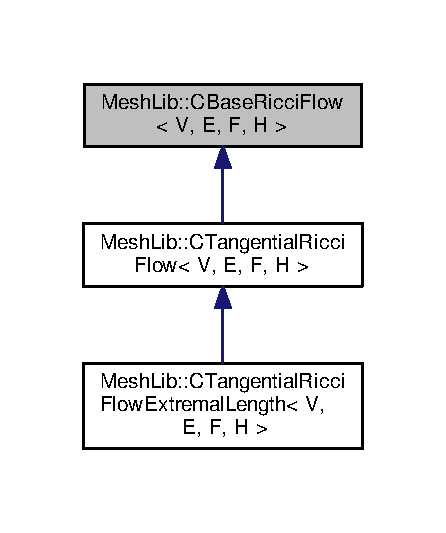
\includegraphics[width=214pt]{class_mesh_lib_1_1_c_base_ricci_flow__inherit__graph}
\end{center}
\end{figure}


Collaboration diagram for Mesh\+Lib\+:\+:C\+Base\+Ricci\+Flow$<$ V, E, F, H $>$\+:
\nopagebreak
\begin{figure}[H]
\begin{center}
\leavevmode
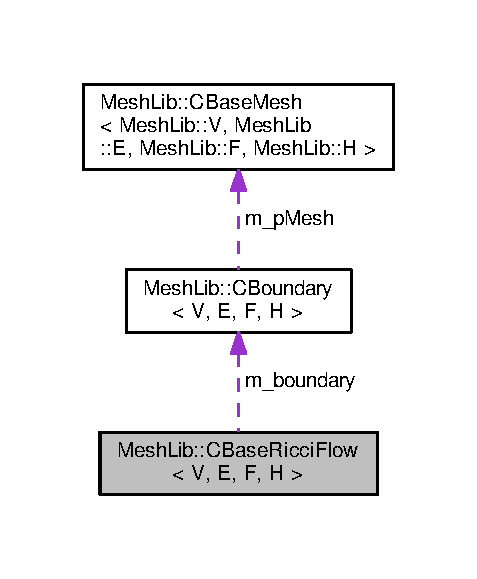
\includegraphics[width=229pt]{class_mesh_lib_1_1_c_base_ricci_flow__coll__graph}
\end{center}
\end{figure}
\subsection*{Public Member Functions}
\begin{DoxyCompactItemize}
\item 
\hyperlink{class_mesh_lib_1_1_c_base_ricci_flow_a878d8e94d5d4b83db4ee2a98021588b8}{C\+Base\+Ricci\+Flow} (C\+Ricci\+Flow\+Mesh$<$ V, E, F, H $>$ $\ast$p\+Mesh)
\begin{DoxyCompactList}\small\item\em \hyperlink{class_mesh_lib_1_1_c_base_ricci_flow}{C\+Base\+Ricci\+Flow} constructor. \end{DoxyCompactList}\item 
\hyperlink{class_mesh_lib_1_1_c_base_ricci_flow_a1b714014282163959204adfdec041eae}{$\sim$\+C\+Base\+Ricci\+Flow} ()
\begin{DoxyCompactList}\small\item\em \hyperlink{class_mesh_lib_1_1_c_base_ricci_flow}{C\+Base\+Ricci\+Flow} destructor. \end{DoxyCompactList}\item 
virtual void \hyperlink{class_mesh_lib_1_1_c_base_ricci_flow_a5e43b277b368f38f12c77e6daa9c5cd9}{\+\_\+calculate\+\_\+metric} ()
\end{DoxyCompactItemize}
\subsection*{Protected Member Functions}
\begin{DoxyCompactItemize}
\item 
virtual void \hyperlink{class_mesh_lib_1_1_c_base_ricci_flow_a58804aa74a20e99405feaf6f03f0286f}{\+\_\+length} (double u1, double u2, E $\ast$e)=0
\item 
void \hyperlink{class_mesh_lib_1_1_c_base_ricci_flow_a689bcf5fa1c50880d9073423de566228}{\+\_\+calculate\+\_\+edge\+\_\+length} ()
\item 
virtual double \hyperlink{class_mesh_lib_1_1_c_base_ricci_flow_a56a24ad8c35c165acfdd1adfac92bf25}{\+\_\+cosine\+\_\+law} (double a, double b, double c)=0
\item 
void \hyperlink{class_mesh_lib_1_1_c_base_ricci_flow_a9e8eee26f716ff1eb365abbb8091c61e}{\+\_\+calculate\+\_\+corner\+\_\+angle} ()
\item 
void \hyperlink{class_mesh_lib_1_1_c_base_ricci_flow_aff0772727106e45bc2854ffb51a4902f}{\+\_\+calculate\+\_\+vertex\+\_\+curvature} ()
\item 
double \hyperlink{class_mesh_lib_1_1_c_base_ricci_flow_adad5006c071e951e3f32f4fa6db0db83}{\+\_\+calculate\+\_\+curvature\+\_\+error} ()
\item 
virtual void \hyperlink{class_mesh_lib_1_1_c_base_ricci_flow_abf7685f1b3692a870aea756c4fdfea5c}{\+\_\+calculate\+\_\+edge\+\_\+weight} ()=0
\item 
virtual void \hyperlink{class_mesh_lib_1_1_c_base_ricci_flow_a0c8e62c086e434c38820ceec5592884e}{\+\_\+set\+\_\+target\+\_\+curvature} ()=0
\item 
virtual bool \hyperlink{class_mesh_lib_1_1_c_base_ricci_flow_a760254c91a9b18a7075ace49e6f85ba0}{\+\_\+flow} (double)
\item 
virtual void \hyperlink{class_mesh_lib_1_1_c_base_ricci_flow_ad2ecc7d640197c1ee7d4000f79ce63f8}{\+\_\+\+Newton} (double threshold, double step\+\_\+length)
\item 
virtual void \hyperlink{class_mesh_lib_1_1_c_base_ricci_flow_a65f2670e9693a0afc64d8edd5b1fd90a}{\+\_\+normalization} (Eigen\+::\+Vector\+Xd \&du, int n)=0
\item 
virtual void \hyperlink{class_mesh_lib_1_1_c_base_ricci_flow_af3f5db69f38d5085ccae21929365dda1}{\+\_\+calculate\+\_\+\+Hessain} (Eigen\+::\+Sparse\+Matrix$<$ double $>$ \&p\+Matrix)
\end{DoxyCompactItemize}
\subsection*{Protected Attributes}
\begin{DoxyCompactItemize}
\item 
C\+Ricci\+Flow\+Mesh$<$ V, E, F, H $>$ $\ast$ \hyperlink{class_mesh_lib_1_1_c_base_ricci_flow_aad696c079fc6378167052229fcfc2d5c}{m\+\_\+p\+Mesh}
\item 
\hyperlink{class_mesh_lib_1_1_c_boundary}{C\+Boundary}$<$ V, E, F, H $>$ \hyperlink{class_mesh_lib_1_1_c_base_ricci_flow_a97277c8174b4dd7ab5dfa0f369aaea42}{m\+\_\+boundary}
\end{DoxyCompactItemize}


\subsection{Detailed Description}
\subsubsection*{template$<$class V, class E, class F, class H$>$\\*
class Mesh\+Lib\+::\+C\+Base\+Ricci\+Flow$<$ V, E, F, H $>$}

Base\+Class \hyperlink{class_mesh_lib_1_1_c_base_ricci_flow}{C\+Base\+Ricci\+Flow}. 

Algorithm for computing general Ricci flow 

Definition at line 38 of file Base\+Ricci\+Flow.\+h.



\subsection{Constructor \& Destructor Documentation}
\index{Mesh\+Lib\+::\+C\+Base\+Ricci\+Flow@{Mesh\+Lib\+::\+C\+Base\+Ricci\+Flow}!C\+Base\+Ricci\+Flow@{C\+Base\+Ricci\+Flow}}
\index{C\+Base\+Ricci\+Flow@{C\+Base\+Ricci\+Flow}!Mesh\+Lib\+::\+C\+Base\+Ricci\+Flow@{Mesh\+Lib\+::\+C\+Base\+Ricci\+Flow}}
\subsubsection[{\texorpdfstring{C\+Base\+Ricci\+Flow(\+C\+Ricci\+Flow\+Mesh$<$ V, E, F, H $>$ $\ast$p\+Mesh)}{CBaseRicciFlow(CRicciFlowMesh< V, E, F, H > *pMesh)}}]{\setlength{\rightskip}{0pt plus 5cm}template$<$class V , class E , class F , class H $>$ {\bf Mesh\+Lib\+::\+C\+Base\+Ricci\+Flow}$<$ V, E, F, H $>$\+::{\bf C\+Base\+Ricci\+Flow} (
\begin{DoxyParamCaption}
\item[{C\+Ricci\+Flow\+Mesh$<$ V, E, F, H $>$ $\ast$}]{p\+Mesh}
\end{DoxyParamCaption}
)}\hypertarget{class_mesh_lib_1_1_c_base_ricci_flow_a878d8e94d5d4b83db4ee2a98021588b8}{}\label{class_mesh_lib_1_1_c_base_ricci_flow_a878d8e94d5d4b83db4ee2a98021588b8}


\hyperlink{class_mesh_lib_1_1_c_base_ricci_flow}{C\+Base\+Ricci\+Flow} constructor. 


\begin{DoxyParams}{Parameters}
{\em p\+Mesh} & the input mesh \\
\hline
\end{DoxyParams}


Definition at line 125 of file Base\+Ricci\+Flow.\+h.

\index{Mesh\+Lib\+::\+C\+Base\+Ricci\+Flow@{Mesh\+Lib\+::\+C\+Base\+Ricci\+Flow}!````~C\+Base\+Ricci\+Flow@{$\sim$\+C\+Base\+Ricci\+Flow}}
\index{````~C\+Base\+Ricci\+Flow@{$\sim$\+C\+Base\+Ricci\+Flow}!Mesh\+Lib\+::\+C\+Base\+Ricci\+Flow@{Mesh\+Lib\+::\+C\+Base\+Ricci\+Flow}}
\subsubsection[{\texorpdfstring{$\sim$\+C\+Base\+Ricci\+Flow()}{~CBaseRicciFlow()}}]{\setlength{\rightskip}{0pt plus 5cm}template$<$class V , class E , class F , class H $>$ {\bf Mesh\+Lib\+::\+C\+Base\+Ricci\+Flow}$<$ V, E, F, H $>$\+::$\sim${\bf C\+Base\+Ricci\+Flow} (
\begin{DoxyParamCaption}
{}
\end{DoxyParamCaption}
)}\hypertarget{class_mesh_lib_1_1_c_base_ricci_flow_a1b714014282163959204adfdec041eae}{}\label{class_mesh_lib_1_1_c_base_ricci_flow_a1b714014282163959204adfdec041eae}


\hyperlink{class_mesh_lib_1_1_c_base_ricci_flow}{C\+Base\+Ricci\+Flow} destructor. 



Definition at line 139 of file Base\+Ricci\+Flow.\+h.



\subsection{Member Function Documentation}
\index{Mesh\+Lib\+::\+C\+Base\+Ricci\+Flow@{Mesh\+Lib\+::\+C\+Base\+Ricci\+Flow}!\+\_\+calculate\+\_\+corner\+\_\+angle@{\+\_\+calculate\+\_\+corner\+\_\+angle}}
\index{\+\_\+calculate\+\_\+corner\+\_\+angle@{\+\_\+calculate\+\_\+corner\+\_\+angle}!Mesh\+Lib\+::\+C\+Base\+Ricci\+Flow@{Mesh\+Lib\+::\+C\+Base\+Ricci\+Flow}}
\subsubsection[{\texorpdfstring{\+\_\+calculate\+\_\+corner\+\_\+angle()}{_calculate_corner_angle()}}]{\setlength{\rightskip}{0pt plus 5cm}template$<$class V , class E , class F , class H $>$ void {\bf Mesh\+Lib\+::\+C\+Base\+Ricci\+Flow}$<$ V, E, F, H $>$\+::\+\_\+calculate\+\_\+corner\+\_\+angle (
\begin{DoxyParamCaption}
{}
\end{DoxyParamCaption}
)\hspace{0.3cm}{\ttfamily [protected]}}\hypertarget{class_mesh_lib_1_1_c_base_ricci_flow_a9e8eee26f716ff1eb365abbb8091c61e}{}\label{class_mesh_lib_1_1_c_base_ricci_flow_a9e8eee26f716ff1eb365abbb8091c61e}
Calculate corner angle 

Definition at line 168 of file Base\+Ricci\+Flow.\+h.

\index{Mesh\+Lib\+::\+C\+Base\+Ricci\+Flow@{Mesh\+Lib\+::\+C\+Base\+Ricci\+Flow}!\+\_\+calculate\+\_\+curvature\+\_\+error@{\+\_\+calculate\+\_\+curvature\+\_\+error}}
\index{\+\_\+calculate\+\_\+curvature\+\_\+error@{\+\_\+calculate\+\_\+curvature\+\_\+error}!Mesh\+Lib\+::\+C\+Base\+Ricci\+Flow@{Mesh\+Lib\+::\+C\+Base\+Ricci\+Flow}}
\subsubsection[{\texorpdfstring{\+\_\+calculate\+\_\+curvature\+\_\+error()}{_calculate_curvature_error()}}]{\setlength{\rightskip}{0pt plus 5cm}template$<$class V , class E , class F , class H $>$ double {\bf Mesh\+Lib\+::\+C\+Base\+Ricci\+Flow}$<$ V, E, F, H $>$\+::\+\_\+calculate\+\_\+curvature\+\_\+error (
\begin{DoxyParamCaption}
{}
\end{DoxyParamCaption}
)\hspace{0.3cm}{\ttfamily [protected]}}\hypertarget{class_mesh_lib_1_1_c_base_ricci_flow_adad5006c071e951e3f32f4fa6db0db83}{}\label{class_mesh_lib_1_1_c_base_ricci_flow_adad5006c071e951e3f32f4fa6db0db83}
Calculate vertex curvature error 

Definition at line 226 of file Base\+Ricci\+Flow.\+h.

\index{Mesh\+Lib\+::\+C\+Base\+Ricci\+Flow@{Mesh\+Lib\+::\+C\+Base\+Ricci\+Flow}!\+\_\+calculate\+\_\+edge\+\_\+length@{\+\_\+calculate\+\_\+edge\+\_\+length}}
\index{\+\_\+calculate\+\_\+edge\+\_\+length@{\+\_\+calculate\+\_\+edge\+\_\+length}!Mesh\+Lib\+::\+C\+Base\+Ricci\+Flow@{Mesh\+Lib\+::\+C\+Base\+Ricci\+Flow}}
\subsubsection[{\texorpdfstring{\+\_\+calculate\+\_\+edge\+\_\+length()}{_calculate_edge_length()}}]{\setlength{\rightskip}{0pt plus 5cm}template$<$class V , class E , class F , class H $>$ void {\bf Mesh\+Lib\+::\+C\+Base\+Ricci\+Flow}$<$ V, E, F, H $>$\+::\+\_\+calculate\+\_\+edge\+\_\+length (
\begin{DoxyParamCaption}
{}
\end{DoxyParamCaption}
)\hspace{0.3cm}{\ttfamily [protected]}}\hypertarget{class_mesh_lib_1_1_c_base_ricci_flow_a689bcf5fa1c50880d9073423de566228}{}\label{class_mesh_lib_1_1_c_base_ricci_flow_a689bcf5fa1c50880d9073423de566228}
Calculate each edge length 

Definition at line 146 of file Base\+Ricci\+Flow.\+h.

\index{Mesh\+Lib\+::\+C\+Base\+Ricci\+Flow@{Mesh\+Lib\+::\+C\+Base\+Ricci\+Flow}!\+\_\+calculate\+\_\+edge\+\_\+weight@{\+\_\+calculate\+\_\+edge\+\_\+weight}}
\index{\+\_\+calculate\+\_\+edge\+\_\+weight@{\+\_\+calculate\+\_\+edge\+\_\+weight}!Mesh\+Lib\+::\+C\+Base\+Ricci\+Flow@{Mesh\+Lib\+::\+C\+Base\+Ricci\+Flow}}
\subsubsection[{\texorpdfstring{\+\_\+calculate\+\_\+edge\+\_\+weight()=0}{_calculate_edge_weight()=0}}]{\setlength{\rightskip}{0pt plus 5cm}template$<$class V , class E , class F , class H $>$ virtual void {\bf Mesh\+Lib\+::\+C\+Base\+Ricci\+Flow}$<$ V, E, F, H $>$\+::\+\_\+calculate\+\_\+edge\+\_\+weight (
\begin{DoxyParamCaption}
{}
\end{DoxyParamCaption}
)\hspace{0.3cm}{\ttfamily [protected]}, {\ttfamily [pure virtual]}}\hypertarget{class_mesh_lib_1_1_c_base_ricci_flow_abf7685f1b3692a870aea756c4fdfea5c}{}\label{class_mesh_lib_1_1_c_base_ricci_flow_abf7685f1b3692a870aea756c4fdfea5c}
Calculate the edge weight 

Implemented in \hyperlink{class_mesh_lib_1_1_c_tangential_ricci_flow_a94dde69c540846106ee0daa7d840e9cb}{Mesh\+Lib\+::\+C\+Tangential\+Ricci\+Flow$<$ V, E, F, H $>$}.

\index{Mesh\+Lib\+::\+C\+Base\+Ricci\+Flow@{Mesh\+Lib\+::\+C\+Base\+Ricci\+Flow}!\+\_\+calculate\+\_\+\+Hessain@{\+\_\+calculate\+\_\+\+Hessain}}
\index{\+\_\+calculate\+\_\+\+Hessain@{\+\_\+calculate\+\_\+\+Hessain}!Mesh\+Lib\+::\+C\+Base\+Ricci\+Flow@{Mesh\+Lib\+::\+C\+Base\+Ricci\+Flow}}
\subsubsection[{\texorpdfstring{\+\_\+calculate\+\_\+\+Hessain(\+Eigen\+::\+Sparse\+Matrix$<$ double $>$ \&p\+Matrix)}{_calculate_Hessain(Eigen::SparseMatrix< double > &pMatrix)}}]{\setlength{\rightskip}{0pt plus 5cm}template$<$class V , class E , class F , class H $>$ void {\bf Mesh\+Lib\+::\+C\+Base\+Ricci\+Flow}$<$ V, E, F, H $>$\+::\+\_\+calculate\+\_\+\+Hessain (
\begin{DoxyParamCaption}
\item[{Eigen\+::\+Sparse\+Matrix$<$ double $>$ \&}]{p\+Matrix}
\end{DoxyParamCaption}
)\hspace{0.3cm}{\ttfamily [protected]}, {\ttfamily [virtual]}}\hypertarget{class_mesh_lib_1_1_c_base_ricci_flow_af3f5db69f38d5085ccae21929365dda1}{}\label{class_mesh_lib_1_1_c_base_ricci_flow_af3f5db69f38d5085ccae21929365dda1}
calculate hessian matrix Hessain 
\begin{DoxyParams}{Parameters}
{\em Sparse\+Matrix} & \\
\hline
\end{DoxyParams}


Definition at line 369 of file Base\+Ricci\+Flow.\+h.

\index{Mesh\+Lib\+::\+C\+Base\+Ricci\+Flow@{Mesh\+Lib\+::\+C\+Base\+Ricci\+Flow}!\+\_\+calculate\+\_\+metric@{\+\_\+calculate\+\_\+metric}}
\index{\+\_\+calculate\+\_\+metric@{\+\_\+calculate\+\_\+metric}!Mesh\+Lib\+::\+C\+Base\+Ricci\+Flow@{Mesh\+Lib\+::\+C\+Base\+Ricci\+Flow}}
\subsubsection[{\texorpdfstring{\+\_\+calculate\+\_\+metric()}{_calculate_metric()}}]{\setlength{\rightskip}{0pt plus 5cm}template$<$class V , class E , class F , class H $>$ void {\bf Mesh\+Lib\+::\+C\+Base\+Ricci\+Flow}$<$ V, E, F, H $>$\+::\+\_\+calculate\+\_\+metric (
\begin{DoxyParamCaption}
{}
\end{DoxyParamCaption}
)\hspace{0.3cm}{\ttfamily [virtual]}}\hypertarget{class_mesh_lib_1_1_c_base_ricci_flow_a5e43b277b368f38f12c77e6daa9c5cd9}{}\label{class_mesh_lib_1_1_c_base_ricci_flow_a5e43b277b368f38f12c77e6daa9c5cd9}
Computing the metric 

Reimplemented in \hyperlink{class_mesh_lib_1_1_c_tangential_ricci_flow_a14983a8b8819f1b37a88bed0db5d1e4a}{Mesh\+Lib\+::\+C\+Tangential\+Ricci\+Flow$<$ V, E, F, H $>$}.



Definition at line 250 of file Base\+Ricci\+Flow.\+h.

\index{Mesh\+Lib\+::\+C\+Base\+Ricci\+Flow@{Mesh\+Lib\+::\+C\+Base\+Ricci\+Flow}!\+\_\+calculate\+\_\+vertex\+\_\+curvature@{\+\_\+calculate\+\_\+vertex\+\_\+curvature}}
\index{\+\_\+calculate\+\_\+vertex\+\_\+curvature@{\+\_\+calculate\+\_\+vertex\+\_\+curvature}!Mesh\+Lib\+::\+C\+Base\+Ricci\+Flow@{Mesh\+Lib\+::\+C\+Base\+Ricci\+Flow}}
\subsubsection[{\texorpdfstring{\+\_\+calculate\+\_\+vertex\+\_\+curvature()}{_calculate_vertex_curvature()}}]{\setlength{\rightskip}{0pt plus 5cm}template$<$class V , class E , class F , class H $>$ void {\bf Mesh\+Lib\+::\+C\+Base\+Ricci\+Flow}$<$ V, E, F, H $>$\+::\+\_\+calculate\+\_\+vertex\+\_\+curvature (
\begin{DoxyParamCaption}
{}
\end{DoxyParamCaption}
)\hspace{0.3cm}{\ttfamily [protected]}}\hypertarget{class_mesh_lib_1_1_c_base_ricci_flow_aff0772727106e45bc2854ffb51a4902f}{}\label{class_mesh_lib_1_1_c_base_ricci_flow_aff0772727106e45bc2854ffb51a4902f}
Calculate vertex curvature 

Definition at line 204 of file Base\+Ricci\+Flow.\+h.

\index{Mesh\+Lib\+::\+C\+Base\+Ricci\+Flow@{Mesh\+Lib\+::\+C\+Base\+Ricci\+Flow}!\+\_\+cosine\+\_\+law@{\+\_\+cosine\+\_\+law}}
\index{\+\_\+cosine\+\_\+law@{\+\_\+cosine\+\_\+law}!Mesh\+Lib\+::\+C\+Base\+Ricci\+Flow@{Mesh\+Lib\+::\+C\+Base\+Ricci\+Flow}}
\subsubsection[{\texorpdfstring{\+\_\+cosine\+\_\+law(double a, double b, double c)=0}{_cosine_law(double a, double b, double c)=0}}]{\setlength{\rightskip}{0pt plus 5cm}template$<$class V , class E , class F , class H $>$ virtual double {\bf Mesh\+Lib\+::\+C\+Base\+Ricci\+Flow}$<$ V, E, F, H $>$\+::\+\_\+cosine\+\_\+law (
\begin{DoxyParamCaption}
\item[{double}]{a, }
\item[{double}]{b, }
\item[{double}]{c}
\end{DoxyParamCaption}
)\hspace{0.3cm}{\ttfamily [protected]}, {\ttfamily [pure virtual]}}\hypertarget{class_mesh_lib_1_1_c_base_ricci_flow_a56a24ad8c35c165acfdd1adfac92bf25}{}\label{class_mesh_lib_1_1_c_base_ricci_flow_a56a24ad8c35c165acfdd1adfac92bf25}
Cosine law, has to be defined in the derivated classes 

Implemented in \hyperlink{class_mesh_lib_1_1_c_tangential_ricci_flow_a5e066ca345120f963a6b859fbb0ac5d8}{Mesh\+Lib\+::\+C\+Tangential\+Ricci\+Flow$<$ V, E, F, H $>$}.

\index{Mesh\+Lib\+::\+C\+Base\+Ricci\+Flow@{Mesh\+Lib\+::\+C\+Base\+Ricci\+Flow}!\+\_\+flow@{\+\_\+flow}}
\index{\+\_\+flow@{\+\_\+flow}!Mesh\+Lib\+::\+C\+Base\+Ricci\+Flow@{Mesh\+Lib\+::\+C\+Base\+Ricci\+Flow}}
\subsubsection[{\texorpdfstring{\+\_\+flow(double)}{_flow(double)}}]{\setlength{\rightskip}{0pt plus 5cm}template$<$class V , class E , class F , class H $>$ bool {\bf Mesh\+Lib\+::\+C\+Base\+Ricci\+Flow}$<$ V, E, F, H $>$\+::\+\_\+flow (
\begin{DoxyParamCaption}
\item[{double}]{error\+\_\+threshold}
\end{DoxyParamCaption}
)\hspace{0.3cm}{\ttfamily [protected]}, {\ttfamily [virtual]}}\hypertarget{class_mesh_lib_1_1_c_base_ricci_flow_a760254c91a9b18a7075ace49e6f85ba0}{}\label{class_mesh_lib_1_1_c_base_ricci_flow_a760254c91a9b18a7075ace49e6f85ba0}
Curvature flow 

Reimplemented in \hyperlink{class_mesh_lib_1_1_c_tangential_ricci_flow_a5ab0113d3d85597f6a782d8ca972bad7}{Mesh\+Lib\+::\+C\+Tangential\+Ricci\+Flow$<$ V, E, F, H $>$}.



Definition at line 265 of file Base\+Ricci\+Flow.\+h.

\index{Mesh\+Lib\+::\+C\+Base\+Ricci\+Flow@{Mesh\+Lib\+::\+C\+Base\+Ricci\+Flow}!\+\_\+length@{\+\_\+length}}
\index{\+\_\+length@{\+\_\+length}!Mesh\+Lib\+::\+C\+Base\+Ricci\+Flow@{Mesh\+Lib\+::\+C\+Base\+Ricci\+Flow}}
\subsubsection[{\texorpdfstring{\+\_\+length(double u1, double u2, E $\ast$e)=0}{_length(double u1, double u2, E *e)=0}}]{\setlength{\rightskip}{0pt plus 5cm}template$<$class V , class E , class F , class H $>$ virtual void {\bf Mesh\+Lib\+::\+C\+Base\+Ricci\+Flow}$<$ V, E, F, H $>$\+::\+\_\+length (
\begin{DoxyParamCaption}
\item[{double}]{u1, }
\item[{double}]{u2, }
\item[{E $\ast$}]{e}
\end{DoxyParamCaption}
)\hspace{0.3cm}{\ttfamily [protected]}, {\ttfamily [pure virtual]}}\hypertarget{class_mesh_lib_1_1_c_base_ricci_flow_a58804aa74a20e99405feaf6f03f0286f}{}\label{class_mesh_lib_1_1_c_base_ricci_flow_a58804aa74a20e99405feaf6f03f0286f}
Calculate each edge length, has to be defined in the derivated classes 

Implemented in \hyperlink{class_mesh_lib_1_1_c_tangential_ricci_flow_a902998c914ca63c77985daeda0a1cddd}{Mesh\+Lib\+::\+C\+Tangential\+Ricci\+Flow$<$ V, E, F, H $>$}.

\index{Mesh\+Lib\+::\+C\+Base\+Ricci\+Flow@{Mesh\+Lib\+::\+C\+Base\+Ricci\+Flow}!\+\_\+\+Newton@{\+\_\+\+Newton}}
\index{\+\_\+\+Newton@{\+\_\+\+Newton}!Mesh\+Lib\+::\+C\+Base\+Ricci\+Flow@{Mesh\+Lib\+::\+C\+Base\+Ricci\+Flow}}
\subsubsection[{\texorpdfstring{\+\_\+\+Newton(double threshold, double step\+\_\+length)}{_Newton(double threshold, double step_length)}}]{\setlength{\rightskip}{0pt plus 5cm}template$<$class V , class E , class F , class H $>$ void {\bf Mesh\+Lib\+::\+C\+Base\+Ricci\+Flow}$<$ V, E, F, H $>$\+::\+\_\+\+Newton (
\begin{DoxyParamCaption}
\item[{double}]{threshold, }
\item[{double}]{step\+\_\+length}
\end{DoxyParamCaption}
)\hspace{0.3cm}{\ttfamily [protected]}, {\ttfamily [virtual]}}\hypertarget{class_mesh_lib_1_1_c_base_ricci_flow_ad2ecc7d640197c1ee7d4000f79ce63f8}{}\label{class_mesh_lib_1_1_c_base_ricci_flow_ad2ecc7d640197c1ee7d4000f79ce63f8}
Newton\textquotesingle{}s method to optimize the entropy energy 
\begin{DoxyParams}{Parameters}
{\em threshold} & err bound \\
\hline
{\em step\+\_\+length} & step length \\
\hline
\end{DoxyParams}


Definition at line 299 of file Base\+Ricci\+Flow.\+h.

\index{Mesh\+Lib\+::\+C\+Base\+Ricci\+Flow@{Mesh\+Lib\+::\+C\+Base\+Ricci\+Flow}!\+\_\+normalization@{\+\_\+normalization}}
\index{\+\_\+normalization@{\+\_\+normalization}!Mesh\+Lib\+::\+C\+Base\+Ricci\+Flow@{Mesh\+Lib\+::\+C\+Base\+Ricci\+Flow}}
\subsubsection[{\texorpdfstring{\+\_\+normalization(\+Eigen\+::\+Vector\+Xd \&du, int n)=0}{_normalization(Eigen::VectorXd &du, int n)=0}}]{\setlength{\rightskip}{0pt plus 5cm}template$<$class V , class E , class F , class H $>$ virtual void {\bf Mesh\+Lib\+::\+C\+Base\+Ricci\+Flow}$<$ V, E, F, H $>$\+::\+\_\+normalization (
\begin{DoxyParamCaption}
\item[{Eigen\+::\+Vector\+Xd \&}]{du, }
\item[{int}]{n}
\end{DoxyParamCaption}
)\hspace{0.3cm}{\ttfamily [protected]}, {\ttfamily [pure virtual]}}\hypertarget{class_mesh_lib_1_1_c_base_ricci_flow_a65f2670e9693a0afc64d8edd5b1fd90a}{}\label{class_mesh_lib_1_1_c_base_ricci_flow_a65f2670e9693a0afc64d8edd5b1fd90a}
Normalization 
\begin{DoxyParams}{Parameters}
{\em du} & the du vector \\
\hline
{\em n} & dimension of the du vector \\
\hline
\end{DoxyParams}


Implemented in \hyperlink{class_mesh_lib_1_1_c_tangential_ricci_flow_a99223f86b1f13d3974c54ce319c212fe}{Mesh\+Lib\+::\+C\+Tangential\+Ricci\+Flow$<$ V, E, F, H $>$}.

\index{Mesh\+Lib\+::\+C\+Base\+Ricci\+Flow@{Mesh\+Lib\+::\+C\+Base\+Ricci\+Flow}!\+\_\+set\+\_\+target\+\_\+curvature@{\+\_\+set\+\_\+target\+\_\+curvature}}
\index{\+\_\+set\+\_\+target\+\_\+curvature@{\+\_\+set\+\_\+target\+\_\+curvature}!Mesh\+Lib\+::\+C\+Base\+Ricci\+Flow@{Mesh\+Lib\+::\+C\+Base\+Ricci\+Flow}}
\subsubsection[{\texorpdfstring{\+\_\+set\+\_\+target\+\_\+curvature()=0}{_set_target_curvature()=0}}]{\setlength{\rightskip}{0pt plus 5cm}template$<$class V , class E , class F , class H $>$ virtual void {\bf Mesh\+Lib\+::\+C\+Base\+Ricci\+Flow}$<$ V, E, F, H $>$\+::\+\_\+set\+\_\+target\+\_\+curvature (
\begin{DoxyParamCaption}
{}
\end{DoxyParamCaption}
)\hspace{0.3cm}{\ttfamily [protected]}, {\ttfamily [pure virtual]}}\hypertarget{class_mesh_lib_1_1_c_base_ricci_flow_a0c8e62c086e434c38820ceec5592884e}{}\label{class_mesh_lib_1_1_c_base_ricci_flow_a0c8e62c086e434c38820ceec5592884e}
Set the target curvature on each vertex 

Implemented in \hyperlink{class_mesh_lib_1_1_c_tangential_ricci_flow_ab7cbb76f7ca0de62311bc9c0cfc281e5}{Mesh\+Lib\+::\+C\+Tangential\+Ricci\+Flow$<$ V, E, F, H $>$}, and \hyperlink{class_mesh_lib_1_1_c_tangential_ricci_flow_extremal_length_a2a1ba73cdc13bd1778ecbf89d632f691}{Mesh\+Lib\+::\+C\+Tangential\+Ricci\+Flow\+Extremal\+Length$<$ V, E, F, H $>$}.



\subsection{Member Data Documentation}
\index{Mesh\+Lib\+::\+C\+Base\+Ricci\+Flow@{Mesh\+Lib\+::\+C\+Base\+Ricci\+Flow}!m\+\_\+boundary@{m\+\_\+boundary}}
\index{m\+\_\+boundary@{m\+\_\+boundary}!Mesh\+Lib\+::\+C\+Base\+Ricci\+Flow@{Mesh\+Lib\+::\+C\+Base\+Ricci\+Flow}}
\subsubsection[{\texorpdfstring{m\+\_\+boundary}{m_boundary}}]{\setlength{\rightskip}{0pt plus 5cm}template$<$class V , class E , class F , class H $>$ {\bf C\+Boundary}$<$V,E,F,H$>$ {\bf Mesh\+Lib\+::\+C\+Base\+Ricci\+Flow}$<$ V, E, F, H $>$\+::m\+\_\+boundary\hspace{0.3cm}{\ttfamily [protected]}}\hypertarget{class_mesh_lib_1_1_c_base_ricci_flow_a97277c8174b4dd7ab5dfa0f369aaea42}{}\label{class_mesh_lib_1_1_c_base_ricci_flow_a97277c8174b4dd7ab5dfa0f369aaea42}
boundary of the input mesh 

Definition at line 61 of file Base\+Ricci\+Flow.\+h.

\index{Mesh\+Lib\+::\+C\+Base\+Ricci\+Flow@{Mesh\+Lib\+::\+C\+Base\+Ricci\+Flow}!m\+\_\+p\+Mesh@{m\+\_\+p\+Mesh}}
\index{m\+\_\+p\+Mesh@{m\+\_\+p\+Mesh}!Mesh\+Lib\+::\+C\+Base\+Ricci\+Flow@{Mesh\+Lib\+::\+C\+Base\+Ricci\+Flow}}
\subsubsection[{\texorpdfstring{m\+\_\+p\+Mesh}{m_pMesh}}]{\setlength{\rightskip}{0pt plus 5cm}template$<$class V , class E , class F , class H $>$ C\+Ricci\+Flow\+Mesh$<$V,E,F,H$>$$\ast$ {\bf Mesh\+Lib\+::\+C\+Base\+Ricci\+Flow}$<$ V, E, F, H $>$\+::m\+\_\+p\+Mesh\hspace{0.3cm}{\ttfamily [protected]}}\hypertarget{class_mesh_lib_1_1_c_base_ricci_flow_aad696c079fc6378167052229fcfc2d5c}{}\label{class_mesh_lib_1_1_c_base_ricci_flow_aad696c079fc6378167052229fcfc2d5c}
the input mesh 

Definition at line 57 of file Base\+Ricci\+Flow.\+h.



The documentation for this class was generated from the following file\+:\begin{DoxyCompactItemize}
\item 
Mesh\+Lib/algorithm/\+Riemannian/\+Ricci\+Flow/\hyperlink{_base_ricci_flow_8h}{Base\+Ricci\+Flow.\+h}\end{DoxyCompactItemize}

\hypertarget{class_mesh_lib_1_1_c_boundary}{}\section{Mesh\+Lib\+:\+:C\+Boundary$<$ C\+Vertex, C\+Edge, C\+Face, C\+Half\+Edge $>$ Class Template Reference}
\label{class_mesh_lib_1_1_c_boundary}\index{Mesh\+Lib\+::\+C\+Boundary$<$ C\+Vertex, C\+Edge, C\+Face, C\+Half\+Edge $>$@{Mesh\+Lib\+::\+C\+Boundary$<$ C\+Vertex, C\+Edge, C\+Face, C\+Half\+Edge $>$}}


\hyperlink{class_mesh_lib_1_1_c_boundary}{C\+Boundary} Boundary class.  




{\ttfamily \#include $<$boundary.\+h$>$}



Collaboration diagram for Mesh\+Lib\+:\+:C\+Boundary$<$ C\+Vertex, C\+Edge, C\+Face, C\+Half\+Edge $>$\+:
\nopagebreak
\begin{figure}[H]
\begin{center}
\leavevmode
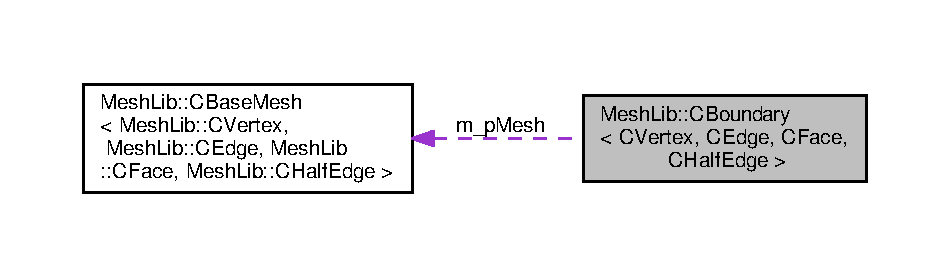
\includegraphics[width=350pt]{class_mesh_lib_1_1_c_boundary__coll__graph}
\end{center}
\end{figure}
\subsection*{Public Member Functions}
\begin{DoxyCompactItemize}
\item 
\hyperlink{class_mesh_lib_1_1_c_boundary_ae8f0ae5dcbd7083268dd22b4db773c88}{C\+Boundary} (\hyperlink{class_mesh_lib_1_1_c_base_mesh}{C\+Base\+Mesh}$<$ \hyperlink{class_mesh_lib_1_1_c_vertex}{C\+Vertex}, \hyperlink{class_mesh_lib_1_1_c_edge}{C\+Edge}, \hyperlink{class_mesh_lib_1_1_c_face}{C\+Face}, \hyperlink{class_mesh_lib_1_1_c_half_edge}{C\+Half\+Edge} $>$ $\ast$p\+Mesh)
\item 
\hyperlink{class_mesh_lib_1_1_c_boundary_ac46449d5cb6708f2da90a2314ae1e9ba}{$\sim$\+C\+Boundary} ()
\item 
std\+::vector$<$ \hyperlink{class_mesh_lib_1_1_c_loop}{T\+Loop} $\ast$ $>$ \& \hyperlink{class_mesh_lib_1_1_c_boundary_aa71cb8a6d3f8107da8dad93523da97db}{loops} ()
\end{DoxyCompactItemize}
\subsection*{Protected Member Functions}
\begin{DoxyCompactItemize}
\item 
void \hyperlink{class_mesh_lib_1_1_c_boundary_a323f8a0aa90198d55814cac0e3477228}{\+\_\+bubble\+\_\+sort} (std\+::vector$<$ \hyperlink{class_mesh_lib_1_1_c_loop}{C\+Loop}$<$ \hyperlink{class_mesh_lib_1_1_c_vertex}{C\+Vertex}, \hyperlink{class_mesh_lib_1_1_c_edge}{C\+Edge}, \hyperlink{class_mesh_lib_1_1_c_face}{C\+Face}, \hyperlink{class_mesh_lib_1_1_c_half_edge}{C\+Half\+Edge} $>$ $\ast$ $>$ \&\hyperlink{class_mesh_lib_1_1_c_boundary_aa71cb8a6d3f8107da8dad93523da97db}{loops})
\end{DoxyCompactItemize}
\subsection*{Protected Attributes}
\begin{DoxyCompactItemize}
\item 
\hyperlink{class_mesh_lib_1_1_c_base_mesh}{C\+Base\+Mesh}$<$ \hyperlink{class_mesh_lib_1_1_c_vertex}{C\+Vertex}, \hyperlink{class_mesh_lib_1_1_c_edge}{C\+Edge}, \hyperlink{class_mesh_lib_1_1_c_face}{C\+Face}, \hyperlink{class_mesh_lib_1_1_c_half_edge}{C\+Half\+Edge} $>$ $\ast$ \hyperlink{class_mesh_lib_1_1_c_boundary_aa8433a77082ef2564f6dde8abac6cccf}{m\+\_\+p\+Mesh}
\item 
std\+::vector$<$ \hyperlink{class_mesh_lib_1_1_c_loop}{T\+Loop} $\ast$ $>$ \hyperlink{class_mesh_lib_1_1_c_boundary_aace53fe51b6ce09ba0d0f59a92ef413b}{m\+\_\+loops}
\end{DoxyCompactItemize}


\subsection{Detailed Description}
\subsubsection*{template$<$class C\+Vertex, class C\+Edge, class C\+Face, class C\+Half\+Edge$>$\\*
class Mesh\+Lib\+::\+C\+Boundary$<$ C\+Vertex, C\+Edge, C\+Face, C\+Half\+Edge $>$}

\hyperlink{class_mesh_lib_1_1_c_boundary}{C\+Boundary} Boundary class. 


\begin{DoxyTemplParams}{Template Parameters}
{\em \hyperlink{class_mesh_lib_1_1_c_vertex}{C\+Vertex}} & Vertex type \\
\hline
{\em \hyperlink{class_mesh_lib_1_1_c_edge}{C\+Edge}} & Edge type \\
\hline
{\em \hyperlink{class_mesh_lib_1_1_c_face}{C\+Face}} & Face type \\
\hline
{\em \hyperlink{class_mesh_lib_1_1_c_half_edge}{C\+Half\+Edge}} & Half\+Edge type \\
\hline
\end{DoxyTemplParams}


Definition at line 107 of file boundary.\+h.



\subsection{Constructor \& Destructor Documentation}
\index{Mesh\+Lib\+::\+C\+Boundary@{Mesh\+Lib\+::\+C\+Boundary}!C\+Boundary@{C\+Boundary}}
\index{C\+Boundary@{C\+Boundary}!Mesh\+Lib\+::\+C\+Boundary@{Mesh\+Lib\+::\+C\+Boundary}}
\subsubsection[{\texorpdfstring{C\+Boundary(\+C\+Base\+Mesh$<$ C\+Vertex, C\+Edge, C\+Face, C\+Half\+Edge $>$ $\ast$p\+Mesh)}{CBoundary(CBaseMesh< CVertex, CEdge, CFace, CHalfEdge > *pMesh)}}]{\setlength{\rightskip}{0pt plus 5cm}template$<$class C\+Vertex, class C\+Edge, class C\+Face, class C\+Half\+Edge$>$ {\bf Mesh\+Lib\+::\+C\+Boundary}$<$ {\bf C\+Vertex}, {\bf C\+Edge}, {\bf C\+Face}, {\bf C\+Half\+Edge} $>$\+::{\bf C\+Boundary} (
\begin{DoxyParamCaption}
\item[{{\bf C\+Base\+Mesh}$<$ {\bf C\+Vertex}, {\bf C\+Edge}, {\bf C\+Face}, {\bf C\+Half\+Edge} $>$ $\ast$}]{p\+Mesh}
\end{DoxyParamCaption}
)}\hypertarget{class_mesh_lib_1_1_c_boundary_ae8f0ae5dcbd7083268dd22b4db773c88}{}\label{class_mesh_lib_1_1_c_boundary_ae8f0ae5dcbd7083268dd22b4db773c88}
\hyperlink{class_mesh_lib_1_1_c_boundary}{C\+Boundary} constructor 
\begin{DoxyParams}{Parameters}
{\em p\+Mesh} & pointer to the current mesh\\
\hline
\end{DoxyParams}
\hyperlink{class_mesh_lib_1_1_c_boundary}{C\+Boundary} constructor 
\begin{DoxyParams}{Parameters}
{\em p\+Mesh} & the current mesh \\
\hline
\end{DoxyParams}


Definition at line 213 of file boundary.\+h.

\index{Mesh\+Lib\+::\+C\+Boundary@{Mesh\+Lib\+::\+C\+Boundary}!````~C\+Boundary@{$\sim$\+C\+Boundary}}
\index{````~C\+Boundary@{$\sim$\+C\+Boundary}!Mesh\+Lib\+::\+C\+Boundary@{Mesh\+Lib\+::\+C\+Boundary}}
\subsubsection[{\texorpdfstring{$\sim$\+C\+Boundary()}{~CBoundary()}}]{\setlength{\rightskip}{0pt plus 5cm}template$<$class C\+Vertex , class C\+Edge , class C\+Face , class C\+Half\+Edge $>$ {\bf Mesh\+Lib\+::\+C\+Boundary}$<$ {\bf C\+Vertex}, {\bf C\+Edge}, {\bf C\+Face}, {\bf C\+Half\+Edge} $>$\+::$\sim${\bf C\+Boundary} (
\begin{DoxyParamCaption}
{}
\end{DoxyParamCaption}
)}\hypertarget{class_mesh_lib_1_1_c_boundary_ac46449d5cb6708f2da90a2314ae1e9ba}{}\label{class_mesh_lib_1_1_c_boundary_ac46449d5cb6708f2da90a2314ae1e9ba}
\hyperlink{class_mesh_lib_1_1_c_boundary}{C\+Boundary} destructor

\hyperlink{class_mesh_lib_1_1_c_boundary}{C\+Boundary} destructor, delete all boundary loop objects. 

Definition at line 255 of file boundary.\+h.



\subsection{Member Function Documentation}
\index{Mesh\+Lib\+::\+C\+Boundary@{Mesh\+Lib\+::\+C\+Boundary}!\+\_\+bubble\+\_\+sort@{\+\_\+bubble\+\_\+sort}}
\index{\+\_\+bubble\+\_\+sort@{\+\_\+bubble\+\_\+sort}!Mesh\+Lib\+::\+C\+Boundary@{Mesh\+Lib\+::\+C\+Boundary}}
\subsubsection[{\texorpdfstring{\+\_\+bubble\+\_\+sort(std\+::vector$<$ C\+Loop$<$ C\+Vertex, C\+Edge, C\+Face, C\+Half\+Edge $>$ $\ast$ $>$ \&loops)}{_bubble_sort(std::vector< CLoop< CVertex, CEdge, CFace, CHalfEdge > * > &loops)}}]{\setlength{\rightskip}{0pt plus 5cm}template$<$class C\+Vertex, class C\+Edge, class C\+Face, class C\+Half\+Edge$>$ void {\bf Mesh\+Lib\+::\+C\+Boundary}$<$ {\bf C\+Vertex}, {\bf C\+Edge}, {\bf C\+Face}, {\bf C\+Half\+Edge} $>$\+::\+\_\+bubble\+\_\+sort (
\begin{DoxyParamCaption}
\item[{std\+::vector$<$ {\bf C\+Loop}$<$ {\bf C\+Vertex}, {\bf C\+Edge}, {\bf C\+Face}, {\bf C\+Half\+Edge} $>$ $\ast$ $>$ \&}]{loops}
\end{DoxyParamCaption}
)\hspace{0.3cm}{\ttfamily [protected]}}\hypertarget{class_mesh_lib_1_1_c_boundary_a323f8a0aa90198d55814cac0e3477228}{}\label{class_mesh_lib_1_1_c_boundary_a323f8a0aa90198d55814cac0e3477228}
Bubble sort the loops 
\begin{DoxyParams}{Parameters}
{\em loops} & the vector of loops\\
\hline
\end{DoxyParams}
\+\_\+bubble\+\_\+sort bubble sort a vector of boundary loop objects, according to their lengths 
\begin{DoxyParams}{Parameters}
{\em loops} & vector of loops \\
\hline
\end{DoxyParams}


Definition at line 186 of file boundary.\+h.

\index{Mesh\+Lib\+::\+C\+Boundary@{Mesh\+Lib\+::\+C\+Boundary}!loops@{loops}}
\index{loops@{loops}!Mesh\+Lib\+::\+C\+Boundary@{Mesh\+Lib\+::\+C\+Boundary}}
\subsubsection[{\texorpdfstring{loops()}{loops()}}]{\setlength{\rightskip}{0pt plus 5cm}template$<$class C\+Vertex, class C\+Edge, class C\+Face, class C\+Half\+Edge$>$ std\+::vector$<${\bf T\+Loop}$\ast$$>$\& {\bf Mesh\+Lib\+::\+C\+Boundary}$<$ {\bf C\+Vertex}, {\bf C\+Edge}, {\bf C\+Face}, {\bf C\+Half\+Edge} $>$\+::loops (
\begin{DoxyParamCaption}
{}
\end{DoxyParamCaption}
)\hspace{0.3cm}{\ttfamily [inline]}}\hypertarget{class_mesh_lib_1_1_c_boundary_aa71cb8a6d3f8107da8dad93523da97db}{}\label{class_mesh_lib_1_1_c_boundary_aa71cb8a6d3f8107da8dad93523da97db}
The list of boundary loops. 

Definition at line 124 of file boundary.\+h.



\subsection{Member Data Documentation}
\index{Mesh\+Lib\+::\+C\+Boundary@{Mesh\+Lib\+::\+C\+Boundary}!m\+\_\+loops@{m\+\_\+loops}}
\index{m\+\_\+loops@{m\+\_\+loops}!Mesh\+Lib\+::\+C\+Boundary@{Mesh\+Lib\+::\+C\+Boundary}}
\subsubsection[{\texorpdfstring{m\+\_\+loops}{m_loops}}]{\setlength{\rightskip}{0pt plus 5cm}template$<$class C\+Vertex, class C\+Edge, class C\+Face, class C\+Half\+Edge$>$ std\+::vector$<${\bf T\+Loop}$\ast$$>$ {\bf Mesh\+Lib\+::\+C\+Boundary}$<$ {\bf C\+Vertex}, {\bf C\+Edge}, {\bf C\+Face}, {\bf C\+Half\+Edge} $>$\+::m\+\_\+loops\hspace{0.3cm}{\ttfamily [protected]}}\hypertarget{class_mesh_lib_1_1_c_boundary_aace53fe51b6ce09ba0d0f59a92ef413b}{}\label{class_mesh_lib_1_1_c_boundary_aace53fe51b6ce09ba0d0f59a92ef413b}
List of boundary loops. 

Definition at line 137 of file boundary.\+h.

\index{Mesh\+Lib\+::\+C\+Boundary@{Mesh\+Lib\+::\+C\+Boundary}!m\+\_\+p\+Mesh@{m\+\_\+p\+Mesh}}
\index{m\+\_\+p\+Mesh@{m\+\_\+p\+Mesh}!Mesh\+Lib\+::\+C\+Boundary@{Mesh\+Lib\+::\+C\+Boundary}}
\subsubsection[{\texorpdfstring{m\+\_\+p\+Mesh}{m_pMesh}}]{\setlength{\rightskip}{0pt plus 5cm}template$<$class C\+Vertex, class C\+Edge, class C\+Face, class C\+Half\+Edge$>$ {\bf C\+Base\+Mesh}$<${\bf C\+Vertex},{\bf C\+Edge},{\bf C\+Face},{\bf C\+Half\+Edge}$>$$\ast$ {\bf Mesh\+Lib\+::\+C\+Boundary}$<$ {\bf C\+Vertex}, {\bf C\+Edge}, {\bf C\+Face}, {\bf C\+Half\+Edge} $>$\+::m\+\_\+p\+Mesh\hspace{0.3cm}{\ttfamily [protected]}}\hypertarget{class_mesh_lib_1_1_c_boundary_aa8433a77082ef2564f6dde8abac6cccf}{}\label{class_mesh_lib_1_1_c_boundary_aa8433a77082ef2564f6dde8abac6cccf}
Pointer to the current mesh. 

Definition at line 133 of file boundary.\+h.



The documentation for this class was generated from the following file\+:\begin{DoxyCompactItemize}
\item 
Mesh\+Lib/core/\+Mesh/\hyperlink{boundary_8h}{boundary.\+h}\end{DoxyCompactItemize}

\hypertarget{class_mesh_lib_1_1_c_circle}{}\section{Mesh\+Lib\+:\+:C\+Circle Class Reference}
\label{class_mesh_lib_1_1_c_circle}\index{Mesh\+Lib\+::\+C\+Circle@{Mesh\+Lib\+::\+C\+Circle}}


\hyperlink{class_mesh_lib_1_1_c_circle}{C\+Circle} class, circle on the plane.  




{\ttfamily \#include $<$Circle.\+h$>$}

\subsection*{Public Member Functions}
\begin{DoxyCompactItemize}
\item 
\hyperlink{class_mesh_lib_1_1_c_circle_ac93a47d827130cb3c3cb25724f19685f}{C\+Circle} ()
\item 
\hyperlink{class_mesh_lib_1_1_c_circle_a228003f30ff009cdd5b086cc71c7527f}{C\+Circle} (const \hyperlink{class_mesh_lib_1_1_c_point2}{C\+Point2} \&\hyperlink{class_mesh_lib_1_1_c_circle_ab3fae322fad5402d3f9df36d20d3416d}{c}, const double \hyperlink{class_mesh_lib_1_1_c_circle_a0f097b93f99ce4f540bc2e0351751932}{r})
\item 
\hyperlink{class_mesh_lib_1_1_c_circle_ab5c4fca3b7a12c0c9891762ae898ece3}{$\sim$\+C\+Circle} ()
\item 
\hyperlink{class_mesh_lib_1_1_c_point2}{C\+Point2} \& \hyperlink{class_mesh_lib_1_1_c_circle_ab3fae322fad5402d3f9df36d20d3416d}{c} ()
\item 
double \& \hyperlink{class_mesh_lib_1_1_c_circle_a0f097b93f99ce4f540bc2e0351751932}{r} ()
\end{DoxyCompactItemize}


\subsection{Detailed Description}
\hyperlink{class_mesh_lib_1_1_c_circle}{C\+Circle} class, circle on the plane. 

Circle on the two dimensional plane 

Definition at line 22 of file Circle.\+h.



\subsection{Constructor \& Destructor Documentation}
\index{Mesh\+Lib\+::\+C\+Circle@{Mesh\+Lib\+::\+C\+Circle}!C\+Circle@{C\+Circle}}
\index{C\+Circle@{C\+Circle}!Mesh\+Lib\+::\+C\+Circle@{Mesh\+Lib\+::\+C\+Circle}}
\subsubsection[{\texorpdfstring{C\+Circle()}{CCircle()}}]{\setlength{\rightskip}{0pt plus 5cm}Mesh\+Lib\+::\+C\+Circle\+::\+C\+Circle (
\begin{DoxyParamCaption}
{}
\end{DoxyParamCaption}
)\hspace{0.3cm}{\ttfamily [inline]}}\hypertarget{class_mesh_lib_1_1_c_circle_ac93a47d827130cb3c3cb25724f19685f}{}\label{class_mesh_lib_1_1_c_circle_ac93a47d827130cb3c3cb25724f19685f}
\hyperlink{class_mesh_lib_1_1_c_circle}{C\+Circle} default constructor, it is initialized to be ((0,0),1) 

Definition at line 28 of file Circle.\+h.

\index{Mesh\+Lib\+::\+C\+Circle@{Mesh\+Lib\+::\+C\+Circle}!C\+Circle@{C\+Circle}}
\index{C\+Circle@{C\+Circle}!Mesh\+Lib\+::\+C\+Circle@{Mesh\+Lib\+::\+C\+Circle}}
\subsubsection[{\texorpdfstring{C\+Circle(const C\+Point2 \&c, const double r)}{CCircle(const CPoint2 &c, const double r)}}]{\setlength{\rightskip}{0pt plus 5cm}Mesh\+Lib\+::\+C\+Circle\+::\+C\+Circle (
\begin{DoxyParamCaption}
\item[{const {\bf C\+Point2} \&}]{c, }
\item[{const double}]{r}
\end{DoxyParamCaption}
)\hspace{0.3cm}{\ttfamily [inline]}}\hypertarget{class_mesh_lib_1_1_c_circle_a228003f30ff009cdd5b086cc71c7527f}{}\label{class_mesh_lib_1_1_c_circle_a228003f30ff009cdd5b086cc71c7527f}
\hyperlink{class_mesh_lib_1_1_c_circle}{C\+Circle} class copy operator 

Definition at line 32 of file Circle.\+h.

\index{Mesh\+Lib\+::\+C\+Circle@{Mesh\+Lib\+::\+C\+Circle}!````~C\+Circle@{$\sim$\+C\+Circle}}
\index{````~C\+Circle@{$\sim$\+C\+Circle}!Mesh\+Lib\+::\+C\+Circle@{Mesh\+Lib\+::\+C\+Circle}}
\subsubsection[{\texorpdfstring{$\sim$\+C\+Circle()}{~CCircle()}}]{\setlength{\rightskip}{0pt plus 5cm}Mesh\+Lib\+::\+C\+Circle\+::$\sim$\+C\+Circle (
\begin{DoxyParamCaption}
{}
\end{DoxyParamCaption}
)\hspace{0.3cm}{\ttfamily [inline]}}\hypertarget{class_mesh_lib_1_1_c_circle_ab5c4fca3b7a12c0c9891762ae898ece3}{}\label{class_mesh_lib_1_1_c_circle_ab5c4fca3b7a12c0c9891762ae898ece3}
\hyperlink{class_mesh_lib_1_1_c_circle}{C\+Circle} class destructor 

Definition at line 36 of file Circle.\+h.



\subsection{Member Function Documentation}
\index{Mesh\+Lib\+::\+C\+Circle@{Mesh\+Lib\+::\+C\+Circle}!c@{c}}
\index{c@{c}!Mesh\+Lib\+::\+C\+Circle@{Mesh\+Lib\+::\+C\+Circle}}
\subsubsection[{\texorpdfstring{c()}{c()}}]{\setlength{\rightskip}{0pt plus 5cm}{\bf C\+Point2}\& Mesh\+Lib\+::\+C\+Circle\+::c (
\begin{DoxyParamCaption}
{}
\end{DoxyParamCaption}
)\hspace{0.3cm}{\ttfamily [inline]}}\hypertarget{class_mesh_lib_1_1_c_circle_ab3fae322fad5402d3f9df36d20d3416d}{}\label{class_mesh_lib_1_1_c_circle_ab3fae322fad5402d3f9df36d20d3416d}
The center of the circle 

Definition at line 42 of file Circle.\+h.

\index{Mesh\+Lib\+::\+C\+Circle@{Mesh\+Lib\+::\+C\+Circle}!r@{r}}
\index{r@{r}!Mesh\+Lib\+::\+C\+Circle@{Mesh\+Lib\+::\+C\+Circle}}
\subsubsection[{\texorpdfstring{r()}{r()}}]{\setlength{\rightskip}{0pt plus 5cm}double\& Mesh\+Lib\+::\+C\+Circle\+::r (
\begin{DoxyParamCaption}
{}
\end{DoxyParamCaption}
)\hspace{0.3cm}{\ttfamily [inline]}}\hypertarget{class_mesh_lib_1_1_c_circle_a0f097b93f99ce4f540bc2e0351751932}{}\label{class_mesh_lib_1_1_c_circle_a0f097b93f99ce4f540bc2e0351751932}
The radius of the circle 

Definition at line 47 of file Circle.\+h.



The documentation for this class was generated from the following file\+:\begin{DoxyCompactItemize}
\item 
Mesh\+Lib/core/\+Geometry/\hyperlink{_circle_8h}{Circle.\+h}\end{DoxyCompactItemize}

\hypertarget{class_mesh_lib_1_1_c_dynamic_mesh}{}\section{Mesh\+Lib\+:\+:C\+Dynamic\+Mesh$<$ V, E, F, H $>$ Class Template Reference}
\label{class_mesh_lib_1_1_c_dynamic_mesh}\index{Mesh\+Lib\+::\+C\+Dynamic\+Mesh$<$ V, E, F, H $>$@{Mesh\+Lib\+::\+C\+Dynamic\+Mesh$<$ V, E, F, H $>$}}


\hyperlink{class_mesh_lib_1_1_c_dynamic_mesh}{C\+Dynamic\+Mesh} class \+: Dynamic mesh.  




{\ttfamily \#include $<$Dynamic\+Mesh.\+h$>$}



Inheritance diagram for Mesh\+Lib\+:\+:C\+Dynamic\+Mesh$<$ V, E, F, H $>$\+:
\nopagebreak
\begin{figure}[H]
\begin{center}
\leavevmode
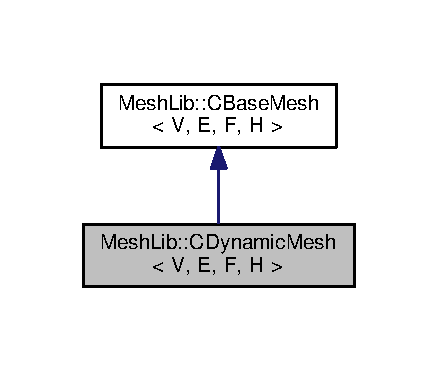
\includegraphics[width=210pt]{class_mesh_lib_1_1_c_dynamic_mesh__inherit__graph}
\end{center}
\end{figure}


Collaboration diagram for Mesh\+Lib\+:\+:C\+Dynamic\+Mesh$<$ V, E, F, H $>$\+:
\nopagebreak
\begin{figure}[H]
\begin{center}
\leavevmode
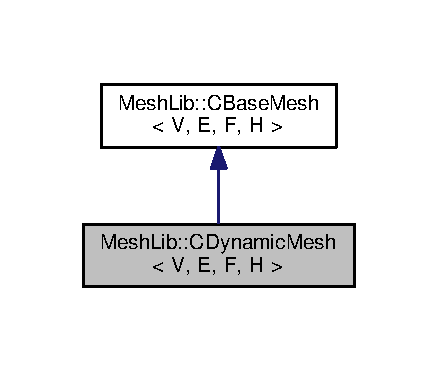
\includegraphics[width=210pt]{class_mesh_lib_1_1_c_dynamic_mesh__coll__graph}
\end{center}
\end{figure}
\subsection*{Public Member Functions}
\begin{DoxyCompactItemize}
\item 
\hyperlink{class_mesh_lib_1_1_c_dynamic_mesh_a18dd6f395ba9e07c4d8372fd0a97e6ed}{C\+Dynamic\+Mesh} ()
\item 
\hyperlink{class_mesh_lib_1_1_c_dynamic_mesh_a69bc3754b47de04cbaf986b2544593a3}{$\sim$\+C\+Dynamic\+Mesh} ()
\item 
V $\ast$ \hyperlink{class_mesh_lib_1_1_c_dynamic_mesh_a9ddf90db68fb55fe7848e881b9ecef23}{split\+Face} (F $\ast$p\+Face)
\item 
V $\ast$ \hyperlink{class_mesh_lib_1_1_c_dynamic_mesh_aa793d46c1ee19c3e40fe5c4f9b31b2e8}{split\+Edge} (E $\ast$p\+Edge)
\item 
void \hyperlink{class_mesh_lib_1_1_c_dynamic_mesh_a6a24a61f7b4bb4a48427a4149a24d630}{swap\+Edge} (E $\ast$edge)
\end{DoxyCompactItemize}
\subsection*{Protected Member Functions}
\begin{DoxyCompactItemize}
\item 
void \hyperlink{class_mesh_lib_1_1_c_dynamic_mesh_ae069e367095757cc53bf9218aad6ef06}{\+\_\+\+\_\+attach\+\_\+halfedge\+\_\+to\+\_\+edge} (H $\ast$he0, H $\ast$he1, E $\ast$e)
\end{DoxyCompactItemize}
\subsection*{Protected Attributes}
\begin{DoxyCompactItemize}
\item 
int \hyperlink{class_mesh_lib_1_1_c_dynamic_mesh_aeb1cf2cd71ab4f8845c3d5204a0ca93d}{m\+\_\+vertex\+\_\+id}
\item 
int \hyperlink{class_mesh_lib_1_1_c_dynamic_mesh_af59ef3c93fa120fba2165f43f04c80ad}{m\+\_\+face\+\_\+id}
\end{DoxyCompactItemize}
\subsection*{Additional Inherited Members}


\subsection{Detailed Description}
\subsubsection*{template$<$class V, class E, class F, class H$>$\\*
class Mesh\+Lib\+::\+C\+Dynamic\+Mesh$<$ V, E, F, H $>$}

\hyperlink{class_mesh_lib_1_1_c_dynamic_mesh}{C\+Dynamic\+Mesh} class \+: Dynamic mesh. 

Mesh supports Face\+Slit, Edge\+Slit, Edge\+Swap operations 

Definition at line 37 of file Dynamic\+Mesh.\+h.



\subsection{Constructor \& Destructor Documentation}
\index{Mesh\+Lib\+::\+C\+Dynamic\+Mesh@{Mesh\+Lib\+::\+C\+Dynamic\+Mesh}!C\+Dynamic\+Mesh@{C\+Dynamic\+Mesh}}
\index{C\+Dynamic\+Mesh@{C\+Dynamic\+Mesh}!Mesh\+Lib\+::\+C\+Dynamic\+Mesh@{Mesh\+Lib\+::\+C\+Dynamic\+Mesh}}
\subsubsection[{\texorpdfstring{C\+Dynamic\+Mesh()}{CDynamicMesh()}}]{\setlength{\rightskip}{0pt plus 5cm}template$<$class V , class E , class F , class H $>$ {\bf Mesh\+Lib\+::\+C\+Dynamic\+Mesh}$<$ V, E, F, H $>$\+::{\bf C\+Dynamic\+Mesh} (
\begin{DoxyParamCaption}
{}
\end{DoxyParamCaption}
)\hspace{0.3cm}{\ttfamily [inline]}}\hypertarget{class_mesh_lib_1_1_c_dynamic_mesh_a18dd6f395ba9e07c4d8372fd0a97e6ed}{}\label{class_mesh_lib_1_1_c_dynamic_mesh_a18dd6f395ba9e07c4d8372fd0a97e6ed}
\hyperlink{class_mesh_lib_1_1_c_dynamic_mesh}{C\+Dynamic\+Mesh} constructor 

Definition at line 41 of file Dynamic\+Mesh.\+h.

\index{Mesh\+Lib\+::\+C\+Dynamic\+Mesh@{Mesh\+Lib\+::\+C\+Dynamic\+Mesh}!````~C\+Dynamic\+Mesh@{$\sim$\+C\+Dynamic\+Mesh}}
\index{````~C\+Dynamic\+Mesh@{$\sim$\+C\+Dynamic\+Mesh}!Mesh\+Lib\+::\+C\+Dynamic\+Mesh@{Mesh\+Lib\+::\+C\+Dynamic\+Mesh}}
\subsubsection[{\texorpdfstring{$\sim$\+C\+Dynamic\+Mesh()}{~CDynamicMesh()}}]{\setlength{\rightskip}{0pt plus 5cm}template$<$class V , class E , class F , class H $>$ {\bf Mesh\+Lib\+::\+C\+Dynamic\+Mesh}$<$ V, E, F, H $>$\+::$\sim${\bf C\+Dynamic\+Mesh} (
\begin{DoxyParamCaption}
{}
\end{DoxyParamCaption}
)}\hypertarget{class_mesh_lib_1_1_c_dynamic_mesh_a69bc3754b47de04cbaf986b2544593a3}{}\label{class_mesh_lib_1_1_c_dynamic_mesh_a69bc3754b47de04cbaf986b2544593a3}
\hyperlink{class_mesh_lib_1_1_c_dynamic_mesh}{C\+Dynamic\+Mesh} destructor 

Definition at line 75 of file Dynamic\+Mesh.\+h.



\subsection{Member Function Documentation}
\index{Mesh\+Lib\+::\+C\+Dynamic\+Mesh@{Mesh\+Lib\+::\+C\+Dynamic\+Mesh}!\+\_\+\+\_\+attach\+\_\+halfedge\+\_\+to\+\_\+edge@{\+\_\+\+\_\+attach\+\_\+halfedge\+\_\+to\+\_\+edge}}
\index{\+\_\+\+\_\+attach\+\_\+halfedge\+\_\+to\+\_\+edge@{\+\_\+\+\_\+attach\+\_\+halfedge\+\_\+to\+\_\+edge}!Mesh\+Lib\+::\+C\+Dynamic\+Mesh@{Mesh\+Lib\+::\+C\+Dynamic\+Mesh}}
\subsubsection[{\texorpdfstring{\+\_\+\+\_\+attach\+\_\+halfedge\+\_\+to\+\_\+edge(\+H $\ast$he0, H $\ast$he1, E $\ast$e)}{__attach_halfedge_to_edge(H *he0, H *he1, E *e)}}]{\setlength{\rightskip}{0pt plus 5cm}template$<$class V , class E , class F , class H $>$ void {\bf Mesh\+Lib\+::\+C\+Dynamic\+Mesh}$<$ {\bf C\+Vertex}, {\bf C\+Edge}, {\bf C\+Face}, {\bf C\+Half\+Edge} $>$\+::\+\_\+\+\_\+attach\+\_\+halfedge\+\_\+to\+\_\+edge (
\begin{DoxyParamCaption}
\item[{H $\ast$}]{he0, }
\item[{H $\ast$}]{he1, }
\item[{E $\ast$}]{e}
\end{DoxyParamCaption}
)\hspace{0.3cm}{\ttfamily [protected]}}\hypertarget{class_mesh_lib_1_1_c_dynamic_mesh_ae069e367095757cc53bf9218aad6ef06}{}\label{class_mesh_lib_1_1_c_dynamic_mesh_ae069e367095757cc53bf9218aad6ef06}
attach halfeges to an edge 
\begin{DoxyParams}{Parameters}
{\em he0,he1} & the halfedges \\
\hline
{\em e} & edge \\
\hline
\end{DoxyParams}


Definition at line 473 of file Dynamic\+Mesh.\+h.

\index{Mesh\+Lib\+::\+C\+Dynamic\+Mesh@{Mesh\+Lib\+::\+C\+Dynamic\+Mesh}!split\+Edge@{split\+Edge}}
\index{split\+Edge@{split\+Edge}!Mesh\+Lib\+::\+C\+Dynamic\+Mesh@{Mesh\+Lib\+::\+C\+Dynamic\+Mesh}}
\subsubsection[{\texorpdfstring{split\+Edge(\+E $\ast$p\+Edge)}{splitEdge(E *pEdge)}}]{\setlength{\rightskip}{0pt plus 5cm}template$<$class V , class E , class F , class H $>$ {\bf C\+Vertex} $\ast$ {\bf Mesh\+Lib\+::\+C\+Dynamic\+Mesh}$<$ {\bf C\+Vertex}, {\bf C\+Edge}, {\bf C\+Face}, {\bf C\+Half\+Edge} $>$\+::split\+Edge (
\begin{DoxyParamCaption}
\item[{E $\ast$}]{p\+Edge}
\end{DoxyParamCaption}
)}\hypertarget{class_mesh_lib_1_1_c_dynamic_mesh_aa793d46c1ee19c3e40fe5c4f9b31b2e8}{}\label{class_mesh_lib_1_1_c_dynamic_mesh_aa793d46c1ee19c3e40fe5c4f9b31b2e8}
Split one edge to two edges 
\begin{DoxyParams}{Parameters}
{\em p\+Edge} & the edge to be split \\
\hline
\end{DoxyParams}


Definition at line 330 of file Dynamic\+Mesh.\+h.

\index{Mesh\+Lib\+::\+C\+Dynamic\+Mesh@{Mesh\+Lib\+::\+C\+Dynamic\+Mesh}!split\+Face@{split\+Face}}
\index{split\+Face@{split\+Face}!Mesh\+Lib\+::\+C\+Dynamic\+Mesh@{Mesh\+Lib\+::\+C\+Dynamic\+Mesh}}
\subsubsection[{\texorpdfstring{split\+Face(\+F $\ast$p\+Face)}{splitFace(F *pFace)}}]{\setlength{\rightskip}{0pt plus 5cm}template$<$class V , class E , class F , class H $>$ {\bf C\+Vertex} $\ast$ {\bf Mesh\+Lib\+::\+C\+Dynamic\+Mesh}$<$ {\bf C\+Vertex}, {\bf C\+Edge}, {\bf C\+Face}, {\bf C\+Half\+Edge} $>$\+::split\+Face (
\begin{DoxyParamCaption}
\item[{F $\ast$}]{p\+Face}
\end{DoxyParamCaption}
)}\hypertarget{class_mesh_lib_1_1_c_dynamic_mesh_a9ddf90db68fb55fe7848e881b9ecef23}{}\label{class_mesh_lib_1_1_c_dynamic_mesh_a9ddf90db68fb55fe7848e881b9ecef23}
Split a Face to three small faces 
\begin{DoxyParams}{Parameters}
{\em p\+Face} & the face to be split \\
\hline
\end{DoxyParams}


Definition at line 86 of file Dynamic\+Mesh.\+h.

\index{Mesh\+Lib\+::\+C\+Dynamic\+Mesh@{Mesh\+Lib\+::\+C\+Dynamic\+Mesh}!swap\+Edge@{swap\+Edge}}
\index{swap\+Edge@{swap\+Edge}!Mesh\+Lib\+::\+C\+Dynamic\+Mesh@{Mesh\+Lib\+::\+C\+Dynamic\+Mesh}}
\subsubsection[{\texorpdfstring{swap\+Edge(\+E $\ast$edge)}{swapEdge(E *edge)}}]{\setlength{\rightskip}{0pt plus 5cm}template$<$class V , class E , class F , class H $>$ void {\bf Mesh\+Lib\+::\+C\+Dynamic\+Mesh}$<$ {\bf C\+Vertex}, {\bf C\+Edge}, {\bf C\+Face}, {\bf C\+Half\+Edge} $>$\+::swap\+Edge (
\begin{DoxyParamCaption}
\item[{E $\ast$}]{edge}
\end{DoxyParamCaption}
)}\hypertarget{class_mesh_lib_1_1_c_dynamic_mesh_a6a24a61f7b4bb4a48427a4149a24d630}{}\label{class_mesh_lib_1_1_c_dynamic_mesh_a6a24a61f7b4bb4a48427a4149a24d630}
Swap an edge 
\begin{DoxyParams}{Parameters}
{\em edge} & the edge to be swapped \\
\hline
\end{DoxyParams}


Definition at line 209 of file Dynamic\+Mesh.\+h.



\subsection{Member Data Documentation}
\index{Mesh\+Lib\+::\+C\+Dynamic\+Mesh@{Mesh\+Lib\+::\+C\+Dynamic\+Mesh}!m\+\_\+face\+\_\+id@{m\+\_\+face\+\_\+id}}
\index{m\+\_\+face\+\_\+id@{m\+\_\+face\+\_\+id}!Mesh\+Lib\+::\+C\+Dynamic\+Mesh@{Mesh\+Lib\+::\+C\+Dynamic\+Mesh}}
\subsubsection[{\texorpdfstring{m\+\_\+face\+\_\+id}{m_face_id}}]{\setlength{\rightskip}{0pt plus 5cm}template$<$class V , class E , class F , class H $>$ int {\bf Mesh\+Lib\+::\+C\+Dynamic\+Mesh}$<$ V, E, F, H $>$\+::m\+\_\+face\+\_\+id\hspace{0.3cm}{\ttfamily [protected]}}\hypertarget{class_mesh_lib_1_1_c_dynamic_mesh_af59ef3c93fa120fba2165f43f04c80ad}{}\label{class_mesh_lib_1_1_c_dynamic_mesh_af59ef3c93fa120fba2165f43f04c80ad}
next face id 

Definition at line 68 of file Dynamic\+Mesh.\+h.

\index{Mesh\+Lib\+::\+C\+Dynamic\+Mesh@{Mesh\+Lib\+::\+C\+Dynamic\+Mesh}!m\+\_\+vertex\+\_\+id@{m\+\_\+vertex\+\_\+id}}
\index{m\+\_\+vertex\+\_\+id@{m\+\_\+vertex\+\_\+id}!Mesh\+Lib\+::\+C\+Dynamic\+Mesh@{Mesh\+Lib\+::\+C\+Dynamic\+Mesh}}
\subsubsection[{\texorpdfstring{m\+\_\+vertex\+\_\+id}{m_vertex_id}}]{\setlength{\rightskip}{0pt plus 5cm}template$<$class V , class E , class F , class H $>$ int {\bf Mesh\+Lib\+::\+C\+Dynamic\+Mesh}$<$ V, E, F, H $>$\+::m\+\_\+vertex\+\_\+id\hspace{0.3cm}{\ttfamily [protected]}}\hypertarget{class_mesh_lib_1_1_c_dynamic_mesh_aeb1cf2cd71ab4f8845c3d5204a0ca93d}{}\label{class_mesh_lib_1_1_c_dynamic_mesh_aeb1cf2cd71ab4f8845c3d5204a0ca93d}
next vertex id 

Definition at line 66 of file Dynamic\+Mesh.\+h.



The documentation for this class was generated from the following file\+:\begin{DoxyCompactItemize}
\item 
Mesh\+Lib/core/\+Mesh/\hyperlink{_dynamic_mesh_8h}{Dynamic\+Mesh.\+h}\end{DoxyCompactItemize}

\hypertarget{class_mesh_lib_1_1_c_edge}{}\section{Mesh\+Lib\+:\+:C\+Edge Class Reference}
\label{class_mesh_lib_1_1_c_edge}\index{Mesh\+Lib\+::\+C\+Edge@{Mesh\+Lib\+::\+C\+Edge}}


\hyperlink{class_mesh_lib_1_1_c_edge}{C\+Edge} class, which is the base class of all kinds of edge classes.  




{\ttfamily \#include $<$Edge.\+h$>$}



Collaboration diagram for Mesh\+Lib\+:\+:C\+Edge\+:
\nopagebreak
\begin{figure}[H]
\begin{center}
\leavevmode
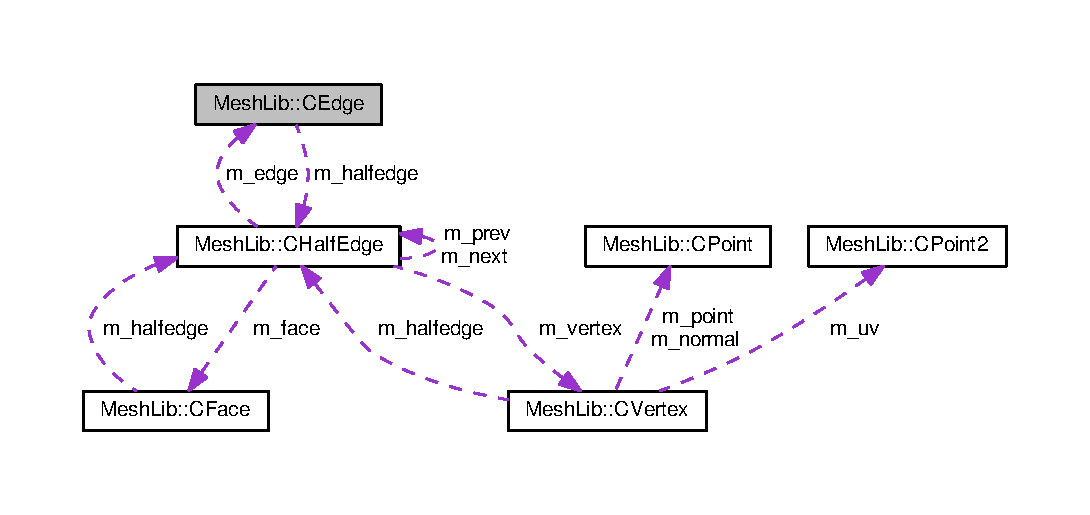
\includegraphics[width=350pt]{class_mesh_lib_1_1_c_edge__coll__graph}
\end{center}
\end{figure}
\subsection*{Public Member Functions}
\begin{DoxyCompactItemize}
\item 
\hyperlink{class_mesh_lib_1_1_c_edge_a513a0dc0e44f2592d516926c90763b67}{C\+Edge} ()
\item 
\hyperlink{class_mesh_lib_1_1_c_edge_a06f2cccf7d71658e397d83205f4a2c29}{$\sim$\+C\+Edge} ()
\item 
\hyperlink{class_mesh_lib_1_1_c_half_edge}{C\+Half\+Edge} $\ast$\& \hyperlink{class_mesh_lib_1_1_c_edge_a779a45a145714d9b177afb097ddfd5e6}{halfedge} (int id)
\item 
bool \hyperlink{class_mesh_lib_1_1_c_edge_a5fb31e9605d9f59fd89f74039bf4f9d9}{boundary} ()
\item 
\hyperlink{class_mesh_lib_1_1_c_half_edge}{C\+Half\+Edge} $\ast$\& \hyperlink{class_mesh_lib_1_1_c_edge_a5090261064156147ada856dea6e364f0}{other} (\hyperlink{class_mesh_lib_1_1_c_half_edge}{C\+Half\+Edge} $\ast$he)
\item 
std\+::string \& \hyperlink{class_mesh_lib_1_1_c_edge_a295387b2b8521e365312dbc2be90ec9a}{string} ()
\item 
void \hyperlink{class_mesh_lib_1_1_c_edge_a18e3af9e9a7dc8e6f60a2483bb19ad24}{\+\_\+from\+\_\+string} ()
\item 
void \hyperlink{class_mesh_lib_1_1_c_edge_a420d6973d64a53c21ef4dc15c557b36f}{\+\_\+to\+\_\+string} ()
\end{DoxyCompactItemize}
\subsection*{Protected Attributes}
\begin{DoxyCompactItemize}
\item 
\hyperlink{class_mesh_lib_1_1_c_half_edge}{C\+Half\+Edge} $\ast$ \hyperlink{class_mesh_lib_1_1_c_edge_a1d597f8d90c6c322ffbc5a454e7efb94}{m\+\_\+halfedge} \mbox{[}2\mbox{]}
\item 
std\+::string \hyperlink{class_mesh_lib_1_1_c_edge_a810f0a280e3a97d449386cc5cb6cce3b}{m\+\_\+string}
\end{DoxyCompactItemize}


\subsection{Detailed Description}
\hyperlink{class_mesh_lib_1_1_c_edge}{C\+Edge} class, which is the base class of all kinds of edge classes. 

Definition at line 26 of file Edge.\+h.



\subsection{Constructor \& Destructor Documentation}
\index{Mesh\+Lib\+::\+C\+Edge@{Mesh\+Lib\+::\+C\+Edge}!C\+Edge@{C\+Edge}}
\index{C\+Edge@{C\+Edge}!Mesh\+Lib\+::\+C\+Edge@{Mesh\+Lib\+::\+C\+Edge}}
\subsubsection[{\texorpdfstring{C\+Edge()}{CEdge()}}]{\setlength{\rightskip}{0pt plus 5cm}Mesh\+Lib\+::\+C\+Edge\+::\+C\+Edge (
\begin{DoxyParamCaption}
{}
\end{DoxyParamCaption}
)\hspace{0.3cm}{\ttfamily [inline]}}\hypertarget{class_mesh_lib_1_1_c_edge_a513a0dc0e44f2592d516926c90763b67}{}\label{class_mesh_lib_1_1_c_edge_a513a0dc0e44f2592d516926c90763b67}
\hyperlink{class_mesh_lib_1_1_c_edge}{C\+Edge} constructor, set both halfedge pointers to be N\+U\+LL. 

Definition at line 32 of file Edge.\+h.

\index{Mesh\+Lib\+::\+C\+Edge@{Mesh\+Lib\+::\+C\+Edge}!````~C\+Edge@{$\sim$\+C\+Edge}}
\index{````~C\+Edge@{$\sim$\+C\+Edge}!Mesh\+Lib\+::\+C\+Edge@{Mesh\+Lib\+::\+C\+Edge}}
\subsubsection[{\texorpdfstring{$\sim$\+C\+Edge()}{~CEdge()}}]{\setlength{\rightskip}{0pt plus 5cm}Mesh\+Lib\+::\+C\+Edge\+::$\sim$\+C\+Edge (
\begin{DoxyParamCaption}
{}
\end{DoxyParamCaption}
)\hspace{0.3cm}{\ttfamily [inline]}}\hypertarget{class_mesh_lib_1_1_c_edge_a06f2cccf7d71658e397d83205f4a2c29}{}\label{class_mesh_lib_1_1_c_edge_a06f2cccf7d71658e397d83205f4a2c29}
\hyperlink{class_mesh_lib_1_1_c_edge}{C\+Edge} destructor. 

Definition at line 36 of file Edge.\+h.



\subsection{Member Function Documentation}
\index{Mesh\+Lib\+::\+C\+Edge@{Mesh\+Lib\+::\+C\+Edge}!\+\_\+from\+\_\+string@{\+\_\+from\+\_\+string}}
\index{\+\_\+from\+\_\+string@{\+\_\+from\+\_\+string}!Mesh\+Lib\+::\+C\+Edge@{Mesh\+Lib\+::\+C\+Edge}}
\subsubsection[{\texorpdfstring{\+\_\+from\+\_\+string()}{_from_string()}}]{\setlength{\rightskip}{0pt plus 5cm}void Mesh\+Lib\+::\+C\+Edge\+::\+\_\+from\+\_\+string (
\begin{DoxyParamCaption}
{}
\end{DoxyParamCaption}
)\hspace{0.3cm}{\ttfamily [inline]}}\hypertarget{class_mesh_lib_1_1_c_edge_a18e3af9e9a7dc8e6f60a2483bb19ad24}{}\label{class_mesh_lib_1_1_c_edge_a18e3af9e9a7dc8e6f60a2483bb19ad24}
Read the traits from the string. 

Definition at line 61 of file Edge.\+h.

\index{Mesh\+Lib\+::\+C\+Edge@{Mesh\+Lib\+::\+C\+Edge}!\+\_\+to\+\_\+string@{\+\_\+to\+\_\+string}}
\index{\+\_\+to\+\_\+string@{\+\_\+to\+\_\+string}!Mesh\+Lib\+::\+C\+Edge@{Mesh\+Lib\+::\+C\+Edge}}
\subsubsection[{\texorpdfstring{\+\_\+to\+\_\+string()}{_to_string()}}]{\setlength{\rightskip}{0pt plus 5cm}void Mesh\+Lib\+::\+C\+Edge\+::\+\_\+to\+\_\+string (
\begin{DoxyParamCaption}
{}
\end{DoxyParamCaption}
)\hspace{0.3cm}{\ttfamily [inline]}}\hypertarget{class_mesh_lib_1_1_c_edge_a420d6973d64a53c21ef4dc15c557b36f}{}\label{class_mesh_lib_1_1_c_edge_a420d6973d64a53c21ef4dc15c557b36f}
Save the traits to the string. 

Definition at line 65 of file Edge.\+h.

\index{Mesh\+Lib\+::\+C\+Edge@{Mesh\+Lib\+::\+C\+Edge}!boundary@{boundary}}
\index{boundary@{boundary}!Mesh\+Lib\+::\+C\+Edge@{Mesh\+Lib\+::\+C\+Edge}}
\subsubsection[{\texorpdfstring{boundary()}{boundary()}}]{\setlength{\rightskip}{0pt plus 5cm}bool Mesh\+Lib\+::\+C\+Edge\+::boundary (
\begin{DoxyParamCaption}
{}
\end{DoxyParamCaption}
)\hspace{0.3cm}{\ttfamily [inline]}}\hypertarget{class_mesh_lib_1_1_c_edge_a5fb31e9605d9f59fd89f74039bf4f9d9}{}\label{class_mesh_lib_1_1_c_edge_a5fb31e9605d9f59fd89f74039bf4f9d9}
whether the edge is on the boundary. 

Definition at line 47 of file Edge.\+h.

\index{Mesh\+Lib\+::\+C\+Edge@{Mesh\+Lib\+::\+C\+Edge}!halfedge@{halfedge}}
\index{halfedge@{halfedge}!Mesh\+Lib\+::\+C\+Edge@{Mesh\+Lib\+::\+C\+Edge}}
\subsubsection[{\texorpdfstring{halfedge(int id)}{halfedge(int id)}}]{\setlength{\rightskip}{0pt plus 5cm}{\bf C\+Half\+Edge}$\ast$ \& Mesh\+Lib\+::\+C\+Edge\+::halfedge (
\begin{DoxyParamCaption}
\item[{int}]{id}
\end{DoxyParamCaption}
)\hspace{0.3cm}{\ttfamily [inline]}}\hypertarget{class_mesh_lib_1_1_c_edge_a779a45a145714d9b177afb097ddfd5e6}{}\label{class_mesh_lib_1_1_c_edge_a779a45a145714d9b177afb097ddfd5e6}
The halfedge attached to the current edge 
\begin{DoxyParams}{Parameters}
{\em id} & either 0 or 1 \\
\hline
\end{DoxyParams}
\begin{DoxyReturn}{Returns}
the halfedge\mbox{[}id\mbox{]} 
\end{DoxyReturn}


Definition at line 43 of file Edge.\+h.

\index{Mesh\+Lib\+::\+C\+Edge@{Mesh\+Lib\+::\+C\+Edge}!other@{other}}
\index{other@{other}!Mesh\+Lib\+::\+C\+Edge@{Mesh\+Lib\+::\+C\+Edge}}
\subsubsection[{\texorpdfstring{other(\+C\+Half\+Edge $\ast$he)}{other(CHalfEdge *he)}}]{\setlength{\rightskip}{0pt plus 5cm}{\bf C\+Half\+Edge}$\ast$ \& Mesh\+Lib\+::\+C\+Edge\+::other (
\begin{DoxyParamCaption}
\item[{{\bf C\+Half\+Edge} $\ast$}]{he}
\end{DoxyParamCaption}
)\hspace{0.3cm}{\ttfamily [inline]}}\hypertarget{class_mesh_lib_1_1_c_edge_a5090261064156147ada856dea6e364f0}{}\label{class_mesh_lib_1_1_c_edge_a5090261064156147ada856dea6e364f0}
The dual halfedge to the input halfedge 
\begin{DoxyParams}{Parameters}
{\em he} & halfedge attached to the current edge \\
\hline
\end{DoxyParams}
\begin{DoxyReturn}{Returns}
the other halfedge attached to the current edge 
\end{DoxyReturn}


Definition at line 53 of file Edge.\+h.

\index{Mesh\+Lib\+::\+C\+Edge@{Mesh\+Lib\+::\+C\+Edge}!string@{string}}
\index{string@{string}!Mesh\+Lib\+::\+C\+Edge@{Mesh\+Lib\+::\+C\+Edge}}
\subsubsection[{\texorpdfstring{string()}{string()}}]{\setlength{\rightskip}{0pt plus 5cm}std\+::string\& Mesh\+Lib\+::\+C\+Edge\+::string (
\begin{DoxyParamCaption}
{}
\end{DoxyParamCaption}
)\hspace{0.3cm}{\ttfamily [inline]}}\hypertarget{class_mesh_lib_1_1_c_edge_a295387b2b8521e365312dbc2be90ec9a}{}\label{class_mesh_lib_1_1_c_edge_a295387b2b8521e365312dbc2be90ec9a}
The string of the current edge. 

Definition at line 57 of file Edge.\+h.



\subsection{Member Data Documentation}
\index{Mesh\+Lib\+::\+C\+Edge@{Mesh\+Lib\+::\+C\+Edge}!m\+\_\+halfedge@{m\+\_\+halfedge}}
\index{m\+\_\+halfedge@{m\+\_\+halfedge}!Mesh\+Lib\+::\+C\+Edge@{Mesh\+Lib\+::\+C\+Edge}}
\subsubsection[{\texorpdfstring{m\+\_\+halfedge}{m_halfedge}}]{\setlength{\rightskip}{0pt plus 5cm}{\bf C\+Half\+Edge}$\ast$ Mesh\+Lib\+::\+C\+Edge\+::m\+\_\+halfedge\mbox{[}2\mbox{]}\hspace{0.3cm}{\ttfamily [protected]}}\hypertarget{class_mesh_lib_1_1_c_edge_a1d597f8d90c6c322ffbc5a454e7efb94}{}\label{class_mesh_lib_1_1_c_edge_a1d597f8d90c6c322ffbc5a454e7efb94}
Pointers to the two halfedges attached to the current edge. 

Definition at line 65 of file Edge.\+h.

\index{Mesh\+Lib\+::\+C\+Edge@{Mesh\+Lib\+::\+C\+Edge}!m\+\_\+string@{m\+\_\+string}}
\index{m\+\_\+string@{m\+\_\+string}!Mesh\+Lib\+::\+C\+Edge@{Mesh\+Lib\+::\+C\+Edge}}
\subsubsection[{\texorpdfstring{m\+\_\+string}{m_string}}]{\setlength{\rightskip}{0pt plus 5cm}std\+::string Mesh\+Lib\+::\+C\+Edge\+::m\+\_\+string\hspace{0.3cm}{\ttfamily [protected]}}\hypertarget{class_mesh_lib_1_1_c_edge_a810f0a280e3a97d449386cc5cb6cce3b}{}\label{class_mesh_lib_1_1_c_edge_a810f0a280e3a97d449386cc5cb6cce3b}
The string associated to the current edge. 

Definition at line 74 of file Edge.\+h.



The documentation for this class was generated from the following file\+:\begin{DoxyCompactItemize}
\item 
Mesh\+Lib/core/\+Mesh/\hyperlink{_edge_8h}{Edge.\+h}\end{DoxyCompactItemize}

\hypertarget{class_mesh_lib_1_1_c_euclidean_embed}{}\section{Mesh\+Lib\+:\+:C\+Euclidean\+Embed$<$ C\+Vertex, C\+Edge, C\+Face, C\+Half\+Edge $>$ Class Template Reference}
\label{class_mesh_lib_1_1_c_euclidean_embed}\index{Mesh\+Lib\+::\+C\+Euclidean\+Embed$<$ C\+Vertex, C\+Edge, C\+Face, C\+Half\+Edge $>$@{Mesh\+Lib\+::\+C\+Euclidean\+Embed$<$ C\+Vertex, C\+Edge, C\+Face, C\+Half\+Edge $>$}}


C\+Embed class.  




{\ttfamily \#include $<$Euclidean\+Embed.\+h$>$}



Inheritance diagram for Mesh\+Lib\+:\+:C\+Euclidean\+Embed$<$ C\+Vertex, C\+Edge, C\+Face, C\+Half\+Edge $>$\+:
\nopagebreak
\begin{figure}[H]
\begin{center}
\leavevmode
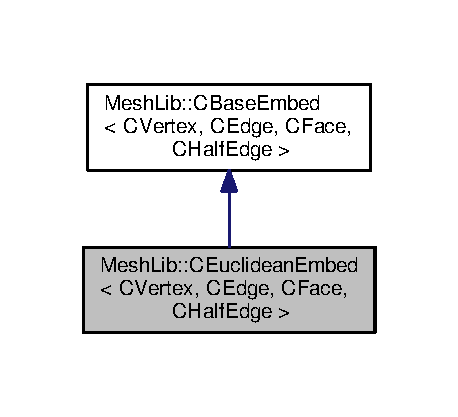
\includegraphics[width=220pt]{class_mesh_lib_1_1_c_euclidean_embed__inherit__graph}
\end{center}
\end{figure}


Collaboration diagram for Mesh\+Lib\+:\+:C\+Euclidean\+Embed$<$ C\+Vertex, C\+Edge, C\+Face, C\+Half\+Edge $>$\+:
\nopagebreak
\begin{figure}[H]
\begin{center}
\leavevmode
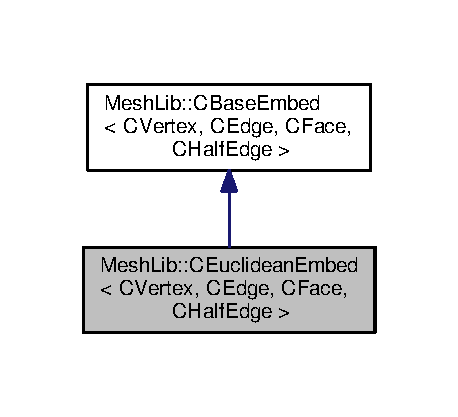
\includegraphics[width=220pt]{class_mesh_lib_1_1_c_euclidean_embed__coll__graph}
\end{center}
\end{figure}
\subsection*{Public Member Functions}
\begin{DoxyCompactItemize}
\item 
\hyperlink{class_mesh_lib_1_1_c_euclidean_embed_aaa1fcdae94b0186ceece3120d85e4520}{C\+Euclidean\+Embed} (C\+Ricci\+Flow\+Mesh$<$ \hyperlink{class_mesh_lib_1_1_c_vertex}{C\+Vertex}, \hyperlink{class_mesh_lib_1_1_c_edge}{C\+Edge}, \hyperlink{class_mesh_lib_1_1_c_face}{C\+Face}, \hyperlink{class_mesh_lib_1_1_c_half_edge}{C\+Half\+Edge} $>$ $\ast$p\+Mesh)
\begin{DoxyCompactList}\small\item\em \hyperlink{class_mesh_lib_1_1_c_euclidean_embed}{C\+Euclidean\+Embed} constructor. \end{DoxyCompactList}\item 
\hyperlink{class_mesh_lib_1_1_c_euclidean_embed_a6a4f24375f7c0cb1fce89dedef808605}{$\sim$\+C\+Euclidean\+Embed} ()
\begin{DoxyCompactList}\small\item\em \hyperlink{class_mesh_lib_1_1_c_euclidean_embed}{C\+Euclidean\+Embed} destructor. \end{DoxyCompactList}\end{DoxyCompactItemize}
\subsection*{Protected Member Functions}
\begin{DoxyCompactItemize}
\item 
void \hyperlink{class_mesh_lib_1_1_c_euclidean_embed_a6910ac47a9c2b101b8dca4049a533141}{\+\_\+embed\+\_\+first\+\_\+face} (\hyperlink{class_mesh_lib_1_1_c_face}{C\+Face} $\ast$head)
\item 
void \hyperlink{class_mesh_lib_1_1_c_euclidean_embed_aa77b6c218a33dbb01bc1eb5aad444c32}{\+\_\+embed\+\_\+face} (\hyperlink{class_mesh_lib_1_1_c_face}{C\+Face} $\ast$head)
\end{DoxyCompactItemize}
\subsection*{Additional Inherited Members}


\subsection{Detailed Description}
\subsubsection*{template$<$class C\+Vertex, class C\+Edge, class C\+Face, class C\+Half\+Edge$>$\\*
class Mesh\+Lib\+::\+C\+Euclidean\+Embed$<$ C\+Vertex, C\+Edge, C\+Face, C\+Half\+Edge $>$}

C\+Embed class. 

embed a mesh with flat metric onto the plane 

Definition at line 26 of file Euclidean\+Embed.\+h.



\subsection{Constructor \& Destructor Documentation}
\index{Mesh\+Lib\+::\+C\+Euclidean\+Embed@{Mesh\+Lib\+::\+C\+Euclidean\+Embed}!C\+Euclidean\+Embed@{C\+Euclidean\+Embed}}
\index{C\+Euclidean\+Embed@{C\+Euclidean\+Embed}!Mesh\+Lib\+::\+C\+Euclidean\+Embed@{Mesh\+Lib\+::\+C\+Euclidean\+Embed}}
\subsubsection[{\texorpdfstring{C\+Euclidean\+Embed(\+C\+Ricci\+Flow\+Mesh$<$ C\+Vertex, C\+Edge, C\+Face, C\+Half\+Edge $>$ $\ast$p\+Mesh)}{CEuclideanEmbed(CRicciFlowMesh< CVertex, CEdge, CFace, CHalfEdge > *pMesh)}}]{\setlength{\rightskip}{0pt plus 5cm}template$<$class C\+Vertex , class C\+Edge , class C\+Face , class C\+Half\+Edge $>$ {\bf Mesh\+Lib\+::\+C\+Euclidean\+Embed}$<$ {\bf C\+Vertex}, {\bf C\+Edge}, {\bf C\+Face}, {\bf C\+Half\+Edge} $>$\+::{\bf C\+Euclidean\+Embed} (
\begin{DoxyParamCaption}
\item[{C\+Ricci\+Flow\+Mesh$<$ {\bf C\+Vertex}, {\bf C\+Edge}, {\bf C\+Face}, {\bf C\+Half\+Edge} $>$ $\ast$}]{p\+Mesh}
\end{DoxyParamCaption}
)}\hypertarget{class_mesh_lib_1_1_c_euclidean_embed_aaa1fcdae94b0186ceece3120d85e4520}{}\label{class_mesh_lib_1_1_c_euclidean_embed_aaa1fcdae94b0186ceece3120d85e4520}


\hyperlink{class_mesh_lib_1_1_c_euclidean_embed}{C\+Euclidean\+Embed} constructor. 



Definition at line 50 of file Euclidean\+Embed.\+h.

\index{Mesh\+Lib\+::\+C\+Euclidean\+Embed@{Mesh\+Lib\+::\+C\+Euclidean\+Embed}!````~C\+Euclidean\+Embed@{$\sim$\+C\+Euclidean\+Embed}}
\index{````~C\+Euclidean\+Embed@{$\sim$\+C\+Euclidean\+Embed}!Mesh\+Lib\+::\+C\+Euclidean\+Embed@{Mesh\+Lib\+::\+C\+Euclidean\+Embed}}
\subsubsection[{\texorpdfstring{$\sim$\+C\+Euclidean\+Embed()}{~CEuclideanEmbed()}}]{\setlength{\rightskip}{0pt plus 5cm}template$<$class C\+Vertex , class C\+Edge , class C\+Face , class C\+Half\+Edge $>$ {\bf Mesh\+Lib\+::\+C\+Euclidean\+Embed}$<$ {\bf C\+Vertex}, {\bf C\+Edge}, {\bf C\+Face}, {\bf C\+Half\+Edge} $>$\+::$\sim${\bf C\+Euclidean\+Embed} (
\begin{DoxyParamCaption}
{}
\end{DoxyParamCaption}
)\hspace{0.3cm}{\ttfamily [inline]}}\hypertarget{class_mesh_lib_1_1_c_euclidean_embed_a6a4f24375f7c0cb1fce89dedef808605}{}\label{class_mesh_lib_1_1_c_euclidean_embed_a6a4f24375f7c0cb1fce89dedef808605}


\hyperlink{class_mesh_lib_1_1_c_euclidean_embed}{C\+Euclidean\+Embed} destructor. 



Definition at line 32 of file Euclidean\+Embed.\+h.



\subsection{Member Function Documentation}
\index{Mesh\+Lib\+::\+C\+Euclidean\+Embed@{Mesh\+Lib\+::\+C\+Euclidean\+Embed}!\+\_\+embed\+\_\+face@{\+\_\+embed\+\_\+face}}
\index{\+\_\+embed\+\_\+face@{\+\_\+embed\+\_\+face}!Mesh\+Lib\+::\+C\+Euclidean\+Embed@{Mesh\+Lib\+::\+C\+Euclidean\+Embed}}
\subsubsection[{\texorpdfstring{\+\_\+embed\+\_\+face(\+C\+Face $\ast$head)}{_embed_face(CFace *head)}}]{\setlength{\rightskip}{0pt plus 5cm}template$<$class C\+Vertex , class C\+Edge , class C\+Face , class C\+Half\+Edge $>$ void {\bf Mesh\+Lib\+::\+C\+Euclidean\+Embed}$<$ {\bf C\+Vertex}, {\bf C\+Edge}, {\bf C\+Face}, {\bf C\+Half\+Edge} $>$\+::\+\_\+embed\+\_\+face (
\begin{DoxyParamCaption}
\item[{{\bf C\+Face} $\ast$}]{head}
\end{DoxyParamCaption}
)\hspace{0.3cm}{\ttfamily [protected]}, {\ttfamily [virtual]}}\hypertarget{class_mesh_lib_1_1_c_euclidean_embed_aa77b6c218a33dbb01bc1eb5aad444c32}{}\label{class_mesh_lib_1_1_c_euclidean_embed_aa77b6c218a33dbb01bc1eb5aad444c32}
embed one face 

Implements \hyperlink{class_mesh_lib_1_1_c_base_embed_a41a602699326b590a718570141923258}{Mesh\+Lib\+::\+C\+Base\+Embed$<$ C\+Vertex, C\+Edge, C\+Face, C\+Half\+Edge $>$}.



Definition at line 104 of file Euclidean\+Embed.\+h.

\index{Mesh\+Lib\+::\+C\+Euclidean\+Embed@{Mesh\+Lib\+::\+C\+Euclidean\+Embed}!\+\_\+embed\+\_\+first\+\_\+face@{\+\_\+embed\+\_\+first\+\_\+face}}
\index{\+\_\+embed\+\_\+first\+\_\+face@{\+\_\+embed\+\_\+first\+\_\+face}!Mesh\+Lib\+::\+C\+Euclidean\+Embed@{Mesh\+Lib\+::\+C\+Euclidean\+Embed}}
\subsubsection[{\texorpdfstring{\+\_\+embed\+\_\+first\+\_\+face(\+C\+Face $\ast$head)}{_embed_first_face(CFace *head)}}]{\setlength{\rightskip}{0pt plus 5cm}template$<$class C\+Vertex , class C\+Edge , class C\+Face , class C\+Half\+Edge $>$ void {\bf Mesh\+Lib\+::\+C\+Euclidean\+Embed}$<$ {\bf C\+Vertex}, {\bf C\+Edge}, {\bf C\+Face}, {\bf C\+Half\+Edge} $>$\+::\+\_\+embed\+\_\+first\+\_\+face (
\begin{DoxyParamCaption}
\item[{{\bf C\+Face} $\ast$}]{head}
\end{DoxyParamCaption}
)\hspace{0.3cm}{\ttfamily [protected]}, {\ttfamily [virtual]}}\hypertarget{class_mesh_lib_1_1_c_euclidean_embed_a6910ac47a9c2b101b8dca4049a533141}{}\label{class_mesh_lib_1_1_c_euclidean_embed_a6910ac47a9c2b101b8dca4049a533141}
embed the first face 
\begin{DoxyParams}{Parameters}
{\em head} & the first face \\
\hline
\end{DoxyParams}


Implements \hyperlink{class_mesh_lib_1_1_c_base_embed_a1a05d4cad7181da5a1ccc66265609f89}{Mesh\+Lib\+::\+C\+Base\+Embed$<$ C\+Vertex, C\+Edge, C\+Face, C\+Half\+Edge $>$}.



Definition at line 57 of file Euclidean\+Embed.\+h.



The documentation for this class was generated from the following file\+:\begin{DoxyCompactItemize}
\item 
Mesh\+Lib/algorithm/\+Riemannian/\+Ricci\+Flow/\hyperlink{_euclidean_embed_8h}{Euclidean\+Embed.\+h}\end{DoxyCompactItemize}

\hypertarget{class_mesh_lib_1_1_c_face}{}\section{Mesh\+Lib\+:\+:C\+Face Class Reference}
\label{class_mesh_lib_1_1_c_face}\index{Mesh\+Lib\+::\+C\+Face@{Mesh\+Lib\+::\+C\+Face}}


\hyperlink{class_mesh_lib_1_1_c_face}{C\+Face} base class of all kinds of face classes.  




{\ttfamily \#include $<$Face.\+h$>$}



Collaboration diagram for Mesh\+Lib\+:\+:C\+Face\+:
\nopagebreak
\begin{figure}[H]
\begin{center}
\leavevmode
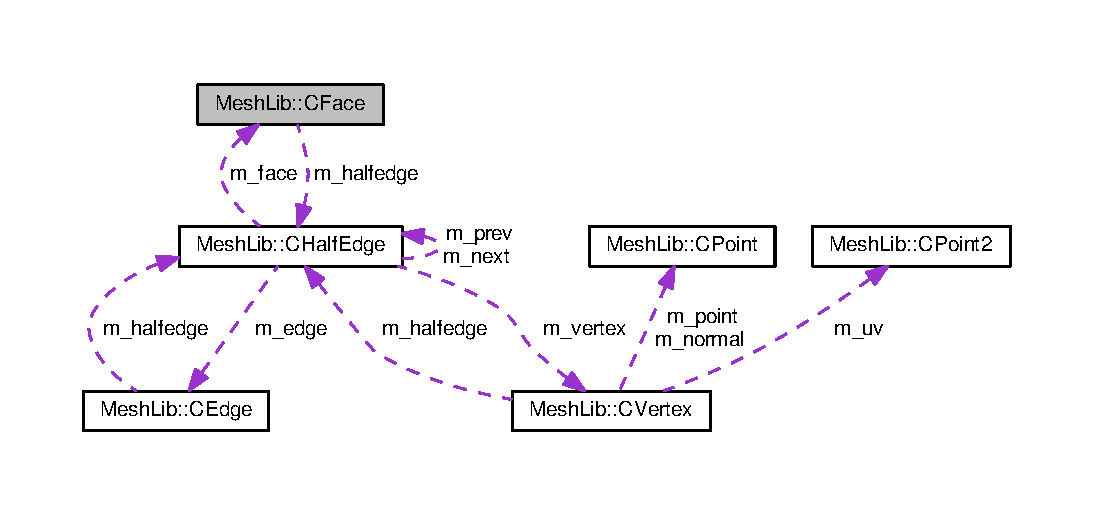
\includegraphics[width=350pt]{class_mesh_lib_1_1_c_face__coll__graph}
\end{center}
\end{figure}
\subsection*{Public Member Functions}
\begin{DoxyCompactItemize}
\item 
\hyperlink{class_mesh_lib_1_1_c_face_a3425979e07f04a516148a3e113ac7eab}{C\+Face} ()
\item 
\hyperlink{class_mesh_lib_1_1_c_face_a4146152b7902dad419181da0d23e74cb}{$\sim$\+C\+Face} ()
\item 
\hyperlink{class_mesh_lib_1_1_c_half_edge}{C\+Half\+Edge} $\ast$\& \hyperlink{class_mesh_lib_1_1_c_face_a6142ef04a531c8d364452db5ac3c7ba2}{halfedge} ()
\item 
int \& \hyperlink{class_mesh_lib_1_1_c_face_ae4eb0aaf069c3b17b324acfac47a66f0}{id} ()
\item 
const int \hyperlink{class_mesh_lib_1_1_c_face_a93c2cba1e9d3b986613b15e0e333909a}{id} () const 
\item 
std\+::string \& \hyperlink{class_mesh_lib_1_1_c_face_a2bedc65d146d2600d2c47d0aeb4233bb}{string} ()
\item 
void \hyperlink{class_mesh_lib_1_1_c_face_aa367b3ce68f1df45aa7dfdbd8e4ad1cb}{\+\_\+to\+\_\+string} ()
\item 
void \hyperlink{class_mesh_lib_1_1_c_face_a1470ee81803c0ca6a4cd29fcb4bc4925}{\+\_\+from\+\_\+string} ()
\end{DoxyCompactItemize}
\subsection*{Protected Attributes}
\begin{DoxyCompactItemize}
\item 
int \hyperlink{class_mesh_lib_1_1_c_face_ac8e8d0453e5e9882dc1ccbffea98734b}{m\+\_\+id}
\item 
\hyperlink{class_mesh_lib_1_1_c_half_edge}{C\+Half\+Edge} $\ast$ \hyperlink{class_mesh_lib_1_1_c_face_a583616821868cfcafc5cdfd1c5320f20}{m\+\_\+halfedge}
\item 
std\+::string \hyperlink{class_mesh_lib_1_1_c_face_afeb880ed9fa65f4e73f8f62c96ce347c}{m\+\_\+string}
\end{DoxyCompactItemize}


\subsection{Detailed Description}
\hyperlink{class_mesh_lib_1_1_c_face}{C\+Face} base class of all kinds of face classes. 

Definition at line 24 of file Face.\+h.



\subsection{Constructor \& Destructor Documentation}
\index{Mesh\+Lib\+::\+C\+Face@{Mesh\+Lib\+::\+C\+Face}!C\+Face@{C\+Face}}
\index{C\+Face@{C\+Face}!Mesh\+Lib\+::\+C\+Face@{Mesh\+Lib\+::\+C\+Face}}
\subsubsection[{\texorpdfstring{C\+Face()}{CFace()}}]{\setlength{\rightskip}{0pt plus 5cm}Mesh\+Lib\+::\+C\+Face\+::\+C\+Face (
\begin{DoxyParamCaption}
{}
\end{DoxyParamCaption}
)\hspace{0.3cm}{\ttfamily [inline]}}\hypertarget{class_mesh_lib_1_1_c_face_a3425979e07f04a516148a3e113ac7eab}{}\label{class_mesh_lib_1_1_c_face_a3425979e07f04a516148a3e113ac7eab}
\hyperlink{class_mesh_lib_1_1_c_face}{C\+Face} constructor 

Definition at line 30 of file Face.\+h.

\index{Mesh\+Lib\+::\+C\+Face@{Mesh\+Lib\+::\+C\+Face}!````~C\+Face@{$\sim$\+C\+Face}}
\index{````~C\+Face@{$\sim$\+C\+Face}!Mesh\+Lib\+::\+C\+Face@{Mesh\+Lib\+::\+C\+Face}}
\subsubsection[{\texorpdfstring{$\sim$\+C\+Face()}{~CFace()}}]{\setlength{\rightskip}{0pt plus 5cm}Mesh\+Lib\+::\+C\+Face\+::$\sim$\+C\+Face (
\begin{DoxyParamCaption}
{}
\end{DoxyParamCaption}
)\hspace{0.3cm}{\ttfamily [inline]}}\hypertarget{class_mesh_lib_1_1_c_face_a4146152b7902dad419181da0d23e74cb}{}\label{class_mesh_lib_1_1_c_face_a4146152b7902dad419181da0d23e74cb}
\hyperlink{class_mesh_lib_1_1_c_face}{C\+Face} destructor 

Definition at line 34 of file Face.\+h.



\subsection{Member Function Documentation}
\index{Mesh\+Lib\+::\+C\+Face@{Mesh\+Lib\+::\+C\+Face}!\+\_\+from\+\_\+string@{\+\_\+from\+\_\+string}}
\index{\+\_\+from\+\_\+string@{\+\_\+from\+\_\+string}!Mesh\+Lib\+::\+C\+Face@{Mesh\+Lib\+::\+C\+Face}}
\subsubsection[{\texorpdfstring{\+\_\+from\+\_\+string()}{_from_string()}}]{\setlength{\rightskip}{0pt plus 5cm}void Mesh\+Lib\+::\+C\+Face\+::\+\_\+from\+\_\+string (
\begin{DoxyParamCaption}
{}
\end{DoxyParamCaption}
)\hspace{0.3cm}{\ttfamily [inline]}}\hypertarget{class_mesh_lib_1_1_c_face_a1470ee81803c0ca6a4cd29fcb4bc4925}{}\label{class_mesh_lib_1_1_c_face_a1470ee81803c0ca6a4cd29fcb4bc4925}
read face traits from the string. 

Definition at line 58 of file Face.\+h.

\index{Mesh\+Lib\+::\+C\+Face@{Mesh\+Lib\+::\+C\+Face}!\+\_\+to\+\_\+string@{\+\_\+to\+\_\+string}}
\index{\+\_\+to\+\_\+string@{\+\_\+to\+\_\+string}!Mesh\+Lib\+::\+C\+Face@{Mesh\+Lib\+::\+C\+Face}}
\subsubsection[{\texorpdfstring{\+\_\+to\+\_\+string()}{_to_string()}}]{\setlength{\rightskip}{0pt plus 5cm}void Mesh\+Lib\+::\+C\+Face\+::\+\_\+to\+\_\+string (
\begin{DoxyParamCaption}
{}
\end{DoxyParamCaption}
)\hspace{0.3cm}{\ttfamily [inline]}}\hypertarget{class_mesh_lib_1_1_c_face_aa367b3ce68f1df45aa7dfdbd8e4ad1cb}{}\label{class_mesh_lib_1_1_c_face_aa367b3ce68f1df45aa7dfdbd8e4ad1cb}
Convert face traits to the string. 

Definition at line 54 of file Face.\+h.

\index{Mesh\+Lib\+::\+C\+Face@{Mesh\+Lib\+::\+C\+Face}!halfedge@{halfedge}}
\index{halfedge@{halfedge}!Mesh\+Lib\+::\+C\+Face@{Mesh\+Lib\+::\+C\+Face}}
\subsubsection[{\texorpdfstring{halfedge()}{halfedge()}}]{\setlength{\rightskip}{0pt plus 5cm}{\bf C\+Half\+Edge}$\ast$ \& Mesh\+Lib\+::\+C\+Face\+::halfedge (
\begin{DoxyParamCaption}
{}
\end{DoxyParamCaption}
)\hspace{0.3cm}{\ttfamily [inline]}}\hypertarget{class_mesh_lib_1_1_c_face_a6142ef04a531c8d364452db5ac3c7ba2}{}\label{class_mesh_lib_1_1_c_face_a6142ef04a531c8d364452db5ac3c7ba2}
One of the halfedges attaching to the current face. 

Definition at line 38 of file Face.\+h.

\index{Mesh\+Lib\+::\+C\+Face@{Mesh\+Lib\+::\+C\+Face}!id@{id}}
\index{id@{id}!Mesh\+Lib\+::\+C\+Face@{Mesh\+Lib\+::\+C\+Face}}
\subsubsection[{\texorpdfstring{id()}{id()}}]{\setlength{\rightskip}{0pt plus 5cm}int\& Mesh\+Lib\+::\+C\+Face\+::id (
\begin{DoxyParamCaption}
{}
\end{DoxyParamCaption}
)\hspace{0.3cm}{\ttfamily [inline]}}\hypertarget{class_mesh_lib_1_1_c_face_ae4eb0aaf069c3b17b324acfac47a66f0}{}\label{class_mesh_lib_1_1_c_face_ae4eb0aaf069c3b17b324acfac47a66f0}
The reference to the current face id 

Definition at line 42 of file Face.\+h.

\index{Mesh\+Lib\+::\+C\+Face@{Mesh\+Lib\+::\+C\+Face}!id@{id}}
\index{id@{id}!Mesh\+Lib\+::\+C\+Face@{Mesh\+Lib\+::\+C\+Face}}
\subsubsection[{\texorpdfstring{id() const }{id() const }}]{\setlength{\rightskip}{0pt plus 5cm}const int Mesh\+Lib\+::\+C\+Face\+::id (
\begin{DoxyParamCaption}
{}
\end{DoxyParamCaption}
) const\hspace{0.3cm}{\ttfamily [inline]}}\hypertarget{class_mesh_lib_1_1_c_face_a93c2cba1e9d3b986613b15e0e333909a}{}\label{class_mesh_lib_1_1_c_face_a93c2cba1e9d3b986613b15e0e333909a}
The value of the current face id. 

Definition at line 46 of file Face.\+h.

\index{Mesh\+Lib\+::\+C\+Face@{Mesh\+Lib\+::\+C\+Face}!string@{string}}
\index{string@{string}!Mesh\+Lib\+::\+C\+Face@{Mesh\+Lib\+::\+C\+Face}}
\subsubsection[{\texorpdfstring{string()}{string()}}]{\setlength{\rightskip}{0pt plus 5cm}std\+::string\& Mesh\+Lib\+::\+C\+Face\+::string (
\begin{DoxyParamCaption}
{}
\end{DoxyParamCaption}
)\hspace{0.3cm}{\ttfamily [inline]}}\hypertarget{class_mesh_lib_1_1_c_face_a2bedc65d146d2600d2c47d0aeb4233bb}{}\label{class_mesh_lib_1_1_c_face_a2bedc65d146d2600d2c47d0aeb4233bb}
The string of the current face. 

Definition at line 50 of file Face.\+h.



\subsection{Member Data Documentation}
\index{Mesh\+Lib\+::\+C\+Face@{Mesh\+Lib\+::\+C\+Face}!m\+\_\+halfedge@{m\+\_\+halfedge}}
\index{m\+\_\+halfedge@{m\+\_\+halfedge}!Mesh\+Lib\+::\+C\+Face@{Mesh\+Lib\+::\+C\+Face}}
\subsubsection[{\texorpdfstring{m\+\_\+halfedge}{m_halfedge}}]{\setlength{\rightskip}{0pt plus 5cm}{\bf C\+Half\+Edge}$\ast$ Mesh\+Lib\+::\+C\+Face\+::m\+\_\+halfedge\hspace{0.3cm}{\ttfamily [protected]}}\hypertarget{class_mesh_lib_1_1_c_face_a583616821868cfcafc5cdfd1c5320f20}{}\label{class_mesh_lib_1_1_c_face_a583616821868cfcafc5cdfd1c5320f20}
One halfedge attaching to the current face. 

Definition at line 67 of file Face.\+h.

\index{Mesh\+Lib\+::\+C\+Face@{Mesh\+Lib\+::\+C\+Face}!m\+\_\+id@{m\+\_\+id}}
\index{m\+\_\+id@{m\+\_\+id}!Mesh\+Lib\+::\+C\+Face@{Mesh\+Lib\+::\+C\+Face}}
\subsubsection[{\texorpdfstring{m\+\_\+id}{m_id}}]{\setlength{\rightskip}{0pt plus 5cm}int Mesh\+Lib\+::\+C\+Face\+::m\+\_\+id\hspace{0.3cm}{\ttfamily [protected]}}\hypertarget{class_mesh_lib_1_1_c_face_ac8e8d0453e5e9882dc1ccbffea98734b}{}\label{class_mesh_lib_1_1_c_face_ac8e8d0453e5e9882dc1ccbffea98734b}
id of the current face 

Definition at line 58 of file Face.\+h.

\index{Mesh\+Lib\+::\+C\+Face@{Mesh\+Lib\+::\+C\+Face}!m\+\_\+string@{m\+\_\+string}}
\index{m\+\_\+string@{m\+\_\+string}!Mesh\+Lib\+::\+C\+Face@{Mesh\+Lib\+::\+C\+Face}}
\subsubsection[{\texorpdfstring{m\+\_\+string}{m_string}}]{\setlength{\rightskip}{0pt plus 5cm}std\+::string Mesh\+Lib\+::\+C\+Face\+::m\+\_\+string\hspace{0.3cm}{\ttfamily [protected]}}\hypertarget{class_mesh_lib_1_1_c_face_afeb880ed9fa65f4e73f8f62c96ce347c}{}\label{class_mesh_lib_1_1_c_face_afeb880ed9fa65f4e73f8f62c96ce347c}
String of the current face. 

Definition at line 71 of file Face.\+h.



The documentation for this class was generated from the following file\+:\begin{DoxyCompactItemize}
\item 
Mesh\+Lib/core/\+Mesh/\hyperlink{_face_8h}{Face.\+h}\end{DoxyCompactItemize}

\hypertarget{class_mesh_lib_1_1_c_half_edge}{}\section{Mesh\+Lib\+:\+:C\+Half\+Edge Class Reference}
\label{class_mesh_lib_1_1_c_half_edge}\index{Mesh\+Lib\+::\+C\+Half\+Edge@{Mesh\+Lib\+::\+C\+Half\+Edge}}


\hyperlink{class_mesh_lib_1_1_c_half_edge}{C\+Half\+Edge} Base class of all kinds of halfedges.  




{\ttfamily \#include $<$Half\+Edge.\+h$>$}



Collaboration diagram for Mesh\+Lib\+:\+:C\+Half\+Edge\+:
\nopagebreak
\begin{figure}[H]
\begin{center}
\leavevmode
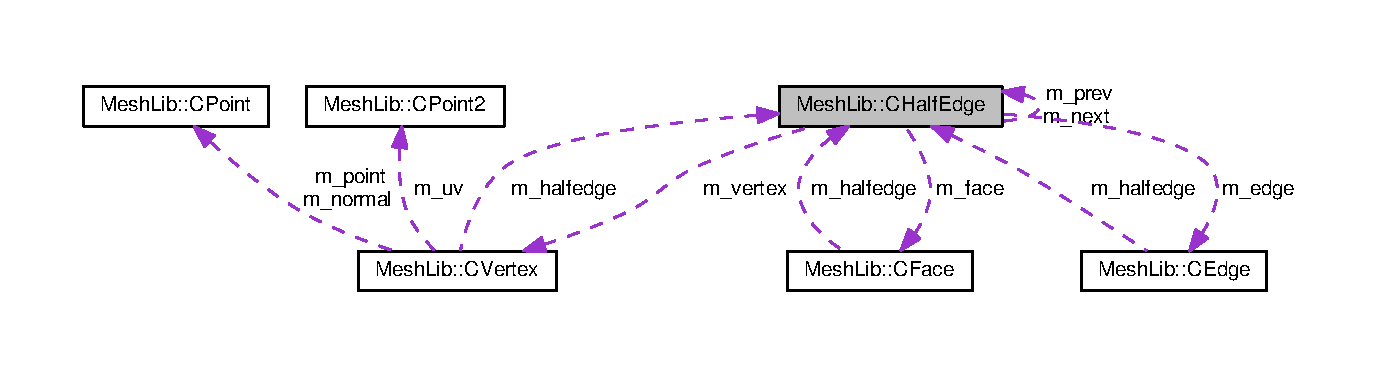
\includegraphics[width=350pt]{class_mesh_lib_1_1_c_half_edge__coll__graph}
\end{center}
\end{figure}
\subsection*{Public Member Functions}
\begin{DoxyCompactItemize}
\item 
\hyperlink{class_mesh_lib_1_1_c_half_edge_a9378ce34e4a19f08367911e64cd51e2d}{C\+Half\+Edge} ()
\item 
\hyperlink{class_mesh_lib_1_1_c_half_edge_a0e01e2c85afed1b7f58ecc45ee33e64f}{$\sim$\+C\+Half\+Edge} ()
\item 
\hyperlink{class_mesh_lib_1_1_c_edge}{C\+Edge} $\ast$\& \hyperlink{class_mesh_lib_1_1_c_half_edge_aa1724d1db29cd8757d5dee1d8153d684}{edge} ()
\item 
\hyperlink{class_mesh_lib_1_1_c_vertex}{C\+Vertex} $\ast$\& \hyperlink{class_mesh_lib_1_1_c_half_edge_a2063aaf2df1381ad2039fc439b6678a1}{vertex} ()
\item 
\hyperlink{class_mesh_lib_1_1_c_vertex}{C\+Vertex} $\ast$\& \hyperlink{class_mesh_lib_1_1_c_half_edge_a9485327b098c302b75b3174e7b089801}{target} ()
\item 
\hyperlink{class_mesh_lib_1_1_c_vertex}{C\+Vertex} $\ast$\& \hyperlink{class_mesh_lib_1_1_c_half_edge_a2948966fdbf42dd49dcb60db403d1d03}{source} ()
\item 
\hyperlink{class_mesh_lib_1_1_c_half_edge}{C\+Half\+Edge} $\ast$\& \hyperlink{class_mesh_lib_1_1_c_half_edge_a5b7e36ee2a8cf9429db2f245e1d37237}{he\+\_\+prev} ()
\item 
\hyperlink{class_mesh_lib_1_1_c_half_edge}{C\+Half\+Edge} $\ast$\& \hyperlink{class_mesh_lib_1_1_c_half_edge_afc73f6f23ef785403da61e77cf2d5ec7}{he\+\_\+next} ()
\item 
\hyperlink{class_mesh_lib_1_1_c_half_edge}{C\+Half\+Edge} $\ast$\& \hyperlink{class_mesh_lib_1_1_c_half_edge_a8498e670fe320824da2bd396c0467daa}{he\+\_\+sym} ()
\item 
\hyperlink{class_mesh_lib_1_1_c_face}{C\+Face} $\ast$\& \hyperlink{class_mesh_lib_1_1_c_half_edge_a3e959e63211e72cf1b78d58f644ef723}{face} ()
\item 
\hyperlink{class_mesh_lib_1_1_c_half_edge}{C\+Half\+Edge} $\ast$ \hyperlink{class_mesh_lib_1_1_c_half_edge_ab8c6cc91d89cd5f52ab9ef8202af1e90}{ccw\+\_\+rotate\+\_\+about\+\_\+target} ()
\item 
\hyperlink{class_mesh_lib_1_1_c_half_edge}{C\+Half\+Edge} $\ast$ \hyperlink{class_mesh_lib_1_1_c_half_edge_a82da051b8bdb4ebfd891ddf16e48049c}{clw\+\_\+rotate\+\_\+about\+\_\+target} ()
\item 
\hyperlink{class_mesh_lib_1_1_c_half_edge}{C\+Half\+Edge} $\ast$ \hyperlink{class_mesh_lib_1_1_c_half_edge_a3ccd9bdf3da946ead46ec5d9c25c6057}{ccw\+\_\+rotate\+\_\+about\+\_\+source} ()
\item 
\hyperlink{class_mesh_lib_1_1_c_half_edge}{C\+Half\+Edge} $\ast$ \hyperlink{class_mesh_lib_1_1_c_half_edge_ae286b5933152133439005627e6d793a9}{clw\+\_\+rotate\+\_\+about\+\_\+source} ()
\item 
std\+::string \& \hyperlink{class_mesh_lib_1_1_c_half_edge_a05f7de73fa51af4028748232854c97c5}{string} ()
\item 
void \hyperlink{class_mesh_lib_1_1_c_half_edge_a9122b66b6a23933f223bc6571141e745}{\+\_\+to\+\_\+string} ()
\item 
void \hyperlink{class_mesh_lib_1_1_c_half_edge_a95bb31440e3af2adb42f611c0c357882}{\+\_\+from\+\_\+string} ()
\end{DoxyCompactItemize}
\subsection*{Protected Attributes}
\begin{DoxyCompactItemize}
\item 
\hyperlink{class_mesh_lib_1_1_c_edge}{C\+Edge} $\ast$ \hyperlink{class_mesh_lib_1_1_c_half_edge_a881733f71ac3dd45d2ed7b587d70ee90}{m\+\_\+edge}
\item 
\hyperlink{class_mesh_lib_1_1_c_face}{C\+Face} $\ast$ \hyperlink{class_mesh_lib_1_1_c_half_edge_a46309154e53acc173e688a8fe1299ef9}{m\+\_\+face}
\item 
\hyperlink{class_mesh_lib_1_1_c_vertex}{C\+Vertex} $\ast$ \hyperlink{class_mesh_lib_1_1_c_half_edge_acaa06714b73d14153124be09a64236c0}{m\+\_\+vertex}
\item 
\hyperlink{class_mesh_lib_1_1_c_half_edge}{C\+Half\+Edge} $\ast$ \hyperlink{class_mesh_lib_1_1_c_half_edge_a7aaae52cda7d9cf2a18c42351c27b71e}{m\+\_\+prev}
\item 
\hyperlink{class_mesh_lib_1_1_c_half_edge}{C\+Half\+Edge} $\ast$ \hyperlink{class_mesh_lib_1_1_c_half_edge_ac9688abf74f8ab58b051fd2eb3895704}{m\+\_\+next}
\item 
std\+::string \hyperlink{class_mesh_lib_1_1_c_half_edge_a1b8813067a597ad547dc8e2a9405f653}{m\+\_\+string}
\end{DoxyCompactItemize}


\subsection{Detailed Description}
\hyperlink{class_mesh_lib_1_1_c_half_edge}{C\+Half\+Edge} Base class of all kinds of halfedges. 

Definition at line 26 of file Half\+Edge.\+h.



\subsection{Constructor \& Destructor Documentation}
\index{Mesh\+Lib\+::\+C\+Half\+Edge@{Mesh\+Lib\+::\+C\+Half\+Edge}!C\+Half\+Edge@{C\+Half\+Edge}}
\index{C\+Half\+Edge@{C\+Half\+Edge}!Mesh\+Lib\+::\+C\+Half\+Edge@{Mesh\+Lib\+::\+C\+Half\+Edge}}
\subsubsection[{\texorpdfstring{C\+Half\+Edge()}{CHalfEdge()}}]{\setlength{\rightskip}{0pt plus 5cm}Mesh\+Lib\+::\+C\+Half\+Edge\+::\+C\+Half\+Edge (
\begin{DoxyParamCaption}
{}
\end{DoxyParamCaption}
)\hspace{0.3cm}{\ttfamily [inline]}}\hypertarget{class_mesh_lib_1_1_c_half_edge_a9378ce34e4a19f08367911e64cd51e2d}{}\label{class_mesh_lib_1_1_c_half_edge_a9378ce34e4a19f08367911e64cd51e2d}
Constructor, initialize all pointers to be N\+U\+LL. 

Definition at line 32 of file Half\+Edge.\+h.

\index{Mesh\+Lib\+::\+C\+Half\+Edge@{Mesh\+Lib\+::\+C\+Half\+Edge}!````~C\+Half\+Edge@{$\sim$\+C\+Half\+Edge}}
\index{````~C\+Half\+Edge@{$\sim$\+C\+Half\+Edge}!Mesh\+Lib\+::\+C\+Half\+Edge@{Mesh\+Lib\+::\+C\+Half\+Edge}}
\subsubsection[{\texorpdfstring{$\sim$\+C\+Half\+Edge()}{~CHalfEdge()}}]{\setlength{\rightskip}{0pt plus 5cm}Mesh\+Lib\+::\+C\+Half\+Edge\+::$\sim$\+C\+Half\+Edge (
\begin{DoxyParamCaption}
{}
\end{DoxyParamCaption}
)\hspace{0.3cm}{\ttfamily [inline]}}\hypertarget{class_mesh_lib_1_1_c_half_edge_a0e01e2c85afed1b7f58ecc45ee33e64f}{}\label{class_mesh_lib_1_1_c_half_edge_a0e01e2c85afed1b7f58ecc45ee33e64f}
Destructure. 

Definition at line 35 of file Half\+Edge.\+h.



\subsection{Member Function Documentation}
\index{Mesh\+Lib\+::\+C\+Half\+Edge@{Mesh\+Lib\+::\+C\+Half\+Edge}!\+\_\+from\+\_\+string@{\+\_\+from\+\_\+string}}
\index{\+\_\+from\+\_\+string@{\+\_\+from\+\_\+string}!Mesh\+Lib\+::\+C\+Half\+Edge@{Mesh\+Lib\+::\+C\+Half\+Edge}}
\subsubsection[{\texorpdfstring{\+\_\+from\+\_\+string()}{_from_string()}}]{\setlength{\rightskip}{0pt plus 5cm}void Mesh\+Lib\+::\+C\+Half\+Edge\+::\+\_\+from\+\_\+string (
\begin{DoxyParamCaption}
{}
\end{DoxyParamCaption}
)\hspace{0.3cm}{\ttfamily [inline]}}\hypertarget{class_mesh_lib_1_1_c_half_edge_a95bb31440e3af2adb42f611c0c357882}{}\label{class_mesh_lib_1_1_c_half_edge_a95bb31440e3af2adb42f611c0c357882}
Read traits from string. 

Definition at line 74 of file Half\+Edge.\+h.

\index{Mesh\+Lib\+::\+C\+Half\+Edge@{Mesh\+Lib\+::\+C\+Half\+Edge}!\+\_\+to\+\_\+string@{\+\_\+to\+\_\+string}}
\index{\+\_\+to\+\_\+string@{\+\_\+to\+\_\+string}!Mesh\+Lib\+::\+C\+Half\+Edge@{Mesh\+Lib\+::\+C\+Half\+Edge}}
\subsubsection[{\texorpdfstring{\+\_\+to\+\_\+string()}{_to_string()}}]{\setlength{\rightskip}{0pt plus 5cm}void Mesh\+Lib\+::\+C\+Half\+Edge\+::\+\_\+to\+\_\+string (
\begin{DoxyParamCaption}
{}
\end{DoxyParamCaption}
)\hspace{0.3cm}{\ttfamily [inline]}}\hypertarget{class_mesh_lib_1_1_c_half_edge_a9122b66b6a23933f223bc6571141e745}{}\label{class_mesh_lib_1_1_c_half_edge_a9122b66b6a23933f223bc6571141e745}
Convert the traits to string. 

Definition at line 72 of file Half\+Edge.\+h.

\index{Mesh\+Lib\+::\+C\+Half\+Edge@{Mesh\+Lib\+::\+C\+Half\+Edge}!ccw\+\_\+rotate\+\_\+about\+\_\+source@{ccw\+\_\+rotate\+\_\+about\+\_\+source}}
\index{ccw\+\_\+rotate\+\_\+about\+\_\+source@{ccw\+\_\+rotate\+\_\+about\+\_\+source}!Mesh\+Lib\+::\+C\+Half\+Edge@{Mesh\+Lib\+::\+C\+Half\+Edge}}
\subsubsection[{\texorpdfstring{ccw\+\_\+rotate\+\_\+about\+\_\+source()}{ccw_rotate_about_source()}}]{\setlength{\rightskip}{0pt plus 5cm}{\bf C\+Half\+Edge} $\ast$ Mesh\+Lib\+::\+C\+Half\+Edge\+::ccw\+\_\+rotate\+\_\+about\+\_\+source (
\begin{DoxyParamCaption}
{}
\end{DoxyParamCaption}
)\hspace{0.3cm}{\ttfamily [inline]}}\hypertarget{class_mesh_lib_1_1_c_half_edge_a3ccd9bdf3da946ead46ec5d9c25c6057}{}\label{class_mesh_lib_1_1_c_half_edge_a3ccd9bdf3da946ead46ec5d9c25c6057}
Rotate the halfedge about the source vertex ccwly. \begin{DoxyReturn}{Returns}
if the current halfedge is the most ccw out halfedge of its source vertex, which is on boundary, return N\+U\+LL. 
\end{DoxyReturn}


Definition at line 112 of file Half\+Edge.\+h.

\index{Mesh\+Lib\+::\+C\+Half\+Edge@{Mesh\+Lib\+::\+C\+Half\+Edge}!ccw\+\_\+rotate\+\_\+about\+\_\+target@{ccw\+\_\+rotate\+\_\+about\+\_\+target}}
\index{ccw\+\_\+rotate\+\_\+about\+\_\+target@{ccw\+\_\+rotate\+\_\+about\+\_\+target}!Mesh\+Lib\+::\+C\+Half\+Edge@{Mesh\+Lib\+::\+C\+Half\+Edge}}
\subsubsection[{\texorpdfstring{ccw\+\_\+rotate\+\_\+about\+\_\+target()}{ccw_rotate_about_target()}}]{\setlength{\rightskip}{0pt plus 5cm}{\bf C\+Half\+Edge} $\ast$ Mesh\+Lib\+::\+C\+Half\+Edge\+::ccw\+\_\+rotate\+\_\+about\+\_\+target (
\begin{DoxyParamCaption}
{}
\end{DoxyParamCaption}
)\hspace{0.3cm}{\ttfamily [inline]}}\hypertarget{class_mesh_lib_1_1_c_half_edge_ab8c6cc91d89cd5f52ab9ef8202af1e90}{}\label{class_mesh_lib_1_1_c_half_edge_ab8c6cc91d89cd5f52ab9ef8202af1e90}
Rotate the halfedge about the target vertex ccwly. \begin{DoxyReturn}{Returns}
if the current halfedge is the most ccw in halfedge of its target vertex, which is on boundary, return N\+U\+LL. 
\end{DoxyReturn}


Definition at line 93 of file Half\+Edge.\+h.

\index{Mesh\+Lib\+::\+C\+Half\+Edge@{Mesh\+Lib\+::\+C\+Half\+Edge}!clw\+\_\+rotate\+\_\+about\+\_\+source@{clw\+\_\+rotate\+\_\+about\+\_\+source}}
\index{clw\+\_\+rotate\+\_\+about\+\_\+source@{clw\+\_\+rotate\+\_\+about\+\_\+source}!Mesh\+Lib\+::\+C\+Half\+Edge@{Mesh\+Lib\+::\+C\+Half\+Edge}}
\subsubsection[{\texorpdfstring{clw\+\_\+rotate\+\_\+about\+\_\+source()}{clw_rotate_about_source()}}]{\setlength{\rightskip}{0pt plus 5cm}{\bf C\+Half\+Edge} $\ast$ Mesh\+Lib\+::\+C\+Half\+Edge\+::clw\+\_\+rotate\+\_\+about\+\_\+source (
\begin{DoxyParamCaption}
{}
\end{DoxyParamCaption}
)\hspace{0.3cm}{\ttfamily [inline]}}\hypertarget{class_mesh_lib_1_1_c_half_edge_ae286b5933152133439005627e6d793a9}{}\label{class_mesh_lib_1_1_c_half_edge_ae286b5933152133439005627e6d793a9}
Rotate the halfedge about the source vertex ccwly. \begin{DoxyReturn}{Returns}
if the current halfedge is the most clw out halfedge of its source vertex, which is on boundary, return N\+U\+LL. 
\end{DoxyReturn}


Definition at line 121 of file Half\+Edge.\+h.

\index{Mesh\+Lib\+::\+C\+Half\+Edge@{Mesh\+Lib\+::\+C\+Half\+Edge}!clw\+\_\+rotate\+\_\+about\+\_\+target@{clw\+\_\+rotate\+\_\+about\+\_\+target}}
\index{clw\+\_\+rotate\+\_\+about\+\_\+target@{clw\+\_\+rotate\+\_\+about\+\_\+target}!Mesh\+Lib\+::\+C\+Half\+Edge@{Mesh\+Lib\+::\+C\+Half\+Edge}}
\subsubsection[{\texorpdfstring{clw\+\_\+rotate\+\_\+about\+\_\+target()}{clw_rotate_about_target()}}]{\setlength{\rightskip}{0pt plus 5cm}{\bf C\+Half\+Edge} $\ast$ Mesh\+Lib\+::\+C\+Half\+Edge\+::clw\+\_\+rotate\+\_\+about\+\_\+target (
\begin{DoxyParamCaption}
{}
\end{DoxyParamCaption}
)\hspace{0.3cm}{\ttfamily [inline]}}\hypertarget{class_mesh_lib_1_1_c_half_edge_a82da051b8bdb4ebfd891ddf16e48049c}{}\label{class_mesh_lib_1_1_c_half_edge_a82da051b8bdb4ebfd891ddf16e48049c}
Rotate the halfedge about the target vertex clwly. \begin{DoxyReturn}{Returns}
if the current halfedge is the most clw in halfedge of its target vertex, which is on boundary, return N\+U\+LL. 
\end{DoxyReturn}


Definition at line 103 of file Half\+Edge.\+h.

\index{Mesh\+Lib\+::\+C\+Half\+Edge@{Mesh\+Lib\+::\+C\+Half\+Edge}!edge@{edge}}
\index{edge@{edge}!Mesh\+Lib\+::\+C\+Half\+Edge@{Mesh\+Lib\+::\+C\+Half\+Edge}}
\subsubsection[{\texorpdfstring{edge()}{edge()}}]{\setlength{\rightskip}{0pt plus 5cm}{\bf C\+Edge}$\ast$ \& Mesh\+Lib\+::\+C\+Half\+Edge\+::edge (
\begin{DoxyParamCaption}
{}
\end{DoxyParamCaption}
)\hspace{0.3cm}{\ttfamily [inline]}}\hypertarget{class_mesh_lib_1_1_c_half_edge_aa1724d1db29cd8757d5dee1d8153d684}{}\label{class_mesh_lib_1_1_c_half_edge_aa1724d1db29cd8757d5dee1d8153d684}
Pointer to the edge attaching to the current halfedge. 

Definition at line 38 of file Half\+Edge.\+h.

\index{Mesh\+Lib\+::\+C\+Half\+Edge@{Mesh\+Lib\+::\+C\+Half\+Edge}!face@{face}}
\index{face@{face}!Mesh\+Lib\+::\+C\+Half\+Edge@{Mesh\+Lib\+::\+C\+Half\+Edge}}
\subsubsection[{\texorpdfstring{face()}{face()}}]{\setlength{\rightskip}{0pt plus 5cm}{\bf C\+Face}$\ast$ \& Mesh\+Lib\+::\+C\+Half\+Edge\+::face (
\begin{DoxyParamCaption}
{}
\end{DoxyParamCaption}
)\hspace{0.3cm}{\ttfamily [inline]}}\hypertarget{class_mesh_lib_1_1_c_half_edge_a3e959e63211e72cf1b78d58f644ef723}{}\label{class_mesh_lib_1_1_c_half_edge_a3e959e63211e72cf1b78d58f644ef723}
The face, to which the current halfedge attach. 

Definition at line 52 of file Half\+Edge.\+h.

\index{Mesh\+Lib\+::\+C\+Half\+Edge@{Mesh\+Lib\+::\+C\+Half\+Edge}!he\+\_\+next@{he\+\_\+next}}
\index{he\+\_\+next@{he\+\_\+next}!Mesh\+Lib\+::\+C\+Half\+Edge@{Mesh\+Lib\+::\+C\+Half\+Edge}}
\subsubsection[{\texorpdfstring{he\+\_\+next()}{he_next()}}]{\setlength{\rightskip}{0pt plus 5cm}{\bf C\+Half\+Edge}$\ast$ \& Mesh\+Lib\+::\+C\+Half\+Edge\+::he\+\_\+next (
\begin{DoxyParamCaption}
{}
\end{DoxyParamCaption}
)\hspace{0.3cm}{\ttfamily [inline]}}\hypertarget{class_mesh_lib_1_1_c_half_edge_afc73f6f23ef785403da61e77cf2d5ec7}{}\label{class_mesh_lib_1_1_c_half_edge_afc73f6f23ef785403da61e77cf2d5ec7}
Next halfedge of the current halfedge. 

Definition at line 48 of file Half\+Edge.\+h.

\index{Mesh\+Lib\+::\+C\+Half\+Edge@{Mesh\+Lib\+::\+C\+Half\+Edge}!he\+\_\+prev@{he\+\_\+prev}}
\index{he\+\_\+prev@{he\+\_\+prev}!Mesh\+Lib\+::\+C\+Half\+Edge@{Mesh\+Lib\+::\+C\+Half\+Edge}}
\subsubsection[{\texorpdfstring{he\+\_\+prev()}{he_prev()}}]{\setlength{\rightskip}{0pt plus 5cm}{\bf C\+Half\+Edge}$\ast$ \& Mesh\+Lib\+::\+C\+Half\+Edge\+::he\+\_\+prev (
\begin{DoxyParamCaption}
{}
\end{DoxyParamCaption}
)\hspace{0.3cm}{\ttfamily [inline]}}\hypertarget{class_mesh_lib_1_1_c_half_edge_a5b7e36ee2a8cf9429db2f245e1d37237}{}\label{class_mesh_lib_1_1_c_half_edge_a5b7e36ee2a8cf9429db2f245e1d37237}
Previous halfedge of the current halfedge. 

Definition at line 46 of file Half\+Edge.\+h.

\index{Mesh\+Lib\+::\+C\+Half\+Edge@{Mesh\+Lib\+::\+C\+Half\+Edge}!he\+\_\+sym@{he\+\_\+sym}}
\index{he\+\_\+sym@{he\+\_\+sym}!Mesh\+Lib\+::\+C\+Half\+Edge@{Mesh\+Lib\+::\+C\+Half\+Edge}}
\subsubsection[{\texorpdfstring{he\+\_\+sym()}{he_sym()}}]{\setlength{\rightskip}{0pt plus 5cm}{\bf C\+Half\+Edge}$\ast$ \& Mesh\+Lib\+::\+C\+Half\+Edge\+::he\+\_\+sym (
\begin{DoxyParamCaption}
{}
\end{DoxyParamCaption}
)\hspace{0.3cm}{\ttfamily [inline]}}\hypertarget{class_mesh_lib_1_1_c_half_edge_a8498e670fe320824da2bd396c0467daa}{}\label{class_mesh_lib_1_1_c_half_edge_a8498e670fe320824da2bd396c0467daa}
The dual halfedge of the current halfedge. 

Definition at line 50 of file Half\+Edge.\+h.

\index{Mesh\+Lib\+::\+C\+Half\+Edge@{Mesh\+Lib\+::\+C\+Half\+Edge}!source@{source}}
\index{source@{source}!Mesh\+Lib\+::\+C\+Half\+Edge@{Mesh\+Lib\+::\+C\+Half\+Edge}}
\subsubsection[{\texorpdfstring{source()}{source()}}]{\setlength{\rightskip}{0pt plus 5cm}{\bf C\+Vertex}$\ast$ \& Mesh\+Lib\+::\+C\+Half\+Edge\+::source (
\begin{DoxyParamCaption}
{}
\end{DoxyParamCaption}
)\hspace{0.3cm}{\ttfamily [inline]}}\hypertarget{class_mesh_lib_1_1_c_half_edge_a2948966fdbf42dd49dcb60db403d1d03}{}\label{class_mesh_lib_1_1_c_half_edge_a2948966fdbf42dd49dcb60db403d1d03}
Source vertex of the current halfedge. 

Definition at line 44 of file Half\+Edge.\+h.

\index{Mesh\+Lib\+::\+C\+Half\+Edge@{Mesh\+Lib\+::\+C\+Half\+Edge}!string@{string}}
\index{string@{string}!Mesh\+Lib\+::\+C\+Half\+Edge@{Mesh\+Lib\+::\+C\+Half\+Edge}}
\subsubsection[{\texorpdfstring{string()}{string()}}]{\setlength{\rightskip}{0pt plus 5cm}std\+::string\& Mesh\+Lib\+::\+C\+Half\+Edge\+::string (
\begin{DoxyParamCaption}
{}
\end{DoxyParamCaption}
)\hspace{0.3cm}{\ttfamily [inline]}}\hypertarget{class_mesh_lib_1_1_c_half_edge_a05f7de73fa51af4028748232854c97c5}{}\label{class_mesh_lib_1_1_c_half_edge_a05f7de73fa51af4028748232854c97c5}
String of the current halfedge. 

Definition at line 70 of file Half\+Edge.\+h.

\index{Mesh\+Lib\+::\+C\+Half\+Edge@{Mesh\+Lib\+::\+C\+Half\+Edge}!target@{target}}
\index{target@{target}!Mesh\+Lib\+::\+C\+Half\+Edge@{Mesh\+Lib\+::\+C\+Half\+Edge}}
\subsubsection[{\texorpdfstring{target()}{target()}}]{\setlength{\rightskip}{0pt plus 5cm}{\bf C\+Vertex}$\ast$ \& Mesh\+Lib\+::\+C\+Half\+Edge\+::target (
\begin{DoxyParamCaption}
{}
\end{DoxyParamCaption}
)\hspace{0.3cm}{\ttfamily [inline]}}\hypertarget{class_mesh_lib_1_1_c_half_edge_a9485327b098c302b75b3174e7b089801}{}\label{class_mesh_lib_1_1_c_half_edge_a9485327b098c302b75b3174e7b089801}
Target vertex of the current halfedge. 

Definition at line 42 of file Half\+Edge.\+h.

\index{Mesh\+Lib\+::\+C\+Half\+Edge@{Mesh\+Lib\+::\+C\+Half\+Edge}!vertex@{vertex}}
\index{vertex@{vertex}!Mesh\+Lib\+::\+C\+Half\+Edge@{Mesh\+Lib\+::\+C\+Half\+Edge}}
\subsubsection[{\texorpdfstring{vertex()}{vertex()}}]{\setlength{\rightskip}{0pt plus 5cm}{\bf C\+Vertex}$\ast$ \& Mesh\+Lib\+::\+C\+Half\+Edge\+::vertex (
\begin{DoxyParamCaption}
{}
\end{DoxyParamCaption}
)\hspace{0.3cm}{\ttfamily [inline]}}\hypertarget{class_mesh_lib_1_1_c_half_edge_a2063aaf2df1381ad2039fc439b6678a1}{}\label{class_mesh_lib_1_1_c_half_edge_a2063aaf2df1381ad2039fc439b6678a1}
Target vertex of the current halfedge. 

Definition at line 40 of file Half\+Edge.\+h.



\subsection{Member Data Documentation}
\index{Mesh\+Lib\+::\+C\+Half\+Edge@{Mesh\+Lib\+::\+C\+Half\+Edge}!m\+\_\+edge@{m\+\_\+edge}}
\index{m\+\_\+edge@{m\+\_\+edge}!Mesh\+Lib\+::\+C\+Half\+Edge@{Mesh\+Lib\+::\+C\+Half\+Edge}}
\subsubsection[{\texorpdfstring{m\+\_\+edge}{m_edge}}]{\setlength{\rightskip}{0pt plus 5cm}{\bf C\+Edge}$\ast$ Mesh\+Lib\+::\+C\+Half\+Edge\+::m\+\_\+edge\hspace{0.3cm}{\ttfamily [protected]}}\hypertarget{class_mesh_lib_1_1_c_half_edge_a881733f71ac3dd45d2ed7b587d70ee90}{}\label{class_mesh_lib_1_1_c_half_edge_a881733f71ac3dd45d2ed7b587d70ee90}
Edge, current halfedge attached to. 

Definition at line 74 of file Half\+Edge.\+h.

\index{Mesh\+Lib\+::\+C\+Half\+Edge@{Mesh\+Lib\+::\+C\+Half\+Edge}!m\+\_\+face@{m\+\_\+face}}
\index{m\+\_\+face@{m\+\_\+face}!Mesh\+Lib\+::\+C\+Half\+Edge@{Mesh\+Lib\+::\+C\+Half\+Edge}}
\subsubsection[{\texorpdfstring{m\+\_\+face}{m_face}}]{\setlength{\rightskip}{0pt plus 5cm}{\bf C\+Face}$\ast$ Mesh\+Lib\+::\+C\+Half\+Edge\+::m\+\_\+face\hspace{0.3cm}{\ttfamily [protected]}}\hypertarget{class_mesh_lib_1_1_c_half_edge_a46309154e53acc173e688a8fe1299ef9}{}\label{class_mesh_lib_1_1_c_half_edge_a46309154e53acc173e688a8fe1299ef9}
Face, current halfedge attached to. 

Definition at line 80 of file Half\+Edge.\+h.

\index{Mesh\+Lib\+::\+C\+Half\+Edge@{Mesh\+Lib\+::\+C\+Half\+Edge}!m\+\_\+next@{m\+\_\+next}}
\index{m\+\_\+next@{m\+\_\+next}!Mesh\+Lib\+::\+C\+Half\+Edge@{Mesh\+Lib\+::\+C\+Half\+Edge}}
\subsubsection[{\texorpdfstring{m\+\_\+next}{m_next}}]{\setlength{\rightskip}{0pt plus 5cm}{\bf C\+Half\+Edge}$\ast$ Mesh\+Lib\+::\+C\+Half\+Edge\+::m\+\_\+next\hspace{0.3cm}{\ttfamily [protected]}}\hypertarget{class_mesh_lib_1_1_c_half_edge_ac9688abf74f8ab58b051fd2eb3895704}{}\label{class_mesh_lib_1_1_c_half_edge_ac9688abf74f8ab58b051fd2eb3895704}
Next halfedge of the current halfedge, in the same face. 

Definition at line 86 of file Half\+Edge.\+h.

\index{Mesh\+Lib\+::\+C\+Half\+Edge@{Mesh\+Lib\+::\+C\+Half\+Edge}!m\+\_\+prev@{m\+\_\+prev}}
\index{m\+\_\+prev@{m\+\_\+prev}!Mesh\+Lib\+::\+C\+Half\+Edge@{Mesh\+Lib\+::\+C\+Half\+Edge}}
\subsubsection[{\texorpdfstring{m\+\_\+prev}{m_prev}}]{\setlength{\rightskip}{0pt plus 5cm}{\bf C\+Half\+Edge}$\ast$ Mesh\+Lib\+::\+C\+Half\+Edge\+::m\+\_\+prev\hspace{0.3cm}{\ttfamily [protected]}}\hypertarget{class_mesh_lib_1_1_c_half_edge_a7aaae52cda7d9cf2a18c42351c27b71e}{}\label{class_mesh_lib_1_1_c_half_edge_a7aaae52cda7d9cf2a18c42351c27b71e}
Previous halfedge of the current halfedge, in the same face. 

Definition at line 84 of file Half\+Edge.\+h.

\index{Mesh\+Lib\+::\+C\+Half\+Edge@{Mesh\+Lib\+::\+C\+Half\+Edge}!m\+\_\+string@{m\+\_\+string}}
\index{m\+\_\+string@{m\+\_\+string}!Mesh\+Lib\+::\+C\+Half\+Edge@{Mesh\+Lib\+::\+C\+Half\+Edge}}
\subsubsection[{\texorpdfstring{m\+\_\+string}{m_string}}]{\setlength{\rightskip}{0pt plus 5cm}std\+::string Mesh\+Lib\+::\+C\+Half\+Edge\+::m\+\_\+string\hspace{0.3cm}{\ttfamily [protected]}}\hypertarget{class_mesh_lib_1_1_c_half_edge_a1b8813067a597ad547dc8e2a9405f653}{}\label{class_mesh_lib_1_1_c_half_edge_a1b8813067a597ad547dc8e2a9405f653}
The string of the current halfedge. 

Definition at line 88 of file Half\+Edge.\+h.

\index{Mesh\+Lib\+::\+C\+Half\+Edge@{Mesh\+Lib\+::\+C\+Half\+Edge}!m\+\_\+vertex@{m\+\_\+vertex}}
\index{m\+\_\+vertex@{m\+\_\+vertex}!Mesh\+Lib\+::\+C\+Half\+Edge@{Mesh\+Lib\+::\+C\+Half\+Edge}}
\subsubsection[{\texorpdfstring{m\+\_\+vertex}{m_vertex}}]{\setlength{\rightskip}{0pt plus 5cm}{\bf C\+Vertex}$\ast$ Mesh\+Lib\+::\+C\+Half\+Edge\+::m\+\_\+vertex\hspace{0.3cm}{\ttfamily [protected]}}\hypertarget{class_mesh_lib_1_1_c_half_edge_acaa06714b73d14153124be09a64236c0}{}\label{class_mesh_lib_1_1_c_half_edge_acaa06714b73d14153124be09a64236c0}
Target vertex of the current halfedge. 

Definition at line 82 of file Half\+Edge.\+h.



The documentation for this class was generated from the following file\+:\begin{DoxyCompactItemize}
\item 
Mesh\+Lib/core/\+Mesh/\hyperlink{_half_edge_8h}{Half\+Edge.\+h}\end{DoxyCompactItemize}

\hypertarget{class_mesh_lib_1_1_c_loop}{}\section{Mesh\+Lib\+:\+:C\+Loop$<$ C\+Vertex, C\+Edge, C\+Face, C\+Half\+Edge $>$ Class Template Reference}
\label{class_mesh_lib_1_1_c_loop}\index{Mesh\+Lib\+::\+C\+Loop$<$ C\+Vertex, C\+Edge, C\+Face, C\+Half\+Edge $>$@{Mesh\+Lib\+::\+C\+Loop$<$ C\+Vertex, C\+Edge, C\+Face, C\+Half\+Edge $>$}}


\hyperlink{class_mesh_lib_1_1_c_loop}{C\+Loop} Boundary loop class.  




{\ttfamily \#include $<$boundary.\+h$>$}



Collaboration diagram for Mesh\+Lib\+:\+:C\+Loop$<$ C\+Vertex, C\+Edge, C\+Face, C\+Half\+Edge $>$\+:
\nopagebreak
\begin{figure}[H]
\begin{center}
\leavevmode
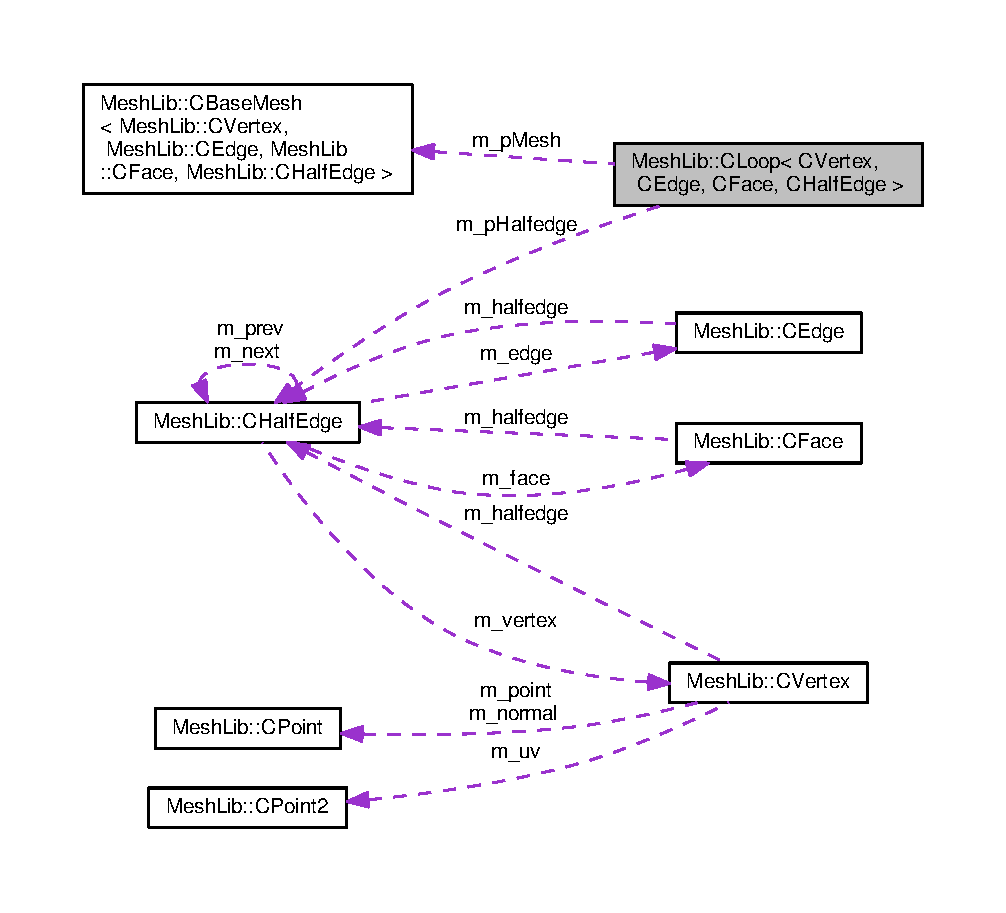
\includegraphics[width=350pt]{class_mesh_lib_1_1_c_loop__coll__graph}
\end{center}
\end{figure}
\subsection*{Public Member Functions}
\begin{DoxyCompactItemize}
\item 
\hyperlink{class_mesh_lib_1_1_c_loop_ab5608d60065d49d97e7ab5173b84c8b6}{C\+Loop} (\hyperlink{class_mesh_lib_1_1_c_base_mesh}{C\+Base\+Mesh}$<$ \hyperlink{class_mesh_lib_1_1_c_vertex}{C\+Vertex}, \hyperlink{class_mesh_lib_1_1_c_edge}{C\+Edge}, \hyperlink{class_mesh_lib_1_1_c_face}{C\+Face}, \hyperlink{class_mesh_lib_1_1_c_half_edge}{C\+Half\+Edge} $>$ $\ast$p\+Mesh, \hyperlink{class_mesh_lib_1_1_c_half_edge}{C\+Half\+Edge} $\ast$pH)
\item 
\hyperlink{class_mesh_lib_1_1_c_loop_ab3142314d0e6fefd57fd4a6339fd86cf}{C\+Loop} (\hyperlink{class_mesh_lib_1_1_c_base_mesh}{C\+Base\+Mesh}$<$ \hyperlink{class_mesh_lib_1_1_c_vertex}{C\+Vertex}, \hyperlink{class_mesh_lib_1_1_c_edge}{C\+Edge}, \hyperlink{class_mesh_lib_1_1_c_face}{C\+Face}, \hyperlink{class_mesh_lib_1_1_c_half_edge}{C\+Half\+Edge} $>$ $\ast$p\+Mesh)
\item 
\hyperlink{class_mesh_lib_1_1_c_loop_a167b5a15311a3c0bc8a676316894595d}{$\sim$\+C\+Loop} ()
\item 
std\+::list$<$ \hyperlink{class_mesh_lib_1_1_c_half_edge}{C\+Half\+Edge} $\ast$ $>$ \& \hyperlink{class_mesh_lib_1_1_c_loop_a77fea4b74d23423e5889f2046d997cbf}{halfedges} ()
\item 
double \hyperlink{class_mesh_lib_1_1_c_loop_af56b2cace83571be3b745528e8985131}{length} ()
\item 
void \hyperlink{class_mesh_lib_1_1_c_loop_a86a97b1d9b30030dd5b04544cb1052c4}{write} (const char $\ast$file)
\item 
void \hyperlink{class_mesh_lib_1_1_c_loop_a200d03806ae46c7afed2bca200298487}{read} (const char $\ast$file)
\end{DoxyCompactItemize}
\subsection*{Protected Attributes}
\begin{DoxyCompactItemize}
\item 
\hyperlink{class_mesh_lib_1_1_c_base_mesh}{C\+Base\+Mesh}$<$ \hyperlink{class_mesh_lib_1_1_c_vertex}{C\+Vertex}, \hyperlink{class_mesh_lib_1_1_c_edge}{C\+Edge}, \hyperlink{class_mesh_lib_1_1_c_face}{C\+Face}, \hyperlink{class_mesh_lib_1_1_c_half_edge}{C\+Half\+Edge} $>$ $\ast$ \hyperlink{class_mesh_lib_1_1_c_loop_a4656ced7a75ac9a63bc5925bb667ee55}{m\+\_\+p\+Mesh}
\item 
double \hyperlink{class_mesh_lib_1_1_c_loop_a3886caa41e199204666ca08dcf90f847}{m\+\_\+length}
\item 
\hyperlink{class_mesh_lib_1_1_c_half_edge}{C\+Half\+Edge} $\ast$ \hyperlink{class_mesh_lib_1_1_c_loop_ad8bcb68b8cafda18031803a855b1c47a}{m\+\_\+p\+Halfedge}
\item 
std\+::list$<$ \hyperlink{class_mesh_lib_1_1_c_half_edge}{C\+Half\+Edge} $\ast$ $>$ \hyperlink{class_mesh_lib_1_1_c_loop_a52708198f9b27b7aba3f3df30f46bb5e}{m\+\_\+halfedges}
\end{DoxyCompactItemize}


\subsection{Detailed Description}
\subsubsection*{template$<$class C\+Vertex, class C\+Edge, class C\+Face, class C\+Half\+Edge$>$\\*
class Mesh\+Lib\+::\+C\+Loop$<$ C\+Vertex, C\+Edge, C\+Face, C\+Half\+Edge $>$}

\hyperlink{class_mesh_lib_1_1_c_loop}{C\+Loop} Boundary loop class. 


\begin{DoxyTemplParams}{Template Parameters}
{\em \hyperlink{class_mesh_lib_1_1_c_vertex}{C\+Vertex}} & Vertex type \\
\hline
{\em \hyperlink{class_mesh_lib_1_1_c_edge}{C\+Edge}} & Edge type \\
\hline
{\em \hyperlink{class_mesh_lib_1_1_c_face}{C\+Face}} & Face type \\
\hline
{\em \hyperlink{class_mesh_lib_1_1_c_half_edge}{C\+Half\+Edge}} & Half\+Edge type \\
\hline
\end{DoxyTemplParams}


Definition at line 35 of file boundary.\+h.



\subsection{Constructor \& Destructor Documentation}
\index{Mesh\+Lib\+::\+C\+Loop@{Mesh\+Lib\+::\+C\+Loop}!C\+Loop@{C\+Loop}}
\index{C\+Loop@{C\+Loop}!Mesh\+Lib\+::\+C\+Loop@{Mesh\+Lib\+::\+C\+Loop}}
\subsubsection[{\texorpdfstring{C\+Loop(\+C\+Base\+Mesh$<$ C\+Vertex, C\+Edge, C\+Face, C\+Half\+Edge $>$ $\ast$p\+Mesh, C\+Half\+Edge $\ast$p\+H)}{CLoop(CBaseMesh< CVertex, CEdge, CFace, CHalfEdge > *pMesh, CHalfEdge *pH)}}]{\setlength{\rightskip}{0pt plus 5cm}template$<$class C\+Vertex , class C\+Edge , class C\+Face , class C\+Half\+Edge $>$ {\bf Mesh\+Lib\+::\+C\+Loop}$<$ {\bf C\+Vertex}, {\bf C\+Edge}, {\bf C\+Face}, {\bf C\+Half\+Edge} $>$\+::{\bf C\+Loop} (
\begin{DoxyParamCaption}
\item[{{\bf C\+Base\+Mesh}$<$ {\bf C\+Vertex}, {\bf C\+Edge}, {\bf C\+Face}, {\bf C\+Half\+Edge} $>$ $\ast$}]{p\+Mesh, }
\item[{{\bf C\+Half\+Edge} $\ast$}]{pH}
\end{DoxyParamCaption}
)}\hypertarget{class_mesh_lib_1_1_c_loop_ab5608d60065d49d97e7ab5173b84c8b6}{}\label{class_mesh_lib_1_1_c_loop_ab5608d60065d49d97e7ab5173b84c8b6}
Constructor of the \hyperlink{class_mesh_lib_1_1_c_loop}{C\+Loop} 
\begin{DoxyParams}{Parameters}
{\em p\+Mesh} & pointer to the current mesh \\
\hline
{\em pH} & halfedge on the boundary loop\\
\hline
\end{DoxyParams}
\hyperlink{class_mesh_lib_1_1_c_loop}{C\+Loop} constructure, trace the boundary loop, starting from the halfedge pH. 
\begin{DoxyParams}{Parameters}
{\em p\+Mesh} & pointer to the current mesh \\
\hline
{\em pH} & halfedge on the current boundary loop \\
\hline
\end{DoxyParams}


Definition at line 152 of file boundary.\+h.

\index{Mesh\+Lib\+::\+C\+Loop@{Mesh\+Lib\+::\+C\+Loop}!C\+Loop@{C\+Loop}}
\index{C\+Loop@{C\+Loop}!Mesh\+Lib\+::\+C\+Loop@{Mesh\+Lib\+::\+C\+Loop}}
\subsubsection[{\texorpdfstring{C\+Loop(\+C\+Base\+Mesh$<$ C\+Vertex, C\+Edge, C\+Face, C\+Half\+Edge $>$ $\ast$p\+Mesh)}{CLoop(CBaseMesh< CVertex, CEdge, CFace, CHalfEdge > *pMesh)}}]{\setlength{\rightskip}{0pt plus 5cm}template$<$class C\+Vertex, class C\+Edge, class C\+Face, class C\+Half\+Edge$>$ {\bf Mesh\+Lib\+::\+C\+Loop}$<$ {\bf C\+Vertex}, {\bf C\+Edge}, {\bf C\+Face}, {\bf C\+Half\+Edge} $>$\+::{\bf C\+Loop} (
\begin{DoxyParamCaption}
\item[{{\bf C\+Base\+Mesh}$<$ {\bf C\+Vertex}, {\bf C\+Edge}, {\bf C\+Face}, {\bf C\+Half\+Edge} $>$ $\ast$}]{p\+Mesh}
\end{DoxyParamCaption}
)\hspace{0.3cm}{\ttfamily [inline]}}\hypertarget{class_mesh_lib_1_1_c_loop_ab3142314d0e6fefd57fd4a6339fd86cf}{}\label{class_mesh_lib_1_1_c_loop_ab3142314d0e6fefd57fd4a6339fd86cf}
Constructor of the \hyperlink{class_mesh_lib_1_1_c_loop}{C\+Loop} 
\begin{DoxyParams}{Parameters}
{\em p\+Mesh} & pointer to the current mesh \\
\hline
\end{DoxyParams}


Definition at line 48 of file boundary.\+h.

\index{Mesh\+Lib\+::\+C\+Loop@{Mesh\+Lib\+::\+C\+Loop}!````~C\+Loop@{$\sim$\+C\+Loop}}
\index{````~C\+Loop@{$\sim$\+C\+Loop}!Mesh\+Lib\+::\+C\+Loop@{Mesh\+Lib\+::\+C\+Loop}}
\subsubsection[{\texorpdfstring{$\sim$\+C\+Loop()}{~CLoop()}}]{\setlength{\rightskip}{0pt plus 5cm}template$<$class C\+Vertex , class C\+Edge , class C\+Face , class C\+Half\+Edge $>$ {\bf Mesh\+Lib\+::\+C\+Loop}$<$ {\bf C\+Vertex}, {\bf C\+Edge}, {\bf C\+Face}, {\bf C\+Half\+Edge} $>$\+::$\sim${\bf C\+Loop} (
\begin{DoxyParamCaption}
{}
\end{DoxyParamCaption}
)}\hypertarget{class_mesh_lib_1_1_c_loop_a167b5a15311a3c0bc8a676316894595d}{}\label{class_mesh_lib_1_1_c_loop_a167b5a15311a3c0bc8a676316894595d}
Destructor of \hyperlink{class_mesh_lib_1_1_c_loop}{C\+Loop}.

\hyperlink{class_mesh_lib_1_1_c_loop}{C\+Loop} destructor, clean up the list of halfedges in the loop 

Definition at line 173 of file boundary.\+h.



\subsection{Member Function Documentation}
\index{Mesh\+Lib\+::\+C\+Loop@{Mesh\+Lib\+::\+C\+Loop}!halfedges@{halfedges}}
\index{halfedges@{halfedges}!Mesh\+Lib\+::\+C\+Loop@{Mesh\+Lib\+::\+C\+Loop}}
\subsubsection[{\texorpdfstring{halfedges()}{halfedges()}}]{\setlength{\rightskip}{0pt plus 5cm}template$<$class C\+Vertex, class C\+Edge, class C\+Face, class C\+Half\+Edge$>$ std\+::list$<${\bf C\+Half\+Edge}$\ast$$>$\& {\bf Mesh\+Lib\+::\+C\+Loop}$<$ {\bf C\+Vertex}, {\bf C\+Edge}, {\bf C\+Face}, {\bf C\+Half\+Edge} $>$\+::halfedges (
\begin{DoxyParamCaption}
{}
\end{DoxyParamCaption}
)\hspace{0.3cm}{\ttfamily [inline]}}\hypertarget{class_mesh_lib_1_1_c_loop_a77fea4b74d23423e5889f2046d997cbf}{}\label{class_mesh_lib_1_1_c_loop_a77fea4b74d23423e5889f2046d997cbf}
The list of haledges on the current boundary loop. 

Definition at line 57 of file boundary.\+h.

\index{Mesh\+Lib\+::\+C\+Loop@{Mesh\+Lib\+::\+C\+Loop}!length@{length}}
\index{length@{length}!Mesh\+Lib\+::\+C\+Loop@{Mesh\+Lib\+::\+C\+Loop}}
\subsubsection[{\texorpdfstring{length()}{length()}}]{\setlength{\rightskip}{0pt plus 5cm}template$<$class C\+Vertex, class C\+Edge, class C\+Face, class C\+Half\+Edge$>$ double {\bf Mesh\+Lib\+::\+C\+Loop}$<$ {\bf C\+Vertex}, {\bf C\+Edge}, {\bf C\+Face}, {\bf C\+Half\+Edge} $>$\+::length (
\begin{DoxyParamCaption}
{}
\end{DoxyParamCaption}
)\hspace{0.3cm}{\ttfamily [inline]}}\hypertarget{class_mesh_lib_1_1_c_loop_af56b2cace83571be3b745528e8985131}{}\label{class_mesh_lib_1_1_c_loop_af56b2cace83571be3b745528e8985131}
The length of the current boundary loop. 

Definition at line 65 of file boundary.\+h.

\index{Mesh\+Lib\+::\+C\+Loop@{Mesh\+Lib\+::\+C\+Loop}!read@{read}}
\index{read@{read}!Mesh\+Lib\+::\+C\+Loop@{Mesh\+Lib\+::\+C\+Loop}}
\subsubsection[{\texorpdfstring{read(const char $\ast$file)}{read(const char *file)}}]{\setlength{\rightskip}{0pt plus 5cm}template$<$class C\+Vertex , class C\+Edge , class C\+Face , class C\+Half\+Edge $>$ void {\bf Mesh\+Lib\+::\+C\+Loop}$<$ {\bf C\+Vertex}, {\bf C\+Edge}, {\bf C\+Face}, {\bf C\+Half\+Edge} $>$\+::read (
\begin{DoxyParamCaption}
\item[{const char $\ast$}]{file\+\_\+name}
\end{DoxyParamCaption}
)}\hypertarget{class_mesh_lib_1_1_c_loop_a200d03806ae46c7afed2bca200298487}{}\label{class_mesh_lib_1_1_c_loop_a200d03806ae46c7afed2bca200298487}
Input from a file

Output the loop to a file 
\begin{DoxyParams}{Parameters}
{\em file\+\_\+name} & the name of the file \\
\hline
\end{DoxyParams}


Definition at line 290 of file boundary.\+h.

\index{Mesh\+Lib\+::\+C\+Loop@{Mesh\+Lib\+::\+C\+Loop}!write@{write}}
\index{write@{write}!Mesh\+Lib\+::\+C\+Loop@{Mesh\+Lib\+::\+C\+Loop}}
\subsubsection[{\texorpdfstring{write(const char $\ast$file)}{write(const char *file)}}]{\setlength{\rightskip}{0pt plus 5cm}template$<$class C\+Vertex , class C\+Edge , class C\+Face , class C\+Half\+Edge $>$ void {\bf Mesh\+Lib\+::\+C\+Loop}$<$ {\bf C\+Vertex}, {\bf C\+Edge}, {\bf C\+Face}, {\bf C\+Half\+Edge} $>$\+::write (
\begin{DoxyParamCaption}
\item[{const char $\ast$}]{file\+\_\+name}
\end{DoxyParamCaption}
)}\hypertarget{class_mesh_lib_1_1_c_loop_a86a97b1d9b30030dd5b04544cb1052c4}{}\label{class_mesh_lib_1_1_c_loop_a86a97b1d9b30030dd5b04544cb1052c4}
Output to a file

Output the loop to a file 
\begin{DoxyParams}{Parameters}
{\em file\+\_\+name} & the name of the file \\
\hline
\end{DoxyParams}


Definition at line 270 of file boundary.\+h.



\subsection{Member Data Documentation}
\index{Mesh\+Lib\+::\+C\+Loop@{Mesh\+Lib\+::\+C\+Loop}!m\+\_\+halfedges@{m\+\_\+halfedges}}
\index{m\+\_\+halfedges@{m\+\_\+halfedges}!Mesh\+Lib\+::\+C\+Loop@{Mesh\+Lib\+::\+C\+Loop}}
\subsubsection[{\texorpdfstring{m\+\_\+halfedges}{m_halfedges}}]{\setlength{\rightskip}{0pt plus 5cm}template$<$class C\+Vertex, class C\+Edge, class C\+Face, class C\+Half\+Edge$>$ std\+::list$<${\bf C\+Half\+Edge}$\ast$$>$ {\bf Mesh\+Lib\+::\+C\+Loop}$<$ {\bf C\+Vertex}, {\bf C\+Edge}, {\bf C\+Face}, {\bf C\+Half\+Edge} $>$\+::m\+\_\+halfedges\hspace{0.3cm}{\ttfamily [protected]}}\hypertarget{class_mesh_lib_1_1_c_loop_a52708198f9b27b7aba3f3df30f46bb5e}{}\label{class_mesh_lib_1_1_c_loop_a52708198f9b27b7aba3f3df30f46bb5e}
List of consecutive halfedges along the boundary loop. 

Definition at line 93 of file boundary.\+h.

\index{Mesh\+Lib\+::\+C\+Loop@{Mesh\+Lib\+::\+C\+Loop}!m\+\_\+length@{m\+\_\+length}}
\index{m\+\_\+length@{m\+\_\+length}!Mesh\+Lib\+::\+C\+Loop@{Mesh\+Lib\+::\+C\+Loop}}
\subsubsection[{\texorpdfstring{m\+\_\+length}{m_length}}]{\setlength{\rightskip}{0pt plus 5cm}template$<$class C\+Vertex, class C\+Edge, class C\+Face, class C\+Half\+Edge$>$ double {\bf Mesh\+Lib\+::\+C\+Loop}$<$ {\bf C\+Vertex}, {\bf C\+Edge}, {\bf C\+Face}, {\bf C\+Half\+Edge} $>$\+::m\+\_\+length\hspace{0.3cm}{\ttfamily [protected]}}\hypertarget{class_mesh_lib_1_1_c_loop_a3886caa41e199204666ca08dcf90f847}{}\label{class_mesh_lib_1_1_c_loop_a3886caa41e199204666ca08dcf90f847}
The length of the current boundary loop. 

Definition at line 85 of file boundary.\+h.

\index{Mesh\+Lib\+::\+C\+Loop@{Mesh\+Lib\+::\+C\+Loop}!m\+\_\+p\+Halfedge@{m\+\_\+p\+Halfedge}}
\index{m\+\_\+p\+Halfedge@{m\+\_\+p\+Halfedge}!Mesh\+Lib\+::\+C\+Loop@{Mesh\+Lib\+::\+C\+Loop}}
\subsubsection[{\texorpdfstring{m\+\_\+p\+Halfedge}{m_pHalfedge}}]{\setlength{\rightskip}{0pt plus 5cm}template$<$class C\+Vertex, class C\+Edge, class C\+Face, class C\+Half\+Edge$>$ {\bf C\+Half\+Edge}$\ast$ {\bf Mesh\+Lib\+::\+C\+Loop}$<$ {\bf C\+Vertex}, {\bf C\+Edge}, {\bf C\+Face}, {\bf C\+Half\+Edge} $>$\+::m\+\_\+p\+Halfedge\hspace{0.3cm}{\ttfamily [protected]}}\hypertarget{class_mesh_lib_1_1_c_loop_ad8bcb68b8cafda18031803a855b1c47a}{}\label{class_mesh_lib_1_1_c_loop_ad8bcb68b8cafda18031803a855b1c47a}
Starting halfedge of the current boundary loop. 

Definition at line 89 of file boundary.\+h.

\index{Mesh\+Lib\+::\+C\+Loop@{Mesh\+Lib\+::\+C\+Loop}!m\+\_\+p\+Mesh@{m\+\_\+p\+Mesh}}
\index{m\+\_\+p\+Mesh@{m\+\_\+p\+Mesh}!Mesh\+Lib\+::\+C\+Loop@{Mesh\+Lib\+::\+C\+Loop}}
\subsubsection[{\texorpdfstring{m\+\_\+p\+Mesh}{m_pMesh}}]{\setlength{\rightskip}{0pt plus 5cm}template$<$class C\+Vertex, class C\+Edge, class C\+Face, class C\+Half\+Edge$>$ {\bf C\+Base\+Mesh}$<${\bf C\+Vertex},{\bf C\+Edge},{\bf C\+Face},{\bf C\+Half\+Edge}$>$$\ast$ {\bf Mesh\+Lib\+::\+C\+Loop}$<$ {\bf C\+Vertex}, {\bf C\+Edge}, {\bf C\+Face}, {\bf C\+Half\+Edge} $>$\+::m\+\_\+p\+Mesh\hspace{0.3cm}{\ttfamily [protected]}}\hypertarget{class_mesh_lib_1_1_c_loop_a4656ced7a75ac9a63bc5925bb667ee55}{}\label{class_mesh_lib_1_1_c_loop_a4656ced7a75ac9a63bc5925bb667ee55}
Pointer to the current mesh. 

Definition at line 82 of file boundary.\+h.



The documentation for this class was generated from the following file\+:\begin{DoxyCompactItemize}
\item 
Mesh\+Lib/core/\+Mesh/\hyperlink{boundary_8h}{boundary.\+h}\end{DoxyCompactItemize}

\hypertarget{class_mesh_lib_1_1_c_parser}{}\section{Mesh\+Lib\+:\+:C\+Parser Class Reference}
\label{class_mesh_lib_1_1_c_parser}\index{Mesh\+Lib\+::\+C\+Parser@{Mesh\+Lib\+::\+C\+Parser}}


\hyperlink{class_mesh_lib_1_1_c_parser}{C\+Parser} class.  




{\ttfamily \#include $<$parser.\+h$>$}

\subsection*{Public Member Functions}
\begin{DoxyCompactItemize}
\item 
\hyperlink{class_mesh_lib_1_1_c_parser_ad83706c9123828e75b8e9605046e7252}{C\+Parser} (const std\+::string \&str)
\begin{DoxyCompactList}\small\item\em \hyperlink{class_mesh_lib_1_1_c_parser}{C\+Parser} constructor. \end{DoxyCompactList}\item 
\hyperlink{class_mesh_lib_1_1_c_parser_a58b7b8d1592a340c6600d3ff7b436def}{$\sim$\+C\+Parser} ()
\item 
std\+::list$<$ \hyperlink{class_mesh_lib_1_1_c_token}{C\+Token} $\ast$ $>$ \& \hyperlink{class_mesh_lib_1_1_c_parser_a259f2cc89bc304aa3478c2a9fe937ea5}{tokens} ()
\item 
void \hyperlink{class_mesh_lib_1_1_c_parser_a6cbed1102a9f9c201f66d0e7ec3b2f7c}{\+\_\+to\+String} (std\+::string \&str)
\item 
void \hyperlink{class_mesh_lib_1_1_c_parser_aa506e5dedd06443169d9d4f0d466c378}{\+\_\+remove\+Token} (const std\+::string \&key)
\end{DoxyCompactItemize}


\subsection{Detailed Description}
\hyperlink{class_mesh_lib_1_1_c_parser}{C\+Parser} class. 

Definition at line 37 of file parser.\+h.



\subsection{Constructor \& Destructor Documentation}
\index{Mesh\+Lib\+::\+C\+Parser@{Mesh\+Lib\+::\+C\+Parser}!C\+Parser@{C\+Parser}}
\index{C\+Parser@{C\+Parser}!Mesh\+Lib\+::\+C\+Parser@{Mesh\+Lib\+::\+C\+Parser}}
\subsubsection[{\texorpdfstring{C\+Parser(const std\+::string \&str)}{CParser(const std::string &str)}}]{\setlength{\rightskip}{0pt plus 5cm}Mesh\+Lib\+::\+C\+Parser\+::\+C\+Parser (
\begin{DoxyParamCaption}
\item[{const std\+::string \&}]{str}
\end{DoxyParamCaption}
)\hspace{0.3cm}{\ttfamily [inline]}}\hypertarget{class_mesh_lib_1_1_c_parser_ad83706c9123828e75b8e9605046e7252}{}\label{class_mesh_lib_1_1_c_parser_ad83706c9123828e75b8e9605046e7252}


\hyperlink{class_mesh_lib_1_1_c_parser}{C\+Parser} constructor. 


\begin{DoxyParams}{Parameters}
{\em str} & input string \\
\hline
\end{DoxyParams}


Definition at line 44 of file parser.\+h.

\index{Mesh\+Lib\+::\+C\+Parser@{Mesh\+Lib\+::\+C\+Parser}!````~C\+Parser@{$\sim$\+C\+Parser}}
\index{````~C\+Parser@{$\sim$\+C\+Parser}!Mesh\+Lib\+::\+C\+Parser@{Mesh\+Lib\+::\+C\+Parser}}
\subsubsection[{\texorpdfstring{$\sim$\+C\+Parser()}{~CParser()}}]{\setlength{\rightskip}{0pt plus 5cm}Mesh\+Lib\+::\+C\+Parser\+::$\sim$\+C\+Parser (
\begin{DoxyParamCaption}
{}
\end{DoxyParamCaption}
)\hspace{0.3cm}{\ttfamily [inline]}}\hypertarget{class_mesh_lib_1_1_c_parser_a58b7b8d1592a340c6600d3ff7b436def}{}\label{class_mesh_lib_1_1_c_parser_a58b7b8d1592a340c6600d3ff7b436def}
\hyperlink{class_mesh_lib_1_1_c_parser}{C\+Parser} Destructor 

Definition at line 122 of file parser.\+h.



\subsection{Member Function Documentation}
\index{Mesh\+Lib\+::\+C\+Parser@{Mesh\+Lib\+::\+C\+Parser}!\+\_\+remove\+Token@{\+\_\+remove\+Token}}
\index{\+\_\+remove\+Token@{\+\_\+remove\+Token}!Mesh\+Lib\+::\+C\+Parser@{Mesh\+Lib\+::\+C\+Parser}}
\subsubsection[{\texorpdfstring{\+\_\+remove\+Token(const std\+::string \&key)}{_removeToken(const std::string &key)}}]{\setlength{\rightskip}{0pt plus 5cm}void Mesh\+Lib\+::\+C\+Parser\+::\+\_\+remove\+Token (
\begin{DoxyParamCaption}
\item[{const std\+::string \&}]{key}
\end{DoxyParamCaption}
)\hspace{0.3cm}{\ttfamily [inline]}}\hypertarget{class_mesh_lib_1_1_c_parser_aa506e5dedd06443169d9d4f0d466c378}{}\label{class_mesh_lib_1_1_c_parser_aa506e5dedd06443169d9d4f0d466c378}
Remove the token key=(...) from the current string 
\begin{DoxyParams}{Parameters}
{\em key} & the key to the token to be removed \\
\hline
\end{DoxyParams}


Definition at line 167 of file parser.\+h.

\index{Mesh\+Lib\+::\+C\+Parser@{Mesh\+Lib\+::\+C\+Parser}!\+\_\+to\+String@{\+\_\+to\+String}}
\index{\+\_\+to\+String@{\+\_\+to\+String}!Mesh\+Lib\+::\+C\+Parser@{Mesh\+Lib\+::\+C\+Parser}}
\subsubsection[{\texorpdfstring{\+\_\+to\+String(std\+::string \&str)}{_toString(std::string &str)}}]{\setlength{\rightskip}{0pt plus 5cm}void Mesh\+Lib\+::\+C\+Parser\+::\+\_\+to\+String (
\begin{DoxyParamCaption}
\item[{std\+::string \&}]{str}
\end{DoxyParamCaption}
)\hspace{0.3cm}{\ttfamily [inline]}}\hypertarget{class_mesh_lib_1_1_c_parser_a6cbed1102a9f9c201f66d0e7ec3b2f7c}{}\label{class_mesh_lib_1_1_c_parser_a6cbed1102a9f9c201f66d0e7ec3b2f7c}
Convert the list of tokens to a string 
\begin{DoxyParams}{Parameters}
{\em str} & the output string \\
\hline
\end{DoxyParams}


Definition at line 143 of file parser.\+h.

\index{Mesh\+Lib\+::\+C\+Parser@{Mesh\+Lib\+::\+C\+Parser}!tokens@{tokens}}
\index{tokens@{tokens}!Mesh\+Lib\+::\+C\+Parser@{Mesh\+Lib\+::\+C\+Parser}}
\subsubsection[{\texorpdfstring{tokens()}{tokens()}}]{\setlength{\rightskip}{0pt plus 5cm}std\+::list$<${\bf C\+Token}$\ast$$>$\& Mesh\+Lib\+::\+C\+Parser\+::tokens (
\begin{DoxyParamCaption}
{}
\end{DoxyParamCaption}
)\hspace{0.3cm}{\ttfamily [inline]}}\hypertarget{class_mesh_lib_1_1_c_parser_a259f2cc89bc304aa3478c2a9fe937ea5}{}\label{class_mesh_lib_1_1_c_parser_a259f2cc89bc304aa3478c2a9fe937ea5}
List of tokens extracted from the string 

Definition at line 137 of file parser.\+h.



The documentation for this class was generated from the following file\+:\begin{DoxyCompactItemize}
\item 
Mesh\+Lib/core/\+Parser/\hyperlink{parser_8h}{parser.\+h}\end{DoxyCompactItemize}

\hypertarget{class_mesh_lib_1_1_c_point}{}\section{Mesh\+Lib\+:\+:C\+Point Class Reference}
\label{class_mesh_lib_1_1_c_point}\index{Mesh\+Lib\+::\+C\+Point@{Mesh\+Lib\+::\+C\+Point}}


\hyperlink{class_mesh_lib_1_1_c_point}{C\+Point} class, three dimensional point.  




{\ttfamily \#include $<$Point.\+h$>$}

\subsection*{Public Member Functions}
\begin{DoxyCompactItemize}
\item 
\hyperlink{class_mesh_lib_1_1_c_point_afd9d24bcd526be02f303638615d92eaa}{C\+Point} (double x, double y, double z)
\item 
\hyperlink{class_mesh_lib_1_1_c_point_a58050a0f928a050c55b217b140cae020}{C\+Point} ()
\item 
\hyperlink{class_mesh_lib_1_1_c_point_acdee60ddbc7720703decda2852fd5bce}{$\sim$\+C\+Point} ()
\item 
double \& \hyperlink{class_mesh_lib_1_1_c_point_a6b35e4485ee7e7692a51bc4dc4b6d08b}{operator\mbox{[}$\,$\mbox{]}} (int i)
\item 
double \hyperlink{class_mesh_lib_1_1_c_point_a2f0ab3ed8c912a0d7fc54838437bdf1d}{operator()} (int i) const 
\item 
double \hyperlink{class_mesh_lib_1_1_c_point_aa47b93aa40b7b0877663cfbd21e3cd12}{operator\mbox{[}$\,$\mbox{]}} (int i) const 
\item 
double \hyperlink{class_mesh_lib_1_1_c_point_a90426ea8915a681f6aee9deae533b386}{norm} () const 
\item 
\hyperlink{class_mesh_lib_1_1_c_point}{C\+Point} \& \hyperlink{class_mesh_lib_1_1_c_point_aecb85b42cf883a67ee82f4477c45f410}{operator+=} (const \hyperlink{class_mesh_lib_1_1_c_point}{C\+Point} \&p)
\item 
\hyperlink{class_mesh_lib_1_1_c_point}{C\+Point} \& \hyperlink{class_mesh_lib_1_1_c_point_a5cf5a4600a7304fdc421d92b3b314aa0}{operator-\/=} (const \hyperlink{class_mesh_lib_1_1_c_point}{C\+Point} \&p)
\item 
\hyperlink{class_mesh_lib_1_1_c_point}{C\+Point} \& \hyperlink{class_mesh_lib_1_1_c_point_a6ca5c0227cabeb0ee008695ae4f3afec}{operator$\ast$=} (const double s)
\item 
\hyperlink{class_mesh_lib_1_1_c_point}{C\+Point} \& \hyperlink{class_mesh_lib_1_1_c_point_a17cc24c674f62fa9c9e2ff521229e64b}{operator/=} (const double s)
\item 
double \hyperlink{class_mesh_lib_1_1_c_point_a83d9eefdfa825918e34e473aade76165}{operator$\ast$} (const \hyperlink{class_mesh_lib_1_1_c_point}{C\+Point} \&p) const 
\item 
\hyperlink{class_mesh_lib_1_1_c_point}{C\+Point} \hyperlink{class_mesh_lib_1_1_c_point_a407873256e1bb467de5086e534f1bb72}{operator+} (const \hyperlink{class_mesh_lib_1_1_c_point}{C\+Point} \&p) const 
\item 
\hyperlink{class_mesh_lib_1_1_c_point}{C\+Point} \hyperlink{class_mesh_lib_1_1_c_point_ab035c15771d3a659a58ff34a79300587}{operator-\/} (const \hyperlink{class_mesh_lib_1_1_c_point}{C\+Point} \&p) const 
\item 
\hyperlink{class_mesh_lib_1_1_c_point}{C\+Point} \hyperlink{class_mesh_lib_1_1_c_point_a515a0754db8513a1a64ff278f540406d}{operator$\ast$} (const double s) const 
\item 
\hyperlink{class_mesh_lib_1_1_c_point}{C\+Point} \hyperlink{class_mesh_lib_1_1_c_point_a9a9d7522d2dcd89a0bfdc5a0d6ddd5f2}{operator/} (const double s) const 
\item 
\hyperlink{class_mesh_lib_1_1_c_point}{C\+Point} \hyperlink{class_mesh_lib_1_1_c_point_adf596ee4ed723ce49729acf4fb9e8ee0}{operator$^\wedge$} (const \hyperlink{class_mesh_lib_1_1_c_point}{C\+Point} \&p2) const 
\item 
\hyperlink{class_mesh_lib_1_1_c_point}{C\+Point} \hyperlink{class_mesh_lib_1_1_c_point_aa96a54b74045e251e06e068ac734534f}{operator-\/} () const 
\end{DoxyCompactItemize}
\subsection*{Protected Attributes}
\begin{DoxyCompactItemize}
\item 
double \hyperlink{class_mesh_lib_1_1_c_point_aabfccf1912d5b44eab72f6f2e5bf3b12}{v} \mbox{[}3\mbox{]}
\end{DoxyCompactItemize}


\subsection{Detailed Description}
\hyperlink{class_mesh_lib_1_1_c_point}{C\+Point} class, three dimensional point. 

Three dimensional point or vector $(x,y,z)$, inner product, cross product, scale multiplication etc. 

Definition at line 25 of file Point.\+h.



\subsection{Constructor \& Destructor Documentation}
\index{Mesh\+Lib\+::\+C\+Point@{Mesh\+Lib\+::\+C\+Point}!C\+Point@{C\+Point}}
\index{C\+Point@{C\+Point}!Mesh\+Lib\+::\+C\+Point@{Mesh\+Lib\+::\+C\+Point}}
\subsubsection[{\texorpdfstring{C\+Point(double x, double y, double z)}{CPoint(double x, double y, double z)}}]{\setlength{\rightskip}{0pt plus 5cm}Mesh\+Lib\+::\+C\+Point\+::\+C\+Point (
\begin{DoxyParamCaption}
\item[{double}]{x, }
\item[{double}]{y, }
\item[{double}]{z}
\end{DoxyParamCaption}
)\hspace{0.3cm}{\ttfamily [inline]}}\hypertarget{class_mesh_lib_1_1_c_point_afd9d24bcd526be02f303638615d92eaa}{}\label{class_mesh_lib_1_1_c_point_afd9d24bcd526be02f303638615d92eaa}
\hyperlink{class_mesh_lib_1_1_c_point}{C\+Point} constructor, specifying $(x,y,z)$ 

Definition at line 31 of file Point.\+h.

\index{Mesh\+Lib\+::\+C\+Point@{Mesh\+Lib\+::\+C\+Point}!C\+Point@{C\+Point}}
\index{C\+Point@{C\+Point}!Mesh\+Lib\+::\+C\+Point@{Mesh\+Lib\+::\+C\+Point}}
\subsubsection[{\texorpdfstring{C\+Point()}{CPoint()}}]{\setlength{\rightskip}{0pt plus 5cm}Mesh\+Lib\+::\+C\+Point\+::\+C\+Point (
\begin{DoxyParamCaption}
{}
\end{DoxyParamCaption}
)\hspace{0.3cm}{\ttfamily [inline]}}\hypertarget{class_mesh_lib_1_1_c_point_a58050a0f928a050c55b217b140cae020}{}\label{class_mesh_lib_1_1_c_point_a58050a0f928a050c55b217b140cae020}
\hyperlink{class_mesh_lib_1_1_c_point}{C\+Point} default constructor, initialized as (0,0,0) 

Definition at line 35 of file Point.\+h.

\index{Mesh\+Lib\+::\+C\+Point@{Mesh\+Lib\+::\+C\+Point}!````~C\+Point@{$\sim$\+C\+Point}}
\index{````~C\+Point@{$\sim$\+C\+Point}!Mesh\+Lib\+::\+C\+Point@{Mesh\+Lib\+::\+C\+Point}}
\subsubsection[{\texorpdfstring{$\sim$\+C\+Point()}{~CPoint()}}]{\setlength{\rightskip}{0pt plus 5cm}Mesh\+Lib\+::\+C\+Point\+::$\sim$\+C\+Point (
\begin{DoxyParamCaption}
{}
\end{DoxyParamCaption}
)\hspace{0.3cm}{\ttfamily [inline]}}\hypertarget{class_mesh_lib_1_1_c_point_acdee60ddbc7720703decda2852fd5bce}{}\label{class_mesh_lib_1_1_c_point_acdee60ddbc7720703decda2852fd5bce}
\hyperlink{class_mesh_lib_1_1_c_point}{C\+Point} destructor 

Definition at line 39 of file Point.\+h.



\subsection{Member Function Documentation}
\index{Mesh\+Lib\+::\+C\+Point@{Mesh\+Lib\+::\+C\+Point}!norm@{norm}}
\index{norm@{norm}!Mesh\+Lib\+::\+C\+Point@{Mesh\+Lib\+::\+C\+Point}}
\subsubsection[{\texorpdfstring{norm() const }{norm() const }}]{\setlength{\rightskip}{0pt plus 5cm}double Mesh\+Lib\+::\+C\+Point\+::norm (
\begin{DoxyParamCaption}
{}
\end{DoxyParamCaption}
) const\hspace{0.3cm}{\ttfamily [inline]}}\hypertarget{class_mesh_lib_1_1_c_point_a90426ea8915a681f6aee9deae533b386}{}\label{class_mesh_lib_1_1_c_point_a90426ea8915a681f6aee9deae533b386}
norm of the \hyperlink{class_mesh_lib_1_1_c_point}{C\+Point} $\sqrt{x^2+y^2+z^2}$ 

Definition at line 64 of file Point.\+h.

\index{Mesh\+Lib\+::\+C\+Point@{Mesh\+Lib\+::\+C\+Point}!operator()@{operator()}}
\index{operator()@{operator()}!Mesh\+Lib\+::\+C\+Point@{Mesh\+Lib\+::\+C\+Point}}
\subsubsection[{\texorpdfstring{operator()(int i) const }{operator()(int i) const }}]{\setlength{\rightskip}{0pt plus 5cm}double Mesh\+Lib\+::\+C\+Point\+::operator() (
\begin{DoxyParamCaption}
\item[{int}]{i}
\end{DoxyParamCaption}
) const\hspace{0.3cm}{\ttfamily [inline]}}\hypertarget{class_mesh_lib_1_1_c_point_a2f0ab3ed8c912a0d7fc54838437bdf1d}{}\label{class_mesh_lib_1_1_c_point_a2f0ab3ed8c912a0d7fc54838437bdf1d}
constant (x,y,z) value 
\begin{DoxyParams}{Parameters}
{\em i} & index \\
\hline
\end{DoxyParams}
\begin{DoxyReturn}{Returns}
\hyperlink{class_mesh_lib_1_1_c_point}{C\+Point}\mbox{[}i\mbox{]} 
\end{DoxyReturn}


Definition at line 52 of file Point.\+h.

\index{Mesh\+Lib\+::\+C\+Point@{Mesh\+Lib\+::\+C\+Point}!operator$\ast$@{operator$\ast$}}
\index{operator$\ast$@{operator$\ast$}!Mesh\+Lib\+::\+C\+Point@{Mesh\+Lib\+::\+C\+Point}}
\subsubsection[{\texorpdfstring{operator$\ast$(const C\+Point \&p) const }{operator*(const CPoint &p) const }}]{\setlength{\rightskip}{0pt plus 5cm}double Mesh\+Lib\+::\+C\+Point\+::operator$\ast$ (
\begin{DoxyParamCaption}
\item[{const {\bf C\+Point} \&}]{p}
\end{DoxyParamCaption}
) const\hspace{0.3cm}{\ttfamily [inline]}}\hypertarget{class_mesh_lib_1_1_c_point_a83d9eefdfa825918e34e473aade76165}{}\label{class_mesh_lib_1_1_c_point_a83d9eefdfa825918e34e473aade76165}
dot product 
\begin{DoxyParams}{Parameters}
{\em p} & another point \\
\hline
\end{DoxyParams}
\begin{DoxyReturn}{Returns}
dot product of current point with p. 
\end{DoxyReturn}


Definition at line 98 of file Point.\+h.

\index{Mesh\+Lib\+::\+C\+Point@{Mesh\+Lib\+::\+C\+Point}!operator$\ast$@{operator$\ast$}}
\index{operator$\ast$@{operator$\ast$}!Mesh\+Lib\+::\+C\+Point@{Mesh\+Lib\+::\+C\+Point}}
\subsubsection[{\texorpdfstring{operator$\ast$(const double s) const }{operator*(const double s) const }}]{\setlength{\rightskip}{0pt plus 5cm}{\bf C\+Point} Mesh\+Lib\+::\+C\+Point\+::operator$\ast$ (
\begin{DoxyParamCaption}
\item[{const double}]{s}
\end{DoxyParamCaption}
) const\hspace{0.3cm}{\ttfamily [inline]}}\hypertarget{class_mesh_lib_1_1_c_point_a515a0754db8513a1a64ff278f540406d}{}\label{class_mesh_lib_1_1_c_point_a515a0754db8513a1a64ff278f540406d}
Multiply by a scalar 
\begin{DoxyParams}{Parameters}
{\em s} & scalar \\
\hline
\end{DoxyParams}
\begin{DoxyReturn}{Returns}
current point is multipolied by s. 
\end{DoxyReturn}


Definition at line 128 of file Point.\+h.

\index{Mesh\+Lib\+::\+C\+Point@{Mesh\+Lib\+::\+C\+Point}!operator$\ast$=@{operator$\ast$=}}
\index{operator$\ast$=@{operator$\ast$=}!Mesh\+Lib\+::\+C\+Point@{Mesh\+Lib\+::\+C\+Point}}
\subsubsection[{\texorpdfstring{operator$\ast$=(const double s)}{operator*=(const double s)}}]{\setlength{\rightskip}{0pt plus 5cm}{\bf C\+Point}\& Mesh\+Lib\+::\+C\+Point\+::operator$\ast$= (
\begin{DoxyParamCaption}
\item[{const double}]{s}
\end{DoxyParamCaption}
)\hspace{0.3cm}{\ttfamily [inline]}}\hypertarget{class_mesh_lib_1_1_c_point_a6ca5c0227cabeb0ee008695ae4f3afec}{}\label{class_mesh_lib_1_1_c_point_a6ca5c0227cabeb0ee008695ae4f3afec}
Multiply by a scalar 
\begin{DoxyParams}{Parameters}
{\em s} & scalar \\
\hline
\end{DoxyParams}
\begin{DoxyReturn}{Returns}
current point is multipolied by s. 
\end{DoxyReturn}


Definition at line 84 of file Point.\+h.

\index{Mesh\+Lib\+::\+C\+Point@{Mesh\+Lib\+::\+C\+Point}!operator+@{operator+}}
\index{operator+@{operator+}!Mesh\+Lib\+::\+C\+Point@{Mesh\+Lib\+::\+C\+Point}}
\subsubsection[{\texorpdfstring{operator+(const C\+Point \&p) const }{operator+(const CPoint &p) const }}]{\setlength{\rightskip}{0pt plus 5cm}{\bf C\+Point} Mesh\+Lib\+::\+C\+Point\+::operator+ (
\begin{DoxyParamCaption}
\item[{const {\bf C\+Point} \&}]{p}
\end{DoxyParamCaption}
) const\hspace{0.3cm}{\ttfamily [inline]}}\hypertarget{class_mesh_lib_1_1_c_point_a407873256e1bb467de5086e534f1bb72}{}\label{class_mesh_lib_1_1_c_point_a407873256e1bb467de5086e534f1bb72}
Add another point to the current point 
\begin{DoxyParams}{Parameters}
{\em p} & \\
\hline
\end{DoxyParams}
\begin{DoxyReturn}{Returns}
cuccrent point is added by p. 
\end{DoxyReturn}


Definition at line 108 of file Point.\+h.

\index{Mesh\+Lib\+::\+C\+Point@{Mesh\+Lib\+::\+C\+Point}!operator+=@{operator+=}}
\index{operator+=@{operator+=}!Mesh\+Lib\+::\+C\+Point@{Mesh\+Lib\+::\+C\+Point}}
\subsubsection[{\texorpdfstring{operator+=(const C\+Point \&p)}{operator+=(const CPoint &p)}}]{\setlength{\rightskip}{0pt plus 5cm}{\bf C\+Point}\& Mesh\+Lib\+::\+C\+Point\+::operator+= (
\begin{DoxyParamCaption}
\item[{const {\bf C\+Point} \&}]{p}
\end{DoxyParamCaption}
)\hspace{0.3cm}{\ttfamily [inline]}}\hypertarget{class_mesh_lib_1_1_c_point_aecb85b42cf883a67ee82f4477c45f410}{}\label{class_mesh_lib_1_1_c_point_aecb85b42cf883a67ee82f4477c45f410}
Add another point to the current point 
\begin{DoxyParams}{Parameters}
{\em p} & \\
\hline
\end{DoxyParams}
\begin{DoxyReturn}{Returns}
cuccrent point is added by p. 
\end{DoxyReturn}


Definition at line 71 of file Point.\+h.

\index{Mesh\+Lib\+::\+C\+Point@{Mesh\+Lib\+::\+C\+Point}!operator-\/@{operator-\/}}
\index{operator-\/@{operator-\/}!Mesh\+Lib\+::\+C\+Point@{Mesh\+Lib\+::\+C\+Point}}
\subsubsection[{\texorpdfstring{operator-\/(const C\+Point \&p) const }{operator-(const CPoint &p) const }}]{\setlength{\rightskip}{0pt plus 5cm}{\bf C\+Point} Mesh\+Lib\+::\+C\+Point\+::operator-\/ (
\begin{DoxyParamCaption}
\item[{const {\bf C\+Point} \&}]{p}
\end{DoxyParamCaption}
) const\hspace{0.3cm}{\ttfamily [inline]}}\hypertarget{class_mesh_lib_1_1_c_point_ab035c15771d3a659a58ff34a79300587}{}\label{class_mesh_lib_1_1_c_point_ab035c15771d3a659a58ff34a79300587}
Substract another point to the current point 
\begin{DoxyParams}{Parameters}
{\em p} & \\
\hline
\end{DoxyParams}
\begin{DoxyReturn}{Returns}
cuccrent point is substracted by p. 
\end{DoxyReturn}


Definition at line 118 of file Point.\+h.

\index{Mesh\+Lib\+::\+C\+Point@{Mesh\+Lib\+::\+C\+Point}!operator-\/@{operator-\/}}
\index{operator-\/@{operator-\/}!Mesh\+Lib\+::\+C\+Point@{Mesh\+Lib\+::\+C\+Point}}
\subsubsection[{\texorpdfstring{operator-\/() const }{operator-() const }}]{\setlength{\rightskip}{0pt plus 5cm}{\bf C\+Point} Mesh\+Lib\+::\+C\+Point\+::operator-\/ (
\begin{DoxyParamCaption}
{}
\end{DoxyParamCaption}
) const\hspace{0.3cm}{\ttfamily [inline]}}\hypertarget{class_mesh_lib_1_1_c_point_aa96a54b74045e251e06e068ac734534f}{}\label{class_mesh_lib_1_1_c_point_aa96a54b74045e251e06e068ac734534f}
negate the point \begin{DoxyReturn}{Returns}
the negative of the current point 
\end{DoxyReturn}


Definition at line 170 of file Point.\+h.

\index{Mesh\+Lib\+::\+C\+Point@{Mesh\+Lib\+::\+C\+Point}!operator-\/=@{operator-\/=}}
\index{operator-\/=@{operator-\/=}!Mesh\+Lib\+::\+C\+Point@{Mesh\+Lib\+::\+C\+Point}}
\subsubsection[{\texorpdfstring{operator-\/=(const C\+Point \&p)}{operator-=(const CPoint &p)}}]{\setlength{\rightskip}{0pt plus 5cm}{\bf C\+Point}\& Mesh\+Lib\+::\+C\+Point\+::operator-\/= (
\begin{DoxyParamCaption}
\item[{const {\bf C\+Point} \&}]{p}
\end{DoxyParamCaption}
)\hspace{0.3cm}{\ttfamily [inline]}}\hypertarget{class_mesh_lib_1_1_c_point_a5cf5a4600a7304fdc421d92b3b314aa0}{}\label{class_mesh_lib_1_1_c_point_a5cf5a4600a7304fdc421d92b3b314aa0}
Substract another point to the current point 
\begin{DoxyParams}{Parameters}
{\em p} & \\
\hline
\end{DoxyParams}
\begin{DoxyReturn}{Returns}
cuccrent point is substracted by p. 
\end{DoxyReturn}


Definition at line 77 of file Point.\+h.

\index{Mesh\+Lib\+::\+C\+Point@{Mesh\+Lib\+::\+C\+Point}!operator/@{operator/}}
\index{operator/@{operator/}!Mesh\+Lib\+::\+C\+Point@{Mesh\+Lib\+::\+C\+Point}}
\subsubsection[{\texorpdfstring{operator/(const double s) const }{operator/(const double s) const }}]{\setlength{\rightskip}{0pt plus 5cm}{\bf C\+Point} Mesh\+Lib\+::\+C\+Point\+::operator/ (
\begin{DoxyParamCaption}
\item[{const double}]{s}
\end{DoxyParamCaption}
) const\hspace{0.3cm}{\ttfamily [inline]}}\hypertarget{class_mesh_lib_1_1_c_point_a9a9d7522d2dcd89a0bfdc5a0d6ddd5f2}{}\label{class_mesh_lib_1_1_c_point_a9a9d7522d2dcd89a0bfdc5a0d6ddd5f2}
Divide by a scalar 
\begin{DoxyParams}{Parameters}
{\em s} & scalar \\
\hline
\end{DoxyParams}
\begin{DoxyReturn}{Returns}
current point is divided by s. 
\end{DoxyReturn}


Definition at line 138 of file Point.\+h.

\index{Mesh\+Lib\+::\+C\+Point@{Mesh\+Lib\+::\+C\+Point}!operator/=@{operator/=}}
\index{operator/=@{operator/=}!Mesh\+Lib\+::\+C\+Point@{Mesh\+Lib\+::\+C\+Point}}
\subsubsection[{\texorpdfstring{operator/=(const double s)}{operator/=(const double s)}}]{\setlength{\rightskip}{0pt plus 5cm}{\bf C\+Point}\& Mesh\+Lib\+::\+C\+Point\+::operator/= (
\begin{DoxyParamCaption}
\item[{const double}]{s}
\end{DoxyParamCaption}
)\hspace{0.3cm}{\ttfamily [inline]}}\hypertarget{class_mesh_lib_1_1_c_point_a17cc24c674f62fa9c9e2ff521229e64b}{}\label{class_mesh_lib_1_1_c_point_a17cc24c674f62fa9c9e2ff521229e64b}
Divide by a scalar 
\begin{DoxyParams}{Parameters}
{\em s} & scalar \\
\hline
\end{DoxyParams}
\begin{DoxyReturn}{Returns}
current point is divided by s. 
\end{DoxyReturn}


Definition at line 90 of file Point.\+h.

\index{Mesh\+Lib\+::\+C\+Point@{Mesh\+Lib\+::\+C\+Point}!operator\mbox{[}$\,$\mbox{]}@{operator[]}}
\index{operator\mbox{[}$\,$\mbox{]}@{operator[]}!Mesh\+Lib\+::\+C\+Point@{Mesh\+Lib\+::\+C\+Point}}
\subsubsection[{\texorpdfstring{operator[](int i)}{operator[](int i)}}]{\setlength{\rightskip}{0pt plus 5cm}double\& Mesh\+Lib\+::\+C\+Point\+::operator\mbox{[}$\,$\mbox{]} (
\begin{DoxyParamCaption}
\item[{int}]{i}
\end{DoxyParamCaption}
)\hspace{0.3cm}{\ttfamily [inline]}}\hypertarget{class_mesh_lib_1_1_c_point_a6b35e4485ee7e7692a51bc4dc4b6d08b}{}\label{class_mesh_lib_1_1_c_point_a6b35e4485ee7e7692a51bc4dc4b6d08b}
reference to $(x,y,z)$ value 
\begin{DoxyParams}{Parameters}
{\em i} & index \\
\hline
\end{DoxyParams}
\begin{DoxyReturn}{Returns}
\hyperlink{class_mesh_lib_1_1_c_point}{C\+Point}\mbox{[}i\mbox{]} 
\end{DoxyReturn}


Definition at line 46 of file Point.\+h.

\index{Mesh\+Lib\+::\+C\+Point@{Mesh\+Lib\+::\+C\+Point}!operator\mbox{[}$\,$\mbox{]}@{operator[]}}
\index{operator\mbox{[}$\,$\mbox{]}@{operator[]}!Mesh\+Lib\+::\+C\+Point@{Mesh\+Lib\+::\+C\+Point}}
\subsubsection[{\texorpdfstring{operator[](int i) const }{operator[](int i) const }}]{\setlength{\rightskip}{0pt plus 5cm}double Mesh\+Lib\+::\+C\+Point\+::operator\mbox{[}$\,$\mbox{]} (
\begin{DoxyParamCaption}
\item[{int}]{i}
\end{DoxyParamCaption}
) const\hspace{0.3cm}{\ttfamily [inline]}}\hypertarget{class_mesh_lib_1_1_c_point_aa47b93aa40b7b0877663cfbd21e3cd12}{}\label{class_mesh_lib_1_1_c_point_aa47b93aa40b7b0877663cfbd21e3cd12}
constant $(x,y,z)$ value 
\begin{DoxyParams}{Parameters}
{\em i} & index \\
\hline
\end{DoxyParams}
\begin{DoxyReturn}{Returns}
\hyperlink{class_mesh_lib_1_1_c_point}{C\+Point}\mbox{[}i\mbox{]} 
\end{DoxyReturn}


Definition at line 59 of file Point.\+h.

\index{Mesh\+Lib\+::\+C\+Point@{Mesh\+Lib\+::\+C\+Point}!operator$^\wedge$@{operator$^\wedge$}}
\index{operator$^\wedge$@{operator$^\wedge$}!Mesh\+Lib\+::\+C\+Point@{Mesh\+Lib\+::\+C\+Point}}
\subsubsection[{\texorpdfstring{operator$^\wedge$(const C\+Point \&p2) const }{operator^(const CPoint &p2) const }}]{\setlength{\rightskip}{0pt plus 5cm}{\bf C\+Point} Mesh\+Lib\+::\+C\+Point\+::operator$^\wedge$ (
\begin{DoxyParamCaption}
\item[{const {\bf C\+Point} \&}]{p2}
\end{DoxyParamCaption}
) const\hspace{0.3cm}{\ttfamily [inline]}}\hypertarget{class_mesh_lib_1_1_c_point_adf596ee4ed723ce49729acf4fb9e8ee0}{}\label{class_mesh_lib_1_1_c_point_adf596ee4ed723ce49729acf4fb9e8ee0}
Cross product 
\begin{DoxyParams}{Parameters}
{\em p2} & another point \\
\hline
\end{DoxyParams}
\begin{DoxyReturn}{Returns}
cross product of the current point with p2. \[ \left| \begin{array}{ccc} x_1& y_1 & z_1\\ x_2 &y_2 & z_2\\ \mathbf{e}_1 & \mathbf{e}_2 & \mathbf{e}_3\\ \end{array} \right| \] 
\end{DoxyReturn}


Definition at line 158 of file Point.\+h.



\subsection{Member Data Documentation}
\index{Mesh\+Lib\+::\+C\+Point@{Mesh\+Lib\+::\+C\+Point}!v@{v}}
\index{v@{v}!Mesh\+Lib\+::\+C\+Point@{Mesh\+Lib\+::\+C\+Point}}
\subsubsection[{\texorpdfstring{v}{v}}]{\setlength{\rightskip}{0pt plus 5cm}double Mesh\+Lib\+::\+C\+Point\+::v\mbox{[}3\mbox{]}\hspace{0.3cm}{\ttfamily [protected]}}\hypertarget{class_mesh_lib_1_1_c_point_aabfccf1912d5b44eab72f6f2e5bf3b12}{}\label{class_mesh_lib_1_1_c_point_aabfccf1912d5b44eab72f6f2e5bf3b12}
$(x,y,z)$ value 

Definition at line 174 of file Point.\+h.



The documentation for this class was generated from the following file\+:\begin{DoxyCompactItemize}
\item 
Mesh\+Lib/core/\+Geometry/\hyperlink{_point_8h}{Point.\+h}\end{DoxyCompactItemize}

\hypertarget{class_mesh_lib_1_1_c_point2}{}\section{Mesh\+Lib\+:\+:C\+Point2 Class Reference}
\label{class_mesh_lib_1_1_c_point2}\index{Mesh\+Lib\+::\+C\+Point2@{Mesh\+Lib\+::\+C\+Point2}}


\hyperlink{class_mesh_lib_1_1_c_point2}{C\+Point2} class, two dimensional point.  




{\ttfamily \#include $<$Point2.\+h$>$}

\subsection*{Public Member Functions}
\begin{DoxyCompactItemize}
\item 
\hyperlink{class_mesh_lib_1_1_c_point2_acb109d249116d10e4e71fe71ad1e7651}{C\+Point2} ()
\item 
\hyperlink{class_mesh_lib_1_1_c_point2_a842bebdfbc5ffd7a0e6ab242da004878}{C\+Point2} (const \hyperlink{class_mesh_lib_1_1_c_point2}{C\+Point2} \&uv)
\item 
\hyperlink{class_mesh_lib_1_1_c_point2_aad03e6146d7a2c956ed40b9fcb368bbe}{$\sim$\+C\+Point2} ()
\item 
\hyperlink{class_mesh_lib_1_1_c_point2_ab33fe7c817ef24ced6ac82c694286779}{C\+Point2} (double x, double y)
\item 
double \& \hyperlink{class_mesh_lib_1_1_c_point2_af7a4e532e9a4647c35e0debf08dd3d9b}{operator\mbox{[}$\,$\mbox{]}} (int i)
\item 
bool \hyperlink{class_mesh_lib_1_1_c_point2_a15a4bce72e3a1c0eed76e2036d3ef433}{operator==} (const \hyperlink{class_mesh_lib_1_1_c_point2}{C\+Point2} \&uv)
\item 
double \hyperlink{class_mesh_lib_1_1_c_point2_a7a7922953bbc869d80bfadd2da9f4e56}{operator\mbox{[}$\,$\mbox{]}} (int i) const 
\item 
void \hyperlink{class_mesh_lib_1_1_c_point2_abefd09b1dd956cfe0321d1f16c491012}{operator/=} (double s)
\item 
double \hyperlink{class_mesh_lib_1_1_c_point2_a2bed3422ed3b8a4db4bced80cb5d0b99}{norm} ()
\item 
double \hyperlink{class_mesh_lib_1_1_c_point2_af0c6714c1fcf439d4c049d28e4b73b42}{norm2} ()
\item 
\hyperlink{class_mesh_lib_1_1_c_point2}{C\+Point2} \& \hyperlink{class_mesh_lib_1_1_c_point2_a8a6607d9c0984471c3634bda1e81b360}{operator+=} (const \hyperlink{class_mesh_lib_1_1_c_point2}{C\+Point2} \&p)
\item 
\hyperlink{class_mesh_lib_1_1_c_point2}{C\+Point2} \& \hyperlink{class_mesh_lib_1_1_c_point2_a6c5faf4bafce013ba052de071d63fc6e}{operator-\/=} (const \hyperlink{class_mesh_lib_1_1_c_point2}{C\+Point2} \&p)
\item 
\hyperlink{class_mesh_lib_1_1_c_point2}{C\+Point2} \& \hyperlink{class_mesh_lib_1_1_c_point2_ae66a426acbf500ea5be4cfafa22c83f4}{operator$\ast$=} (const double s)
\end{DoxyCompactItemize}


\subsection{Detailed Description}
\hyperlink{class_mesh_lib_1_1_c_point2}{C\+Point2} class, two dimensional point. 

Two dimensional point $(x,y)$ 

Definition at line 27 of file Point2.\+h.



\subsection{Constructor \& Destructor Documentation}
\index{Mesh\+Lib\+::\+C\+Point2@{Mesh\+Lib\+::\+C\+Point2}!C\+Point2@{C\+Point2}}
\index{C\+Point2@{C\+Point2}!Mesh\+Lib\+::\+C\+Point2@{Mesh\+Lib\+::\+C\+Point2}}
\subsubsection[{\texorpdfstring{C\+Point2()}{CPoint2()}}]{\setlength{\rightskip}{0pt plus 5cm}Mesh\+Lib\+::\+C\+Point2\+::\+C\+Point2 (
\begin{DoxyParamCaption}
{}
\end{DoxyParamCaption}
)\hspace{0.3cm}{\ttfamily [inline]}}\hypertarget{class_mesh_lib_1_1_c_point2_acb109d249116d10e4e71fe71ad1e7651}{}\label{class_mesh_lib_1_1_c_point2_acb109d249116d10e4e71fe71ad1e7651}
\hyperlink{class_mesh_lib_1_1_c_point2}{C\+Point2} default constructor, it is initialized to be (0,0) 

Definition at line 33 of file Point2.\+h.

\index{Mesh\+Lib\+::\+C\+Point2@{Mesh\+Lib\+::\+C\+Point2}!C\+Point2@{C\+Point2}}
\index{C\+Point2@{C\+Point2}!Mesh\+Lib\+::\+C\+Point2@{Mesh\+Lib\+::\+C\+Point2}}
\subsubsection[{\texorpdfstring{C\+Point2(const C\+Point2 \&uv)}{CPoint2(const CPoint2 &uv)}}]{\setlength{\rightskip}{0pt plus 5cm}Mesh\+Lib\+::\+C\+Point2\+::\+C\+Point2 (
\begin{DoxyParamCaption}
\item[{const {\bf C\+Point2} \&}]{uv}
\end{DoxyParamCaption}
)\hspace{0.3cm}{\ttfamily [inline]}}\hypertarget{class_mesh_lib_1_1_c_point2_a842bebdfbc5ffd7a0e6ab242da004878}{}\label{class_mesh_lib_1_1_c_point2_a842bebdfbc5ffd7a0e6ab242da004878}
\hyperlink{class_mesh_lib_1_1_c_point2}{C\+Point2} class copy operator 

Definition at line 37 of file Point2.\+h.

\index{Mesh\+Lib\+::\+C\+Point2@{Mesh\+Lib\+::\+C\+Point2}!````~C\+Point2@{$\sim$\+C\+Point2}}
\index{````~C\+Point2@{$\sim$\+C\+Point2}!Mesh\+Lib\+::\+C\+Point2@{Mesh\+Lib\+::\+C\+Point2}}
\subsubsection[{\texorpdfstring{$\sim$\+C\+Point2()}{~CPoint2()}}]{\setlength{\rightskip}{0pt plus 5cm}Mesh\+Lib\+::\+C\+Point2\+::$\sim$\+C\+Point2 (
\begin{DoxyParamCaption}
{}
\end{DoxyParamCaption}
)\hspace{0.3cm}{\ttfamily [inline]}}\hypertarget{class_mesh_lib_1_1_c_point2_aad03e6146d7a2c956ed40b9fcb368bbe}{}\label{class_mesh_lib_1_1_c_point2_aad03e6146d7a2c956ed40b9fcb368bbe}
\hyperlink{class_mesh_lib_1_1_c_point2}{C\+Point2} class destructor 

Definition at line 41 of file Point2.\+h.

\index{Mesh\+Lib\+::\+C\+Point2@{Mesh\+Lib\+::\+C\+Point2}!C\+Point2@{C\+Point2}}
\index{C\+Point2@{C\+Point2}!Mesh\+Lib\+::\+C\+Point2@{Mesh\+Lib\+::\+C\+Point2}}
\subsubsection[{\texorpdfstring{C\+Point2(double x, double y)}{CPoint2(double x, double y)}}]{\setlength{\rightskip}{0pt plus 5cm}Mesh\+Lib\+::\+C\+Point2\+::\+C\+Point2 (
\begin{DoxyParamCaption}
\item[{double}]{x, }
\item[{double}]{y}
\end{DoxyParamCaption}
)\hspace{0.3cm}{\ttfamily [inline]}}\hypertarget{class_mesh_lib_1_1_c_point2_ab33fe7c817ef24ced6ac82c694286779}{}\label{class_mesh_lib_1_1_c_point2_ab33fe7c817ef24ced6ac82c694286779}
\hyperlink{class_mesh_lib_1_1_c_point2}{C\+Point2} constructor with $(x,y)$ 

Definition at line 46 of file Point2.\+h.



\subsection{Member Function Documentation}
\index{Mesh\+Lib\+::\+C\+Point2@{Mesh\+Lib\+::\+C\+Point2}!norm@{norm}}
\index{norm@{norm}!Mesh\+Lib\+::\+C\+Point2@{Mesh\+Lib\+::\+C\+Point2}}
\subsubsection[{\texorpdfstring{norm()}{norm()}}]{\setlength{\rightskip}{0pt plus 5cm}double Mesh\+Lib\+::\+C\+Point2\+::norm (
\begin{DoxyParamCaption}
{}
\end{DoxyParamCaption}
)\hspace{0.3cm}{\ttfamily [inline]}}\hypertarget{class_mesh_lib_1_1_c_point2_a2bed3422ed3b8a4db4bced80cb5d0b99}{}\label{class_mesh_lib_1_1_c_point2_a2bed3422ed3b8a4db4bced80cb5d0b99}
The norm of \hyperlink{class_mesh_lib_1_1_c_point2}{C\+Point2} $\sqrt{x^2+y^2}$ 

Definition at line 75 of file Point2.\+h.

\index{Mesh\+Lib\+::\+C\+Point2@{Mesh\+Lib\+::\+C\+Point2}!norm2@{norm2}}
\index{norm2@{norm2}!Mesh\+Lib\+::\+C\+Point2@{Mesh\+Lib\+::\+C\+Point2}}
\subsubsection[{\texorpdfstring{norm2()}{norm2()}}]{\setlength{\rightskip}{0pt plus 5cm}double Mesh\+Lib\+::\+C\+Point2\+::norm2 (
\begin{DoxyParamCaption}
{}
\end{DoxyParamCaption}
)\hspace{0.3cm}{\ttfamily [inline]}}\hypertarget{class_mesh_lib_1_1_c_point2_af0c6714c1fcf439d4c049d28e4b73b42}{}\label{class_mesh_lib_1_1_c_point2_af0c6714c1fcf439d4c049d28e4b73b42}
The square norm of \hyperlink{class_mesh_lib_1_1_c_point2}{C\+Point2} $x^2+y^2$ 

Definition at line 80 of file Point2.\+h.

\index{Mesh\+Lib\+::\+C\+Point2@{Mesh\+Lib\+::\+C\+Point2}!operator$\ast$=@{operator$\ast$=}}
\index{operator$\ast$=@{operator$\ast$=}!Mesh\+Lib\+::\+C\+Point2@{Mesh\+Lib\+::\+C\+Point2}}
\subsubsection[{\texorpdfstring{operator$\ast$=(const double s)}{operator*=(const double s)}}]{\setlength{\rightskip}{0pt plus 5cm}{\bf C\+Point2}\& Mesh\+Lib\+::\+C\+Point2\+::operator$\ast$= (
\begin{DoxyParamCaption}
\item[{const double}]{s}
\end{DoxyParamCaption}
)\hspace{0.3cm}{\ttfamily [inline]}}\hypertarget{class_mesh_lib_1_1_c_point2_ae66a426acbf500ea5be4cfafa22c83f4}{}\label{class_mesh_lib_1_1_c_point2_ae66a426acbf500ea5be4cfafa22c83f4}
Multiply by a scalar 
\begin{DoxyParams}{Parameters}
{\em s} & scalar \\
\hline
\end{DoxyParams}
\begin{DoxyReturn}{Returns}
current point is multipolied by s. 
\end{DoxyReturn}


Definition at line 100 of file Point2.\+h.

\index{Mesh\+Lib\+::\+C\+Point2@{Mesh\+Lib\+::\+C\+Point2}!operator+=@{operator+=}}
\index{operator+=@{operator+=}!Mesh\+Lib\+::\+C\+Point2@{Mesh\+Lib\+::\+C\+Point2}}
\subsubsection[{\texorpdfstring{operator+=(const C\+Point2 \&p)}{operator+=(const CPoint2 &p)}}]{\setlength{\rightskip}{0pt plus 5cm}{\bf C\+Point2}\& Mesh\+Lib\+::\+C\+Point2\+::operator+= (
\begin{DoxyParamCaption}
\item[{const {\bf C\+Point2} \&}]{p}
\end{DoxyParamCaption}
)\hspace{0.3cm}{\ttfamily [inline]}}\hypertarget{class_mesh_lib_1_1_c_point2_a8a6607d9c0984471c3634bda1e81b360}{}\label{class_mesh_lib_1_1_c_point2_a8a6607d9c0984471c3634bda1e81b360}
Add another point to the current point 
\begin{DoxyParams}{Parameters}
{\em p} & \\
\hline
\end{DoxyParams}
\begin{DoxyReturn}{Returns}
cuccrent point is added by p. 
\end{DoxyReturn}


Definition at line 87 of file Point2.\+h.

\index{Mesh\+Lib\+::\+C\+Point2@{Mesh\+Lib\+::\+C\+Point2}!operator-\/=@{operator-\/=}}
\index{operator-\/=@{operator-\/=}!Mesh\+Lib\+::\+C\+Point2@{Mesh\+Lib\+::\+C\+Point2}}
\subsubsection[{\texorpdfstring{operator-\/=(const C\+Point2 \&p)}{operator-=(const CPoint2 &p)}}]{\setlength{\rightskip}{0pt plus 5cm}{\bf C\+Point2}\& Mesh\+Lib\+::\+C\+Point2\+::operator-\/= (
\begin{DoxyParamCaption}
\item[{const {\bf C\+Point2} \&}]{p}
\end{DoxyParamCaption}
)\hspace{0.3cm}{\ttfamily [inline]}}\hypertarget{class_mesh_lib_1_1_c_point2_a6c5faf4bafce013ba052de071d63fc6e}{}\label{class_mesh_lib_1_1_c_point2_a6c5faf4bafce013ba052de071d63fc6e}
Substract another point to the current point 
\begin{DoxyParams}{Parameters}
{\em p} & \\
\hline
\end{DoxyParams}
\begin{DoxyReturn}{Returns}
cuccrent point is substracted by p. 
\end{DoxyReturn}


Definition at line 93 of file Point2.\+h.

\index{Mesh\+Lib\+::\+C\+Point2@{Mesh\+Lib\+::\+C\+Point2}!operator/=@{operator/=}}
\index{operator/=@{operator/=}!Mesh\+Lib\+::\+C\+Point2@{Mesh\+Lib\+::\+C\+Point2}}
\subsubsection[{\texorpdfstring{operator/=(double s)}{operator/=(double s)}}]{\setlength{\rightskip}{0pt plus 5cm}void Mesh\+Lib\+::\+C\+Point2\+::operator/= (
\begin{DoxyParamCaption}
\item[{double}]{s}
\end{DoxyParamCaption}
)\hspace{0.3cm}{\ttfamily [inline]}}\hypertarget{class_mesh_lib_1_1_c_point2_abefd09b1dd956cfe0321d1f16c491012}{}\label{class_mesh_lib_1_1_c_point2_abefd09b1dd956cfe0321d1f16c491012}
Divide by a scalor 

Definition at line 66 of file Point2.\+h.

\index{Mesh\+Lib\+::\+C\+Point2@{Mesh\+Lib\+::\+C\+Point2}!operator==@{operator==}}
\index{operator==@{operator==}!Mesh\+Lib\+::\+C\+Point2@{Mesh\+Lib\+::\+C\+Point2}}
\subsubsection[{\texorpdfstring{operator==(const C\+Point2 \&uv)}{operator==(const CPoint2 &uv)}}]{\setlength{\rightskip}{0pt plus 5cm}bool Mesh\+Lib\+::\+C\+Point2\+::operator== (
\begin{DoxyParamCaption}
\item[{const {\bf C\+Point2} \&}]{uv}
\end{DoxyParamCaption}
)\hspace{0.3cm}{\ttfamily [inline]}}\hypertarget{class_mesh_lib_1_1_c_point2_a15a4bce72e3a1c0eed76e2036d3ef433}{}\label{class_mesh_lib_1_1_c_point2_a15a4bce72e3a1c0eed76e2036d3ef433}


Definition at line 53 of file Point2.\+h.

\index{Mesh\+Lib\+::\+C\+Point2@{Mesh\+Lib\+::\+C\+Point2}!operator\mbox{[}$\,$\mbox{]}@{operator[]}}
\index{operator\mbox{[}$\,$\mbox{]}@{operator[]}!Mesh\+Lib\+::\+C\+Point2@{Mesh\+Lib\+::\+C\+Point2}}
\subsubsection[{\texorpdfstring{operator[](int i)}{operator[](int i)}}]{\setlength{\rightskip}{0pt plus 5cm}double\& Mesh\+Lib\+::\+C\+Point2\+::operator\mbox{[}$\,$\mbox{]} (
\begin{DoxyParamCaption}
\item[{int}]{i}
\end{DoxyParamCaption}
)\hspace{0.3cm}{\ttfamily [inline]}}\hypertarget{class_mesh_lib_1_1_c_point2_af7a4e532e9a4647c35e0debf08dd3d9b}{}\label{class_mesh_lib_1_1_c_point2_af7a4e532e9a4647c35e0debf08dd3d9b}
reference to the values, \hyperlink{class_mesh_lib_1_1_c_point2}{C\+Point2}\mbox{[}0\mbox{]} x value ; \hyperlink{class_mesh_lib_1_1_c_point2}{C\+Point2}\mbox{[}1\mbox{]} y value; 

Definition at line 51 of file Point2.\+h.

\index{Mesh\+Lib\+::\+C\+Point2@{Mesh\+Lib\+::\+C\+Point2}!operator\mbox{[}$\,$\mbox{]}@{operator[]}}
\index{operator\mbox{[}$\,$\mbox{]}@{operator[]}!Mesh\+Lib\+::\+C\+Point2@{Mesh\+Lib\+::\+C\+Point2}}
\subsubsection[{\texorpdfstring{operator[](int i) const }{operator[](int i) const }}]{\setlength{\rightskip}{0pt plus 5cm}double Mesh\+Lib\+::\+C\+Point2\+::operator\mbox{[}$\,$\mbox{]} (
\begin{DoxyParamCaption}
\item[{int}]{i}
\end{DoxyParamCaption}
) const\hspace{0.3cm}{\ttfamily [inline]}}\hypertarget{class_mesh_lib_1_1_c_point2_a7a7922953bbc869d80bfadd2da9f4e56}{}\label{class_mesh_lib_1_1_c_point2_a7a7922953bbc869d80bfadd2da9f4e56}
constant values, \hyperlink{class_mesh_lib_1_1_c_point2}{C\+Point2}\mbox{[}0\mbox{]} x value ; \hyperlink{class_mesh_lib_1_1_c_point2}{C\+Point2}\mbox{[}1\mbox{]} y value; 

Definition at line 61 of file Point2.\+h.



The documentation for this class was generated from the following file\+:\begin{DoxyCompactItemize}
\item 
Mesh\+Lib/core/\+Geometry/\hyperlink{_point2_8h}{Point2.\+h}\end{DoxyCompactItemize}

\hypertarget{class_mesh_lib_1_1_c_ricci_flow_vertex}{}\section{Mesh\+Lib\+:\+:C\+Ricci\+Flow\+Vertex Class Reference}
\label{class_mesh_lib_1_1_c_ricci_flow_vertex}\index{Mesh\+Lib\+::\+C\+Ricci\+Flow\+Vertex@{Mesh\+Lib\+::\+C\+Ricci\+Flow\+Vertex}}


\hyperlink{class_mesh_lib_1_1_c_ricci_flow_vertex}{C\+Ricci\+Flow\+Vertex} class.  




{\ttfamily \#include $<$Ricci\+Flow\+Mesh.\+h$>$}



Inheritance diagram for Mesh\+Lib\+:\+:C\+Ricci\+Flow\+Vertex\+:
\nopagebreak
\begin{figure}[H]
\begin{center}
\leavevmode
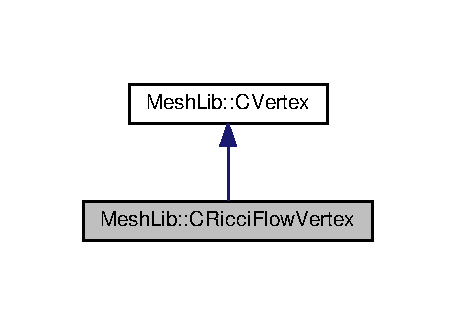
\includegraphics[width=219pt]{class_mesh_lib_1_1_c_ricci_flow_vertex__inherit__graph}
\end{center}
\end{figure}


Collaboration diagram for Mesh\+Lib\+:\+:C\+Ricci\+Flow\+Vertex\+:
\nopagebreak
\begin{figure}[H]
\begin{center}
\leavevmode
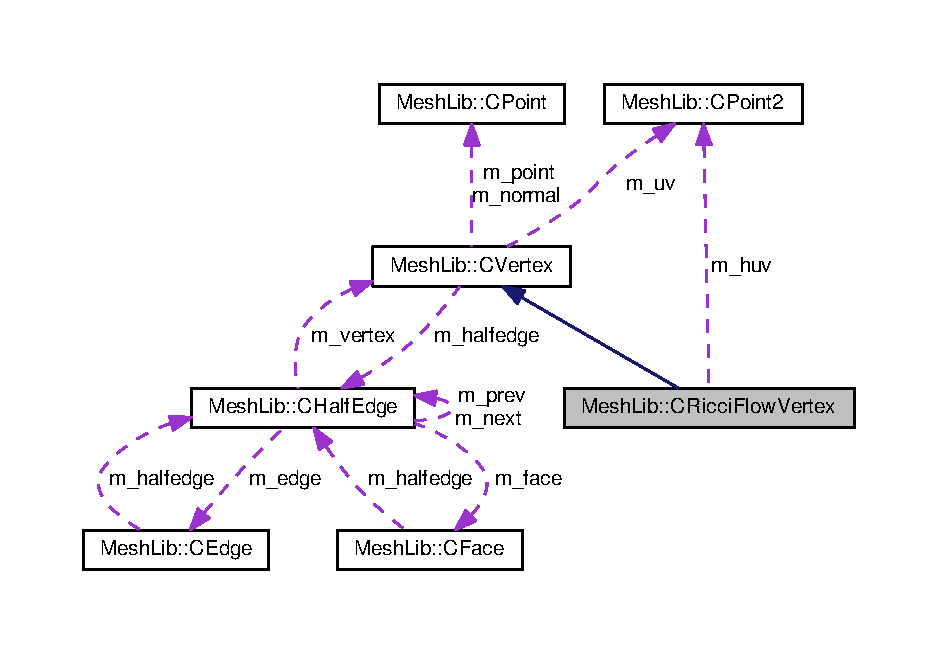
\includegraphics[width=350pt]{class_mesh_lib_1_1_c_ricci_flow_vertex__coll__graph}
\end{center}
\end{figure}
\subsection*{Public Member Functions}
\begin{DoxyCompactItemize}
\item 
\hyperlink{class_mesh_lib_1_1_c_ricci_flow_vertex_a5b32338308bba490c199901032b2bf4d}{C\+Ricci\+Flow\+Vertex} ()
\item 
\hyperlink{class_mesh_lib_1_1_c_ricci_flow_vertex_a42c6854f6acd34b70d14e588f5317f2a}{$\sim$\+C\+Ricci\+Flow\+Vertex} ()
\item 
\hyperlink{class_mesh_lib_1_1_c_point2}{C\+Point2} \& \hyperlink{class_mesh_lib_1_1_c_ricci_flow_vertex_aab160a0b027baa770beabe94a40158a1}{huv} ()
\item 
int \& \hyperlink{class_mesh_lib_1_1_c_ricci_flow_vertex_a6dc51d4254e173e2b98ebc4eee42a66c}{idx} ()
\item 
int \& \hyperlink{class_mesh_lib_1_1_c_ricci_flow_vertex_a03ba58a37f894d33544b5f5d1f37ba98}{father} ()
\item 
double \& \hyperlink{class_mesh_lib_1_1_c_ricci_flow_vertex_aa82637ce2940925c7dfdf26bb0e6c187}{u} ()
\item 
double \& \hyperlink{class_mesh_lib_1_1_c_ricci_flow_vertex_a3b5fff5cd648cd21846947857656ea7f}{k} ()
\item 
double \& \hyperlink{class_mesh_lib_1_1_c_ricci_flow_vertex_ab2edd249e38187bf0f12951077d088af}{target\+\_\+k} ()
\item 
bool \& \hyperlink{class_mesh_lib_1_1_c_ricci_flow_vertex_a2fa1403822fd623c1aafb33fbd8e3bac}{touched} ()
\item 
void \hyperlink{class_mesh_lib_1_1_c_ricci_flow_vertex_a769e46b30986e7942a2575f924013595}{\+\_\+from\+\_\+string} ()
\item 
void \hyperlink{class_mesh_lib_1_1_c_ricci_flow_vertex_a1d4ea035d20566e859dea5ae399f6b3a}{\+\_\+to\+\_\+string} ()
\item 
int \& \hyperlink{class_mesh_lib_1_1_c_ricci_flow_vertex_a21b0cb5288ee5b2b12d5a47c12b16d95}{valence} ()
\end{DoxyCompactItemize}
\subsection*{Static Public Attributes}
\begin{DoxyCompactItemize}
\item 
static unsigned int \hyperlink{class_mesh_lib_1_1_c_ricci_flow_vertex_a3af1d7b46bd87f486a1e6dbea027c91d}{traits}
\end{DoxyCompactItemize}
\subsection*{Protected Attributes}
\begin{DoxyCompactItemize}
\item 
\hyperlink{class_mesh_lib_1_1_c_point2}{C\+Point2} \hyperlink{class_mesh_lib_1_1_c_ricci_flow_vertex_a674116f5178c06d98b5ef26deabdeec6}{m\+\_\+huv}
\item 
int \hyperlink{class_mesh_lib_1_1_c_ricci_flow_vertex_a7ab6932d891ddbb10c14f0ab984d3b36}{m\+\_\+index}
\item 
int \hyperlink{class_mesh_lib_1_1_c_ricci_flow_vertex_a6ed5050df5a2f6284a98bb37c553a57e}{m\+\_\+father}
\item 
double \hyperlink{class_mesh_lib_1_1_c_ricci_flow_vertex_ac9f92366ddb0d823a6dfc6a526db9295}{m\+\_\+log\+\_\+radius}
\item 
double \hyperlink{class_mesh_lib_1_1_c_ricci_flow_vertex_a4b6a000486252eb17ece2e2ba4bc60a8}{m\+\_\+curvature}
\item 
double \hyperlink{class_mesh_lib_1_1_c_ricci_flow_vertex_abdfb30ac08fc9aff4c7052bfb4986de3}{m\+\_\+target\+\_\+curvature}
\item 
bool \hyperlink{class_mesh_lib_1_1_c_ricci_flow_vertex_ac66ef1157c3442bb632cdf89d509370e}{m\+\_\+touched}
\item 
int \hyperlink{class_mesh_lib_1_1_c_ricci_flow_vertex_a5a1d0671376b738ad92c860eeb24eb09}{m\+\_\+valence}
\end{DoxyCompactItemize}


\subsection{Detailed Description}
\hyperlink{class_mesh_lib_1_1_c_ricci_flow_vertex}{C\+Ricci\+Flow\+Vertex} class. 

Vertex class for Ricci flow Traits\+: index father log\+\_\+radius curvature vertex uv target\+\_\+curvature touched 

Definition at line 47 of file Ricci\+Flow\+Mesh.\+h.



\subsection{Constructor \& Destructor Documentation}
\index{Mesh\+Lib\+::\+C\+Ricci\+Flow\+Vertex@{Mesh\+Lib\+::\+C\+Ricci\+Flow\+Vertex}!C\+Ricci\+Flow\+Vertex@{C\+Ricci\+Flow\+Vertex}}
\index{C\+Ricci\+Flow\+Vertex@{C\+Ricci\+Flow\+Vertex}!Mesh\+Lib\+::\+C\+Ricci\+Flow\+Vertex@{Mesh\+Lib\+::\+C\+Ricci\+Flow\+Vertex}}
\subsubsection[{\texorpdfstring{C\+Ricci\+Flow\+Vertex()}{CRicciFlowVertex()}}]{\setlength{\rightskip}{0pt plus 5cm}Mesh\+Lib\+::\+C\+Ricci\+Flow\+Vertex\+::\+C\+Ricci\+Flow\+Vertex (
\begin{DoxyParamCaption}
{}
\end{DoxyParamCaption}
)\hspace{0.3cm}{\ttfamily [inline]}}\hypertarget{class_mesh_lib_1_1_c_ricci_flow_vertex_a5b32338308bba490c199901032b2bf4d}{}\label{class_mesh_lib_1_1_c_ricci_flow_vertex_a5b32338308bba490c199901032b2bf4d}
\hyperlink{class_mesh_lib_1_1_c_ricci_flow_vertex}{C\+Ricci\+Flow\+Vertex} constructor 

Definition at line 61 of file Ricci\+Flow\+Mesh.\+h.

\index{Mesh\+Lib\+::\+C\+Ricci\+Flow\+Vertex@{Mesh\+Lib\+::\+C\+Ricci\+Flow\+Vertex}!````~C\+Ricci\+Flow\+Vertex@{$\sim$\+C\+Ricci\+Flow\+Vertex}}
\index{````~C\+Ricci\+Flow\+Vertex@{$\sim$\+C\+Ricci\+Flow\+Vertex}!Mesh\+Lib\+::\+C\+Ricci\+Flow\+Vertex@{Mesh\+Lib\+::\+C\+Ricci\+Flow\+Vertex}}
\subsubsection[{\texorpdfstring{$\sim$\+C\+Ricci\+Flow\+Vertex()}{~CRicciFlowVertex()}}]{\setlength{\rightskip}{0pt plus 5cm}Mesh\+Lib\+::\+C\+Ricci\+Flow\+Vertex\+::$\sim$\+C\+Ricci\+Flow\+Vertex (
\begin{DoxyParamCaption}
{}
\end{DoxyParamCaption}
)\hspace{0.3cm}{\ttfamily [inline]}}\hypertarget{class_mesh_lib_1_1_c_ricci_flow_vertex_a42c6854f6acd34b70d14e588f5317f2a}{}\label{class_mesh_lib_1_1_c_ricci_flow_vertex_a42c6854f6acd34b70d14e588f5317f2a}
\hyperlink{class_mesh_lib_1_1_c_ricci_flow_vertex}{C\+Ricci\+Flow\+Vertex} destructor 

Definition at line 65 of file Ricci\+Flow\+Mesh.\+h.



\subsection{Member Function Documentation}
\index{Mesh\+Lib\+::\+C\+Ricci\+Flow\+Vertex@{Mesh\+Lib\+::\+C\+Ricci\+Flow\+Vertex}!\+\_\+from\+\_\+string@{\+\_\+from\+\_\+string}}
\index{\+\_\+from\+\_\+string@{\+\_\+from\+\_\+string}!Mesh\+Lib\+::\+C\+Ricci\+Flow\+Vertex@{Mesh\+Lib\+::\+C\+Ricci\+Flow\+Vertex}}
\subsubsection[{\texorpdfstring{\+\_\+from\+\_\+string()}{_from_string()}}]{\setlength{\rightskip}{0pt plus 5cm}void Mesh\+Lib\+::\+C\+Ricci\+Flow\+Vertex\+::\+\_\+from\+\_\+string (
\begin{DoxyParamCaption}
{}
\end{DoxyParamCaption}
)\hspace{0.3cm}{\ttfamily [inline]}}\hypertarget{class_mesh_lib_1_1_c_ricci_flow_vertex_a769e46b30986e7942a2575f924013595}{}\label{class_mesh_lib_1_1_c_ricci_flow_vertex_a769e46b30986e7942a2575f924013595}
Read vertex uv from vertex string 

Definition at line 135 of file Ricci\+Flow\+Mesh.\+h.

\index{Mesh\+Lib\+::\+C\+Ricci\+Flow\+Vertex@{Mesh\+Lib\+::\+C\+Ricci\+Flow\+Vertex}!\+\_\+to\+\_\+string@{\+\_\+to\+\_\+string}}
\index{\+\_\+to\+\_\+string@{\+\_\+to\+\_\+string}!Mesh\+Lib\+::\+C\+Ricci\+Flow\+Vertex@{Mesh\+Lib\+::\+C\+Ricci\+Flow\+Vertex}}
\subsubsection[{\texorpdfstring{\+\_\+to\+\_\+string()}{_to_string()}}]{\setlength{\rightskip}{0pt plus 5cm}void Mesh\+Lib\+::\+C\+Ricci\+Flow\+Vertex\+::\+\_\+to\+\_\+string (
\begin{DoxyParamCaption}
{}
\end{DoxyParamCaption}
)\hspace{0.3cm}{\ttfamily [inline]}}\hypertarget{class_mesh_lib_1_1_c_ricci_flow_vertex_a1d4ea035d20566e859dea5ae399f6b3a}{}\label{class_mesh_lib_1_1_c_ricci_flow_vertex_a1d4ea035d20566e859dea5ae399f6b3a}
Write vertex uv to vertex string 

Definition at line 170 of file Ricci\+Flow\+Mesh.\+h.

\index{Mesh\+Lib\+::\+C\+Ricci\+Flow\+Vertex@{Mesh\+Lib\+::\+C\+Ricci\+Flow\+Vertex}!father@{father}}
\index{father@{father}!Mesh\+Lib\+::\+C\+Ricci\+Flow\+Vertex@{Mesh\+Lib\+::\+C\+Ricci\+Flow\+Vertex}}
\subsubsection[{\texorpdfstring{father()}{father()}}]{\setlength{\rightskip}{0pt plus 5cm}int\& Mesh\+Lib\+::\+C\+Ricci\+Flow\+Vertex\+::father (
\begin{DoxyParamCaption}
{}
\end{DoxyParamCaption}
)\hspace{0.3cm}{\ttfamily [inline]}}\hypertarget{class_mesh_lib_1_1_c_ricci_flow_vertex_a03ba58a37f894d33544b5f5d1f37ba98}{}\label{class_mesh_lib_1_1_c_ricci_flow_vertex_a03ba58a37f894d33544b5f5d1f37ba98}
Vertex father trait 

Definition at line 78 of file Ricci\+Flow\+Mesh.\+h.

\index{Mesh\+Lib\+::\+C\+Ricci\+Flow\+Vertex@{Mesh\+Lib\+::\+C\+Ricci\+Flow\+Vertex}!huv@{huv}}
\index{huv@{huv}!Mesh\+Lib\+::\+C\+Ricci\+Flow\+Vertex@{Mesh\+Lib\+::\+C\+Ricci\+Flow\+Vertex}}
\subsubsection[{\texorpdfstring{huv()}{huv()}}]{\setlength{\rightskip}{0pt plus 5cm}{\bf C\+Point2}\& Mesh\+Lib\+::\+C\+Ricci\+Flow\+Vertex\+::huv (
\begin{DoxyParamCaption}
{}
\end{DoxyParamCaption}
)\hspace{0.3cm}{\ttfamily [inline]}}\hypertarget{class_mesh_lib_1_1_c_ricci_flow_vertex_aab160a0b027baa770beabe94a40158a1}{}\label{class_mesh_lib_1_1_c_ricci_flow_vertex_aab160a0b027baa770beabe94a40158a1}
Vertex uv trait 

Definition at line 70 of file Ricci\+Flow\+Mesh.\+h.

\index{Mesh\+Lib\+::\+C\+Ricci\+Flow\+Vertex@{Mesh\+Lib\+::\+C\+Ricci\+Flow\+Vertex}!idx@{idx}}
\index{idx@{idx}!Mesh\+Lib\+::\+C\+Ricci\+Flow\+Vertex@{Mesh\+Lib\+::\+C\+Ricci\+Flow\+Vertex}}
\subsubsection[{\texorpdfstring{idx()}{idx()}}]{\setlength{\rightskip}{0pt plus 5cm}int\& Mesh\+Lib\+::\+C\+Ricci\+Flow\+Vertex\+::idx (
\begin{DoxyParamCaption}
{}
\end{DoxyParamCaption}
)\hspace{0.3cm}{\ttfamily [inline]}}\hypertarget{class_mesh_lib_1_1_c_ricci_flow_vertex_a6dc51d4254e173e2b98ebc4eee42a66c}{}\label{class_mesh_lib_1_1_c_ricci_flow_vertex_a6dc51d4254e173e2b98ebc4eee42a66c}
Vertex index trait 

Definition at line 74 of file Ricci\+Flow\+Mesh.\+h.

\index{Mesh\+Lib\+::\+C\+Ricci\+Flow\+Vertex@{Mesh\+Lib\+::\+C\+Ricci\+Flow\+Vertex}!k@{k}}
\index{k@{k}!Mesh\+Lib\+::\+C\+Ricci\+Flow\+Vertex@{Mesh\+Lib\+::\+C\+Ricci\+Flow\+Vertex}}
\subsubsection[{\texorpdfstring{k()}{k()}}]{\setlength{\rightskip}{0pt plus 5cm}double\& Mesh\+Lib\+::\+C\+Ricci\+Flow\+Vertex\+::k (
\begin{DoxyParamCaption}
{}
\end{DoxyParamCaption}
)\hspace{0.3cm}{\ttfamily [inline]}}\hypertarget{class_mesh_lib_1_1_c_ricci_flow_vertex_a3b5fff5cd648cd21846947857656ea7f}{}\label{class_mesh_lib_1_1_c_ricci_flow_vertex_a3b5fff5cd648cd21846947857656ea7f}
Vertex curvature trait 

Definition at line 86 of file Ricci\+Flow\+Mesh.\+h.

\index{Mesh\+Lib\+::\+C\+Ricci\+Flow\+Vertex@{Mesh\+Lib\+::\+C\+Ricci\+Flow\+Vertex}!target\+\_\+k@{target\+\_\+k}}
\index{target\+\_\+k@{target\+\_\+k}!Mesh\+Lib\+::\+C\+Ricci\+Flow\+Vertex@{Mesh\+Lib\+::\+C\+Ricci\+Flow\+Vertex}}
\subsubsection[{\texorpdfstring{target\+\_\+k()}{target_k()}}]{\setlength{\rightskip}{0pt plus 5cm}double\& Mesh\+Lib\+::\+C\+Ricci\+Flow\+Vertex\+::target\+\_\+k (
\begin{DoxyParamCaption}
{}
\end{DoxyParamCaption}
)\hspace{0.3cm}{\ttfamily [inline]}}\hypertarget{class_mesh_lib_1_1_c_ricci_flow_vertex_ab2edd249e38187bf0f12951077d088af}{}\label{class_mesh_lib_1_1_c_ricci_flow_vertex_ab2edd249e38187bf0f12951077d088af}
Vertex target curvature 

Definition at line 90 of file Ricci\+Flow\+Mesh.\+h.

\index{Mesh\+Lib\+::\+C\+Ricci\+Flow\+Vertex@{Mesh\+Lib\+::\+C\+Ricci\+Flow\+Vertex}!touched@{touched}}
\index{touched@{touched}!Mesh\+Lib\+::\+C\+Ricci\+Flow\+Vertex@{Mesh\+Lib\+::\+C\+Ricci\+Flow\+Vertex}}
\subsubsection[{\texorpdfstring{touched()}{touched()}}]{\setlength{\rightskip}{0pt plus 5cm}bool\& Mesh\+Lib\+::\+C\+Ricci\+Flow\+Vertex\+::touched (
\begin{DoxyParamCaption}
{}
\end{DoxyParamCaption}
)\hspace{0.3cm}{\ttfamily [inline]}}\hypertarget{class_mesh_lib_1_1_c_ricci_flow_vertex_a2fa1403822fd623c1aafb33fbd8e3bac}{}\label{class_mesh_lib_1_1_c_ricci_flow_vertex_a2fa1403822fd623c1aafb33fbd8e3bac}
whether the vertex has been touched 

Definition at line 94 of file Ricci\+Flow\+Mesh.\+h.

\index{Mesh\+Lib\+::\+C\+Ricci\+Flow\+Vertex@{Mesh\+Lib\+::\+C\+Ricci\+Flow\+Vertex}!u@{u}}
\index{u@{u}!Mesh\+Lib\+::\+C\+Ricci\+Flow\+Vertex@{Mesh\+Lib\+::\+C\+Ricci\+Flow\+Vertex}}
\subsubsection[{\texorpdfstring{u()}{u()}}]{\setlength{\rightskip}{0pt plus 5cm}double\& Mesh\+Lib\+::\+C\+Ricci\+Flow\+Vertex\+::u (
\begin{DoxyParamCaption}
{}
\end{DoxyParamCaption}
)\hspace{0.3cm}{\ttfamily [inline]}}\hypertarget{class_mesh_lib_1_1_c_ricci_flow_vertex_aa82637ce2940925c7dfdf26bb0e6c187}{}\label{class_mesh_lib_1_1_c_ricci_flow_vertex_aa82637ce2940925c7dfdf26bb0e6c187}
Vertex log radius 

Definition at line 82 of file Ricci\+Flow\+Mesh.\+h.

\index{Mesh\+Lib\+::\+C\+Ricci\+Flow\+Vertex@{Mesh\+Lib\+::\+C\+Ricci\+Flow\+Vertex}!valence@{valence}}
\index{valence@{valence}!Mesh\+Lib\+::\+C\+Ricci\+Flow\+Vertex@{Mesh\+Lib\+::\+C\+Ricci\+Flow\+Vertex}}
\subsubsection[{\texorpdfstring{valence()}{valence()}}]{\setlength{\rightskip}{0pt plus 5cm}int\& Mesh\+Lib\+::\+C\+Ricci\+Flow\+Vertex\+::valence (
\begin{DoxyParamCaption}
{}
\end{DoxyParamCaption}
)\hspace{0.3cm}{\ttfamily [inline]}}\hypertarget{class_mesh_lib_1_1_c_ricci_flow_vertex_a21b0cb5288ee5b2b12d5a47c12b16d95}{}\label{class_mesh_lib_1_1_c_ricci_flow_vertex_a21b0cb5288ee5b2b12d5a47c12b16d95}
Topological valence of the vertex 

Definition at line 107 of file Ricci\+Flow\+Mesh.\+h.



\subsection{Member Data Documentation}
\index{Mesh\+Lib\+::\+C\+Ricci\+Flow\+Vertex@{Mesh\+Lib\+::\+C\+Ricci\+Flow\+Vertex}!m\+\_\+curvature@{m\+\_\+curvature}}
\index{m\+\_\+curvature@{m\+\_\+curvature}!Mesh\+Lib\+::\+C\+Ricci\+Flow\+Vertex@{Mesh\+Lib\+::\+C\+Ricci\+Flow\+Vertex}}
\subsubsection[{\texorpdfstring{m\+\_\+curvature}{m_curvature}}]{\setlength{\rightskip}{0pt plus 5cm}double Mesh\+Lib\+::\+C\+Ricci\+Flow\+Vertex\+::m\+\_\+curvature\hspace{0.3cm}{\ttfamily [protected]}}\hypertarget{class_mesh_lib_1_1_c_ricci_flow_vertex_a4b6a000486252eb17ece2e2ba4bc60a8}{}\label{class_mesh_lib_1_1_c_ricci_flow_vertex_a4b6a000486252eb17ece2e2ba4bc60a8}


Definition at line 123 of file Ricci\+Flow\+Mesh.\+h.

\index{Mesh\+Lib\+::\+C\+Ricci\+Flow\+Vertex@{Mesh\+Lib\+::\+C\+Ricci\+Flow\+Vertex}!m\+\_\+father@{m\+\_\+father}}
\index{m\+\_\+father@{m\+\_\+father}!Mesh\+Lib\+::\+C\+Ricci\+Flow\+Vertex@{Mesh\+Lib\+::\+C\+Ricci\+Flow\+Vertex}}
\subsubsection[{\texorpdfstring{m\+\_\+father}{m_father}}]{\setlength{\rightskip}{0pt plus 5cm}int Mesh\+Lib\+::\+C\+Ricci\+Flow\+Vertex\+::m\+\_\+father\hspace{0.3cm}{\ttfamily [protected]}}\hypertarget{class_mesh_lib_1_1_c_ricci_flow_vertex_a6ed5050df5a2f6284a98bb37c553a57e}{}\label{class_mesh_lib_1_1_c_ricci_flow_vertex_a6ed5050df5a2f6284a98bb37c553a57e}


Definition at line 119 of file Ricci\+Flow\+Mesh.\+h.

\index{Mesh\+Lib\+::\+C\+Ricci\+Flow\+Vertex@{Mesh\+Lib\+::\+C\+Ricci\+Flow\+Vertex}!m\+\_\+huv@{m\+\_\+huv}}
\index{m\+\_\+huv@{m\+\_\+huv}!Mesh\+Lib\+::\+C\+Ricci\+Flow\+Vertex@{Mesh\+Lib\+::\+C\+Ricci\+Flow\+Vertex}}
\subsubsection[{\texorpdfstring{m\+\_\+huv}{m_huv}}]{\setlength{\rightskip}{0pt plus 5cm}{\bf C\+Point2} Mesh\+Lib\+::\+C\+Ricci\+Flow\+Vertex\+::m\+\_\+huv\hspace{0.3cm}{\ttfamily [protected]}}\hypertarget{class_mesh_lib_1_1_c_ricci_flow_vertex_a674116f5178c06d98b5ef26deabdeec6}{}\label{class_mesh_lib_1_1_c_ricci_flow_vertex_a674116f5178c06d98b5ef26deabdeec6}
Vertex color

Vertex uv 

Definition at line 107 of file Ricci\+Flow\+Mesh.\+h.

\index{Mesh\+Lib\+::\+C\+Ricci\+Flow\+Vertex@{Mesh\+Lib\+::\+C\+Ricci\+Flow\+Vertex}!m\+\_\+index@{m\+\_\+index}}
\index{m\+\_\+index@{m\+\_\+index}!Mesh\+Lib\+::\+C\+Ricci\+Flow\+Vertex@{Mesh\+Lib\+::\+C\+Ricci\+Flow\+Vertex}}
\subsubsection[{\texorpdfstring{m\+\_\+index}{m_index}}]{\setlength{\rightskip}{0pt plus 5cm}int Mesh\+Lib\+::\+C\+Ricci\+Flow\+Vertex\+::m\+\_\+index\hspace{0.3cm}{\ttfamily [protected]}}\hypertarget{class_mesh_lib_1_1_c_ricci_flow_vertex_a7ab6932d891ddbb10c14f0ab984d3b36}{}\label{class_mesh_lib_1_1_c_ricci_flow_vertex_a7ab6932d891ddbb10c14f0ab984d3b36}
Vertex index 

Definition at line 117 of file Ricci\+Flow\+Mesh.\+h.

\index{Mesh\+Lib\+::\+C\+Ricci\+Flow\+Vertex@{Mesh\+Lib\+::\+C\+Ricci\+Flow\+Vertex}!m\+\_\+log\+\_\+radius@{m\+\_\+log\+\_\+radius}}
\index{m\+\_\+log\+\_\+radius@{m\+\_\+log\+\_\+radius}!Mesh\+Lib\+::\+C\+Ricci\+Flow\+Vertex@{Mesh\+Lib\+::\+C\+Ricci\+Flow\+Vertex}}
\subsubsection[{\texorpdfstring{m\+\_\+log\+\_\+radius}{m_log_radius}}]{\setlength{\rightskip}{0pt plus 5cm}double Mesh\+Lib\+::\+C\+Ricci\+Flow\+Vertex\+::m\+\_\+log\+\_\+radius\hspace{0.3cm}{\ttfamily [protected]}}\hypertarget{class_mesh_lib_1_1_c_ricci_flow_vertex_ac9f92366ddb0d823a6dfc6a526db9295}{}\label{class_mesh_lib_1_1_c_ricci_flow_vertex_ac9f92366ddb0d823a6dfc6a526db9295}


Definition at line 121 of file Ricci\+Flow\+Mesh.\+h.

\index{Mesh\+Lib\+::\+C\+Ricci\+Flow\+Vertex@{Mesh\+Lib\+::\+C\+Ricci\+Flow\+Vertex}!m\+\_\+target\+\_\+curvature@{m\+\_\+target\+\_\+curvature}}
\index{m\+\_\+target\+\_\+curvature@{m\+\_\+target\+\_\+curvature}!Mesh\+Lib\+::\+C\+Ricci\+Flow\+Vertex@{Mesh\+Lib\+::\+C\+Ricci\+Flow\+Vertex}}
\subsubsection[{\texorpdfstring{m\+\_\+target\+\_\+curvature}{m_target_curvature}}]{\setlength{\rightskip}{0pt plus 5cm}double Mesh\+Lib\+::\+C\+Ricci\+Flow\+Vertex\+::m\+\_\+target\+\_\+curvature\hspace{0.3cm}{\ttfamily [protected]}}\hypertarget{class_mesh_lib_1_1_c_ricci_flow_vertex_abdfb30ac08fc9aff4c7052bfb4986de3}{}\label{class_mesh_lib_1_1_c_ricci_flow_vertex_abdfb30ac08fc9aff4c7052bfb4986de3}


Definition at line 125 of file Ricci\+Flow\+Mesh.\+h.

\index{Mesh\+Lib\+::\+C\+Ricci\+Flow\+Vertex@{Mesh\+Lib\+::\+C\+Ricci\+Flow\+Vertex}!m\+\_\+touched@{m\+\_\+touched}}
\index{m\+\_\+touched@{m\+\_\+touched}!Mesh\+Lib\+::\+C\+Ricci\+Flow\+Vertex@{Mesh\+Lib\+::\+C\+Ricci\+Flow\+Vertex}}
\subsubsection[{\texorpdfstring{m\+\_\+touched}{m_touched}}]{\setlength{\rightskip}{0pt plus 5cm}bool Mesh\+Lib\+::\+C\+Ricci\+Flow\+Vertex\+::m\+\_\+touched\hspace{0.3cm}{\ttfamily [protected]}}\hypertarget{class_mesh_lib_1_1_c_ricci_flow_vertex_ac66ef1157c3442bb632cdf89d509370e}{}\label{class_mesh_lib_1_1_c_ricci_flow_vertex_ac66ef1157c3442bb632cdf89d509370e}


Definition at line 127 of file Ricci\+Flow\+Mesh.\+h.

\index{Mesh\+Lib\+::\+C\+Ricci\+Flow\+Vertex@{Mesh\+Lib\+::\+C\+Ricci\+Flow\+Vertex}!m\+\_\+valence@{m\+\_\+valence}}
\index{m\+\_\+valence@{m\+\_\+valence}!Mesh\+Lib\+::\+C\+Ricci\+Flow\+Vertex@{Mesh\+Lib\+::\+C\+Ricci\+Flow\+Vertex}}
\subsubsection[{\texorpdfstring{m\+\_\+valence}{m_valence}}]{\setlength{\rightskip}{0pt plus 5cm}int Mesh\+Lib\+::\+C\+Ricci\+Flow\+Vertex\+::m\+\_\+valence\hspace{0.3cm}{\ttfamily [protected]}}\hypertarget{class_mesh_lib_1_1_c_ricci_flow_vertex_a5a1d0671376b738ad92c860eeb24eb09}{}\label{class_mesh_lib_1_1_c_ricci_flow_vertex_a5a1d0671376b738ad92c860eeb24eb09}


Definition at line 129 of file Ricci\+Flow\+Mesh.\+h.

\index{Mesh\+Lib\+::\+C\+Ricci\+Flow\+Vertex@{Mesh\+Lib\+::\+C\+Ricci\+Flow\+Vertex}!traits@{traits}}
\index{traits@{traits}!Mesh\+Lib\+::\+C\+Ricci\+Flow\+Vertex@{Mesh\+Lib\+::\+C\+Ricci\+Flow\+Vertex}}
\subsubsection[{\texorpdfstring{traits}{traits}}]{\setlength{\rightskip}{0pt plus 5cm}unsigned int Mesh\+Lib\+::\+C\+Ricci\+Flow\+Vertex\+::traits\hspace{0.3cm}{\ttfamily [static]}}\hypertarget{class_mesh_lib_1_1_c_ricci_flow_vertex_a3af1d7b46bd87f486a1e6dbea027c91d}{}\label{class_mesh_lib_1_1_c_ricci_flow_vertex_a3af1d7b46bd87f486a1e6dbea027c91d}
Each bit in the traits indicates whether the vertex class has the correpsonding trait. e.\+g. if ( traits \& T\+R\+A\+I\+T\+\_\+\+UV ), then vertex-\/$>$\hyperlink{class_mesh_lib_1_1_c_ricci_flow_vertex_aab160a0b027baa770beabe94a40158a1}{huv()} needs to be stored int the vertex string. 

Definition at line 56 of file Ricci\+Flow\+Mesh.\+h.



The documentation for this class was generated from the following file\+:\begin{DoxyCompactItemize}
\item 
Mesh\+Lib/algorithm/\+Riemannian/\+Ricci\+Flow/\hyperlink{_ricci_flow_mesh_8h}{Ricci\+Flow\+Mesh.\+h}\end{DoxyCompactItemize}

\hypertarget{class_mesh_lib_1_1_c_structure}{}\section{Mesh\+Lib\+:\+:C\+Structure$<$ Mesh, V, E, F, H $>$ Class Template Reference}
\label{class_mesh_lib_1_1_c_structure}\index{Mesh\+Lib\+::\+C\+Structure$<$ Mesh, V, E, F, H $>$@{Mesh\+Lib\+::\+C\+Structure$<$ Mesh, V, E, F, H $>$}}


Conversion class.  




{\ttfamily \#include $<$Structure.\+h$>$}

\subsection*{Public Member Functions}
\begin{DoxyCompactItemize}
\item 
\hyperlink{class_mesh_lib_1_1_c_structure_a368f9061a7c92f3b85b9f59348b7f651}{C\+Structure} (Mesh $\ast$p\+Mesh)
\begin{DoxyCompactList}\small\item\em \hyperlink{class_mesh_lib_1_1_c_base_ricci_flow}{C\+Base\+Ricci\+Flow} constructor. \end{DoxyCompactList}\item 
\hyperlink{class_mesh_lib_1_1_c_structure_aef09abc61c919cf9c010497b6bad37cd}{$\sim$\+C\+Structure} ()
\begin{DoxyCompactList}\small\item\em \hyperlink{class_mesh_lib_1_1_c_base_ricci_flow}{C\+Base\+Ricci\+Flow} destructor. \end{DoxyCompactList}\item 
void \hyperlink{class_mesh_lib_1_1_c_structure_a9d4f67774556baf84aed076aab390ede}{\+\_\+metric\+\_\+2\+\_\+angle} ()
\item 
void \hyperlink{class_mesh_lib_1_1_c_structure_a10e9ac6f3e546003459d310df209bdd4}{\+\_\+embedding\+\_\+2\+\_\+metric} ()
\item 
void \hyperlink{class_mesh_lib_1_1_c_structure_aab9a90ee8e1f2a7b5bea24c0b070d239}{\+\_\+angle\+\_\+2\+\_\+curvature} ()
\item 
void \hyperlink{class_mesh_lib_1_1_c_structure_a1583325c9a7640865d6fe55556c070f3}{\+\_\+angle\+\_\+2\+\_\+\+Laplace} ()
\item 
void \hyperlink{class_mesh_lib_1_1_c_structure_a4855cc5a0ce8770288a38badca7c6b9d}{\+\_\+parameter\+\_\+mu\+\_\+2\+\_\+metric} ()
\item 
void \hyperlink{class_mesh_lib_1_1_c_structure_aba95682430a57dab163cf54424ab05da}{\+\_\+metric\+\_\+2\+\_\+diagonal\+\_\+ratio} ()
\item 
void \hyperlink{class_mesh_lib_1_1_c_structure_a5b329be24b5f12cc420fe9dd70270efc}{\+\_\+parameter\+\_\+mu\+\_\+2\+\_\+angle} ()
\end{DoxyCompactItemize}
\subsection*{Protected Member Functions}
\begin{DoxyCompactItemize}
\item 
double \hyperlink{class_mesh_lib_1_1_c_structure_a3cf9efb8667b631cdea313524d1f2517}{\+\_\+cosine\+\_\+law} (double a, double b, double c)
\item 
int \hyperlink{class_mesh_lib_1_1_c_structure_a7b6c7c5319e26dc4e418554e379fc973}{\+\_\+circle\+\_\+circle\+\_\+intersection} (double x0, double y0, double r0, double x1, double y1, double r1, double $\ast$xi, double $\ast$yi, double $\ast$xi\+\_\+prime, double $\ast$yi\+\_\+prime)
\item 
std\+::complex$<$ double $>$ \hyperlink{class_mesh_lib_1_1_c_structure_a0863a582fe471af9e19682e558c801be}{\+\_\+diagonal\+\_\+ratio} (Mesh $\ast$pM, E $\ast$pE)
\item 
bool \hyperlink{class_mesh_lib_1_1_c_structure_a04089c436e17ece0a1caba3aa167a111}{\+\_\+embed\+\_\+third\+\_\+vertex} (Mesh $\ast$pM, V $\ast$A, V $\ast$B, V $\ast$C)
\item 
void \hyperlink{class_mesh_lib_1_1_c_structure_a04bb3255b61df168864a13d952fbf65d}{\+\_\+embed\+\_\+two\+\_\+faces} (Mesh $\ast$PM, E $\ast$pE)
\item 
void \hyperlink{class_mesh_lib_1_1_c_structure_a2852dfc5fbd04e032b0a1542db48dad2}{\+\_\+embed\+\_\+one\+\_\+face} (Mesh $\ast$PM, E $\ast$pE)
\end{DoxyCompactItemize}
\subsection*{Protected Attributes}
\begin{DoxyCompactItemize}
\item 
Mesh $\ast$ \hyperlink{class_mesh_lib_1_1_c_structure_a9241359e43cc23ef2a70c9ada3bc73a7}{m\+\_\+p\+Mesh}
\end{DoxyCompactItemize}


\subsection{Detailed Description}
\subsubsection*{template$<$class Mesh, class V, class E, class F, class H$>$\\*
class Mesh\+Lib\+::\+C\+Structure$<$ Mesh, V, E, F, H $>$}

Conversion class. 

Algorithm for converting from one structure to another 

Definition at line 37 of file Structure.\+h.



\subsection{Constructor \& Destructor Documentation}
\index{Mesh\+Lib\+::\+C\+Structure@{Mesh\+Lib\+::\+C\+Structure}!C\+Structure@{C\+Structure}}
\index{C\+Structure@{C\+Structure}!Mesh\+Lib\+::\+C\+Structure@{Mesh\+Lib\+::\+C\+Structure}}
\subsubsection[{\texorpdfstring{C\+Structure(\+Mesh $\ast$p\+Mesh)}{CStructure(Mesh *pMesh)}}]{\setlength{\rightskip}{0pt plus 5cm}template$<$class Mesh , class V , class E , class F , class H $>$ {\bf Mesh\+Lib\+::\+C\+Structure}$<$ Mesh, V, E, F, H $>$\+::{\bf C\+Structure} (
\begin{DoxyParamCaption}
\item[{Mesh $\ast$}]{p\+Mesh}
\end{DoxyParamCaption}
)\hspace{0.3cm}{\ttfamily [inline]}}\hypertarget{class_mesh_lib_1_1_c_structure_a368f9061a7c92f3b85b9f59348b7f651}{}\label{class_mesh_lib_1_1_c_structure_a368f9061a7c92f3b85b9f59348b7f651}


\hyperlink{class_mesh_lib_1_1_c_base_ricci_flow}{C\+Base\+Ricci\+Flow} constructor. 


\begin{DoxyParams}{Parameters}
{\em p\+Mesh} & the input mesh \\
\hline
\end{DoxyParams}


Definition at line 44 of file Structure.\+h.

\index{Mesh\+Lib\+::\+C\+Structure@{Mesh\+Lib\+::\+C\+Structure}!````~C\+Structure@{$\sim$\+C\+Structure}}
\index{````~C\+Structure@{$\sim$\+C\+Structure}!Mesh\+Lib\+::\+C\+Structure@{Mesh\+Lib\+::\+C\+Structure}}
\subsubsection[{\texorpdfstring{$\sim$\+C\+Structure()}{~CStructure()}}]{\setlength{\rightskip}{0pt plus 5cm}template$<$class Mesh , class V , class E , class F , class H $>$ {\bf Mesh\+Lib\+::\+C\+Structure}$<$ Mesh, V, E, F, H $>$\+::$\sim${\bf C\+Structure} (
\begin{DoxyParamCaption}
{}
\end{DoxyParamCaption}
)\hspace{0.3cm}{\ttfamily [inline]}}\hypertarget{class_mesh_lib_1_1_c_structure_aef09abc61c919cf9c010497b6bad37cd}{}\label{class_mesh_lib_1_1_c_structure_aef09abc61c919cf9c010497b6bad37cd}


\hyperlink{class_mesh_lib_1_1_c_base_ricci_flow}{C\+Base\+Ricci\+Flow} destructor. 



Definition at line 47 of file Structure.\+h.



\subsection{Member Function Documentation}
\index{Mesh\+Lib\+::\+C\+Structure@{Mesh\+Lib\+::\+C\+Structure}!\+\_\+angle\+\_\+2\+\_\+curvature@{\+\_\+angle\+\_\+2\+\_\+curvature}}
\index{\+\_\+angle\+\_\+2\+\_\+curvature@{\+\_\+angle\+\_\+2\+\_\+curvature}!Mesh\+Lib\+::\+C\+Structure@{Mesh\+Lib\+::\+C\+Structure}}
\subsubsection[{\texorpdfstring{\+\_\+angle\+\_\+2\+\_\+curvature()}{_angle_2_curvature()}}]{\setlength{\rightskip}{0pt plus 5cm}template$<$class M , class V , class E , class F , class H $>$ void {\bf Mesh\+Lib\+::\+C\+Structure}$<$ M, V, E, F, H $>$\+::\+\_\+angle\+\_\+2\+\_\+curvature (
\begin{DoxyParamCaption}
{}
\end{DoxyParamCaption}
)}\hypertarget{class_mesh_lib_1_1_c_structure_aab9a90ee8e1f2a7b5bea24c0b070d239}{}\label{class_mesh_lib_1_1_c_structure_aab9a90ee8e1f2a7b5bea24c0b070d239}
Convert angle structure to vertex curvature function 

Definition at line 208 of file Structure.\+h.

\index{Mesh\+Lib\+::\+C\+Structure@{Mesh\+Lib\+::\+C\+Structure}!\+\_\+angle\+\_\+2\+\_\+\+Laplace@{\+\_\+angle\+\_\+2\+\_\+\+Laplace}}
\index{\+\_\+angle\+\_\+2\+\_\+\+Laplace@{\+\_\+angle\+\_\+2\+\_\+\+Laplace}!Mesh\+Lib\+::\+C\+Structure@{Mesh\+Lib\+::\+C\+Structure}}
\subsubsection[{\texorpdfstring{\+\_\+angle\+\_\+2\+\_\+\+Laplace()}{_angle_2_Laplace()}}]{\setlength{\rightskip}{0pt plus 5cm}template$<$class M , class V , class E , class F , class H $>$ void {\bf Mesh\+Lib\+::\+C\+Structure}$<$ M, V, E, F, H $>$\+::\+\_\+angle\+\_\+2\+\_\+\+Laplace (
\begin{DoxyParamCaption}
{}
\end{DoxyParamCaption}
)}\hypertarget{class_mesh_lib_1_1_c_structure_a1583325c9a7640865d6fe55556c070f3}{}\label{class_mesh_lib_1_1_c_structure_a1583325c9a7640865d6fe55556c070f3}
Compute Laplace-\/\+Beltrami operator from angle structure

Compute the edge weight $ w(e) = \cot \alpha + \cot \beta $ where $\alpha,\beta$ are the two corner angles against edge $e$. $ w(e) = \cot \alpha $ If the edge is on the boundary, then 

Definition at line 229 of file Structure.\+h.

\index{Mesh\+Lib\+::\+C\+Structure@{Mesh\+Lib\+::\+C\+Structure}!\+\_\+circle\+\_\+circle\+\_\+intersection@{\+\_\+circle\+\_\+circle\+\_\+intersection}}
\index{\+\_\+circle\+\_\+circle\+\_\+intersection@{\+\_\+circle\+\_\+circle\+\_\+intersection}!Mesh\+Lib\+::\+C\+Structure@{Mesh\+Lib\+::\+C\+Structure}}
\subsubsection[{\texorpdfstring{\+\_\+circle\+\_\+circle\+\_\+intersection(double x0, double y0, double r0, double x1, double y1, double r1, double $\ast$xi, double $\ast$yi, double $\ast$xi\+\_\+prime, double $\ast$yi\+\_\+prime)}{_circle_circle_intersection(double x0, double y0, double r0, double x1, double y1, double r1, double *xi, double *yi, double *xi_prime, double *yi_prime)}}]{\setlength{\rightskip}{0pt plus 5cm}template$<$class M , class V , class E , class F , class H $>$ int {\bf Mesh\+Lib\+::\+C\+Structure}$<$ M, V, E, F, H $>$\+::\+\_\+circle\+\_\+circle\+\_\+intersection (
\begin{DoxyParamCaption}
\item[{double}]{x0, }
\item[{double}]{y0, }
\item[{double}]{r0, }
\item[{double}]{x1, }
\item[{double}]{y1, }
\item[{double}]{r1, }
\item[{double $\ast$}]{xi, }
\item[{double $\ast$}]{yi, }
\item[{double $\ast$}]{xi\+\_\+prime, }
\item[{double $\ast$}]{yi\+\_\+prime}
\end{DoxyParamCaption}
)\hspace{0.3cm}{\ttfamily [protected]}}\hypertarget{class_mesh_lib_1_1_c_structure_a7b6c7c5319e26dc4e418554e379fc973}{}\label{class_mesh_lib_1_1_c_structure_a7b6c7c5319e26dc4e418554e379fc973}
Compute the intersections of two circles 
\begin{DoxyParams}{Parameters}
{\em x0,y0,r1,x1,y1,r1} & are circles ( (x0,y0), r0 ) and ( (x1,y1), r1 ) \\
\hline
{\em xi,yi,xi\+\_\+prime,yi\+\_\+prime} & are the two intersection points \\
\hline
\end{DoxyParams}


Definition at line 305 of file Structure.\+h.

\index{Mesh\+Lib\+::\+C\+Structure@{Mesh\+Lib\+::\+C\+Structure}!\+\_\+cosine\+\_\+law@{\+\_\+cosine\+\_\+law}}
\index{\+\_\+cosine\+\_\+law@{\+\_\+cosine\+\_\+law}!Mesh\+Lib\+::\+C\+Structure@{Mesh\+Lib\+::\+C\+Structure}}
\subsubsection[{\texorpdfstring{\+\_\+cosine\+\_\+law(double a, double b, double c)}{_cosine_law(double a, double b, double c)}}]{\setlength{\rightskip}{0pt plus 5cm}template$<$class M , class V , class E , class F , class H $>$ double {\bf Mesh\+Lib\+::\+C\+Structure}$<$ M, V, E, F, H $>$\+::\+\_\+cosine\+\_\+law (
\begin{DoxyParamCaption}
\item[{double}]{a, }
\item[{double}]{b, }
\item[{double}]{c}
\end{DoxyParamCaption}
)\hspace{0.3cm}{\ttfamily [protected]}}\hypertarget{class_mesh_lib_1_1_c_structure_a3cf9efb8667b631cdea313524d1f2517}{}\label{class_mesh_lib_1_1_c_structure_a3cf9efb8667b631cdea313524d1f2517}
Euclidean Cosine law


\begin{DoxyParams}{Parameters}
{\em a,b,c} & edge lengths return angle C \\
\hline
\end{DoxyParams}


Definition at line 148 of file Structure.\+h.

\index{Mesh\+Lib\+::\+C\+Structure@{Mesh\+Lib\+::\+C\+Structure}!\+\_\+diagonal\+\_\+ratio@{\+\_\+diagonal\+\_\+ratio}}
\index{\+\_\+diagonal\+\_\+ratio@{\+\_\+diagonal\+\_\+ratio}!Mesh\+Lib\+::\+C\+Structure@{Mesh\+Lib\+::\+C\+Structure}}
\subsubsection[{\texorpdfstring{\+\_\+diagonal\+\_\+ratio(\+Mesh $\ast$p\+M, E $\ast$p\+E)}{_diagonal_ratio(Mesh *pM, E *pE)}}]{\setlength{\rightskip}{0pt plus 5cm}template$<$class Mesh , class V , class E , class F , class H $>$ std\+::complex$<$ double $>$ {\bf Mesh\+Lib\+::\+C\+Structure}$<$ M, V, E, F, H $>$\+::\+\_\+diagonal\+\_\+ratio (
\begin{DoxyParamCaption}
\item[{Mesh $\ast$}]{pM, }
\item[{E $\ast$}]{pE}
\end{DoxyParamCaption}
)\hspace{0.3cm}{\ttfamily [protected]}}\hypertarget{class_mesh_lib_1_1_c_structure_a0863a582fe471af9e19682e558c801be}{}\label{class_mesh_lib_1_1_c_structure_a0863a582fe471af9e19682e558c801be}
Compute the diagonal ratio on edge pE of mesh pM 
\begin{DoxyParams}{Parameters}
{\em pM} & input mesh, pE input edge  the diagonal ratio of the edge \\
\hline
\end{DoxyParams}


Definition at line 452 of file Structure.\+h.

\index{Mesh\+Lib\+::\+C\+Structure@{Mesh\+Lib\+::\+C\+Structure}!\+\_\+embed\+\_\+one\+\_\+face@{\+\_\+embed\+\_\+one\+\_\+face}}
\index{\+\_\+embed\+\_\+one\+\_\+face@{\+\_\+embed\+\_\+one\+\_\+face}!Mesh\+Lib\+::\+C\+Structure@{Mesh\+Lib\+::\+C\+Structure}}
\subsubsection[{\texorpdfstring{\+\_\+embed\+\_\+one\+\_\+face(\+Mesh $\ast$\+P\+M, E $\ast$p\+E)}{_embed_one_face(Mesh *PM, E *pE)}}]{\setlength{\rightskip}{0pt plus 5cm}template$<$class Mesh , class V , class E , class F , class H $>$ void {\bf Mesh\+Lib\+::\+C\+Structure}$<$ M, V, E, F, H $>$\+::\+\_\+embed\+\_\+one\+\_\+face (
\begin{DoxyParamCaption}
\item[{Mesh $\ast$}]{PM, }
\item[{E $\ast$}]{pE}
\end{DoxyParamCaption}
)\hspace{0.3cm}{\ttfamily [protected]}}\hypertarget{class_mesh_lib_1_1_c_structure_a2852dfc5fbd04e032b0a1542db48dad2}{}\label{class_mesh_lib_1_1_c_structure_a2852dfc5fbd04e032b0a1542db48dad2}
Isometrically embed the face adjacent to a boundary edge pE 
\begin{DoxyParams}{Parameters}
{\em pM} & input mesh, \\
\hline
{\em pE} & input edge, \\
\hline
\end{DoxyParams}


Definition at line 435 of file Structure.\+h.

\index{Mesh\+Lib\+::\+C\+Structure@{Mesh\+Lib\+::\+C\+Structure}!\+\_\+embed\+\_\+third\+\_\+vertex@{\+\_\+embed\+\_\+third\+\_\+vertex}}
\index{\+\_\+embed\+\_\+third\+\_\+vertex@{\+\_\+embed\+\_\+third\+\_\+vertex}!Mesh\+Lib\+::\+C\+Structure@{Mesh\+Lib\+::\+C\+Structure}}
\subsubsection[{\texorpdfstring{\+\_\+embed\+\_\+third\+\_\+vertex(\+Mesh $\ast$p\+M, V $\ast$\+A, V $\ast$\+B, V $\ast$\+C)}{_embed_third_vertex(Mesh *pM, V *A, V *B, V *C)}}]{\setlength{\rightskip}{0pt plus 5cm}template$<$class Mesh , class V , class E , class F , class H $>$ bool {\bf Mesh\+Lib\+::\+C\+Structure}$<$ M, V, E, F, H $>$\+::\+\_\+embed\+\_\+third\+\_\+vertex (
\begin{DoxyParamCaption}
\item[{Mesh $\ast$}]{pM, }
\item[{V $\ast$}]{A, }
\item[{V $\ast$}]{B, }
\item[{V $\ast$}]{C}
\end{DoxyParamCaption}
)\hspace{0.3cm}{\ttfamily [protected]}}\hypertarget{class_mesh_lib_1_1_c_structure_a04089c436e17ece0a1caba3aa167a111}{}\label{class_mesh_lib_1_1_c_structure_a04089c436e17ece0a1caba3aa167a111}
Vertex A, B, C are three vertices of a triangle, sorted C\+C\+Wly A and B have been embedded on the plane, isometrically embed vertex C 

Definition at line 371 of file Structure.\+h.

\index{Mesh\+Lib\+::\+C\+Structure@{Mesh\+Lib\+::\+C\+Structure}!\+\_\+embed\+\_\+two\+\_\+faces@{\+\_\+embed\+\_\+two\+\_\+faces}}
\index{\+\_\+embed\+\_\+two\+\_\+faces@{\+\_\+embed\+\_\+two\+\_\+faces}!Mesh\+Lib\+::\+C\+Structure@{Mesh\+Lib\+::\+C\+Structure}}
\subsubsection[{\texorpdfstring{\+\_\+embed\+\_\+two\+\_\+faces(\+Mesh $\ast$\+P\+M, E $\ast$p\+E)}{_embed_two_faces(Mesh *PM, E *pE)}}]{\setlength{\rightskip}{0pt plus 5cm}template$<$class Mesh , class V , class E , class F , class H $>$ void {\bf Mesh\+Lib\+::\+C\+Structure}$<$ M, V, E, F, H $>$\+::\+\_\+embed\+\_\+two\+\_\+faces (
\begin{DoxyParamCaption}
\item[{Mesh $\ast$}]{PM, }
\item[{E $\ast$}]{pE}
\end{DoxyParamCaption}
)\hspace{0.3cm}{\ttfamily [protected]}}\hypertarget{class_mesh_lib_1_1_c_structure_a04bb3255b61df168864a13d952fbf65d}{}\label{class_mesh_lib_1_1_c_structure_a04bb3255b61df168864a13d952fbf65d}
Isometrically embed two faces adjacent to an edge pE 
\begin{DoxyParams}{Parameters}
{\em pM} & input mesh, \\
\hline
{\em pE} & input edge, \\
\hline
\end{DoxyParams}


Definition at line 415 of file Structure.\+h.

\index{Mesh\+Lib\+::\+C\+Structure@{Mesh\+Lib\+::\+C\+Structure}!\+\_\+embedding\+\_\+2\+\_\+metric@{\+\_\+embedding\+\_\+2\+\_\+metric}}
\index{\+\_\+embedding\+\_\+2\+\_\+metric@{\+\_\+embedding\+\_\+2\+\_\+metric}!Mesh\+Lib\+::\+C\+Structure@{Mesh\+Lib\+::\+C\+Structure}}
\subsubsection[{\texorpdfstring{\+\_\+embedding\+\_\+2\+\_\+metric()}{_embedding_2_metric()}}]{\setlength{\rightskip}{0pt plus 5cm}template$<$class M , class V , class E , class F , class H $>$ void {\bf Mesh\+Lib\+::\+C\+Structure}$<$ M, V, E, F, H $>$\+::\+\_\+embedding\+\_\+2\+\_\+metric (
\begin{DoxyParamCaption}
{}
\end{DoxyParamCaption}
)}\hypertarget{class_mesh_lib_1_1_c_structure_a10e9ac6f3e546003459d310df209bdd4}{}\label{class_mesh_lib_1_1_c_structure_a10e9ac6f3e546003459d310df209bdd4}
Convert the embedding structure in R3 to metric structure 

Definition at line 191 of file Structure.\+h.

\index{Mesh\+Lib\+::\+C\+Structure@{Mesh\+Lib\+::\+C\+Structure}!\+\_\+metric\+\_\+2\+\_\+angle@{\+\_\+metric\+\_\+2\+\_\+angle}}
\index{\+\_\+metric\+\_\+2\+\_\+angle@{\+\_\+metric\+\_\+2\+\_\+angle}!Mesh\+Lib\+::\+C\+Structure@{Mesh\+Lib\+::\+C\+Structure}}
\subsubsection[{\texorpdfstring{\+\_\+metric\+\_\+2\+\_\+angle()}{_metric_2_angle()}}]{\setlength{\rightskip}{0pt plus 5cm}template$<$class M , class V , class E , class F , class H $>$ void {\bf Mesh\+Lib\+::\+C\+Structure}$<$ M, V, E, F, H $>$\+::\+\_\+metric\+\_\+2\+\_\+angle (
\begin{DoxyParamCaption}
{}
\end{DoxyParamCaption}
)}\hypertarget{class_mesh_lib_1_1_c_structure_a9d4f67774556baf84aed076aab390ede}{}\label{class_mesh_lib_1_1_c_structure_a9d4f67774556baf84aed076aab390ede}
Convert the metric structure to angle structure 

Definition at line 159 of file Structure.\+h.

\index{Mesh\+Lib\+::\+C\+Structure@{Mesh\+Lib\+::\+C\+Structure}!\+\_\+metric\+\_\+2\+\_\+diagonal\+\_\+ratio@{\+\_\+metric\+\_\+2\+\_\+diagonal\+\_\+ratio}}
\index{\+\_\+metric\+\_\+2\+\_\+diagonal\+\_\+ratio@{\+\_\+metric\+\_\+2\+\_\+diagonal\+\_\+ratio}!Mesh\+Lib\+::\+C\+Structure@{Mesh\+Lib\+::\+C\+Structure}}
\subsubsection[{\texorpdfstring{\+\_\+metric\+\_\+2\+\_\+diagonal\+\_\+ratio()}{_metric_2_diagonal_ratio()}}]{\setlength{\rightskip}{0pt plus 5cm}template$<$class M , class V , class E , class F , class H $>$ void {\bf Mesh\+Lib\+::\+C\+Structure}$<$ M, V, E, F, H $>$\+::\+\_\+metric\+\_\+2\+\_\+diagonal\+\_\+ratio (
\begin{DoxyParamCaption}
{}
\end{DoxyParamCaption}
)}\hypertarget{class_mesh_lib_1_1_c_structure_aba95682430a57dab163cf54424ab05da}{}\label{class_mesh_lib_1_1_c_structure_aba95682430a57dab163cf54424ab05da}
From Riemannian metric to compute the edge diagonal ratio Edge diagonal ratio is another way of representing conformal structure 

Definition at line 503 of file Structure.\+h.

\index{Mesh\+Lib\+::\+C\+Structure@{Mesh\+Lib\+::\+C\+Structure}!\+\_\+parameter\+\_\+mu\+\_\+2\+\_\+angle@{\+\_\+parameter\+\_\+mu\+\_\+2\+\_\+angle}}
\index{\+\_\+parameter\+\_\+mu\+\_\+2\+\_\+angle@{\+\_\+parameter\+\_\+mu\+\_\+2\+\_\+angle}!Mesh\+Lib\+::\+C\+Structure@{Mesh\+Lib\+::\+C\+Structure}}
\subsubsection[{\texorpdfstring{\+\_\+parameter\+\_\+mu\+\_\+2\+\_\+angle()}{_parameter_mu_2_angle()}}]{\setlength{\rightskip}{0pt plus 5cm}template$<$class M , class V , class E , class F , class H $>$ void {\bf Mesh\+Lib\+::\+C\+Structure}$<$ M, V, E, F, H $>$\+::\+\_\+parameter\+\_\+mu\+\_\+2\+\_\+angle (
\begin{DoxyParamCaption}
{}
\end{DoxyParamCaption}
)}\hypertarget{class_mesh_lib_1_1_c_structure_a5b329be24b5f12cc420fe9dd70270efc}{}\label{class_mesh_lib_1_1_c_structure_a5b329be24b5f12cc420fe9dd70270efc}
Conformal parameteriztion is set (vertex-\/$>$z()), Face Beltrami coefficient is set (face-\/$>$mu()), Compute the deformed angle structure 

Definition at line 517 of file Structure.\+h.

\index{Mesh\+Lib\+::\+C\+Structure@{Mesh\+Lib\+::\+C\+Structure}!\+\_\+parameter\+\_\+mu\+\_\+2\+\_\+metric@{\+\_\+parameter\+\_\+mu\+\_\+2\+\_\+metric}}
\index{\+\_\+parameter\+\_\+mu\+\_\+2\+\_\+metric@{\+\_\+parameter\+\_\+mu\+\_\+2\+\_\+metric}!Mesh\+Lib\+::\+C\+Structure@{Mesh\+Lib\+::\+C\+Structure}}
\subsubsection[{\texorpdfstring{\+\_\+parameter\+\_\+mu\+\_\+2\+\_\+metric()}{_parameter_mu_2_metric()}}]{\setlength{\rightskip}{0pt plus 5cm}template$<$class M , class V , class E , class F , class H $>$ void {\bf Mesh\+Lib\+::\+C\+Structure}$<$ M, V, E, F, H $>$\+::\+\_\+parameter\+\_\+mu\+\_\+2\+\_\+metric (
\begin{DoxyParamCaption}
{}
\end{DoxyParamCaption}
)}\hypertarget{class_mesh_lib_1_1_c_structure_a4855cc5a0ce8770288a38badca7c6b9d}{}\label{class_mesh_lib_1_1_c_structure_a4855cc5a0ce8770288a38badca7c6b9d}
Deform the angle structure by Beltrami coefficient

Conformal parameteriztion is set (vertex-\/$>$uv()), Vertex Beltrami coefficient is set (vertex-\/$>$mu()), Compute the deformed metric 

Definition at line 254 of file Structure.\+h.



\subsection{Member Data Documentation}
\index{Mesh\+Lib\+::\+C\+Structure@{Mesh\+Lib\+::\+C\+Structure}!m\+\_\+p\+Mesh@{m\+\_\+p\+Mesh}}
\index{m\+\_\+p\+Mesh@{m\+\_\+p\+Mesh}!Mesh\+Lib\+::\+C\+Structure@{Mesh\+Lib\+::\+C\+Structure}}
\subsubsection[{\texorpdfstring{m\+\_\+p\+Mesh}{m_pMesh}}]{\setlength{\rightskip}{0pt plus 5cm}template$<$class Mesh , class V , class E , class F , class H $>$ Mesh$\ast$ {\bf Mesh\+Lib\+::\+C\+Structure}$<$ Mesh, V, E, F, H $>$\+::m\+\_\+p\+Mesh\hspace{0.3cm}{\ttfamily [protected]}}\hypertarget{class_mesh_lib_1_1_c_structure_a9241359e43cc23ef2a70c9ada3bc73a7}{}\label{class_mesh_lib_1_1_c_structure_a9241359e43cc23ef2a70c9ada3bc73a7}
the input mesh 

Definition at line 99 of file Structure.\+h.



The documentation for this class was generated from the following file\+:\begin{DoxyCompactItemize}
\item 
Mesh\+Lib/algorithm/\+Structure/\hyperlink{_structure_8h}{Structure.\+h}\end{DoxyCompactItemize}

\hypertarget{class_mesh_lib_1_1_c_tangential_ricci_flow}{}\section{Mesh\+Lib\+:\+:C\+Tangential\+Ricci\+Flow$<$ V, E, F, H $>$ Class Template Reference}
\label{class_mesh_lib_1_1_c_tangential_ricci_flow}\index{Mesh\+Lib\+::\+C\+Tangential\+Ricci\+Flow$<$ V, E, F, H $>$@{Mesh\+Lib\+::\+C\+Tangential\+Ricci\+Flow$<$ V, E, F, H $>$}}


Class \hyperlink{class_mesh_lib_1_1_c_tangential_ricci_flow}{C\+Tangential\+Ricci\+Flow}.  




{\ttfamily \#include $<$Tangential\+Ricci\+Flow.\+h$>$}



Inheritance diagram for Mesh\+Lib\+:\+:C\+Tangential\+Ricci\+Flow$<$ V, E, F, H $>$\+:
\nopagebreak
\begin{figure}[H]
\begin{center}
\leavevmode
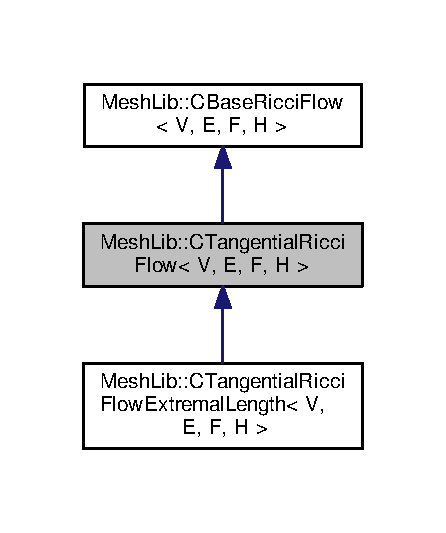
\includegraphics[width=214pt]{class_mesh_lib_1_1_c_tangential_ricci_flow__inherit__graph}
\end{center}
\end{figure}


Collaboration diagram for Mesh\+Lib\+:\+:C\+Tangential\+Ricci\+Flow$<$ V, E, F, H $>$\+:
\nopagebreak
\begin{figure}[H]
\begin{center}
\leavevmode
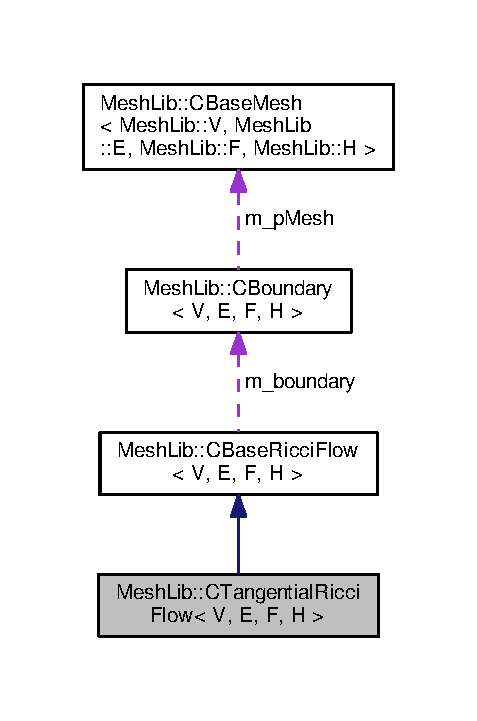
\includegraphics[width=229pt]{class_mesh_lib_1_1_c_tangential_ricci_flow__coll__graph}
\end{center}
\end{figure}
\subsection*{Public Member Functions}
\begin{DoxyCompactItemize}
\item 
\hyperlink{class_mesh_lib_1_1_c_tangential_ricci_flow_acf2f58bd7f00038259518d7fa1e4dfbf}{C\+Tangential\+Ricci\+Flow} (C\+Ricci\+Flow\+Mesh$<$ V, E, F, H $>$ $\ast$p\+Mesh)
\begin{DoxyCompactList}\small\item\em \hyperlink{class_mesh_lib_1_1_c_tangential_ricci_flow}{C\+Tangential\+Ricci\+Flow} constructor. \end{DoxyCompactList}\item 
\hyperlink{class_mesh_lib_1_1_c_tangential_ricci_flow_a4e7d0a53f0f06e93ae7af4da5d23aeec}{$\sim$\+C\+Tangential\+Ricci\+Flow} ()
\begin{DoxyCompactList}\small\item\em \hyperlink{class_mesh_lib_1_1_c_tangential_ricci_flow}{C\+Tangential\+Ricci\+Flow} destructor. \end{DoxyCompactList}\item 
void \hyperlink{class_mesh_lib_1_1_c_tangential_ricci_flow_a14983a8b8819f1b37a88bed0db5d1e4a}{\+\_\+calculate\+\_\+metric} ()
\item 
bool \hyperlink{class_mesh_lib_1_1_c_tangential_ricci_flow_a5ab0113d3d85597f6a782d8ca972bad7}{\+\_\+flow} (double)
\end{DoxyCompactItemize}
\subsection*{Protected Member Functions}
\begin{DoxyCompactItemize}
\item 
void \hyperlink{class_mesh_lib_1_1_c_tangential_ricci_flow_a902998c914ca63c77985daeda0a1cddd}{\+\_\+length} (double u1, double u2, E $\ast$e)
\item 
double \hyperlink{class_mesh_lib_1_1_c_tangential_ricci_flow_a5e066ca345120f963a6b859fbb0ac5d8}{\+\_\+cosine\+\_\+law} (double a, double b, double c)
\item 
void \hyperlink{class_mesh_lib_1_1_c_tangential_ricci_flow_a99223f86b1f13d3974c54ce319c212fe}{\+\_\+normalization} (Eigen\+::\+Vector\+Xd \&du, int n)
\item 
void \hyperlink{class_mesh_lib_1_1_c_tangential_ricci_flow_a94dde69c540846106ee0daa7d840e9cb}{\+\_\+calculate\+\_\+edge\+\_\+weight} ()
\item 
virtual void \hyperlink{class_mesh_lib_1_1_c_tangential_ricci_flow_ab7cbb76f7ca0de62311bc9c0cfc281e5}{\+\_\+set\+\_\+target\+\_\+curvature} ()
\end{DoxyCompactItemize}
\subsection*{Additional Inherited Members}


\subsection{Detailed Description}
\subsubsection*{template$<$class V, class E, class F, class H$>$\\*
class Mesh\+Lib\+::\+C\+Tangential\+Ricci\+Flow$<$ V, E, F, H $>$}

Class \hyperlink{class_mesh_lib_1_1_c_tangential_ricci_flow}{C\+Tangential\+Ricci\+Flow}. 

Algorithm for computing Ricci flow 

Definition at line 39 of file Tangential\+Ricci\+Flow.\+h.



\subsection{Constructor \& Destructor Documentation}
\index{Mesh\+Lib\+::\+C\+Tangential\+Ricci\+Flow@{Mesh\+Lib\+::\+C\+Tangential\+Ricci\+Flow}!C\+Tangential\+Ricci\+Flow@{C\+Tangential\+Ricci\+Flow}}
\index{C\+Tangential\+Ricci\+Flow@{C\+Tangential\+Ricci\+Flow}!Mesh\+Lib\+::\+C\+Tangential\+Ricci\+Flow@{Mesh\+Lib\+::\+C\+Tangential\+Ricci\+Flow}}
\subsubsection[{\texorpdfstring{C\+Tangential\+Ricci\+Flow(\+C\+Ricci\+Flow\+Mesh$<$ V, E, F, H $>$ $\ast$p\+Mesh)}{CTangentialRicciFlow(CRicciFlowMesh< V, E, F, H > *pMesh)}}]{\setlength{\rightskip}{0pt plus 5cm}template$<$class V , class E , class F , class H $>$ {\bf Mesh\+Lib\+::\+C\+Tangential\+Ricci\+Flow}$<$ V, E, F, H $>$\+::{\bf C\+Tangential\+Ricci\+Flow} (
\begin{DoxyParamCaption}
\item[{C\+Ricci\+Flow\+Mesh$<$ V, E, F, H $>$ $\ast$}]{p\+Mesh}
\end{DoxyParamCaption}
)}\hypertarget{class_mesh_lib_1_1_c_tangential_ricci_flow_acf2f58bd7f00038259518d7fa1e4dfbf}{}\label{class_mesh_lib_1_1_c_tangential_ricci_flow_acf2f58bd7f00038259518d7fa1e4dfbf}


\hyperlink{class_mesh_lib_1_1_c_tangential_ricci_flow}{C\+Tangential\+Ricci\+Flow} constructor. 


\begin{DoxyParams}{Parameters}
{\em p\+Mesh} & the input mesh \\
\hline
\end{DoxyParams}


Definition at line 91 of file Tangential\+Ricci\+Flow.\+h.

\index{Mesh\+Lib\+::\+C\+Tangential\+Ricci\+Flow@{Mesh\+Lib\+::\+C\+Tangential\+Ricci\+Flow}!````~C\+Tangential\+Ricci\+Flow@{$\sim$\+C\+Tangential\+Ricci\+Flow}}
\index{````~C\+Tangential\+Ricci\+Flow@{$\sim$\+C\+Tangential\+Ricci\+Flow}!Mesh\+Lib\+::\+C\+Tangential\+Ricci\+Flow@{Mesh\+Lib\+::\+C\+Tangential\+Ricci\+Flow}}
\subsubsection[{\texorpdfstring{$\sim$\+C\+Tangential\+Ricci\+Flow()}{~CTangentialRicciFlow()}}]{\setlength{\rightskip}{0pt plus 5cm}template$<$class V , class E , class F , class H $>$ {\bf Mesh\+Lib\+::\+C\+Tangential\+Ricci\+Flow}$<$ V, E, F, H $>$\+::$\sim${\bf C\+Tangential\+Ricci\+Flow} (
\begin{DoxyParamCaption}
{}
\end{DoxyParamCaption}
)\hspace{0.3cm}{\ttfamily [inline]}}\hypertarget{class_mesh_lib_1_1_c_tangential_ricci_flow_a4e7d0a53f0f06e93ae7af4da5d23aeec}{}\label{class_mesh_lib_1_1_c_tangential_ricci_flow_a4e7d0a53f0f06e93ae7af4da5d23aeec}


\hyperlink{class_mesh_lib_1_1_c_tangential_ricci_flow}{C\+Tangential\+Ricci\+Flow} destructor. 



Definition at line 48 of file Tangential\+Ricci\+Flow.\+h.



\subsection{Member Function Documentation}
\index{Mesh\+Lib\+::\+C\+Tangential\+Ricci\+Flow@{Mesh\+Lib\+::\+C\+Tangential\+Ricci\+Flow}!\+\_\+calculate\+\_\+edge\+\_\+weight@{\+\_\+calculate\+\_\+edge\+\_\+weight}}
\index{\+\_\+calculate\+\_\+edge\+\_\+weight@{\+\_\+calculate\+\_\+edge\+\_\+weight}!Mesh\+Lib\+::\+C\+Tangential\+Ricci\+Flow@{Mesh\+Lib\+::\+C\+Tangential\+Ricci\+Flow}}
\subsubsection[{\texorpdfstring{\+\_\+calculate\+\_\+edge\+\_\+weight()}{_calculate_edge_weight()}}]{\setlength{\rightskip}{0pt plus 5cm}template$<$class V , class E , class F , class H $>$ void {\bf Mesh\+Lib\+::\+C\+Tangential\+Ricci\+Flow}$<$ V, E, F, H $>$\+::\+\_\+calculate\+\_\+edge\+\_\+weight (
\begin{DoxyParamCaption}
{}
\end{DoxyParamCaption}
)\hspace{0.3cm}{\ttfamily [protected]}, {\ttfamily [virtual]}}\hypertarget{class_mesh_lib_1_1_c_tangential_ricci_flow_a94dde69c540846106ee0daa7d840e9cb}{}\label{class_mesh_lib_1_1_c_tangential_ricci_flow_a94dde69c540846106ee0daa7d840e9cb}
Calculate the edge weight 

Implements \hyperlink{class_mesh_lib_1_1_c_base_ricci_flow_abf7685f1b3692a870aea756c4fdfea5c}{Mesh\+Lib\+::\+C\+Base\+Ricci\+Flow$<$ V, E, F, H $>$}.



Definition at line 119 of file Tangential\+Ricci\+Flow.\+h.

\index{Mesh\+Lib\+::\+C\+Tangential\+Ricci\+Flow@{Mesh\+Lib\+::\+C\+Tangential\+Ricci\+Flow}!\+\_\+calculate\+\_\+metric@{\+\_\+calculate\+\_\+metric}}
\index{\+\_\+calculate\+\_\+metric@{\+\_\+calculate\+\_\+metric}!Mesh\+Lib\+::\+C\+Tangential\+Ricci\+Flow@{Mesh\+Lib\+::\+C\+Tangential\+Ricci\+Flow}}
\subsubsection[{\texorpdfstring{\+\_\+calculate\+\_\+metric()}{_calculate_metric()}}]{\setlength{\rightskip}{0pt plus 5cm}template$<$class V , class E , class F , class H $>$ void {\bf Mesh\+Lib\+::\+C\+Tangential\+Ricci\+Flow}$<$ V, E, F, H $>$\+::\+\_\+calculate\+\_\+metric (
\begin{DoxyParamCaption}
{}
\end{DoxyParamCaption}
)\hspace{0.3cm}{\ttfamily [virtual]}}\hypertarget{class_mesh_lib_1_1_c_tangential_ricci_flow_a14983a8b8819f1b37a88bed0db5d1e4a}{}\label{class_mesh_lib_1_1_c_tangential_ricci_flow_a14983a8b8819f1b37a88bed0db5d1e4a}
Computing the metric 

Reimplemented from \hyperlink{class_mesh_lib_1_1_c_base_ricci_flow_a5e43b277b368f38f12c77e6daa9c5cd9}{Mesh\+Lib\+::\+C\+Base\+Ricci\+Flow$<$ V, E, F, H $>$}.



Definition at line 218 of file Tangential\+Ricci\+Flow.\+h.

\index{Mesh\+Lib\+::\+C\+Tangential\+Ricci\+Flow@{Mesh\+Lib\+::\+C\+Tangential\+Ricci\+Flow}!\+\_\+cosine\+\_\+law@{\+\_\+cosine\+\_\+law}}
\index{\+\_\+cosine\+\_\+law@{\+\_\+cosine\+\_\+law}!Mesh\+Lib\+::\+C\+Tangential\+Ricci\+Flow@{Mesh\+Lib\+::\+C\+Tangential\+Ricci\+Flow}}
\subsubsection[{\texorpdfstring{\+\_\+cosine\+\_\+law(double a, double b, double c)}{_cosine_law(double a, double b, double c)}}]{\setlength{\rightskip}{0pt plus 5cm}template$<$class V , class E , class F , class H $>$ double {\bf Mesh\+Lib\+::\+C\+Tangential\+Ricci\+Flow}$<$ V, E, F, H $>$\+::\+\_\+cosine\+\_\+law (
\begin{DoxyParamCaption}
\item[{double}]{a, }
\item[{double}]{b, }
\item[{double}]{c}
\end{DoxyParamCaption}
)\hspace{0.3cm}{\ttfamily [protected]}, {\ttfamily [virtual]}}\hypertarget{class_mesh_lib_1_1_c_tangential_ricci_flow_a5e066ca345120f963a6b859fbb0ac5d8}{}\label{class_mesh_lib_1_1_c_tangential_ricci_flow_a5e066ca345120f963a6b859fbb0ac5d8}
Cosine law, has to be defined in the derivated classes 

Implements \hyperlink{class_mesh_lib_1_1_c_base_ricci_flow_a56a24ad8c35c165acfdd1adfac92bf25}{Mesh\+Lib\+::\+C\+Base\+Ricci\+Flow$<$ V, E, F, H $>$}.



Definition at line 107 of file Tangential\+Ricci\+Flow.\+h.

\index{Mesh\+Lib\+::\+C\+Tangential\+Ricci\+Flow@{Mesh\+Lib\+::\+C\+Tangential\+Ricci\+Flow}!\+\_\+flow@{\+\_\+flow}}
\index{\+\_\+flow@{\+\_\+flow}!Mesh\+Lib\+::\+C\+Tangential\+Ricci\+Flow@{Mesh\+Lib\+::\+C\+Tangential\+Ricci\+Flow}}
\subsubsection[{\texorpdfstring{\+\_\+flow(double)}{_flow(double)}}]{\setlength{\rightskip}{0pt plus 5cm}template$<$class V , class E , class F , class H $>$ bool {\bf Mesh\+Lib\+::\+C\+Tangential\+Ricci\+Flow}$<$ V, E, F, H $>$\+::\+\_\+flow (
\begin{DoxyParamCaption}
\item[{double}]{error\+\_\+threshold}
\end{DoxyParamCaption}
)\hspace{0.3cm}{\ttfamily [virtual]}}\hypertarget{class_mesh_lib_1_1_c_tangential_ricci_flow_a5ab0113d3d85597f6a782d8ca972bad7}{}\label{class_mesh_lib_1_1_c_tangential_ricci_flow_a5ab0113d3d85597f6a782d8ca972bad7}
Curvature flow, override 

Reimplemented from \hyperlink{class_mesh_lib_1_1_c_base_ricci_flow_a760254c91a9b18a7075ace49e6f85ba0}{Mesh\+Lib\+::\+C\+Base\+Ricci\+Flow$<$ V, E, F, H $>$}.



Definition at line 241 of file Tangential\+Ricci\+Flow.\+h.

\index{Mesh\+Lib\+::\+C\+Tangential\+Ricci\+Flow@{Mesh\+Lib\+::\+C\+Tangential\+Ricci\+Flow}!\+\_\+length@{\+\_\+length}}
\index{\+\_\+length@{\+\_\+length}!Mesh\+Lib\+::\+C\+Tangential\+Ricci\+Flow@{Mesh\+Lib\+::\+C\+Tangential\+Ricci\+Flow}}
\subsubsection[{\texorpdfstring{\+\_\+length(double u1, double u2, E $\ast$e)}{_length(double u1, double u2, E *e)}}]{\setlength{\rightskip}{0pt plus 5cm}template$<$class V , class E , class F , class H $>$ void {\bf Mesh\+Lib\+::\+C\+Tangential\+Ricci\+Flow}$<$ V, E, F, H $>$\+::\+\_\+length (
\begin{DoxyParamCaption}
\item[{double}]{u1, }
\item[{double}]{u2, }
\item[{E $\ast$}]{e}
\end{DoxyParamCaption}
)\hspace{0.3cm}{\ttfamily [protected]}, {\ttfamily [virtual]}}\hypertarget{class_mesh_lib_1_1_c_tangential_ricci_flow_a902998c914ca63c77985daeda0a1cddd}{}\label{class_mesh_lib_1_1_c_tangential_ricci_flow_a902998c914ca63c77985daeda0a1cddd}
Calculate each edge length, has to be defined in the derivated classes 

Implements \hyperlink{class_mesh_lib_1_1_c_base_ricci_flow_a58804aa74a20e99405feaf6f03f0286f}{Mesh\+Lib\+::\+C\+Base\+Ricci\+Flow$<$ V, E, F, H $>$}.



Definition at line 98 of file Tangential\+Ricci\+Flow.\+h.

\index{Mesh\+Lib\+::\+C\+Tangential\+Ricci\+Flow@{Mesh\+Lib\+::\+C\+Tangential\+Ricci\+Flow}!\+\_\+normalization@{\+\_\+normalization}}
\index{\+\_\+normalization@{\+\_\+normalization}!Mesh\+Lib\+::\+C\+Tangential\+Ricci\+Flow@{Mesh\+Lib\+::\+C\+Tangential\+Ricci\+Flow}}
\subsubsection[{\texorpdfstring{\+\_\+normalization(\+Eigen\+::\+Vector\+Xd \&du, int n)}{_normalization(Eigen::VectorXd &du, int n)}}]{\setlength{\rightskip}{0pt plus 5cm}template$<$class V , class E , class F , class H $>$ void {\bf Mesh\+Lib\+::\+C\+Tangential\+Ricci\+Flow}$<$ V, E, F, H $>$\+::\+\_\+normalization (
\begin{DoxyParamCaption}
\item[{Eigen\+::\+Vector\+Xd \&}]{du, }
\item[{int}]{n}
\end{DoxyParamCaption}
)\hspace{0.3cm}{\ttfamily [protected]}, {\ttfamily [virtual]}}\hypertarget{class_mesh_lib_1_1_c_tangential_ricci_flow_a99223f86b1f13d3974c54ce319c212fe}{}\label{class_mesh_lib_1_1_c_tangential_ricci_flow_a99223f86b1f13d3974c54ce319c212fe}
Normalization 
\begin{DoxyParams}{Parameters}
{\em du} & the du vector \\
\hline
{\em n} & dimension of the du vector \\
\hline
\end{DoxyParams}


Implements \hyperlink{class_mesh_lib_1_1_c_base_ricci_flow_a65f2670e9693a0afc64d8edd5b1fd90a}{Mesh\+Lib\+::\+C\+Base\+Ricci\+Flow$<$ V, E, F, H $>$}.



Definition at line 275 of file Tangential\+Ricci\+Flow.\+h.

\index{Mesh\+Lib\+::\+C\+Tangential\+Ricci\+Flow@{Mesh\+Lib\+::\+C\+Tangential\+Ricci\+Flow}!\+\_\+set\+\_\+target\+\_\+curvature@{\+\_\+set\+\_\+target\+\_\+curvature}}
\index{\+\_\+set\+\_\+target\+\_\+curvature@{\+\_\+set\+\_\+target\+\_\+curvature}!Mesh\+Lib\+::\+C\+Tangential\+Ricci\+Flow@{Mesh\+Lib\+::\+C\+Tangential\+Ricci\+Flow}}
\subsubsection[{\texorpdfstring{\+\_\+set\+\_\+target\+\_\+curvature()}{_set_target_curvature()}}]{\setlength{\rightskip}{0pt plus 5cm}template$<$class V , class E , class F , class H $>$ void {\bf Mesh\+Lib\+::\+C\+Tangential\+Ricci\+Flow}$<$ V, E, F, H $>$\+::\+\_\+set\+\_\+target\+\_\+curvature (
\begin{DoxyParamCaption}
{}
\end{DoxyParamCaption}
)\hspace{0.3cm}{\ttfamily [protected]}, {\ttfamily [virtual]}}\hypertarget{class_mesh_lib_1_1_c_tangential_ricci_flow_ab7cbb76f7ca0de62311bc9c0cfc281e5}{}\label{class_mesh_lib_1_1_c_tangential_ricci_flow_ab7cbb76f7ca0de62311bc9c0cfc281e5}
Set the target curvature on each vertex 

Implements \hyperlink{class_mesh_lib_1_1_c_base_ricci_flow_a0c8e62c086e434c38820ceec5592884e}{Mesh\+Lib\+::\+C\+Base\+Ricci\+Flow$<$ V, E, F, H $>$}.



Reimplemented in \hyperlink{class_mesh_lib_1_1_c_tangential_ricci_flow_extremal_length_a2a1ba73cdc13bd1778ecbf89d632f691}{Mesh\+Lib\+::\+C\+Tangential\+Ricci\+Flow\+Extremal\+Length$<$ V, E, F, H $>$}.



Definition at line 154 of file Tangential\+Ricci\+Flow.\+h.



The documentation for this class was generated from the following file\+:\begin{DoxyCompactItemize}
\item 
Mesh\+Lib/algorithm/\+Riemannian/\+Ricci\+Flow/\hyperlink{_tangential_ricci_flow_8h}{Tangential\+Ricci\+Flow.\+h}\end{DoxyCompactItemize}

\hypertarget{class_mesh_lib_1_1_c_tangential_ricci_flow_extremal_length}{}\section{Mesh\+Lib\+:\+:C\+Tangential\+Ricci\+Flow\+Extremal\+Length$<$ V, E, F, H $>$ Class Template Reference}
\label{class_mesh_lib_1_1_c_tangential_ricci_flow_extremal_length}\index{Mesh\+Lib\+::\+C\+Tangential\+Ricci\+Flow\+Extremal\+Length$<$ V, E, F, H $>$@{Mesh\+Lib\+::\+C\+Tangential\+Ricci\+Flow\+Extremal\+Length$<$ V, E, F, H $>$}}


C\+Inversive\+Distance\+Ricci\+Flow\+Extremal\+Length class.  




{\ttfamily \#include $<$Tangential\+Ricci\+Extremal\+Length.\+h$>$}



Inheritance diagram for Mesh\+Lib\+:\+:C\+Tangential\+Ricci\+Flow\+Extremal\+Length$<$ V, E, F, H $>$\+:
\nopagebreak
\begin{figure}[H]
\begin{center}
\leavevmode
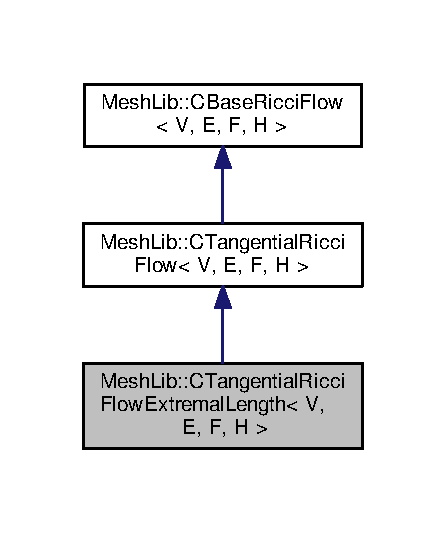
\includegraphics[width=214pt]{class_mesh_lib_1_1_c_tangential_ricci_flow_extremal_length__inherit__graph}
\end{center}
\end{figure}


Collaboration diagram for Mesh\+Lib\+:\+:C\+Tangential\+Ricci\+Flow\+Extremal\+Length$<$ V, E, F, H $>$\+:
\nopagebreak
\begin{figure}[H]
\begin{center}
\leavevmode
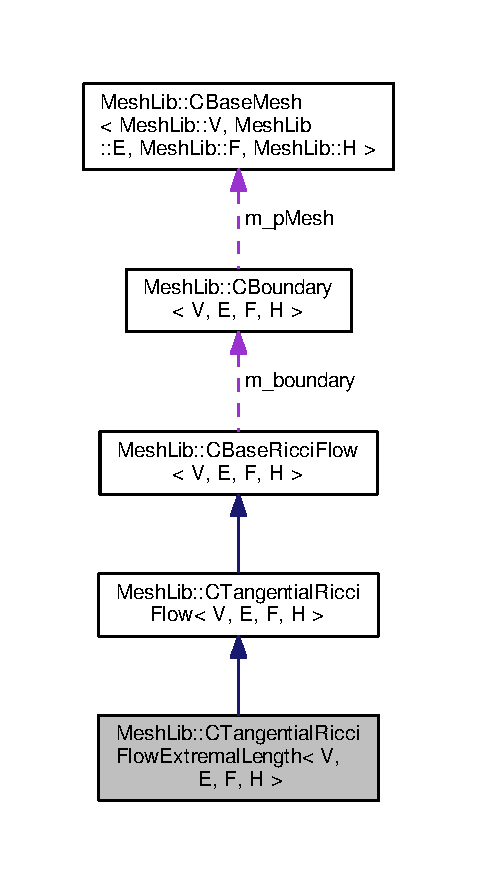
\includegraphics[width=229pt]{class_mesh_lib_1_1_c_tangential_ricci_flow_extremal_length__coll__graph}
\end{center}
\end{figure}
\subsection*{Public Member Functions}
\begin{DoxyCompactItemize}
\item 
\hyperlink{class_mesh_lib_1_1_c_tangential_ricci_flow_extremal_length_adf9a193473c13c08bb9d6644e4d3c729}{C\+Tangential\+Ricci\+Flow\+Extremal\+Length} (C\+Ricci\+Flow\+Mesh$<$ V, E, F, H $>$ $\ast$p\+Mesh)
\begin{DoxyCompactList}\small\item\em \hyperlink{class_mesh_lib_1_1_c_tangential_ricci_flow_extremal_length}{C\+Tangential\+Ricci\+Flow\+Extremal\+Length} constructor. \end{DoxyCompactList}\end{DoxyCompactItemize}
\subsection*{Protected Member Functions}
\begin{DoxyCompactItemize}
\item 
void \hyperlink{class_mesh_lib_1_1_c_tangential_ricci_flow_extremal_length_a2a1ba73cdc13bd1778ecbf89d632f691}{\+\_\+set\+\_\+target\+\_\+curvature} ()
\item 
void \hyperlink{class_mesh_lib_1_1_c_tangential_ricci_flow_extremal_length_adb8f2cf2ea4253ed325e6f35fddac975}{\+\_\+calculate\+\_\+topo\+\_\+valence} ()
\end{DoxyCompactItemize}
\subsection*{Additional Inherited Members}


\subsection{Detailed Description}
\subsubsection*{template$<$class V, class E, class F, class H$>$\\*
class Mesh\+Lib\+::\+C\+Tangential\+Ricci\+Flow\+Extremal\+Length$<$ V, E, F, H $>$}

C\+Inversive\+Distance\+Ricci\+Flow\+Extremal\+Length class. 

Algorithm for Euclidean Inversive Distance Ricci flow for Extremal Length 

Definition at line 26 of file Tangential\+Ricci\+Extremal\+Length.\+h.



\subsection{Constructor \& Destructor Documentation}
\index{Mesh\+Lib\+::\+C\+Tangential\+Ricci\+Flow\+Extremal\+Length@{Mesh\+Lib\+::\+C\+Tangential\+Ricci\+Flow\+Extremal\+Length}!C\+Tangential\+Ricci\+Flow\+Extremal\+Length@{C\+Tangential\+Ricci\+Flow\+Extremal\+Length}}
\index{C\+Tangential\+Ricci\+Flow\+Extremal\+Length@{C\+Tangential\+Ricci\+Flow\+Extremal\+Length}!Mesh\+Lib\+::\+C\+Tangential\+Ricci\+Flow\+Extremal\+Length@{Mesh\+Lib\+::\+C\+Tangential\+Ricci\+Flow\+Extremal\+Length}}
\subsubsection[{\texorpdfstring{C\+Tangential\+Ricci\+Flow\+Extremal\+Length(\+C\+Ricci\+Flow\+Mesh$<$ V, E, F, H $>$ $\ast$p\+Mesh)}{CTangentialRicciFlowExtremalLength(CRicciFlowMesh< V, E, F, H > *pMesh)}}]{\setlength{\rightskip}{0pt plus 5cm}template$<$class V , class E , class F , class H $>$ {\bf Mesh\+Lib\+::\+C\+Tangential\+Ricci\+Flow\+Extremal\+Length}$<$ V, E, F, H $>$\+::{\bf C\+Tangential\+Ricci\+Flow\+Extremal\+Length} (
\begin{DoxyParamCaption}
\item[{C\+Ricci\+Flow\+Mesh$<$ V, E, F, H $>$ $\ast$}]{p\+Mesh}
\end{DoxyParamCaption}
)}\hypertarget{class_mesh_lib_1_1_c_tangential_ricci_flow_extremal_length_adf9a193473c13c08bb9d6644e4d3c729}{}\label{class_mesh_lib_1_1_c_tangential_ricci_flow_extremal_length_adf9a193473c13c08bb9d6644e4d3c729}


\hyperlink{class_mesh_lib_1_1_c_tangential_ricci_flow_extremal_length}{C\+Tangential\+Ricci\+Flow\+Extremal\+Length} constructor. 

call base class constructor 

Definition at line 49 of file Tangential\+Ricci\+Extremal\+Length.\+h.



\subsection{Member Function Documentation}
\index{Mesh\+Lib\+::\+C\+Tangential\+Ricci\+Flow\+Extremal\+Length@{Mesh\+Lib\+::\+C\+Tangential\+Ricci\+Flow\+Extremal\+Length}!\+\_\+calculate\+\_\+topo\+\_\+valence@{\+\_\+calculate\+\_\+topo\+\_\+valence}}
\index{\+\_\+calculate\+\_\+topo\+\_\+valence@{\+\_\+calculate\+\_\+topo\+\_\+valence}!Mesh\+Lib\+::\+C\+Tangential\+Ricci\+Flow\+Extremal\+Length@{Mesh\+Lib\+::\+C\+Tangential\+Ricci\+Flow\+Extremal\+Length}}
\subsubsection[{\texorpdfstring{\+\_\+calculate\+\_\+topo\+\_\+valence()}{_calculate_topo_valence()}}]{\setlength{\rightskip}{0pt plus 5cm}template$<$class V , class E , class F , class H $>$ void {\bf Mesh\+Lib\+::\+C\+Tangential\+Ricci\+Flow\+Extremal\+Length}$<$ V, E, F, H $>$\+::\+\_\+calculate\+\_\+topo\+\_\+valence (
\begin{DoxyParamCaption}
{}
\end{DoxyParamCaption}
)\hspace{0.3cm}{\ttfamily [protected]}}\hypertarget{class_mesh_lib_1_1_c_tangential_ricci_flow_extremal_length_adb8f2cf2ea4253ed325e6f35fddac975}{}\label{class_mesh_lib_1_1_c_tangential_ricci_flow_extremal_length_adb8f2cf2ea4253ed325e6f35fddac975}
compute the vertex topological valence 

Definition at line 56 of file Tangential\+Ricci\+Extremal\+Length.\+h.

\index{Mesh\+Lib\+::\+C\+Tangential\+Ricci\+Flow\+Extremal\+Length@{Mesh\+Lib\+::\+C\+Tangential\+Ricci\+Flow\+Extremal\+Length}!\+\_\+set\+\_\+target\+\_\+curvature@{\+\_\+set\+\_\+target\+\_\+curvature}}
\index{\+\_\+set\+\_\+target\+\_\+curvature@{\+\_\+set\+\_\+target\+\_\+curvature}!Mesh\+Lib\+::\+C\+Tangential\+Ricci\+Flow\+Extremal\+Length@{Mesh\+Lib\+::\+C\+Tangential\+Ricci\+Flow\+Extremal\+Length}}
\subsubsection[{\texorpdfstring{\+\_\+set\+\_\+target\+\_\+curvature()}{_set_target_curvature()}}]{\setlength{\rightskip}{0pt plus 5cm}template$<$class V , class E , class F , class H $>$ void {\bf Mesh\+Lib\+::\+C\+Tangential\+Ricci\+Flow\+Extremal\+Length}$<$ V, E, F, H $>$\+::\+\_\+set\+\_\+target\+\_\+curvature (
\begin{DoxyParamCaption}
{}
\end{DoxyParamCaption}
)\hspace{0.3cm}{\ttfamily [protected]}, {\ttfamily [virtual]}}\hypertarget{class_mesh_lib_1_1_c_tangential_ricci_flow_extremal_length_a2a1ba73cdc13bd1778ecbf89d632f691}{}\label{class_mesh_lib_1_1_c_tangential_ricci_flow_extremal_length_a2a1ba73cdc13bd1778ecbf89d632f691}
Set the target curvature on each vertex 

Reimplemented from \hyperlink{class_mesh_lib_1_1_c_tangential_ricci_flow_ab7cbb76f7ca0de62311bc9c0cfc281e5}{Mesh\+Lib\+::\+C\+Tangential\+Ricci\+Flow$<$ V, E, F, H $>$}.



Definition at line 75 of file Tangential\+Ricci\+Extremal\+Length.\+h.



The documentation for this class was generated from the following file\+:\begin{DoxyCompactItemize}
\item 
Mesh\+Lib/algorithm/\+Riemannian/\+Ricci\+Flow/\hyperlink{_tangential_ricci_extremal_length_8h}{Tangential\+Ricci\+Extremal\+Length.\+h}\end{DoxyCompactItemize}

\hypertarget{class_mesh_lib_1_1_c_token}{}\section{Mesh\+Lib\+:\+:C\+Token Class Reference}
\label{class_mesh_lib_1_1_c_token}\index{Mesh\+Lib\+::\+C\+Token@{Mesh\+Lib\+::\+C\+Token}}


\hyperlink{class_mesh_lib_1_1_c_token}{C\+Token} class, key=(value), e.\+g. uv=(x y)  




{\ttfamily \#include $<$parser.\+h$>$}

\subsection*{Public Attributes}
\begin{DoxyCompactItemize}
\item 
std\+::string \hyperlink{class_mesh_lib_1_1_c_token_a239388f9ad2ccb0985e069754606655e}{m\+\_\+key}
\item 
std\+::string \hyperlink{class_mesh_lib_1_1_c_token_a93193611239a7d9f5eba7d002dcd93e9}{m\+\_\+value}
\end{DoxyCompactItemize}


\subsection{Detailed Description}
\hyperlink{class_mesh_lib_1_1_c_token}{C\+Token} class, key=(value), e.\+g. uv=(x y) 

Definition at line 24 of file parser.\+h.



\subsection{Member Data Documentation}
\index{Mesh\+Lib\+::\+C\+Token@{Mesh\+Lib\+::\+C\+Token}!m\+\_\+key@{m\+\_\+key}}
\index{m\+\_\+key@{m\+\_\+key}!Mesh\+Lib\+::\+C\+Token@{Mesh\+Lib\+::\+C\+Token}}
\subsubsection[{\texorpdfstring{m\+\_\+key}{m_key}}]{\setlength{\rightskip}{0pt plus 5cm}std\+::string Mesh\+Lib\+::\+C\+Token\+::m\+\_\+key}\hypertarget{class_mesh_lib_1_1_c_token_a239388f9ad2ccb0985e069754606655e}{}\label{class_mesh_lib_1_1_c_token_a239388f9ad2ccb0985e069754606655e}
key of the token 

Definition at line 28 of file parser.\+h.

\index{Mesh\+Lib\+::\+C\+Token@{Mesh\+Lib\+::\+C\+Token}!m\+\_\+value@{m\+\_\+value}}
\index{m\+\_\+value@{m\+\_\+value}!Mesh\+Lib\+::\+C\+Token@{Mesh\+Lib\+::\+C\+Token}}
\subsubsection[{\texorpdfstring{m\+\_\+value}{m_value}}]{\setlength{\rightskip}{0pt plus 5cm}std\+::string Mesh\+Lib\+::\+C\+Token\+::m\+\_\+value}\hypertarget{class_mesh_lib_1_1_c_token_a93193611239a7d9f5eba7d002dcd93e9}{}\label{class_mesh_lib_1_1_c_token_a93193611239a7d9f5eba7d002dcd93e9}
value of the token 

Definition at line 30 of file parser.\+h.



The documentation for this class was generated from the following file\+:\begin{DoxyCompactItemize}
\item 
Mesh\+Lib/core/\+Parser/\hyperlink{parser_8h}{parser.\+h}\end{DoxyCompactItemize}

\hypertarget{class_mesh_lib_1_1_c_vertex}{}\section{Mesh\+Lib\+:\+:C\+Vertex Class Reference}
\label{class_mesh_lib_1_1_c_vertex}\index{Mesh\+Lib\+::\+C\+Vertex@{Mesh\+Lib\+::\+C\+Vertex}}


\hyperlink{class_mesh_lib_1_1_c_vertex}{C\+Vertex} class, which is the base class of all kinds of vertex classes.  




{\ttfamily \#include $<$Vertex.\+h$>$}



Inheritance diagram for Mesh\+Lib\+:\+:C\+Vertex\+:
\nopagebreak
\begin{figure}[H]
\begin{center}
\leavevmode
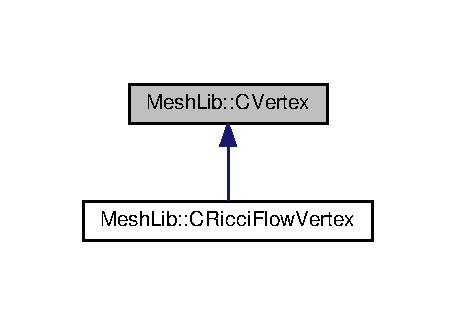
\includegraphics[width=219pt]{class_mesh_lib_1_1_c_vertex__inherit__graph}
\end{center}
\end{figure}


Collaboration diagram for Mesh\+Lib\+:\+:C\+Vertex\+:
\nopagebreak
\begin{figure}[H]
\begin{center}
\leavevmode
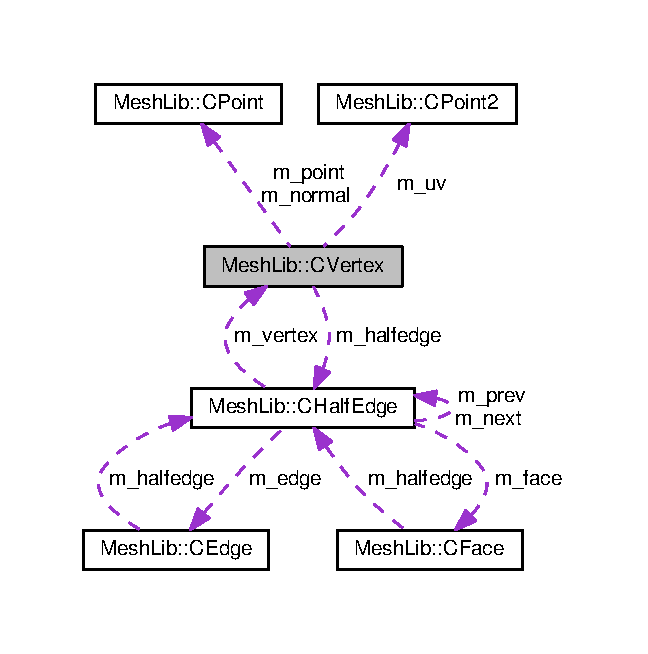
\includegraphics[width=311pt]{class_mesh_lib_1_1_c_vertex__coll__graph}
\end{center}
\end{figure}
\subsection*{Public Member Functions}
\begin{DoxyCompactItemize}
\item 
\hyperlink{class_mesh_lib_1_1_c_vertex_ac97920fc9fe1786a2199b02e0bdcea27}{C\+Vertex} ()
\item 
\hyperlink{class_mesh_lib_1_1_c_vertex_a7e93bbcd7e264d336f1e935b466118d5}{$\sim$\+C\+Vertex} ()
\item 
\hyperlink{class_mesh_lib_1_1_c_point}{C\+Point} \& \hyperlink{class_mesh_lib_1_1_c_vertex_aee899036f88e50121d455b37e4345fad}{point} ()
\item 
\hyperlink{class_mesh_lib_1_1_c_point}{C\+Point} \& \hyperlink{class_mesh_lib_1_1_c_vertex_ad969307c4a9e91e8a7a19d2f16bbdd03}{normal} ()
\item 
\hyperlink{class_mesh_lib_1_1_c_point2}{C\+Point2} \& \hyperlink{class_mesh_lib_1_1_c_vertex_aebb4e0369c2d1c21f2f46287a0c9e4d5}{uv} ()
\item 
\hyperlink{class_mesh_lib_1_1_c_half_edge}{C\+Half\+Edge} $\ast$ \hyperlink{class_mesh_lib_1_1_c_vertex_a2de79af92df8f39c851e811c2ee20b09}{most\+\_\+ccw\+\_\+out\+\_\+halfedge} ()
\item 
\hyperlink{class_mesh_lib_1_1_c_half_edge}{C\+Half\+Edge} $\ast$ \hyperlink{class_mesh_lib_1_1_c_vertex_af5fd1d56b98c3e6b1e6c29b2a40067f7}{most\+\_\+clw\+\_\+out\+\_\+halfedge} ()
\item 
\hyperlink{class_mesh_lib_1_1_c_half_edge}{C\+Half\+Edge} $\ast$ \hyperlink{class_mesh_lib_1_1_c_vertex_ae25573c3fc9a3a1ff08f95ed637879d1}{most\+\_\+ccw\+\_\+in\+\_\+halfedge} ()
\begin{DoxyCompactList}\small\item\em The most counter clockwise incoming halfedge of the vertex. \end{DoxyCompactList}\item 
\hyperlink{class_mesh_lib_1_1_c_half_edge}{C\+Half\+Edge} $\ast$ \hyperlink{class_mesh_lib_1_1_c_vertex_a88f960be654aa5d907bca82846baf83f}{most\+\_\+clw\+\_\+in\+\_\+halfedge} ()
\item 
\hyperlink{class_mesh_lib_1_1_c_half_edge}{C\+Half\+Edge} $\ast$\& \hyperlink{class_mesh_lib_1_1_c_vertex_a9329743f6b46a232759cfc41263d89cf}{halfedge} ()
\item 
std\+::string \& \hyperlink{class_mesh_lib_1_1_c_vertex_a6f5a20dd30404c47f118364c60fd1867}{string} ()
\item 
int \& \hyperlink{class_mesh_lib_1_1_c_vertex_a90179a85f86617e62fa57d0157e38c77}{id} ()
\item 
bool \& \hyperlink{class_mesh_lib_1_1_c_vertex_a1bfd813474ce6f0347c442412c3bb650}{boundary} ()
\item 
void \hyperlink{class_mesh_lib_1_1_c_vertex_a16b808933a970ac84776d404d21ecaee}{\+\_\+to\+\_\+string} ()
\item 
void \hyperlink{class_mesh_lib_1_1_c_vertex_a89670e5392950fcbeb467fa5f7a8c88a}{\+\_\+from\+\_\+string} ()
\item 
std\+::list$<$ \hyperlink{class_mesh_lib_1_1_c_edge}{C\+Edge} $\ast$ $>$ \& \hyperlink{class_mesh_lib_1_1_c_vertex_a03ec8f7820f2f3f6cd0a97f1958197c8}{edges} ()
\end{DoxyCompactItemize}
\subsection*{Protected Attributes}
\begin{DoxyCompactItemize}
\item 
int \hyperlink{class_mesh_lib_1_1_c_vertex_a686d33c96343be3d7b9c46b628061bd9}{m\+\_\+id}
\item 
\hyperlink{class_mesh_lib_1_1_c_point}{C\+Point} \hyperlink{class_mesh_lib_1_1_c_vertex_a0611ed63a1451d3077bcb2dbaf5f1e89}{m\+\_\+point}
\item 
\hyperlink{class_mesh_lib_1_1_c_point}{C\+Point} \hyperlink{class_mesh_lib_1_1_c_vertex_aa313fb31475b4951f50e50f141cec0fc}{m\+\_\+normal}
\item 
\hyperlink{class_mesh_lib_1_1_c_point2}{C\+Point2} \hyperlink{class_mesh_lib_1_1_c_vertex_a8509cd466e9db87b76b2571783d111a2}{m\+\_\+uv}
\item 
\hyperlink{class_mesh_lib_1_1_c_half_edge}{C\+Half\+Edge} $\ast$ \hyperlink{class_mesh_lib_1_1_c_vertex_a322a95750dc442c4559ef180d35a6074}{m\+\_\+halfedge}
\item 
bool \hyperlink{class_mesh_lib_1_1_c_vertex_a82467ff3e1f8bf16972a1b63326441c3}{m\+\_\+boundary}
\item 
std\+::string \hyperlink{class_mesh_lib_1_1_c_vertex_a0ad694c0749eb9b71c0faaafde732d3e}{m\+\_\+string}
\item 
std\+::list$<$ \hyperlink{class_mesh_lib_1_1_c_edge}{C\+Edge} $\ast$ $>$ \hyperlink{class_mesh_lib_1_1_c_vertex_ac6914ef1d52a245340b8bd07e671c87d}{m\+\_\+edges}
\end{DoxyCompactItemize}


\subsection{Detailed Description}
\hyperlink{class_mesh_lib_1_1_c_vertex}{C\+Vertex} class, which is the base class of all kinds of vertex classes. 

Definition at line 27 of file Vertex.\+h.



\subsection{Constructor \& Destructor Documentation}
\index{Mesh\+Lib\+::\+C\+Vertex@{Mesh\+Lib\+::\+C\+Vertex}!C\+Vertex@{C\+Vertex}}
\index{C\+Vertex@{C\+Vertex}!Mesh\+Lib\+::\+C\+Vertex@{Mesh\+Lib\+::\+C\+Vertex}}
\subsubsection[{\texorpdfstring{C\+Vertex()}{CVertex()}}]{\setlength{\rightskip}{0pt plus 5cm}Mesh\+Lib\+::\+C\+Vertex\+::\+C\+Vertex (
\begin{DoxyParamCaption}
{}
\end{DoxyParamCaption}
)\hspace{0.3cm}{\ttfamily [inline]}}\hypertarget{class_mesh_lib_1_1_c_vertex_ac97920fc9fe1786a2199b02e0bdcea27}{}\label{class_mesh_lib_1_1_c_vertex_ac97920fc9fe1786a2199b02e0bdcea27}
\hyperlink{class_mesh_lib_1_1_c_vertex}{C\+Vertex} constructor 

Definition at line 33 of file Vertex.\+h.

\index{Mesh\+Lib\+::\+C\+Vertex@{Mesh\+Lib\+::\+C\+Vertex}!````~C\+Vertex@{$\sim$\+C\+Vertex}}
\index{````~C\+Vertex@{$\sim$\+C\+Vertex}!Mesh\+Lib\+::\+C\+Vertex@{Mesh\+Lib\+::\+C\+Vertex}}
\subsubsection[{\texorpdfstring{$\sim$\+C\+Vertex()}{~CVertex()}}]{\setlength{\rightskip}{0pt plus 5cm}Mesh\+Lib\+::\+C\+Vertex\+::$\sim$\+C\+Vertex (
\begin{DoxyParamCaption}
{}
\end{DoxyParamCaption}
)\hspace{0.3cm}{\ttfamily [inline]}}\hypertarget{class_mesh_lib_1_1_c_vertex_a7e93bbcd7e264d336f1e935b466118d5}{}\label{class_mesh_lib_1_1_c_vertex_a7e93bbcd7e264d336f1e935b466118d5}
\hyperlink{class_mesh_lib_1_1_c_vertex}{C\+Vertex} destructor 

Definition at line 37 of file Vertex.\+h.



\subsection{Member Function Documentation}
\index{Mesh\+Lib\+::\+C\+Vertex@{Mesh\+Lib\+::\+C\+Vertex}!\+\_\+from\+\_\+string@{\+\_\+from\+\_\+string}}
\index{\+\_\+from\+\_\+string@{\+\_\+from\+\_\+string}!Mesh\+Lib\+::\+C\+Vertex@{Mesh\+Lib\+::\+C\+Vertex}}
\subsubsection[{\texorpdfstring{\+\_\+from\+\_\+string()}{_from_string()}}]{\setlength{\rightskip}{0pt plus 5cm}void Mesh\+Lib\+::\+C\+Vertex\+::\+\_\+from\+\_\+string (
\begin{DoxyParamCaption}
{}
\end{DoxyParamCaption}
)\hspace{0.3cm}{\ttfamily [inline]}}\hypertarget{class_mesh_lib_1_1_c_vertex_a89670e5392950fcbeb467fa5f7a8c88a}{}\label{class_mesh_lib_1_1_c_vertex_a89670e5392950fcbeb467fa5f7a8c88a}
Read traits from the string. 

Definition at line 79 of file Vertex.\+h.

\index{Mesh\+Lib\+::\+C\+Vertex@{Mesh\+Lib\+::\+C\+Vertex}!\+\_\+to\+\_\+string@{\+\_\+to\+\_\+string}}
\index{\+\_\+to\+\_\+string@{\+\_\+to\+\_\+string}!Mesh\+Lib\+::\+C\+Vertex@{Mesh\+Lib\+::\+C\+Vertex}}
\subsubsection[{\texorpdfstring{\+\_\+to\+\_\+string()}{_to_string()}}]{\setlength{\rightskip}{0pt plus 5cm}void Mesh\+Lib\+::\+C\+Vertex\+::\+\_\+to\+\_\+string (
\begin{DoxyParamCaption}
{}
\end{DoxyParamCaption}
)\hspace{0.3cm}{\ttfamily [inline]}}\hypertarget{class_mesh_lib_1_1_c_vertex_a16b808933a970ac84776d404d21ecaee}{}\label{class_mesh_lib_1_1_c_vertex_a16b808933a970ac84776d404d21ecaee}
Convert vertex traits to string. 

Definition at line 76 of file Vertex.\+h.

\index{Mesh\+Lib\+::\+C\+Vertex@{Mesh\+Lib\+::\+C\+Vertex}!boundary@{boundary}}
\index{boundary@{boundary}!Mesh\+Lib\+::\+C\+Vertex@{Mesh\+Lib\+::\+C\+Vertex}}
\subsubsection[{\texorpdfstring{boundary()}{boundary()}}]{\setlength{\rightskip}{0pt plus 5cm}bool\& Mesh\+Lib\+::\+C\+Vertex\+::boundary (
\begin{DoxyParamCaption}
{}
\end{DoxyParamCaption}
)\hspace{0.3cm}{\ttfamily [inline]}}\hypertarget{class_mesh_lib_1_1_c_vertex_a1bfd813474ce6f0347c442412c3bb650}{}\label{class_mesh_lib_1_1_c_vertex_a1bfd813474ce6f0347c442412c3bb650}
Whether the vertex is on the boundary. 

Definition at line 73 of file Vertex.\+h.

\index{Mesh\+Lib\+::\+C\+Vertex@{Mesh\+Lib\+::\+C\+Vertex}!edges@{edges}}
\index{edges@{edges}!Mesh\+Lib\+::\+C\+Vertex@{Mesh\+Lib\+::\+C\+Vertex}}
\subsubsection[{\texorpdfstring{edges()}{edges()}}]{\setlength{\rightskip}{0pt plus 5cm}std\+::list$<${\bf C\+Edge}$\ast$$>$\& Mesh\+Lib\+::\+C\+Vertex\+::edges (
\begin{DoxyParamCaption}
{}
\end{DoxyParamCaption}
)\hspace{0.3cm}{\ttfamily [inline]}}\hypertarget{class_mesh_lib_1_1_c_vertex_a03ec8f7820f2f3f6cd0a97f1958197c8}{}\label{class_mesh_lib_1_1_c_vertex_a03ec8f7820f2f3f6cd0a97f1958197c8}
Adjacent edges, temporarily used for loading the mesh 

Definition at line 83 of file Vertex.\+h.

\index{Mesh\+Lib\+::\+C\+Vertex@{Mesh\+Lib\+::\+C\+Vertex}!halfedge@{halfedge}}
\index{halfedge@{halfedge}!Mesh\+Lib\+::\+C\+Vertex@{Mesh\+Lib\+::\+C\+Vertex}}
\subsubsection[{\texorpdfstring{halfedge()}{halfedge()}}]{\setlength{\rightskip}{0pt plus 5cm}{\bf C\+Half\+Edge}$\ast$ \& Mesh\+Lib\+::\+C\+Vertex\+::halfedge (
\begin{DoxyParamCaption}
{}
\end{DoxyParamCaption}
)\hspace{0.3cm}{\ttfamily [inline]}}\hypertarget{class_mesh_lib_1_1_c_vertex_a9329743f6b46a232759cfc41263d89cf}{}\label{class_mesh_lib_1_1_c_vertex_a9329743f6b46a232759cfc41263d89cf}
One incoming halfedge of the vertex . 

Definition at line 64 of file Vertex.\+h.

\index{Mesh\+Lib\+::\+C\+Vertex@{Mesh\+Lib\+::\+C\+Vertex}!id@{id}}
\index{id@{id}!Mesh\+Lib\+::\+C\+Vertex@{Mesh\+Lib\+::\+C\+Vertex}}
\subsubsection[{\texorpdfstring{id()}{id()}}]{\setlength{\rightskip}{0pt plus 5cm}int\& Mesh\+Lib\+::\+C\+Vertex\+::id (
\begin{DoxyParamCaption}
{}
\end{DoxyParamCaption}
)\hspace{0.3cm}{\ttfamily [inline]}}\hypertarget{class_mesh_lib_1_1_c_vertex_a90179a85f86617e62fa57d0157e38c77}{}\label{class_mesh_lib_1_1_c_vertex_a90179a85f86617e62fa57d0157e38c77}
Vertex id. 

Definition at line 70 of file Vertex.\+h.

\index{Mesh\+Lib\+::\+C\+Vertex@{Mesh\+Lib\+::\+C\+Vertex}!most\+\_\+ccw\+\_\+in\+\_\+halfedge@{most\+\_\+ccw\+\_\+in\+\_\+halfedge}}
\index{most\+\_\+ccw\+\_\+in\+\_\+halfedge@{most\+\_\+ccw\+\_\+in\+\_\+halfedge}!Mesh\+Lib\+::\+C\+Vertex@{Mesh\+Lib\+::\+C\+Vertex}}
\subsubsection[{\texorpdfstring{most\+\_\+ccw\+\_\+in\+\_\+halfedge()}{most_ccw_in_halfedge()}}]{\setlength{\rightskip}{0pt plus 5cm}{\bf C\+Half\+Edge} $\ast$ Mesh\+Lib\+::\+C\+Vertex\+::most\+\_\+ccw\+\_\+in\+\_\+halfedge (
\begin{DoxyParamCaption}
{}
\end{DoxyParamCaption}
)\hspace{0.3cm}{\ttfamily [inline]}}\hypertarget{class_mesh_lib_1_1_c_vertex_ae25573c3fc9a3a1ff08f95ed637879d1}{}\label{class_mesh_lib_1_1_c_vertex_ae25573c3fc9a3a1ff08f95ed637879d1}


The most counter clockwise incoming halfedge of the vertex. 

The most counter clockwise incoming halfedge of the vertex.

\begin{DoxyReturn}{Returns}
the most C\+CW in halfedge 
\end{DoxyReturn}


Definition at line 118 of file Vertex.\+h.

\index{Mesh\+Lib\+::\+C\+Vertex@{Mesh\+Lib\+::\+C\+Vertex}!most\+\_\+ccw\+\_\+out\+\_\+halfedge@{most\+\_\+ccw\+\_\+out\+\_\+halfedge}}
\index{most\+\_\+ccw\+\_\+out\+\_\+halfedge@{most\+\_\+ccw\+\_\+out\+\_\+halfedge}!Mesh\+Lib\+::\+C\+Vertex@{Mesh\+Lib\+::\+C\+Vertex}}
\subsubsection[{\texorpdfstring{most\+\_\+ccw\+\_\+out\+\_\+halfedge()}{most_ccw_out_halfedge()}}]{\setlength{\rightskip}{0pt plus 5cm}{\bf C\+Half\+Edge} $\ast$ Mesh\+Lib\+::\+C\+Vertex\+::most\+\_\+ccw\+\_\+out\+\_\+halfedge (
\begin{DoxyParamCaption}
{}
\end{DoxyParamCaption}
)\hspace{0.3cm}{\ttfamily [inline]}}\hypertarget{class_mesh_lib_1_1_c_vertex_a2de79af92df8f39c851e811c2ee20b09}{}\label{class_mesh_lib_1_1_c_vertex_a2de79af92df8f39c851e811c2ee20b09}
The most counter clockwise outgoing halfedge of the vertex . 

Definition at line 161 of file Vertex.\+h.

\index{Mesh\+Lib\+::\+C\+Vertex@{Mesh\+Lib\+::\+C\+Vertex}!most\+\_\+clw\+\_\+in\+\_\+halfedge@{most\+\_\+clw\+\_\+in\+\_\+halfedge}}
\index{most\+\_\+clw\+\_\+in\+\_\+halfedge@{most\+\_\+clw\+\_\+in\+\_\+halfedge}!Mesh\+Lib\+::\+C\+Vertex@{Mesh\+Lib\+::\+C\+Vertex}}
\subsubsection[{\texorpdfstring{most\+\_\+clw\+\_\+in\+\_\+halfedge()}{most_clw_in_halfedge()}}]{\setlength{\rightskip}{0pt plus 5cm}{\bf C\+Half\+Edge} $\ast$ Mesh\+Lib\+::\+C\+Vertex\+::most\+\_\+clw\+\_\+in\+\_\+halfedge (
\begin{DoxyParamCaption}
{}
\end{DoxyParamCaption}
)\hspace{0.3cm}{\ttfamily [inline]}}\hypertarget{class_mesh_lib_1_1_c_vertex_a88f960be654aa5d907bca82846baf83f}{}\label{class_mesh_lib_1_1_c_vertex_a88f960be654aa5d907bca82846baf83f}
The most clockwise incoming halfedge of the vertex. 

Definition at line 140 of file Vertex.\+h.

\index{Mesh\+Lib\+::\+C\+Vertex@{Mesh\+Lib\+::\+C\+Vertex}!most\+\_\+clw\+\_\+out\+\_\+halfedge@{most\+\_\+clw\+\_\+out\+\_\+halfedge}}
\index{most\+\_\+clw\+\_\+out\+\_\+halfedge@{most\+\_\+clw\+\_\+out\+\_\+halfedge}!Mesh\+Lib\+::\+C\+Vertex@{Mesh\+Lib\+::\+C\+Vertex}}
\subsubsection[{\texorpdfstring{most\+\_\+clw\+\_\+out\+\_\+halfedge()}{most_clw_out_halfedge()}}]{\setlength{\rightskip}{0pt plus 5cm}{\bf C\+Half\+Edge} $\ast$ Mesh\+Lib\+::\+C\+Vertex\+::most\+\_\+clw\+\_\+out\+\_\+halfedge (
\begin{DoxyParamCaption}
{}
\end{DoxyParamCaption}
)\hspace{0.3cm}{\ttfamily [inline]}}\hypertarget{class_mesh_lib_1_1_c_vertex_af5fd1d56b98c3e6b1e6c29b2a40067f7}{}\label{class_mesh_lib_1_1_c_vertex_af5fd1d56b98c3e6b1e6c29b2a40067f7}
The most clockwise outgoing halfedge of the vertex . 

Definition at line 185 of file Vertex.\+h.

\index{Mesh\+Lib\+::\+C\+Vertex@{Mesh\+Lib\+::\+C\+Vertex}!normal@{normal}}
\index{normal@{normal}!Mesh\+Lib\+::\+C\+Vertex@{Mesh\+Lib\+::\+C\+Vertex}}
\subsubsection[{\texorpdfstring{normal()}{normal()}}]{\setlength{\rightskip}{0pt plus 5cm}{\bf C\+Point}\& Mesh\+Lib\+::\+C\+Vertex\+::normal (
\begin{DoxyParamCaption}
{}
\end{DoxyParamCaption}
)\hspace{0.3cm}{\ttfamily [inline]}}\hypertarget{class_mesh_lib_1_1_c_vertex_ad969307c4a9e91e8a7a19d2f16bbdd03}{}\label{class_mesh_lib_1_1_c_vertex_ad969307c4a9e91e8a7a19d2f16bbdd03}
The normal of the vertex 

Definition at line 44 of file Vertex.\+h.

\index{Mesh\+Lib\+::\+C\+Vertex@{Mesh\+Lib\+::\+C\+Vertex}!point@{point}}
\index{point@{point}!Mesh\+Lib\+::\+C\+Vertex@{Mesh\+Lib\+::\+C\+Vertex}}
\subsubsection[{\texorpdfstring{point()}{point()}}]{\setlength{\rightskip}{0pt plus 5cm}{\bf C\+Point}\& Mesh\+Lib\+::\+C\+Vertex\+::point (
\begin{DoxyParamCaption}
{}
\end{DoxyParamCaption}
)\hspace{0.3cm}{\ttfamily [inline]}}\hypertarget{class_mesh_lib_1_1_c_vertex_aee899036f88e50121d455b37e4345fad}{}\label{class_mesh_lib_1_1_c_vertex_aee899036f88e50121d455b37e4345fad}
The point of the vertex 

Definition at line 41 of file Vertex.\+h.

\index{Mesh\+Lib\+::\+C\+Vertex@{Mesh\+Lib\+::\+C\+Vertex}!string@{string}}
\index{string@{string}!Mesh\+Lib\+::\+C\+Vertex@{Mesh\+Lib\+::\+C\+Vertex}}
\subsubsection[{\texorpdfstring{string()}{string()}}]{\setlength{\rightskip}{0pt plus 5cm}std\+::string\& Mesh\+Lib\+::\+C\+Vertex\+::string (
\begin{DoxyParamCaption}
{}
\end{DoxyParamCaption}
)\hspace{0.3cm}{\ttfamily [inline]}}\hypertarget{class_mesh_lib_1_1_c_vertex_a6f5a20dd30404c47f118364c60fd1867}{}\label{class_mesh_lib_1_1_c_vertex_a6f5a20dd30404c47f118364c60fd1867}
the string of the vertex. 

Definition at line 67 of file Vertex.\+h.

\index{Mesh\+Lib\+::\+C\+Vertex@{Mesh\+Lib\+::\+C\+Vertex}!uv@{uv}}
\index{uv@{uv}!Mesh\+Lib\+::\+C\+Vertex@{Mesh\+Lib\+::\+C\+Vertex}}
\subsubsection[{\texorpdfstring{uv()}{uv()}}]{\setlength{\rightskip}{0pt plus 5cm}{\bf C\+Point2}\& Mesh\+Lib\+::\+C\+Vertex\+::uv (
\begin{DoxyParamCaption}
{}
\end{DoxyParamCaption}
)\hspace{0.3cm}{\ttfamily [inline]}}\hypertarget{class_mesh_lib_1_1_c_vertex_aebb4e0369c2d1c21f2f46287a0c9e4d5}{}\label{class_mesh_lib_1_1_c_vertex_aebb4e0369c2d1c21f2f46287a0c9e4d5}
The texutre coordinates of the vertex 

Definition at line 47 of file Vertex.\+h.



\subsection{Member Data Documentation}
\index{Mesh\+Lib\+::\+C\+Vertex@{Mesh\+Lib\+::\+C\+Vertex}!m\+\_\+boundary@{m\+\_\+boundary}}
\index{m\+\_\+boundary@{m\+\_\+boundary}!Mesh\+Lib\+::\+C\+Vertex@{Mesh\+Lib\+::\+C\+Vertex}}
\subsubsection[{\texorpdfstring{m\+\_\+boundary}{m_boundary}}]{\setlength{\rightskip}{0pt plus 5cm}bool Mesh\+Lib\+::\+C\+Vertex\+::m\+\_\+boundary\hspace{0.3cm}{\ttfamily [protected]}}\hypertarget{class_mesh_lib_1_1_c_vertex_a82467ff3e1f8bf16972a1b63326441c3}{}\label{class_mesh_lib_1_1_c_vertex_a82467ff3e1f8bf16972a1b63326441c3}
Indicating if the vertex is on the boundary. 

Definition at line 103 of file Vertex.\+h.

\index{Mesh\+Lib\+::\+C\+Vertex@{Mesh\+Lib\+::\+C\+Vertex}!m\+\_\+edges@{m\+\_\+edges}}
\index{m\+\_\+edges@{m\+\_\+edges}!Mesh\+Lib\+::\+C\+Vertex@{Mesh\+Lib\+::\+C\+Vertex}}
\subsubsection[{\texorpdfstring{m\+\_\+edges}{m_edges}}]{\setlength{\rightskip}{0pt plus 5cm}std\+::list$<${\bf C\+Edge}$\ast$$>$ Mesh\+Lib\+::\+C\+Vertex\+::m\+\_\+edges\hspace{0.3cm}{\ttfamily [protected]}}\hypertarget{class_mesh_lib_1_1_c_vertex_ac6914ef1d52a245340b8bd07e671c87d}{}\label{class_mesh_lib_1_1_c_vertex_ac6914ef1d52a245340b8bd07e671c87d}
List of adjacent edges, such that current vertex is the end vertex of the edge with smaller id 

Definition at line 110 of file Vertex.\+h.

\index{Mesh\+Lib\+::\+C\+Vertex@{Mesh\+Lib\+::\+C\+Vertex}!m\+\_\+halfedge@{m\+\_\+halfedge}}
\index{m\+\_\+halfedge@{m\+\_\+halfedge}!Mesh\+Lib\+::\+C\+Vertex@{Mesh\+Lib\+::\+C\+Vertex}}
\subsubsection[{\texorpdfstring{m\+\_\+halfedge}{m_halfedge}}]{\setlength{\rightskip}{0pt plus 5cm}{\bf C\+Half\+Edge}$\ast$ Mesh\+Lib\+::\+C\+Vertex\+::m\+\_\+halfedge\hspace{0.3cm}{\ttfamily [protected]}}\hypertarget{class_mesh_lib_1_1_c_vertex_a322a95750dc442c4559ef180d35a6074}{}\label{class_mesh_lib_1_1_c_vertex_a322a95750dc442c4559ef180d35a6074}
The most C\+CW incoming halfedge of the vertex. 

Definition at line 100 of file Vertex.\+h.

\index{Mesh\+Lib\+::\+C\+Vertex@{Mesh\+Lib\+::\+C\+Vertex}!m\+\_\+id@{m\+\_\+id}}
\index{m\+\_\+id@{m\+\_\+id}!Mesh\+Lib\+::\+C\+Vertex@{Mesh\+Lib\+::\+C\+Vertex}}
\subsubsection[{\texorpdfstring{m\+\_\+id}{m_id}}]{\setlength{\rightskip}{0pt plus 5cm}int Mesh\+Lib\+::\+C\+Vertex\+::m\+\_\+id\hspace{0.3cm}{\ttfamily [protected]}}\hypertarget{class_mesh_lib_1_1_c_vertex_a686d33c96343be3d7b9c46b628061bd9}{}\label{class_mesh_lib_1_1_c_vertex_a686d33c96343be3d7b9c46b628061bd9}
Vertex ID. 

Definition at line 83 of file Vertex.\+h.

\index{Mesh\+Lib\+::\+C\+Vertex@{Mesh\+Lib\+::\+C\+Vertex}!m\+\_\+normal@{m\+\_\+normal}}
\index{m\+\_\+normal@{m\+\_\+normal}!Mesh\+Lib\+::\+C\+Vertex@{Mesh\+Lib\+::\+C\+Vertex}}
\subsubsection[{\texorpdfstring{m\+\_\+normal}{m_normal}}]{\setlength{\rightskip}{0pt plus 5cm}{\bf C\+Point} Mesh\+Lib\+::\+C\+Vertex\+::m\+\_\+normal\hspace{0.3cm}{\ttfamily [protected]}}\hypertarget{class_mesh_lib_1_1_c_vertex_aa313fb31475b4951f50e50f141cec0fc}{}\label{class_mesh_lib_1_1_c_vertex_aa313fb31475b4951f50e50f141cec0fc}
Normal at the vertex. 

Definition at line 94 of file Vertex.\+h.

\index{Mesh\+Lib\+::\+C\+Vertex@{Mesh\+Lib\+::\+C\+Vertex}!m\+\_\+point@{m\+\_\+point}}
\index{m\+\_\+point@{m\+\_\+point}!Mesh\+Lib\+::\+C\+Vertex@{Mesh\+Lib\+::\+C\+Vertex}}
\subsubsection[{\texorpdfstring{m\+\_\+point}{m_point}}]{\setlength{\rightskip}{0pt plus 5cm}{\bf C\+Point} Mesh\+Lib\+::\+C\+Vertex\+::m\+\_\+point\hspace{0.3cm}{\ttfamily [protected]}}\hypertarget{class_mesh_lib_1_1_c_vertex_a0611ed63a1451d3077bcb2dbaf5f1e89}{}\label{class_mesh_lib_1_1_c_vertex_a0611ed63a1451d3077bcb2dbaf5f1e89}
Vertex position point. 

Definition at line 91 of file Vertex.\+h.

\index{Mesh\+Lib\+::\+C\+Vertex@{Mesh\+Lib\+::\+C\+Vertex}!m\+\_\+string@{m\+\_\+string}}
\index{m\+\_\+string@{m\+\_\+string}!Mesh\+Lib\+::\+C\+Vertex@{Mesh\+Lib\+::\+C\+Vertex}}
\subsubsection[{\texorpdfstring{m\+\_\+string}{m_string}}]{\setlength{\rightskip}{0pt plus 5cm}std\+::string Mesh\+Lib\+::\+C\+Vertex\+::m\+\_\+string\hspace{0.3cm}{\ttfamily [protected]}}\hypertarget{class_mesh_lib_1_1_c_vertex_a0ad694c0749eb9b71c0faaafde732d3e}{}\label{class_mesh_lib_1_1_c_vertex_a0ad694c0749eb9b71c0faaafde732d3e}
The string of the vertex, which stores the traits information. 

Definition at line 106 of file Vertex.\+h.

\index{Mesh\+Lib\+::\+C\+Vertex@{Mesh\+Lib\+::\+C\+Vertex}!m\+\_\+uv@{m\+\_\+uv}}
\index{m\+\_\+uv@{m\+\_\+uv}!Mesh\+Lib\+::\+C\+Vertex@{Mesh\+Lib\+::\+C\+Vertex}}
\subsubsection[{\texorpdfstring{m\+\_\+uv}{m_uv}}]{\setlength{\rightskip}{0pt plus 5cm}{\bf C\+Point2} Mesh\+Lib\+::\+C\+Vertex\+::m\+\_\+uv\hspace{0.3cm}{\ttfamily [protected]}}\hypertarget{class_mesh_lib_1_1_c_vertex_a8509cd466e9db87b76b2571783d111a2}{}\label{class_mesh_lib_1_1_c_vertex_a8509cd466e9db87b76b2571783d111a2}
Texture coordinates of the vertex. 

Definition at line 97 of file Vertex.\+h.



The documentation for this class was generated from the following file\+:\begin{DoxyCompactItemize}
\item 
Mesh\+Lib/core/\+Mesh/\hyperlink{_vertex_8h}{Vertex.\+h}\end{DoxyCompactItemize}

\hypertarget{class_mesh_lib_1_1_face_edge_iterator}{}\section{Mesh\+Lib\+:\+:Face\+Edge\+Iterator$<$ C\+Vertex, C\+Edge, C\+Face, C\+Half\+Edge $>$ Class Template Reference}
\label{class_mesh_lib_1_1_face_edge_iterator}\index{Mesh\+Lib\+::\+Face\+Edge\+Iterator$<$ C\+Vertex, C\+Edge, C\+Face, C\+Half\+Edge $>$@{Mesh\+Lib\+::\+Face\+Edge\+Iterator$<$ C\+Vertex, C\+Edge, C\+Face, C\+Half\+Edge $>$}}


\hyperlink{class_mesh_lib_1_1_face_edge_iterator}{Face\+Edge\+Iterator}, transverse all the edges of a face C\+C\+Wly.  




{\ttfamily \#include $<$iterators.\+h$>$}

\subsection*{Public Member Functions}
\begin{DoxyCompactItemize}
\item 
\hyperlink{class_mesh_lib_1_1_face_edge_iterator_a73b6a961906309febf686830999e5b9b}{Face\+Edge\+Iterator} (\hyperlink{class_mesh_lib_1_1_c_face}{C\+Face} $\ast$f)
\item 
\hyperlink{class_mesh_lib_1_1_face_edge_iterator_abbc2d0f2fa3d6f160640870b0e7875bb}{$\sim$\+Face\+Edge\+Iterator} ()
\item 
void \hyperlink{class_mesh_lib_1_1_face_edge_iterator_a62c91827805723e19ded7a85edf1625b}{operator++} ()
\item 
void \hyperlink{class_mesh_lib_1_1_face_edge_iterator_ab44f25c24611bf61f35d42687c23e502}{operator++} (int)
\item 
\hyperlink{class_mesh_lib_1_1_c_edge}{C\+Edge} $\ast$ \hyperlink{class_mesh_lib_1_1_face_edge_iterator_a84357c09fa86c7382ffc1b64f47dc601}{value} ()
\item 
\hyperlink{class_mesh_lib_1_1_c_edge}{C\+Edge} $\ast$ \hyperlink{class_mesh_lib_1_1_face_edge_iterator_af592c6a6fd3154aa3492db9f4b20c9c3}{operator$\ast$} ()
\item 
bool \hyperlink{class_mesh_lib_1_1_face_edge_iterator_a84af7266112582d76a84cb979523d0a1}{end} ()
\end{DoxyCompactItemize}


\subsection{Detailed Description}
\subsubsection*{template$<$class C\+Vertex, class C\+Edge, class C\+Face, class C\+Half\+Edge$>$\\*
class Mesh\+Lib\+::\+Face\+Edge\+Iterator$<$ C\+Vertex, C\+Edge, C\+Face, C\+Half\+Edge $>$}

\hyperlink{class_mesh_lib_1_1_face_edge_iterator}{Face\+Edge\+Iterator}, transverse all the edges of a face C\+C\+Wly. 

Definition at line 631 of file iterators.\+h.



\subsection{Constructor \& Destructor Documentation}
\index{Mesh\+Lib\+::\+Face\+Edge\+Iterator@{Mesh\+Lib\+::\+Face\+Edge\+Iterator}!Face\+Edge\+Iterator@{Face\+Edge\+Iterator}}
\index{Face\+Edge\+Iterator@{Face\+Edge\+Iterator}!Mesh\+Lib\+::\+Face\+Edge\+Iterator@{Mesh\+Lib\+::\+Face\+Edge\+Iterator}}
\subsubsection[{\texorpdfstring{Face\+Edge\+Iterator(\+C\+Face $\ast$f)}{FaceEdgeIterator(CFace *f)}}]{\setlength{\rightskip}{0pt plus 5cm}template$<$class C\+Vertex , class C\+Edge , class C\+Face , class C\+Half\+Edge $>$ {\bf Mesh\+Lib\+::\+Face\+Edge\+Iterator}$<$ {\bf C\+Vertex}, {\bf C\+Edge}, {\bf C\+Face}, {\bf C\+Half\+Edge} $>$\+::{\bf Face\+Edge\+Iterator} (
\begin{DoxyParamCaption}
\item[{{\bf C\+Face} $\ast$}]{f}
\end{DoxyParamCaption}
)\hspace{0.3cm}{\ttfamily [inline]}}\hypertarget{class_mesh_lib_1_1_face_edge_iterator_a73b6a961906309febf686830999e5b9b}{}\label{class_mesh_lib_1_1_face_edge_iterator_a73b6a961906309febf686830999e5b9b}
\hyperlink{class_mesh_lib_1_1_face_edge_iterator}{Face\+Edge\+Iterator} constructor 
\begin{DoxyParams}{Parameters}
{\em f} & the current face \\
\hline
\end{DoxyParams}


Definition at line 638 of file iterators.\+h.

\index{Mesh\+Lib\+::\+Face\+Edge\+Iterator@{Mesh\+Lib\+::\+Face\+Edge\+Iterator}!````~Face\+Edge\+Iterator@{$\sim$\+Face\+Edge\+Iterator}}
\index{````~Face\+Edge\+Iterator@{$\sim$\+Face\+Edge\+Iterator}!Mesh\+Lib\+::\+Face\+Edge\+Iterator@{Mesh\+Lib\+::\+Face\+Edge\+Iterator}}
\subsubsection[{\texorpdfstring{$\sim$\+Face\+Edge\+Iterator()}{~FaceEdgeIterator()}}]{\setlength{\rightskip}{0pt plus 5cm}template$<$class C\+Vertex , class C\+Edge , class C\+Face , class C\+Half\+Edge $>$ {\bf Mesh\+Lib\+::\+Face\+Edge\+Iterator}$<$ {\bf C\+Vertex}, {\bf C\+Edge}, {\bf C\+Face}, {\bf C\+Half\+Edge} $>$\+::$\sim${\bf Face\+Edge\+Iterator} (
\begin{DoxyParamCaption}
{}
\end{DoxyParamCaption}
)\hspace{0.3cm}{\ttfamily [inline]}}\hypertarget{class_mesh_lib_1_1_face_edge_iterator_abbc2d0f2fa3d6f160640870b0e7875bb}{}\label{class_mesh_lib_1_1_face_edge_iterator_abbc2d0f2fa3d6f160640870b0e7875bb}
\hyperlink{class_mesh_lib_1_1_face_edge_iterator}{Face\+Edge\+Iterator} destructor 

Definition at line 647 of file iterators.\+h.



\subsection{Member Function Documentation}
\index{Mesh\+Lib\+::\+Face\+Edge\+Iterator@{Mesh\+Lib\+::\+Face\+Edge\+Iterator}!end@{end}}
\index{end@{end}!Mesh\+Lib\+::\+Face\+Edge\+Iterator@{Mesh\+Lib\+::\+Face\+Edge\+Iterator}}
\subsubsection[{\texorpdfstring{end()}{end()}}]{\setlength{\rightskip}{0pt plus 5cm}template$<$class C\+Vertex , class C\+Edge , class C\+Face , class C\+Half\+Edge $>$ bool {\bf Mesh\+Lib\+::\+Face\+Edge\+Iterator}$<$ {\bf C\+Vertex}, {\bf C\+Edge}, {\bf C\+Face}, {\bf C\+Half\+Edge} $>$\+::end (
\begin{DoxyParamCaption}
{}
\end{DoxyParamCaption}
)\hspace{0.3cm}{\ttfamily [inline]}}\hypertarget{class_mesh_lib_1_1_face_edge_iterator_a84af7266112582d76a84cb979523d0a1}{}\label{class_mesh_lib_1_1_face_edge_iterator_a84af7266112582d76a84cb979523d0a1}
Indicate whether all the edges have been transversed. 

Definition at line 688 of file iterators.\+h.

\index{Mesh\+Lib\+::\+Face\+Edge\+Iterator@{Mesh\+Lib\+::\+Face\+Edge\+Iterator}!operator$\ast$@{operator$\ast$}}
\index{operator$\ast$@{operator$\ast$}!Mesh\+Lib\+::\+Face\+Edge\+Iterator@{Mesh\+Lib\+::\+Face\+Edge\+Iterator}}
\subsubsection[{\texorpdfstring{operator$\ast$()}{operator*()}}]{\setlength{\rightskip}{0pt plus 5cm}template$<$class C\+Vertex , class C\+Edge , class C\+Face , class C\+Half\+Edge $>$ {\bf C\+Edge}$\ast$ {\bf Mesh\+Lib\+::\+Face\+Edge\+Iterator}$<$ {\bf C\+Vertex}, {\bf C\+Edge}, {\bf C\+Face}, {\bf C\+Half\+Edge} $>$\+::operator$\ast$ (
\begin{DoxyParamCaption}
{}
\end{DoxyParamCaption}
)\hspace{0.3cm}{\ttfamily [inline]}}\hypertarget{class_mesh_lib_1_1_face_edge_iterator_af592c6a6fd3154aa3492db9f4b20c9c3}{}\label{class_mesh_lib_1_1_face_edge_iterator_af592c6a6fd3154aa3492db9f4b20c9c3}
The edge, pointed by the current iterator 

Definition at line 684 of file iterators.\+h.

\index{Mesh\+Lib\+::\+Face\+Edge\+Iterator@{Mesh\+Lib\+::\+Face\+Edge\+Iterator}!operator++@{operator++}}
\index{operator++@{operator++}!Mesh\+Lib\+::\+Face\+Edge\+Iterator@{Mesh\+Lib\+::\+Face\+Edge\+Iterator}}
\subsubsection[{\texorpdfstring{operator++()}{operator++()}}]{\setlength{\rightskip}{0pt plus 5cm}template$<$class C\+Vertex , class C\+Edge , class C\+Face , class C\+Half\+Edge $>$ void {\bf Mesh\+Lib\+::\+Face\+Edge\+Iterator}$<$ {\bf C\+Vertex}, {\bf C\+Edge}, {\bf C\+Face}, {\bf C\+Half\+Edge} $>$\+::operator++ (
\begin{DoxyParamCaption}
{}
\end{DoxyParamCaption}
)\hspace{0.3cm}{\ttfamily [inline]}}\hypertarget{class_mesh_lib_1_1_face_edge_iterator_a62c91827805723e19ded7a85edf1625b}{}\label{class_mesh_lib_1_1_face_edge_iterator_a62c91827805723e19ded7a85edf1625b}
\hyperlink{class_mesh_lib_1_1_face_edge_iterator}{Face\+Edge\+Iterator} prefix operator ++, goes to the next edge C\+C\+Wly 

Definition at line 651 of file iterators.\+h.

\index{Mesh\+Lib\+::\+Face\+Edge\+Iterator@{Mesh\+Lib\+::\+Face\+Edge\+Iterator}!operator++@{operator++}}
\index{operator++@{operator++}!Mesh\+Lib\+::\+Face\+Edge\+Iterator@{Mesh\+Lib\+::\+Face\+Edge\+Iterator}}
\subsubsection[{\texorpdfstring{operator++(int)}{operator++(int)}}]{\setlength{\rightskip}{0pt plus 5cm}template$<$class C\+Vertex , class C\+Edge , class C\+Face , class C\+Half\+Edge $>$ void {\bf Mesh\+Lib\+::\+Face\+Edge\+Iterator}$<$ {\bf C\+Vertex}, {\bf C\+Edge}, {\bf C\+Face}, {\bf C\+Half\+Edge} $>$\+::operator++ (
\begin{DoxyParamCaption}
\item[{int}]{}
\end{DoxyParamCaption}
)\hspace{0.3cm}{\ttfamily [inline]}}\hypertarget{class_mesh_lib_1_1_face_edge_iterator_ab44f25c24611bf61f35d42687c23e502}{}\label{class_mesh_lib_1_1_face_edge_iterator_ab44f25c24611bf61f35d42687c23e502}
\hyperlink{class_mesh_lib_1_1_face_edge_iterator}{Face\+Edge\+Iterator} prefix operator ++, goes to the next edge C\+C\+Wly 

Definition at line 666 of file iterators.\+h.

\index{Mesh\+Lib\+::\+Face\+Edge\+Iterator@{Mesh\+Lib\+::\+Face\+Edge\+Iterator}!value@{value}}
\index{value@{value}!Mesh\+Lib\+::\+Face\+Edge\+Iterator@{Mesh\+Lib\+::\+Face\+Edge\+Iterator}}
\subsubsection[{\texorpdfstring{value()}{value()}}]{\setlength{\rightskip}{0pt plus 5cm}template$<$class C\+Vertex , class C\+Edge , class C\+Face , class C\+Half\+Edge $>$ {\bf C\+Edge}$\ast$ {\bf Mesh\+Lib\+::\+Face\+Edge\+Iterator}$<$ {\bf C\+Vertex}, {\bf C\+Edge}, {\bf C\+Face}, {\bf C\+Half\+Edge} $>$\+::value (
\begin{DoxyParamCaption}
{}
\end{DoxyParamCaption}
)\hspace{0.3cm}{\ttfamily [inline]}}\hypertarget{class_mesh_lib_1_1_face_edge_iterator_a84357c09fa86c7382ffc1b64f47dc601}{}\label{class_mesh_lib_1_1_face_edge_iterator_a84357c09fa86c7382ffc1b64f47dc601}
The edge, pointed by the current iterator 

Definition at line 680 of file iterators.\+h.



The documentation for this class was generated from the following file\+:\begin{DoxyCompactItemize}
\item 
Mesh\+Lib/core/\+Mesh/\hyperlink{iterators_8h}{iterators.\+h}\end{DoxyCompactItemize}

\hypertarget{class_mesh_lib_1_1_face_halfedge_iterator}{}\section{Mesh\+Lib\+:\+:Face\+Halfedge\+Iterator$<$ C\+Vertex, C\+Edge, C\+Face, C\+Half\+Edge $>$ Class Template Reference}
\label{class_mesh_lib_1_1_face_halfedge_iterator}\index{Mesh\+Lib\+::\+Face\+Halfedge\+Iterator$<$ C\+Vertex, C\+Edge, C\+Face, C\+Half\+Edge $>$@{Mesh\+Lib\+::\+Face\+Halfedge\+Iterator$<$ C\+Vertex, C\+Edge, C\+Face, C\+Half\+Edge $>$}}


\hyperlink{class_mesh_lib_1_1_face_halfedge_iterator}{Face\+Halfedge\+Iterator}, transverse all the halfedges of a face C\+C\+Wly.  




{\ttfamily \#include $<$iterators.\+h$>$}

\subsection*{Public Member Functions}
\begin{DoxyCompactItemize}
\item 
\hyperlink{class_mesh_lib_1_1_face_halfedge_iterator_ad0206cbb7214b717bbc625bab2b54f5e}{Face\+Halfedge\+Iterator} (\hyperlink{class_mesh_lib_1_1_c_face}{C\+Face} $\ast$f)
\item 
\hyperlink{class_mesh_lib_1_1_face_halfedge_iterator_ac309d80e77edba4b83cb3c365ac5713f}{$\sim$\+Face\+Halfedge\+Iterator} ()
\item 
void \hyperlink{class_mesh_lib_1_1_face_halfedge_iterator_ad9957d1e32cb93adce990fb978d0331c}{operator++} ()
\item 
void \hyperlink{class_mesh_lib_1_1_face_halfedge_iterator_aa086c815a7f0aee20dd7f619103bd130}{operator++} (int)
\item 
\hyperlink{class_mesh_lib_1_1_c_half_edge}{C\+Half\+Edge} $\ast$ \hyperlink{class_mesh_lib_1_1_face_halfedge_iterator_a11ab5569fee0954568104005ad63db80}{value} ()
\item 
\hyperlink{class_mesh_lib_1_1_c_half_edge}{C\+Half\+Edge} $\ast$ \hyperlink{class_mesh_lib_1_1_face_halfedge_iterator_a4a893aa715532f4c13cdde4e13fcff81}{operator$\ast$} ()
\item 
bool \hyperlink{class_mesh_lib_1_1_face_halfedge_iterator_af899bde10dcb1883ac26e66930fc3082}{end} ()
\end{DoxyCompactItemize}


\subsection{Detailed Description}
\subsubsection*{template$<$class C\+Vertex, class C\+Edge, class C\+Face, class C\+Half\+Edge$>$\\*
class Mesh\+Lib\+::\+Face\+Halfedge\+Iterator$<$ C\+Vertex, C\+Edge, C\+Face, C\+Half\+Edge $>$}

\hyperlink{class_mesh_lib_1_1_face_halfedge_iterator}{Face\+Halfedge\+Iterator}, transverse all the halfedges of a face C\+C\+Wly. 

Definition at line 553 of file iterators.\+h.



\subsection{Constructor \& Destructor Documentation}
\index{Mesh\+Lib\+::\+Face\+Halfedge\+Iterator@{Mesh\+Lib\+::\+Face\+Halfedge\+Iterator}!Face\+Halfedge\+Iterator@{Face\+Halfedge\+Iterator}}
\index{Face\+Halfedge\+Iterator@{Face\+Halfedge\+Iterator}!Mesh\+Lib\+::\+Face\+Halfedge\+Iterator@{Mesh\+Lib\+::\+Face\+Halfedge\+Iterator}}
\subsubsection[{\texorpdfstring{Face\+Halfedge\+Iterator(\+C\+Face $\ast$f)}{FaceHalfedgeIterator(CFace *f)}}]{\setlength{\rightskip}{0pt plus 5cm}template$<$class C\+Vertex , class C\+Edge , class C\+Face , class C\+Half\+Edge $>$ {\bf Mesh\+Lib\+::\+Face\+Halfedge\+Iterator}$<$ {\bf C\+Vertex}, {\bf C\+Edge}, {\bf C\+Face}, {\bf C\+Half\+Edge} $>$\+::{\bf Face\+Halfedge\+Iterator} (
\begin{DoxyParamCaption}
\item[{{\bf C\+Face} $\ast$}]{f}
\end{DoxyParamCaption}
)\hspace{0.3cm}{\ttfamily [inline]}}\hypertarget{class_mesh_lib_1_1_face_halfedge_iterator_ad0206cbb7214b717bbc625bab2b54f5e}{}\label{class_mesh_lib_1_1_face_halfedge_iterator_ad0206cbb7214b717bbc625bab2b54f5e}
\hyperlink{class_mesh_lib_1_1_face_halfedge_iterator}{Face\+Halfedge\+Iterator} constructor 
\begin{DoxyParams}{Parameters}
{\em f} & the current face \\
\hline
\end{DoxyParams}


Definition at line 560 of file iterators.\+h.

\index{Mesh\+Lib\+::\+Face\+Halfedge\+Iterator@{Mesh\+Lib\+::\+Face\+Halfedge\+Iterator}!````~Face\+Halfedge\+Iterator@{$\sim$\+Face\+Halfedge\+Iterator}}
\index{````~Face\+Halfedge\+Iterator@{$\sim$\+Face\+Halfedge\+Iterator}!Mesh\+Lib\+::\+Face\+Halfedge\+Iterator@{Mesh\+Lib\+::\+Face\+Halfedge\+Iterator}}
\subsubsection[{\texorpdfstring{$\sim$\+Face\+Halfedge\+Iterator()}{~FaceHalfedgeIterator()}}]{\setlength{\rightskip}{0pt plus 5cm}template$<$class C\+Vertex , class C\+Edge , class C\+Face , class C\+Half\+Edge $>$ {\bf Mesh\+Lib\+::\+Face\+Halfedge\+Iterator}$<$ {\bf C\+Vertex}, {\bf C\+Edge}, {\bf C\+Face}, {\bf C\+Half\+Edge} $>$\+::$\sim${\bf Face\+Halfedge\+Iterator} (
\begin{DoxyParamCaption}
{}
\end{DoxyParamCaption}
)\hspace{0.3cm}{\ttfamily [inline]}}\hypertarget{class_mesh_lib_1_1_face_halfedge_iterator_ac309d80e77edba4b83cb3c365ac5713f}{}\label{class_mesh_lib_1_1_face_halfedge_iterator_ac309d80e77edba4b83cb3c365ac5713f}
\hyperlink{class_mesh_lib_1_1_face_halfedge_iterator}{Face\+Halfedge\+Iterator} destructor 

Definition at line 568 of file iterators.\+h.



\subsection{Member Function Documentation}
\index{Mesh\+Lib\+::\+Face\+Halfedge\+Iterator@{Mesh\+Lib\+::\+Face\+Halfedge\+Iterator}!end@{end}}
\index{end@{end}!Mesh\+Lib\+::\+Face\+Halfedge\+Iterator@{Mesh\+Lib\+::\+Face\+Halfedge\+Iterator}}
\subsubsection[{\texorpdfstring{end()}{end()}}]{\setlength{\rightskip}{0pt plus 5cm}template$<$class C\+Vertex , class C\+Edge , class C\+Face , class C\+Half\+Edge $>$ bool {\bf Mesh\+Lib\+::\+Face\+Halfedge\+Iterator}$<$ {\bf C\+Vertex}, {\bf C\+Edge}, {\bf C\+Face}, {\bf C\+Half\+Edge} $>$\+::end (
\begin{DoxyParamCaption}
{}
\end{DoxyParamCaption}
)\hspace{0.3cm}{\ttfamily [inline]}}\hypertarget{class_mesh_lib_1_1_face_halfedge_iterator_af899bde10dcb1883ac26e66930fc3082}{}\label{class_mesh_lib_1_1_face_halfedge_iterator_af899bde10dcb1883ac26e66930fc3082}
Indicate whether all the halfedges have been accessed. 

Definition at line 611 of file iterators.\+h.

\index{Mesh\+Lib\+::\+Face\+Halfedge\+Iterator@{Mesh\+Lib\+::\+Face\+Halfedge\+Iterator}!operator$\ast$@{operator$\ast$}}
\index{operator$\ast$@{operator$\ast$}!Mesh\+Lib\+::\+Face\+Halfedge\+Iterator@{Mesh\+Lib\+::\+Face\+Halfedge\+Iterator}}
\subsubsection[{\texorpdfstring{operator$\ast$()}{operator*()}}]{\setlength{\rightskip}{0pt plus 5cm}template$<$class C\+Vertex , class C\+Edge , class C\+Face , class C\+Half\+Edge $>$ {\bf C\+Half\+Edge}$\ast$ {\bf Mesh\+Lib\+::\+Face\+Halfedge\+Iterator}$<$ {\bf C\+Vertex}, {\bf C\+Edge}, {\bf C\+Face}, {\bf C\+Half\+Edge} $>$\+::operator$\ast$ (
\begin{DoxyParamCaption}
{}
\end{DoxyParamCaption}
)\hspace{0.3cm}{\ttfamily [inline]}}\hypertarget{class_mesh_lib_1_1_face_halfedge_iterator_a4a893aa715532f4c13cdde4e13fcff81}{}\label{class_mesh_lib_1_1_face_halfedge_iterator_a4a893aa715532f4c13cdde4e13fcff81}
The halfedge, pointed by the current iterator 

Definition at line 606 of file iterators.\+h.

\index{Mesh\+Lib\+::\+Face\+Halfedge\+Iterator@{Mesh\+Lib\+::\+Face\+Halfedge\+Iterator}!operator++@{operator++}}
\index{operator++@{operator++}!Mesh\+Lib\+::\+Face\+Halfedge\+Iterator@{Mesh\+Lib\+::\+Face\+Halfedge\+Iterator}}
\subsubsection[{\texorpdfstring{operator++()}{operator++()}}]{\setlength{\rightskip}{0pt plus 5cm}template$<$class C\+Vertex , class C\+Edge , class C\+Face , class C\+Half\+Edge $>$ void {\bf Mesh\+Lib\+::\+Face\+Halfedge\+Iterator}$<$ {\bf C\+Vertex}, {\bf C\+Edge}, {\bf C\+Face}, {\bf C\+Half\+Edge} $>$\+::operator++ (
\begin{DoxyParamCaption}
{}
\end{DoxyParamCaption}
)\hspace{0.3cm}{\ttfamily [inline]}}\hypertarget{class_mesh_lib_1_1_face_halfedge_iterator_ad9957d1e32cb93adce990fb978d0331c}{}\label{class_mesh_lib_1_1_face_halfedge_iterator_ad9957d1e32cb93adce990fb978d0331c}
\hyperlink{class_mesh_lib_1_1_vertex_vertex_iterator}{Vertex\+Vertex\+Iterator} prefix operator ++, goes to the next halfedge C\+C\+Wly 

Definition at line 572 of file iterators.\+h.

\index{Mesh\+Lib\+::\+Face\+Halfedge\+Iterator@{Mesh\+Lib\+::\+Face\+Halfedge\+Iterator}!operator++@{operator++}}
\index{operator++@{operator++}!Mesh\+Lib\+::\+Face\+Halfedge\+Iterator@{Mesh\+Lib\+::\+Face\+Halfedge\+Iterator}}
\subsubsection[{\texorpdfstring{operator++(int)}{operator++(int)}}]{\setlength{\rightskip}{0pt plus 5cm}template$<$class C\+Vertex , class C\+Edge , class C\+Face , class C\+Half\+Edge $>$ void {\bf Mesh\+Lib\+::\+Face\+Halfedge\+Iterator}$<$ {\bf C\+Vertex}, {\bf C\+Edge}, {\bf C\+Face}, {\bf C\+Half\+Edge} $>$\+::operator++ (
\begin{DoxyParamCaption}
\item[{int}]{}
\end{DoxyParamCaption}
)\hspace{0.3cm}{\ttfamily [inline]}}\hypertarget{class_mesh_lib_1_1_face_halfedge_iterator_aa086c815a7f0aee20dd7f619103bd130}{}\label{class_mesh_lib_1_1_face_halfedge_iterator_aa086c815a7f0aee20dd7f619103bd130}
\hyperlink{class_mesh_lib_1_1_vertex_vertex_iterator}{Vertex\+Vertex\+Iterator} prefix operator ++, goes to the next halfedge C\+C\+Wly 

Definition at line 587 of file iterators.\+h.

\index{Mesh\+Lib\+::\+Face\+Halfedge\+Iterator@{Mesh\+Lib\+::\+Face\+Halfedge\+Iterator}!value@{value}}
\index{value@{value}!Mesh\+Lib\+::\+Face\+Halfedge\+Iterator@{Mesh\+Lib\+::\+Face\+Halfedge\+Iterator}}
\subsubsection[{\texorpdfstring{value()}{value()}}]{\setlength{\rightskip}{0pt plus 5cm}template$<$class C\+Vertex , class C\+Edge , class C\+Face , class C\+Half\+Edge $>$ {\bf C\+Half\+Edge}$\ast$ {\bf Mesh\+Lib\+::\+Face\+Halfedge\+Iterator}$<$ {\bf C\+Vertex}, {\bf C\+Edge}, {\bf C\+Face}, {\bf C\+Half\+Edge} $>$\+::value (
\begin{DoxyParamCaption}
{}
\end{DoxyParamCaption}
)\hspace{0.3cm}{\ttfamily [inline]}}\hypertarget{class_mesh_lib_1_1_face_halfedge_iterator_a11ab5569fee0954568104005ad63db80}{}\label{class_mesh_lib_1_1_face_halfedge_iterator_a11ab5569fee0954568104005ad63db80}
The halfedge, pointed by the current iterator 

Definition at line 602 of file iterators.\+h.



The documentation for this class was generated from the following file\+:\begin{DoxyCompactItemize}
\item 
Mesh\+Lib/core/\+Mesh/\hyperlink{iterators_8h}{iterators.\+h}\end{DoxyCompactItemize}

\hypertarget{class_mesh_lib_1_1_face_vertex_iterator}{}\section{Mesh\+Lib\+:\+:Face\+Vertex\+Iterator$<$ C\+Vertex, C\+Edge, C\+Face, C\+Half\+Edge $>$ Class Template Reference}
\label{class_mesh_lib_1_1_face_vertex_iterator}\index{Mesh\+Lib\+::\+Face\+Vertex\+Iterator$<$ C\+Vertex, C\+Edge, C\+Face, C\+Half\+Edge $>$@{Mesh\+Lib\+::\+Face\+Vertex\+Iterator$<$ C\+Vertex, C\+Edge, C\+Face, C\+Half\+Edge $>$}}


\hyperlink{class_mesh_lib_1_1_face_vertex_iterator}{Face\+Vertex\+Iterator}, transverse all the vertices of a face C\+C\+Wly.  




{\ttfamily \#include $<$iterators.\+h$>$}

\subsection*{Public Member Functions}
\begin{DoxyCompactItemize}
\item 
\hyperlink{class_mesh_lib_1_1_face_vertex_iterator_a5bb987960d8c4c1341e498bd271c2a9c}{Face\+Vertex\+Iterator} (\hyperlink{class_mesh_lib_1_1_c_face}{C\+Face} $\ast$f)
\item 
\hyperlink{class_mesh_lib_1_1_face_vertex_iterator_af7f5cb6d47792007453e5b70444b552e}{$\sim$\+Face\+Vertex\+Iterator} ()
\item 
void \hyperlink{class_mesh_lib_1_1_face_vertex_iterator_a48fcbdd253bd64204cd9b287570755da}{operator++} ()
\item 
void \hyperlink{class_mesh_lib_1_1_face_vertex_iterator_a80a8dc853d1c31223437d4ae67cd3b75}{operator++} (int)
\item 
\hyperlink{class_mesh_lib_1_1_c_vertex}{C\+Vertex} $\ast$ \hyperlink{class_mesh_lib_1_1_face_vertex_iterator_a703cf14713514017d9e0e227f9286b1a}{value} ()
\item 
\hyperlink{class_mesh_lib_1_1_c_vertex}{C\+Vertex} $\ast$ \hyperlink{class_mesh_lib_1_1_face_vertex_iterator_a992525a89a87402946b5eac77659cd62}{operator$\ast$} ()
\item 
bool \hyperlink{class_mesh_lib_1_1_face_vertex_iterator_abc127d0fbd0347551998a93b13b73560}{end} ()
\end{DoxyCompactItemize}


\subsection{Detailed Description}
\subsubsection*{template$<$class C\+Vertex, class C\+Edge, class C\+Face, class C\+Half\+Edge$>$\\*
class Mesh\+Lib\+::\+Face\+Vertex\+Iterator$<$ C\+Vertex, C\+Edge, C\+Face, C\+Half\+Edge $>$}

\hyperlink{class_mesh_lib_1_1_face_vertex_iterator}{Face\+Vertex\+Iterator}, transverse all the vertices of a face C\+C\+Wly. 

Definition at line 704 of file iterators.\+h.



\subsection{Constructor \& Destructor Documentation}
\index{Mesh\+Lib\+::\+Face\+Vertex\+Iterator@{Mesh\+Lib\+::\+Face\+Vertex\+Iterator}!Face\+Vertex\+Iterator@{Face\+Vertex\+Iterator}}
\index{Face\+Vertex\+Iterator@{Face\+Vertex\+Iterator}!Mesh\+Lib\+::\+Face\+Vertex\+Iterator@{Mesh\+Lib\+::\+Face\+Vertex\+Iterator}}
\subsubsection[{\texorpdfstring{Face\+Vertex\+Iterator(\+C\+Face $\ast$f)}{FaceVertexIterator(CFace *f)}}]{\setlength{\rightskip}{0pt plus 5cm}template$<$class C\+Vertex , class C\+Edge , class C\+Face , class C\+Half\+Edge $>$ {\bf Mesh\+Lib\+::\+Face\+Vertex\+Iterator}$<$ {\bf C\+Vertex}, {\bf C\+Edge}, {\bf C\+Face}, {\bf C\+Half\+Edge} $>$\+::{\bf Face\+Vertex\+Iterator} (
\begin{DoxyParamCaption}
\item[{{\bf C\+Face} $\ast$}]{f}
\end{DoxyParamCaption}
)\hspace{0.3cm}{\ttfamily [inline]}}\hypertarget{class_mesh_lib_1_1_face_vertex_iterator_a5bb987960d8c4c1341e498bd271c2a9c}{}\label{class_mesh_lib_1_1_face_vertex_iterator_a5bb987960d8c4c1341e498bd271c2a9c}
\hyperlink{class_mesh_lib_1_1_face_vertex_iterator}{Face\+Vertex\+Iterator} constructor 
\begin{DoxyParams}{Parameters}
{\em f} & the current face \\
\hline
\end{DoxyParams}


Definition at line 711 of file iterators.\+h.

\index{Mesh\+Lib\+::\+Face\+Vertex\+Iterator@{Mesh\+Lib\+::\+Face\+Vertex\+Iterator}!````~Face\+Vertex\+Iterator@{$\sim$\+Face\+Vertex\+Iterator}}
\index{````~Face\+Vertex\+Iterator@{$\sim$\+Face\+Vertex\+Iterator}!Mesh\+Lib\+::\+Face\+Vertex\+Iterator@{Mesh\+Lib\+::\+Face\+Vertex\+Iterator}}
\subsubsection[{\texorpdfstring{$\sim$\+Face\+Vertex\+Iterator()}{~FaceVertexIterator()}}]{\setlength{\rightskip}{0pt plus 5cm}template$<$class C\+Vertex , class C\+Edge , class C\+Face , class C\+Half\+Edge $>$ {\bf Mesh\+Lib\+::\+Face\+Vertex\+Iterator}$<$ {\bf C\+Vertex}, {\bf C\+Edge}, {\bf C\+Face}, {\bf C\+Half\+Edge} $>$\+::$\sim${\bf Face\+Vertex\+Iterator} (
\begin{DoxyParamCaption}
{}
\end{DoxyParamCaption}
)\hspace{0.3cm}{\ttfamily [inline]}}\hypertarget{class_mesh_lib_1_1_face_vertex_iterator_af7f5cb6d47792007453e5b70444b552e}{}\label{class_mesh_lib_1_1_face_vertex_iterator_af7f5cb6d47792007453e5b70444b552e}
\hyperlink{class_mesh_lib_1_1_face_vertex_iterator}{Face\+Vertex\+Iterator} destructor 

Definition at line 720 of file iterators.\+h.



\subsection{Member Function Documentation}
\index{Mesh\+Lib\+::\+Face\+Vertex\+Iterator@{Mesh\+Lib\+::\+Face\+Vertex\+Iterator}!end@{end}}
\index{end@{end}!Mesh\+Lib\+::\+Face\+Vertex\+Iterator@{Mesh\+Lib\+::\+Face\+Vertex\+Iterator}}
\subsubsection[{\texorpdfstring{end()}{end()}}]{\setlength{\rightskip}{0pt plus 5cm}template$<$class C\+Vertex , class C\+Edge , class C\+Face , class C\+Half\+Edge $>$ bool {\bf Mesh\+Lib\+::\+Face\+Vertex\+Iterator}$<$ {\bf C\+Vertex}, {\bf C\+Edge}, {\bf C\+Face}, {\bf C\+Half\+Edge} $>$\+::end (
\begin{DoxyParamCaption}
{}
\end{DoxyParamCaption}
)\hspace{0.3cm}{\ttfamily [inline]}}\hypertarget{class_mesh_lib_1_1_face_vertex_iterator_abc127d0fbd0347551998a93b13b73560}{}\label{class_mesh_lib_1_1_face_vertex_iterator_abc127d0fbd0347551998a93b13b73560}
Indicate whether all the vertices have been accessed. 

Definition at line 761 of file iterators.\+h.

\index{Mesh\+Lib\+::\+Face\+Vertex\+Iterator@{Mesh\+Lib\+::\+Face\+Vertex\+Iterator}!operator$\ast$@{operator$\ast$}}
\index{operator$\ast$@{operator$\ast$}!Mesh\+Lib\+::\+Face\+Vertex\+Iterator@{Mesh\+Lib\+::\+Face\+Vertex\+Iterator}}
\subsubsection[{\texorpdfstring{operator$\ast$()}{operator*()}}]{\setlength{\rightskip}{0pt plus 5cm}template$<$class C\+Vertex , class C\+Edge , class C\+Face , class C\+Half\+Edge $>$ {\bf C\+Vertex}$\ast$ {\bf Mesh\+Lib\+::\+Face\+Vertex\+Iterator}$<$ {\bf C\+Vertex}, {\bf C\+Edge}, {\bf C\+Face}, {\bf C\+Half\+Edge} $>$\+::operator$\ast$ (
\begin{DoxyParamCaption}
{}
\end{DoxyParamCaption}
)\hspace{0.3cm}{\ttfamily [inline]}}\hypertarget{class_mesh_lib_1_1_face_vertex_iterator_a992525a89a87402946b5eac77659cd62}{}\label{class_mesh_lib_1_1_face_vertex_iterator_a992525a89a87402946b5eac77659cd62}
The vertex, pointed by the current iterator 

Definition at line 757 of file iterators.\+h.

\index{Mesh\+Lib\+::\+Face\+Vertex\+Iterator@{Mesh\+Lib\+::\+Face\+Vertex\+Iterator}!operator++@{operator++}}
\index{operator++@{operator++}!Mesh\+Lib\+::\+Face\+Vertex\+Iterator@{Mesh\+Lib\+::\+Face\+Vertex\+Iterator}}
\subsubsection[{\texorpdfstring{operator++()}{operator++()}}]{\setlength{\rightskip}{0pt plus 5cm}template$<$class C\+Vertex , class C\+Edge , class C\+Face , class C\+Half\+Edge $>$ void {\bf Mesh\+Lib\+::\+Face\+Vertex\+Iterator}$<$ {\bf C\+Vertex}, {\bf C\+Edge}, {\bf C\+Face}, {\bf C\+Half\+Edge} $>$\+::operator++ (
\begin{DoxyParamCaption}
{}
\end{DoxyParamCaption}
)\hspace{0.3cm}{\ttfamily [inline]}}\hypertarget{class_mesh_lib_1_1_face_vertex_iterator_a48fcbdd253bd64204cd9b287570755da}{}\label{class_mesh_lib_1_1_face_vertex_iterator_a48fcbdd253bd64204cd9b287570755da}
\hyperlink{class_mesh_lib_1_1_face_vertex_iterator}{Face\+Vertex\+Iterator} prefix operator ++, goes to the next vertex C\+C\+Wly 

Definition at line 724 of file iterators.\+h.

\index{Mesh\+Lib\+::\+Face\+Vertex\+Iterator@{Mesh\+Lib\+::\+Face\+Vertex\+Iterator}!operator++@{operator++}}
\index{operator++@{operator++}!Mesh\+Lib\+::\+Face\+Vertex\+Iterator@{Mesh\+Lib\+::\+Face\+Vertex\+Iterator}}
\subsubsection[{\texorpdfstring{operator++(int)}{operator++(int)}}]{\setlength{\rightskip}{0pt plus 5cm}template$<$class C\+Vertex , class C\+Edge , class C\+Face , class C\+Half\+Edge $>$ void {\bf Mesh\+Lib\+::\+Face\+Vertex\+Iterator}$<$ {\bf C\+Vertex}, {\bf C\+Edge}, {\bf C\+Face}, {\bf C\+Half\+Edge} $>$\+::operator++ (
\begin{DoxyParamCaption}
\item[{int}]{}
\end{DoxyParamCaption}
)\hspace{0.3cm}{\ttfamily [inline]}}\hypertarget{class_mesh_lib_1_1_face_vertex_iterator_a80a8dc853d1c31223437d4ae67cd3b75}{}\label{class_mesh_lib_1_1_face_vertex_iterator_a80a8dc853d1c31223437d4ae67cd3b75}
\hyperlink{class_mesh_lib_1_1_face_vertex_iterator}{Face\+Vertex\+Iterator} prefix operator ++, goes to the next vertex C\+C\+Wly 

Definition at line 739 of file iterators.\+h.

\index{Mesh\+Lib\+::\+Face\+Vertex\+Iterator@{Mesh\+Lib\+::\+Face\+Vertex\+Iterator}!value@{value}}
\index{value@{value}!Mesh\+Lib\+::\+Face\+Vertex\+Iterator@{Mesh\+Lib\+::\+Face\+Vertex\+Iterator}}
\subsubsection[{\texorpdfstring{value()}{value()}}]{\setlength{\rightskip}{0pt plus 5cm}template$<$class C\+Vertex , class C\+Edge , class C\+Face , class C\+Half\+Edge $>$ {\bf C\+Vertex}$\ast$ {\bf Mesh\+Lib\+::\+Face\+Vertex\+Iterator}$<$ {\bf C\+Vertex}, {\bf C\+Edge}, {\bf C\+Face}, {\bf C\+Half\+Edge} $>$\+::value (
\begin{DoxyParamCaption}
{}
\end{DoxyParamCaption}
)\hspace{0.3cm}{\ttfamily [inline]}}\hypertarget{class_mesh_lib_1_1_face_vertex_iterator_a703cf14713514017d9e0e227f9286b1a}{}\label{class_mesh_lib_1_1_face_vertex_iterator_a703cf14713514017d9e0e227f9286b1a}
The vertex, pointed by the current iterator 

Definition at line 753 of file iterators.\+h.



The documentation for this class was generated from the following file\+:\begin{DoxyCompactItemize}
\item 
Mesh\+Lib/core/\+Mesh/\hyperlink{iterators_8h}{iterators.\+h}\end{DoxyCompactItemize}

\hypertarget{class_mesh_lib_1_1_mesh_edge_iterator}{}\section{Mesh\+Lib\+:\+:Mesh\+Edge\+Iterator$<$ C\+Vertex, C\+Edge, C\+Face, C\+Half\+Edge $>$ Class Template Reference}
\label{class_mesh_lib_1_1_mesh_edge_iterator}\index{Mesh\+Lib\+::\+Mesh\+Edge\+Iterator$<$ C\+Vertex, C\+Edge, C\+Face, C\+Half\+Edge $>$@{Mesh\+Lib\+::\+Mesh\+Edge\+Iterator$<$ C\+Vertex, C\+Edge, C\+Face, C\+Half\+Edge $>$}}


\hyperlink{class_mesh_lib_1_1_mesh_edge_iterator}{Mesh\+Edge\+Iterator}, transverse all the edges in the mesh.  




{\ttfamily \#include $<$iterators.\+h$>$}

\subsection*{Public Member Functions}
\begin{DoxyCompactItemize}
\item 
\hyperlink{class_mesh_lib_1_1_mesh_edge_iterator_aca662c1484b2bcc1769475a13969795d}{Mesh\+Edge\+Iterator} (\hyperlink{class_mesh_lib_1_1_c_base_mesh}{C\+Base\+Mesh}$<$ \hyperlink{class_mesh_lib_1_1_c_vertex}{C\+Vertex}, \hyperlink{class_mesh_lib_1_1_c_edge}{C\+Edge}, \hyperlink{class_mesh_lib_1_1_c_face}{C\+Face}, \hyperlink{class_mesh_lib_1_1_c_half_edge}{C\+Half\+Edge} $>$ $\ast$p\+Mesh)
\item 
\hyperlink{class_mesh_lib_1_1_c_edge}{C\+Edge} $\ast$ \hyperlink{class_mesh_lib_1_1_mesh_edge_iterator_adac99d2306e206a5a0d2069fad354d1f}{value} ()
\item 
\hyperlink{class_mesh_lib_1_1_c_edge}{C\+Edge} $\ast$ \hyperlink{class_mesh_lib_1_1_mesh_edge_iterator_ab63ff9aa00814e9e428c6e1e0ed6e33b}{operator$\ast$} ()
\item 
void \hyperlink{class_mesh_lib_1_1_mesh_edge_iterator_a9d16c478e6b770d114e03eed10b2d31e}{operator++} ()
\item 
void \hyperlink{class_mesh_lib_1_1_mesh_edge_iterator_aabd4c9904c21993512fbb1d3c52f7381}{operator++} (int)
\item 
bool \hyperlink{class_mesh_lib_1_1_mesh_edge_iterator_a0ad4b9b11b5d043b944818631f612039}{end} ()
\end{DoxyCompactItemize}


\subsection{Detailed Description}
\subsubsection*{template$<$class C\+Vertex, class C\+Edge, class C\+Face, class C\+Half\+Edge$>$\\*
class Mesh\+Lib\+::\+Mesh\+Edge\+Iterator$<$ C\+Vertex, C\+Edge, C\+Face, C\+Half\+Edge $>$}

\hyperlink{class_mesh_lib_1_1_mesh_edge_iterator}{Mesh\+Edge\+Iterator}, transverse all the edges in the mesh. 

Definition at line 880 of file iterators.\+h.



\subsection{Constructor \& Destructor Documentation}
\index{Mesh\+Lib\+::\+Mesh\+Edge\+Iterator@{Mesh\+Lib\+::\+Mesh\+Edge\+Iterator}!Mesh\+Edge\+Iterator@{Mesh\+Edge\+Iterator}}
\index{Mesh\+Edge\+Iterator@{Mesh\+Edge\+Iterator}!Mesh\+Lib\+::\+Mesh\+Edge\+Iterator@{Mesh\+Lib\+::\+Mesh\+Edge\+Iterator}}
\subsubsection[{\texorpdfstring{Mesh\+Edge\+Iterator(\+C\+Base\+Mesh$<$ C\+Vertex, C\+Edge, C\+Face, C\+Half\+Edge $>$ $\ast$p\+Mesh)}{MeshEdgeIterator(CBaseMesh< CVertex, CEdge, CFace, CHalfEdge > *pMesh)}}]{\setlength{\rightskip}{0pt plus 5cm}template$<$class C\+Vertex , class C\+Edge , class C\+Face , class C\+Half\+Edge $>$ {\bf Mesh\+Lib\+::\+Mesh\+Edge\+Iterator}$<$ {\bf C\+Vertex}, {\bf C\+Edge}, {\bf C\+Face}, {\bf C\+Half\+Edge} $>$\+::{\bf Mesh\+Edge\+Iterator} (
\begin{DoxyParamCaption}
\item[{{\bf C\+Base\+Mesh}$<$ {\bf C\+Vertex}, {\bf C\+Edge}, {\bf C\+Face}, {\bf C\+Half\+Edge} $>$ $\ast$}]{p\+Mesh}
\end{DoxyParamCaption}
)\hspace{0.3cm}{\ttfamily [inline]}}\hypertarget{class_mesh_lib_1_1_mesh_edge_iterator_aca662c1484b2bcc1769475a13969795d}{}\label{class_mesh_lib_1_1_mesh_edge_iterator_aca662c1484b2bcc1769475a13969795d}
\hyperlink{class_mesh_lib_1_1_mesh_edge_iterator}{Mesh\+Edge\+Iterator} constructor, 
\begin{DoxyParams}{Parameters}
{\em p\+Mesh} & the current mesh \\
\hline
\end{DoxyParams}


Definition at line 887 of file iterators.\+h.



\subsection{Member Function Documentation}
\index{Mesh\+Lib\+::\+Mesh\+Edge\+Iterator@{Mesh\+Lib\+::\+Mesh\+Edge\+Iterator}!end@{end}}
\index{end@{end}!Mesh\+Lib\+::\+Mesh\+Edge\+Iterator@{Mesh\+Lib\+::\+Mesh\+Edge\+Iterator}}
\subsubsection[{\texorpdfstring{end()}{end()}}]{\setlength{\rightskip}{0pt plus 5cm}template$<$class C\+Vertex , class C\+Edge , class C\+Face , class C\+Half\+Edge $>$ bool {\bf Mesh\+Lib\+::\+Mesh\+Edge\+Iterator}$<$ {\bf C\+Vertex}, {\bf C\+Edge}, {\bf C\+Face}, {\bf C\+Half\+Edge} $>$\+::end (
\begin{DoxyParamCaption}
{}
\end{DoxyParamCaption}
)\hspace{0.3cm}{\ttfamily [inline]}}\hypertarget{class_mesh_lib_1_1_mesh_edge_iterator_a0ad4b9b11b5d043b944818631f612039}{}\label{class_mesh_lib_1_1_mesh_edge_iterator_a0ad4b9b11b5d043b944818631f612039}
Indicate whether all the edges have been accessed. 

Definition at line 911 of file iterators.\+h.

\index{Mesh\+Lib\+::\+Mesh\+Edge\+Iterator@{Mesh\+Lib\+::\+Mesh\+Edge\+Iterator}!operator$\ast$@{operator$\ast$}}
\index{operator$\ast$@{operator$\ast$}!Mesh\+Lib\+::\+Mesh\+Edge\+Iterator@{Mesh\+Lib\+::\+Mesh\+Edge\+Iterator}}
\subsubsection[{\texorpdfstring{operator$\ast$()}{operator*()}}]{\setlength{\rightskip}{0pt plus 5cm}template$<$class C\+Vertex , class C\+Edge , class C\+Face , class C\+Half\+Edge $>$ {\bf C\+Edge}$\ast$ {\bf Mesh\+Lib\+::\+Mesh\+Edge\+Iterator}$<$ {\bf C\+Vertex}, {\bf C\+Edge}, {\bf C\+Face}, {\bf C\+Half\+Edge} $>$\+::operator$\ast$ (
\begin{DoxyParamCaption}
{}
\end{DoxyParamCaption}
)\hspace{0.3cm}{\ttfamily [inline]}}\hypertarget{class_mesh_lib_1_1_mesh_edge_iterator_ab63ff9aa00814e9e428c6e1e0ed6e33b}{}\label{class_mesh_lib_1_1_mesh_edge_iterator_ab63ff9aa00814e9e428c6e1e0ed6e33b}
The edge, pointed by the current iterator 

Definition at line 899 of file iterators.\+h.

\index{Mesh\+Lib\+::\+Mesh\+Edge\+Iterator@{Mesh\+Lib\+::\+Mesh\+Edge\+Iterator}!operator++@{operator++}}
\index{operator++@{operator++}!Mesh\+Lib\+::\+Mesh\+Edge\+Iterator@{Mesh\+Lib\+::\+Mesh\+Edge\+Iterator}}
\subsubsection[{\texorpdfstring{operator++()}{operator++()}}]{\setlength{\rightskip}{0pt plus 5cm}template$<$class C\+Vertex , class C\+Edge , class C\+Face , class C\+Half\+Edge $>$ void {\bf Mesh\+Lib\+::\+Mesh\+Edge\+Iterator}$<$ {\bf C\+Vertex}, {\bf C\+Edge}, {\bf C\+Face}, {\bf C\+Half\+Edge} $>$\+::operator++ (
\begin{DoxyParamCaption}
{}
\end{DoxyParamCaption}
)\hspace{0.3cm}{\ttfamily [inline]}}\hypertarget{class_mesh_lib_1_1_mesh_edge_iterator_a9d16c478e6b770d114e03eed10b2d31e}{}\label{class_mesh_lib_1_1_mesh_edge_iterator_a9d16c478e6b770d114e03eed10b2d31e}
\hyperlink{class_mesh_lib_1_1_mesh_edge_iterator}{Mesh\+Edge\+Iterator} prefix operator ++, goes to the next edge 

Definition at line 903 of file iterators.\+h.

\index{Mesh\+Lib\+::\+Mesh\+Edge\+Iterator@{Mesh\+Lib\+::\+Mesh\+Edge\+Iterator}!operator++@{operator++}}
\index{operator++@{operator++}!Mesh\+Lib\+::\+Mesh\+Edge\+Iterator@{Mesh\+Lib\+::\+Mesh\+Edge\+Iterator}}
\subsubsection[{\texorpdfstring{operator++(int)}{operator++(int)}}]{\setlength{\rightskip}{0pt plus 5cm}template$<$class C\+Vertex , class C\+Edge , class C\+Face , class C\+Half\+Edge $>$ void {\bf Mesh\+Lib\+::\+Mesh\+Edge\+Iterator}$<$ {\bf C\+Vertex}, {\bf C\+Edge}, {\bf C\+Face}, {\bf C\+Half\+Edge} $>$\+::operator++ (
\begin{DoxyParamCaption}
\item[{int}]{}
\end{DoxyParamCaption}
)\hspace{0.3cm}{\ttfamily [inline]}}\hypertarget{class_mesh_lib_1_1_mesh_edge_iterator_aabd4c9904c21993512fbb1d3c52f7381}{}\label{class_mesh_lib_1_1_mesh_edge_iterator_aabd4c9904c21993512fbb1d3c52f7381}
\hyperlink{class_mesh_lib_1_1_mesh_edge_iterator}{Mesh\+Edge\+Iterator} postfix operator ++, goes to the next edge 

Definition at line 907 of file iterators.\+h.

\index{Mesh\+Lib\+::\+Mesh\+Edge\+Iterator@{Mesh\+Lib\+::\+Mesh\+Edge\+Iterator}!value@{value}}
\index{value@{value}!Mesh\+Lib\+::\+Mesh\+Edge\+Iterator@{Mesh\+Lib\+::\+Mesh\+Edge\+Iterator}}
\subsubsection[{\texorpdfstring{value()}{value()}}]{\setlength{\rightskip}{0pt plus 5cm}template$<$class C\+Vertex , class C\+Edge , class C\+Face , class C\+Half\+Edge $>$ {\bf C\+Edge}$\ast$ {\bf Mesh\+Lib\+::\+Mesh\+Edge\+Iterator}$<$ {\bf C\+Vertex}, {\bf C\+Edge}, {\bf C\+Face}, {\bf C\+Half\+Edge} $>$\+::value (
\begin{DoxyParamCaption}
{}
\end{DoxyParamCaption}
)\hspace{0.3cm}{\ttfamily [inline]}}\hypertarget{class_mesh_lib_1_1_mesh_edge_iterator_adac99d2306e206a5a0d2069fad354d1f}{}\label{class_mesh_lib_1_1_mesh_edge_iterator_adac99d2306e206a5a0d2069fad354d1f}
The edge, pointed by the current iterator 

Definition at line 895 of file iterators.\+h.



The documentation for this class was generated from the following file\+:\begin{DoxyCompactItemize}
\item 
Mesh\+Lib/core/\+Mesh/\hyperlink{iterators_8h}{iterators.\+h}\end{DoxyCompactItemize}

\hypertarget{class_mesh_lib_1_1_mesh_face_iterator}{}\section{Mesh\+Lib\+:\+:Mesh\+Face\+Iterator$<$ C\+Vertex, C\+Edge, C\+Face, C\+Half\+Edge $>$ Class Template Reference}
\label{class_mesh_lib_1_1_mesh_face_iterator}\index{Mesh\+Lib\+::\+Mesh\+Face\+Iterator$<$ C\+Vertex, C\+Edge, C\+Face, C\+Half\+Edge $>$@{Mesh\+Lib\+::\+Mesh\+Face\+Iterator$<$ C\+Vertex, C\+Edge, C\+Face, C\+Half\+Edge $>$}}


\hyperlink{class_mesh_lib_1_1_mesh_face_iterator}{Mesh\+Face\+Iterator}, transverse all the faces in the mesh.  




{\ttfamily \#include $<$iterators.\+h$>$}

\subsection*{Public Member Functions}
\begin{DoxyCompactItemize}
\item 
\hyperlink{class_mesh_lib_1_1_mesh_face_iterator_a75ba88fe7420c603fc053cef894ba5cb}{Mesh\+Face\+Iterator} (\hyperlink{class_mesh_lib_1_1_c_base_mesh}{C\+Base\+Mesh}$<$ \hyperlink{class_mesh_lib_1_1_c_vertex}{C\+Vertex}, \hyperlink{class_mesh_lib_1_1_c_edge}{C\+Edge}, \hyperlink{class_mesh_lib_1_1_c_face}{C\+Face}, \hyperlink{class_mesh_lib_1_1_c_half_edge}{C\+Half\+Edge} $>$ $\ast$p\+Mesh)
\item 
\hyperlink{class_mesh_lib_1_1_c_face}{C\+Face} $\ast$ \hyperlink{class_mesh_lib_1_1_mesh_face_iterator_ad8e65ff2835d4b51a30e27315c13f329}{value} ()
\item 
\hyperlink{class_mesh_lib_1_1_c_face}{C\+Face} $\ast$ \hyperlink{class_mesh_lib_1_1_mesh_face_iterator_aeef1e086cb0554c846acde340b9d1963}{operator$\ast$} ()
\item 
void \hyperlink{class_mesh_lib_1_1_mesh_face_iterator_a9a635ed69eb41275dc35ac94f4b2d565}{operator++} ()
\item 
void \hyperlink{class_mesh_lib_1_1_mesh_face_iterator_a3ad360fad7ebcfff235a7b9703fe4038}{operator++} (int)
\item 
bool \hyperlink{class_mesh_lib_1_1_mesh_face_iterator_a29b22ca0410e8b3d12fb0497a39c6f26}{end} ()
\end{DoxyCompactItemize}


\subsection{Detailed Description}
\subsubsection*{template$<$class C\+Vertex, class C\+Edge, class C\+Face, class C\+Half\+Edge$>$\\*
class Mesh\+Lib\+::\+Mesh\+Face\+Iterator$<$ C\+Vertex, C\+Edge, C\+Face, C\+Half\+Edge $>$}

\hyperlink{class_mesh_lib_1_1_mesh_face_iterator}{Mesh\+Face\+Iterator}, transverse all the faces in the mesh. 

Definition at line 831 of file iterators.\+h.



\subsection{Constructor \& Destructor Documentation}
\index{Mesh\+Lib\+::\+Mesh\+Face\+Iterator@{Mesh\+Lib\+::\+Mesh\+Face\+Iterator}!Mesh\+Face\+Iterator@{Mesh\+Face\+Iterator}}
\index{Mesh\+Face\+Iterator@{Mesh\+Face\+Iterator}!Mesh\+Lib\+::\+Mesh\+Face\+Iterator@{Mesh\+Lib\+::\+Mesh\+Face\+Iterator}}
\subsubsection[{\texorpdfstring{Mesh\+Face\+Iterator(\+C\+Base\+Mesh$<$ C\+Vertex, C\+Edge, C\+Face, C\+Half\+Edge $>$ $\ast$p\+Mesh)}{MeshFaceIterator(CBaseMesh< CVertex, CEdge, CFace, CHalfEdge > *pMesh)}}]{\setlength{\rightskip}{0pt plus 5cm}template$<$class C\+Vertex , class C\+Edge , class C\+Face , class C\+Half\+Edge $>$ {\bf Mesh\+Lib\+::\+Mesh\+Face\+Iterator}$<$ {\bf C\+Vertex}, {\bf C\+Edge}, {\bf C\+Face}, {\bf C\+Half\+Edge} $>$\+::{\bf Mesh\+Face\+Iterator} (
\begin{DoxyParamCaption}
\item[{{\bf C\+Base\+Mesh}$<$ {\bf C\+Vertex}, {\bf C\+Edge}, {\bf C\+Face}, {\bf C\+Half\+Edge} $>$ $\ast$}]{p\+Mesh}
\end{DoxyParamCaption}
)\hspace{0.3cm}{\ttfamily [inline]}}\hypertarget{class_mesh_lib_1_1_mesh_face_iterator_a75ba88fe7420c603fc053cef894ba5cb}{}\label{class_mesh_lib_1_1_mesh_face_iterator_a75ba88fe7420c603fc053cef894ba5cb}
\hyperlink{class_mesh_lib_1_1_mesh_face_iterator}{Mesh\+Face\+Iterator} constructor, 
\begin{DoxyParams}{Parameters}
{\em p\+Mesh} & the current mesh \\
\hline
\end{DoxyParams}


Definition at line 838 of file iterators.\+h.



\subsection{Member Function Documentation}
\index{Mesh\+Lib\+::\+Mesh\+Face\+Iterator@{Mesh\+Lib\+::\+Mesh\+Face\+Iterator}!end@{end}}
\index{end@{end}!Mesh\+Lib\+::\+Mesh\+Face\+Iterator@{Mesh\+Lib\+::\+Mesh\+Face\+Iterator}}
\subsubsection[{\texorpdfstring{end()}{end()}}]{\setlength{\rightskip}{0pt plus 5cm}template$<$class C\+Vertex , class C\+Edge , class C\+Face , class C\+Half\+Edge $>$ bool {\bf Mesh\+Lib\+::\+Mesh\+Face\+Iterator}$<$ {\bf C\+Vertex}, {\bf C\+Edge}, {\bf C\+Face}, {\bf C\+Half\+Edge} $>$\+::end (
\begin{DoxyParamCaption}
{}
\end{DoxyParamCaption}
)\hspace{0.3cm}{\ttfamily [inline]}}\hypertarget{class_mesh_lib_1_1_mesh_face_iterator_a29b22ca0410e8b3d12fb0497a39c6f26}{}\label{class_mesh_lib_1_1_mesh_face_iterator_a29b22ca0410e8b3d12fb0497a39c6f26}
Indicate whether all the faces have been accessed. 

Definition at line 863 of file iterators.\+h.

\index{Mesh\+Lib\+::\+Mesh\+Face\+Iterator@{Mesh\+Lib\+::\+Mesh\+Face\+Iterator}!operator$\ast$@{operator$\ast$}}
\index{operator$\ast$@{operator$\ast$}!Mesh\+Lib\+::\+Mesh\+Face\+Iterator@{Mesh\+Lib\+::\+Mesh\+Face\+Iterator}}
\subsubsection[{\texorpdfstring{operator$\ast$()}{operator*()}}]{\setlength{\rightskip}{0pt plus 5cm}template$<$class C\+Vertex , class C\+Edge , class C\+Face , class C\+Half\+Edge $>$ {\bf C\+Face}$\ast$ {\bf Mesh\+Lib\+::\+Mesh\+Face\+Iterator}$<$ {\bf C\+Vertex}, {\bf C\+Edge}, {\bf C\+Face}, {\bf C\+Half\+Edge} $>$\+::operator$\ast$ (
\begin{DoxyParamCaption}
{}
\end{DoxyParamCaption}
)\hspace{0.3cm}{\ttfamily [inline]}}\hypertarget{class_mesh_lib_1_1_mesh_face_iterator_aeef1e086cb0554c846acde340b9d1963}{}\label{class_mesh_lib_1_1_mesh_face_iterator_aeef1e086cb0554c846acde340b9d1963}
The face, pointed by the current iterator 

Definition at line 850 of file iterators.\+h.

\index{Mesh\+Lib\+::\+Mesh\+Face\+Iterator@{Mesh\+Lib\+::\+Mesh\+Face\+Iterator}!operator++@{operator++}}
\index{operator++@{operator++}!Mesh\+Lib\+::\+Mesh\+Face\+Iterator@{Mesh\+Lib\+::\+Mesh\+Face\+Iterator}}
\subsubsection[{\texorpdfstring{operator++()}{operator++()}}]{\setlength{\rightskip}{0pt plus 5cm}template$<$class C\+Vertex , class C\+Edge , class C\+Face , class C\+Half\+Edge $>$ void {\bf Mesh\+Lib\+::\+Mesh\+Face\+Iterator}$<$ {\bf C\+Vertex}, {\bf C\+Edge}, {\bf C\+Face}, {\bf C\+Half\+Edge} $>$\+::operator++ (
\begin{DoxyParamCaption}
{}
\end{DoxyParamCaption}
)\hspace{0.3cm}{\ttfamily [inline]}}\hypertarget{class_mesh_lib_1_1_mesh_face_iterator_a9a635ed69eb41275dc35ac94f4b2d565}{}\label{class_mesh_lib_1_1_mesh_face_iterator_a9a635ed69eb41275dc35ac94f4b2d565}
\hyperlink{class_mesh_lib_1_1_mesh_face_iterator}{Mesh\+Face\+Iterator} prefix operator ++, goes to the next vertex 

Definition at line 855 of file iterators.\+h.

\index{Mesh\+Lib\+::\+Mesh\+Face\+Iterator@{Mesh\+Lib\+::\+Mesh\+Face\+Iterator}!operator++@{operator++}}
\index{operator++@{operator++}!Mesh\+Lib\+::\+Mesh\+Face\+Iterator@{Mesh\+Lib\+::\+Mesh\+Face\+Iterator}}
\subsubsection[{\texorpdfstring{operator++(int)}{operator++(int)}}]{\setlength{\rightskip}{0pt plus 5cm}template$<$class C\+Vertex , class C\+Edge , class C\+Face , class C\+Half\+Edge $>$ void {\bf Mesh\+Lib\+::\+Mesh\+Face\+Iterator}$<$ {\bf C\+Vertex}, {\bf C\+Edge}, {\bf C\+Face}, {\bf C\+Half\+Edge} $>$\+::operator++ (
\begin{DoxyParamCaption}
\item[{int}]{}
\end{DoxyParamCaption}
)\hspace{0.3cm}{\ttfamily [inline]}}\hypertarget{class_mesh_lib_1_1_mesh_face_iterator_a3ad360fad7ebcfff235a7b9703fe4038}{}\label{class_mesh_lib_1_1_mesh_face_iterator_a3ad360fad7ebcfff235a7b9703fe4038}
\hyperlink{class_mesh_lib_1_1_mesh_face_iterator}{Mesh\+Face\+Iterator} postfix operator ++, goes to the next vertex 

Definition at line 859 of file iterators.\+h.

\index{Mesh\+Lib\+::\+Mesh\+Face\+Iterator@{Mesh\+Lib\+::\+Mesh\+Face\+Iterator}!value@{value}}
\index{value@{value}!Mesh\+Lib\+::\+Mesh\+Face\+Iterator@{Mesh\+Lib\+::\+Mesh\+Face\+Iterator}}
\subsubsection[{\texorpdfstring{value()}{value()}}]{\setlength{\rightskip}{0pt plus 5cm}template$<$class C\+Vertex , class C\+Edge , class C\+Face , class C\+Half\+Edge $>$ {\bf C\+Face}$\ast$ {\bf Mesh\+Lib\+::\+Mesh\+Face\+Iterator}$<$ {\bf C\+Vertex}, {\bf C\+Edge}, {\bf C\+Face}, {\bf C\+Half\+Edge} $>$\+::value (
\begin{DoxyParamCaption}
{}
\end{DoxyParamCaption}
)\hspace{0.3cm}{\ttfamily [inline]}}\hypertarget{class_mesh_lib_1_1_mesh_face_iterator_ad8e65ff2835d4b51a30e27315c13f329}{}\label{class_mesh_lib_1_1_mesh_face_iterator_ad8e65ff2835d4b51a30e27315c13f329}
The face, pointed by the current iterator 

Definition at line 846 of file iterators.\+h.



The documentation for this class was generated from the following file\+:\begin{DoxyCompactItemize}
\item 
Mesh\+Lib/core/\+Mesh/\hyperlink{iterators_8h}{iterators.\+h}\end{DoxyCompactItemize}

\hypertarget{class_mesh_lib_1_1_mesh_half_edge_iterator}{}\section{Mesh\+Lib\+:\+:Mesh\+Half\+Edge\+Iterator$<$ C\+Vertex, C\+Edge, C\+Face, C\+Half\+Edge $>$ Class Template Reference}
\label{class_mesh_lib_1_1_mesh_half_edge_iterator}\index{Mesh\+Lib\+::\+Mesh\+Half\+Edge\+Iterator$<$ C\+Vertex, C\+Edge, C\+Face, C\+Half\+Edge $>$@{Mesh\+Lib\+::\+Mesh\+Half\+Edge\+Iterator$<$ C\+Vertex, C\+Edge, C\+Face, C\+Half\+Edge $>$}}


\hyperlink{class_mesh_lib_1_1_mesh_half_edge_iterator}{Mesh\+Half\+Edge\+Iterator}, transverse all the halfedges in the mesh.  




{\ttfamily \#include $<$iterators.\+h$>$}

\subsection*{Public Member Functions}
\begin{DoxyCompactItemize}
\item 
\hyperlink{class_mesh_lib_1_1_mesh_half_edge_iterator_ac26677f491246432895c5b138669f9c4}{Mesh\+Half\+Edge\+Iterator} (\hyperlink{class_mesh_lib_1_1_c_base_mesh}{C\+Base\+Mesh}$<$ \hyperlink{class_mesh_lib_1_1_c_vertex}{C\+Vertex}, \hyperlink{class_mesh_lib_1_1_c_edge}{C\+Edge}, \hyperlink{class_mesh_lib_1_1_c_face}{C\+Face}, \hyperlink{class_mesh_lib_1_1_c_half_edge}{C\+Half\+Edge} $>$ $\ast$p\+Mesh)
\item 
\hyperlink{class_mesh_lib_1_1_c_half_edge}{C\+Half\+Edge} $\ast$ \hyperlink{class_mesh_lib_1_1_mesh_half_edge_iterator_a1c9eef081ce9d561fd496fc62966fc41}{value} ()
\item 
\hyperlink{class_mesh_lib_1_1_c_half_edge}{C\+Half\+Edge} $\ast$ \hyperlink{class_mesh_lib_1_1_mesh_half_edge_iterator_a93d6790fcae237d61a1c95313f729255}{operator$\ast$} ()
\item 
void \hyperlink{class_mesh_lib_1_1_mesh_half_edge_iterator_afaabb0b92dd5262dbc0524d12e58b1c9}{operator++} ()
\item 
void \hyperlink{class_mesh_lib_1_1_mesh_half_edge_iterator_a3803eab6f807751e307ba12994ea88b9}{operator++} (int)
\item 
bool \hyperlink{class_mesh_lib_1_1_mesh_half_edge_iterator_a04a84ebbe6ffe17f53929626a422aad2}{end} ()
\end{DoxyCompactItemize}


\subsection{Detailed Description}
\subsubsection*{template$<$class C\+Vertex, class C\+Edge, class C\+Face, class C\+Half\+Edge$>$\\*
class Mesh\+Lib\+::\+Mesh\+Half\+Edge\+Iterator$<$ C\+Vertex, C\+Edge, C\+Face, C\+Half\+Edge $>$}

\hyperlink{class_mesh_lib_1_1_mesh_half_edge_iterator}{Mesh\+Half\+Edge\+Iterator}, transverse all the halfedges in the mesh. 

Definition at line 931 of file iterators.\+h.



\subsection{Constructor \& Destructor Documentation}
\index{Mesh\+Lib\+::\+Mesh\+Half\+Edge\+Iterator@{Mesh\+Lib\+::\+Mesh\+Half\+Edge\+Iterator}!Mesh\+Half\+Edge\+Iterator@{Mesh\+Half\+Edge\+Iterator}}
\index{Mesh\+Half\+Edge\+Iterator@{Mesh\+Half\+Edge\+Iterator}!Mesh\+Lib\+::\+Mesh\+Half\+Edge\+Iterator@{Mesh\+Lib\+::\+Mesh\+Half\+Edge\+Iterator}}
\subsubsection[{\texorpdfstring{Mesh\+Half\+Edge\+Iterator(\+C\+Base\+Mesh$<$ C\+Vertex, C\+Edge, C\+Face, C\+Half\+Edge $>$ $\ast$p\+Mesh)}{MeshHalfEdgeIterator(CBaseMesh< CVertex, CEdge, CFace, CHalfEdge > *pMesh)}}]{\setlength{\rightskip}{0pt plus 5cm}template$<$class C\+Vertex , class C\+Edge , class C\+Face , class C\+Half\+Edge $>$ {\bf Mesh\+Lib\+::\+Mesh\+Half\+Edge\+Iterator}$<$ {\bf C\+Vertex}, {\bf C\+Edge}, {\bf C\+Face}, {\bf C\+Half\+Edge} $>$\+::{\bf Mesh\+Half\+Edge\+Iterator} (
\begin{DoxyParamCaption}
\item[{{\bf C\+Base\+Mesh}$<$ {\bf C\+Vertex}, {\bf C\+Edge}, {\bf C\+Face}, {\bf C\+Half\+Edge} $>$ $\ast$}]{p\+Mesh}
\end{DoxyParamCaption}
)\hspace{0.3cm}{\ttfamily [inline]}}\hypertarget{class_mesh_lib_1_1_mesh_half_edge_iterator_ac26677f491246432895c5b138669f9c4}{}\label{class_mesh_lib_1_1_mesh_half_edge_iterator_ac26677f491246432895c5b138669f9c4}
Mesh\+Halfedge\+Iterator constructor, 
\begin{DoxyParams}{Parameters}
{\em p\+Mesh} & the current mesh \\
\hline
\end{DoxyParams}


Definition at line 938 of file iterators.\+h.



\subsection{Member Function Documentation}
\index{Mesh\+Lib\+::\+Mesh\+Half\+Edge\+Iterator@{Mesh\+Lib\+::\+Mesh\+Half\+Edge\+Iterator}!end@{end}}
\index{end@{end}!Mesh\+Lib\+::\+Mesh\+Half\+Edge\+Iterator@{Mesh\+Lib\+::\+Mesh\+Half\+Edge\+Iterator}}
\subsubsection[{\texorpdfstring{end()}{end()}}]{\setlength{\rightskip}{0pt plus 5cm}template$<$class C\+Vertex , class C\+Edge , class C\+Face , class C\+Half\+Edge $>$ bool {\bf Mesh\+Lib\+::\+Mesh\+Half\+Edge\+Iterator}$<$ {\bf C\+Vertex}, {\bf C\+Edge}, {\bf C\+Face}, {\bf C\+Half\+Edge} $>$\+::end (
\begin{DoxyParamCaption}
{}
\end{DoxyParamCaption}
)\hspace{0.3cm}{\ttfamily [inline]}}\hypertarget{class_mesh_lib_1_1_mesh_half_edge_iterator_a04a84ebbe6ffe17f53929626a422aad2}{}\label{class_mesh_lib_1_1_mesh_half_edge_iterator_a04a84ebbe6ffe17f53929626a422aad2}
Indicate whether all the halfedges have been accessed 

Definition at line 1005 of file iterators.\+h.

\index{Mesh\+Lib\+::\+Mesh\+Half\+Edge\+Iterator@{Mesh\+Lib\+::\+Mesh\+Half\+Edge\+Iterator}!operator$\ast$@{operator$\ast$}}
\index{operator$\ast$@{operator$\ast$}!Mesh\+Lib\+::\+Mesh\+Half\+Edge\+Iterator@{Mesh\+Lib\+::\+Mesh\+Half\+Edge\+Iterator}}
\subsubsection[{\texorpdfstring{operator$\ast$()}{operator*()}}]{\setlength{\rightskip}{0pt plus 5cm}template$<$class C\+Vertex , class C\+Edge , class C\+Face , class C\+Half\+Edge $>$ {\bf C\+Half\+Edge}$\ast$ {\bf Mesh\+Lib\+::\+Mesh\+Half\+Edge\+Iterator}$<$ {\bf C\+Vertex}, {\bf C\+Edge}, {\bf C\+Face}, {\bf C\+Half\+Edge} $>$\+::operator$\ast$ (
\begin{DoxyParamCaption}
{}
\end{DoxyParamCaption}
)\hspace{0.3cm}{\ttfamily [inline]}}\hypertarget{class_mesh_lib_1_1_mesh_half_edge_iterator_a93d6790fcae237d61a1c95313f729255}{}\label{class_mesh_lib_1_1_mesh_half_edge_iterator_a93d6790fcae237d61a1c95313f729255}
The halfedge, pointed by the current iterator 

Definition at line 951 of file iterators.\+h.

\index{Mesh\+Lib\+::\+Mesh\+Half\+Edge\+Iterator@{Mesh\+Lib\+::\+Mesh\+Half\+Edge\+Iterator}!operator++@{operator++}}
\index{operator++@{operator++}!Mesh\+Lib\+::\+Mesh\+Half\+Edge\+Iterator@{Mesh\+Lib\+::\+Mesh\+Half\+Edge\+Iterator}}
\subsubsection[{\texorpdfstring{operator++()}{operator++()}}]{\setlength{\rightskip}{0pt plus 5cm}template$<$class C\+Vertex , class C\+Edge , class C\+Face , class C\+Half\+Edge $>$ void {\bf Mesh\+Lib\+::\+Mesh\+Half\+Edge\+Iterator}$<$ {\bf C\+Vertex}, {\bf C\+Edge}, {\bf C\+Face}, {\bf C\+Half\+Edge} $>$\+::operator++ (
\begin{DoxyParamCaption}
{}
\end{DoxyParamCaption}
)\hspace{0.3cm}{\ttfamily [inline]}}\hypertarget{class_mesh_lib_1_1_mesh_half_edge_iterator_afaabb0b92dd5262dbc0524d12e58b1c9}{}\label{class_mesh_lib_1_1_mesh_half_edge_iterator_afaabb0b92dd5262dbc0524d12e58b1c9}
\hyperlink{class_mesh_lib_1_1_mesh_vertex_iterator}{Mesh\+Vertex\+Iterator} prefix operator ++, goes to the next halfedge 

Definition at line 955 of file iterators.\+h.

\index{Mesh\+Lib\+::\+Mesh\+Half\+Edge\+Iterator@{Mesh\+Lib\+::\+Mesh\+Half\+Edge\+Iterator}!operator++@{operator++}}
\index{operator++@{operator++}!Mesh\+Lib\+::\+Mesh\+Half\+Edge\+Iterator@{Mesh\+Lib\+::\+Mesh\+Half\+Edge\+Iterator}}
\subsubsection[{\texorpdfstring{operator++(int)}{operator++(int)}}]{\setlength{\rightskip}{0pt plus 5cm}template$<$class C\+Vertex , class C\+Edge , class C\+Face , class C\+Half\+Edge $>$ void {\bf Mesh\+Lib\+::\+Mesh\+Half\+Edge\+Iterator}$<$ {\bf C\+Vertex}, {\bf C\+Edge}, {\bf C\+Face}, {\bf C\+Half\+Edge} $>$\+::operator++ (
\begin{DoxyParamCaption}
\item[{int}]{}
\end{DoxyParamCaption}
)\hspace{0.3cm}{\ttfamily [inline]}}\hypertarget{class_mesh_lib_1_1_mesh_half_edge_iterator_a3803eab6f807751e307ba12994ea88b9}{}\label{class_mesh_lib_1_1_mesh_half_edge_iterator_a3803eab6f807751e307ba12994ea88b9}
\hyperlink{class_mesh_lib_1_1_mesh_vertex_iterator}{Mesh\+Vertex\+Iterator} postfix operator ++, goes to the next vertex 

Definition at line 980 of file iterators.\+h.

\index{Mesh\+Lib\+::\+Mesh\+Half\+Edge\+Iterator@{Mesh\+Lib\+::\+Mesh\+Half\+Edge\+Iterator}!value@{value}}
\index{value@{value}!Mesh\+Lib\+::\+Mesh\+Half\+Edge\+Iterator@{Mesh\+Lib\+::\+Mesh\+Half\+Edge\+Iterator}}
\subsubsection[{\texorpdfstring{value()}{value()}}]{\setlength{\rightskip}{0pt plus 5cm}template$<$class C\+Vertex , class C\+Edge , class C\+Face , class C\+Half\+Edge $>$ {\bf C\+Half\+Edge}$\ast$ {\bf Mesh\+Lib\+::\+Mesh\+Half\+Edge\+Iterator}$<$ {\bf C\+Vertex}, {\bf C\+Edge}, {\bf C\+Face}, {\bf C\+Half\+Edge} $>$\+::value (
\begin{DoxyParamCaption}
{}
\end{DoxyParamCaption}
)\hspace{0.3cm}{\ttfamily [inline]}}\hypertarget{class_mesh_lib_1_1_mesh_half_edge_iterator_a1c9eef081ce9d561fd496fc62966fc41}{}\label{class_mesh_lib_1_1_mesh_half_edge_iterator_a1c9eef081ce9d561fd496fc62966fc41}
The halfedge, pointed by the current iterator 

Definition at line 947 of file iterators.\+h.



The documentation for this class was generated from the following file\+:\begin{DoxyCompactItemize}
\item 
Mesh\+Lib/core/\+Mesh/\hyperlink{iterators_8h}{iterators.\+h}\end{DoxyCompactItemize}

\hypertarget{class_mesh_lib_1_1_mesh_vertex_iterator}{}\section{Mesh\+Lib\+:\+:Mesh\+Vertex\+Iterator$<$ C\+Vertex, C\+Edge, C\+Face, C\+Half\+Edge $>$ Class Template Reference}
\label{class_mesh_lib_1_1_mesh_vertex_iterator}\index{Mesh\+Lib\+::\+Mesh\+Vertex\+Iterator$<$ C\+Vertex, C\+Edge, C\+Face, C\+Half\+Edge $>$@{Mesh\+Lib\+::\+Mesh\+Vertex\+Iterator$<$ C\+Vertex, C\+Edge, C\+Face, C\+Half\+Edge $>$}}


\hyperlink{class_mesh_lib_1_1_mesh_vertex_iterator}{Mesh\+Vertex\+Iterator}, transverse all the vertices in the mesh.  




{\ttfamily \#include $<$iterators.\+h$>$}

\subsection*{Public Member Functions}
\begin{DoxyCompactItemize}
\item 
\hyperlink{class_mesh_lib_1_1_mesh_vertex_iterator_ae75326d13fd8c38341a28a086acdfbfb}{Mesh\+Vertex\+Iterator} (\hyperlink{class_mesh_lib_1_1_c_base_mesh}{C\+Base\+Mesh}$<$ \hyperlink{class_mesh_lib_1_1_c_vertex}{C\+Vertex}, \hyperlink{class_mesh_lib_1_1_c_edge}{C\+Edge}, \hyperlink{class_mesh_lib_1_1_c_face}{C\+Face}, \hyperlink{class_mesh_lib_1_1_c_half_edge}{C\+Half\+Edge} $>$ $\ast$p\+Mesh)
\item 
\hyperlink{class_mesh_lib_1_1_c_vertex}{C\+Vertex} $\ast$ \hyperlink{class_mesh_lib_1_1_mesh_vertex_iterator_a78b2ebbdd0380157506863f7e96a2564}{value} ()
\item 
\hyperlink{class_mesh_lib_1_1_c_vertex}{C\+Vertex} $\ast$ \hyperlink{class_mesh_lib_1_1_mesh_vertex_iterator_a086d57086539abef934327eec690de55}{operator$\ast$} ()
\item 
void \hyperlink{class_mesh_lib_1_1_mesh_vertex_iterator_a53ed867e3dd65cbcd895fadde514cc2d}{operator++} ()
\item 
void \hyperlink{class_mesh_lib_1_1_mesh_vertex_iterator_acd9b0efcab873fe705aefe98911dad81}{operator++} (int)
\item 
bool \hyperlink{class_mesh_lib_1_1_mesh_vertex_iterator_a410667bdeda8f03d1f9a632ef54d5a59}{end} ()
\end{DoxyCompactItemize}


\subsection{Detailed Description}
\subsubsection*{template$<$class C\+Vertex, class C\+Edge, class C\+Face, class C\+Half\+Edge$>$\\*
class Mesh\+Lib\+::\+Mesh\+Vertex\+Iterator$<$ C\+Vertex, C\+Edge, C\+Face, C\+Half\+Edge $>$}

\hyperlink{class_mesh_lib_1_1_mesh_vertex_iterator}{Mesh\+Vertex\+Iterator}, transverse all the vertices in the mesh. 

Definition at line 780 of file iterators.\+h.



\subsection{Constructor \& Destructor Documentation}
\index{Mesh\+Lib\+::\+Mesh\+Vertex\+Iterator@{Mesh\+Lib\+::\+Mesh\+Vertex\+Iterator}!Mesh\+Vertex\+Iterator@{Mesh\+Vertex\+Iterator}}
\index{Mesh\+Vertex\+Iterator@{Mesh\+Vertex\+Iterator}!Mesh\+Lib\+::\+Mesh\+Vertex\+Iterator@{Mesh\+Lib\+::\+Mesh\+Vertex\+Iterator}}
\subsubsection[{\texorpdfstring{Mesh\+Vertex\+Iterator(\+C\+Base\+Mesh$<$ C\+Vertex, C\+Edge, C\+Face, C\+Half\+Edge $>$ $\ast$p\+Mesh)}{MeshVertexIterator(CBaseMesh< CVertex, CEdge, CFace, CHalfEdge > *pMesh)}}]{\setlength{\rightskip}{0pt plus 5cm}template$<$class C\+Vertex , class C\+Edge , class C\+Face , class C\+Half\+Edge $>$ {\bf Mesh\+Lib\+::\+Mesh\+Vertex\+Iterator}$<$ {\bf C\+Vertex}, {\bf C\+Edge}, {\bf C\+Face}, {\bf C\+Half\+Edge} $>$\+::{\bf Mesh\+Vertex\+Iterator} (
\begin{DoxyParamCaption}
\item[{{\bf C\+Base\+Mesh}$<$ {\bf C\+Vertex}, {\bf C\+Edge}, {\bf C\+Face}, {\bf C\+Half\+Edge} $>$ $\ast$}]{p\+Mesh}
\end{DoxyParamCaption}
)\hspace{0.3cm}{\ttfamily [inline]}}\hypertarget{class_mesh_lib_1_1_mesh_vertex_iterator_ae75326d13fd8c38341a28a086acdfbfb}{}\label{class_mesh_lib_1_1_mesh_vertex_iterator_ae75326d13fd8c38341a28a086acdfbfb}
\hyperlink{class_mesh_lib_1_1_mesh_vertex_iterator}{Mesh\+Vertex\+Iterator} constructor, 
\begin{DoxyParams}{Parameters}
{\em p\+Mesh} & the current mesh \\
\hline
\end{DoxyParams}


Definition at line 787 of file iterators.\+h.



\subsection{Member Function Documentation}
\index{Mesh\+Lib\+::\+Mesh\+Vertex\+Iterator@{Mesh\+Lib\+::\+Mesh\+Vertex\+Iterator}!end@{end}}
\index{end@{end}!Mesh\+Lib\+::\+Mesh\+Vertex\+Iterator@{Mesh\+Lib\+::\+Mesh\+Vertex\+Iterator}}
\subsubsection[{\texorpdfstring{end()}{end()}}]{\setlength{\rightskip}{0pt plus 5cm}template$<$class C\+Vertex , class C\+Edge , class C\+Face , class C\+Half\+Edge $>$ bool {\bf Mesh\+Lib\+::\+Mesh\+Vertex\+Iterator}$<$ {\bf C\+Vertex}, {\bf C\+Edge}, {\bf C\+Face}, {\bf C\+Half\+Edge} $>$\+::end (
\begin{DoxyParamCaption}
{}
\end{DoxyParamCaption}
)\hspace{0.3cm}{\ttfamily [inline]}}\hypertarget{class_mesh_lib_1_1_mesh_vertex_iterator_a410667bdeda8f03d1f9a632ef54d5a59}{}\label{class_mesh_lib_1_1_mesh_vertex_iterator_a410667bdeda8f03d1f9a632ef54d5a59}
Indicate whether all the vertices have been accessed. 

Definition at line 812 of file iterators.\+h.

\index{Mesh\+Lib\+::\+Mesh\+Vertex\+Iterator@{Mesh\+Lib\+::\+Mesh\+Vertex\+Iterator}!operator$\ast$@{operator$\ast$}}
\index{operator$\ast$@{operator$\ast$}!Mesh\+Lib\+::\+Mesh\+Vertex\+Iterator@{Mesh\+Lib\+::\+Mesh\+Vertex\+Iterator}}
\subsubsection[{\texorpdfstring{operator$\ast$()}{operator*()}}]{\setlength{\rightskip}{0pt plus 5cm}template$<$class C\+Vertex , class C\+Edge , class C\+Face , class C\+Half\+Edge $>$ {\bf C\+Vertex}$\ast$ {\bf Mesh\+Lib\+::\+Mesh\+Vertex\+Iterator}$<$ {\bf C\+Vertex}, {\bf C\+Edge}, {\bf C\+Face}, {\bf C\+Half\+Edge} $>$\+::operator$\ast$ (
\begin{DoxyParamCaption}
{}
\end{DoxyParamCaption}
)\hspace{0.3cm}{\ttfamily [inline]}}\hypertarget{class_mesh_lib_1_1_mesh_vertex_iterator_a086d57086539abef934327eec690de55}{}\label{class_mesh_lib_1_1_mesh_vertex_iterator_a086d57086539abef934327eec690de55}
The vertex, pointed by the current iterator 

Definition at line 800 of file iterators.\+h.

\index{Mesh\+Lib\+::\+Mesh\+Vertex\+Iterator@{Mesh\+Lib\+::\+Mesh\+Vertex\+Iterator}!operator++@{operator++}}
\index{operator++@{operator++}!Mesh\+Lib\+::\+Mesh\+Vertex\+Iterator@{Mesh\+Lib\+::\+Mesh\+Vertex\+Iterator}}
\subsubsection[{\texorpdfstring{operator++()}{operator++()}}]{\setlength{\rightskip}{0pt plus 5cm}template$<$class C\+Vertex , class C\+Edge , class C\+Face , class C\+Half\+Edge $>$ void {\bf Mesh\+Lib\+::\+Mesh\+Vertex\+Iterator}$<$ {\bf C\+Vertex}, {\bf C\+Edge}, {\bf C\+Face}, {\bf C\+Half\+Edge} $>$\+::operator++ (
\begin{DoxyParamCaption}
{}
\end{DoxyParamCaption}
)\hspace{0.3cm}{\ttfamily [inline]}}\hypertarget{class_mesh_lib_1_1_mesh_vertex_iterator_a53ed867e3dd65cbcd895fadde514cc2d}{}\label{class_mesh_lib_1_1_mesh_vertex_iterator_a53ed867e3dd65cbcd895fadde514cc2d}
\hyperlink{class_mesh_lib_1_1_mesh_vertex_iterator}{Mesh\+Vertex\+Iterator} prefix operator ++, goes to the next vertex 

Definition at line 804 of file iterators.\+h.

\index{Mesh\+Lib\+::\+Mesh\+Vertex\+Iterator@{Mesh\+Lib\+::\+Mesh\+Vertex\+Iterator}!operator++@{operator++}}
\index{operator++@{operator++}!Mesh\+Lib\+::\+Mesh\+Vertex\+Iterator@{Mesh\+Lib\+::\+Mesh\+Vertex\+Iterator}}
\subsubsection[{\texorpdfstring{operator++(int)}{operator++(int)}}]{\setlength{\rightskip}{0pt plus 5cm}template$<$class C\+Vertex , class C\+Edge , class C\+Face , class C\+Half\+Edge $>$ void {\bf Mesh\+Lib\+::\+Mesh\+Vertex\+Iterator}$<$ {\bf C\+Vertex}, {\bf C\+Edge}, {\bf C\+Face}, {\bf C\+Half\+Edge} $>$\+::operator++ (
\begin{DoxyParamCaption}
\item[{int}]{}
\end{DoxyParamCaption}
)\hspace{0.3cm}{\ttfamily [inline]}}\hypertarget{class_mesh_lib_1_1_mesh_vertex_iterator_acd9b0efcab873fe705aefe98911dad81}{}\label{class_mesh_lib_1_1_mesh_vertex_iterator_acd9b0efcab873fe705aefe98911dad81}
\hyperlink{class_mesh_lib_1_1_mesh_vertex_iterator}{Mesh\+Vertex\+Iterator} prefix operator ++, goes to the next vertex 

Definition at line 808 of file iterators.\+h.

\index{Mesh\+Lib\+::\+Mesh\+Vertex\+Iterator@{Mesh\+Lib\+::\+Mesh\+Vertex\+Iterator}!value@{value}}
\index{value@{value}!Mesh\+Lib\+::\+Mesh\+Vertex\+Iterator@{Mesh\+Lib\+::\+Mesh\+Vertex\+Iterator}}
\subsubsection[{\texorpdfstring{value()}{value()}}]{\setlength{\rightskip}{0pt plus 5cm}template$<$class C\+Vertex , class C\+Edge , class C\+Face , class C\+Half\+Edge $>$ {\bf C\+Vertex}$\ast$ {\bf Mesh\+Lib\+::\+Mesh\+Vertex\+Iterator}$<$ {\bf C\+Vertex}, {\bf C\+Edge}, {\bf C\+Face}, {\bf C\+Half\+Edge} $>$\+::value (
\begin{DoxyParamCaption}
{}
\end{DoxyParamCaption}
)\hspace{0.3cm}{\ttfamily [inline]}}\hypertarget{class_mesh_lib_1_1_mesh_vertex_iterator_a78b2ebbdd0380157506863f7e96a2564}{}\label{class_mesh_lib_1_1_mesh_vertex_iterator_a78b2ebbdd0380157506863f7e96a2564}
The vertex, pointed by the current iterator 

Definition at line 795 of file iterators.\+h.



The documentation for this class was generated from the following file\+:\begin{DoxyCompactItemize}
\item 
Mesh\+Lib/core/\+Mesh/\hyperlink{iterators_8h}{iterators.\+h}\end{DoxyCompactItemize}

\hypertarget{classstrutil_1_1_tokenizer}{}\section{strutil\+:\+:Tokenizer Class Reference}
\label{classstrutil_1_1_tokenizer}\index{strutil\+::\+Tokenizer@{strutil\+::\+Tokenizer}}


String \hyperlink{classstrutil_1_1_tokenizer}{Tokenizer}.  




{\ttfamily \#include $<$strutil.\+h$>$}

\subsection*{Public Member Functions}
\begin{DoxyCompactItemize}
\item 
\hyperlink{classstrutil_1_1_tokenizer_a06d65cfd0ab81dce63d6c4cb4ca5fe06}{Tokenizer} (const std\+::string \&str)
\item 
\hyperlink{classstrutil_1_1_tokenizer_adb3ce4fc54a837a6b28f6f5b082a8629}{Tokenizer} (const std\+::string \&str, const std\+::string \&delimiters)
\item 
bool \hyperlink{classstrutil_1_1_tokenizer_ab595c59adf60b6fda91f966923adf1e4}{next\+Token} ()
\item 
bool \hyperlink{classstrutil_1_1_tokenizer_a10ea31405b946f0b93f21769859f5168}{next\+Token} (const std\+::string \&delimiters)
\item 
const std\+::string \hyperlink{classstrutil_1_1_tokenizer_a46304b56abf0a2c6a1e763cd84256e4a}{get\+Token} () const 
\item 
void \hyperlink{classstrutil_1_1_tokenizer_aa01a3210ecc1b9bf7e5dce7f0ae1b3a0}{reset} ()
\end{DoxyCompactItemize}
\subsection*{Protected Attributes}
\begin{DoxyCompactItemize}
\item 
size\+\_\+t \hyperlink{classstrutil_1_1_tokenizer_a50ae0ffae10c83504ffbaafd60bb1447}{m\+\_\+\+Offset}
\item 
const std\+::string \hyperlink{classstrutil_1_1_tokenizer_a61e86d8e56aeec3fd927423501a03e8b}{m\+\_\+\+String}
\item 
std\+::string \hyperlink{classstrutil_1_1_tokenizer_a51b24fd77541f9731a8599f61d92bf43}{m\+\_\+\+Token}
\item 
std\+::string \hyperlink{classstrutil_1_1_tokenizer_a9cc01d443fc4eafe269a00551769098d}{m\+\_\+\+Delimiters}
\end{DoxyCompactItemize}


\subsection{Detailed Description}
String \hyperlink{classstrutil_1_1_tokenizer}{Tokenizer}. 

String tokenizer, which separate the whole string to tokens. 

Definition at line 137 of file strutil.\+h.



\subsection{Constructor \& Destructor Documentation}
\index{strutil\+::\+Tokenizer@{strutil\+::\+Tokenizer}!Tokenizer@{Tokenizer}}
\index{Tokenizer@{Tokenizer}!strutil\+::\+Tokenizer@{strutil\+::\+Tokenizer}}
\subsubsection[{\texorpdfstring{Tokenizer(const std\+::string \&str)}{Tokenizer(const std::string &str)}}]{\setlength{\rightskip}{0pt plus 5cm}strutil\+::\+Tokenizer\+::\+Tokenizer (
\begin{DoxyParamCaption}
\item[{const std\+::string \&}]{str}
\end{DoxyParamCaption}
)\hspace{0.3cm}{\ttfamily [inline]}}\hypertarget{classstrutil_1_1_tokenizer_a06d65cfd0ab81dce63d6c4cb4ca5fe06}{}\label{classstrutil_1_1_tokenizer_a06d65cfd0ab81dce63d6c4cb4ca5fe06}


Definition at line 140 of file strutil.\+h.

\index{strutil\+::\+Tokenizer@{strutil\+::\+Tokenizer}!Tokenizer@{Tokenizer}}
\index{Tokenizer@{Tokenizer}!strutil\+::\+Tokenizer@{strutil\+::\+Tokenizer}}
\subsubsection[{\texorpdfstring{Tokenizer(const std\+::string \&str, const std\+::string \&delimiters)}{Tokenizer(const std::string &str, const std::string &delimiters)}}]{\setlength{\rightskip}{0pt plus 5cm}strutil\+::\+Tokenizer\+::\+Tokenizer (
\begin{DoxyParamCaption}
\item[{const std\+::string \&}]{str, }
\item[{const std\+::string \&}]{delimiters}
\end{DoxyParamCaption}
)\hspace{0.3cm}{\ttfamily [inline]}}\hypertarget{classstrutil_1_1_tokenizer_adb3ce4fc54a837a6b28f6f5b082a8629}{}\label{classstrutil_1_1_tokenizer_adb3ce4fc54a837a6b28f6f5b082a8629}


Definition at line 143 of file strutil.\+h.



\subsection{Member Function Documentation}
\index{strutil\+::\+Tokenizer@{strutil\+::\+Tokenizer}!get\+Token@{get\+Token}}
\index{get\+Token@{get\+Token}!strutil\+::\+Tokenizer@{strutil\+::\+Tokenizer}}
\subsubsection[{\texorpdfstring{get\+Token() const }{getToken() const }}]{\setlength{\rightskip}{0pt plus 5cm}const std\+::string strutil\+::\+Tokenizer\+::get\+Token (
\begin{DoxyParamCaption}
{}
\end{DoxyParamCaption}
) const\hspace{0.3cm}{\ttfamily [inline]}}\hypertarget{classstrutil_1_1_tokenizer_a46304b56abf0a2c6a1e763cd84256e4a}{}\label{classstrutil_1_1_tokenizer_a46304b56abf0a2c6a1e763cd84256e4a}


Definition at line 173 of file strutil.\+h.

\index{strutil\+::\+Tokenizer@{strutil\+::\+Tokenizer}!next\+Token@{next\+Token}}
\index{next\+Token@{next\+Token}!strutil\+::\+Tokenizer@{strutil\+::\+Tokenizer}}
\subsubsection[{\texorpdfstring{next\+Token()}{nextToken()}}]{\setlength{\rightskip}{0pt plus 5cm}bool strutil\+::\+Tokenizer\+::next\+Token (
\begin{DoxyParamCaption}
{}
\end{DoxyParamCaption}
)\hspace{0.3cm}{\ttfamily [inline]}}\hypertarget{classstrutil_1_1_tokenizer_ab595c59adf60b6fda91f966923adf1e4}{}\label{classstrutil_1_1_tokenizer_ab595c59adf60b6fda91f966923adf1e4}


Definition at line 146 of file strutil.\+h.

\index{strutil\+::\+Tokenizer@{strutil\+::\+Tokenizer}!next\+Token@{next\+Token}}
\index{next\+Token@{next\+Token}!strutil\+::\+Tokenizer@{strutil\+::\+Tokenizer}}
\subsubsection[{\texorpdfstring{next\+Token(const std\+::string \&delimiters)}{nextToken(const std::string &delimiters)}}]{\setlength{\rightskip}{0pt plus 5cm}bool strutil\+::\+Tokenizer\+::next\+Token (
\begin{DoxyParamCaption}
\item[{const std\+::string \&}]{delimiters}
\end{DoxyParamCaption}
)\hspace{0.3cm}{\ttfamily [inline]}}\hypertarget{classstrutil_1_1_tokenizer_a10ea31405b946f0b93f21769859f5168}{}\label{classstrutil_1_1_tokenizer_a10ea31405b946f0b93f21769859f5168}


Definition at line 149 of file strutil.\+h.

\index{strutil\+::\+Tokenizer@{strutil\+::\+Tokenizer}!reset@{reset}}
\index{reset@{reset}!strutil\+::\+Tokenizer@{strutil\+::\+Tokenizer}}
\subsubsection[{\texorpdfstring{reset()}{reset()}}]{\setlength{\rightskip}{0pt plus 5cm}void strutil\+::\+Tokenizer\+::reset (
\begin{DoxyParamCaption}
{}
\end{DoxyParamCaption}
)\hspace{0.3cm}{\ttfamily [inline]}}\hypertarget{classstrutil_1_1_tokenizer_aa01a3210ecc1b9bf7e5dce7f0ae1b3a0}{}\label{classstrutil_1_1_tokenizer_aa01a3210ecc1b9bf7e5dce7f0ae1b3a0}
to reset the tokenizer. After reset it, the tokenizer can get the tokens from the first token. 

Definition at line 179 of file strutil.\+h.



\subsection{Member Data Documentation}
\index{strutil\+::\+Tokenizer@{strutil\+::\+Tokenizer}!m\+\_\+\+Delimiters@{m\+\_\+\+Delimiters}}
\index{m\+\_\+\+Delimiters@{m\+\_\+\+Delimiters}!strutil\+::\+Tokenizer@{strutil\+::\+Tokenizer}}
\subsubsection[{\texorpdfstring{m\+\_\+\+Delimiters}{m_Delimiters}}]{\setlength{\rightskip}{0pt plus 5cm}std\+::string strutil\+::\+Tokenizer\+::m\+\_\+\+Delimiters\hspace{0.3cm}{\ttfamily [protected]}}\hypertarget{classstrutil_1_1_tokenizer_a9cc01d443fc4eafe269a00551769098d}{}\label{classstrutil_1_1_tokenizer_a9cc01d443fc4eafe269a00551769098d}


Definition at line 185 of file strutil.\+h.

\index{strutil\+::\+Tokenizer@{strutil\+::\+Tokenizer}!m\+\_\+\+Offset@{m\+\_\+\+Offset}}
\index{m\+\_\+\+Offset@{m\+\_\+\+Offset}!strutil\+::\+Tokenizer@{strutil\+::\+Tokenizer}}
\subsubsection[{\texorpdfstring{m\+\_\+\+Offset}{m_Offset}}]{\setlength{\rightskip}{0pt plus 5cm}size\+\_\+t strutil\+::\+Tokenizer\+::m\+\_\+\+Offset\hspace{0.3cm}{\ttfamily [protected]}}\hypertarget{classstrutil_1_1_tokenizer_a50ae0ffae10c83504ffbaafd60bb1447}{}\label{classstrutil_1_1_tokenizer_a50ae0ffae10c83504ffbaafd60bb1447}


Definition at line 179 of file strutil.\+h.

\index{strutil\+::\+Tokenizer@{strutil\+::\+Tokenizer}!m\+\_\+\+String@{m\+\_\+\+String}}
\index{m\+\_\+\+String@{m\+\_\+\+String}!strutil\+::\+Tokenizer@{strutil\+::\+Tokenizer}}
\subsubsection[{\texorpdfstring{m\+\_\+\+String}{m_String}}]{\setlength{\rightskip}{0pt plus 5cm}const std\+::string strutil\+::\+Tokenizer\+::m\+\_\+\+String\hspace{0.3cm}{\ttfamily [protected]}}\hypertarget{classstrutil_1_1_tokenizer_a61e86d8e56aeec3fd927423501a03e8b}{}\label{classstrutil_1_1_tokenizer_a61e86d8e56aeec3fd927423501a03e8b}


Definition at line 183 of file strutil.\+h.

\index{strutil\+::\+Tokenizer@{strutil\+::\+Tokenizer}!m\+\_\+\+Token@{m\+\_\+\+Token}}
\index{m\+\_\+\+Token@{m\+\_\+\+Token}!strutil\+::\+Tokenizer@{strutil\+::\+Tokenizer}}
\subsubsection[{\texorpdfstring{m\+\_\+\+Token}{m_Token}}]{\setlength{\rightskip}{0pt plus 5cm}std\+::string strutil\+::\+Tokenizer\+::m\+\_\+\+Token\hspace{0.3cm}{\ttfamily [protected]}}\hypertarget{classstrutil_1_1_tokenizer_a51b24fd77541f9731a8599f61d92bf43}{}\label{classstrutil_1_1_tokenizer_a51b24fd77541f9731a8599f61d92bf43}


Definition at line 184 of file strutil.\+h.



The documentation for this class was generated from the following file\+:\begin{DoxyCompactItemize}
\item 
Mesh\+Lib/core/\+Parser/\hyperlink{strutil_8h}{strutil.\+h}\end{DoxyCompactItemize}

\hypertarget{class_mesh_lib_1_1_vertex_edge_iterator}{}\section{Mesh\+Lib\+:\+:Vertex\+Edge\+Iterator$<$ C\+Vertex, C\+Edge, C\+Face, C\+Half\+Edge $>$ Class Template Reference}
\label{class_mesh_lib_1_1_vertex_edge_iterator}\index{Mesh\+Lib\+::\+Vertex\+Edge\+Iterator$<$ C\+Vertex, C\+Edge, C\+Face, C\+Half\+Edge $>$@{Mesh\+Lib\+::\+Vertex\+Edge\+Iterator$<$ C\+Vertex, C\+Edge, C\+Face, C\+Half\+Edge $>$}}


\hyperlink{class_mesh_lib_1_1_vertex_edge_iterator}{Vertex\+Edge\+Iterator}, transverse all the neighboring edges of a vertex ccwly.  




{\ttfamily \#include $<$iterators.\+h$>$}

\subsection*{Public Member Functions}
\begin{DoxyCompactItemize}
\item 
\hyperlink{class_mesh_lib_1_1_vertex_edge_iterator_a86457aa30a6d640cda9c8b3b97fd7174}{Vertex\+Edge\+Iterator} (\hyperlink{class_mesh_lib_1_1_c_vertex}{C\+Vertex} $\ast$v)
\item 
\hyperlink{class_mesh_lib_1_1_vertex_edge_iterator_a23590246bf96e041f5d7145ba631dfe2}{$\sim$\+Vertex\+Edge\+Iterator} ()
\item 
void \hyperlink{class_mesh_lib_1_1_vertex_edge_iterator_ac2206f69171aa3f710fb89a79f54e89a}{operator++} ()
\item 
void \hyperlink{class_mesh_lib_1_1_vertex_edge_iterator_a708974f510396a4259d5df845d4989c8}{operator++} (int)
\item 
\hyperlink{class_mesh_lib_1_1_c_edge}{C\+Edge} $\ast$ \hyperlink{class_mesh_lib_1_1_vertex_edge_iterator_a79b63100c69c37657be3417e34e87f84}{value} ()
\item 
\hyperlink{class_mesh_lib_1_1_c_edge}{C\+Edge} $\ast$ \hyperlink{class_mesh_lib_1_1_vertex_edge_iterator_ad5b1002a67c0ff413176b41f4fee95a9}{operator$\ast$} ()
\item 
bool \hyperlink{class_mesh_lib_1_1_vertex_edge_iterator_a8cd0567e499cbff91f38dabc2a3c6094}{end} ()
\item 
void \hyperlink{class_mesh_lib_1_1_vertex_edge_iterator_a6df33dbad8019d37a869f18e82e79f8f}{reset} ()
\end{DoxyCompactItemize}


\subsection{Detailed Description}
\subsubsection*{template$<$class C\+Vertex, class C\+Edge, class C\+Face, class C\+Half\+Edge$>$\\*
class Mesh\+Lib\+::\+Vertex\+Edge\+Iterator$<$ C\+Vertex, C\+Edge, C\+Face, C\+Half\+Edge $>$}

\hyperlink{class_mesh_lib_1_1_vertex_edge_iterator}{Vertex\+Edge\+Iterator}, transverse all the neighboring edges of a vertex ccwly. 

Definition at line 331 of file iterators.\+h.



\subsection{Constructor \& Destructor Documentation}
\index{Mesh\+Lib\+::\+Vertex\+Edge\+Iterator@{Mesh\+Lib\+::\+Vertex\+Edge\+Iterator}!Vertex\+Edge\+Iterator@{Vertex\+Edge\+Iterator}}
\index{Vertex\+Edge\+Iterator@{Vertex\+Edge\+Iterator}!Mesh\+Lib\+::\+Vertex\+Edge\+Iterator@{Mesh\+Lib\+::\+Vertex\+Edge\+Iterator}}
\subsubsection[{\texorpdfstring{Vertex\+Edge\+Iterator(\+C\+Vertex $\ast$v)}{VertexEdgeIterator(CVertex *v)}}]{\setlength{\rightskip}{0pt plus 5cm}template$<$class C\+Vertex , class C\+Edge , class C\+Face , class C\+Half\+Edge $>$ {\bf Mesh\+Lib\+::\+Vertex\+Edge\+Iterator}$<$ {\bf C\+Vertex}, {\bf C\+Edge}, {\bf C\+Face}, {\bf C\+Half\+Edge} $>$\+::{\bf Vertex\+Edge\+Iterator} (
\begin{DoxyParamCaption}
\item[{{\bf C\+Vertex} $\ast$}]{v}
\end{DoxyParamCaption}
)\hspace{0.3cm}{\ttfamily [inline]}}\hypertarget{class_mesh_lib_1_1_vertex_edge_iterator_a86457aa30a6d640cda9c8b3b97fd7174}{}\label{class_mesh_lib_1_1_vertex_edge_iterator_a86457aa30a6d640cda9c8b3b97fd7174}
\hyperlink{class_mesh_lib_1_1_vertex_edge_iterator}{Vertex\+Edge\+Iterator} constructor 
\begin{DoxyParams}{Parameters}
{\em v} & the current vertex \\
\hline
\end{DoxyParams}


Definition at line 338 of file iterators.\+h.

\index{Mesh\+Lib\+::\+Vertex\+Edge\+Iterator@{Mesh\+Lib\+::\+Vertex\+Edge\+Iterator}!````~Vertex\+Edge\+Iterator@{$\sim$\+Vertex\+Edge\+Iterator}}
\index{````~Vertex\+Edge\+Iterator@{$\sim$\+Vertex\+Edge\+Iterator}!Mesh\+Lib\+::\+Vertex\+Edge\+Iterator@{Mesh\+Lib\+::\+Vertex\+Edge\+Iterator}}
\subsubsection[{\texorpdfstring{$\sim$\+Vertex\+Edge\+Iterator()}{~VertexEdgeIterator()}}]{\setlength{\rightskip}{0pt plus 5cm}template$<$class C\+Vertex , class C\+Edge , class C\+Face , class C\+Half\+Edge $>$ {\bf Mesh\+Lib\+::\+Vertex\+Edge\+Iterator}$<$ {\bf C\+Vertex}, {\bf C\+Edge}, {\bf C\+Face}, {\bf C\+Half\+Edge} $>$\+::$\sim${\bf Vertex\+Edge\+Iterator} (
\begin{DoxyParamCaption}
{}
\end{DoxyParamCaption}
)\hspace{0.3cm}{\ttfamily [inline]}}\hypertarget{class_mesh_lib_1_1_vertex_edge_iterator_a23590246bf96e041f5d7145ba631dfe2}{}\label{class_mesh_lib_1_1_vertex_edge_iterator_a23590246bf96e041f5d7145ba631dfe2}
\hyperlink{class_mesh_lib_1_1_vertex_vertex_iterator}{Vertex\+Vertex\+Iterator} destructor 

Definition at line 347 of file iterators.\+h.



\subsection{Member Function Documentation}
\index{Mesh\+Lib\+::\+Vertex\+Edge\+Iterator@{Mesh\+Lib\+::\+Vertex\+Edge\+Iterator}!end@{end}}
\index{end@{end}!Mesh\+Lib\+::\+Vertex\+Edge\+Iterator@{Mesh\+Lib\+::\+Vertex\+Edge\+Iterator}}
\subsubsection[{\texorpdfstring{end()}{end()}}]{\setlength{\rightskip}{0pt plus 5cm}template$<$class C\+Vertex , class C\+Edge , class C\+Face , class C\+Half\+Edge $>$ bool {\bf Mesh\+Lib\+::\+Vertex\+Edge\+Iterator}$<$ {\bf C\+Vertex}, {\bf C\+Edge}, {\bf C\+Face}, {\bf C\+Half\+Edge} $>$\+::end (
\begin{DoxyParamCaption}
{}
\end{DoxyParamCaption}
)\hspace{0.3cm}{\ttfamily [inline]}}\hypertarget{class_mesh_lib_1_1_vertex_edge_iterator_a8cd0567e499cbff91f38dabc2a3c6094}{}\label{class_mesh_lib_1_1_vertex_edge_iterator_a8cd0567e499cbff91f38dabc2a3c6094}
Indicate whether all the neighboring edges have been accessed. 

Definition at line 450 of file iterators.\+h.

\index{Mesh\+Lib\+::\+Vertex\+Edge\+Iterator@{Mesh\+Lib\+::\+Vertex\+Edge\+Iterator}!operator$\ast$@{operator$\ast$}}
\index{operator$\ast$@{operator$\ast$}!Mesh\+Lib\+::\+Vertex\+Edge\+Iterator@{Mesh\+Lib\+::\+Vertex\+Edge\+Iterator}}
\subsubsection[{\texorpdfstring{operator$\ast$()}{operator*()}}]{\setlength{\rightskip}{0pt plus 5cm}template$<$class C\+Vertex , class C\+Edge , class C\+Face , class C\+Half\+Edge $>$ {\bf C\+Edge}$\ast$ {\bf Mesh\+Lib\+::\+Vertex\+Edge\+Iterator}$<$ {\bf C\+Vertex}, {\bf C\+Edge}, {\bf C\+Face}, {\bf C\+Half\+Edge} $>$\+::operator$\ast$ (
\begin{DoxyParamCaption}
{}
\end{DoxyParamCaption}
)\hspace{0.3cm}{\ttfamily [inline]}}\hypertarget{class_mesh_lib_1_1_vertex_edge_iterator_ad5b1002a67c0ff413176b41f4fee95a9}{}\label{class_mesh_lib_1_1_vertex_edge_iterator_ad5b1002a67c0ff413176b41f4fee95a9}
The neighboring edge, pointed by the current iterator 

Definition at line 446 of file iterators.\+h.

\index{Mesh\+Lib\+::\+Vertex\+Edge\+Iterator@{Mesh\+Lib\+::\+Vertex\+Edge\+Iterator}!operator++@{operator++}}
\index{operator++@{operator++}!Mesh\+Lib\+::\+Vertex\+Edge\+Iterator@{Mesh\+Lib\+::\+Vertex\+Edge\+Iterator}}
\subsubsection[{\texorpdfstring{operator++()}{operator++()}}]{\setlength{\rightskip}{0pt plus 5cm}template$<$class C\+Vertex , class C\+Edge , class C\+Face , class C\+Half\+Edge $>$ void {\bf Mesh\+Lib\+::\+Vertex\+Edge\+Iterator}$<$ {\bf C\+Vertex}, {\bf C\+Edge}, {\bf C\+Face}, {\bf C\+Half\+Edge} $>$\+::operator++ (
\begin{DoxyParamCaption}
{}
\end{DoxyParamCaption}
)\hspace{0.3cm}{\ttfamily [inline]}}\hypertarget{class_mesh_lib_1_1_vertex_edge_iterator_ac2206f69171aa3f710fb89a79f54e89a}{}\label{class_mesh_lib_1_1_vertex_edge_iterator_ac2206f69171aa3f710fb89a79f54e89a}
\hyperlink{class_mesh_lib_1_1_vertex_vertex_iterator}{Vertex\+Vertex\+Iterator} prefix operator ++, goes to the next neighboring vertex C\+C\+Wly 

Definition at line 352 of file iterators.\+h.

\index{Mesh\+Lib\+::\+Vertex\+Edge\+Iterator@{Mesh\+Lib\+::\+Vertex\+Edge\+Iterator}!operator++@{operator++}}
\index{operator++@{operator++}!Mesh\+Lib\+::\+Vertex\+Edge\+Iterator@{Mesh\+Lib\+::\+Vertex\+Edge\+Iterator}}
\subsubsection[{\texorpdfstring{operator++(int)}{operator++(int)}}]{\setlength{\rightskip}{0pt plus 5cm}template$<$class C\+Vertex , class C\+Edge , class C\+Face , class C\+Half\+Edge $>$ void {\bf Mesh\+Lib\+::\+Vertex\+Edge\+Iterator}$<$ {\bf C\+Vertex}, {\bf C\+Edge}, {\bf C\+Face}, {\bf C\+Half\+Edge} $>$\+::operator++ (
\begin{DoxyParamCaption}
\item[{int}]{}
\end{DoxyParamCaption}
)\hspace{0.3cm}{\ttfamily [inline]}}\hypertarget{class_mesh_lib_1_1_vertex_edge_iterator_a708974f510396a4259d5df845d4989c8}{}\label{class_mesh_lib_1_1_vertex_edge_iterator_a708974f510396a4259d5df845d4989c8}
\hyperlink{class_mesh_lib_1_1_vertex_vertex_iterator}{Vertex\+Vertex\+Iterator} postfix operator ++, goes to the next neighboring vertex C\+C\+Wly 

Definition at line 394 of file iterators.\+h.

\index{Mesh\+Lib\+::\+Vertex\+Edge\+Iterator@{Mesh\+Lib\+::\+Vertex\+Edge\+Iterator}!reset@{reset}}
\index{reset@{reset}!Mesh\+Lib\+::\+Vertex\+Edge\+Iterator@{Mesh\+Lib\+::\+Vertex\+Edge\+Iterator}}
\subsubsection[{\texorpdfstring{reset()}{reset()}}]{\setlength{\rightskip}{0pt plus 5cm}template$<$class C\+Vertex , class C\+Edge , class C\+Face , class C\+Half\+Edge $>$ void {\bf Mesh\+Lib\+::\+Vertex\+Edge\+Iterator}$<$ {\bf C\+Vertex}, {\bf C\+Edge}, {\bf C\+Face}, {\bf C\+Half\+Edge} $>$\+::reset (
\begin{DoxyParamCaption}
{}
\end{DoxyParamCaption}
)\hspace{0.3cm}{\ttfamily [inline]}}\hypertarget{class_mesh_lib_1_1_vertex_edge_iterator_a6df33dbad8019d37a869f18e82e79f8f}{}\label{class_mesh_lib_1_1_vertex_edge_iterator_a6df33dbad8019d37a869f18e82e79f8f}
Reset the Verex\+Edge\+Iterator. 

Definition at line 454 of file iterators.\+h.

\index{Mesh\+Lib\+::\+Vertex\+Edge\+Iterator@{Mesh\+Lib\+::\+Vertex\+Edge\+Iterator}!value@{value}}
\index{value@{value}!Mesh\+Lib\+::\+Vertex\+Edge\+Iterator@{Mesh\+Lib\+::\+Vertex\+Edge\+Iterator}}
\subsubsection[{\texorpdfstring{value()}{value()}}]{\setlength{\rightskip}{0pt plus 5cm}template$<$class C\+Vertex , class C\+Edge , class C\+Face , class C\+Half\+Edge $>$ {\bf C\+Edge}$\ast$ {\bf Mesh\+Lib\+::\+Vertex\+Edge\+Iterator}$<$ {\bf C\+Vertex}, {\bf C\+Edge}, {\bf C\+Face}, {\bf C\+Half\+Edge} $>$\+::value (
\begin{DoxyParamCaption}
{}
\end{DoxyParamCaption}
)\hspace{0.3cm}{\ttfamily [inline]}}\hypertarget{class_mesh_lib_1_1_vertex_edge_iterator_a79b63100c69c37657be3417e34e87f84}{}\label{class_mesh_lib_1_1_vertex_edge_iterator_a79b63100c69c37657be3417e34e87f84}
The neighboring edge, pointed by the current iterator 

Definition at line 437 of file iterators.\+h.



The documentation for this class was generated from the following file\+:\begin{DoxyCompactItemize}
\item 
Mesh\+Lib/core/\+Mesh/\hyperlink{iterators_8h}{iterators.\+h}\end{DoxyCompactItemize}

\hypertarget{class_mesh_lib_1_1_vertex_face_iterator}{}\section{Mesh\+Lib\+:\+:Vertex\+Face\+Iterator$<$ C\+Vertex, C\+Edge, C\+Face, C\+Half\+Edge $>$ Class Template Reference}
\label{class_mesh_lib_1_1_vertex_face_iterator}\index{Mesh\+Lib\+::\+Vertex\+Face\+Iterator$<$ C\+Vertex, C\+Edge, C\+Face, C\+Half\+Edge $>$@{Mesh\+Lib\+::\+Vertex\+Face\+Iterator$<$ C\+Vertex, C\+Edge, C\+Face, C\+Half\+Edge $>$}}


\hyperlink{class_mesh_lib_1_1_vertex_face_iterator}{Vertex\+Face\+Iterator}, transverse all the neighboring faces of a vertex ccwly.  




{\ttfamily \#include $<$iterators.\+h$>$}

\subsection*{Public Member Functions}
\begin{DoxyCompactItemize}
\item 
\hyperlink{class_mesh_lib_1_1_vertex_face_iterator_a355f4d9fc46db14c57ce5ebf65fbc762}{Vertex\+Face\+Iterator} (\hyperlink{class_mesh_lib_1_1_c_vertex}{C\+Vertex} $\ast$\&v)
\item 
\hyperlink{class_mesh_lib_1_1_vertex_face_iterator_af4689d218bce4b432802b423e3fc7309}{$\sim$\+Vertex\+Face\+Iterator} ()
\item 
void \hyperlink{class_mesh_lib_1_1_vertex_face_iterator_a0a007ec8fcc93e8f8ecddd965e1cadec}{operator++} ()
\item 
void \hyperlink{class_mesh_lib_1_1_vertex_face_iterator_a86fae116abe020285333149ce8c5f815}{operator++} (int)
\item 
\hyperlink{class_mesh_lib_1_1_c_face}{C\+Face} $\ast$ \hyperlink{class_mesh_lib_1_1_vertex_face_iterator_a74123b44fb9279dd655cb9aa49b23162}{value} ()
\item 
\hyperlink{class_mesh_lib_1_1_c_face}{C\+Face} $\ast$ \hyperlink{class_mesh_lib_1_1_vertex_face_iterator_adda96e80e1f73dbf83b80ce798a20c3e}{operator$\ast$} ()
\item 
bool \hyperlink{class_mesh_lib_1_1_vertex_face_iterator_a764351e1409276033732a93db3063ead}{end} ()
\item 
void \hyperlink{class_mesh_lib_1_1_vertex_face_iterator_aca0206c81be50cfa8afbaf72d5ab9e28}{reset} ()
\end{DoxyCompactItemize}


\subsection{Detailed Description}
\subsubsection*{template$<$class C\+Vertex, class C\+Edge, class C\+Face, class C\+Half\+Edge$>$\\*
class Mesh\+Lib\+::\+Vertex\+Face\+Iterator$<$ C\+Vertex, C\+Edge, C\+Face, C\+Half\+Edge $>$}

\hyperlink{class_mesh_lib_1_1_vertex_face_iterator}{Vertex\+Face\+Iterator}, transverse all the neighboring faces of a vertex ccwly. 

Definition at line 473 of file iterators.\+h.



\subsection{Constructor \& Destructor Documentation}
\index{Mesh\+Lib\+::\+Vertex\+Face\+Iterator@{Mesh\+Lib\+::\+Vertex\+Face\+Iterator}!Vertex\+Face\+Iterator@{Vertex\+Face\+Iterator}}
\index{Vertex\+Face\+Iterator@{Vertex\+Face\+Iterator}!Mesh\+Lib\+::\+Vertex\+Face\+Iterator@{Mesh\+Lib\+::\+Vertex\+Face\+Iterator}}
\subsubsection[{\texorpdfstring{Vertex\+Face\+Iterator(\+C\+Vertex $\ast$\&v)}{VertexFaceIterator(CVertex *&v)}}]{\setlength{\rightskip}{0pt plus 5cm}template$<$class C\+Vertex , class C\+Edge , class C\+Face , class C\+Half\+Edge $>$ {\bf Mesh\+Lib\+::\+Vertex\+Face\+Iterator}$<$ {\bf C\+Vertex}, {\bf C\+Edge}, {\bf C\+Face}, {\bf C\+Half\+Edge} $>$\+::{\bf Vertex\+Face\+Iterator} (
\begin{DoxyParamCaption}
\item[{{\bf C\+Vertex} $\ast$\&}]{v}
\end{DoxyParamCaption}
)\hspace{0.3cm}{\ttfamily [inline]}}\hypertarget{class_mesh_lib_1_1_vertex_face_iterator_a355f4d9fc46db14c57ce5ebf65fbc762}{}\label{class_mesh_lib_1_1_vertex_face_iterator_a355f4d9fc46db14c57ce5ebf65fbc762}
\hyperlink{class_mesh_lib_1_1_vertex_face_iterator}{Vertex\+Face\+Iterator} constructor 
\begin{DoxyParams}{Parameters}
{\em v} & the current vertex \\
\hline
\end{DoxyParams}


Definition at line 480 of file iterators.\+h.

\index{Mesh\+Lib\+::\+Vertex\+Face\+Iterator@{Mesh\+Lib\+::\+Vertex\+Face\+Iterator}!````~Vertex\+Face\+Iterator@{$\sim$\+Vertex\+Face\+Iterator}}
\index{````~Vertex\+Face\+Iterator@{$\sim$\+Vertex\+Face\+Iterator}!Mesh\+Lib\+::\+Vertex\+Face\+Iterator@{Mesh\+Lib\+::\+Vertex\+Face\+Iterator}}
\subsubsection[{\texorpdfstring{$\sim$\+Vertex\+Face\+Iterator()}{~VertexFaceIterator()}}]{\setlength{\rightskip}{0pt plus 5cm}template$<$class C\+Vertex , class C\+Edge , class C\+Face , class C\+Half\+Edge $>$ {\bf Mesh\+Lib\+::\+Vertex\+Face\+Iterator}$<$ {\bf C\+Vertex}, {\bf C\+Edge}, {\bf C\+Face}, {\bf C\+Half\+Edge} $>$\+::$\sim${\bf Vertex\+Face\+Iterator} (
\begin{DoxyParamCaption}
{}
\end{DoxyParamCaption}
)\hspace{0.3cm}{\ttfamily [inline]}}\hypertarget{class_mesh_lib_1_1_vertex_face_iterator_af4689d218bce4b432802b423e3fc7309}{}\label{class_mesh_lib_1_1_vertex_face_iterator_af4689d218bce4b432802b423e3fc7309}
\hyperlink{class_mesh_lib_1_1_vertex_face_iterator}{Vertex\+Face\+Iterator} destructor 

Definition at line 488 of file iterators.\+h.



\subsection{Member Function Documentation}
\index{Mesh\+Lib\+::\+Vertex\+Face\+Iterator@{Mesh\+Lib\+::\+Vertex\+Face\+Iterator}!end@{end}}
\index{end@{end}!Mesh\+Lib\+::\+Vertex\+Face\+Iterator@{Mesh\+Lib\+::\+Vertex\+Face\+Iterator}}
\subsubsection[{\texorpdfstring{end()}{end()}}]{\setlength{\rightskip}{0pt plus 5cm}template$<$class C\+Vertex , class C\+Edge , class C\+Face , class C\+Half\+Edge $>$ bool {\bf Mesh\+Lib\+::\+Vertex\+Face\+Iterator}$<$ {\bf C\+Vertex}, {\bf C\+Edge}, {\bf C\+Face}, {\bf C\+Half\+Edge} $>$\+::end (
\begin{DoxyParamCaption}
{}
\end{DoxyParamCaption}
)\hspace{0.3cm}{\ttfamily [inline]}}\hypertarget{class_mesh_lib_1_1_vertex_face_iterator_a764351e1409276033732a93db3063ead}{}\label{class_mesh_lib_1_1_vertex_face_iterator_a764351e1409276033732a93db3063ead}
Indicate whether all the neighboring faces have been accessed. 

Definition at line 529 of file iterators.\+h.

\index{Mesh\+Lib\+::\+Vertex\+Face\+Iterator@{Mesh\+Lib\+::\+Vertex\+Face\+Iterator}!operator$\ast$@{operator$\ast$}}
\index{operator$\ast$@{operator$\ast$}!Mesh\+Lib\+::\+Vertex\+Face\+Iterator@{Mesh\+Lib\+::\+Vertex\+Face\+Iterator}}
\subsubsection[{\texorpdfstring{operator$\ast$()}{operator*()}}]{\setlength{\rightskip}{0pt plus 5cm}template$<$class C\+Vertex , class C\+Edge , class C\+Face , class C\+Half\+Edge $>$ {\bf C\+Face}$\ast$ {\bf Mesh\+Lib\+::\+Vertex\+Face\+Iterator}$<$ {\bf C\+Vertex}, {\bf C\+Edge}, {\bf C\+Face}, {\bf C\+Half\+Edge} $>$\+::operator$\ast$ (
\begin{DoxyParamCaption}
{}
\end{DoxyParamCaption}
)\hspace{0.3cm}{\ttfamily [inline]}}\hypertarget{class_mesh_lib_1_1_vertex_face_iterator_adda96e80e1f73dbf83b80ce798a20c3e}{}\label{class_mesh_lib_1_1_vertex_face_iterator_adda96e80e1f73dbf83b80ce798a20c3e}
The neighboring face, pointed by the current iterator 

Definition at line 525 of file iterators.\+h.

\index{Mesh\+Lib\+::\+Vertex\+Face\+Iterator@{Mesh\+Lib\+::\+Vertex\+Face\+Iterator}!operator++@{operator++}}
\index{operator++@{operator++}!Mesh\+Lib\+::\+Vertex\+Face\+Iterator@{Mesh\+Lib\+::\+Vertex\+Face\+Iterator}}
\subsubsection[{\texorpdfstring{operator++()}{operator++()}}]{\setlength{\rightskip}{0pt plus 5cm}template$<$class C\+Vertex , class C\+Edge , class C\+Face , class C\+Half\+Edge $>$ void {\bf Mesh\+Lib\+::\+Vertex\+Face\+Iterator}$<$ {\bf C\+Vertex}, {\bf C\+Edge}, {\bf C\+Face}, {\bf C\+Half\+Edge} $>$\+::operator++ (
\begin{DoxyParamCaption}
{}
\end{DoxyParamCaption}
)\hspace{0.3cm}{\ttfamily [inline]}}\hypertarget{class_mesh_lib_1_1_vertex_face_iterator_a0a007ec8fcc93e8f8ecddd965e1cadec}{}\label{class_mesh_lib_1_1_vertex_face_iterator_a0a007ec8fcc93e8f8ecddd965e1cadec}
\hyperlink{class_mesh_lib_1_1_vertex_face_iterator}{Vertex\+Face\+Iterator} prefix operator ++, goes to the next neighboring face C\+C\+Wly 

Definition at line 492 of file iterators.\+h.

\index{Mesh\+Lib\+::\+Vertex\+Face\+Iterator@{Mesh\+Lib\+::\+Vertex\+Face\+Iterator}!operator++@{operator++}}
\index{operator++@{operator++}!Mesh\+Lib\+::\+Vertex\+Face\+Iterator@{Mesh\+Lib\+::\+Vertex\+Face\+Iterator}}
\subsubsection[{\texorpdfstring{operator++(int)}{operator++(int)}}]{\setlength{\rightskip}{0pt plus 5cm}template$<$class C\+Vertex , class C\+Edge , class C\+Face , class C\+Half\+Edge $>$ void {\bf Mesh\+Lib\+::\+Vertex\+Face\+Iterator}$<$ {\bf C\+Vertex}, {\bf C\+Edge}, {\bf C\+Face}, {\bf C\+Half\+Edge} $>$\+::operator++ (
\begin{DoxyParamCaption}
\item[{int}]{}
\end{DoxyParamCaption}
)\hspace{0.3cm}{\ttfamily [inline]}}\hypertarget{class_mesh_lib_1_1_vertex_face_iterator_a86fae116abe020285333149ce8c5f815}{}\label{class_mesh_lib_1_1_vertex_face_iterator_a86fae116abe020285333149ce8c5f815}
\hyperlink{class_mesh_lib_1_1_vertex_face_iterator}{Vertex\+Face\+Iterator} prefix operator ++, goes to the next neighboring face C\+C\+Wly 

Definition at line 507 of file iterators.\+h.

\index{Mesh\+Lib\+::\+Vertex\+Face\+Iterator@{Mesh\+Lib\+::\+Vertex\+Face\+Iterator}!reset@{reset}}
\index{reset@{reset}!Mesh\+Lib\+::\+Vertex\+Face\+Iterator@{Mesh\+Lib\+::\+Vertex\+Face\+Iterator}}
\subsubsection[{\texorpdfstring{reset()}{reset()}}]{\setlength{\rightskip}{0pt plus 5cm}template$<$class C\+Vertex , class C\+Edge , class C\+Face , class C\+Half\+Edge $>$ void {\bf Mesh\+Lib\+::\+Vertex\+Face\+Iterator}$<$ {\bf C\+Vertex}, {\bf C\+Edge}, {\bf C\+Face}, {\bf C\+Half\+Edge} $>$\+::reset (
\begin{DoxyParamCaption}
{}
\end{DoxyParamCaption}
)\hspace{0.3cm}{\ttfamily [inline]}}\hypertarget{class_mesh_lib_1_1_vertex_face_iterator_aca0206c81be50cfa8afbaf72d5ab9e28}{}\label{class_mesh_lib_1_1_vertex_face_iterator_aca0206c81be50cfa8afbaf72d5ab9e28}
Reset the \hyperlink{class_mesh_lib_1_1_vertex_face_iterator}{Vertex\+Face\+Iterator} 

Definition at line 533 of file iterators.\+h.

\index{Mesh\+Lib\+::\+Vertex\+Face\+Iterator@{Mesh\+Lib\+::\+Vertex\+Face\+Iterator}!value@{value}}
\index{value@{value}!Mesh\+Lib\+::\+Vertex\+Face\+Iterator@{Mesh\+Lib\+::\+Vertex\+Face\+Iterator}}
\subsubsection[{\texorpdfstring{value()}{value()}}]{\setlength{\rightskip}{0pt plus 5cm}template$<$class C\+Vertex , class C\+Edge , class C\+Face , class C\+Half\+Edge $>$ {\bf C\+Face}$\ast$ {\bf Mesh\+Lib\+::\+Vertex\+Face\+Iterator}$<$ {\bf C\+Vertex}, {\bf C\+Edge}, {\bf C\+Face}, {\bf C\+Half\+Edge} $>$\+::value (
\begin{DoxyParamCaption}
{}
\end{DoxyParamCaption}
)\hspace{0.3cm}{\ttfamily [inline]}}\hypertarget{class_mesh_lib_1_1_vertex_face_iterator_a74123b44fb9279dd655cb9aa49b23162}{}\label{class_mesh_lib_1_1_vertex_face_iterator_a74123b44fb9279dd655cb9aa49b23162}
The neighboring face, pointed by the current iterator 

Definition at line 521 of file iterators.\+h.



The documentation for this class was generated from the following file\+:\begin{DoxyCompactItemize}
\item 
Mesh\+Lib/core/\+Mesh/\hyperlink{iterators_8h}{iterators.\+h}\end{DoxyCompactItemize}

\hypertarget{class_mesh_lib_1_1_vertex_in_halfedge_iterator}{}\section{Mesh\+Lib\+:\+:Vertex\+In\+Halfedge\+Iterator$<$ C\+Vertex, C\+Edge, C\+Face, C\+Half\+Edge $>$ Class Template Reference}
\label{class_mesh_lib_1_1_vertex_in_halfedge_iterator}\index{Mesh\+Lib\+::\+Vertex\+In\+Halfedge\+Iterator$<$ C\+Vertex, C\+Edge, C\+Face, C\+Half\+Edge $>$@{Mesh\+Lib\+::\+Vertex\+In\+Halfedge\+Iterator$<$ C\+Vertex, C\+Edge, C\+Face, C\+Half\+Edge $>$}}


\hyperlink{class_mesh_lib_1_1_vertex_in_halfedge_iterator}{Vertex\+In\+Halfedge\+Iterator}, transverse all the incoming halfedges of a vertex ccwly.  




{\ttfamily \#include $<$iterators.\+h$>$}

\subsection*{Public Member Functions}
\begin{DoxyCompactItemize}
\item 
\hyperlink{class_mesh_lib_1_1_vertex_in_halfedge_iterator_a97fe9e495df1838bd1d3b65b19a733d2}{Vertex\+In\+Halfedge\+Iterator} (\hyperlink{class_mesh_lib_1_1_c_base_mesh}{C\+Base\+Mesh}$<$ \hyperlink{class_mesh_lib_1_1_c_vertex}{C\+Vertex}, \hyperlink{class_mesh_lib_1_1_c_edge}{C\+Edge}, \hyperlink{class_mesh_lib_1_1_c_face}{C\+Face}, \hyperlink{class_mesh_lib_1_1_c_half_edge}{C\+Half\+Edge} $>$ $\ast$p\+Mesh, \hyperlink{class_mesh_lib_1_1_c_vertex}{C\+Vertex} $\ast$v)
\item 
\hyperlink{class_mesh_lib_1_1_vertex_in_halfedge_iterator_a8199a01c8990c6188c292e98129e93cd}{$\sim$\+Vertex\+In\+Halfedge\+Iterator} ()
\item 
void \hyperlink{class_mesh_lib_1_1_vertex_in_halfedge_iterator_a1f945b1fc9b3b0b367e535a2f0075d0d}{operator++} ()
\item 
void \hyperlink{class_mesh_lib_1_1_vertex_in_halfedge_iterator_ad578fa12f770dda7bc2b2889a8f20061}{operator++} (int)
\item 
\hyperlink{class_mesh_lib_1_1_c_half_edge}{C\+Half\+Edge} $\ast$ \hyperlink{class_mesh_lib_1_1_vertex_in_halfedge_iterator_ad3fdaf0a91faf593c7f78e0cf2fd22ac}{value} ()
\item 
bool \hyperlink{class_mesh_lib_1_1_vertex_in_halfedge_iterator_ad391de8757ca6852b62cbba3032d2cc4}{end} ()
\item 
\hyperlink{class_mesh_lib_1_1_c_half_edge}{C\+Half\+Edge} $\ast$ \hyperlink{class_mesh_lib_1_1_vertex_in_halfedge_iterator_aa7f4149e715618aa2499ad8c89f902fa}{operator$\ast$} ()
\end{DoxyCompactItemize}


\subsection{Detailed Description}
\subsubsection*{template$<$class C\+Vertex, class C\+Edge, class C\+Face, class C\+Half\+Edge$>$\\*
class Mesh\+Lib\+::\+Vertex\+In\+Halfedge\+Iterator$<$ C\+Vertex, C\+Edge, C\+Face, C\+Half\+Edge $>$}

\hyperlink{class_mesh_lib_1_1_vertex_in_halfedge_iterator}{Vertex\+In\+Halfedge\+Iterator}, transverse all the incoming halfedges of a vertex ccwly. 

Definition at line 93 of file iterators.\+h.



\subsection{Constructor \& Destructor Documentation}
\index{Mesh\+Lib\+::\+Vertex\+In\+Halfedge\+Iterator@{Mesh\+Lib\+::\+Vertex\+In\+Halfedge\+Iterator}!Vertex\+In\+Halfedge\+Iterator@{Vertex\+In\+Halfedge\+Iterator}}
\index{Vertex\+In\+Halfedge\+Iterator@{Vertex\+In\+Halfedge\+Iterator}!Mesh\+Lib\+::\+Vertex\+In\+Halfedge\+Iterator@{Mesh\+Lib\+::\+Vertex\+In\+Halfedge\+Iterator}}
\subsubsection[{\texorpdfstring{Vertex\+In\+Halfedge\+Iterator(\+C\+Base\+Mesh$<$ C\+Vertex, C\+Edge, C\+Face, C\+Half\+Edge $>$ $\ast$p\+Mesh, C\+Vertex $\ast$v)}{VertexInHalfedgeIterator(CBaseMesh< CVertex, CEdge, CFace, CHalfEdge > *pMesh, CVertex *v)}}]{\setlength{\rightskip}{0pt plus 5cm}template$<$class C\+Vertex , class C\+Edge , class C\+Face , class C\+Half\+Edge $>$ {\bf Mesh\+Lib\+::\+Vertex\+In\+Halfedge\+Iterator}$<$ {\bf C\+Vertex}, {\bf C\+Edge}, {\bf C\+Face}, {\bf C\+Half\+Edge} $>$\+::{\bf Vertex\+In\+Halfedge\+Iterator} (
\begin{DoxyParamCaption}
\item[{{\bf C\+Base\+Mesh}$<$ {\bf C\+Vertex}, {\bf C\+Edge}, {\bf C\+Face}, {\bf C\+Half\+Edge} $>$ $\ast$}]{p\+Mesh, }
\item[{{\bf C\+Vertex} $\ast$}]{v}
\end{DoxyParamCaption}
)\hspace{0.3cm}{\ttfamily [inline]}}\hypertarget{class_mesh_lib_1_1_vertex_in_halfedge_iterator_a97fe9e495df1838bd1d3b65b19a733d2}{}\label{class_mesh_lib_1_1_vertex_in_halfedge_iterator_a97fe9e495df1838bd1d3b65b19a733d2}
Vertex\+In\+Halfedge\+Iteartor constructor 
\begin{DoxyParams}{Parameters}
{\em p\+Mesh} & pointer to the current mesh \\
\hline
{\em v} & pointer to the current vertex \\
\hline
\end{DoxyParams}


Definition at line 101 of file iterators.\+h.

\index{Mesh\+Lib\+::\+Vertex\+In\+Halfedge\+Iterator@{Mesh\+Lib\+::\+Vertex\+In\+Halfedge\+Iterator}!````~Vertex\+In\+Halfedge\+Iterator@{$\sim$\+Vertex\+In\+Halfedge\+Iterator}}
\index{````~Vertex\+In\+Halfedge\+Iterator@{$\sim$\+Vertex\+In\+Halfedge\+Iterator}!Mesh\+Lib\+::\+Vertex\+In\+Halfedge\+Iterator@{Mesh\+Lib\+::\+Vertex\+In\+Halfedge\+Iterator}}
\subsubsection[{\texorpdfstring{$\sim$\+Vertex\+In\+Halfedge\+Iterator()}{~VertexInHalfedgeIterator()}}]{\setlength{\rightskip}{0pt plus 5cm}template$<$class C\+Vertex , class C\+Edge , class C\+Face , class C\+Half\+Edge $>$ {\bf Mesh\+Lib\+::\+Vertex\+In\+Halfedge\+Iterator}$<$ {\bf C\+Vertex}, {\bf C\+Edge}, {\bf C\+Face}, {\bf C\+Half\+Edge} $>$\+::$\sim${\bf Vertex\+In\+Halfedge\+Iterator} (
\begin{DoxyParamCaption}
{}
\end{DoxyParamCaption}
)\hspace{0.3cm}{\ttfamily [inline]}}\hypertarget{class_mesh_lib_1_1_vertex_in_halfedge_iterator_a8199a01c8990c6188c292e98129e93cd}{}\label{class_mesh_lib_1_1_vertex_in_halfedge_iterator_a8199a01c8990c6188c292e98129e93cd}
\hyperlink{class_mesh_lib_1_1_vertex_in_halfedge_iterator}{Vertex\+In\+Halfedge\+Iterator} destructor 

Definition at line 106 of file iterators.\+h.



\subsection{Member Function Documentation}
\index{Mesh\+Lib\+::\+Vertex\+In\+Halfedge\+Iterator@{Mesh\+Lib\+::\+Vertex\+In\+Halfedge\+Iterator}!end@{end}}
\index{end@{end}!Mesh\+Lib\+::\+Vertex\+In\+Halfedge\+Iterator@{Mesh\+Lib\+::\+Vertex\+In\+Halfedge\+Iterator}}
\subsubsection[{\texorpdfstring{end()}{end()}}]{\setlength{\rightskip}{0pt plus 5cm}template$<$class C\+Vertex , class C\+Edge , class C\+Face , class C\+Half\+Edge $>$ bool {\bf Mesh\+Lib\+::\+Vertex\+In\+Halfedge\+Iterator}$<$ {\bf C\+Vertex}, {\bf C\+Edge}, {\bf C\+Face}, {\bf C\+Half\+Edge} $>$\+::end (
\begin{DoxyParamCaption}
{}
\end{DoxyParamCaption}
)\hspace{0.3cm}{\ttfamily [inline]}}\hypertarget{class_mesh_lib_1_1_vertex_in_halfedge_iterator_ad391de8757ca6852b62cbba3032d2cc4}{}\label{class_mesh_lib_1_1_vertex_in_halfedge_iterator_ad391de8757ca6852b62cbba3032d2cc4}
Indicate whether all the in halfedges of the vertex have been transversed. 

Definition at line 139 of file iterators.\+h.

\index{Mesh\+Lib\+::\+Vertex\+In\+Halfedge\+Iterator@{Mesh\+Lib\+::\+Vertex\+In\+Halfedge\+Iterator}!operator$\ast$@{operator$\ast$}}
\index{operator$\ast$@{operator$\ast$}!Mesh\+Lib\+::\+Vertex\+In\+Halfedge\+Iterator@{Mesh\+Lib\+::\+Vertex\+In\+Halfedge\+Iterator}}
\subsubsection[{\texorpdfstring{operator$\ast$()}{operator*()}}]{\setlength{\rightskip}{0pt plus 5cm}template$<$class C\+Vertex , class C\+Edge , class C\+Face , class C\+Half\+Edge $>$ {\bf C\+Half\+Edge}$\ast$ {\bf Mesh\+Lib\+::\+Vertex\+In\+Halfedge\+Iterator}$<$ {\bf C\+Vertex}, {\bf C\+Edge}, {\bf C\+Face}, {\bf C\+Half\+Edge} $>$\+::operator$\ast$ (
\begin{DoxyParamCaption}
{}
\end{DoxyParamCaption}
)\hspace{0.3cm}{\ttfamily [inline]}}\hypertarget{class_mesh_lib_1_1_vertex_in_halfedge_iterator_aa7f4149e715618aa2499ad8c89f902fa}{}\label{class_mesh_lib_1_1_vertex_in_halfedge_iterator_aa7f4149e715618aa2499ad8c89f902fa}
The current halfedge the iterator pointing to. 

Definition at line 143 of file iterators.\+h.

\index{Mesh\+Lib\+::\+Vertex\+In\+Halfedge\+Iterator@{Mesh\+Lib\+::\+Vertex\+In\+Halfedge\+Iterator}!operator++@{operator++}}
\index{operator++@{operator++}!Mesh\+Lib\+::\+Vertex\+In\+Halfedge\+Iterator@{Mesh\+Lib\+::\+Vertex\+In\+Halfedge\+Iterator}}
\subsubsection[{\texorpdfstring{operator++()}{operator++()}}]{\setlength{\rightskip}{0pt plus 5cm}template$<$class C\+Vertex , class C\+Edge , class C\+Face , class C\+Half\+Edge $>$ void {\bf Mesh\+Lib\+::\+Vertex\+In\+Halfedge\+Iterator}$<$ {\bf C\+Vertex}, {\bf C\+Edge}, {\bf C\+Face}, {\bf C\+Half\+Edge} $>$\+::operator++ (
\begin{DoxyParamCaption}
{}
\end{DoxyParamCaption}
)\hspace{0.3cm}{\ttfamily [inline]}}\hypertarget{class_mesh_lib_1_1_vertex_in_halfedge_iterator_a1f945b1fc9b3b0b367e535a2f0075d0d}{}\label{class_mesh_lib_1_1_vertex_in_halfedge_iterator_a1f945b1fc9b3b0b367e535a2f0075d0d}
prefix ++ operator, goes to the next ccw vertex in halfedge 

Definition at line 111 of file iterators.\+h.

\index{Mesh\+Lib\+::\+Vertex\+In\+Halfedge\+Iterator@{Mesh\+Lib\+::\+Vertex\+In\+Halfedge\+Iterator}!operator++@{operator++}}
\index{operator++@{operator++}!Mesh\+Lib\+::\+Vertex\+In\+Halfedge\+Iterator@{Mesh\+Lib\+::\+Vertex\+In\+Halfedge\+Iterator}}
\subsubsection[{\texorpdfstring{operator++(int)}{operator++(int)}}]{\setlength{\rightskip}{0pt plus 5cm}template$<$class C\+Vertex , class C\+Edge , class C\+Face , class C\+Half\+Edge $>$ void {\bf Mesh\+Lib\+::\+Vertex\+In\+Halfedge\+Iterator}$<$ {\bf C\+Vertex}, {\bf C\+Edge}, {\bf C\+Face}, {\bf C\+Half\+Edge} $>$\+::operator++ (
\begin{DoxyParamCaption}
\item[{int}]{}
\end{DoxyParamCaption}
)\hspace{0.3cm}{\ttfamily [inline]}}\hypertarget{class_mesh_lib_1_1_vertex_in_halfedge_iterator_ad578fa12f770dda7bc2b2889a8f20061}{}\label{class_mesh_lib_1_1_vertex_in_halfedge_iterator_ad578fa12f770dda7bc2b2889a8f20061}
postfix ++ operator, goes to the next ccw vertex in halfedge 

Definition at line 123 of file iterators.\+h.

\index{Mesh\+Lib\+::\+Vertex\+In\+Halfedge\+Iterator@{Mesh\+Lib\+::\+Vertex\+In\+Halfedge\+Iterator}!value@{value}}
\index{value@{value}!Mesh\+Lib\+::\+Vertex\+In\+Halfedge\+Iterator@{Mesh\+Lib\+::\+Vertex\+In\+Halfedge\+Iterator}}
\subsubsection[{\texorpdfstring{value()}{value()}}]{\setlength{\rightskip}{0pt plus 5cm}template$<$class C\+Vertex , class C\+Edge , class C\+Face , class C\+Half\+Edge $>$ {\bf C\+Half\+Edge}$\ast$ {\bf Mesh\+Lib\+::\+Vertex\+In\+Halfedge\+Iterator}$<$ {\bf C\+Vertex}, {\bf C\+Edge}, {\bf C\+Face}, {\bf C\+Half\+Edge} $>$\+::value (
\begin{DoxyParamCaption}
{}
\end{DoxyParamCaption}
)\hspace{0.3cm}{\ttfamily [inline]}}\hypertarget{class_mesh_lib_1_1_vertex_in_halfedge_iterator_ad3fdaf0a91faf593c7f78e0cf2fd22ac}{}\label{class_mesh_lib_1_1_vertex_in_halfedge_iterator_ad3fdaf0a91faf593c7f78e0cf2fd22ac}
The current halfedge the iterator pointing to. 

Definition at line 135 of file iterators.\+h.



The documentation for this class was generated from the following file\+:\begin{DoxyCompactItemize}
\item 
Mesh\+Lib/core/\+Mesh/\hyperlink{iterators_8h}{iterators.\+h}\end{DoxyCompactItemize}

\hypertarget{class_mesh_lib_1_1_vertex_out_halfedge_iterator}{}\section{Mesh\+Lib\+:\+:Vertex\+Out\+Halfedge\+Iterator$<$ C\+Vertex, C\+Edge, C\+Face, C\+Half\+Edge $>$ Class Template Reference}
\label{class_mesh_lib_1_1_vertex_out_halfedge_iterator}\index{Mesh\+Lib\+::\+Vertex\+Out\+Halfedge\+Iterator$<$ C\+Vertex, C\+Edge, C\+Face, C\+Half\+Edge $>$@{Mesh\+Lib\+::\+Vertex\+Out\+Halfedge\+Iterator$<$ C\+Vertex, C\+Edge, C\+Face, C\+Half\+Edge $>$}}


\hyperlink{class_mesh_lib_1_1_vertex_out_halfedge_iterator}{Vertex\+Out\+Halfedge\+Iterator}, transverse all the outgoing halfedges of a vertex ccwly.  




{\ttfamily \#include $<$iterators.\+h$>$}

\subsection*{Public Member Functions}
\begin{DoxyCompactItemize}
\item 
\hyperlink{class_mesh_lib_1_1_vertex_out_halfedge_iterator_a3b504c6865e075c5fc2207a2a272b329}{Vertex\+Out\+Halfedge\+Iterator} (\hyperlink{class_mesh_lib_1_1_c_base_mesh}{C\+Base\+Mesh}$<$ \hyperlink{class_mesh_lib_1_1_c_vertex}{C\+Vertex}, \hyperlink{class_mesh_lib_1_1_c_edge}{C\+Edge}, \hyperlink{class_mesh_lib_1_1_c_face}{C\+Face}, \hyperlink{class_mesh_lib_1_1_c_half_edge}{C\+Half\+Edge} $>$ $\ast$p\+Mesh, \hyperlink{class_mesh_lib_1_1_c_vertex}{C\+Vertex} $\ast$v)
\item 
\hyperlink{class_mesh_lib_1_1_vertex_out_halfedge_iterator_a2e713988f1196d67270ff90228ca3ae0}{$\sim$\+Vertex\+Out\+Halfedge\+Iterator} ()
\item 
void \hyperlink{class_mesh_lib_1_1_vertex_out_halfedge_iterator_a489af79d18d963ef7bc72ba724fc4610}{operator++} ()
\item 
void \hyperlink{class_mesh_lib_1_1_vertex_out_halfedge_iterator_a38fe203aaf82b8d864081c89498a50ec}{operator++} (int)
\item 
\hyperlink{class_mesh_lib_1_1_c_half_edge}{C\+Half\+Edge} $\ast$ \hyperlink{class_mesh_lib_1_1_vertex_out_halfedge_iterator_ab9da75490e73ed2aa5a04e887673923e}{value} ()
\item 
bool \hyperlink{class_mesh_lib_1_1_vertex_out_halfedge_iterator_a1b27bbd2d05dcadcd20cd6b7494ab8b0}{end} ()
\item 
\hyperlink{class_mesh_lib_1_1_c_half_edge}{C\+Half\+Edge} $\ast$ \hyperlink{class_mesh_lib_1_1_vertex_out_halfedge_iterator_ae767df56460a5c74a48ddc42b204b682}{operator$\ast$} ()
\end{DoxyCompactItemize}


\subsection{Detailed Description}
\subsubsection*{template$<$class C\+Vertex, class C\+Edge, class C\+Face, class C\+Half\+Edge$>$\\*
class Mesh\+Lib\+::\+Vertex\+Out\+Halfedge\+Iterator$<$ C\+Vertex, C\+Edge, C\+Face, C\+Half\+Edge $>$}

\hyperlink{class_mesh_lib_1_1_vertex_out_halfedge_iterator}{Vertex\+Out\+Halfedge\+Iterator}, transverse all the outgoing halfedges of a vertex ccwly. 

Definition at line 23 of file iterators.\+h.



\subsection{Constructor \& Destructor Documentation}
\index{Mesh\+Lib\+::\+Vertex\+Out\+Halfedge\+Iterator@{Mesh\+Lib\+::\+Vertex\+Out\+Halfedge\+Iterator}!Vertex\+Out\+Halfedge\+Iterator@{Vertex\+Out\+Halfedge\+Iterator}}
\index{Vertex\+Out\+Halfedge\+Iterator@{Vertex\+Out\+Halfedge\+Iterator}!Mesh\+Lib\+::\+Vertex\+Out\+Halfedge\+Iterator@{Mesh\+Lib\+::\+Vertex\+Out\+Halfedge\+Iterator}}
\subsubsection[{\texorpdfstring{Vertex\+Out\+Halfedge\+Iterator(\+C\+Base\+Mesh$<$ C\+Vertex, C\+Edge, C\+Face, C\+Half\+Edge $>$ $\ast$p\+Mesh, C\+Vertex $\ast$v)}{VertexOutHalfedgeIterator(CBaseMesh< CVertex, CEdge, CFace, CHalfEdge > *pMesh, CVertex *v)}}]{\setlength{\rightskip}{0pt plus 5cm}template$<$class C\+Vertex , class C\+Edge , class C\+Face , class C\+Half\+Edge $>$ {\bf Mesh\+Lib\+::\+Vertex\+Out\+Halfedge\+Iterator}$<$ {\bf C\+Vertex}, {\bf C\+Edge}, {\bf C\+Face}, {\bf C\+Half\+Edge} $>$\+::{\bf Vertex\+Out\+Halfedge\+Iterator} (
\begin{DoxyParamCaption}
\item[{{\bf C\+Base\+Mesh}$<$ {\bf C\+Vertex}, {\bf C\+Edge}, {\bf C\+Face}, {\bf C\+Half\+Edge} $>$ $\ast$}]{p\+Mesh, }
\item[{{\bf C\+Vertex} $\ast$}]{v}
\end{DoxyParamCaption}
)\hspace{0.3cm}{\ttfamily [inline]}}\hypertarget{class_mesh_lib_1_1_vertex_out_halfedge_iterator_a3b504c6865e075c5fc2207a2a272b329}{}\label{class_mesh_lib_1_1_vertex_out_halfedge_iterator_a3b504c6865e075c5fc2207a2a272b329}
Vertex\+Out\+Halfedge\+Iteartor constructor 
\begin{DoxyParams}{Parameters}
{\em p\+Mesh} & pointer to the current mesh \\
\hline
{\em v} & pointer to the current vertex \\
\hline
\end{DoxyParams}


Definition at line 31 of file iterators.\+h.

\index{Mesh\+Lib\+::\+Vertex\+Out\+Halfedge\+Iterator@{Mesh\+Lib\+::\+Vertex\+Out\+Halfedge\+Iterator}!````~Vertex\+Out\+Halfedge\+Iterator@{$\sim$\+Vertex\+Out\+Halfedge\+Iterator}}
\index{````~Vertex\+Out\+Halfedge\+Iterator@{$\sim$\+Vertex\+Out\+Halfedge\+Iterator}!Mesh\+Lib\+::\+Vertex\+Out\+Halfedge\+Iterator@{Mesh\+Lib\+::\+Vertex\+Out\+Halfedge\+Iterator}}
\subsubsection[{\texorpdfstring{$\sim$\+Vertex\+Out\+Halfedge\+Iterator()}{~VertexOutHalfedgeIterator()}}]{\setlength{\rightskip}{0pt plus 5cm}template$<$class C\+Vertex , class C\+Edge , class C\+Face , class C\+Half\+Edge $>$ {\bf Mesh\+Lib\+::\+Vertex\+Out\+Halfedge\+Iterator}$<$ {\bf C\+Vertex}, {\bf C\+Edge}, {\bf C\+Face}, {\bf C\+Half\+Edge} $>$\+::$\sim${\bf Vertex\+Out\+Halfedge\+Iterator} (
\begin{DoxyParamCaption}
{}
\end{DoxyParamCaption}
)\hspace{0.3cm}{\ttfamily [inline]}}\hypertarget{class_mesh_lib_1_1_vertex_out_halfedge_iterator_a2e713988f1196d67270ff90228ca3ae0}{}\label{class_mesh_lib_1_1_vertex_out_halfedge_iterator_a2e713988f1196d67270ff90228ca3ae0}
\hyperlink{class_mesh_lib_1_1_vertex_out_halfedge_iterator}{Vertex\+Out\+Halfedge\+Iterator} destructor 

Definition at line 37 of file iterators.\+h.



\subsection{Member Function Documentation}
\index{Mesh\+Lib\+::\+Vertex\+Out\+Halfedge\+Iterator@{Mesh\+Lib\+::\+Vertex\+Out\+Halfedge\+Iterator}!end@{end}}
\index{end@{end}!Mesh\+Lib\+::\+Vertex\+Out\+Halfedge\+Iterator@{Mesh\+Lib\+::\+Vertex\+Out\+Halfedge\+Iterator}}
\subsubsection[{\texorpdfstring{end()}{end()}}]{\setlength{\rightskip}{0pt plus 5cm}template$<$class C\+Vertex , class C\+Edge , class C\+Face , class C\+Half\+Edge $>$ bool {\bf Mesh\+Lib\+::\+Vertex\+Out\+Halfedge\+Iterator}$<$ {\bf C\+Vertex}, {\bf C\+Edge}, {\bf C\+Face}, {\bf C\+Half\+Edge} $>$\+::end (
\begin{DoxyParamCaption}
{}
\end{DoxyParamCaption}
)\hspace{0.3cm}{\ttfamily [inline]}}\hypertarget{class_mesh_lib_1_1_vertex_out_halfedge_iterator_a1b27bbd2d05dcadcd20cd6b7494ab8b0}{}\label{class_mesh_lib_1_1_vertex_out_halfedge_iterator_a1b27bbd2d05dcadcd20cd6b7494ab8b0}
whether all the out halfedges have been visited. 

Definition at line 66 of file iterators.\+h.

\index{Mesh\+Lib\+::\+Vertex\+Out\+Halfedge\+Iterator@{Mesh\+Lib\+::\+Vertex\+Out\+Halfedge\+Iterator}!operator$\ast$@{operator$\ast$}}
\index{operator$\ast$@{operator$\ast$}!Mesh\+Lib\+::\+Vertex\+Out\+Halfedge\+Iterator@{Mesh\+Lib\+::\+Vertex\+Out\+Halfedge\+Iterator}}
\subsubsection[{\texorpdfstring{operator$\ast$()}{operator*()}}]{\setlength{\rightskip}{0pt plus 5cm}template$<$class C\+Vertex , class C\+Edge , class C\+Face , class C\+Half\+Edge $>$ {\bf C\+Half\+Edge}$\ast$ {\bf Mesh\+Lib\+::\+Vertex\+Out\+Halfedge\+Iterator}$<$ {\bf C\+Vertex}, {\bf C\+Edge}, {\bf C\+Face}, {\bf C\+Half\+Edge} $>$\+::operator$\ast$ (
\begin{DoxyParamCaption}
{}
\end{DoxyParamCaption}
)\hspace{0.3cm}{\ttfamily [inline]}}\hypertarget{class_mesh_lib_1_1_vertex_out_halfedge_iterator_ae767df56460a5c74a48ddc42b204b682}{}\label{class_mesh_lib_1_1_vertex_out_halfedge_iterator_ae767df56460a5c74a48ddc42b204b682}
The current halfedge the iterator pointing to. 

Definition at line 70 of file iterators.\+h.

\index{Mesh\+Lib\+::\+Vertex\+Out\+Halfedge\+Iterator@{Mesh\+Lib\+::\+Vertex\+Out\+Halfedge\+Iterator}!operator++@{operator++}}
\index{operator++@{operator++}!Mesh\+Lib\+::\+Vertex\+Out\+Halfedge\+Iterator@{Mesh\+Lib\+::\+Vertex\+Out\+Halfedge\+Iterator}}
\subsubsection[{\texorpdfstring{operator++()}{operator++()}}]{\setlength{\rightskip}{0pt plus 5cm}template$<$class C\+Vertex , class C\+Edge , class C\+Face , class C\+Half\+Edge $>$ void {\bf Mesh\+Lib\+::\+Vertex\+Out\+Halfedge\+Iterator}$<$ {\bf C\+Vertex}, {\bf C\+Edge}, {\bf C\+Face}, {\bf C\+Half\+Edge} $>$\+::operator++ (
\begin{DoxyParamCaption}
{}
\end{DoxyParamCaption}
)\hspace{0.3cm}{\ttfamily [inline]}}\hypertarget{class_mesh_lib_1_1_vertex_out_halfedge_iterator_a489af79d18d963ef7bc72ba724fc4610}{}\label{class_mesh_lib_1_1_vertex_out_halfedge_iterator_a489af79d18d963ef7bc72ba724fc4610}
prefix ++ operator, goes to the next ccw vertex out halfedge 

Definition at line 41 of file iterators.\+h.

\index{Mesh\+Lib\+::\+Vertex\+Out\+Halfedge\+Iterator@{Mesh\+Lib\+::\+Vertex\+Out\+Halfedge\+Iterator}!operator++@{operator++}}
\index{operator++@{operator++}!Mesh\+Lib\+::\+Vertex\+Out\+Halfedge\+Iterator@{Mesh\+Lib\+::\+Vertex\+Out\+Halfedge\+Iterator}}
\subsubsection[{\texorpdfstring{operator++(int)}{operator++(int)}}]{\setlength{\rightskip}{0pt plus 5cm}template$<$class C\+Vertex , class C\+Edge , class C\+Face , class C\+Half\+Edge $>$ void {\bf Mesh\+Lib\+::\+Vertex\+Out\+Halfedge\+Iterator}$<$ {\bf C\+Vertex}, {\bf C\+Edge}, {\bf C\+Face}, {\bf C\+Half\+Edge} $>$\+::operator++ (
\begin{DoxyParamCaption}
\item[{int}]{}
\end{DoxyParamCaption}
)\hspace{0.3cm}{\ttfamily [inline]}}\hypertarget{class_mesh_lib_1_1_vertex_out_halfedge_iterator_a38fe203aaf82b8d864081c89498a50ec}{}\label{class_mesh_lib_1_1_vertex_out_halfedge_iterator_a38fe203aaf82b8d864081c89498a50ec}
postfix ++ operator, goes to the next ccw vertex out halfedge 

Definition at line 51 of file iterators.\+h.

\index{Mesh\+Lib\+::\+Vertex\+Out\+Halfedge\+Iterator@{Mesh\+Lib\+::\+Vertex\+Out\+Halfedge\+Iterator}!value@{value}}
\index{value@{value}!Mesh\+Lib\+::\+Vertex\+Out\+Halfedge\+Iterator@{Mesh\+Lib\+::\+Vertex\+Out\+Halfedge\+Iterator}}
\subsubsection[{\texorpdfstring{value()}{value()}}]{\setlength{\rightskip}{0pt plus 5cm}template$<$class C\+Vertex , class C\+Edge , class C\+Face , class C\+Half\+Edge $>$ {\bf C\+Half\+Edge}$\ast$ {\bf Mesh\+Lib\+::\+Vertex\+Out\+Halfedge\+Iterator}$<$ {\bf C\+Vertex}, {\bf C\+Edge}, {\bf C\+Face}, {\bf C\+Half\+Edge} $>$\+::value (
\begin{DoxyParamCaption}
{}
\end{DoxyParamCaption}
)\hspace{0.3cm}{\ttfamily [inline]}}\hypertarget{class_mesh_lib_1_1_vertex_out_halfedge_iterator_ab9da75490e73ed2aa5a04e887673923e}{}\label{class_mesh_lib_1_1_vertex_out_halfedge_iterator_ab9da75490e73ed2aa5a04e887673923e}
The current halfedge the iterator pointing to. 

Definition at line 62 of file iterators.\+h.



The documentation for this class was generated from the following file\+:\begin{DoxyCompactItemize}
\item 
Mesh\+Lib/core/\+Mesh/\hyperlink{iterators_8h}{iterators.\+h}\end{DoxyCompactItemize}

\hypertarget{class_mesh_lib_1_1_vertex_vertex_iterator}{}\section{Mesh\+Lib\+:\+:Vertex\+Vertex\+Iterator$<$ C\+Vertex, C\+Edge, C\+Face, C\+Half\+Edge $>$ Class Template Reference}
\label{class_mesh_lib_1_1_vertex_vertex_iterator}\index{Mesh\+Lib\+::\+Vertex\+Vertex\+Iterator$<$ C\+Vertex, C\+Edge, C\+Face, C\+Half\+Edge $>$@{Mesh\+Lib\+::\+Vertex\+Vertex\+Iterator$<$ C\+Vertex, C\+Edge, C\+Face, C\+Half\+Edge $>$}}


\hyperlink{class_mesh_lib_1_1_vertex_vertex_iterator}{Vertex\+Vertex\+Iterator}, transverse all the neighboring vertices of a vertex ccwly.  




{\ttfamily \#include $<$iterators.\+h$>$}

\subsection*{Public Member Functions}
\begin{DoxyCompactItemize}
\item 
\hyperlink{class_mesh_lib_1_1_vertex_vertex_iterator_accadfb697db93459561c07d916519342}{Vertex\+Vertex\+Iterator} (\hyperlink{class_mesh_lib_1_1_c_vertex}{C\+Vertex} $\ast$v)
\item 
\hyperlink{class_mesh_lib_1_1_vertex_vertex_iterator_aa72ea636a0eb13eac5c0309f0aeb5dbe}{$\sim$\+Vertex\+Vertex\+Iterator} ()
\item 
void \hyperlink{class_mesh_lib_1_1_vertex_vertex_iterator_a2e5ca2acaa3484f6e1a41cc3d3688633}{operator++} ()
\item 
void \hyperlink{class_mesh_lib_1_1_vertex_vertex_iterator_a3b300ab317110d48cebfb281583524b7}{operator++} (int)
\item 
\hyperlink{class_mesh_lib_1_1_c_vertex}{C\+Vertex} $\ast$ \hyperlink{class_mesh_lib_1_1_vertex_vertex_iterator_a469255261d5be758b575bfb7203916a4}{value} ()
\item 
\hyperlink{class_mesh_lib_1_1_c_vertex}{C\+Vertex} $\ast$ \hyperlink{class_mesh_lib_1_1_vertex_vertex_iterator_ad3a5cb15e9e639451530ba39ecf33cda}{operator$\ast$} ()
\item 
bool \hyperlink{class_mesh_lib_1_1_vertex_vertex_iterator_a8609fe0fa5480e662595342a9efb25ca}{end} ()
\item 
void \hyperlink{class_mesh_lib_1_1_vertex_vertex_iterator_ad04ea35dc53a8df21d5257e265e2a045}{reset} ()
\end{DoxyCompactItemize}


\subsection{Detailed Description}
\subsubsection*{template$<$class C\+Vertex, class C\+Edge, class C\+Face, class C\+Half\+Edge$>$\\*
class Mesh\+Lib\+::\+Vertex\+Vertex\+Iterator$<$ C\+Vertex, C\+Edge, C\+Face, C\+Half\+Edge $>$}

\hyperlink{class_mesh_lib_1_1_vertex_vertex_iterator}{Vertex\+Vertex\+Iterator}, transverse all the neighboring vertices of a vertex ccwly. 

Definition at line 168 of file iterators.\+h.



\subsection{Constructor \& Destructor Documentation}
\index{Mesh\+Lib\+::\+Vertex\+Vertex\+Iterator@{Mesh\+Lib\+::\+Vertex\+Vertex\+Iterator}!Vertex\+Vertex\+Iterator@{Vertex\+Vertex\+Iterator}}
\index{Vertex\+Vertex\+Iterator@{Vertex\+Vertex\+Iterator}!Mesh\+Lib\+::\+Vertex\+Vertex\+Iterator@{Mesh\+Lib\+::\+Vertex\+Vertex\+Iterator}}
\subsubsection[{\texorpdfstring{Vertex\+Vertex\+Iterator(\+C\+Vertex $\ast$v)}{VertexVertexIterator(CVertex *v)}}]{\setlength{\rightskip}{0pt plus 5cm}template$<$class C\+Vertex , class C\+Edge , class C\+Face , class C\+Half\+Edge $>$ {\bf Mesh\+Lib\+::\+Vertex\+Vertex\+Iterator}$<$ {\bf C\+Vertex}, {\bf C\+Edge}, {\bf C\+Face}, {\bf C\+Half\+Edge} $>$\+::{\bf Vertex\+Vertex\+Iterator} (
\begin{DoxyParamCaption}
\item[{{\bf C\+Vertex} $\ast$}]{v}
\end{DoxyParamCaption}
)\hspace{0.3cm}{\ttfamily [inline]}}\hypertarget{class_mesh_lib_1_1_vertex_vertex_iterator_accadfb697db93459561c07d916519342}{}\label{class_mesh_lib_1_1_vertex_vertex_iterator_accadfb697db93459561c07d916519342}
\hyperlink{class_mesh_lib_1_1_vertex_vertex_iterator}{Vertex\+Vertex\+Iterator} constructor 
\begin{DoxyParams}{Parameters}
{\em v} & the current vertex \\
\hline
\end{DoxyParams}


Definition at line 175 of file iterators.\+h.

\index{Mesh\+Lib\+::\+Vertex\+Vertex\+Iterator@{Mesh\+Lib\+::\+Vertex\+Vertex\+Iterator}!````~Vertex\+Vertex\+Iterator@{$\sim$\+Vertex\+Vertex\+Iterator}}
\index{````~Vertex\+Vertex\+Iterator@{$\sim$\+Vertex\+Vertex\+Iterator}!Mesh\+Lib\+::\+Vertex\+Vertex\+Iterator@{Mesh\+Lib\+::\+Vertex\+Vertex\+Iterator}}
\subsubsection[{\texorpdfstring{$\sim$\+Vertex\+Vertex\+Iterator()}{~VertexVertexIterator()}}]{\setlength{\rightskip}{0pt plus 5cm}template$<$class C\+Vertex , class C\+Edge , class C\+Face , class C\+Half\+Edge $>$ {\bf Mesh\+Lib\+::\+Vertex\+Vertex\+Iterator}$<$ {\bf C\+Vertex}, {\bf C\+Edge}, {\bf C\+Face}, {\bf C\+Half\+Edge} $>$\+::$\sim${\bf Vertex\+Vertex\+Iterator} (
\begin{DoxyParamCaption}
{}
\end{DoxyParamCaption}
)\hspace{0.3cm}{\ttfamily [inline]}}\hypertarget{class_mesh_lib_1_1_vertex_vertex_iterator_aa72ea636a0eb13eac5c0309f0aeb5dbe}{}\label{class_mesh_lib_1_1_vertex_vertex_iterator_aa72ea636a0eb13eac5c0309f0aeb5dbe}
\hyperlink{class_mesh_lib_1_1_vertex_vertex_iterator}{Vertex\+Vertex\+Iterator} destructor 

Definition at line 184 of file iterators.\+h.



\subsection{Member Function Documentation}
\index{Mesh\+Lib\+::\+Vertex\+Vertex\+Iterator@{Mesh\+Lib\+::\+Vertex\+Vertex\+Iterator}!end@{end}}
\index{end@{end}!Mesh\+Lib\+::\+Vertex\+Vertex\+Iterator@{Mesh\+Lib\+::\+Vertex\+Vertex\+Iterator}}
\subsubsection[{\texorpdfstring{end()}{end()}}]{\setlength{\rightskip}{0pt plus 5cm}template$<$class C\+Vertex , class C\+Edge , class C\+Face , class C\+Half\+Edge $>$ bool {\bf Mesh\+Lib\+::\+Vertex\+Vertex\+Iterator}$<$ {\bf C\+Vertex}, {\bf C\+Edge}, {\bf C\+Face}, {\bf C\+Half\+Edge} $>$\+::end (
\begin{DoxyParamCaption}
{}
\end{DoxyParamCaption}
)\hspace{0.3cm}{\ttfamily [inline]}}\hypertarget{class_mesh_lib_1_1_vertex_vertex_iterator_a8609fe0fa5480e662595342a9efb25ca}{}\label{class_mesh_lib_1_1_vertex_vertex_iterator_a8609fe0fa5480e662595342a9efb25ca}
Indicate whether all the neighboring vertices have been accessed. 

Definition at line 305 of file iterators.\+h.

\index{Mesh\+Lib\+::\+Vertex\+Vertex\+Iterator@{Mesh\+Lib\+::\+Vertex\+Vertex\+Iterator}!operator$\ast$@{operator$\ast$}}
\index{operator$\ast$@{operator$\ast$}!Mesh\+Lib\+::\+Vertex\+Vertex\+Iterator@{Mesh\+Lib\+::\+Vertex\+Vertex\+Iterator}}
\subsubsection[{\texorpdfstring{operator$\ast$()}{operator*()}}]{\setlength{\rightskip}{0pt plus 5cm}template$<$class C\+Vertex , class C\+Edge , class C\+Face , class C\+Half\+Edge $>$ {\bf C\+Vertex}$\ast$ {\bf Mesh\+Lib\+::\+Vertex\+Vertex\+Iterator}$<$ {\bf C\+Vertex}, {\bf C\+Edge}, {\bf C\+Face}, {\bf C\+Half\+Edge} $>$\+::operator$\ast$ (
\begin{DoxyParamCaption}
{}
\end{DoxyParamCaption}
)\hspace{0.3cm}{\ttfamily [inline]}}\hypertarget{class_mesh_lib_1_1_vertex_vertex_iterator_ad3a5cb15e9e639451530ba39ecf33cda}{}\label{class_mesh_lib_1_1_vertex_vertex_iterator_ad3a5cb15e9e639451530ba39ecf33cda}
The neighboring vertex, pointed by the current iterator 

Definition at line 300 of file iterators.\+h.

\index{Mesh\+Lib\+::\+Vertex\+Vertex\+Iterator@{Mesh\+Lib\+::\+Vertex\+Vertex\+Iterator}!operator++@{operator++}}
\index{operator++@{operator++}!Mesh\+Lib\+::\+Vertex\+Vertex\+Iterator@{Mesh\+Lib\+::\+Vertex\+Vertex\+Iterator}}
\subsubsection[{\texorpdfstring{operator++()}{operator++()}}]{\setlength{\rightskip}{0pt plus 5cm}template$<$class C\+Vertex , class C\+Edge , class C\+Face , class C\+Half\+Edge $>$ void {\bf Mesh\+Lib\+::\+Vertex\+Vertex\+Iterator}$<$ {\bf C\+Vertex}, {\bf C\+Edge}, {\bf C\+Face}, {\bf C\+Half\+Edge} $>$\+::operator++ (
\begin{DoxyParamCaption}
{}
\end{DoxyParamCaption}
)\hspace{0.3cm}{\ttfamily [inline]}}\hypertarget{class_mesh_lib_1_1_vertex_vertex_iterator_a2e5ca2acaa3484f6e1a41cc3d3688633}{}\label{class_mesh_lib_1_1_vertex_vertex_iterator_a2e5ca2acaa3484f6e1a41cc3d3688633}
\hyperlink{class_mesh_lib_1_1_vertex_vertex_iterator}{Vertex\+Vertex\+Iterator} prefix operator ++, goes to the next neighboring vertex C\+C\+Wly 

Definition at line 190 of file iterators.\+h.

\index{Mesh\+Lib\+::\+Vertex\+Vertex\+Iterator@{Mesh\+Lib\+::\+Vertex\+Vertex\+Iterator}!operator++@{operator++}}
\index{operator++@{operator++}!Mesh\+Lib\+::\+Vertex\+Vertex\+Iterator@{Mesh\+Lib\+::\+Vertex\+Vertex\+Iterator}}
\subsubsection[{\texorpdfstring{operator++(int)}{operator++(int)}}]{\setlength{\rightskip}{0pt plus 5cm}template$<$class C\+Vertex , class C\+Edge , class C\+Face , class C\+Half\+Edge $>$ void {\bf Mesh\+Lib\+::\+Vertex\+Vertex\+Iterator}$<$ {\bf C\+Vertex}, {\bf C\+Edge}, {\bf C\+Face}, {\bf C\+Half\+Edge} $>$\+::operator++ (
\begin{DoxyParamCaption}
\item[{int}]{}
\end{DoxyParamCaption}
)\hspace{0.3cm}{\ttfamily [inline]}}\hypertarget{class_mesh_lib_1_1_vertex_vertex_iterator_a3b300ab317110d48cebfb281583524b7}{}\label{class_mesh_lib_1_1_vertex_vertex_iterator_a3b300ab317110d48cebfb281583524b7}
\hyperlink{class_mesh_lib_1_1_vertex_vertex_iterator}{Vertex\+Vertex\+Iterator} postfix operator ++, goes to the next neighboring vertex C\+C\+Wly 

Definition at line 234 of file iterators.\+h.

\index{Mesh\+Lib\+::\+Vertex\+Vertex\+Iterator@{Mesh\+Lib\+::\+Vertex\+Vertex\+Iterator}!reset@{reset}}
\index{reset@{reset}!Mesh\+Lib\+::\+Vertex\+Vertex\+Iterator@{Mesh\+Lib\+::\+Vertex\+Vertex\+Iterator}}
\subsubsection[{\texorpdfstring{reset()}{reset()}}]{\setlength{\rightskip}{0pt plus 5cm}template$<$class C\+Vertex , class C\+Edge , class C\+Face , class C\+Half\+Edge $>$ void {\bf Mesh\+Lib\+::\+Vertex\+Vertex\+Iterator}$<$ {\bf C\+Vertex}, {\bf C\+Edge}, {\bf C\+Face}, {\bf C\+Half\+Edge} $>$\+::reset (
\begin{DoxyParamCaption}
{}
\end{DoxyParamCaption}
)\hspace{0.3cm}{\ttfamily [inline]}}\hypertarget{class_mesh_lib_1_1_vertex_vertex_iterator_ad04ea35dc53a8df21d5257e265e2a045}{}\label{class_mesh_lib_1_1_vertex_vertex_iterator_ad04ea35dc53a8df21d5257e265e2a045}
Reset the iterator. 

Definition at line 310 of file iterators.\+h.

\index{Mesh\+Lib\+::\+Vertex\+Vertex\+Iterator@{Mesh\+Lib\+::\+Vertex\+Vertex\+Iterator}!value@{value}}
\index{value@{value}!Mesh\+Lib\+::\+Vertex\+Vertex\+Iterator@{Mesh\+Lib\+::\+Vertex\+Vertex\+Iterator}}
\subsubsection[{\texorpdfstring{value()}{value()}}]{\setlength{\rightskip}{0pt plus 5cm}template$<$class C\+Vertex , class C\+Edge , class C\+Face , class C\+Half\+Edge $>$ {\bf C\+Vertex}$\ast$ {\bf Mesh\+Lib\+::\+Vertex\+Vertex\+Iterator}$<$ {\bf C\+Vertex}, {\bf C\+Edge}, {\bf C\+Face}, {\bf C\+Half\+Edge} $>$\+::value (
\begin{DoxyParamCaption}
{}
\end{DoxyParamCaption}
)\hspace{0.3cm}{\ttfamily [inline]}}\hypertarget{class_mesh_lib_1_1_vertex_vertex_iterator_a469255261d5be758b575bfb7203916a4}{}\label{class_mesh_lib_1_1_vertex_vertex_iterator_a469255261d5be758b575bfb7203916a4}
The neighboring vertex, pointed by the current iterator 

Definition at line 278 of file iterators.\+h.



The documentation for this class was generated from the following file\+:\begin{DoxyCompactItemize}
\item 
Mesh\+Lib/core/\+Mesh/\hyperlink{iterators_8h}{iterators.\+h}\end{DoxyCompactItemize}

\chapter{File Documentation}
\hypertarget{_base_embed_8h}{}\section{Mesh\+Lib/algorithm/\+Riemannian/\+Ricci\+Flow/\+Base\+Embed.h File Reference}
\label{_base_embed_8h}\index{Mesh\+Lib/algorithm/\+Riemannian/\+Ricci\+Flow/\+Base\+Embed.\+h@{Mesh\+Lib/algorithm/\+Riemannian/\+Ricci\+Flow/\+Base\+Embed.\+h}}


Isometrically embed a mesh with canonical metric onto the canonical domain.  


{\ttfamily \#include $<$vector$>$}\\*
{\ttfamily \#include $<$queue$>$}\\*
{\ttfamily \#include \char`\"{}./\+Ricci\+Flow\+Mesh.\+h\char`\"{}}\\*
Include dependency graph for Base\+Embed.\+h\+:
\nopagebreak
\begin{figure}[H]
\begin{center}
\leavevmode
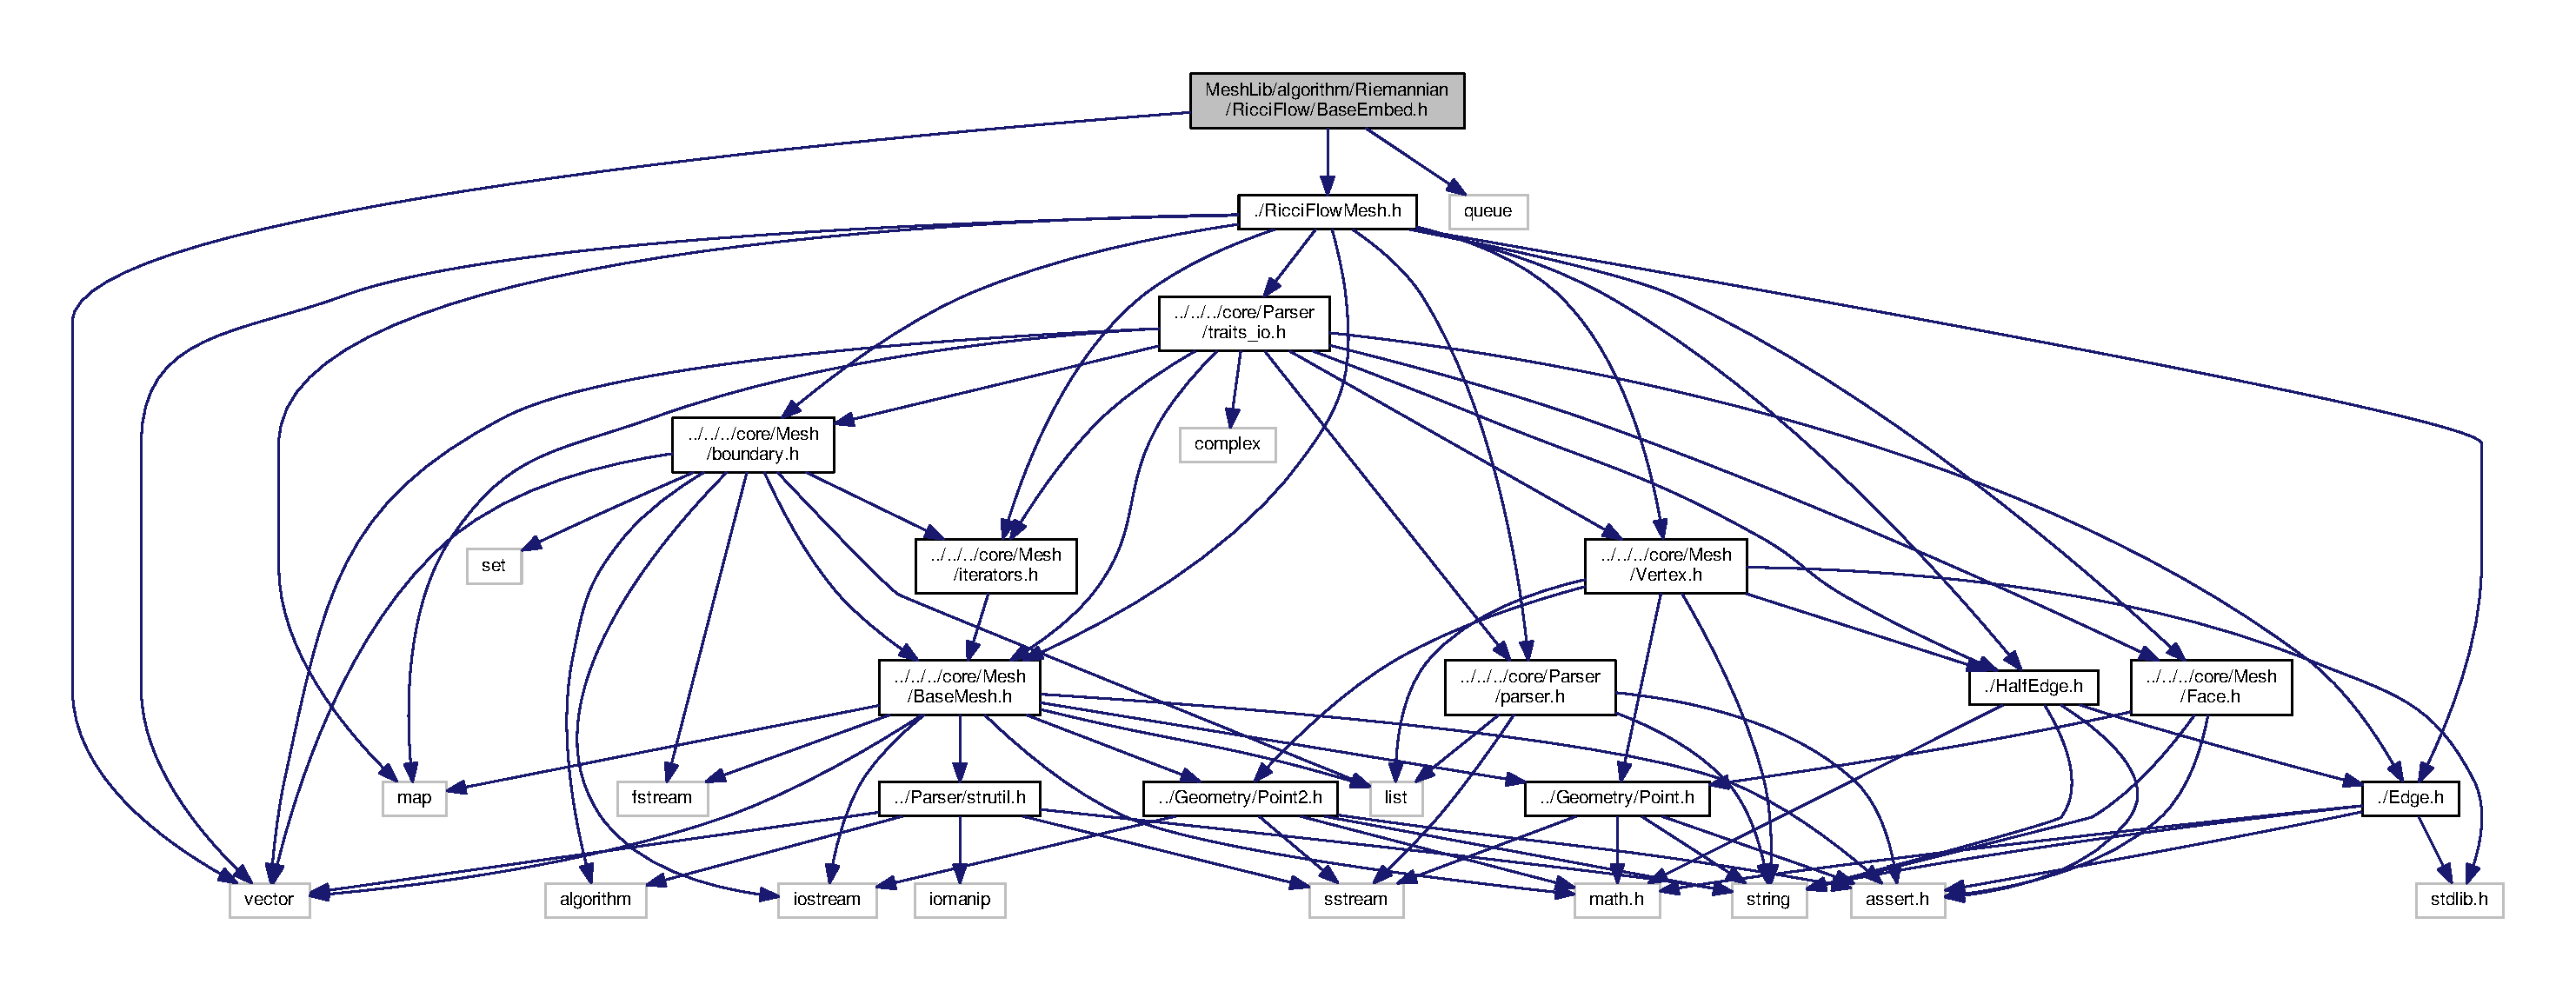
\includegraphics[width=350pt]{_base_embed_8h__incl}
\end{center}
\end{figure}
This graph shows which files directly or indirectly include this file\+:
\nopagebreak
\begin{figure}[H]
\begin{center}
\leavevmode
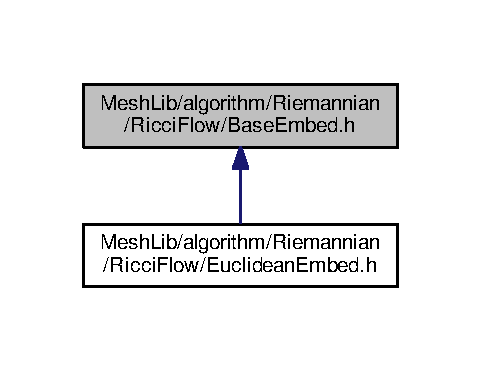
\includegraphics[width=231pt]{_base_embed_8h__dep__incl}
\end{center}
\end{figure}
\subsection*{Classes}
\begin{DoxyCompactItemize}
\item 
class \hyperlink{class_mesh_lib_1_1_c_base_embed}{Mesh\+Lib\+::\+C\+Base\+Embed$<$ C\+Vertex, C\+Edge, C\+Face, C\+Half\+Edge $>$}
\begin{DoxyCompactList}\small\item\em \hyperlink{class_mesh_lib_1_1_c_base_embed}{C\+Base\+Embed} class. \end{DoxyCompactList}\end{DoxyCompactItemize}
\subsection*{Namespaces}
\begin{DoxyCompactItemize}
\item 
 \hyperlink{namespace_mesh_lib}{Mesh\+Lib}
\end{DoxyCompactItemize}


\subsection{Detailed Description}
Isometrically embed a mesh with canonical metric onto the canonical domain. 

\begin{DoxyAuthor}{Author}
David Gu 
\end{DoxyAuthor}
\begin{DoxyDate}{Date}
documented on 10/17/2010
\end{DoxyDate}
Isometrically embed a mesh with canonical metric onto the canonical domain 
\hypertarget{_base_ricci_flow_8h}{}\section{Mesh\+Lib/algorithm/\+Riemannian/\+Ricci\+Flow/\+Base\+Ricci\+Flow.h File Reference}
\label{_base_ricci_flow_8h}\index{Mesh\+Lib/algorithm/\+Riemannian/\+Ricci\+Flow/\+Base\+Ricci\+Flow.\+h@{Mesh\+Lib/algorithm/\+Riemannian/\+Ricci\+Flow/\+Base\+Ricci\+Flow.\+h}}


Base class for Ricci flow algorithm.  


{\ttfamily \#include $<$map$>$}\\*
{\ttfamily \#include $<$vector$>$}\\*
{\ttfamily \#include $<$Eigen/\+Sparse$>$}\\*
{\ttfamily \#include \char`\"{}../../../core/\+Mesh/\+Base\+Mesh.\+h\char`\"{}}\\*
{\ttfamily \#include \char`\"{}../../../core/\+Mesh/\+Vertex.\+h\char`\"{}}\\*
{\ttfamily \#include \char`\"{}../../../core/\+Mesh/\+Half\+Edge.\+h\char`\"{}}\\*
{\ttfamily \#include \char`\"{}../../../core/\+Mesh/\+Edge.\+h\char`\"{}}\\*
{\ttfamily \#include \char`\"{}../../../core/\+Mesh/\+Face.\+h\char`\"{}}\\*
{\ttfamily \#include \char`\"{}../../../core/\+Mesh/iterators.\+h\char`\"{}}\\*
{\ttfamily \#include \char`\"{}../../../core/\+Mesh/boundary.\+h\char`\"{}}\\*
{\ttfamily \#include \char`\"{}../../../core/\+Parser/parser.\+h\char`\"{}}\\*
{\ttfamily \#include \char`\"{}./\+Ricci\+Flow\+Mesh.\+h\char`\"{}}\\*
This graph shows which files directly or indirectly include this file\+:
\nopagebreak
\begin{figure}[H]
\begin{center}
\leavevmode
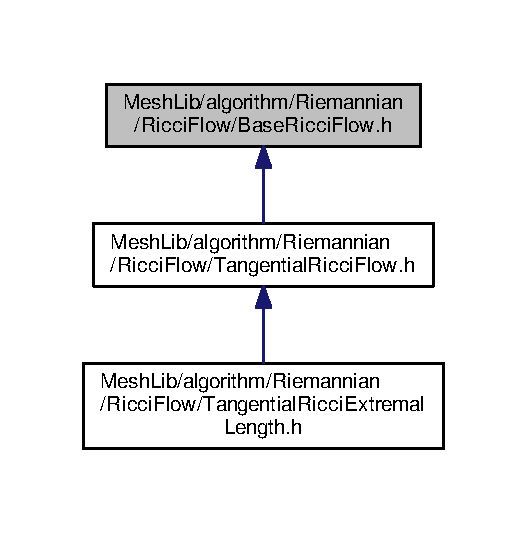
\includegraphics[width=253pt]{_base_ricci_flow_8h__dep__incl}
\end{center}
\end{figure}
\subsection*{Classes}
\begin{DoxyCompactItemize}
\item 
class \hyperlink{class_mesh_lib_1_1_c_base_ricci_flow}{Mesh\+Lib\+::\+C\+Base\+Ricci\+Flow$<$ V, E, F, H $>$}
\begin{DoxyCompactList}\small\item\em Base\+Class \hyperlink{class_mesh_lib_1_1_c_base_ricci_flow}{C\+Base\+Ricci\+Flow}. \end{DoxyCompactList}\end{DoxyCompactItemize}
\subsection*{Namespaces}
\begin{DoxyCompactItemize}
\item 
 \hyperlink{namespace_mesh_lib}{Mesh\+Lib}
\end{DoxyCompactItemize}
\subsection*{Macros}
\begin{DoxyCompactItemize}
\item 
\#define \hyperlink{_base_ricci_flow_8h_a598a3330b3c21701223ee0ca14316eca}{PI}~3.\+14159265358979323846
\end{DoxyCompactItemize}


\subsection{Detailed Description}
Base class for Ricci flow algorithm. 

\begin{DoxyAuthor}{Author}
David Gu 
\end{DoxyAuthor}
\begin{DoxyDate}{Date}
documented on 10/17/2010
\end{DoxyDate}
Algorithm for general Ricci Flow 

\subsection{Macro Definition Documentation}
\index{Base\+Ricci\+Flow.\+h@{Base\+Ricci\+Flow.\+h}!PI@{PI}}
\index{PI@{PI}!Base\+Ricci\+Flow.\+h@{Base\+Ricci\+Flow.\+h}}
\subsubsection[{\texorpdfstring{PI}{PI}}]{\setlength{\rightskip}{0pt plus 5cm}\#define PI~3.\+14159265358979323846}\hypertarget{_base_ricci_flow_8h_a598a3330b3c21701223ee0ca14316eca}{}\label{_base_ricci_flow_8h_a598a3330b3c21701223ee0ca14316eca}


Definition at line 27 of file Base\+Ricci\+Flow.\+h.


\hypertarget{_euclidean_embed_8h}{}\section{Mesh\+Lib/algorithm/\+Riemannian/\+Ricci\+Flow/\+Euclidean\+Embed.h File Reference}
\label{_euclidean_embed_8h}\index{Mesh\+Lib/algorithm/\+Riemannian/\+Ricci\+Flow/\+Euclidean\+Embed.\+h@{Mesh\+Lib/algorithm/\+Riemannian/\+Ricci\+Flow/\+Euclidean\+Embed.\+h}}


Isometrically embed a mesh with flat metric onto the plane.  


{\ttfamily \#include $<$vector$>$}\\*
{\ttfamily \#include $<$queue$>$}\\*
{\ttfamily \#include \char`\"{}./\+Ricci\+Flow\+Mesh.\+h\char`\"{}}\\*
{\ttfamily \#include \char`\"{}./\+Base\+Embed.\+h\char`\"{}}\\*
{\ttfamily \#include \char`\"{}../../../core/\+Geometry/\+Circle.\+h\char`\"{}}\\*
Include dependency graph for Euclidean\+Embed.\+h\+:
\nopagebreak
\begin{figure}[H]
\begin{center}
\leavevmode
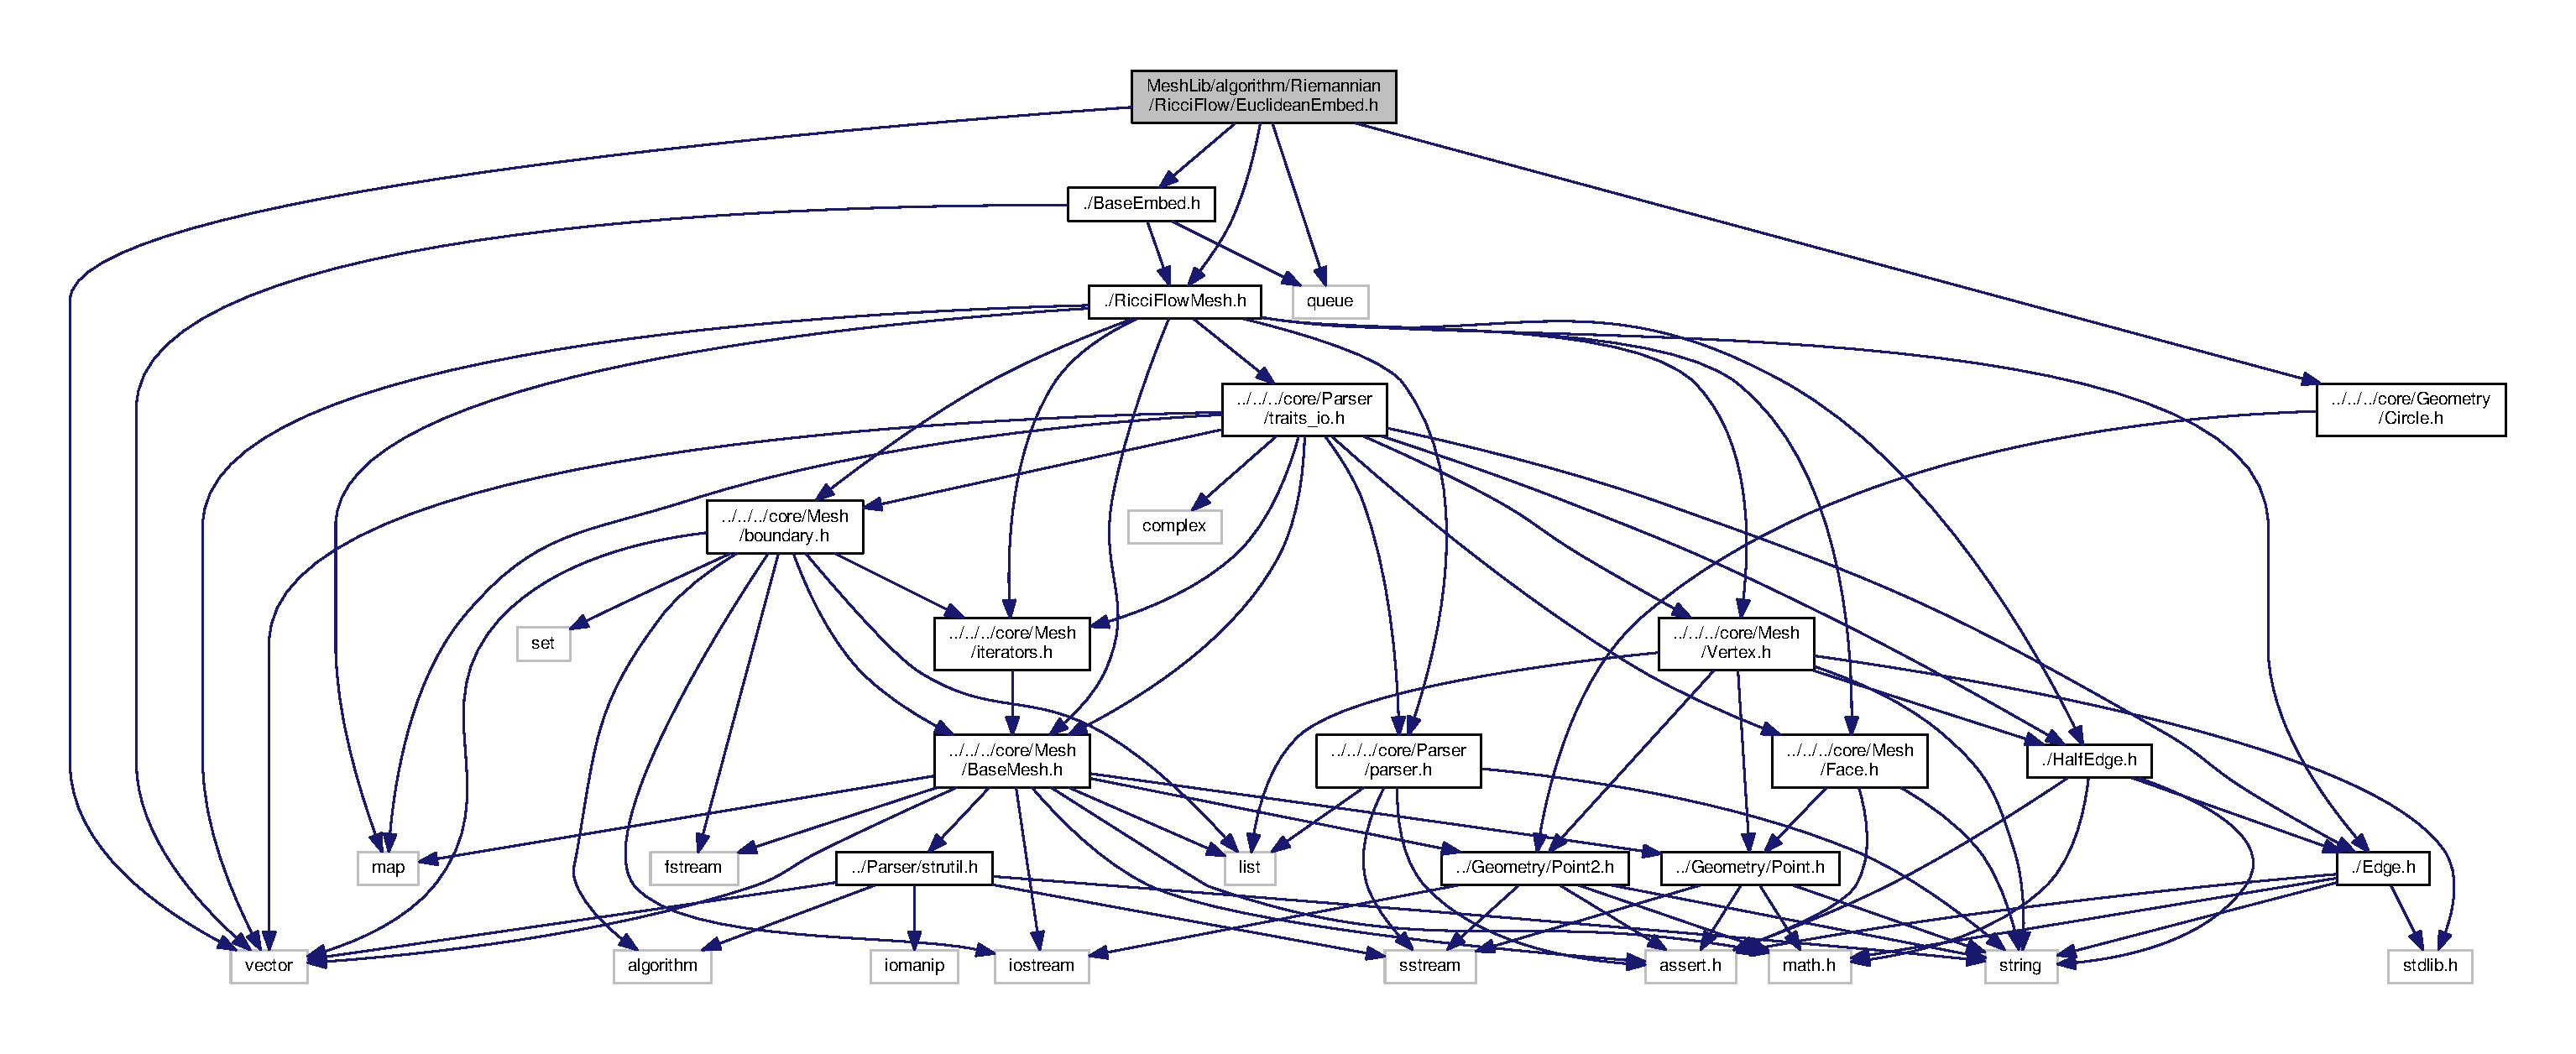
\includegraphics[width=350pt]{_euclidean_embed_8h__incl}
\end{center}
\end{figure}
\subsection*{Classes}
\begin{DoxyCompactItemize}
\item 
class \hyperlink{class_mesh_lib_1_1_c_euclidean_embed}{Mesh\+Lib\+::\+C\+Euclidean\+Embed$<$ C\+Vertex, C\+Edge, C\+Face, C\+Half\+Edge $>$}
\begin{DoxyCompactList}\small\item\em C\+Embed class. \end{DoxyCompactList}\end{DoxyCompactItemize}
\subsection*{Namespaces}
\begin{DoxyCompactItemize}
\item 
 \hyperlink{namespace_mesh_lib}{Mesh\+Lib}
\end{DoxyCompactItemize}
\subsection*{Typedefs}
\begin{DoxyCompactItemize}
\item 
typedef C\+Euclidean\+Embed$<$ C\+Ricci\+Flow\+Vertex, C\+Ricci\+Flow\+Edge, C\+Ricci\+Flow\+Face, C\+Ricci\+Flow\+Half\+Edge $>$ \hyperlink{namespace_mesh_lib_abdc9df09977d6c620bf5be5a4af503c5}{Mesh\+Lib\+::\+C\+R\+F\+Embed}
\end{DoxyCompactItemize}


\subsection{Detailed Description}
Isometrically embed a mesh with flat metric onto the plane. 

\begin{DoxyAuthor}{Author}
David Gu 
\end{DoxyAuthor}
\begin{DoxyDate}{Date}
documented on 10/17/2010
\end{DoxyDate}
Embed a mesh with flat metric on canonical domain 
\hypertarget{_ricci_flow_mesh_8h}{}\section{Mesh\+Lib/algorithm/\+Riemannian/\+Ricci\+Flow/\+Ricci\+Flow\+Mesh.h File Reference}
\label{_ricci_flow_mesh_8h}\index{Mesh\+Lib/algorithm/\+Riemannian/\+Ricci\+Flow/\+Ricci\+Flow\+Mesh.\+h@{Mesh\+Lib/algorithm/\+Riemannian/\+Ricci\+Flow/\+Ricci\+Flow\+Mesh.\+h}}


Mesh for Ricci Flow.  


{\ttfamily \#include $<$map$>$}\\*
{\ttfamily \#include $<$vector$>$}\\*
{\ttfamily \#include \char`\"{}../../../core/\+Mesh/\+Base\+Mesh.\+h\char`\"{}}\\*
{\ttfamily \#include \char`\"{}../../../core/\+Mesh/\+Vertex.\+h\char`\"{}}\\*
{\ttfamily \#include \char`\"{}../../../core/\+Mesh/\+Half\+Edge.\+h\char`\"{}}\\*
{\ttfamily \#include \char`\"{}../../../core/\+Mesh/\+Edge.\+h\char`\"{}}\\*
{\ttfamily \#include \char`\"{}../../../core/\+Mesh/\+Face.\+h\char`\"{}}\\*
{\ttfamily \#include \char`\"{}../../../core/\+Mesh/iterators.\+h\char`\"{}}\\*
{\ttfamily \#include \char`\"{}../../../core/\+Mesh/boundary.\+h\char`\"{}}\\*
{\ttfamily \#include \char`\"{}../../../core/\+Parser/parser.\+h\char`\"{}}\\*
{\ttfamily \#include \char`\"{}../../../core/\+Parser/traits\+\_\+io.\+h\char`\"{}}\\*
Include dependency graph for Ricci\+Flow\+Mesh.\+h\+:
\nopagebreak
\begin{figure}[H]
\begin{center}
\leavevmode
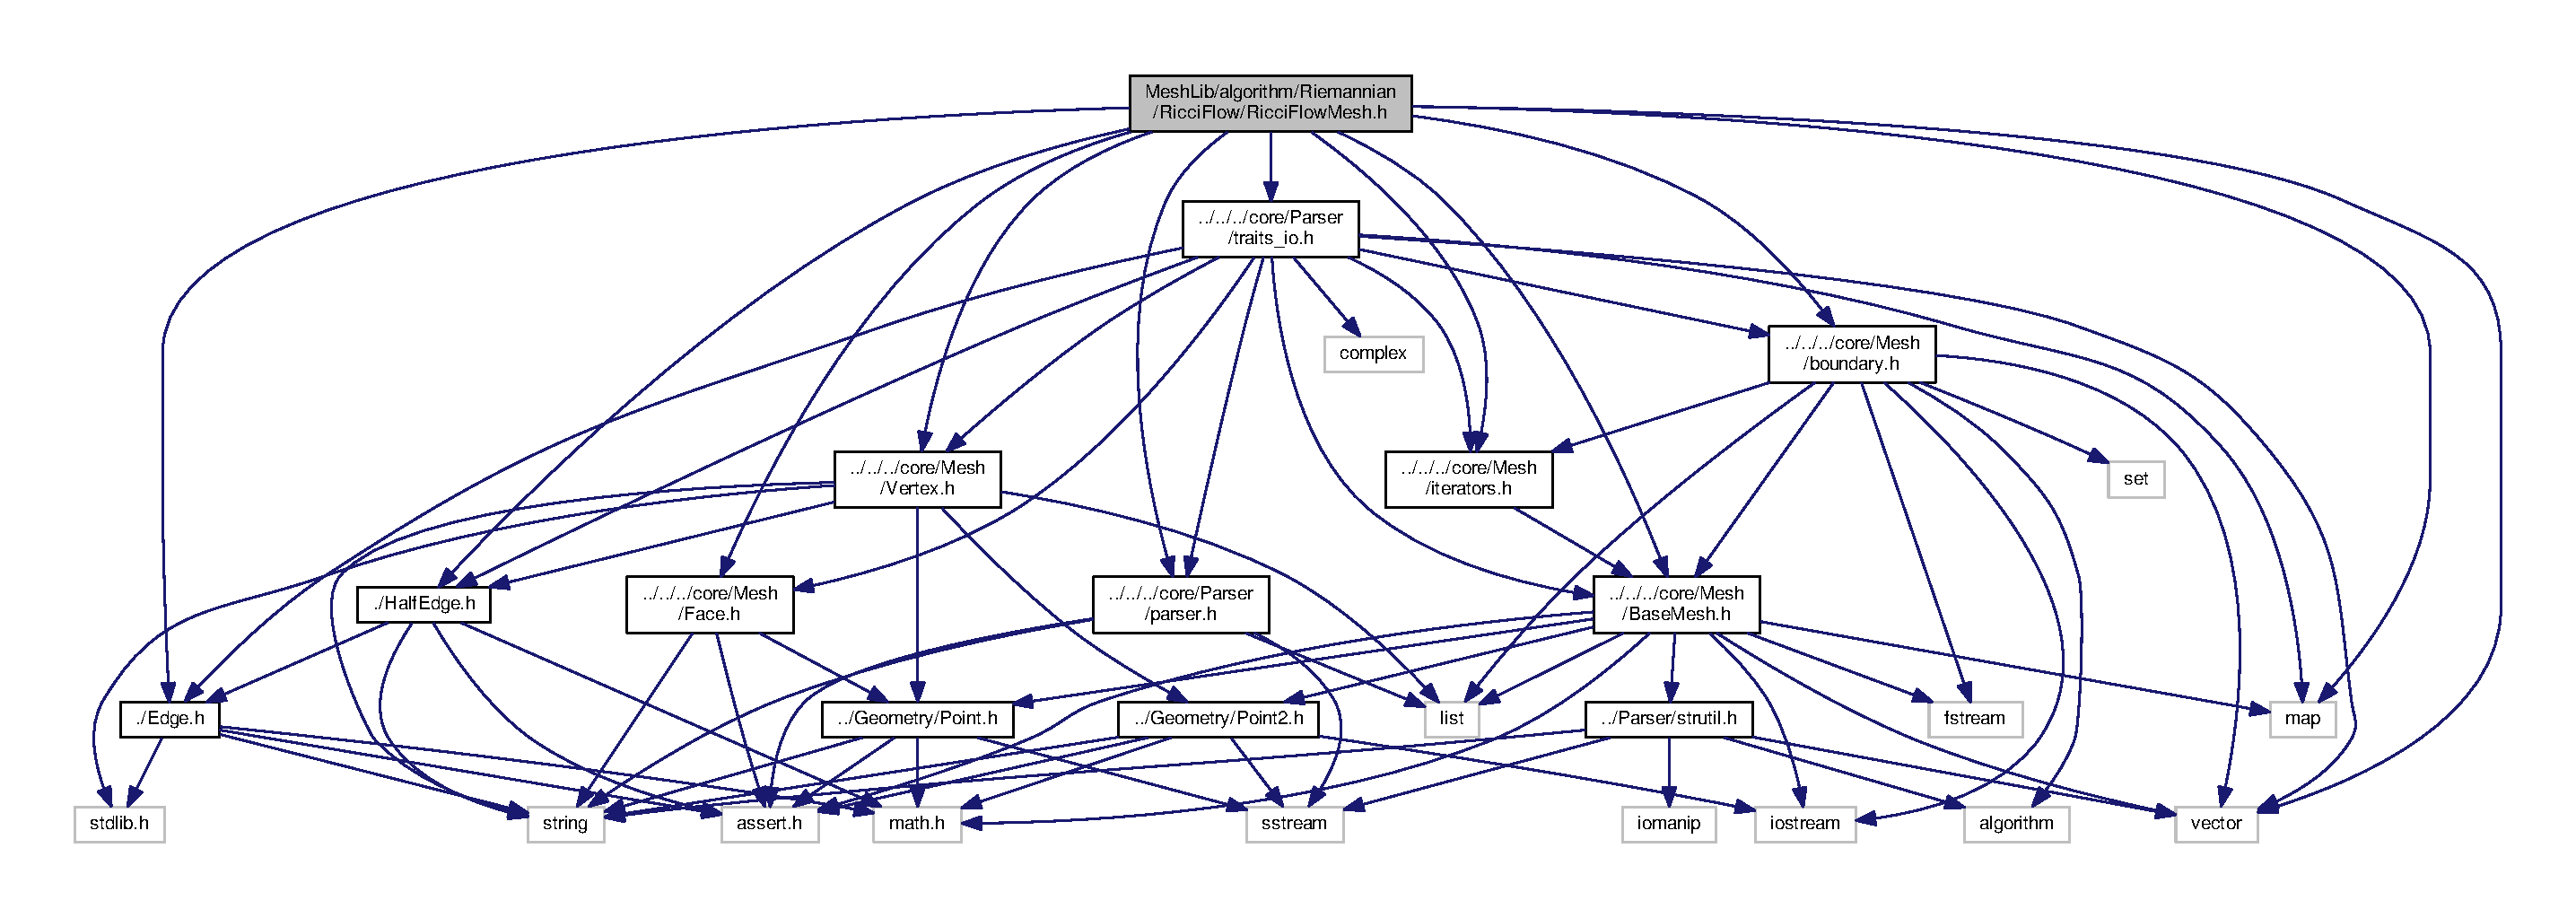
\includegraphics[width=350pt]{_ricci_flow_mesh_8h__incl}
\end{center}
\end{figure}
This graph shows which files directly or indirectly include this file\+:
\nopagebreak
\begin{figure}[H]
\begin{center}
\leavevmode
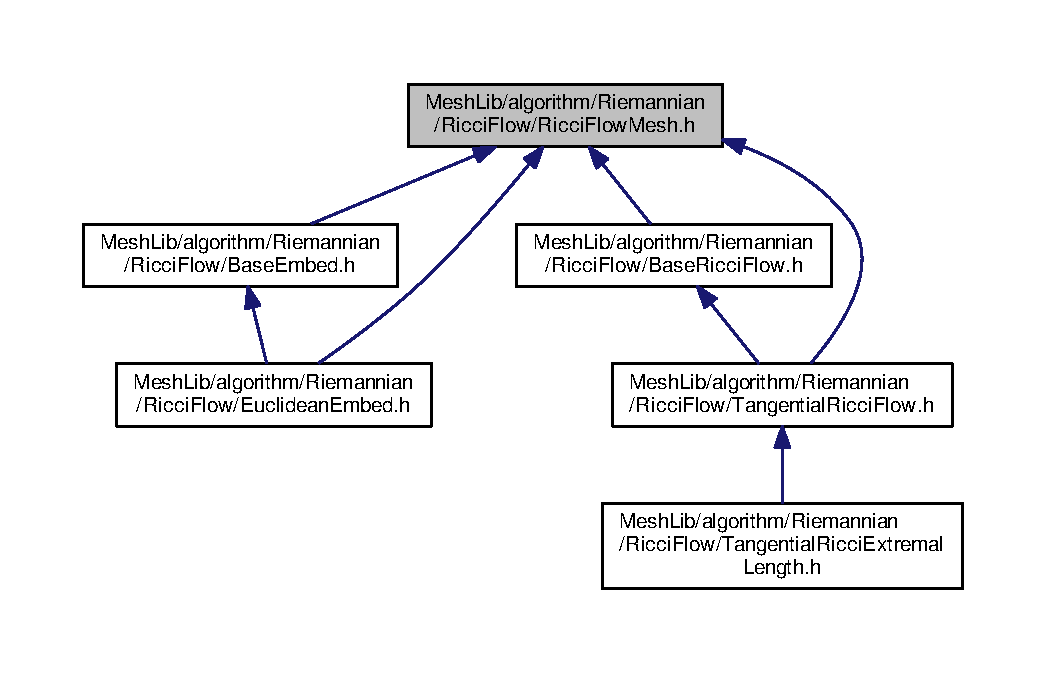
\includegraphics[width=350pt]{_ricci_flow_mesh_8h__dep__incl}
\end{center}
\end{figure}
\subsection*{Classes}
\begin{DoxyCompactItemize}
\item 
class \hyperlink{class_mesh_lib_1_1_c_ricci_flow_vertex}{Mesh\+Lib\+::\+C\+Ricci\+Flow\+Vertex}
\begin{DoxyCompactList}\small\item\em \hyperlink{class_mesh_lib_1_1_c_ricci_flow_vertex}{C\+Ricci\+Flow\+Vertex} class. \end{DoxyCompactList}\end{DoxyCompactItemize}
\subsection*{Namespaces}
\begin{DoxyCompactItemize}
\item 
 \hyperlink{namespace_mesh_lib}{Mesh\+Lib}
\end{DoxyCompactItemize}
\subsection*{Macros}
\begin{DoxyCompactItemize}
\item 
\#define \hyperlink{_ricci_flow_mesh_8h_a0bfde98079098c03a7d9144f18454789}{T\+R\+A\+IT}~N\+O\+R\+M\+AL  1
\item 
\#define \hyperlink{_ricci_flow_mesh_8h_a956e39330f16fa0ea011c6c52610ea6e}{T\+R\+A\+I\+T\+\_\+\+F\+A\+T\+H\+ER}~2
\item 
\#define \hyperlink{_ricci_flow_mesh_8h_a32c2b9ea91ba20adf157bcda05cdc9f9}{T\+R\+A\+I\+T\+\_\+\+UV}~4
\item 
\#define \hyperlink{_ricci_flow_mesh_8h_a552257d596051c7eddec3452bd1d253d}{T\+R\+A\+I\+T\+\_\+\+R\+GB}~8
\item 
\#define \hyperlink{_ricci_flow_mesh_8h_a31427dab3ff67a8cb90e8792b728dd5d}{T\+R\+A\+I\+T\+\_\+\+P\+A\+R\+E\+NT}~16
\end{DoxyCompactItemize}
\subsection*{Functions}
\begin{DoxyCompactItemize}
\item 
double \& \hyperlink{namespace_mesh_lib_a7c52b467ab87ddda5e6fe7b6d0a25148}{Mesh\+Lib\+::dtheta\+\_\+du} ()
\begin{DoxyCompactList}\small\item\em C\+Ricci\+Flow\+Edge class. \end{DoxyCompactList}\end{DoxyCompactItemize}


\subsection{Detailed Description}
Mesh for Ricci Flow. 

\begin{DoxyAuthor}{Author}
David Gu 
\end{DoxyAuthor}
\begin{DoxyDate}{Date}
Documented 10/16/2010 
\end{DoxyDate}


\subsection{Macro Definition Documentation}
\index{Ricci\+Flow\+Mesh.\+h@{Ricci\+Flow\+Mesh.\+h}!T\+R\+A\+IT@{T\+R\+A\+IT}}
\index{T\+R\+A\+IT@{T\+R\+A\+IT}!Ricci\+Flow\+Mesh.\+h@{Ricci\+Flow\+Mesh.\+h}}
\subsubsection[{\texorpdfstring{T\+R\+A\+IT}{TRAIT}}]{\setlength{\rightskip}{0pt plus 5cm}\#define T\+R\+A\+IT~N\+O\+R\+M\+AL  1}\hypertarget{_ricci_flow_mesh_8h_a0bfde98079098c03a7d9144f18454789}{}\label{_ricci_flow_mesh_8h_a0bfde98079098c03a7d9144f18454789}


Definition at line 28 of file Ricci\+Flow\+Mesh.\+h.

\index{Ricci\+Flow\+Mesh.\+h@{Ricci\+Flow\+Mesh.\+h}!T\+R\+A\+I\+T\+\_\+\+F\+A\+T\+H\+ER@{T\+R\+A\+I\+T\+\_\+\+F\+A\+T\+H\+ER}}
\index{T\+R\+A\+I\+T\+\_\+\+F\+A\+T\+H\+ER@{T\+R\+A\+I\+T\+\_\+\+F\+A\+T\+H\+ER}!Ricci\+Flow\+Mesh.\+h@{Ricci\+Flow\+Mesh.\+h}}
\subsubsection[{\texorpdfstring{T\+R\+A\+I\+T\+\_\+\+F\+A\+T\+H\+ER}{TRAIT_FATHER}}]{\setlength{\rightskip}{0pt plus 5cm}\#define T\+R\+A\+I\+T\+\_\+\+F\+A\+T\+H\+ER~2}\hypertarget{_ricci_flow_mesh_8h_a956e39330f16fa0ea011c6c52610ea6e}{}\label{_ricci_flow_mesh_8h_a956e39330f16fa0ea011c6c52610ea6e}


Definition at line 29 of file Ricci\+Flow\+Mesh.\+h.

\index{Ricci\+Flow\+Mesh.\+h@{Ricci\+Flow\+Mesh.\+h}!T\+R\+A\+I\+T\+\_\+\+P\+A\+R\+E\+NT@{T\+R\+A\+I\+T\+\_\+\+P\+A\+R\+E\+NT}}
\index{T\+R\+A\+I\+T\+\_\+\+P\+A\+R\+E\+NT@{T\+R\+A\+I\+T\+\_\+\+P\+A\+R\+E\+NT}!Ricci\+Flow\+Mesh.\+h@{Ricci\+Flow\+Mesh.\+h}}
\subsubsection[{\texorpdfstring{T\+R\+A\+I\+T\+\_\+\+P\+A\+R\+E\+NT}{TRAIT_PARENT}}]{\setlength{\rightskip}{0pt plus 5cm}\#define T\+R\+A\+I\+T\+\_\+\+P\+A\+R\+E\+NT~16}\hypertarget{_ricci_flow_mesh_8h_a31427dab3ff67a8cb90e8792b728dd5d}{}\label{_ricci_flow_mesh_8h_a31427dab3ff67a8cb90e8792b728dd5d}


Definition at line 32 of file Ricci\+Flow\+Mesh.\+h.

\index{Ricci\+Flow\+Mesh.\+h@{Ricci\+Flow\+Mesh.\+h}!T\+R\+A\+I\+T\+\_\+\+R\+GB@{T\+R\+A\+I\+T\+\_\+\+R\+GB}}
\index{T\+R\+A\+I\+T\+\_\+\+R\+GB@{T\+R\+A\+I\+T\+\_\+\+R\+GB}!Ricci\+Flow\+Mesh.\+h@{Ricci\+Flow\+Mesh.\+h}}
\subsubsection[{\texorpdfstring{T\+R\+A\+I\+T\+\_\+\+R\+GB}{TRAIT_RGB}}]{\setlength{\rightskip}{0pt plus 5cm}\#define T\+R\+A\+I\+T\+\_\+\+R\+GB~8}\hypertarget{_ricci_flow_mesh_8h_a552257d596051c7eddec3452bd1d253d}{}\label{_ricci_flow_mesh_8h_a552257d596051c7eddec3452bd1d253d}


Definition at line 31 of file Ricci\+Flow\+Mesh.\+h.

\index{Ricci\+Flow\+Mesh.\+h@{Ricci\+Flow\+Mesh.\+h}!T\+R\+A\+I\+T\+\_\+\+UV@{T\+R\+A\+I\+T\+\_\+\+UV}}
\index{T\+R\+A\+I\+T\+\_\+\+UV@{T\+R\+A\+I\+T\+\_\+\+UV}!Ricci\+Flow\+Mesh.\+h@{Ricci\+Flow\+Mesh.\+h}}
\subsubsection[{\texorpdfstring{T\+R\+A\+I\+T\+\_\+\+UV}{TRAIT_UV}}]{\setlength{\rightskip}{0pt plus 5cm}\#define T\+R\+A\+I\+T\+\_\+\+UV~4}\hypertarget{_ricci_flow_mesh_8h_a32c2b9ea91ba20adf157bcda05cdc9f9}{}\label{_ricci_flow_mesh_8h_a32c2b9ea91ba20adf157bcda05cdc9f9}


Definition at line 30 of file Ricci\+Flow\+Mesh.\+h.


\hypertarget{_tangential_ricci_extremal_length_8h}{}\section{Mesh\+Lib/algorithm/\+Riemannian/\+Ricci\+Flow/\+Tangential\+Ricci\+Extremal\+Length.h File Reference}
\label{_tangential_ricci_extremal_length_8h}\index{Mesh\+Lib/algorithm/\+Riemannian/\+Ricci\+Flow/\+Tangential\+Ricci\+Extremal\+Length.\+h@{Mesh\+Lib/algorithm/\+Riemannian/\+Ricci\+Flow/\+Tangential\+Ricci\+Extremal\+Length.\+h}}


Euclidean Tangential Ricci flow for Extremal Length.  


{\ttfamily \#include $<$map$>$}\\*
{\ttfamily \#include $<$vector$>$}\\*
{\ttfamily \#include \char`\"{}./\+Tangential\+Ricci\+Flow.\+h\char`\"{}}\\*
Include dependency graph for Tangential\+Ricci\+Extremal\+Length.\+h\+:
\nopagebreak
\begin{figure}[H]
\begin{center}
\leavevmode
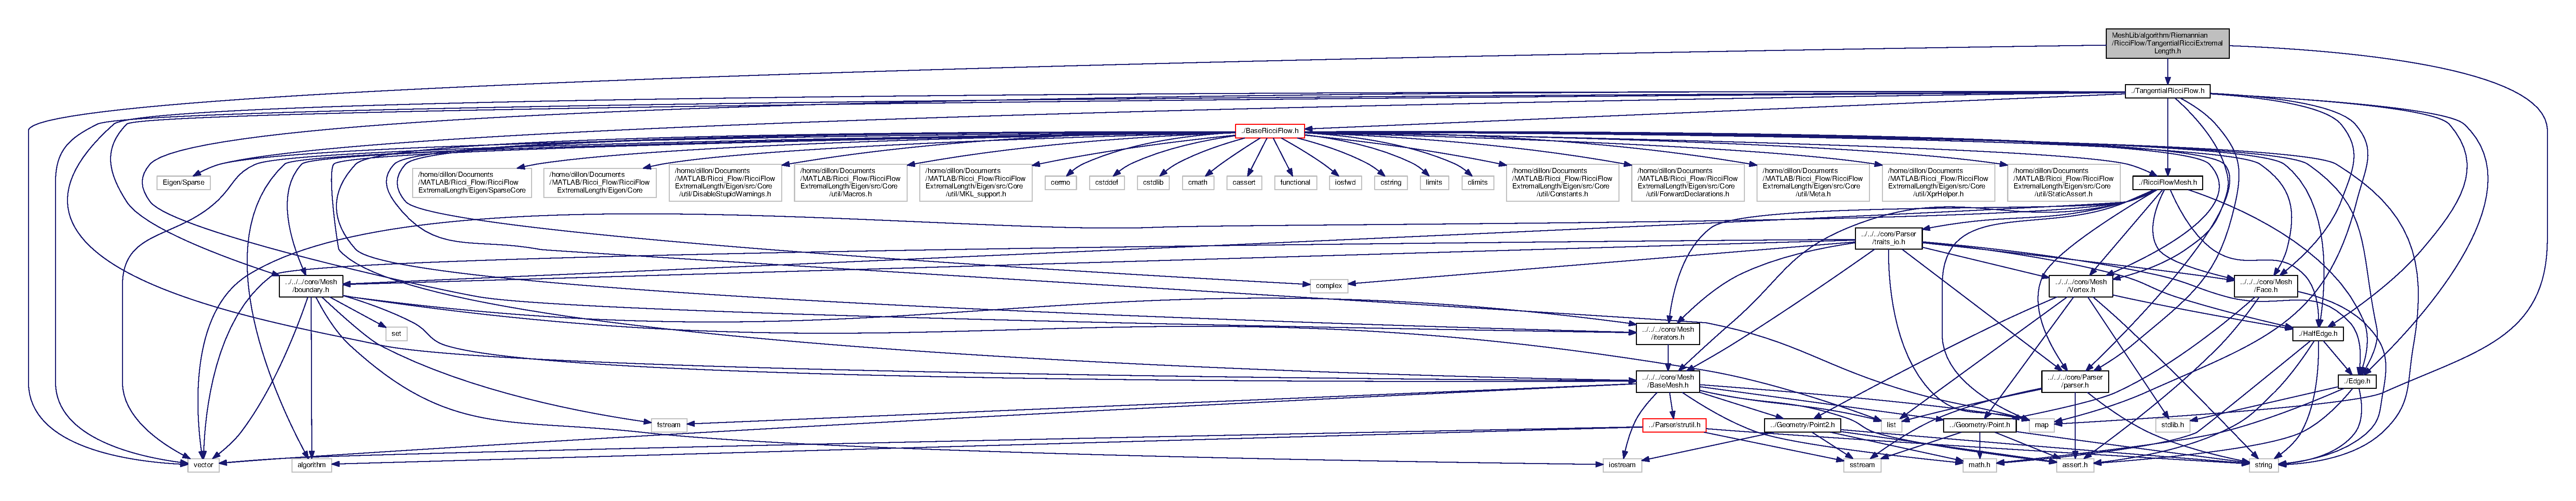
\includegraphics[width=350pt]{_tangential_ricci_extremal_length_8h__incl}
\end{center}
\end{figure}
\subsection*{Classes}
\begin{DoxyCompactItemize}
\item 
class \hyperlink{class_mesh_lib_1_1_c_tangential_ricci_flow_extremal_length}{Mesh\+Lib\+::\+C\+Tangential\+Ricci\+Flow\+Extremal\+Length$<$ V, E, F, H $>$}
\begin{DoxyCompactList}\small\item\em C\+Inversive\+Distance\+Ricci\+Flow\+Extremal\+Length class. \end{DoxyCompactList}\end{DoxyCompactItemize}
\subsection*{Namespaces}
\begin{DoxyCompactItemize}
\item 
 \hyperlink{namespace_mesh_lib}{Mesh\+Lib}
\end{DoxyCompactItemize}


\subsection{Detailed Description}
Euclidean Tangential Ricci flow for Extremal Length. 

\begin{DoxyAuthor}{Author}
David Gu 
\end{DoxyAuthor}
\begin{DoxyDate}{Date}
documented on 11/15/2010
\end{DoxyDate}
Algorithm for Tangential Ricci Flow for Extremal Length 
\hypertarget{_tangential_ricci_flow_8h}{}\section{Mesh\+Lib/algorithm/\+Riemannian/\+Ricci\+Flow/\+Tangential\+Ricci\+Flow.h File Reference}
\label{_tangential_ricci_flow_8h}\index{Mesh\+Lib/algorithm/\+Riemannian/\+Ricci\+Flow/\+Tangential\+Ricci\+Flow.\+h@{Mesh\+Lib/algorithm/\+Riemannian/\+Ricci\+Flow/\+Tangential\+Ricci\+Flow.\+h}}


General Euclidean Ricci flow algorithm.  


{\ttfamily \#include $<$map$>$}\\*
{\ttfamily \#include $<$vector$>$}\\*
{\ttfamily \#include $<$Eigen/\+Sparse$>$}\\*
{\ttfamily \#include \char`\"{}../../../core/\+Mesh/\+Base\+Mesh.\+h\char`\"{}}\\*
{\ttfamily \#include \char`\"{}../../../core/\+Mesh/\+Vertex.\+h\char`\"{}}\\*
{\ttfamily \#include \char`\"{}../../../core/\+Mesh/\+Half\+Edge.\+h\char`\"{}}\\*
{\ttfamily \#include \char`\"{}../../../core/\+Mesh/\+Edge.\+h\char`\"{}}\\*
{\ttfamily \#include \char`\"{}../../../core/\+Mesh/\+Face.\+h\char`\"{}}\\*
{\ttfamily \#include \char`\"{}../../../core/\+Mesh/iterators.\+h\char`\"{}}\\*
{\ttfamily \#include \char`\"{}../../../core/\+Mesh/boundary.\+h\char`\"{}}\\*
{\ttfamily \#include \char`\"{}../../../core/\+Parser/parser.\+h\char`\"{}}\\*
{\ttfamily \#include \char`\"{}./\+Ricci\+Flow\+Mesh.\+h\char`\"{}}\\*
{\ttfamily \#include \char`\"{}./\+Base\+Ricci\+Flow.\+h\char`\"{}}\\*
Include dependency graph for Tangential\+Ricci\+Flow.\+h\+:
\nopagebreak
\begin{figure}[H]
\begin{center}
\leavevmode
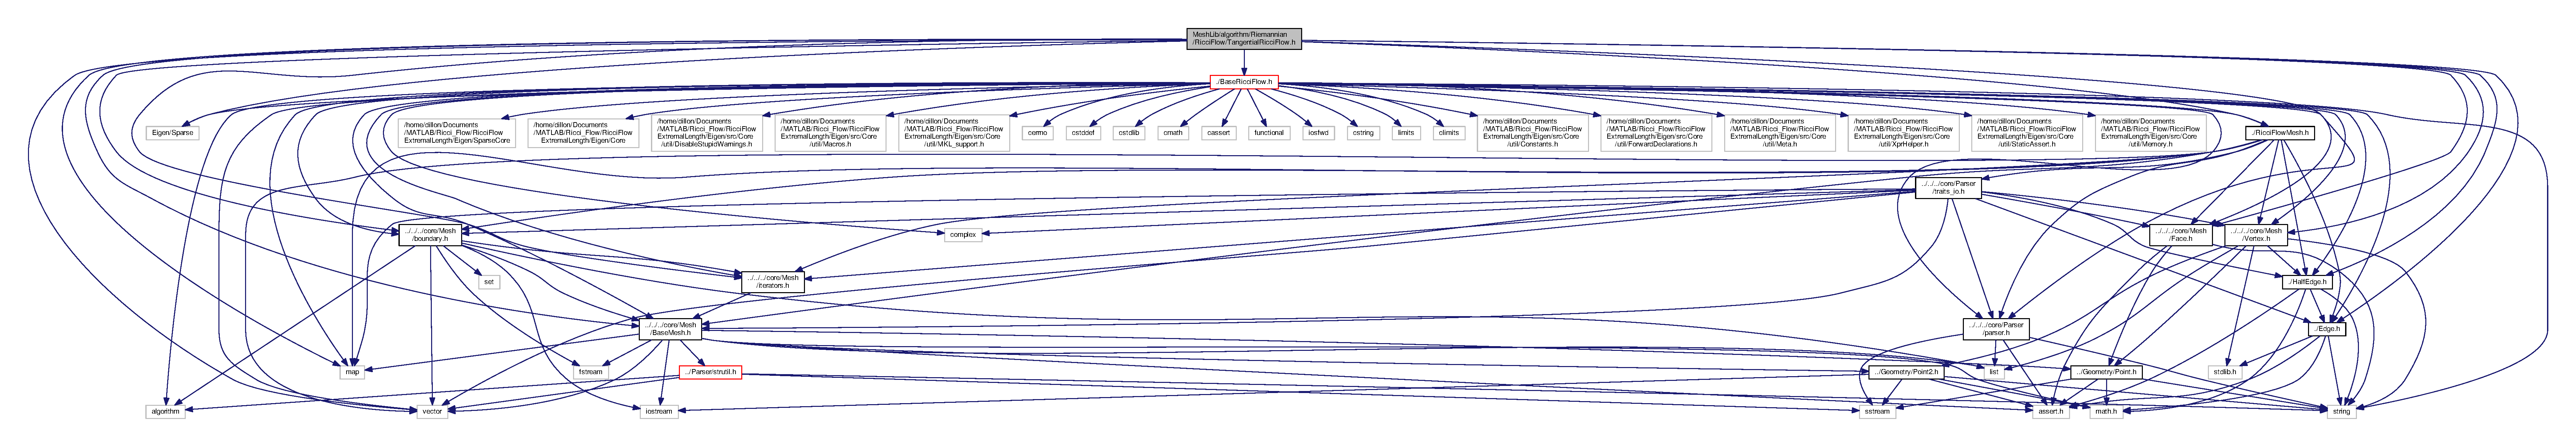
\includegraphics[width=350pt]{_tangential_ricci_flow_8h__incl}
\end{center}
\end{figure}
This graph shows which files directly or indirectly include this file\+:
\nopagebreak
\begin{figure}[H]
\begin{center}
\leavevmode
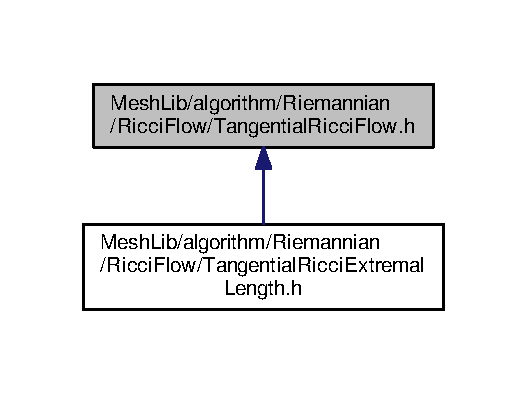
\includegraphics[width=253pt]{_tangential_ricci_flow_8h__dep__incl}
\end{center}
\end{figure}
\subsection*{Classes}
\begin{DoxyCompactItemize}
\item 
class \hyperlink{class_mesh_lib_1_1_c_tangential_ricci_flow}{Mesh\+Lib\+::\+C\+Tangential\+Ricci\+Flow$<$ V, E, F, H $>$}
\begin{DoxyCompactList}\small\item\em Class \hyperlink{class_mesh_lib_1_1_c_tangential_ricci_flow}{C\+Tangential\+Ricci\+Flow}. \end{DoxyCompactList}\end{DoxyCompactItemize}
\subsection*{Namespaces}
\begin{DoxyCompactItemize}
\item 
 \hyperlink{namespace_mesh_lib}{Mesh\+Lib}
\end{DoxyCompactItemize}


\subsection{Detailed Description}
General Euclidean Ricci flow algorithm. 

\begin{DoxyAuthor}{Author}
David Gu 
\end{DoxyAuthor}
\begin{DoxyDate}{Date}
documented on 10/17/2010
\end{DoxyDate}
Algorithm for general Ricci Flow 
\hypertarget{_structure_8h}{}\section{Mesh\+Lib/algorithm/\+Structure/\+Structure.h File Reference}
\label{_structure_8h}\index{Mesh\+Lib/algorithm/\+Structure/\+Structure.\+h@{Mesh\+Lib/algorithm/\+Structure/\+Structure.\+h}}


algorithms for converting one structure to another  


{\ttfamily \#include $<$map$>$}\\*
{\ttfamily \#include $<$vector$>$}\\*
{\ttfamily \#include $<$complex$>$}\\*
{\ttfamily \#include \char`\"{}../../core/\+Mesh/\+Base\+Mesh.\+h\char`\"{}}\\*
{\ttfamily \#include \char`\"{}../../core/\+Mesh/\+Vertex.\+h\char`\"{}}\\*
{\ttfamily \#include \char`\"{}../../core/\+Mesh/\+Half\+Edge.\+h\char`\"{}}\\*
{\ttfamily \#include \char`\"{}../../core/\+Mesh/\+Edge.\+h\char`\"{}}\\*
{\ttfamily \#include \char`\"{}../../core/\+Mesh/\+Face.\+h\char`\"{}}\\*
{\ttfamily \#include \char`\"{}../../core/\+Mesh/iterators.\+h\char`\"{}}\\*
{\ttfamily \#include \char`\"{}../../core/\+Mesh/boundary.\+h\char`\"{}}\\*
{\ttfamily \#include \char`\"{}../../core/\+Parser/parser.\+h\char`\"{}}\\*
Include dependency graph for Structure.\+h\+:
\nopagebreak
\begin{figure}[H]
\begin{center}
\leavevmode
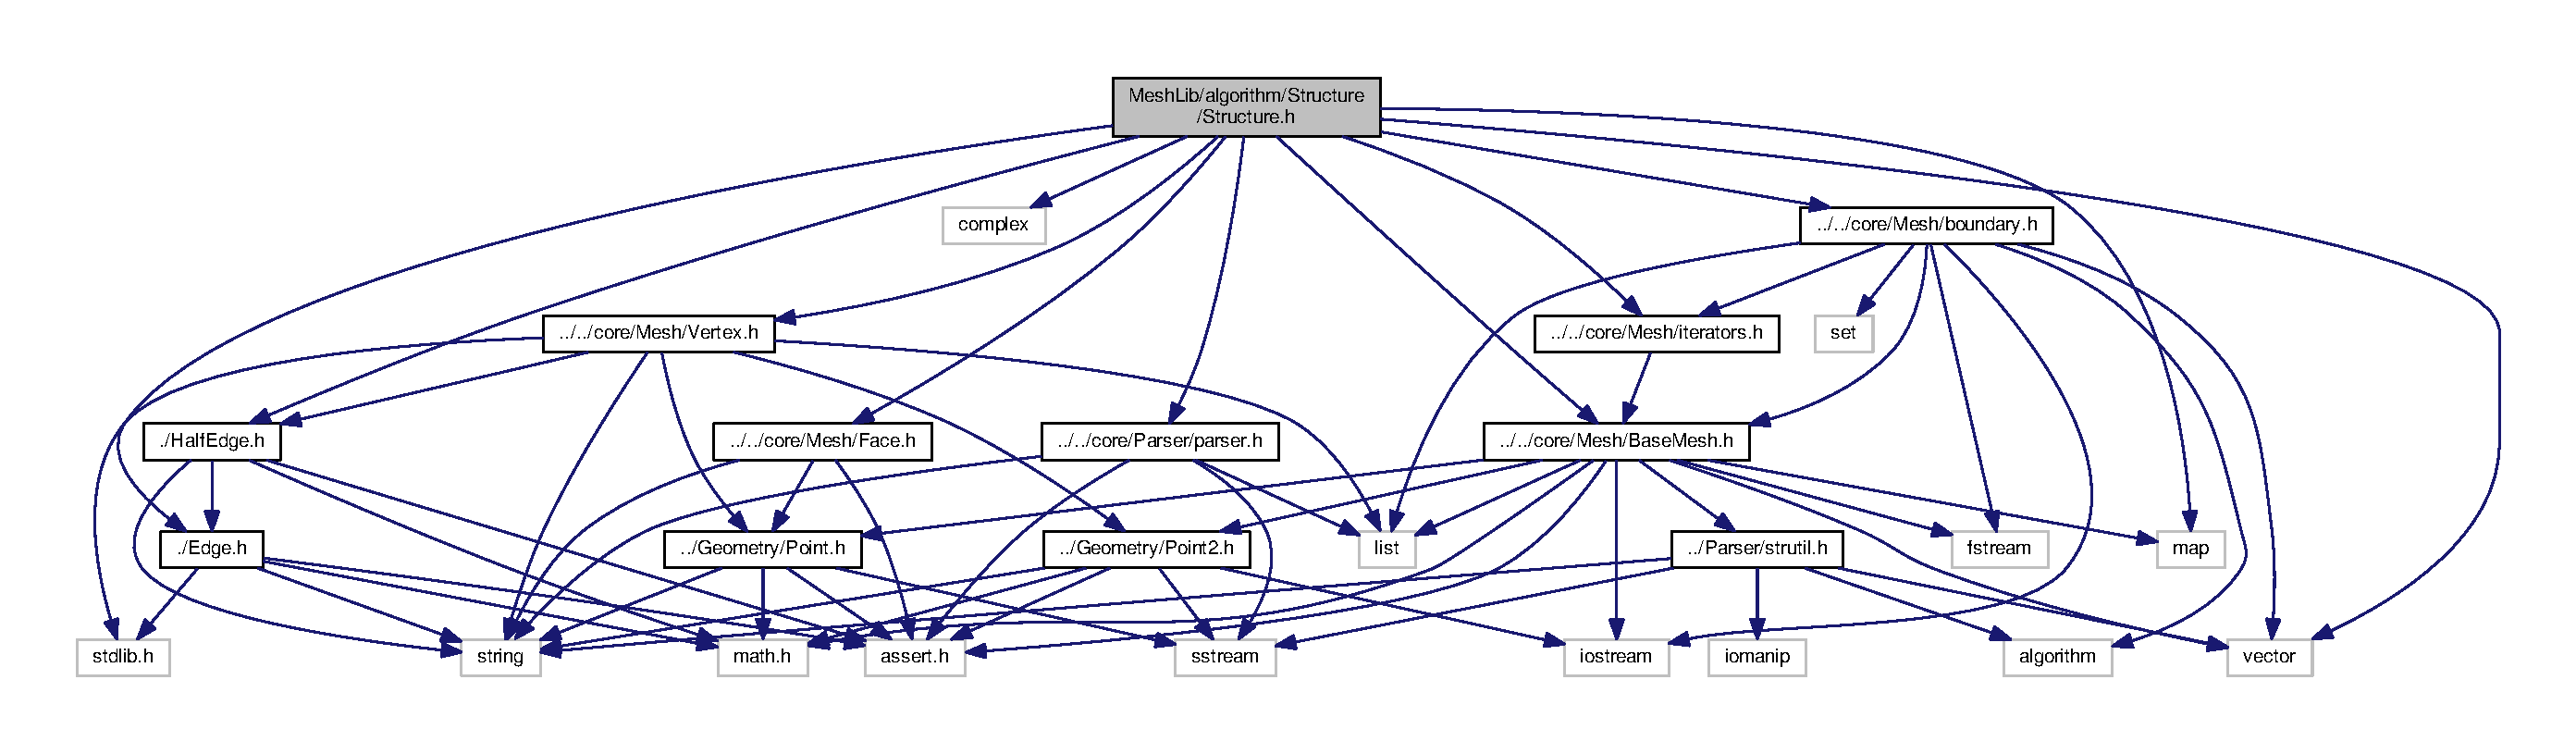
\includegraphics[width=350pt]{_structure_8h__incl}
\end{center}
\end{figure}
\subsection*{Classes}
\begin{DoxyCompactItemize}
\item 
class \hyperlink{class_mesh_lib_1_1_c_structure}{Mesh\+Lib\+::\+C\+Structure$<$ Mesh, V, E, F, H $>$}
\begin{DoxyCompactList}\small\item\em Conversion class. \end{DoxyCompactList}\end{DoxyCompactItemize}
\subsection*{Namespaces}
\begin{DoxyCompactItemize}
\item 
 \hyperlink{namespace_mesh_lib}{Mesh\+Lib}
\end{DoxyCompactItemize}
\subsection*{Macros}
\begin{DoxyCompactItemize}
\item 
\#define \hyperlink{_structure_8h_a598a3330b3c21701223ee0ca14316eca}{PI}~3.\+14159265358979323846
\end{DoxyCompactItemize}


\subsection{Detailed Description}
algorithms for converting one structure to another 

\begin{DoxyAuthor}{Author}
David Gu 
\end{DoxyAuthor}
\begin{DoxyDate}{Date}
documented on 5/6/2011
\end{DoxyDate}
Algorithm for structure conversions 

\subsection{Macro Definition Documentation}
\index{Structure.\+h@{Structure.\+h}!PI@{PI}}
\index{PI@{PI}!Structure.\+h@{Structure.\+h}}
\subsubsection[{\texorpdfstring{PI}{PI}}]{\setlength{\rightskip}{0pt plus 5cm}\#define PI~3.\+14159265358979323846}\hypertarget{_structure_8h_a598a3330b3c21701223ee0ca14316eca}{}\label{_structure_8h_a598a3330b3c21701223ee0ca14316eca}


Definition at line 26 of file Structure.\+h.


\hypertarget{_circle_8h}{}\section{Mesh\+Lib/core/\+Geometry/\+Circle.h File Reference}
\label{_circle_8h}\index{Mesh\+Lib/core/\+Geometry/\+Circle.\+h@{Mesh\+Lib/core/\+Geometry/\+Circle.\+h}}


Planar circle.  


{\ttfamily \#include \char`\"{}./\+Point2.\+h\char`\"{}}\\*
Include dependency graph for Circle.\+h\+:
\nopagebreak
\begin{figure}[H]
\begin{center}
\leavevmode
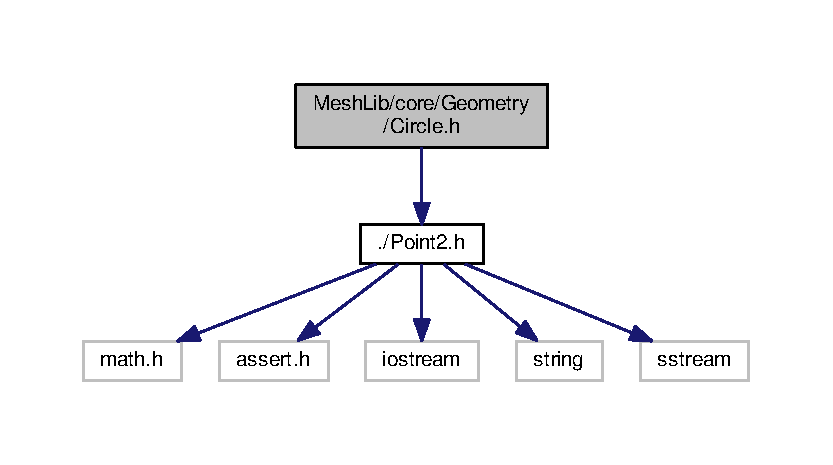
\includegraphics[width=350pt]{_circle_8h__incl}
\end{center}
\end{figure}
This graph shows which files directly or indirectly include this file\+:
\nopagebreak
\begin{figure}[H]
\begin{center}
\leavevmode
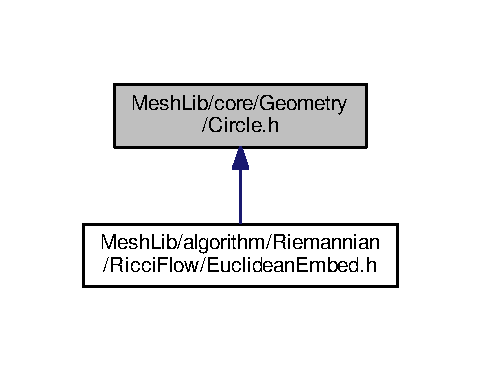
\includegraphics[width=231pt]{_circle_8h__dep__incl}
\end{center}
\end{figure}
\subsection*{Classes}
\begin{DoxyCompactItemize}
\item 
class \hyperlink{class_mesh_lib_1_1_c_circle}{Mesh\+Lib\+::\+C\+Circle}
\begin{DoxyCompactList}\small\item\em \hyperlink{class_mesh_lib_1_1_c_circle}{C\+Circle} class, circle on the plane. \end{DoxyCompactList}\end{DoxyCompactItemize}
\subsection*{Namespaces}
\begin{DoxyCompactItemize}
\item 
 \hyperlink{namespace_mesh_lib}{Mesh\+Lib}
\end{DoxyCompactItemize}
\subsection*{Functions}
\begin{DoxyCompactItemize}
\item 
C\+Circle \hyperlink{namespace_mesh_lib_ab6a6d932f384fb9578367cefca9f3b38}{Mesh\+Lib\+::orthogonal} (C\+Circle C\mbox{[}3\mbox{]})
\item 
int \hyperlink{namespace_mesh_lib_a072ef33d5d14e9cc879d55884baef73f}{Mesh\+Lib\+::\+\_\+circle\+\_\+circle\+\_\+intersection} (C\+Circle C0, C\+Circle C1, C\+Point2 \&p0, C\+Point2 \&p1)
\end{DoxyCompactItemize}


\subsection{Detailed Description}
Planar circle. 

\begin{DoxyAuthor}{Author}
David Gu 
\end{DoxyAuthor}
\begin{DoxyDate}{Date}
10/19/2010 
\end{DoxyDate}

\hypertarget{_point_8h}{}\section{Mesh\+Lib/core/\+Geometry/\+Point.h File Reference}
\label{_point_8h}\index{Mesh\+Lib/core/\+Geometry/\+Point.\+h@{Mesh\+Lib/core/\+Geometry/\+Point.\+h}}


Three dimensional point class.  


{\ttfamily \#include $<$assert.\+h$>$}\\*
{\ttfamily \#include $<$math.\+h$>$}\\*
{\ttfamily \#include $<$string$>$}\\*
{\ttfamily \#include $<$sstream$>$}\\*
Include dependency graph for Point.\+h\+:
\nopagebreak
\begin{figure}[H]
\begin{center}
\leavevmode
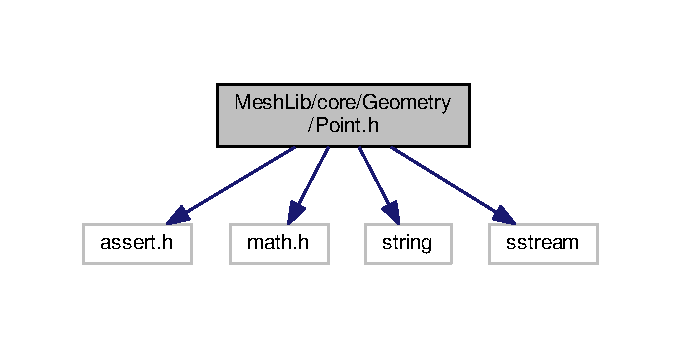
\includegraphics[width=327pt]{_point_8h__incl}
\end{center}
\end{figure}
This graph shows which files directly or indirectly include this file\+:
\nopagebreak
\begin{figure}[H]
\begin{center}
\leavevmode
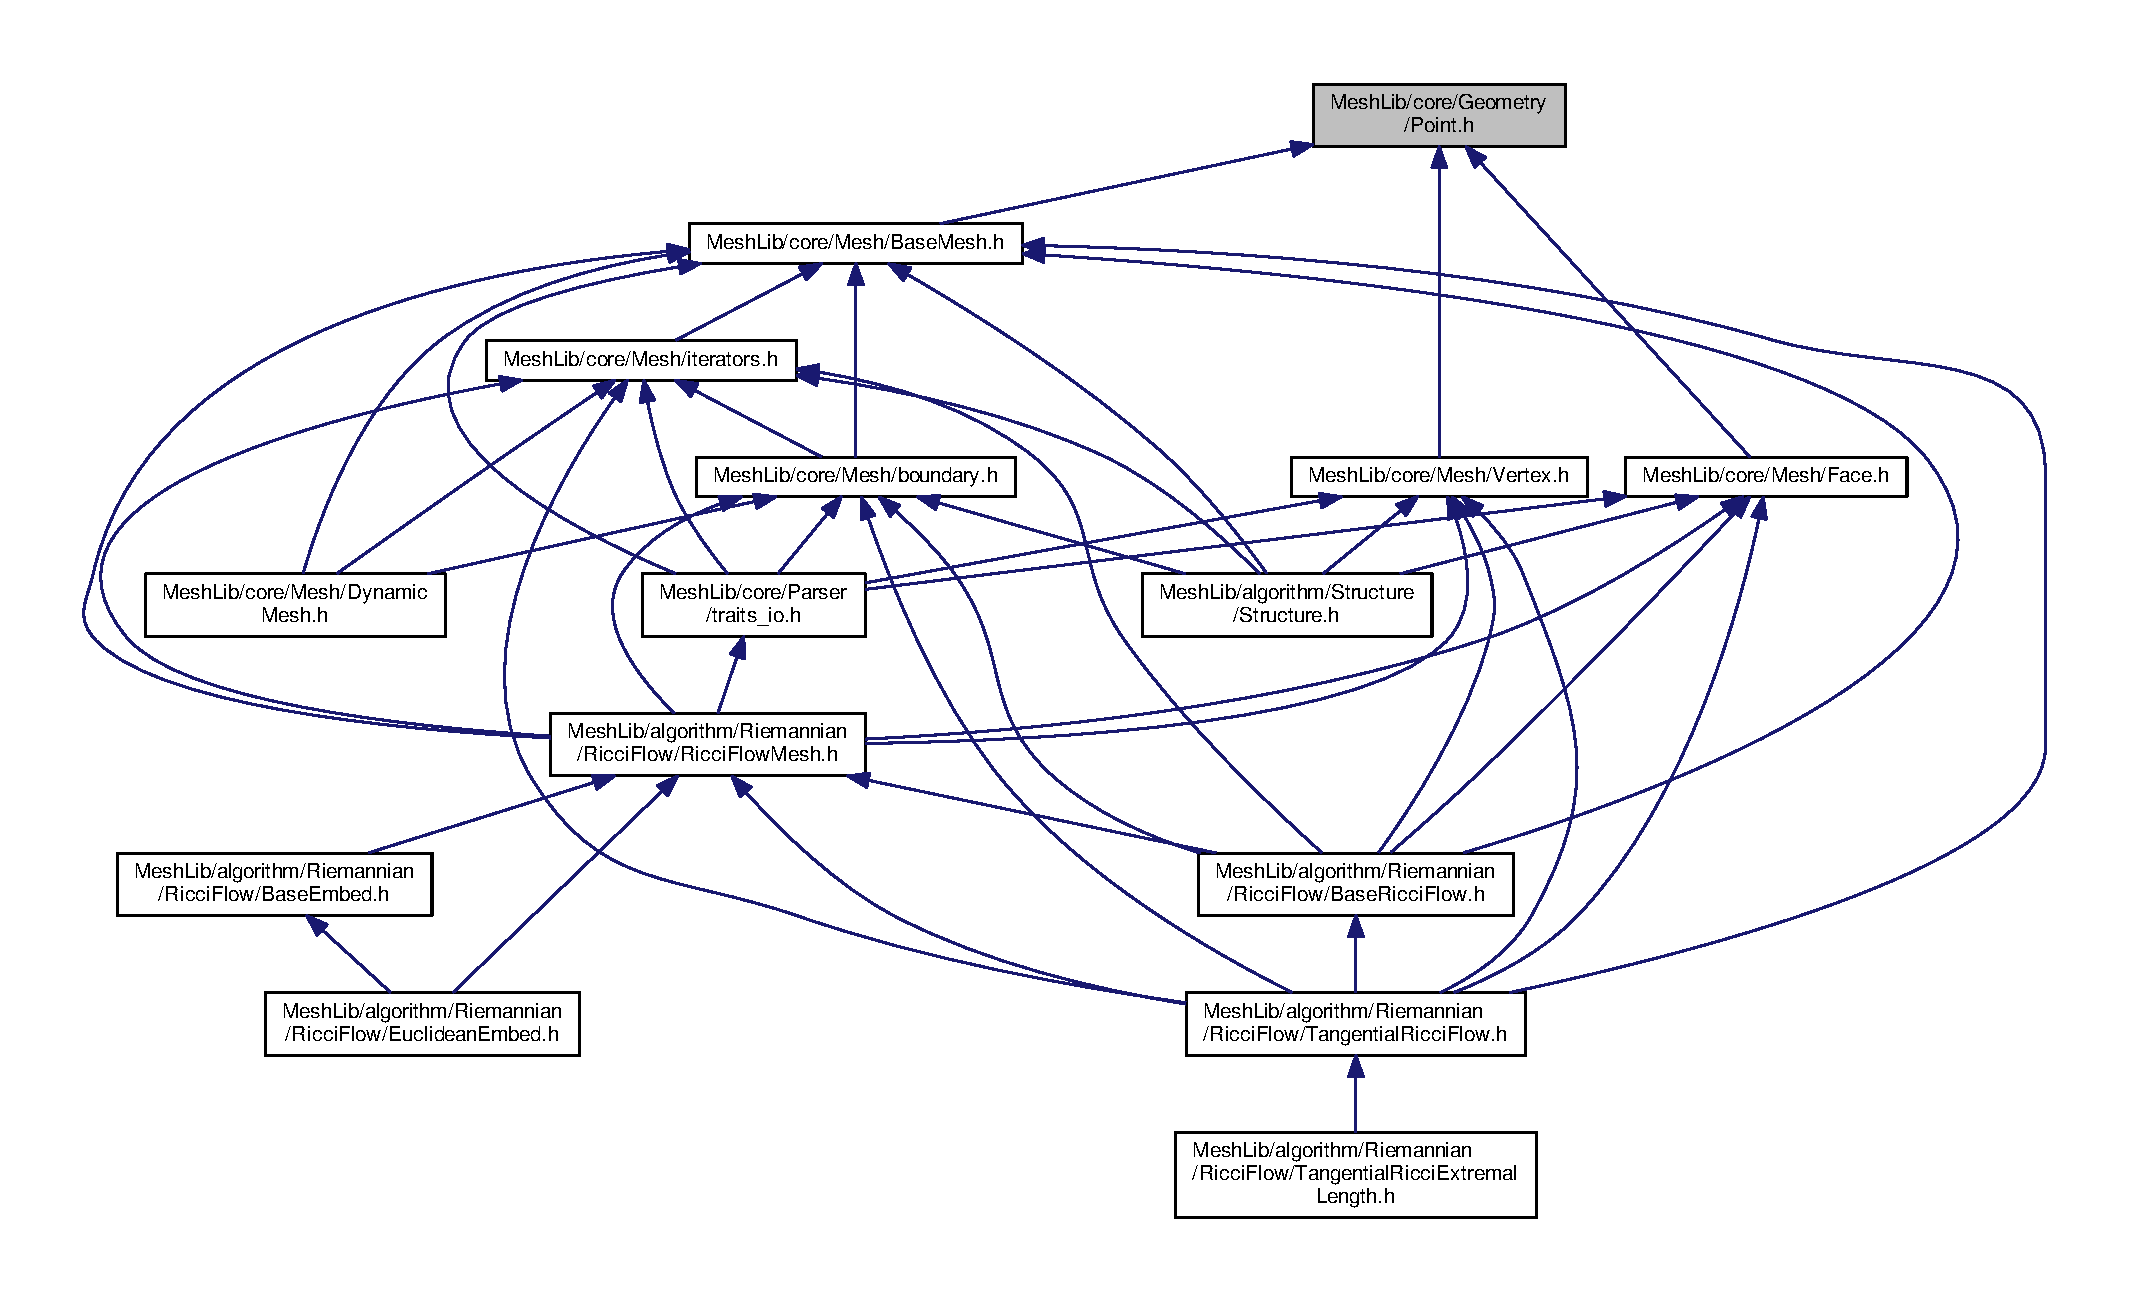
\includegraphics[width=350pt]{_point_8h__dep__incl}
\end{center}
\end{figure}
\subsection*{Classes}
\begin{DoxyCompactItemize}
\item 
class \hyperlink{class_mesh_lib_1_1_c_point}{Mesh\+Lib\+::\+C\+Point}
\begin{DoxyCompactList}\small\item\em \hyperlink{class_mesh_lib_1_1_c_point}{C\+Point} class, three dimensional point. \end{DoxyCompactList}\end{DoxyCompactItemize}
\subsection*{Namespaces}
\begin{DoxyCompactItemize}
\item 
 \hyperlink{namespace_mesh_lib}{Mesh\+Lib}
\end{DoxyCompactItemize}
\subsection*{Functions}
\begin{DoxyCompactItemize}
\item 
void \hyperlink{namespace_mesh_lib_a6697ead353dba659c806ddcfb0baf487}{Mesh\+Lib\+::operator$>$$>$} (const std\+::string \&str, C\+Point \&p)
\end{DoxyCompactItemize}


\subsection{Detailed Description}
Three dimensional point class. 

\begin{DoxyAuthor}{Author}
David Gu 
\end{DoxyAuthor}
\begin{DoxyDate}{Date}
10/07/2010 
\end{DoxyDate}

\hypertarget{_point2_8h}{}\section{Mesh\+Lib/core/\+Geometry/\+Point2.h File Reference}
\label{_point2_8h}\index{Mesh\+Lib/core/\+Geometry/\+Point2.\+h@{Mesh\+Lib/core/\+Geometry/\+Point2.\+h}}


Two dimensional point class.  


{\ttfamily \#include $<$math.\+h$>$}\\*
{\ttfamily \#include $<$assert.\+h$>$}\\*
{\ttfamily \#include $<$iostream$>$}\\*
{\ttfamily \#include $<$string$>$}\\*
{\ttfamily \#include $<$sstream$>$}\\*
Include dependency graph for Point2.\+h\+:
\nopagebreak
\begin{figure}[H]
\begin{center}
\leavevmode
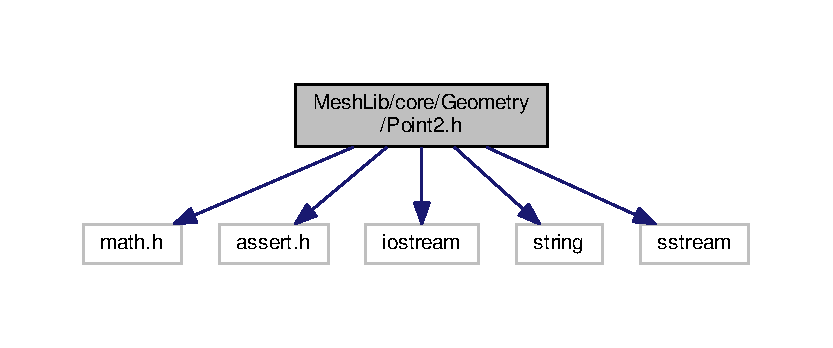
\includegraphics[width=350pt]{_point2_8h__incl}
\end{center}
\end{figure}
This graph shows which files directly or indirectly include this file\+:
\nopagebreak
\begin{figure}[H]
\begin{center}
\leavevmode
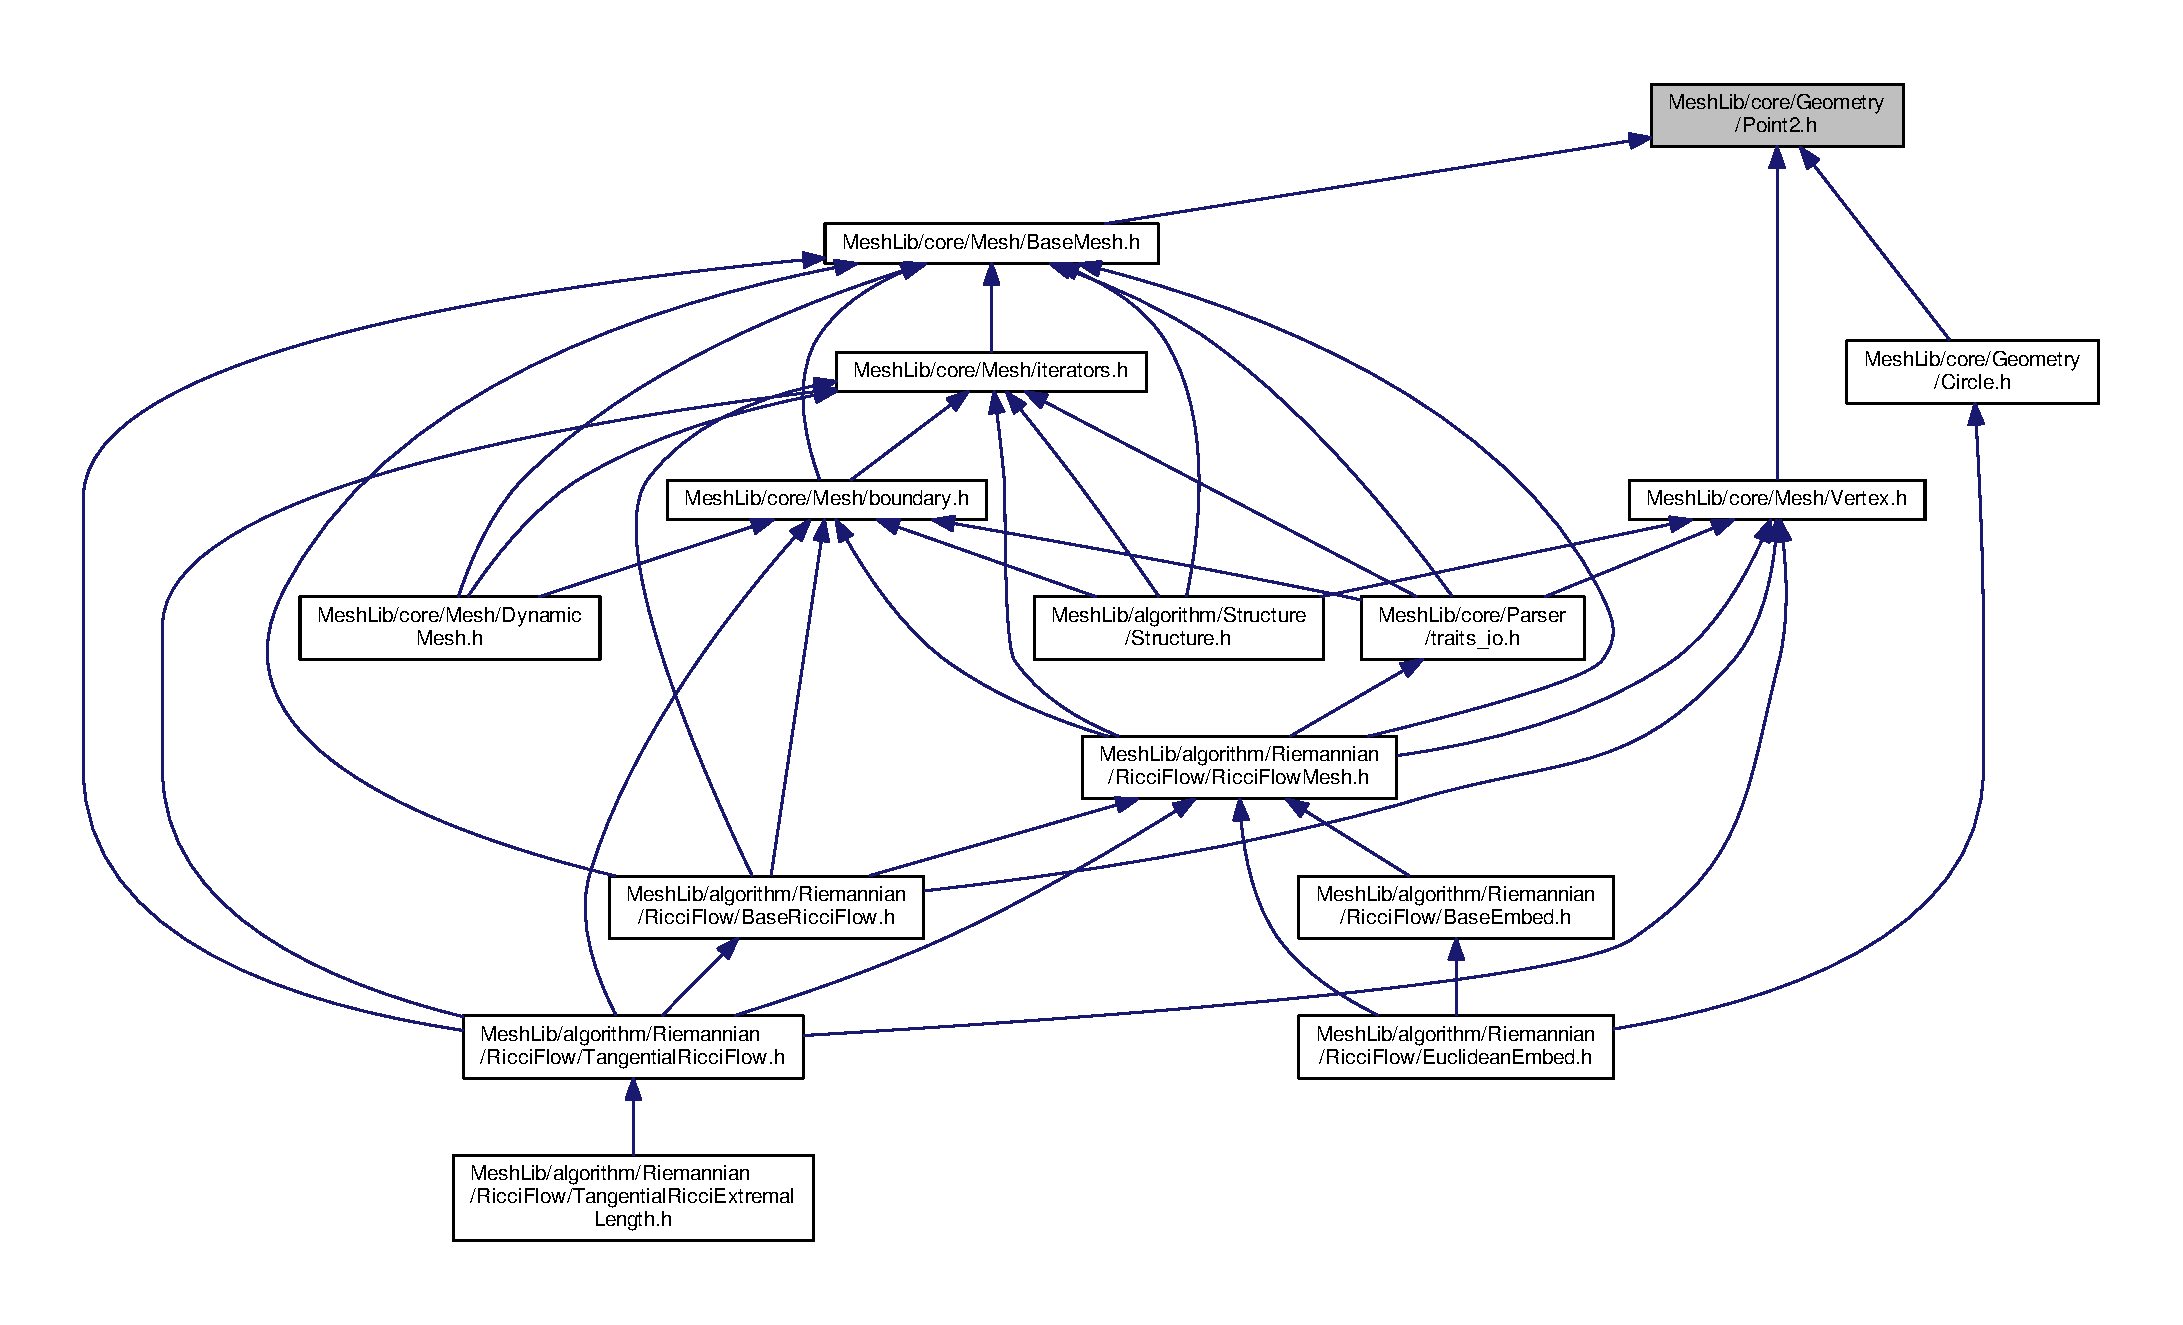
\includegraphics[width=350pt]{_point2_8h__dep__incl}
\end{center}
\end{figure}
\subsection*{Classes}
\begin{DoxyCompactItemize}
\item 
class \hyperlink{class_mesh_lib_1_1_c_point2}{Mesh\+Lib\+::\+C\+Point2}
\begin{DoxyCompactList}\small\item\em \hyperlink{class_mesh_lib_1_1_c_point2}{C\+Point2} class, two dimensional point. \end{DoxyCompactList}\end{DoxyCompactItemize}
\subsection*{Namespaces}
\begin{DoxyCompactItemize}
\item 
 \hyperlink{namespace_mesh_lib}{Mesh\+Lib}
\end{DoxyCompactItemize}
\subsection*{Functions}
\begin{DoxyCompactItemize}
\item 
C\+Point2 \hyperlink{namespace_mesh_lib_aeacba552862f8445b222e130ff81f578}{Mesh\+Lib\+::operator+} (C\+Point2 \&uv0, C\+Point2 \&uv1)
\item 
C\+Point2 \hyperlink{namespace_mesh_lib_a06843ee204e7d5adb0f8709c0388b52f}{Mesh\+Lib\+::operator-\/} (C\+Point2 \&uv0, C\+Point2 \&uv1)
\item 
C\+Point2 \hyperlink{namespace_mesh_lib_ad2193c7504c0ea252000b503b887f977}{Mesh\+Lib\+::operator$\ast$} (C\+Point2 \&uv0, const double s)
\item 
C\+Point2 \hyperlink{namespace_mesh_lib_a9938d2b3974eb39cf1ec9067f9c0c48b}{Mesh\+Lib\+::operator/} (C\+Point2 \&uv0, const double s)
\item 
C\+Point2 \hyperlink{namespace_mesh_lib_ab3f63719ad0e28580cfbb25f9af38da7}{Mesh\+Lib\+::operator+} (const C\+Point2 \&uv0, const C\+Point2 \&uv1)
\item 
C\+Point2 \hyperlink{namespace_mesh_lib_a40e50ff27b1a51bfb49fffee095133a4}{Mesh\+Lib\+::operator-\/} (const C\+Point2 \&uv0, const C\+Point2 \&uv1)
\item 
C\+Point2 \hyperlink{namespace_mesh_lib_a8d5edb06e9ddc9bcd3b978853603f9be}{Mesh\+Lib\+::operator$\ast$} (const C\+Point2 \&uv0, const double s)
\item 
C\+Point2 \hyperlink{namespace_mesh_lib_a0bb356861876e4732adba54c4b4f1816}{Mesh\+Lib\+::operator/} (const C\+Point2 \&uv0, const double s)
\item 
double \hyperlink{namespace_mesh_lib_af2c139d9c9d6112e8e72508d7e5c6bcf}{Mesh\+Lib\+::mag2} (C\+Point2 \&uv)
\item 
double \hyperlink{namespace_mesh_lib_afc6768df7d6cacb0068fd7f24038b154}{Mesh\+Lib\+::mag} (C\+Point2 \&uv)
\item 
double \hyperlink{namespace_mesh_lib_a2ade6b60ae078fba88d883854f653f84}{Mesh\+Lib\+::cross} (C\+Point2 uv1, C\+Point2 uv2)
\item 
double \hyperlink{namespace_mesh_lib_aebfbcaa5edd6ab9a3ff4cea0946932b7}{Mesh\+Lib\+::operator$\ast$} (C\+Point2 a, C\+Point2 b)
\item 
double \hyperlink{namespace_mesh_lib_ab10449a08569b7043e65ddd4b02fce35}{Mesh\+Lib\+::operator$^\wedge$} (C\+Point2 uv1, C\+Point2 uv2)
\item 
void \hyperlink{namespace_mesh_lib_a60590be9181e047574356d660f294629}{Mesh\+Lib\+::operator$>$$>$} (const std\+::string \&str, C\+Point2 \&c)
\end{DoxyCompactItemize}


\subsection{Detailed Description}
Two dimensional point class. 

\begin{DoxyAuthor}{Author}
David Gu 
\end{DoxyAuthor}
\begin{DoxyDate}{Date}
10/07/2010 
\end{DoxyDate}

\hypertarget{_base_mesh_8h}{}\section{Mesh\+Lib/core/\+Mesh/\+Base\+Mesh.h File Reference}
\label{_base_mesh_8h}\index{Mesh\+Lib/core/\+Mesh/\+Base\+Mesh.\+h@{Mesh\+Lib/core/\+Mesh/\+Base\+Mesh.\+h}}


Base Mesh Class for all types of Mesh Classes.  


{\ttfamily \#include $<$math.\+h$>$}\\*
{\ttfamily \#include $<$assert.\+h$>$}\\*
{\ttfamily \#include $<$iostream$>$}\\*
{\ttfamily \#include $<$fstream$>$}\\*
{\ttfamily \#include $<$list$>$}\\*
{\ttfamily \#include $<$vector$>$}\\*
{\ttfamily \#include $<$map$>$}\\*
{\ttfamily \#include \char`\"{}../\+Geometry/\+Point.\+h\char`\"{}}\\*
{\ttfamily \#include \char`\"{}../\+Geometry/\+Point2.\+h\char`\"{}}\\*
{\ttfamily \#include \char`\"{}../\+Parser/strutil.\+h\char`\"{}}\\*
Include dependency graph for Base\+Mesh.\+h\+:
\nopagebreak
\begin{figure}[H]
\begin{center}
\leavevmode
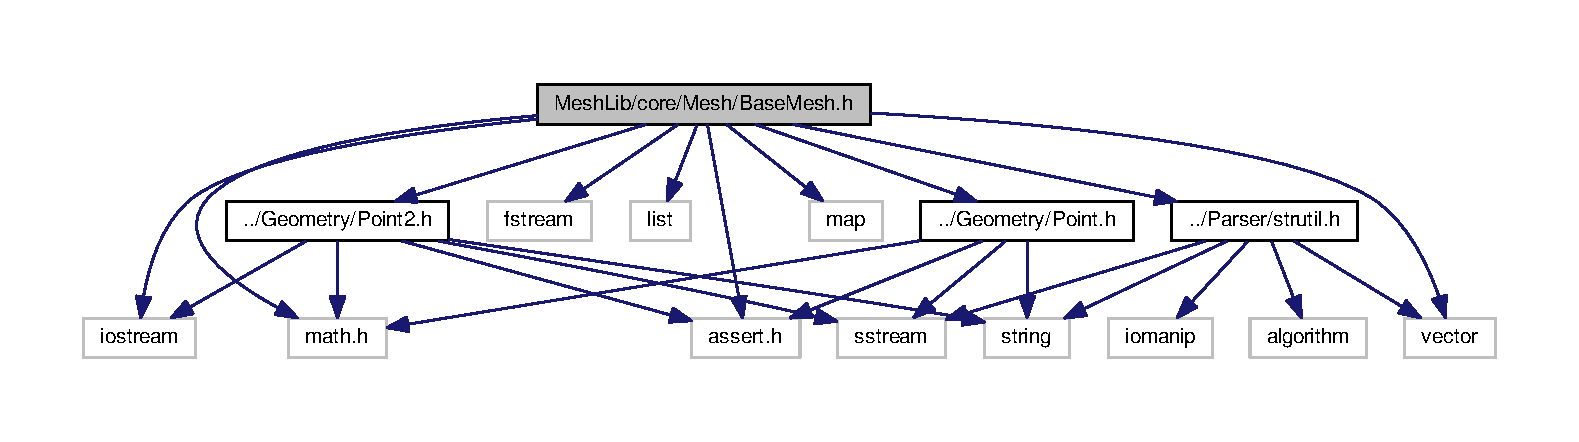
\includegraphics[width=350pt]{_base_mesh_8h__incl}
\end{center}
\end{figure}
This graph shows which files directly or indirectly include this file\+:
\nopagebreak
\begin{figure}[H]
\begin{center}
\leavevmode
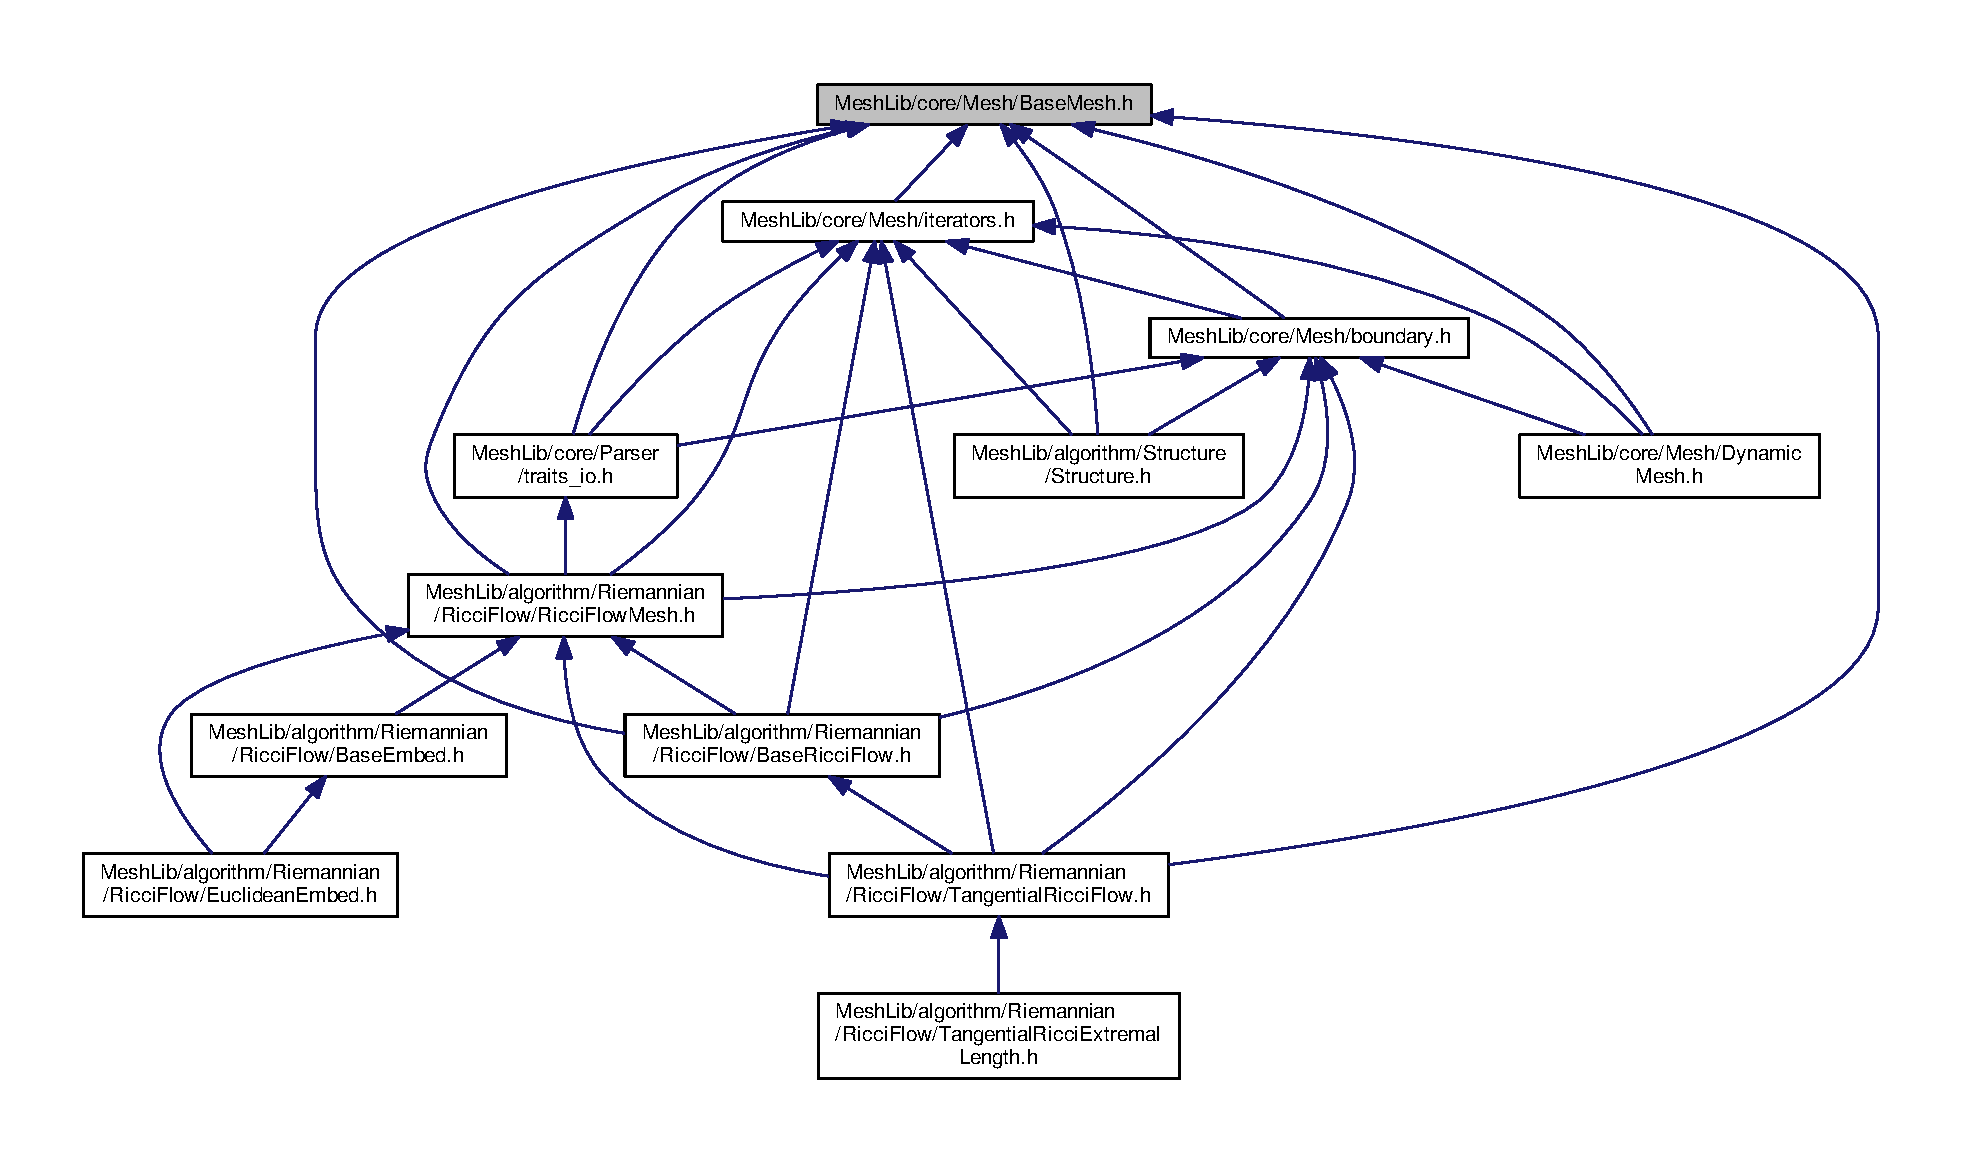
\includegraphics[width=350pt]{_base_mesh_8h__dep__incl}
\end{center}
\end{figure}
\subsection*{Classes}
\begin{DoxyCompactItemize}
\item 
class \hyperlink{class_mesh_lib_1_1_c_base_mesh}{Mesh\+Lib\+::\+C\+Base\+Mesh$<$ C\+Vertex, C\+Edge, C\+Face, C\+Half\+Edge $>$}
\begin{DoxyCompactList}\small\item\em \hyperlink{class_mesh_lib_1_1_c_base_mesh}{C\+Base\+Mesh}, base class for all types of mesh classes. \end{DoxyCompactList}\end{DoxyCompactItemize}
\subsection*{Namespaces}
\begin{DoxyCompactItemize}
\item 
 \hyperlink{namespace_mesh_lib}{Mesh\+Lib}
\end{DoxyCompactItemize}
\subsection*{Macros}
\begin{DoxyCompactItemize}
\item 
\#define \hyperlink{_base_mesh_8h_a842ed03f27719bc87666bfd1f75415b8}{M\+A\+X\+\_\+\+L\+I\+NE}~2048
\end{DoxyCompactItemize}


\subsection{Detailed Description}
Base Mesh Class for all types of Mesh Classes. 

This is the fundamental class for meshes \begin{DoxyAuthor}{Author}
David Gu 
\end{DoxyAuthor}
\begin{DoxyDate}{Date}
10/07/2010 
\end{DoxyDate}


\subsection{Macro Definition Documentation}
\index{Base\+Mesh.\+h@{Base\+Mesh.\+h}!M\+A\+X\+\_\+\+L\+I\+NE@{M\+A\+X\+\_\+\+L\+I\+NE}}
\index{M\+A\+X\+\_\+\+L\+I\+NE@{M\+A\+X\+\_\+\+L\+I\+NE}!Base\+Mesh.\+h@{Base\+Mesh.\+h}}
\subsubsection[{\texorpdfstring{M\+A\+X\+\_\+\+L\+I\+NE}{MAX_LINE}}]{\setlength{\rightskip}{0pt plus 5cm}\#define M\+A\+X\+\_\+\+L\+I\+NE~2048}\hypertarget{_base_mesh_8h_a842ed03f27719bc87666bfd1f75415b8}{}\label{_base_mesh_8h_a842ed03f27719bc87666bfd1f75415b8}


Definition at line 14 of file Base\+Mesh.\+h.


\hypertarget{boundary_8h}{}\section{Mesh\+Lib/core/\+Mesh/boundary.h File Reference}
\label{boundary_8h}\index{Mesh\+Lib/core/\+Mesh/boundary.\+h@{Mesh\+Lib/core/\+Mesh/boundary.\+h}}
{\ttfamily \#include $<$iostream$>$}\\*
{\ttfamily \#include $<$fstream$>$}\\*
{\ttfamily \#include $<$algorithm$>$}\\*
{\ttfamily \#include $<$vector$>$}\\*
{\ttfamily \#include $<$list$>$}\\*
{\ttfamily \#include $<$set$>$}\\*
{\ttfamily \#include \char`\"{}./\+Base\+Mesh.\+h\char`\"{}}\\*
{\ttfamily \#include \char`\"{}./iterators.\+h\char`\"{}}\\*
Include dependency graph for boundary.\+h\+:
\nopagebreak
\begin{figure}[H]
\begin{center}
\leavevmode
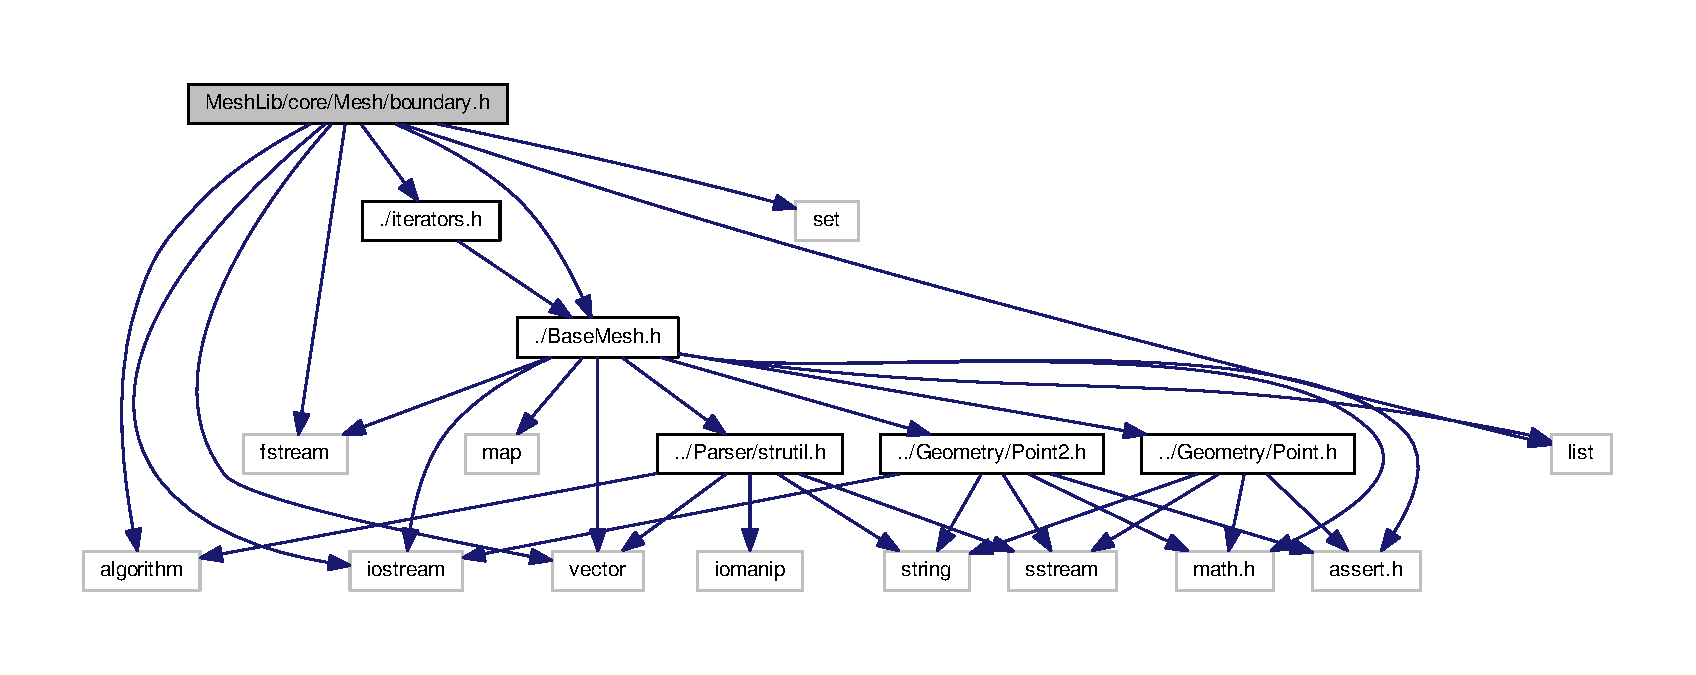
\includegraphics[width=350pt]{boundary_8h__incl}
\end{center}
\end{figure}
This graph shows which files directly or indirectly include this file\+:
\nopagebreak
\begin{figure}[H]
\begin{center}
\leavevmode
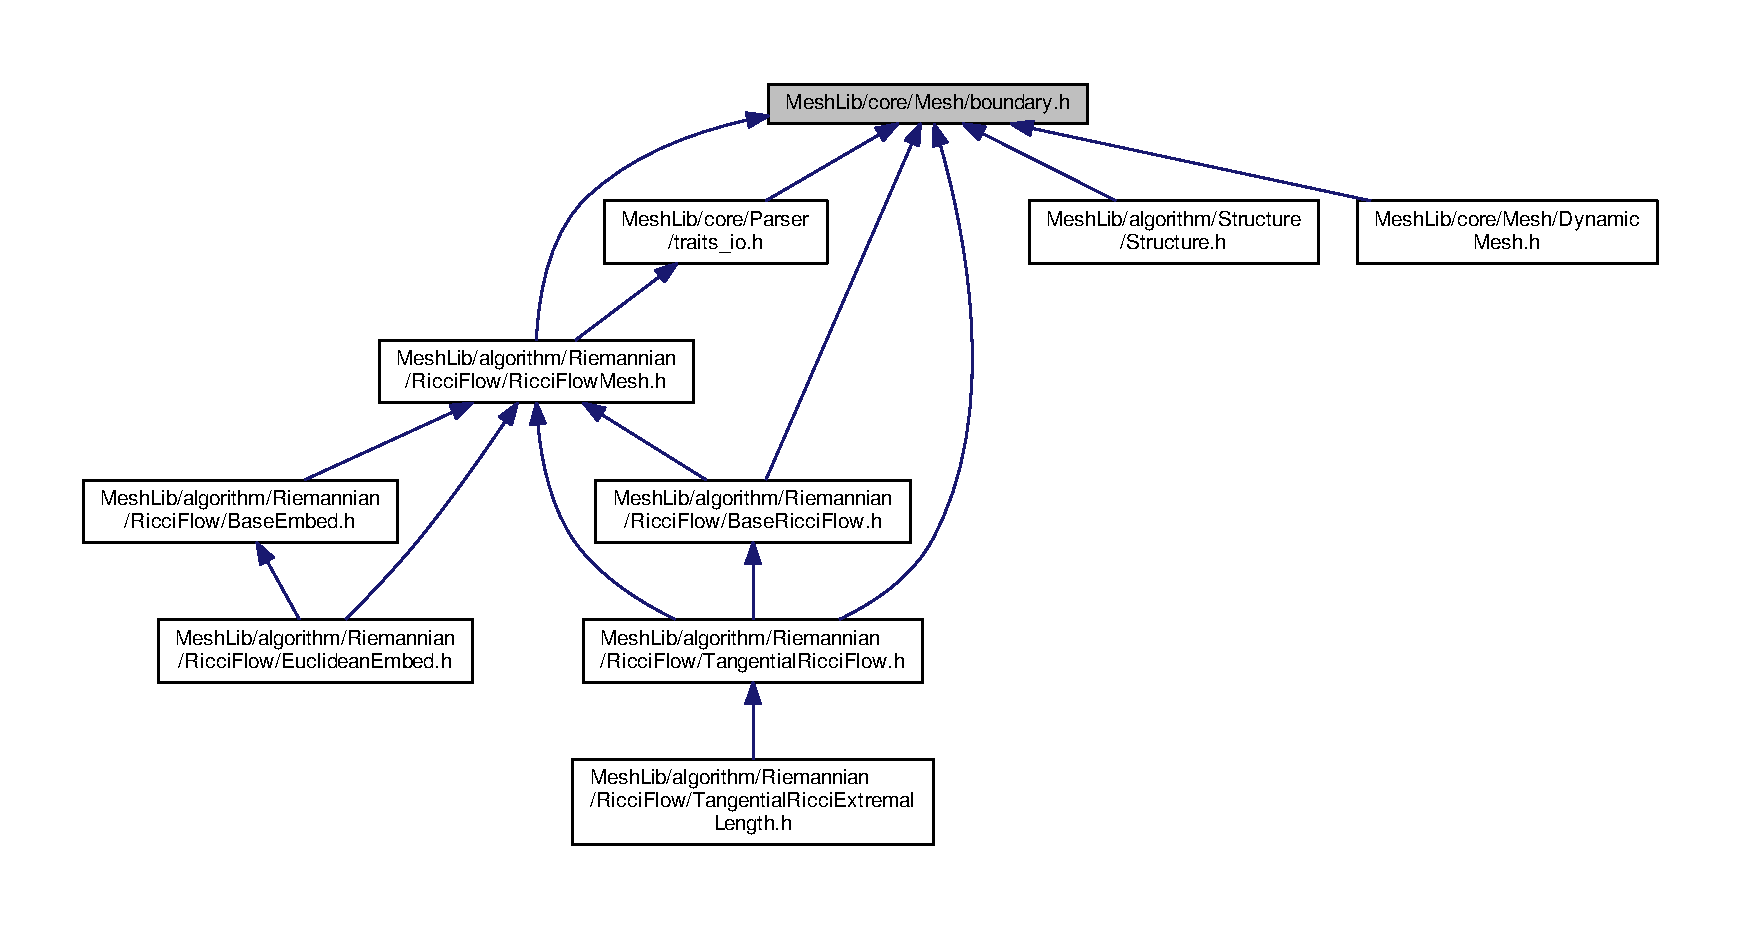
\includegraphics[width=350pt]{boundary_8h__dep__incl}
\end{center}
\end{figure}
\subsection*{Classes}
\begin{DoxyCompactItemize}
\item 
class \hyperlink{class_mesh_lib_1_1_c_loop}{Mesh\+Lib\+::\+C\+Loop$<$ C\+Vertex, C\+Edge, C\+Face, C\+Half\+Edge $>$}
\begin{DoxyCompactList}\small\item\em \hyperlink{class_mesh_lib_1_1_c_loop}{C\+Loop} Boundary loop class. \end{DoxyCompactList}\item 
class \hyperlink{class_mesh_lib_1_1_c_boundary}{Mesh\+Lib\+::\+C\+Boundary$<$ C\+Vertex, C\+Edge, C\+Face, C\+Half\+Edge $>$}
\begin{DoxyCompactList}\small\item\em \hyperlink{class_mesh_lib_1_1_c_boundary}{C\+Boundary} Boundary class. \end{DoxyCompactList}\end{DoxyCompactItemize}
\subsection*{Namespaces}
\begin{DoxyCompactItemize}
\item 
 \hyperlink{namespace_mesh_lib}{Mesh\+Lib}
\end{DoxyCompactItemize}

\hypertarget{_dynamic_mesh_8h}{}\section{Mesh\+Lib/core/\+Mesh/\+Dynamic\+Mesh.h File Reference}
\label{_dynamic_mesh_8h}\index{Mesh\+Lib/core/\+Mesh/\+Dynamic\+Mesh.\+h@{Mesh\+Lib/core/\+Mesh/\+Dynamic\+Mesh.\+h}}


Dynamic Mesh Class for edge swap, face split, edge split.  


{\ttfamily \#include $<$map$>$}\\*
{\ttfamily \#include $<$vector$>$}\\*
{\ttfamily \#include $<$queue$>$}\\*
{\ttfamily \#include \char`\"{}./\+Base\+Mesh.\+h\char`\"{}}\\*
{\ttfamily \#include \char`\"{}./boundary.\+h\char`\"{}}\\*
{\ttfamily \#include \char`\"{}./iterators.\+h\char`\"{}}\\*
Include dependency graph for Dynamic\+Mesh.\+h\+:
\nopagebreak
\begin{figure}[H]
\begin{center}
\leavevmode
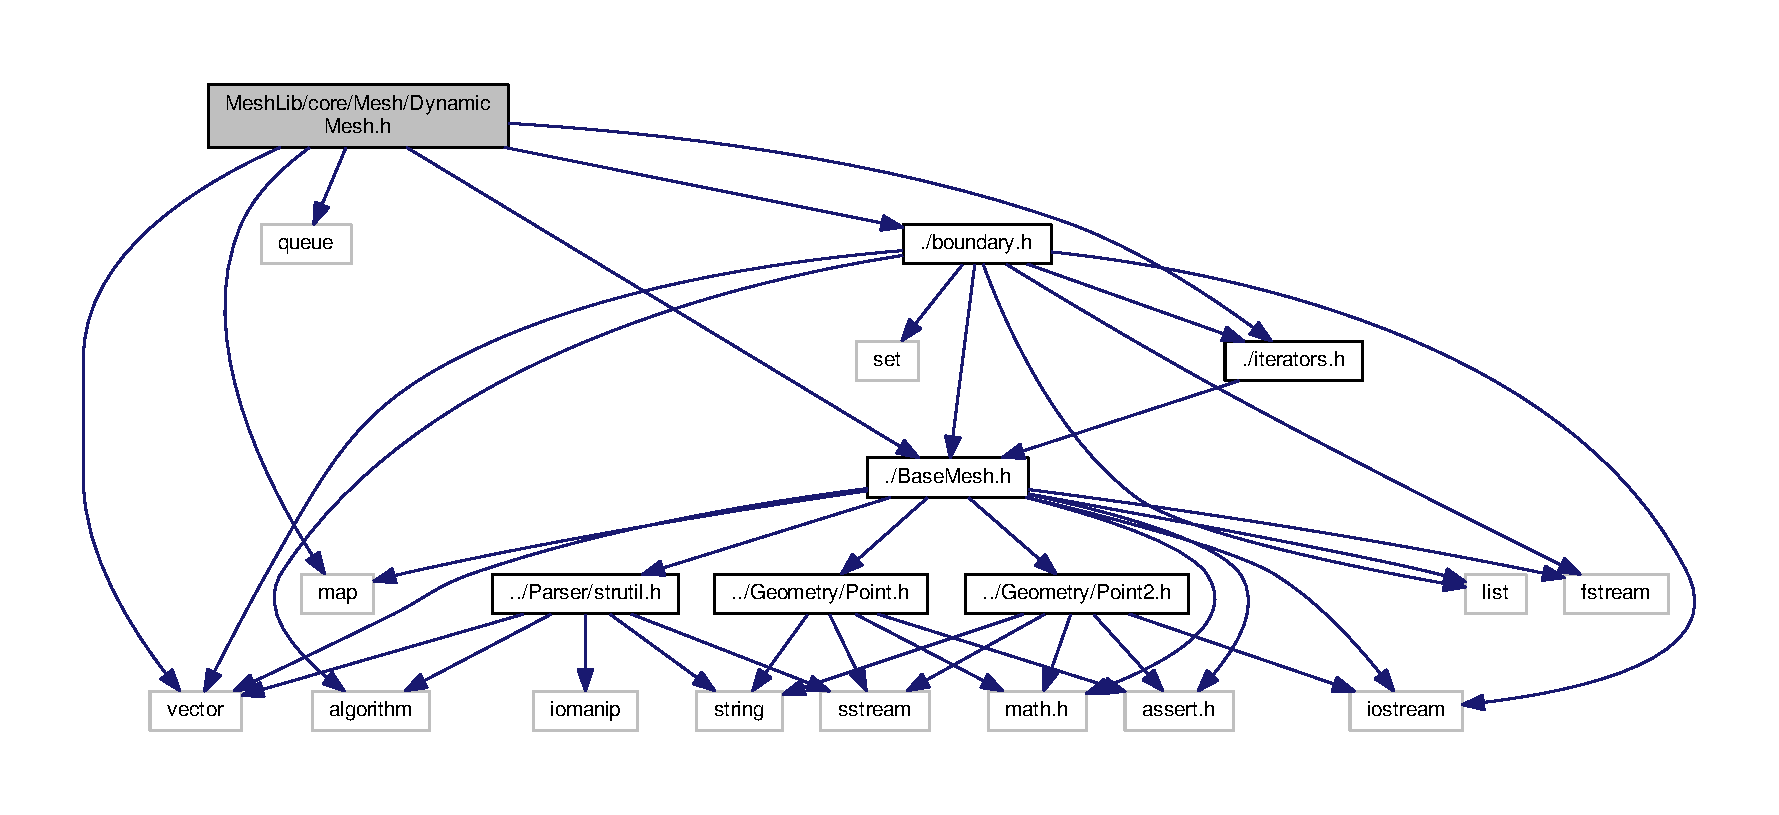
\includegraphics[width=350pt]{_dynamic_mesh_8h__incl}
\end{center}
\end{figure}
\subsection*{Classes}
\begin{DoxyCompactItemize}
\item 
class \hyperlink{class_mesh_lib_1_1_c_dynamic_mesh}{Mesh\+Lib\+::\+C\+Dynamic\+Mesh$<$ V, E, F, H $>$}
\begin{DoxyCompactList}\small\item\em \hyperlink{class_mesh_lib_1_1_c_dynamic_mesh}{C\+Dynamic\+Mesh} class \+: Dynamic mesh. \end{DoxyCompactList}\end{DoxyCompactItemize}
\subsection*{Namespaces}
\begin{DoxyCompactItemize}
\item 
 \hyperlink{namespace_mesh_lib}{Mesh\+Lib}
\end{DoxyCompactItemize}


\subsection{Detailed Description}
Dynamic Mesh Class for edge swap, face split, edge split. 

Dynamic Mesh Class for edge swap, face split, edge split \begin{DoxyAuthor}{Author}
David Gu 
\end{DoxyAuthor}
\begin{DoxyDate}{Date}
10/07/2010 
\end{DoxyDate}

\hypertarget{_edge_8h}{}\section{Mesh\+Lib/core/\+Mesh/\+Edge.h File Reference}
\label{_edge_8h}\index{Mesh\+Lib/core/\+Mesh/\+Edge.\+h@{Mesh\+Lib/core/\+Mesh/\+Edge.\+h}}


Base class of edge.  


{\ttfamily \#include $<$assert.\+h$>$}\\*
{\ttfamily \#include $<$stdlib.\+h$>$}\\*
{\ttfamily \#include $<$math.\+h$>$}\\*
{\ttfamily \#include $<$string$>$}\\*
Include dependency graph for Edge.\+h\+:
\nopagebreak
\begin{figure}[H]
\begin{center}
\leavevmode
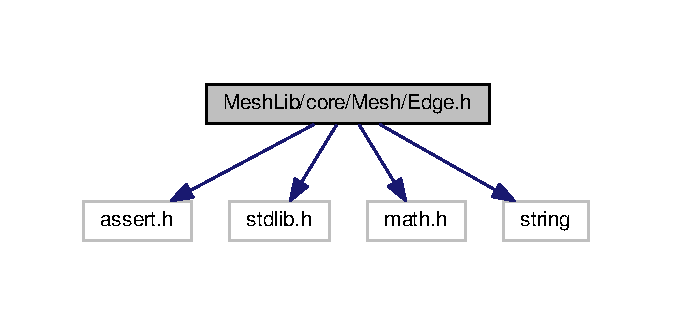
\includegraphics[width=323pt]{_edge_8h__incl}
\end{center}
\end{figure}
This graph shows which files directly or indirectly include this file\+:
\nopagebreak
\begin{figure}[H]
\begin{center}
\leavevmode
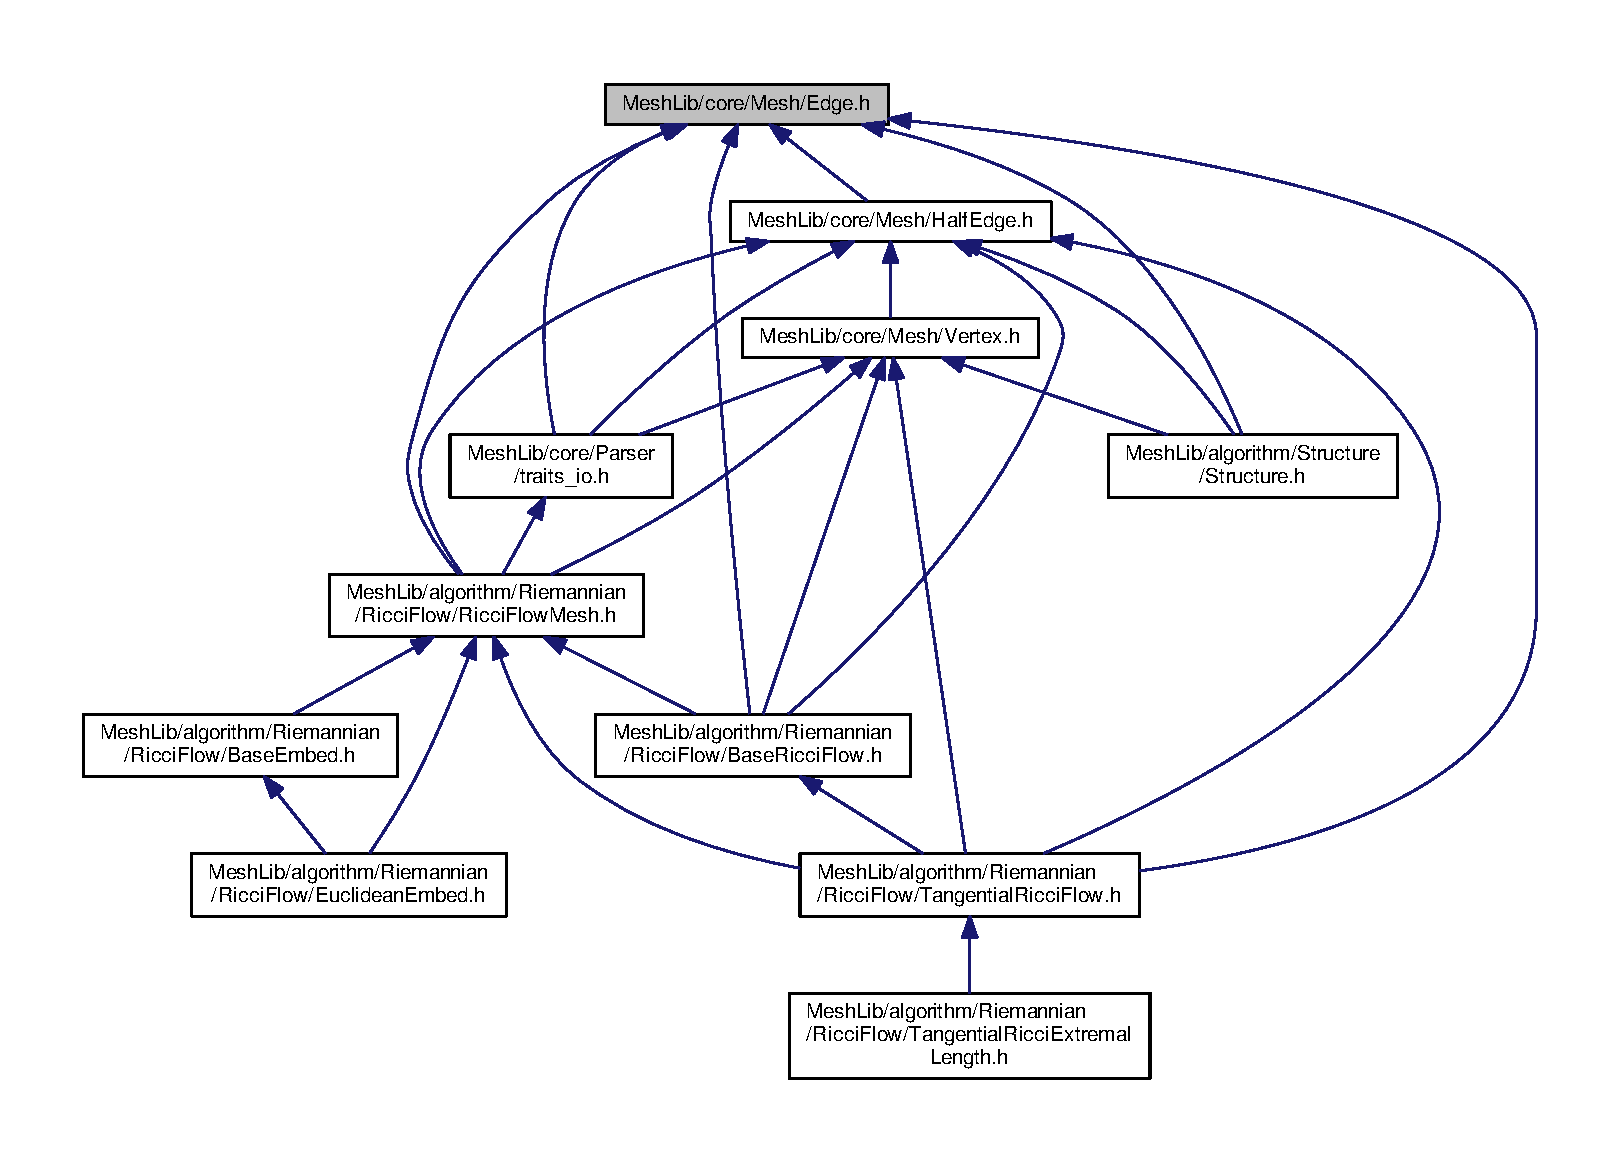
\includegraphics[width=350pt]{_edge_8h__dep__incl}
\end{center}
\end{figure}
\subsection*{Classes}
\begin{DoxyCompactItemize}
\item 
class \hyperlink{class_mesh_lib_1_1_c_edge}{Mesh\+Lib\+::\+C\+Edge}
\begin{DoxyCompactList}\small\item\em \hyperlink{class_mesh_lib_1_1_c_edge}{C\+Edge} class, which is the base class of all kinds of edge classes. \end{DoxyCompactList}\end{DoxyCompactItemize}
\subsection*{Namespaces}
\begin{DoxyCompactItemize}
\item 
 \hyperlink{namespace_mesh_lib}{Mesh\+Lib}
\end{DoxyCompactItemize}


\subsection{Detailed Description}
Base class of edge. 

\begin{DoxyAuthor}{Author}
David Gu 
\end{DoxyAuthor}
\begin{DoxyDate}{Date}
10/07/2010 
\end{DoxyDate}

\hypertarget{_face_8h}{}\section{Mesh\+Lib/core/\+Mesh/\+Face.h File Reference}
\label{_face_8h}\index{Mesh\+Lib/core/\+Mesh/\+Face.\+h@{Mesh\+Lib/core/\+Mesh/\+Face.\+h}}


Base class of face.  


{\ttfamily \#include $<$assert.\+h$>$}\\*
{\ttfamily \#include $<$string$>$}\\*
{\ttfamily \#include \char`\"{}../\+Geometry/\+Point.\+h\char`\"{}}\\*
Include dependency graph for Face.\+h\+:
\nopagebreak
\begin{figure}[H]
\begin{center}
\leavevmode
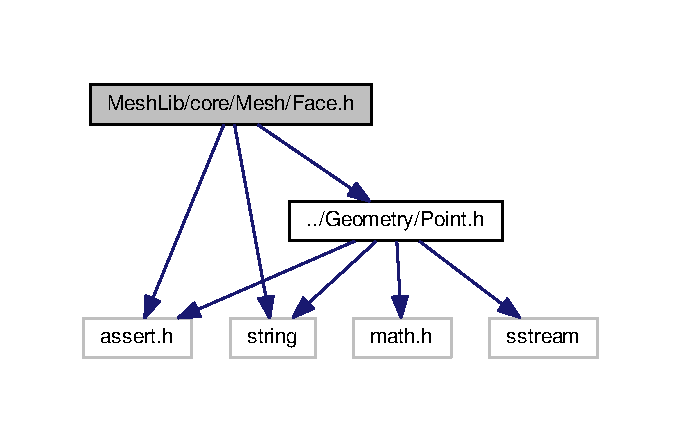
\includegraphics[width=327pt]{_face_8h__incl}
\end{center}
\end{figure}
This graph shows which files directly or indirectly include this file\+:
\nopagebreak
\begin{figure}[H]
\begin{center}
\leavevmode
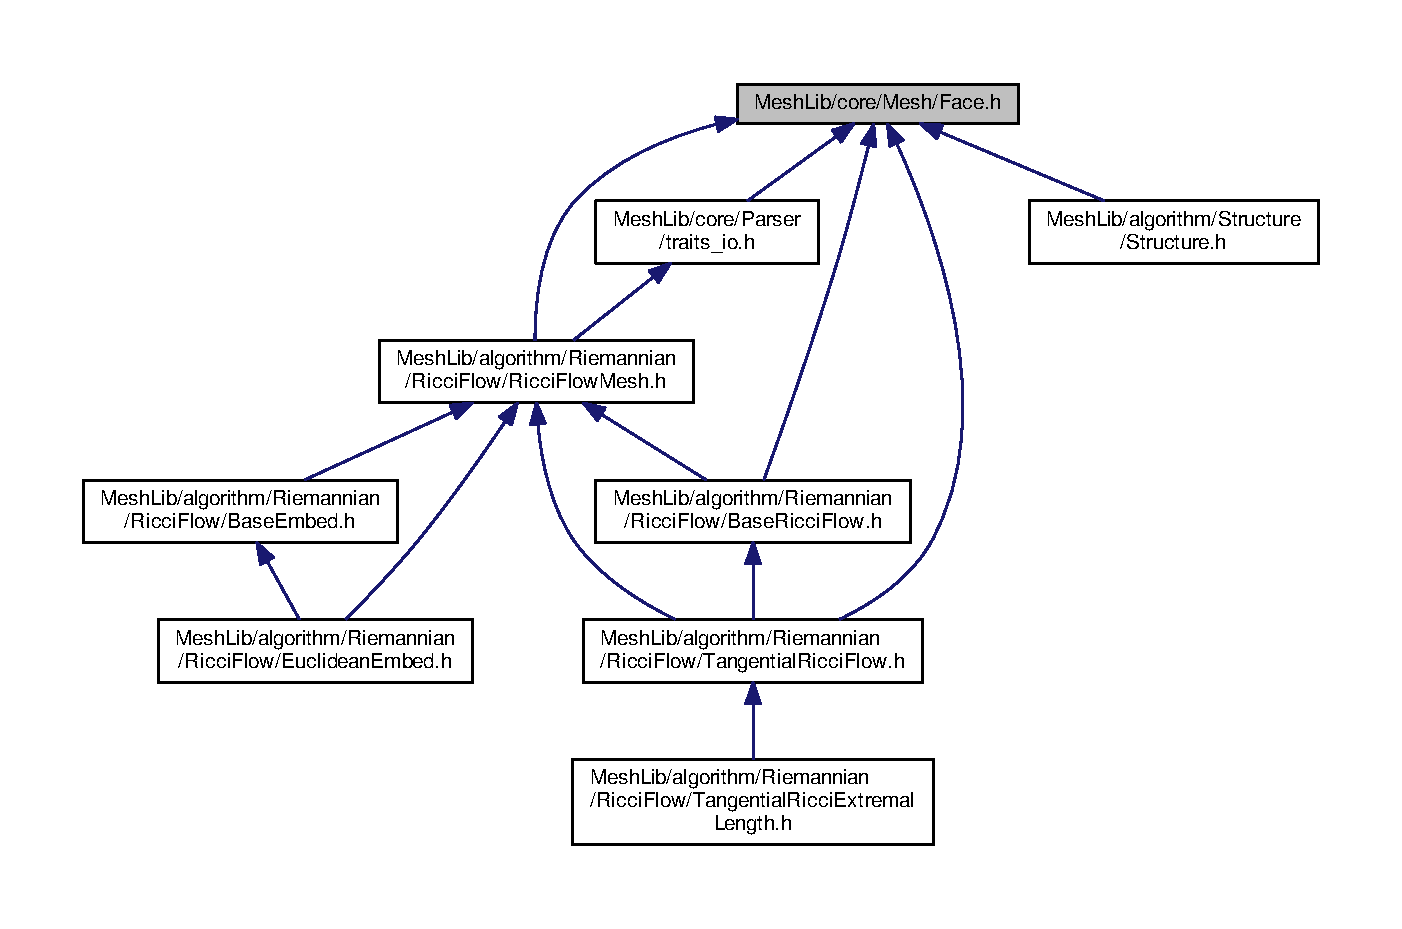
\includegraphics[width=350pt]{_face_8h__dep__incl}
\end{center}
\end{figure}
\subsection*{Classes}
\begin{DoxyCompactItemize}
\item 
class \hyperlink{class_mesh_lib_1_1_c_face}{Mesh\+Lib\+::\+C\+Face}
\begin{DoxyCompactList}\small\item\em \hyperlink{class_mesh_lib_1_1_c_face}{C\+Face} base class of all kinds of face classes. \end{DoxyCompactList}\end{DoxyCompactItemize}
\subsection*{Namespaces}
\begin{DoxyCompactItemize}
\item 
 \hyperlink{namespace_mesh_lib}{Mesh\+Lib}
\end{DoxyCompactItemize}


\subsection{Detailed Description}
Base class of face. 

\begin{DoxyAuthor}{Author}
David Gu 
\end{DoxyAuthor}
\begin{DoxyDate}{Date}
10/07/2010 
\end{DoxyDate}

\hypertarget{_half_edge_8h}{}\section{Mesh\+Lib/core/\+Mesh/\+Half\+Edge.h File Reference}
\label{_half_edge_8h}\index{Mesh\+Lib/core/\+Mesh/\+Half\+Edge.\+h@{Mesh\+Lib/core/\+Mesh/\+Half\+Edge.\+h}}


Base class of Half\+Edge.  


{\ttfamily \#include $<$assert.\+h$>$}\\*
{\ttfamily \#include $<$math.\+h$>$}\\*
{\ttfamily \#include $<$string$>$}\\*
{\ttfamily \#include \char`\"{}./\+Edge.\+h\char`\"{}}\\*
Include dependency graph for Half\+Edge.\+h\+:
\nopagebreak
\begin{figure}[H]
\begin{center}
\leavevmode
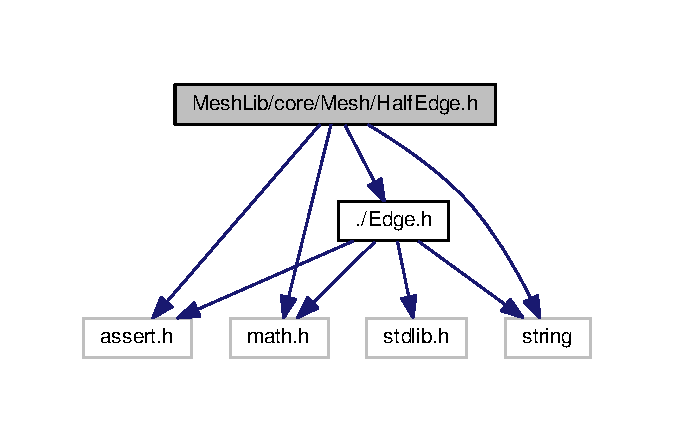
\includegraphics[width=324pt]{_half_edge_8h__incl}
\end{center}
\end{figure}
This graph shows which files directly or indirectly include this file\+:
\nopagebreak
\begin{figure}[H]
\begin{center}
\leavevmode
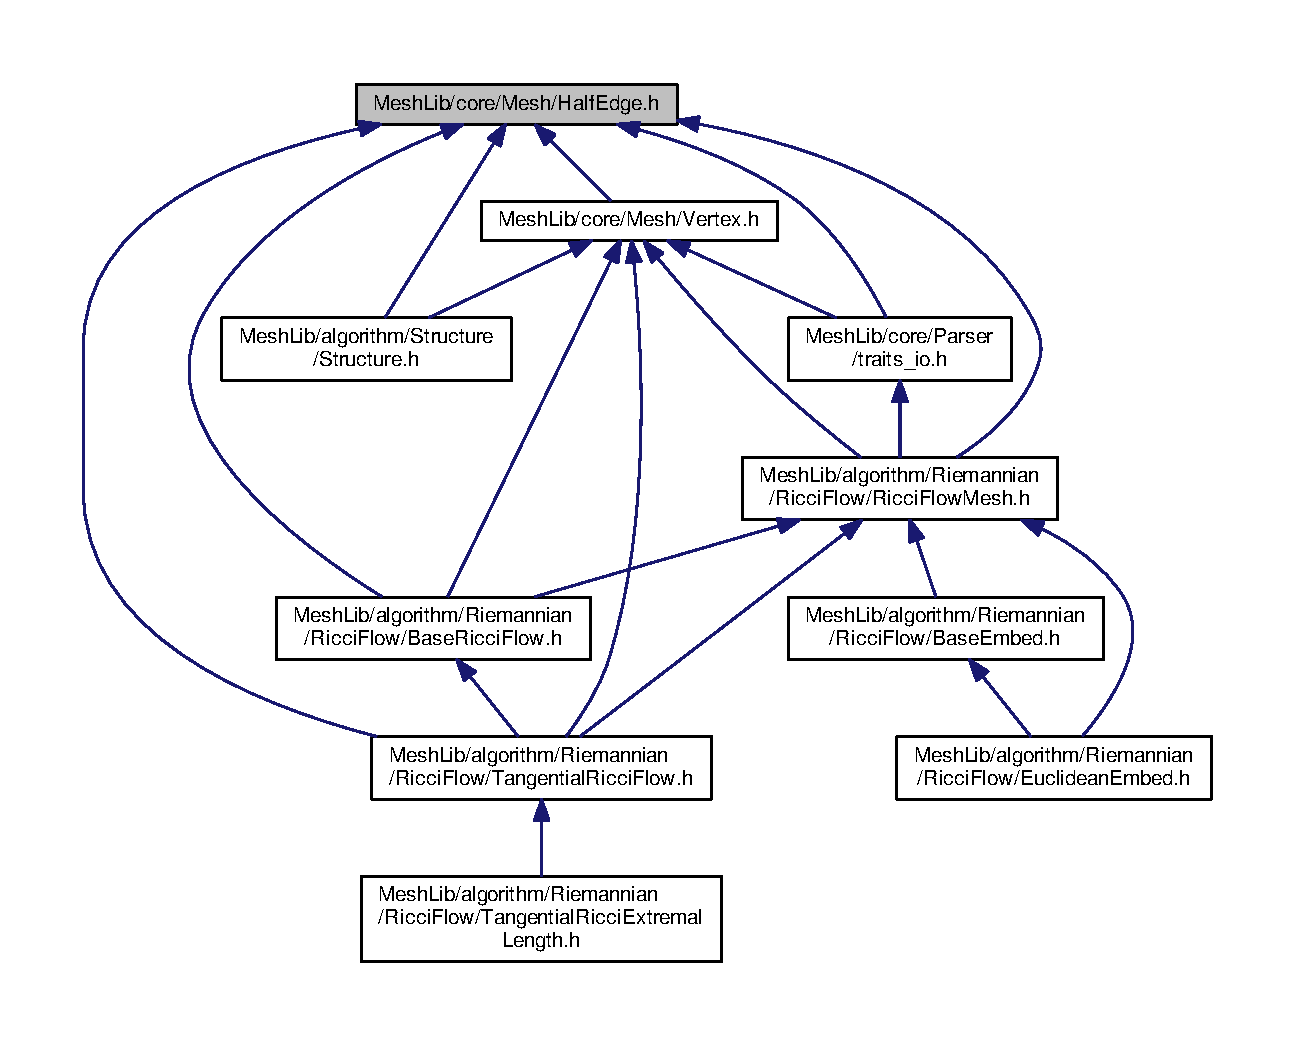
\includegraphics[width=350pt]{_half_edge_8h__dep__incl}
\end{center}
\end{figure}
\subsection*{Classes}
\begin{DoxyCompactItemize}
\item 
class \hyperlink{class_mesh_lib_1_1_c_half_edge}{Mesh\+Lib\+::\+C\+Half\+Edge}
\begin{DoxyCompactList}\small\item\em \hyperlink{class_mesh_lib_1_1_c_half_edge}{C\+Half\+Edge} Base class of all kinds of halfedges. \end{DoxyCompactList}\end{DoxyCompactItemize}
\subsection*{Namespaces}
\begin{DoxyCompactItemize}
\item 
 \hyperlink{namespace_mesh_lib}{Mesh\+Lib}
\end{DoxyCompactItemize}


\subsection{Detailed Description}
Base class of Half\+Edge. 

\begin{DoxyAuthor}{Author}
David Gu 
\end{DoxyAuthor}
\begin{DoxyDate}{Date}
10/07/2010 
\end{DoxyDate}

\hypertarget{iterators_8h}{}\section{Mesh\+Lib/core/\+Mesh/iterators.h File Reference}
\label{iterators_8h}\index{Mesh\+Lib/core/\+Mesh/iterators.\+h@{Mesh\+Lib/core/\+Mesh/iterators.\+h}}
{\ttfamily \#include \char`\"{}./\+Base\+Mesh.\+h\char`\"{}}\\*
Include dependency graph for iterators.\+h\+:
\nopagebreak
\begin{figure}[H]
\begin{center}
\leavevmode
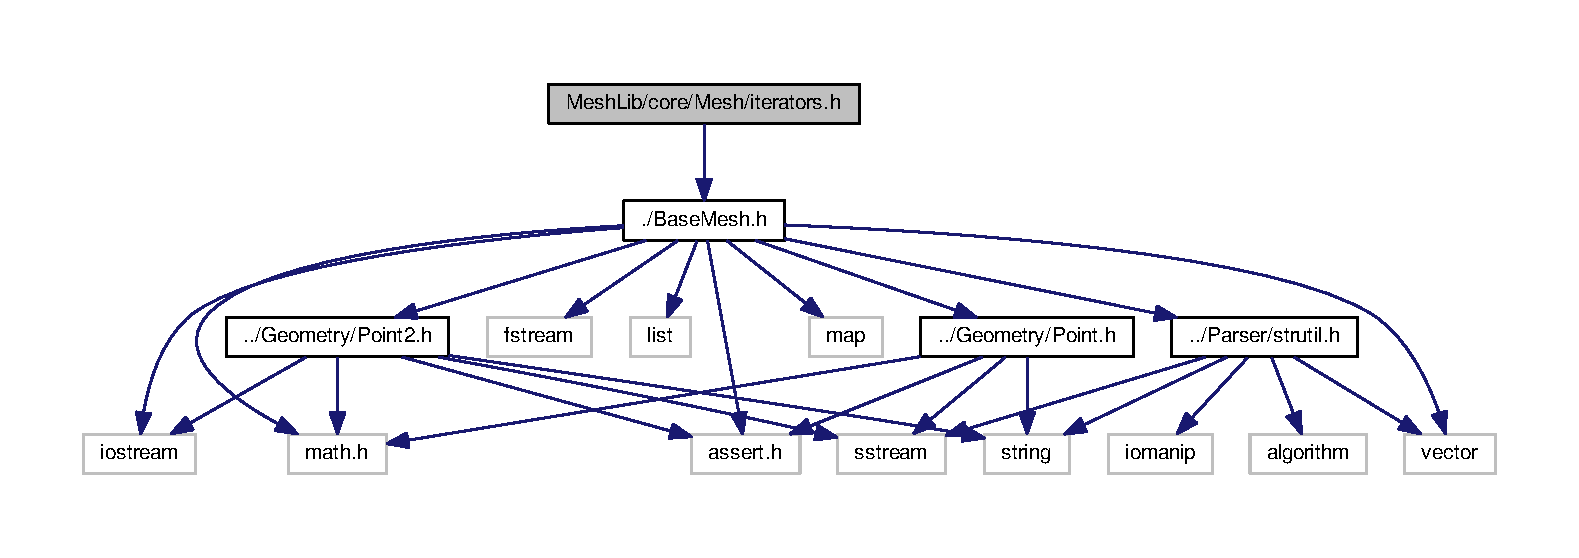
\includegraphics[width=350pt]{iterators_8h__incl}
\end{center}
\end{figure}
This graph shows which files directly or indirectly include this file\+:
\nopagebreak
\begin{figure}[H]
\begin{center}
\leavevmode
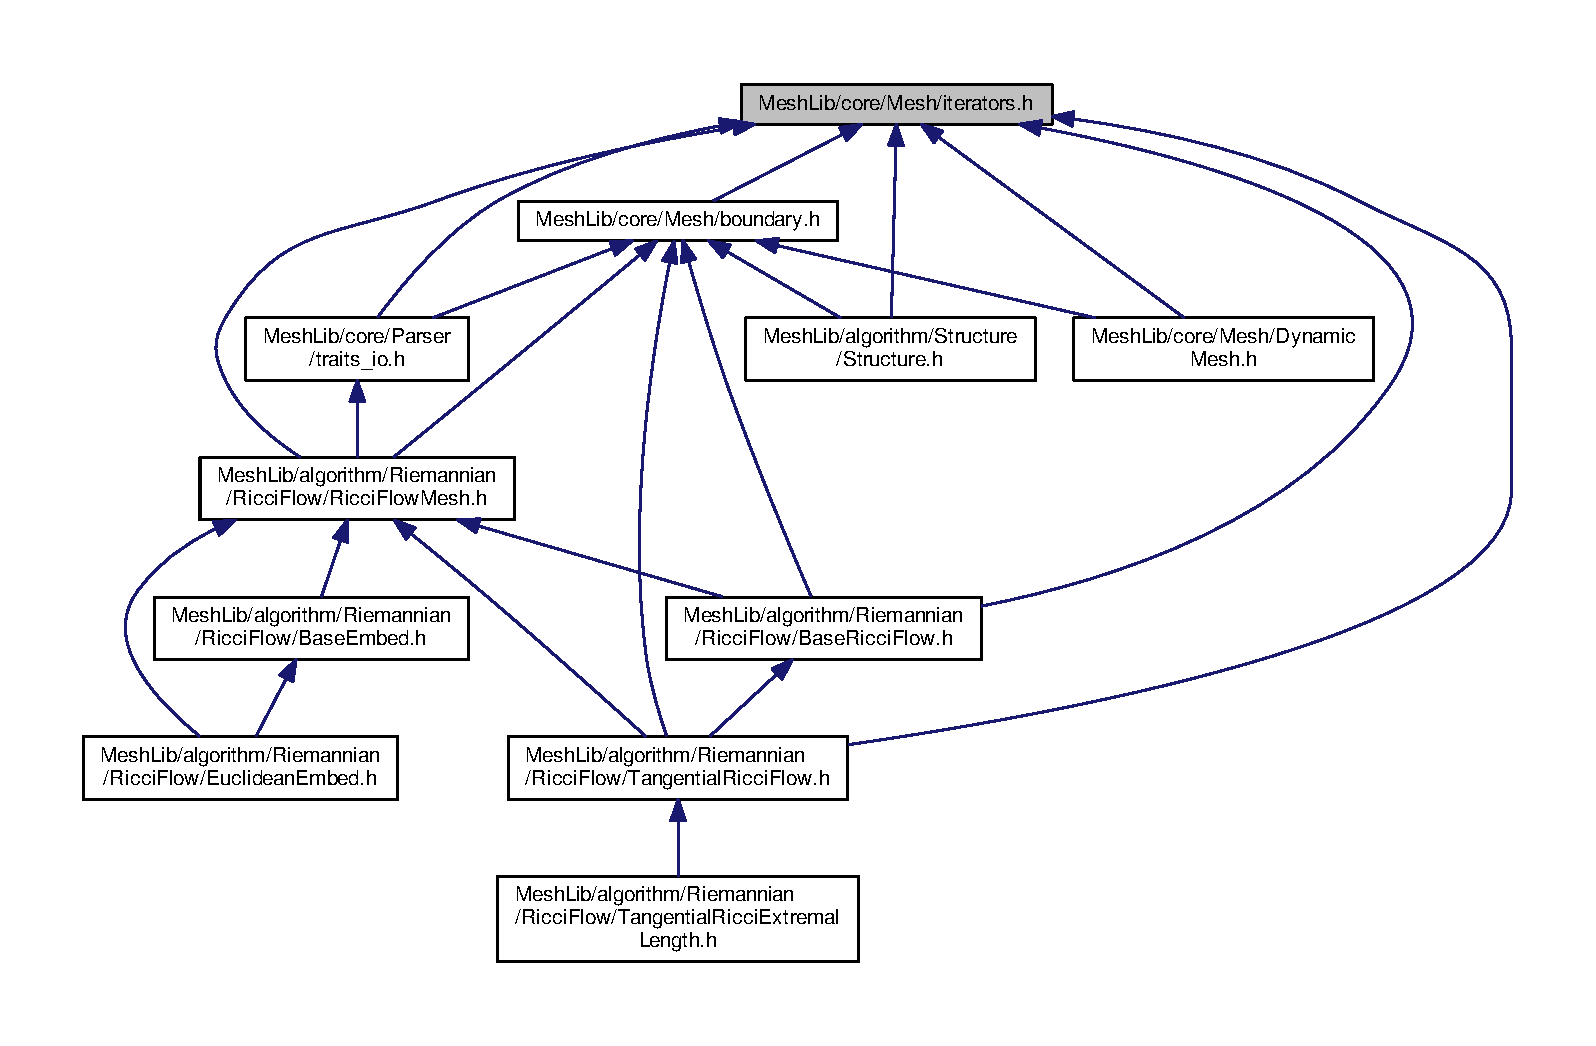
\includegraphics[width=350pt]{iterators_8h__dep__incl}
\end{center}
\end{figure}
\subsection*{Classes}
\begin{DoxyCompactItemize}
\item 
class \hyperlink{class_mesh_lib_1_1_vertex_out_halfedge_iterator}{Mesh\+Lib\+::\+Vertex\+Out\+Halfedge\+Iterator$<$ C\+Vertex, C\+Edge, C\+Face, C\+Half\+Edge $>$}
\begin{DoxyCompactList}\small\item\em \hyperlink{class_mesh_lib_1_1_vertex_out_halfedge_iterator}{Vertex\+Out\+Halfedge\+Iterator}, transverse all the outgoing halfedges of a vertex ccwly. \end{DoxyCompactList}\item 
class \hyperlink{class_mesh_lib_1_1_vertex_in_halfedge_iterator}{Mesh\+Lib\+::\+Vertex\+In\+Halfedge\+Iterator$<$ C\+Vertex, C\+Edge, C\+Face, C\+Half\+Edge $>$}
\begin{DoxyCompactList}\small\item\em \hyperlink{class_mesh_lib_1_1_vertex_in_halfedge_iterator}{Vertex\+In\+Halfedge\+Iterator}, transverse all the incoming halfedges of a vertex ccwly. \end{DoxyCompactList}\item 
class \hyperlink{class_mesh_lib_1_1_vertex_vertex_iterator}{Mesh\+Lib\+::\+Vertex\+Vertex\+Iterator$<$ C\+Vertex, C\+Edge, C\+Face, C\+Half\+Edge $>$}
\begin{DoxyCompactList}\small\item\em \hyperlink{class_mesh_lib_1_1_vertex_vertex_iterator}{Vertex\+Vertex\+Iterator}, transverse all the neighboring vertices of a vertex ccwly. \end{DoxyCompactList}\item 
class \hyperlink{class_mesh_lib_1_1_vertex_edge_iterator}{Mesh\+Lib\+::\+Vertex\+Edge\+Iterator$<$ C\+Vertex, C\+Edge, C\+Face, C\+Half\+Edge $>$}
\begin{DoxyCompactList}\small\item\em \hyperlink{class_mesh_lib_1_1_vertex_edge_iterator}{Vertex\+Edge\+Iterator}, transverse all the neighboring edges of a vertex ccwly. \end{DoxyCompactList}\item 
class \hyperlink{class_mesh_lib_1_1_vertex_face_iterator}{Mesh\+Lib\+::\+Vertex\+Face\+Iterator$<$ C\+Vertex, C\+Edge, C\+Face, C\+Half\+Edge $>$}
\begin{DoxyCompactList}\small\item\em \hyperlink{class_mesh_lib_1_1_vertex_face_iterator}{Vertex\+Face\+Iterator}, transverse all the neighboring faces of a vertex ccwly. \end{DoxyCompactList}\item 
class \hyperlink{class_mesh_lib_1_1_face_halfedge_iterator}{Mesh\+Lib\+::\+Face\+Halfedge\+Iterator$<$ C\+Vertex, C\+Edge, C\+Face, C\+Half\+Edge $>$}
\begin{DoxyCompactList}\small\item\em \hyperlink{class_mesh_lib_1_1_face_halfedge_iterator}{Face\+Halfedge\+Iterator}, transverse all the halfedges of a face C\+C\+Wly. \end{DoxyCompactList}\item 
class \hyperlink{class_mesh_lib_1_1_face_edge_iterator}{Mesh\+Lib\+::\+Face\+Edge\+Iterator$<$ C\+Vertex, C\+Edge, C\+Face, C\+Half\+Edge $>$}
\begin{DoxyCompactList}\small\item\em \hyperlink{class_mesh_lib_1_1_face_edge_iterator}{Face\+Edge\+Iterator}, transverse all the edges of a face C\+C\+Wly. \end{DoxyCompactList}\item 
class \hyperlink{class_mesh_lib_1_1_face_vertex_iterator}{Mesh\+Lib\+::\+Face\+Vertex\+Iterator$<$ C\+Vertex, C\+Edge, C\+Face, C\+Half\+Edge $>$}
\begin{DoxyCompactList}\small\item\em \hyperlink{class_mesh_lib_1_1_face_vertex_iterator}{Face\+Vertex\+Iterator}, transverse all the vertices of a face C\+C\+Wly. \end{DoxyCompactList}\item 
class \hyperlink{class_mesh_lib_1_1_mesh_vertex_iterator}{Mesh\+Lib\+::\+Mesh\+Vertex\+Iterator$<$ C\+Vertex, C\+Edge, C\+Face, C\+Half\+Edge $>$}
\begin{DoxyCompactList}\small\item\em \hyperlink{class_mesh_lib_1_1_mesh_vertex_iterator}{Mesh\+Vertex\+Iterator}, transverse all the vertices in the mesh. \end{DoxyCompactList}\item 
class \hyperlink{class_mesh_lib_1_1_mesh_face_iterator}{Mesh\+Lib\+::\+Mesh\+Face\+Iterator$<$ C\+Vertex, C\+Edge, C\+Face, C\+Half\+Edge $>$}
\begin{DoxyCompactList}\small\item\em \hyperlink{class_mesh_lib_1_1_mesh_face_iterator}{Mesh\+Face\+Iterator}, transverse all the faces in the mesh. \end{DoxyCompactList}\item 
class \hyperlink{class_mesh_lib_1_1_mesh_edge_iterator}{Mesh\+Lib\+::\+Mesh\+Edge\+Iterator$<$ C\+Vertex, C\+Edge, C\+Face, C\+Half\+Edge $>$}
\begin{DoxyCompactList}\small\item\em \hyperlink{class_mesh_lib_1_1_mesh_edge_iterator}{Mesh\+Edge\+Iterator}, transverse all the edges in the mesh. \end{DoxyCompactList}\item 
class \hyperlink{class_mesh_lib_1_1_mesh_half_edge_iterator}{Mesh\+Lib\+::\+Mesh\+Half\+Edge\+Iterator$<$ C\+Vertex, C\+Edge, C\+Face, C\+Half\+Edge $>$}
\begin{DoxyCompactList}\small\item\em \hyperlink{class_mesh_lib_1_1_mesh_half_edge_iterator}{Mesh\+Half\+Edge\+Iterator}, transverse all the halfedges in the mesh. \end{DoxyCompactList}\end{DoxyCompactItemize}
\subsection*{Namespaces}
\begin{DoxyCompactItemize}
\item 
 \hyperlink{namespace_mesh_lib}{Mesh\+Lib}
\end{DoxyCompactItemize}

\hypertarget{_vertex_8h}{}\section{Mesh\+Lib/core/\+Mesh/\+Vertex.h File Reference}
\label{_vertex_8h}\index{Mesh\+Lib/core/\+Mesh/\+Vertex.\+h@{Mesh\+Lib/core/\+Mesh/\+Vertex.\+h}}


Base class of vertex.  


{\ttfamily \#include $<$stdlib.\+h$>$}\\*
{\ttfamily \#include $<$string$>$}\\*
{\ttfamily \#include $<$list$>$}\\*
{\ttfamily \#include \char`\"{}../\+Geometry/\+Point.\+h\char`\"{}}\\*
{\ttfamily \#include \char`\"{}../\+Geometry/\+Point2.\+h\char`\"{}}\\*
{\ttfamily \#include \char`\"{}./\+Half\+Edge.\+h\char`\"{}}\\*
Include dependency graph for Vertex.\+h\+:
\nopagebreak
\begin{figure}[H]
\begin{center}
\leavevmode
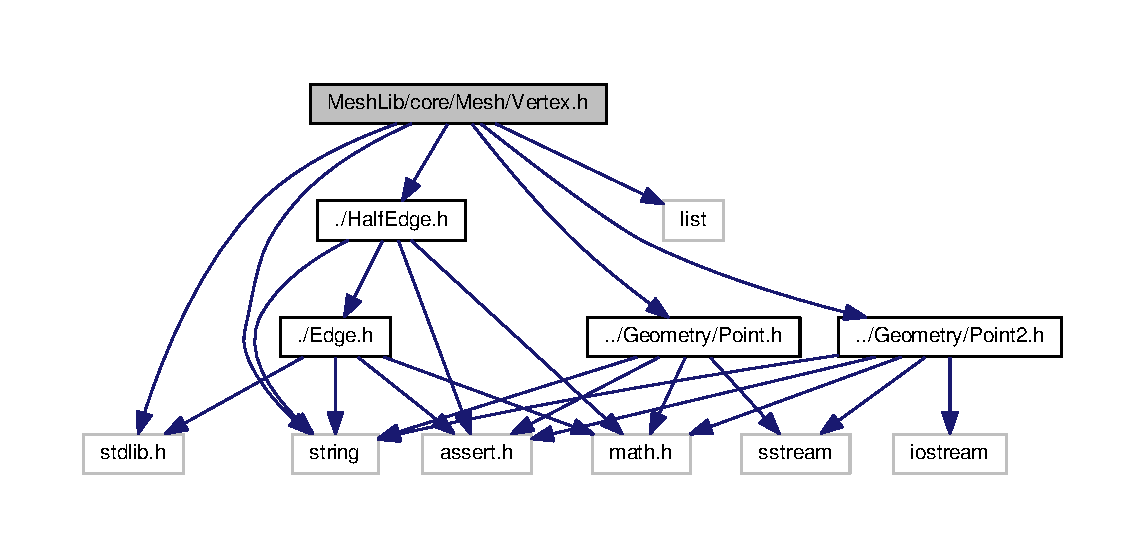
\includegraphics[width=350pt]{_vertex_8h__incl}
\end{center}
\end{figure}
This graph shows which files directly or indirectly include this file\+:
\nopagebreak
\begin{figure}[H]
\begin{center}
\leavevmode
\includegraphics[width=350pt]{_vertex_8h__dep__incl}
\end{center}
\end{figure}
\subsection*{Classes}
\begin{DoxyCompactItemize}
\item 
class \hyperlink{class_mesh_lib_1_1_c_vertex}{Mesh\+Lib\+::\+C\+Vertex}
\begin{DoxyCompactList}\small\item\em \hyperlink{class_mesh_lib_1_1_c_vertex}{C\+Vertex} class, which is the base class of all kinds of vertex classes. \end{DoxyCompactList}\end{DoxyCompactItemize}
\subsection*{Namespaces}
\begin{DoxyCompactItemize}
\item 
 \hyperlink{namespace_mesh_lib}{Mesh\+Lib}
\end{DoxyCompactItemize}


\subsection{Detailed Description}
Base class of vertex. 

\begin{DoxyAuthor}{Author}
David Gu 
\end{DoxyAuthor}
\begin{DoxyDate}{Date}
10/07/2010 
\end{DoxyDate}

\hypertarget{parser_8h}{}\section{Mesh\+Lib/core/\+Parser/parser.h File Reference}
\label{parser_8h}\index{Mesh\+Lib/core/\+Parser/parser.\+h@{Mesh\+Lib/core/\+Parser/parser.\+h}}


Parse the trait strings of vertex, edge, halfedge , face etc.  


{\ttfamily \#include $<$string$>$}\\*
{\ttfamily \#include $<$assert.\+h$>$}\\*
{\ttfamily \#include $<$list$>$}\\*
{\ttfamily \#include $<$sstream$>$}\\*
Include dependency graph for parser.\+h\+:
\nopagebreak
\begin{figure}[H]
\begin{center}
\leavevmode
\includegraphics[width=310pt]{parser_8h__incl}
\end{center}
\end{figure}
This graph shows which files directly or indirectly include this file\+:
\nopagebreak
\begin{figure}[H]
\begin{center}
\leavevmode
\includegraphics[width=350pt]{parser_8h__dep__incl}
\end{center}
\end{figure}
\subsection*{Classes}
\begin{DoxyCompactItemize}
\item 
class \hyperlink{class_mesh_lib_1_1_c_token}{Mesh\+Lib\+::\+C\+Token}
\begin{DoxyCompactList}\small\item\em \hyperlink{class_mesh_lib_1_1_c_token}{C\+Token} class, key=(value), e.\+g. uv=(x y) \end{DoxyCompactList}\item 
class \hyperlink{class_mesh_lib_1_1_c_parser}{Mesh\+Lib\+::\+C\+Parser}
\begin{DoxyCompactList}\small\item\em \hyperlink{class_mesh_lib_1_1_c_parser}{C\+Parser} class. \end{DoxyCompactList}\end{DoxyCompactItemize}
\subsection*{Namespaces}
\begin{DoxyCompactItemize}
\item 
 \hyperlink{namespace_mesh_lib}{Mesh\+Lib}
\end{DoxyCompactItemize}


\subsection{Detailed Description}
Parse the trait strings of vertex, edge, halfedge , face etc. 

\begin{DoxyAuthor}{Author}
David Gu 
\end{DoxyAuthor}
\begin{DoxyDate}{Date}
10/07/2010 
\end{DoxyDate}

\hypertarget{strutil_8h}{}\section{Mesh\+Lib/core/\+Parser/strutil.h File Reference}
\label{strutil_8h}\index{Mesh\+Lib/core/\+Parser/strutil.\+h@{Mesh\+Lib/core/\+Parser/strutil.\+h}}


std\+::string utilities  


{\ttfamily \#include $<$string$>$}\\*
{\ttfamily \#include $<$vector$>$}\\*
{\ttfamily \#include $<$sstream$>$}\\*
{\ttfamily \#include $<$iomanip$>$}\\*
{\ttfamily \#include $<$algorithm$>$}\\*
Include dependency graph for strutil.\+h\+:
\nopagebreak
\begin{figure}[H]
\begin{center}
\leavevmode
\includegraphics[width=350pt]{strutil_8h__incl}
\end{center}
\end{figure}
This graph shows which files directly or indirectly include this file\+:
\nopagebreak
\begin{figure}[H]
\begin{center}
\leavevmode
\includegraphics[width=350pt]{strutil_8h__dep__incl}
\end{center}
\end{figure}
\subsection*{Classes}
\begin{DoxyCompactItemize}
\item 
class \hyperlink{classstrutil_1_1_tokenizer}{strutil\+::\+Tokenizer}
\begin{DoxyCompactList}\small\item\em String \hyperlink{classstrutil_1_1_tokenizer}{Tokenizer}. \end{DoxyCompactList}\end{DoxyCompactItemize}
\subsection*{Namespaces}
\begin{DoxyCompactItemize}
\item 
 \hyperlink{namespacestrutil}{strutil}
\end{DoxyCompactItemize}
\subsection*{Functions}
\begin{DoxyCompactItemize}
\item 
std\+::string \hyperlink{namespacestrutil_ab231c71e590e3a864bcc33b9533a3282}{strutil\+::trim\+Left} (const std\+::string \&str)
\item 
std\+::string \hyperlink{namespacestrutil_af7e41abccf3798fcfc8146dacd6a0e6e}{strutil\+::trim\+Right} (const std\+::string \&str)
\item 
std\+::string \hyperlink{namespacestrutil_ae97dd8d01282a53dff197b2640aaf6a2}{strutil\+::trim} (const std\+::string \&str)
\item 
std\+::string \hyperlink{namespacestrutil_a30dcaa35899109b36dede8d7b65bacb4}{strutil\+::trim} (const std\+::string \&str, const std\+::string \&delimitor)
\item 
std\+::string \hyperlink{namespacestrutil_a33217c775cf7388f4c4e1af1e1fb45a8}{strutil\+::to\+Lower} (const std\+::string \&str)
\item 
std\+::string \hyperlink{namespacestrutil_aa77b45238488b49ad55d2b73294c88ae}{strutil\+::to\+Upper} (const std\+::string \&str)
\item 
bool \hyperlink{namespacestrutil_a5526a6beb76b21d3961809b8ff9d629d}{strutil\+::starts\+With} (const std\+::string \&str, const std\+::string \&substr)
\item 
bool \hyperlink{namespacestrutil_af34e7273311c772c2c0d7b804aa5fb49}{strutil\+::ends\+With} (const std\+::string \&str, const std\+::string \&substr)
\item 
bool \hyperlink{namespacestrutil_a4038560d84d6462679bcd4aaf7499d0e}{strutil\+::equals\+Ignore\+Case} (const std\+::string \&str1, const std\+::string \&str2)
\item 
std\+::string \hyperlink{namespacestrutil_a60b48671666d33f31761ca4fc121c1c4}{strutil\+::to\+String} (const bool \&value)
\item 
{\footnotesize template$<$bool $>$ }\\bool \hyperlink{namespacestrutil_a0776455dafd1a05a3dafc302001d8520}{strutil\+::parse\+String} (const std\+::string \&str)
\item 
{\footnotesize template$<$class T $>$ }\\T \hyperlink{namespacestrutil_ad4e6e4f5f146b8e4c08638557a3d0c3f}{strutil\+::parse\+String} (const std\+::string \&str)
\item 
{\footnotesize template$<$class T $>$ }\\T \hyperlink{namespacestrutil_a28042779b9abcbc8d7b34885b03182d4}{strutil\+::parse\+Hex\+String} (const std\+::string \&str)
\item 
{\footnotesize template$<$class T $>$ }\\std\+::string \hyperlink{namespacestrutil_aea824deca39d542003d5a6b81323f421}{strutil\+::to\+String} (const T \&value)
\item 
{\footnotesize template$<$class T $>$ }\\std\+::string \hyperlink{namespacestrutil_afb6f8558583be9e708aea845d79b4f0e}{strutil\+::to\+Hex\+String} (const T \&value, int width)
\item 
std\+::vector$<$ std\+::string $>$ \hyperlink{namespacestrutil_aa1f64676ef9cc60bfdc94d7ddb86fa5b}{strutil\+::split} (const std\+::string \&str, const std\+::string \&delimiters)
\end{DoxyCompactItemize}


\subsection{Detailed Description}
std\+::string utilities 

\begin{DoxyDate}{Date}
Documented on 10/08/2010 
\end{DoxyDate}

\hypertarget{traits__io_8h}{}\section{Mesh\+Lib/core/\+Parser/traits\+\_\+io.h File Reference}
\label{traits__io_8h}\index{Mesh\+Lib/core/\+Parser/traits\+\_\+io.\+h@{Mesh\+Lib/core/\+Parser/traits\+\_\+io.\+h}}
{\ttfamily \#include $<$map$>$}\\*
{\ttfamily \#include $<$vector$>$}\\*
{\ttfamily \#include $<$complex$>$}\\*
{\ttfamily \#include \char`\"{}../\+Mesh/\+Base\+Mesh.\+h\char`\"{}}\\*
{\ttfamily \#include \char`\"{}../\+Mesh/\+Vertex.\+h\char`\"{}}\\*
{\ttfamily \#include \char`\"{}../\+Mesh/\+Half\+Edge.\+h\char`\"{}}\\*
{\ttfamily \#include \char`\"{}../\+Mesh/\+Edge.\+h\char`\"{}}\\*
{\ttfamily \#include \char`\"{}../\+Mesh/\+Face.\+h\char`\"{}}\\*
{\ttfamily \#include \char`\"{}../\+Mesh/iterators.\+h\char`\"{}}\\*
{\ttfamily \#include \char`\"{}../\+Mesh/boundary.\+h\char`\"{}}\\*
{\ttfamily \#include \char`\"{}./parser.\+h\char`\"{}}\\*
Include dependency graph for traits\+\_\+io.\+h\+:
\nopagebreak
\begin{figure}[H]
\begin{center}
\leavevmode
\includegraphics[width=350pt]{traits__io_8h__incl}
\end{center}
\end{figure}
This graph shows which files directly or indirectly include this file\+:
\nopagebreak
\begin{figure}[H]
\begin{center}
\leavevmode
\includegraphics[width=350pt]{traits__io_8h__dep__incl}
\end{center}
\end{figure}
\subsection*{Namespaces}
\begin{DoxyCompactItemize}
\item 
 \hyperlink{namespace_mesh_lib}{Mesh\+Lib}
\end{DoxyCompactItemize}
\subsection*{Macros}
\begin{DoxyCompactItemize}
\item 
\#define \hyperlink{traits__io_8h_a183c1181dfc37522d163b26bb9402d5d}{V\+E\+R\+T\+E\+X\+\_\+\+R\+GB}~(0x01$<$$<$0)
\item 
\#define \hyperlink{traits__io_8h_ae6080b7459488c1d92b431844323a73b}{V\+E\+R\+T\+E\+X\+\_\+\+UV}~(0x01$<$$<$1)
\item 
\#define \hyperlink{traits__io_8h_adc16f7bc772323ad6b78b831d9e699e9}{V\+E\+R\+T\+E\+X\+\_\+Z}~(0x01$<$$<$2)
\item 
\#define \hyperlink{traits__io_8h_a208e4a865187e8b203b17047065a88c6}{V\+E\+R\+T\+E\+X\+\_\+\+MU}~(0x01$<$$<$3)
\item 
\#define \hyperlink{traits__io_8h_a033cb228ec9541d36a1e74c758225823}{V\+E\+R\+T\+E\+X\+\_\+\+F\+A\+T\+H\+ER}~(0x01$<$$<$4)
\item 
\#define \hyperlink{traits__io_8h_a6ce9e03f5697d5379eea1229ba4a1829}{V\+E\+R\+T\+E\+X\+\_\+\+L\+A\+M\+B\+DA}~(0x01$<$$<$5)
\item 
\#define \hyperlink{traits__io_8h_a5c3a6d59814fce60cac28e5528d2e42a}{V\+E\+R\+T\+E\+X\+\_\+\+N\+O\+R\+M\+AL}~(0x01$<$$<$6)
\item 
\#define \hyperlink{traits__io_8h_a11ed1c0b992e3ed0f708f32733c8b12d}{V\+E\+R\+T\+E\+X\+\_\+U}~(0x01$<$$<$7)
\item 
\#define \hyperlink{traits__io_8h_a362ba25ae42976c0e70ae98a503a12a0}{E\+D\+G\+E\+\_\+\+L\+E\+N\+G\+TH}~(0x01$<$$<$8)
\item 
\#define \hyperlink{traits__io_8h_a3f9edd4dedb7e62a37854d748d9bfb7d}{E\+D\+G\+E\+\_\+\+S\+H\+A\+RP}~(0x01$<$$<$9)
\item 
\#define \hyperlink{traits__io_8h_a9deff46e2667040f0106a1c62e86c616}{E\+D\+G\+E\+\_\+\+DU}~(0x01$<$$<$10)
\item 
\#define \hyperlink{traits__io_8h_a7b145590a6b5cf95dbbbedf0125d6f16}{E\+D\+G\+E\+\_\+\+D\+UV}~(0x01$<$$<$11)
\item 
\#define \hyperlink{traits__io_8h_a38afbd932de159e051d935a8da3eb9b0}{F\+A\+C\+E\+\_\+\+R\+GB}~(0x01$<$$<$16)
\item 
\#define \hyperlink{traits__io_8h_a32d747cbfb5a604d57728c53110e64cc}{F\+A\+C\+E\+\_\+\+N\+O\+R\+M\+AL}~(0x01$<$$<$17)
\end{DoxyCompactItemize}
\subsection*{Functions}
\begin{DoxyCompactItemize}
\item 
{\footnotesize template$<$typename M , typename V , typename E , typename F , typename H $>$ }\\void \hyperlink{namespace_mesh_lib_a92dbd8987379bb2330d0e1dd88541cef}{Mesh\+Lib\+::\+\_\+write\+\_\+vertex\+\_\+uv} (M $\ast$p\+Mesh)
\item 
{\footnotesize template$<$typename M , typename V , typename E , typename F , typename H $>$ }\\void \hyperlink{namespace_mesh_lib_a56e0c746d2f0831f190276f351973eed}{Mesh\+Lib\+::\+\_\+read\+\_\+vertex\+\_\+uv} (M $\ast$p\+Mesh)
\item 
{\footnotesize template$<$typename M , typename V , typename E , typename F , typename H $>$ }\\void \hyperlink{namespace_mesh_lib_a4f1406eba0ac53ede756bca8efacd788}{Mesh\+Lib\+::\+\_\+read\+\_\+vertex\+\_\+z} (M $\ast$p\+Mesh)
\item 
{\footnotesize template$<$typename M , typename V , typename E , typename F , typename H $>$ }\\void \hyperlink{namespace_mesh_lib_a92f633b4ea7e30c040b81dc8895f71e7}{Mesh\+Lib\+::\+\_\+read\+\_\+vertex\+\_\+father} (M $\ast$p\+Mesh)
\item 
{\footnotesize template$<$typename M , typename V , typename E , typename F , typename H $>$ }\\void \hyperlink{namespace_mesh_lib_a7ed997bd5b6fa91b0c9de6129f8b3f5e}{Mesh\+Lib\+::\+\_\+read\+\_\+vertex\+\_\+mu} (M $\ast$p\+Mesh)
\item 
{\footnotesize template$<$typename M , typename V , typename E , typename F , typename H $>$ }\\void \hyperlink{namespace_mesh_lib_a9b33c0e7e2116a58961c6d004cf6799d}{Mesh\+Lib\+::\+\_\+read\+\_\+vertex\+\_\+normal} (M $\ast$p\+Mesh)
\item 
{\footnotesize template$<$typename M , typename V , typename E , typename F , typename H $>$ }\\void \hyperlink{namespace_mesh_lib_aac275eedfecdadd5de1801c33904274f}{Mesh\+Lib\+::\+\_\+read\+\_\+vertex\+\_\+rgb} (M $\ast$p\+Mesh)
\item 
{\footnotesize template$<$typename M , typename V , typename E , typename F , typename H $>$ }\\void \hyperlink{namespace_mesh_lib_a7ce9ef901694368ab52b10d899d4f0a2}{Mesh\+Lib\+::\+\_\+read\+\_\+edge\+\_\+length} (M $\ast$p\+Mesh)
\item 
{\footnotesize template$<$typename M , typename V , typename E , typename F , typename H $>$ }\\void \hyperlink{namespace_mesh_lib_aaf7a33dcbd7f629d69de2d7afb5fcf26}{Mesh\+Lib\+::\+\_\+read\+\_\+edge\+\_\+sharp} (M $\ast$p\+Mesh)
\item 
{\footnotesize template$<$typename M , typename V , typename E , typename F , typename H $>$ }\\void \hyperlink{namespace_mesh_lib_a06158718dbbcbd1ee2b29abe2e606d9c}{Mesh\+Lib\+::\+\_\+write\+\_\+vertex\+\_\+z} (M $\ast$p\+Mesh)
\item 
{\footnotesize template$<$typename M , typename V , typename E , typename F , typename H $>$ }\\void \hyperlink{namespace_mesh_lib_a4bfb121963ba879caaa7c306f33b193f}{Mesh\+Lib\+::\+\_\+write\+\_\+vertex\+\_\+mu} (M $\ast$p\+Mesh)
\item 
{\footnotesize template$<$typename M , typename V , typename E , typename F , typename H $>$ }\\void \hyperlink{namespace_mesh_lib_ae6730ffd9542087c760392db42735aec}{Mesh\+Lib\+::\+\_\+write\+\_\+vertex\+\_\+u} (M $\ast$p\+Mesh)
\item 
{\footnotesize template$<$typename M , typename V , typename E , typename F , typename H $>$ }\\void \hyperlink{namespace_mesh_lib_a2a9154a87dcd05710107028de17b77fd}{Mesh\+Lib\+::\+\_\+write\+\_\+vertex\+\_\+rgb} (M $\ast$p\+Mesh)
\item 
{\footnotesize template$<$typename M , typename V , typename E , typename F , typename H $>$ }\\void \hyperlink{namespace_mesh_lib_aa18d5be66ec31c430180096e99b2c04c}{Mesh\+Lib\+::\+\_\+write\+\_\+edge\+\_\+sharp} (M $\ast$p\+Mesh)
\item 
{\footnotesize template$<$typename M , typename V , typename E , typename F , typename H $>$ }\\void \hyperlink{namespace_mesh_lib_a0420a9c8c7e4fa00c4e43824dcb9a666}{Mesh\+Lib\+::\+\_\+write\+\_\+edge\+\_\+du} (M $\ast$p\+Mesh)
\item 
{\footnotesize template$<$typename M , typename V , typename E , typename F , typename H $>$ }\\void \hyperlink{namespace_mesh_lib_a1ca033523a32826241d6aa0c028d6f3a}{Mesh\+Lib\+::\+\_\+input\+\_\+traits} (M $\ast$p\+Mesh)
\item 
{\footnotesize template$<$typename M , typename V , typename E , typename F , typename H $>$ }\\void \hyperlink{namespace_mesh_lib_a9a2cf62d8e8109d49ebdb83497cf6f91}{Mesh\+Lib\+::\+\_\+output\+\_\+traits} (M $\ast$p\+Mesh)
\end{DoxyCompactItemize}


\subsection{Macro Definition Documentation}
\index{traits\+\_\+io.\+h@{traits\+\_\+io.\+h}!E\+D\+G\+E\+\_\+\+DU@{E\+D\+G\+E\+\_\+\+DU}}
\index{E\+D\+G\+E\+\_\+\+DU@{E\+D\+G\+E\+\_\+\+DU}!traits\+\_\+io.\+h@{traits\+\_\+io.\+h}}
\subsubsection[{\texorpdfstring{E\+D\+G\+E\+\_\+\+DU}{EDGE_DU}}]{\setlength{\rightskip}{0pt plus 5cm}\#define E\+D\+G\+E\+\_\+\+DU~(0x01$<$$<$10)}\hypertarget{traits__io_8h_a9deff46e2667040f0106a1c62e86c616}{}\label{traits__io_8h_a9deff46e2667040f0106a1c62e86c616}


Definition at line 34 of file traits\+\_\+io.\+h.

\index{traits\+\_\+io.\+h@{traits\+\_\+io.\+h}!E\+D\+G\+E\+\_\+\+D\+UV@{E\+D\+G\+E\+\_\+\+D\+UV}}
\index{E\+D\+G\+E\+\_\+\+D\+UV@{E\+D\+G\+E\+\_\+\+D\+UV}!traits\+\_\+io.\+h@{traits\+\_\+io.\+h}}
\subsubsection[{\texorpdfstring{E\+D\+G\+E\+\_\+\+D\+UV}{EDGE_DUV}}]{\setlength{\rightskip}{0pt plus 5cm}\#define E\+D\+G\+E\+\_\+\+D\+UV~(0x01$<$$<$11)}\hypertarget{traits__io_8h_a7b145590a6b5cf95dbbbedf0125d6f16}{}\label{traits__io_8h_a7b145590a6b5cf95dbbbedf0125d6f16}


Definition at line 35 of file traits\+\_\+io.\+h.

\index{traits\+\_\+io.\+h@{traits\+\_\+io.\+h}!E\+D\+G\+E\+\_\+\+L\+E\+N\+G\+TH@{E\+D\+G\+E\+\_\+\+L\+E\+N\+G\+TH}}
\index{E\+D\+G\+E\+\_\+\+L\+E\+N\+G\+TH@{E\+D\+G\+E\+\_\+\+L\+E\+N\+G\+TH}!traits\+\_\+io.\+h@{traits\+\_\+io.\+h}}
\subsubsection[{\texorpdfstring{E\+D\+G\+E\+\_\+\+L\+E\+N\+G\+TH}{EDGE_LENGTH}}]{\setlength{\rightskip}{0pt plus 5cm}\#define E\+D\+G\+E\+\_\+\+L\+E\+N\+G\+TH~(0x01$<$$<$8)}\hypertarget{traits__io_8h_a362ba25ae42976c0e70ae98a503a12a0}{}\label{traits__io_8h_a362ba25ae42976c0e70ae98a503a12a0}


Definition at line 32 of file traits\+\_\+io.\+h.

\index{traits\+\_\+io.\+h@{traits\+\_\+io.\+h}!E\+D\+G\+E\+\_\+\+S\+H\+A\+RP@{E\+D\+G\+E\+\_\+\+S\+H\+A\+RP}}
\index{E\+D\+G\+E\+\_\+\+S\+H\+A\+RP@{E\+D\+G\+E\+\_\+\+S\+H\+A\+RP}!traits\+\_\+io.\+h@{traits\+\_\+io.\+h}}
\subsubsection[{\texorpdfstring{E\+D\+G\+E\+\_\+\+S\+H\+A\+RP}{EDGE_SHARP}}]{\setlength{\rightskip}{0pt plus 5cm}\#define E\+D\+G\+E\+\_\+\+S\+H\+A\+RP~(0x01$<$$<$9)}\hypertarget{traits__io_8h_a3f9edd4dedb7e62a37854d748d9bfb7d}{}\label{traits__io_8h_a3f9edd4dedb7e62a37854d748d9bfb7d}


Definition at line 33 of file traits\+\_\+io.\+h.

\index{traits\+\_\+io.\+h@{traits\+\_\+io.\+h}!F\+A\+C\+E\+\_\+\+N\+O\+R\+M\+AL@{F\+A\+C\+E\+\_\+\+N\+O\+R\+M\+AL}}
\index{F\+A\+C\+E\+\_\+\+N\+O\+R\+M\+AL@{F\+A\+C\+E\+\_\+\+N\+O\+R\+M\+AL}!traits\+\_\+io.\+h@{traits\+\_\+io.\+h}}
\subsubsection[{\texorpdfstring{F\+A\+C\+E\+\_\+\+N\+O\+R\+M\+AL}{FACE_NORMAL}}]{\setlength{\rightskip}{0pt plus 5cm}\#define F\+A\+C\+E\+\_\+\+N\+O\+R\+M\+AL~(0x01$<$$<$17)}\hypertarget{traits__io_8h_a32d747cbfb5a604d57728c53110e64cc}{}\label{traits__io_8h_a32d747cbfb5a604d57728c53110e64cc}


Definition at line 38 of file traits\+\_\+io.\+h.

\index{traits\+\_\+io.\+h@{traits\+\_\+io.\+h}!F\+A\+C\+E\+\_\+\+R\+GB@{F\+A\+C\+E\+\_\+\+R\+GB}}
\index{F\+A\+C\+E\+\_\+\+R\+GB@{F\+A\+C\+E\+\_\+\+R\+GB}!traits\+\_\+io.\+h@{traits\+\_\+io.\+h}}
\subsubsection[{\texorpdfstring{F\+A\+C\+E\+\_\+\+R\+GB}{FACE_RGB}}]{\setlength{\rightskip}{0pt plus 5cm}\#define F\+A\+C\+E\+\_\+\+R\+GB~(0x01$<$$<$16)}\hypertarget{traits__io_8h_a38afbd932de159e051d935a8da3eb9b0}{}\label{traits__io_8h_a38afbd932de159e051d935a8da3eb9b0}


Definition at line 37 of file traits\+\_\+io.\+h.

\index{traits\+\_\+io.\+h@{traits\+\_\+io.\+h}!V\+E\+R\+T\+E\+X\+\_\+\+F\+A\+T\+H\+ER@{V\+E\+R\+T\+E\+X\+\_\+\+F\+A\+T\+H\+ER}}
\index{V\+E\+R\+T\+E\+X\+\_\+\+F\+A\+T\+H\+ER@{V\+E\+R\+T\+E\+X\+\_\+\+F\+A\+T\+H\+ER}!traits\+\_\+io.\+h@{traits\+\_\+io.\+h}}
\subsubsection[{\texorpdfstring{V\+E\+R\+T\+E\+X\+\_\+\+F\+A\+T\+H\+ER}{VERTEX_FATHER}}]{\setlength{\rightskip}{0pt plus 5cm}\#define V\+E\+R\+T\+E\+X\+\_\+\+F\+A\+T\+H\+ER~(0x01$<$$<$4)}\hypertarget{traits__io_8h_a033cb228ec9541d36a1e74c758225823}{}\label{traits__io_8h_a033cb228ec9541d36a1e74c758225823}


Definition at line 28 of file traits\+\_\+io.\+h.

\index{traits\+\_\+io.\+h@{traits\+\_\+io.\+h}!V\+E\+R\+T\+E\+X\+\_\+\+L\+A\+M\+B\+DA@{V\+E\+R\+T\+E\+X\+\_\+\+L\+A\+M\+B\+DA}}
\index{V\+E\+R\+T\+E\+X\+\_\+\+L\+A\+M\+B\+DA@{V\+E\+R\+T\+E\+X\+\_\+\+L\+A\+M\+B\+DA}!traits\+\_\+io.\+h@{traits\+\_\+io.\+h}}
\subsubsection[{\texorpdfstring{V\+E\+R\+T\+E\+X\+\_\+\+L\+A\+M\+B\+DA}{VERTEX_LAMBDA}}]{\setlength{\rightskip}{0pt plus 5cm}\#define V\+E\+R\+T\+E\+X\+\_\+\+L\+A\+M\+B\+DA~(0x01$<$$<$5)}\hypertarget{traits__io_8h_a6ce9e03f5697d5379eea1229ba4a1829}{}\label{traits__io_8h_a6ce9e03f5697d5379eea1229ba4a1829}


Definition at line 29 of file traits\+\_\+io.\+h.

\index{traits\+\_\+io.\+h@{traits\+\_\+io.\+h}!V\+E\+R\+T\+E\+X\+\_\+\+MU@{V\+E\+R\+T\+E\+X\+\_\+\+MU}}
\index{V\+E\+R\+T\+E\+X\+\_\+\+MU@{V\+E\+R\+T\+E\+X\+\_\+\+MU}!traits\+\_\+io.\+h@{traits\+\_\+io.\+h}}
\subsubsection[{\texorpdfstring{V\+E\+R\+T\+E\+X\+\_\+\+MU}{VERTEX_MU}}]{\setlength{\rightskip}{0pt plus 5cm}\#define V\+E\+R\+T\+E\+X\+\_\+\+MU~(0x01$<$$<$3)}\hypertarget{traits__io_8h_a208e4a865187e8b203b17047065a88c6}{}\label{traits__io_8h_a208e4a865187e8b203b17047065a88c6}


Definition at line 27 of file traits\+\_\+io.\+h.

\index{traits\+\_\+io.\+h@{traits\+\_\+io.\+h}!V\+E\+R\+T\+E\+X\+\_\+\+N\+O\+R\+M\+AL@{V\+E\+R\+T\+E\+X\+\_\+\+N\+O\+R\+M\+AL}}
\index{V\+E\+R\+T\+E\+X\+\_\+\+N\+O\+R\+M\+AL@{V\+E\+R\+T\+E\+X\+\_\+\+N\+O\+R\+M\+AL}!traits\+\_\+io.\+h@{traits\+\_\+io.\+h}}
\subsubsection[{\texorpdfstring{V\+E\+R\+T\+E\+X\+\_\+\+N\+O\+R\+M\+AL}{VERTEX_NORMAL}}]{\setlength{\rightskip}{0pt plus 5cm}\#define V\+E\+R\+T\+E\+X\+\_\+\+N\+O\+R\+M\+AL~(0x01$<$$<$6)}\hypertarget{traits__io_8h_a5c3a6d59814fce60cac28e5528d2e42a}{}\label{traits__io_8h_a5c3a6d59814fce60cac28e5528d2e42a}


Definition at line 30 of file traits\+\_\+io.\+h.

\index{traits\+\_\+io.\+h@{traits\+\_\+io.\+h}!V\+E\+R\+T\+E\+X\+\_\+\+R\+GB@{V\+E\+R\+T\+E\+X\+\_\+\+R\+GB}}
\index{V\+E\+R\+T\+E\+X\+\_\+\+R\+GB@{V\+E\+R\+T\+E\+X\+\_\+\+R\+GB}!traits\+\_\+io.\+h@{traits\+\_\+io.\+h}}
\subsubsection[{\texorpdfstring{V\+E\+R\+T\+E\+X\+\_\+\+R\+GB}{VERTEX_RGB}}]{\setlength{\rightskip}{0pt plus 5cm}\#define V\+E\+R\+T\+E\+X\+\_\+\+R\+GB~(0x01$<$$<$0)}\hypertarget{traits__io_8h_a183c1181dfc37522d163b26bb9402d5d}{}\label{traits__io_8h_a183c1181dfc37522d163b26bb9402d5d}


Definition at line 24 of file traits\+\_\+io.\+h.

\index{traits\+\_\+io.\+h@{traits\+\_\+io.\+h}!V\+E\+R\+T\+E\+X\+\_\+U@{V\+E\+R\+T\+E\+X\+\_\+U}}
\index{V\+E\+R\+T\+E\+X\+\_\+U@{V\+E\+R\+T\+E\+X\+\_\+U}!traits\+\_\+io.\+h@{traits\+\_\+io.\+h}}
\subsubsection[{\texorpdfstring{V\+E\+R\+T\+E\+X\+\_\+U}{VERTEX_U}}]{\setlength{\rightskip}{0pt plus 5cm}\#define V\+E\+R\+T\+E\+X\+\_\+U~(0x01$<$$<$7)}\hypertarget{traits__io_8h_a11ed1c0b992e3ed0f708f32733c8b12d}{}\label{traits__io_8h_a11ed1c0b992e3ed0f708f32733c8b12d}


Definition at line 31 of file traits\+\_\+io.\+h.

\index{traits\+\_\+io.\+h@{traits\+\_\+io.\+h}!V\+E\+R\+T\+E\+X\+\_\+\+UV@{V\+E\+R\+T\+E\+X\+\_\+\+UV}}
\index{V\+E\+R\+T\+E\+X\+\_\+\+UV@{V\+E\+R\+T\+E\+X\+\_\+\+UV}!traits\+\_\+io.\+h@{traits\+\_\+io.\+h}}
\subsubsection[{\texorpdfstring{V\+E\+R\+T\+E\+X\+\_\+\+UV}{VERTEX_UV}}]{\setlength{\rightskip}{0pt plus 5cm}\#define V\+E\+R\+T\+E\+X\+\_\+\+UV~(0x01$<$$<$1)}\hypertarget{traits__io_8h_ae6080b7459488c1d92b431844323a73b}{}\label{traits__io_8h_ae6080b7459488c1d92b431844323a73b}


Definition at line 25 of file traits\+\_\+io.\+h.

\index{traits\+\_\+io.\+h@{traits\+\_\+io.\+h}!V\+E\+R\+T\+E\+X\+\_\+Z@{V\+E\+R\+T\+E\+X\+\_\+Z}}
\index{V\+E\+R\+T\+E\+X\+\_\+Z@{V\+E\+R\+T\+E\+X\+\_\+Z}!traits\+\_\+io.\+h@{traits\+\_\+io.\+h}}
\subsubsection[{\texorpdfstring{V\+E\+R\+T\+E\+X\+\_\+Z}{VERTEX_Z}}]{\setlength{\rightskip}{0pt plus 5cm}\#define V\+E\+R\+T\+E\+X\+\_\+Z~(0x01$<$$<$2)}\hypertarget{traits__io_8h_adc16f7bc772323ad6b78b831d9e699e9}{}\label{traits__io_8h_adc16f7bc772323ad6b78b831d9e699e9}


Definition at line 26 of file traits\+\_\+io.\+h.


%--- End generated contents ---

% Index
\backmatter
\newpage
\phantomsection
\clearemptydoublepage
\addcontentsline{toc}{chapter}{Index}
\printindex

\end{document}
